\documentclass[tocnosub, noragright, centerchapter, mixcasechap, 12pt]{../uiucecethesis09}

\pdfmapline{+dummy-space <dummy-space.pfb}

% Use offcenter for the extra .5 inch on the left side. Needed with fullpage and fancy.
% Use mixcasechap for compatibility with hyperref package, which does NOT like all caps default
% Use edeposit for the adviser/committee on the title page.

\makeatletter

%--------------------------------------
% USEPACKAGE COMMANDS
% GUIDELINES: packages in alphabetical order with a comment providing a high-level description of the package

% needs to be loaded first
\usepackage[hyphens]{url} % hyphenation of URLs

% https://tex.stackexchange.com/questions/66958/how-do-you-suppress-specific-warnings-generated-by-pdflatex
\usepackage{silence}
\WarningFilter[pdftoc]{hyperref}{Token not allowed in a PDF string (Unicode)}
\ActivateWarningFilters[pdftoc]

% normal
\usepackage[resetcount,algochapter]{algorithm2e} % environment for algorithms 
\usepackage{amsmath} % AMS mathematical facilities for LATEX
\usepackage{amssymb} % 
\usepackage{amsfonts} % TEX fonts from the American Mathematical Society
\usepackage[american]{babel} % culturally determined typographical rules
\usepackage{bm} % bold for greek symbols
\usepackage{caption} % makes captions ragged right
\usepackage{subcaption} % support for subcaptions
\usepackage{enumitem} % controls enumerate, itemize and description
\usepackage{graphicx} % another package that works for figures
\usepackage{geometry} % customize page layout
\usepackage{lscape} % modifies the margins and rotates the page locally
\usepackage{mathtools} % mathematical tools to use with amsmath
\usepackage{setspace} % set space between lines
\usepackage[dvipsnames]{xcolor} % defines colors
\usepackage{blindtext} % produces text for testing
\usepackage{import} % establish input relative to a directory
\usepackage{epigraph} % pithy quotations
\usepackage{nicefrac} % typesets fractions 'nicely'
\usepackage{etoolbox} % toolbox of programming facilities
\usepackage{subfiles} % typesetting a multi-file project
\usepackage{xpatch} % for patching biblatex
\usepackage[T1]{fontenc} % change font encoding
\usepackage{lmodern} % use latin modern fonts


\usepackage{chngcntr}
\counterwithout{footnote}{chapter}

\usepackage[normalem]{ulem}

% \usepackage{stringstrings}

%-------------------------------------------------
% from DETC2017-67668 Co-Design Theory Paper
%-------------------------------------------------
\usepackage{ltxcmds}
\usepackage{ifthen}
\usepackage{cancel}
\usepackage{empheq}
\usepackage{fontawesome}
%-------------------------------------------------


%-------------------------------------------------
% from DETC2017-67676 Scaling Paper
%-------------------------------------------------
% \usepackage{nomencl}
%-------------------------------------------------

%-------------------------------------------------
% from MD-16-1635 PM Architectures Paper
%-------------------------------------------------
\usepackage{float}
\restylefloat{table}
\usepackage[export]{adjustbox}
\usepackage{varwidth}
\usepackage{relsize}
\usepackage{tkz-linknodes}
\usepackage{rotating}
\usepackage{tikz} % for drawings
\usetikzlibrary{shapes.geometric, arrows, topaths, shapes,decorations.text, positioning,shadows,trees,shapes.arrows, fadings,arrows.meta,graphs,graphs.standard}
% \usetikzlibrary{external}
\usepackage{blkarray}
%-------------------------------------------------

%-------------------------------------------------
% from PM Enhancements Paper
%-------------------------------------------------
\usepackage{amsthm} % theorem-like structures
% \usepackage[strict]{changepage} % change the page layout in the middle of a document 
\usepackage{epstopdf} % 'include' eps files 
\usepackage{framed} % framed or shaded regions
% \usepackage{lastpage} % reference to the last page
\usepackage{pifont} % Pi fonts (Dingbats, Symbol, etc)
\usepackage{titlesec} % alternative section titles
\usepackage{verbatim} % displays verbatim text 
\usepackage{xstring} % provides macros for manipulating strings 
%-------------------------------------------------

%-------------------------------------------------
% from PM circuits paper
%-------------------------------------------------
\usepackage{multirow}
%-------------------------------------------------

%-------------------------------------------------
% from DT QP paper
%-------------------------------------------------
% \usepackage{tikz} % drawings
\usetikzlibrary{shapes,arrows,positioning,snakes,arrows.meta}
\usetikzlibrary{matrix}
\usetikzlibrary{arrows,shapes,positioning, shapes.symbols}
\usetikzlibrary{calc,decorations.markings, decorations.pathreplacing}
% \usetikzlibrary{external}
% \tikzexternalize[prefix=../_main/tikz/]
\usepackage{matlab-prettifier}
%-------------------------------------------------

%-------------------------------------------------
% tikz_options
% for references

\usepackage{tkz-linknodes}

\usepackage{tikz} % load the package

\usetikzlibrary{shapes.geometric, arrows, topaths, shapes,decorations.text, positioning,shadows,trees,shapes.arrows, fadings,arrows.meta,graphs,graphs.standard}

\usetikzlibrary{external} % drawings
% bibtex_options
% for references

\usepackage[
backend = bibtex, 
bibstyle = ieee, 
citestyle = numeric-comp,
backref = true,
hyperref = true,
maxcitenames = 3,
maxbibnames = 3,
block = none,
]{biblatex} % for references

% other potential options
% bibstyle=ieee-alphabetic, 
% citestyle=alphabetic,

\DefineBibliographyStrings{english}{
  backrefpage  = {see p\adddot},
  backrefpages = {see pp\adddot},
  url = {url},
  phdthesis = {PhD dissertation},
}

% remove period at the end of the citations
\renewcommand*{\finentrypunct}{}

% change font size
\renewcommand*{\bibfont}{\footnotesize}

% customize the doi field
\DeclareFieldFormat{doi}{%
  \printtext{doi}\addcolon\space
    \ifhyperref
      {\href{http://dx.doi.org/#1}{\nolinkurl{#1}}}
      {\nolinkurl{#1}}}

% change isbn field
\DeclareFieldFormat{isbn}{%
	\printtext{isbn}\addcolon\space{#1}}

\xpatchbibdriver{online}
  {\printtext[parens]{\usebibmacro{date}}}
  {\iffieldundef{year}{}{\printtext[parens]{\usebibmacro{date}}}}
  {}{} % references
% Two Column Compatible, Variable Width Algorithm Environments
% Written by Daniel Herber
% Based on modifications to the stack exchange answer at
% http://tex.stackexchange.com/questions/23296/setting-caption-rule-width-in-algorithm2e-algs/39574

% inputs
% 1 : float specifiers (htbp!)
% 2 : algorithm width (length)
% 3 : indent width (length)

% column environment
% \begin{vAlgorithm}[float specifiers]{algorithm width}{indent width}
% \end{vAlgorithm}

% page environment
% \begin{vAlgorithm*}[float specifiers]{algorithm width}{indent width}
% \end{vAlgorithm*}

% required packages
\usepackage{algorithm2e}
\usepackage{etoolbox}
\usepackage{xstring}
\usepackage{calc}
 
% define lengths
\newlength{\xalgowidth}
\newlength{\xalgoremainder}
\newlength{\xindentwidth}

% define vAlgorithm* environment
\newenvironment{vAlgorithm*}[3][]{% before
  \setlength{\xalgowidth}{#2} % set algorithm width from second input
  \setlength{\xindentwidth}{#3} % set indent width from third input
  \setlength{\xalgoremainder}{\textwidth-\xalgowidth} % calculate indent to center the float
  \SetCustomAlgoRuledWidth{\xalgowidth} % set the rule width
  \IncMargin{\xindentwidth}
  \begin{algorithm*}[#1]
}% end before
{% after
  \end{algorithm*} 
  \DecMargin{\xindentwidth}
}% end after

% define vAlgorithm environment
\newenvironment{vAlgorithm}[3][]{% before
  \setlength{\xalgowidth}{#2} % set algorithm width from second input
  \setlength{\xindentwidth}{#3} % set indent width from third input
  \setlength{\xalgoremainder}{\columnwidth-\xalgowidth} % calculate indent to center the float
  \SetCustomAlgoRuledWidth{\xalgowidth} % set the rule width
  \IncMargin{\xindentwidth}
  \begin{algorithm}[#1] % column
}% end before
{% after
  \end{algorithm} % column
  \DecMargin{\xindentwidth}
}% end after

% redefine algorithm commands
\makeatletter
\patchcmd{\@algocf@start}{%
\begin{lrbox}{\algocf@algobox}%
}{%
\rule{0.5\xalgoremainder}{\z@}% indent
\begin{lrbox}{\algocf@algobox}%
\begin{minipage}{\xalgowidth}%
}{}{}
\patchcmd{\@algocf@finish}{%
\end{lrbox}%
}{%
\end{minipage}%
\end{lrbox}%
}{}{}
\makeatother % algorithm environment
% local packages
\usepackage{algorithm2e}
\usepackage{xcolor}

%----------------------------------
% custom style commands
%----------------------------------
% variable style command
\newcommand{\xvar}[1]{\textup{\textsf{#1}}}

% horizontal alignment command
\newcommand{\xvbox}[2]{\makebox[#1][l]{#2}}

%----------------------------------
% set algorithm2e styles
%----------------------------------
% change algorithm font size
\SetAlFnt{\footnotesize}

% change algorithm caption style
\newcommand{\xAlCapSty}[1]{\bfseries#1}
\SetAlCapSty{xAlCapSty}

% comment style (algorithms)
% \newcommand{\xCommentSty}[1]{\scriptsize\ttfamily\textcolor{blue}{#1}}
\definecolor{commentcolor}{RGB}{27, 94, 32}
\newcommand{\xCommentSty}[1]{\scriptsize\ttfamily\textcolor{commentcolor}{#1}}
\SetCommentSty{xCommentSty}

% function style
\newcommand{\xFuncSty}[1]{#1}
% \SetProgSty{textnormal}
% \SetArgSty{textnormal}

% change line number style
% \newcommand\mynlfont[1]{\scriptsize\sffamily{#1}}
\newcommand\mynlfont[1]{\sffamily{#1}}
\SetNlSty{mynlfont}{}{} 

 % add the line numbers
\LinesNumbered

% comments right justified
\SetSideCommentRight

% don't print semicolon
\DontPrintSemicolon

% ruled algorithm
\RestyleAlgo{algoruled} % algorithm style
%-------------------------------------------------

%-----------------------------------------------------
% LATER PACKAGES
% hyperref_options
% 
% needs to be after biblatex package

\usepackage[hidelinks,pdfencoding=auto]{hyperref} 

\hypersetup{
    bookmarks = true,         % show bookmarks bar?
    bookmarksnumbered = true,
    % unicode = false,          % non-Latin characters in Acrobat’s bookmarks
    pdftoolbar = true,        % show Acrobat’s toolbar?
    pdfmenubar = true,        % show Acrobat’s menu?
    pdffitwindow = false,     % window fit to page when opened
    pdfstartview = {FitV},    % fits the width of the page to the window
    pdftitle = {Advances in Combined Architecture, Plant, and Control Design},    % title
    pdfauthor = {Daniel Ronald Herber},     % author
    pdfsubject = {Ph.D. Dissertation},   % subject of the document
    pdfdisplaydoctitle = true,
    pdfkeywords = {}, % list of keywords
    pdfnewwindow = true,      % links in new window
    pdfstartpage = {2}, 
    pdfhighlight = {/I},
}

\hypersetup{colorlinks = true, allcolors = blue}

% https://tex.stackexchange.com/questions/142251/hyperref-token-not-allowed-warning-possible-bug % hyperlinks 

%-------------------------------------------------
% glossaries
%-------------------------------------------------
% https://tex.stackexchange.com/questions/28797/links-to-glossary-items-broken/28800
% \usepackage[automake, acronyms, nogroupskip, indexonlyfirst]{glossaries} % glossaries
% \usepackage[automake, acronyms, nogroupskip]{glossaries} % glossaries

\usepackage[automake, acronyms, nogroupskip, indexonlyfirst]{glossaries-extra} % glossaries

\newglossary{symbol}{sym}{sbl}{List of Symbols}
\newglossary{notation}{not}{ntn}{List of General Notation}
\makeglossaries
\glsenablehyper

\glsaddkey
 {foo}% new key
 {\relax}% default value if "foo" isn't used in \newglossaryentry
 {\glsentryfoo}% analogous to \glsentrytext
 {\Glsentryfoo}% analogous to \Glsentrytext
 {\glsfoo}% analogous to \glstext
 {\Glsfoo}% analogous to \Glstext
 {\GLSfoo}% analogous to \GLStext

\loadglsentries{../gls/notation}
\loadglsentries{../gls/acronyms}
\loadglsentries{../gls/symbols}

\newglossarystyle{glossymbol}{%
    \renewenvironment{theglossary}{% Change the table type --> 3 columns
        \begin{longtable}{r p{4.75in} r}}%
        {\end{longtable}}%
    \renewcommand*{\glossaryheader}{%  Change the table header
        \bfseries Symbol & \bfseries Description & \bfseries Page \\
              \hline
        \endhead}
    \renewcommand*{\glossentry}[2]{%  Change the displayed items
        \glstarget{##1}{\glossentryname{##1}} %
        & \glossentrydesc{##1} 
        & {##2} 
         \tabularnewline
    }
}
\newglossarystyle{glosacronym}{%
    \renewenvironment{theglossary}{% Change the table type --> 3 columns
        \begin{longtable}{r p{3.25in} r}}%
        {\end{longtable}}%
    \renewcommand*{\glossaryheader}{%  Change the table header
        \bfseries Abbreviations & \bfseries Description & \bfseries Page \\
              \hline
        \endhead}
    \renewcommand*{\glossentry}[2]{%  Change the displayed items
        \glstarget{##1}{\glossentryname{##1}} %
        & \glossentrydesc{##1} 
        & {##2} 
         \tabularnewline
    }
}
\newglossarystyle{glosnotation}{%
    \renewenvironment{theglossary}{% Change the table type --> 3 columns
        \begin{longtable}{r p{2.75in} r}}%
        {\end{longtable}}%
    \renewcommand*{\glossaryheader}{%  Change the table header
        \bfseries Notation & \bfseries Description & \bfseries Page \\
              \hline
        \endhead}
    \renewcommand*{\glossentry}[2]{%  Change the displayed items
        \glstarget{##1}{\glossentryname{##1}} %
        & \glossentrydesc{##1} 
        & {##2} 
         \tabularnewline
    }
}

% \usepackage{showframe} % show page frames
% \usepackage{lineno} % include line numbers 
%--------------------------------------
% CUSTOM COMMANDS

% thesis document
\newcommand{\mychapter}[1]{\chapter{#1}}
\newcommand{\mychapterfoot}[1]{\chapter[#1]{#1\texorpdfstring{\footnotemark{}}{}}}

% font styles
\newcommand{\xcolor}[1]{\textsl{\textsf{#1}}} % colored graph labels
% \newcommand{\xvar}[1]{\textup{\textsf{#1}}} % code variables in AlgorithmStyle
\newcommand{\xprog}[1]{\textsc{#1}} % programs

% editing
\newcommand{\xrev}[1]{\textcolor{red}{#1}} % revision
\newcommand{\xneed}[1]{\textcolor{red}{\textbf{#1}}} % need to address

% colors
\definecolor{light-gray}{gray}{0.8}
\definecolor{uiuc-orange-1}{HTML}{FA6300}
\definecolor{uiuc-orange-2}{HTML}{E14A00}

% epigraph
\renewcommand{\epigraphflush}{flushleft}
\renewcommand{\sourceflush}{flushleft}
\setlength{\epigraphwidth}{0.8\textwidth}

% change equation spacing
\expandafter\def\expandafter\normalsize\expandafter{%
    \normalsize
    \setlength\abovedisplayskip{8pt}
    \setlength\belowdisplayskip{8pt}
    \setlength\abovedisplayshortskip{8pt}
    \setlength\belowdisplayshortskip{8pt}
}

\newcommand{\cfbox}[2]{%
#2
%    \colorlet{currentcolor}{.}%
%    {\color{#1}%
%    \fbox{\color{currentcolor}#2}}%
}

% spacing

% indexing (algorithms)
\newcommand{\myind}[1]{$\langle${#1}$\rangle$}


\newcommand{\bL}{\bm{L}}
\newcommand{\bl}{\bm{l}}
\newcommand{\bM}{\bm{M}}
\newcommand{\bmm}{\bm{m}}

\newcommand{\breakline}{\vspace{-1ex}\begin{center}\noindent\rule{0.6\columnwidth}{0.4pt}\end{center}}

%-------------------------------------------------
% from DETC2017-67668 Co-Design Theory Paper
%-------------------------------------------------
\definecolor{light-gray}{gray}{0.4}
\definecolor{box-gray}{gray}{1}
\newcommand{\bxi}{\bm{\xi}}
\newcommand{\bxp}{\bm{x}_p}
\newcommand{\bxc}{\bm{x}_c}
\newcommand{\bu}{\bm{u}}
\newcommand{\bp}{\bm{p}}
\newcommand{\bfd}{\bm{f}}
\newcommand{\bzero}{\bm{0}}
\newcommand{\blambda}{\bm{\lambda}}
\newcommand{\bmu}{\bm{\mu}}
\newcommand{\bnu}{\bm{\nu}}
\newcommand{\lagrange}{\mathcal{L}}
\newcommand{\mayer}{\mathcal{M}}
\newcommand{\eqtextcolor}[1]{\text{\textcolor{black!30}{#1}}}
\newcommand{\pd}[2]{\frac{\partial #1}{\partial #2}}
\newcommand{\der}[2]{\frac{d #1}{d #2}}
%-------------------------------------------------

%-------------------------------------------------
% from DETC2017-67676 Scaling Paper
%-------------------------------------------------
\newcommand{\mybar}[1]{\bar{#1}}
%-------------------------------------------------

%-------------------------------------------------
% from MD-16-1635 PM Architectures Paper
%-------------------------------------------------
% \newcommand{\mypm}{\textit{PM}}
\newcommand{\mypm}{PM}
\newtheorem{definition}{Definition}
% \definecolor{light-gray}{gray}{0.8}
% \newcommand{\xcolor}[1]{\text{\textsl{\textsf{#1}}}}
\newcommand\scalemath[2]{\scalebox{#1}{\mbox{\ensuremath{\displaystyle #2}}}}   
\newcommand*\circled[1]{\tikz[baseline=(char.base)]{
            \node[shape=circle,draw,inner sep=1pt] (char) {\small #1};}}
\newcommand\hlight[2]{\tikz[overlay, remember picture,baseline=-\the\dimexpr\fontdimen22\textfont2\relax]\node[rectangle,fill=black!#2,rounded corners,fill opacity = 0.8,thick,text opacity =1] {$#1$};} 
\newcommand{\tikzmark}[2]{
    \tikz[overlay,remember picture,baseline] 
    \node[anchor=base] (#1) {$#2$};
}
%-------------------------------------------------

%-------------------------------------------------
% from DT QP paper
%-------------------------------------------------
\newcommand{\qp}{QP}
\newcommand{\lqdo}{LQDO}
\newcommand{\dt}{DT}
\newcommand{\apgp}{APGP}
\newcommand*{\tran}{^{\mkern-1.5mu\mathsf{T}}}
\newcommand{\overbar}[1]{\mkern 1.5mu\overline{\mkern-1.5mu#1\mkern-1.5mu}\mkern 1.5mu}
\newcommand{\myoverbar}[1]{\mkern 1.5mu\overline{\mkern-1.5mu#1\mkern-1.5mu}\mkern 1.5mu} %  alternative to \bar{} command
\newcommand{\myunderbar}[1]{\mkern 1.5mu\underline{\mkern-1.5mu#1\mkern-1.5mu}\mkern 1.5mu} %  alternative to \bar{} command
\newenvironment{lbmatrix}[1]
  {\left[\array{@{}*{#1}{c}@{}}}
  {\endarray\right]}

\newcommand{\xind}[1]{\langle{#1}\rangle}
\newcommand{\mysparsesymbol}{\textcolor{black!20}{$\bullet$}}
\newcommand{\mytemp}{\textcolor{black}{$\bullet$}}
\newcommand{\mysparseboxcolor}{black!20}
\def\Vhrulefill{\leavevmode\leaders\hrule height 0.7ex depth \dimexpr0.4pt-0.7ex\hfill\kern0pt}

%-------------------------------------------------

% --- mathtools ---------------------------------
\DeclarePairedDelimiter\abs{\lvert}{\rvert} % absolute value delimiter
\DeclarePairedDelimiter\norm{\lVert}{\rVert} % norm delimiter 

% captions
\captionsetup{labelfont=bf, justification=raggedright}

\setcounter{secnumdepth}{3} % include subsubsection in numbering

\usepackage[titles]{tocloft}
\renewcommand{\contentsname}{Table of contents}
\renewcommand{\cftchapfont}{\normalfont\bfseries}% titles in bold
\renewcommand{\cftchappagefont}{\normalfont\bfseries}% page numbers in bold
\renewcommand{\cftdotsep}{1}
\renewcommand{\cftchapleader}{\cftdotfill{\cftsecdotsep}}% dot leaders in bold
\setcounter{tocdepth}{1}

% \titleformat{\chapter}[display]
%         {\normalfont}{\chaptertitlename\ \thechapter}{0pt}{\normalfont}

% for allison
\definecolor{jta}{RGB}{183, 28, 28}
% \newcommand{\JTA}[1]{\textcolor{jta}{$\prescript{\text{(JTA)}}{}{}$}\textcolor{jta}{#1}}
% \definecolor{linkcolor}{RGB}{40, 53, 147}
% \definecolor{linkcolor}{RGB}{41, 98, 255}
% \definecolor{linkcolor}{RGB}{6, 69, 173}
\definecolor{linkcolor}{RGB}{0, 0, 255}
% \definecolor{jtalink}{RGB}{0, 0, 128}
\definecolor{jtalink2}{RGB}{0, 0, 64}

\definecolor{uiucblue}{HTML}{13294b}

% https://tex.stackexchange.com/questions/14372/use-of-small-in-the-equation-environment
\makeatletter
\renewcommand{\maketag@@@}[1]{\hbox{\m@th\normalsize\normalfont#1}}%
\makeatother

% glossary link
\renewcommand*{\glstextformat}[1]{\textcolor{uiucblue}{#1}}


% % https://tex.stackexchange.com/questions/209276/how-to-align-dots-and-roman-numbers-in-a-classicthesis-toc
% \renewcommand\cftsubsecfillnum[1]{{\cftsubsecleader\ }\nobreak 
%     \hbox{\cftsubsecpagefont #1}\cftsubsecafterpnum \par }

% https://tex.stackexchange.com/questions/196416/dotted-leader-does-not-reach-the-page-number-in-toc
% \usepackage{tocloft}
% \usepackage{everypage}
% \usepackage{calc}

% \AddEverypageHook{\addtocontents{toc}{
% \protect\cftsetpnumwidth{\widthof{\thepage}}
% }}

% https://tex.stackexchange.com/questions/186548/toc-dotted-lines-have-unequal-length

% \usepackage{tocloft}
\makeatletter
% \renewcommand{\@pnumwidth}{6em}
\renewcommand{\cftpnumalign}{l}
\cftsetpnumwidth{2.3em}
\makeatother

% https://tex.stackexchange.com/questions/147193/tocloft-customizations-not-working-for-algorithms-list
\makeatletter
\begingroup
  \let\newcounter\@gobble
  \let\setcounter\@gobbletwo
  \globaldefs\@ne
  \let\c@loadepth\@ne
  \newlistof{algorithmt}{loa}{\listalgorithmcfname}
\endgroup
% \let\l@algocf\l@algorithmt
\let\l@algocf\l@figure
\makeatother
%--------------------------------------
\addbibresource{../refs/refs-all.bib}
%--------------------------------------

\phdthesis

\title{Advances in Combined Architecture, Plant, and Control Design}
\author{Daniel Ronald Herber}
\department{Systems and Entrepreneurial Engineering}
\degreeyear{2017}
\advisor{Assistant Professor James T. Allison}

\committee{Assistant Professor James Allison\\ Professor Yuliy Baryshnikov \\ Associate Professor Carolyn Beck \\ Professor Harrison Kim}

\makeglossaries

\begin{document}
%%%%%%%%%%%%%%%%%%%%%%%%%%%%%%%%%%%%%%%%%%%%%%%%%%%%%%%%%%%%%%%%%%%%%%%%%%%%%%%
% COPYRIGHT
%
%\copyrightpage
%\blankpage
%--------------------------------------
% TITLE
\maketitle
\parindent 1em
%--------------------------------------
\frontmatter
\hypersetup{allcolors = blue}
\setstretch{1.2} % control line spacing
%--------------------------------------
% ABSTRACT
\begin{abstract}
% new paragraph
The advancement of many engineering systems relies on novel design methodologies, design formulations, design representations, and other advancements. In this dissertation, we consider three broad design domains: architecture, plant, and control. These domains cover most of the potential design decision elements in an actively-controlled engineering system. In this dissertation, strategic aspects of this combined problem are addressed.

% new paragraph
The task of representing and generating candidate architectures is addressed with methods developed based on colored graphs built by enumerating all perfect matchings of a specified catalog of components. The proposed approach captures all architectures under specific assumptions. General combined plant and control design (or co-design) problems are examined. Previous work in co-design theory imposed restrictions on the type of problems that could be posed. Here many of those restrictions are lifted. The problem formulations and optimality conditions for both the simultaneous and nested solution strategies are given along with a detailed discussion of the two methods. Direct transcription is also discussed as it enables the solution of general co-design problems by approximating the problem. Motivated primarily by the need for efficient methods to solve certain control problems that emerge using the nested co-design method, an automated problem generation procedure is developed to support easy specification of linear-quadratic dynamic optimization problems using direct transcription and quadratic programming. Pseudospectral and single-step methods (including the zero-order hold) are all implemented in this unified framework and comparisons are made.

% new paragraph
Three detailed engineering design case studies are presented. The results from the enumeration and evaluation of all passive analog circuits with up to a certain number of components are used to synthesize low-pass filters and circuits that match a certain magnitude response. Advantages and limitations of enumerative approaches are highlighted in this case study, along with comparisons to circuits synthesized via evolutionary computation; many similarities are found in the topologies. The second case study tackles a complex co-design problem with the design of strain-actuated solar arrays for spacecraft precision pointing and jitter reduction. Nested co-design is utilized along with a linear-quadratic inner loop problem to obtain solutions efficiently. A simpler, scaled problem is analyzed to gain general insights into these results. This is accomplished with a unified theory of scaling in dynamic optimization. The final case study involves the design of active vehicle suspensions. All three design domains are considered in this problem. A class of architecture, plant, and control design problems which utilize linear physical elements is discussed. This problem class can be solved using the methods in this dissertation.
\end{abstract}
%--------------------------------------
% DEDICATION
\begin{dedication}
To Ashley.
\end{dedication}
%--------------------------------------
% ACKNOWLEDGMENTS
\begin{acknowledgments}
% new paragraph
First and foremost, it has been my honor to have been advised by Professor James T. Allison for the past six years.
His enthusiasm and guidance have provided me with continued inspiration throughout my graduate studies.
A fortuitous opportunity as an undergraduate grader was the start of a great relationship that defined my path and launched my successes.
I would also like to thank my dissertation committee for their time and valuable feedback.

% new paragraph
Most importantly, my wife, Ashley, has provided unwavering support over the past decade.
She has always been right by my side through many years of schooling, offering encouragement and the \textit{occasional} copyediting.
I also want to thank all my family and friends for their support throughout this exciting and laborious journey.

% new paragraph
I have also had the opportunity to work with many brilliant collaborators including Prof. Soon-Jo Chung, Jack Aldrich and Oscar Alvarez-Salazar from JPL, and Traci Spencer and Emily Horn from John Deere.
There are many Engineering System Design Lab (ESDL) members that have contributed in numerous ways to my success as a graduate student including: Jeff Arena, Madhav Arora, Andrew Blanco, Christian Chilan, Anand Deshmukh, Tinghao Guo, Yong Hoon Lee, Shangting Li, Danny Lohan, Jason McDonald, Marlon Mitchell, Yashwanth Nakka, Albert Patterson, Satya Peddada, Lakshmi Rao, Vedant, and many others.
I am grateful to have worked with you and I cherish our time together.

% new paragraph
Some elements of this dissertation were produced as the result of collaborative efforts.
Tinghao contributed to parts in Chapter 2 on architecture theory and the supporting code.  
Yong Hoon provided assistance in both the development of Chapter 5 on linear-quadratic dynamic optimization using direct transcription and the supporting code.
The case study in Chapter 7 was a collaborative effort among a number of coauthors with Christian as the primary lead and Yashwanth developing the beam theory model.

% new paragraph
Finally, I would like to acknowledge support from Deere \& Company, the Jet Propulsion Laboratory (JPL), the NSF center for Power Optimization of Electro-Thermal Systems (POETS), the Department of Industrial and Enterprise Systems Engineering, and the Mavis Future Faculty Fellow program.
\end{acknowledgments}
%--------------------------------------
\newgeometry{top = 1.25in, bottom = 1.25in, left = 1in, right = 1in}
\setstretch{1} % control line spacing
%--------------------------------------
% TABLE OF CONTENTS
\cleardoublepage\phantomsection
\tableofcontents
%--------------------------------------
% LIST OF FIGURES
\cleardoublepage\phantomsection
\listoffigures
%--------------------------------------
% LIST OF TABLES
\cleardoublepage\phantomsection
\listoftables
%--------------------------------------
% LIST OF ALGORITHMS
\cleardoublepage\phantomsection
\addcontentsline{toc}{chapter}{\textsc{List of Algorithms}}
\listofalgorithms
%--------------------------------------
% LIST OF SYMBOLS
\cleardoublepage\phantomsection
\renewcommand*{\glsnamefont}[1]{\textmd{#1}}
\setglossarystyle{glossymbol} 
\printglossary[type=symbol]
%--------------------------------------
% LIST OF ACRONYMS
\cleardoublepage\phantomsection
\renewcommand*{\glsnamefont}[1]{\textbf{#1}}
\setglossarystyle{glosacronym}
\printglossary[type=acronym,title={List of Abbreviations}]
%--------------------------------------
% LIST OF NOTATIONS
\cleardoublepage\phantomsection
\renewcommand*{\glsnamefont}[1]{\textmd{#1}}
\setglossarystyle{glosnotation}
\printglossary[type=notation]
%--------------------------------------
\mainmatter
\newgeometry{top = 1.25in, bottom = 1.25in, left = 1in, right = 1in}
\setstretch{1.2} % control line spacing
\hypersetup{allcolors = linkcolor}

%--------------------------------------
% CHAPTERS
\mychapterfoot{Introduction\label{ch:1}}

\footnotetext{Elements of this chapter are based on work completed in Ref.~\cite{Deshmukh2015a}.}

\epigraph{\textit{``Nevertheless, the design method is as inherent to the design process as the scientific method is to scientific exploration.''}}{\textmd{R. J. McCrory} \cite[p.~12]{McCrory1966a}}

% start of content
The advancement of many engineering systems relies on novel design methodologies, design formulations, and design representations among other parts.
In this work, we consider three broad design domains: \textit{architecture}, \textit{plant}, and \textit{control}.
These domains cover most of the potential design elements of an engineering system (and in particular, of dynamic systems, or systems whose behavior evolves through time).
Allowing design flexibility (where appropriate) in all three of these domains is the first step for formulating, solving, and understanding novel and innovative design problems.
Furthermore, achieving design automation in these types of problems requires adequate theory and tools to support such considerable scope and complexity. 

\section{Introductory Example\label{sec:ch1:example}}

We begin with an introductory design problem that includes decisions that can be classified under the architecture, plant, and control design domains.
This short example will help build some initial intuition for the types of design problems considered here.

\begin{figure}
\centering
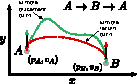
\includegraphics[width=0.4\textwidth]{../ch1/figures/robotcontrol_a.pdf}
\caption{Task description in the robotic manipulator example.\label{fig:ch1:robotcontrol_a}}
\end{figure}

% new paragraph
Consider a pick-and-place task shown in Fig.~\ref{fig:ch1:robotcontrol_a} (move an object from one place to another and return) that will be performed by a robotic manipulator (a device that can perform tasks without direct human interaction) \cite{Spong2005a}.
There are a number of ``robots'' that can perform such a task.
A few of these forms or architectures are shown in Fig.~\ref{fig:ch1:robotarch}.
Figure~\ref{fig:ch1:robotarch_a} displays a two-link serial architecture.
An alternative architecture could have an additional link placed in series as is shown in Fig.~\ref{fig:ch1:robotarch_b}.
Links can be combined in a variety of ways to create new architectures such as the four-link parallel manipulator in Fig.~\ref{fig:ch1:robotarch_c}.
Additional components or building blocks can be added to the architectures such as the triangular plate in Fig.~\ref{fig:ch1:robotarch_d}.
There are other decisions to be made with respect to the architecture including the joints that will be active (i.e.,~an actuator is present so a torque can be directly applied to the joint).
The potential actively actuated joints are represented by red arrows in Fig.~\ref{fig:ch1:robotarch}.
From this discussion, the essence of the architecture design decisions is the selection of the components and their connectivity.

\begin{figure}
\centering
\begin{subfigure}[t]{0.22\textwidth}
\centering
	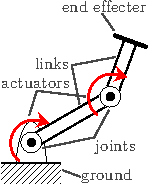
\includegraphics[scale=1]{../ch1/figures/robotarch_a.pdf}
    \caption{Two-link serial.\label{fig:ch1:robotarch_a}}
\end{subfigure}%
\begin{subfigure}[t]{0.22\textwidth}
\centering
	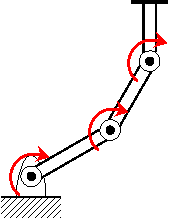
\includegraphics[scale=1]{../ch1/figures/robotarch_b.pdf}
    \caption{Three-link serial.\label{fig:ch1:robotarch_b}}
\end{subfigure}%
\begin{subfigure}[t]{0.25\textwidth}
\centering
	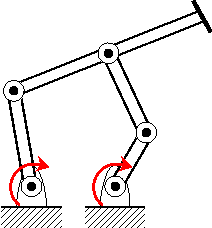
\includegraphics[scale=1]{../ch1/figures/robotarch_c.pdf}
    \caption{Four-link parallel.\label{fig:ch1:robotarch_c}}
\end{subfigure}%
\begin{subfigure}[t]{0.31\textwidth}
\centering
	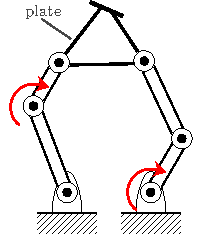
\includegraphics[scale=1]{../ch1/figures/robotarch_d.pdf}
    \caption{Four-link with a plate.\label{fig:ch1:robotarch_d}}
\end{subfigure}%
\caption[Some candidate robot manipulator architectures]{Some candidate robot manipulator architectures (red arrow indicates active joints).\label{fig:ch1:robotarch}}
\end{figure}

% new paragraph
Some potential plant design variables for this problem are shown in Fig.~\ref{fig:ch1:robotplant}.
The link length, cross-section geometry, and ground spacing are all geometric plant variables.
The spacing of the ground joints relative to point $A$ in Fig.~\ref{fig:ch1:robotcontrol_a} could also be considered plant variables.
All of these design variables are time-independent and related to the physical form of the manipulator.
The distribution of the plant variables can vary depending on the architecture considered.
If we use the two-link manipulator in Fig.~\ref{fig:ch1:robotarch_a}, then there will be only two length variables versus the four length variables associated with the four-link manipulator in Fig.~\ref{fig:ch1:robotarch_c}.

\begin{figure}
\centering
\begin{subfigure}[b]{0.33\textwidth}
\centering
	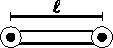
\includegraphics[height=0.5in]{../ch1/figures/robotplant_a.pdf}
    \caption{Link length.\label{fig:ch1:robotplant_a}}
\end{subfigure}%
\begin{subfigure}[b]{0.33\textwidth}
\centering
	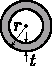
\includegraphics[height=0.7in]{../ch1/figures/robotplant_b.pdf}
    \caption{Cross-section geometry.\label{fig:ch1:robotplant_b}}
\end{subfigure}%
\begin{subfigure}[b]{0.33\textwidth}
\centering
	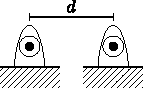
\includegraphics[height=0.8in]{../ch1/figures/robotplant_c.pdf}
    \caption{Ground spacing.\label{fig:ch1:robotplant_c}}
\end{subfigure}%
\caption{Plant variables in the robotic manipulator example.\label{fig:ch1:robotplant}}
\end{figure}

% new paragraph
The control design could involve the specification of the torque trajectories at the active joints such that the manipulator performs the pick-and-place task shown in Fig.~\ref{fig:ch1:robotcontrol_b}.
These are time-varying signals that could be chosen such that the minimum amount of time or energy is used.
The control design variables directly govern the behavior of the dynamic system.

\begin{figure}
\centering
	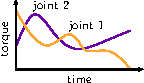
\includegraphics[width=0.35\textwidth]{../ch1/figures/robotcontrol_b.pdf}
    \caption{Joint control trajectories in the robotic manipulator example..\label{fig:ch1:robotcontrol_b}}
\end{figure}

% new paragraph
It is not uncommon for each design domain to be treated separately.
For example, the architecture may be assumed to be fixed while either the plant or control is developed.
Recent work has considered combined plant and control design and this system-focused approach led to low energy consumption solutions \cite{Allison2013d}.
Considering all three of the design domains could further lead to breakthroughs in performance and completely innovative systems.
There are some potential challenges with solving this design problem including the determination of what architectures to consider, developing models for each considered architecture, and solving an appropriate optimization problem for each architecture to properly evaluate its performance.

\section{Three Design Domains\label{sec:ch1:domains}}

In this section, we will discuss the classification of the three design domains.
The purpose of these classifications is to help conceptualize what can we change and how can we handle these decisions in system-level design.

%----------------------------------------------------------
\subsection{Architecture\label{sec:ch1:architecture}}

In the engineering design context, architecture is defined as the elements contained within a system and their relationships \cite{Crawley2004a}.
An architecture design problem seeks to optimize some performance measure subject to the necessary constraints by determining both the distribution of the elements and their relationships in the system.
A complementary use of the architecture representation is during the design process (see Sec.~\ref{sec:ch1:process}) where the elements and their relationships may change for reasons other than optimization of the system's performance.
The term ``element'' is a very generic but appropriate term as the elements in an architecture can be very different.
Some dissimilar types of architecture elements include:
\begin{itemize}[noitemsep]
\item Choosing between two elements with similar function but differing properties such as motor $A$ vs. motor $B$ from a manufacturer's catalog
\item Choosing elements with different functions such as a spring vs. a damper
\item Choosing elements with different assumptions/forms such as an active vs. semi-active actuator, or feedback controller vs. open-loop controller
\item Choosing elements with different levels of model fidelity such as a linear spring vs. a nonlinear, finite element-based spring
\end{itemize}

It is important to consider that not all architecture elements are meant to be strict design decisions.
For example, seeking the best performing architecture by varying elements with similar function but different levels of model fidelity is not particularly useful.
Therefore, a key point is that an architecture representation used during the design process does not need to be the final, realizable architecture to still be useful.
There are advantages in using different levels of design representation which will be discussed more in Sec.~\ref{sec:ch1:process}.
However, the broad definition of architecture used here encompasses the whole of an engineering system and its design representation.

% new paragraph
Component is a common alternative term for element (and will be used frequently throughout this dissertation).
Often, an architecture is made up of a particular set of components chosen from a set of discrete choices or a catalog.
Components in the catalog may be homogeneous (all the same) or heterogeneous (different).
The relationships between the elements of the architecture can be frequently captured by a graph \cite{Herber2017a}.
These relationships, or connections, could be physics-based or general information sharing.
From these definitions, we see that architecture design primarily involves the determination of discrete concepts (rather than the primarily continuous variables used in the remaining two design domains).

% other names
An alternative term for architecture is topology.
Topology more commonly refers to the connections between similar elements, while architecture tends to focus on the specifics.
For example, consider a series-parallel topology for an electrical circuit.
Traditionally, such a classification implies that replacing a particular component (e.g.,~swapping a capacitor for an inductor) in the circuit would still have the same topology.
There is even a particular element type that forgos the direct specification of the component known as the general impedance element. 
However, there are alternative definitions would classify these as different topologies.
Another domain where topology is frequently used is in structural optimization \cite{Bendsoe2004a, Lohan2016c}.
In these types of architecture design problems, the elements are typically homogeneous (e.g.,~all are bars in the truss with the same type of area shape), so it does fit the definition of the connections between similar elements.
Throughout this dissertation, both may still be used interchangeably even though this delineation between architecture and topology might be useful.

% examples
There are many architectures with heterogeneous components, such as electrical circuits \cite{Macmahon1994a, Lomnicki1972a, Isokawa2016a,manuscript-pm-circuits}, hybrid powertrains \cite{Bayrak2016a}, vehicle suspensions \cite{Herber2017a}, gear trains \cite{Pennestri2015a, Castillo2002a}, and biological networks \cite{Ma2009a} that are represented by colored graphs where the colors (or labels) are the component types.
There are a large number of geometric architecture problems such as the design of trusses \cite{Bendsoe2004a}, heat spreaders \cite{Lohan2016c}, and soft robotics \cite{Cheney2013a}.
These problems sometimes have homogeneous elements, but a few have heterogeneous elements such as in soft robotics where the material at different locations can have a different behavior \cite{Cheney2013a}.
Sometimes, the architecture problem can be approximated with a continuum relaxation, such as with the solid isotropic material with penalization algorithm for structural optimization \cite{Bendsoe2004a, Lohan2016c}.
However, the final solution still needs discrete values to define a realizable architecture.

%----------------------------------------------------------
\subsection{Plant\label{sec:ch1:plant}}

The plant design is defined by variables that are generally regarded as time independent.
Often this implies physical variables such as geometry, but may be other types such as spring stiffness (a lumped quantity).
Sometimes the distinction is made when comparing between control and plant. Plant (sometimes called the artifact in this domain) are the quantities fixed during the control design. 
For example, the variables that can modify the dynamic equations without any control present would represent the plant.

% new paragraph
Frequently, the variables are continuous scalars, but other types are possible. 
Examples of continuous scalars plant variables include the lengths of the links in a robotic manipulator \cite{Allison2013d} or the cross sectional area of truss elements \cite{Bendsoe2004a}.
The distributed thickness of a beam could be a part of the plant design (an infinite-dimensional plant variable) \cite{Chilan2017a}.
Discrete variables are also possible, such as the number of teeth in a gear \cite{Budynas2014a}.

%----------------------------------------------------------
\subsection{Control\label{sec:ch1:control}}

Control seeks to govern directly the behavior of a dynamic system, i.e.,~one which evolves through time.
Unlike the other two design domains, control is frequently considered more adjustable for different tasks or conditions, i.e.,~one system may have different control schemes for different scenarios.

Generally speaking, there are two types of control paradigms: closed loop and open loop.
In \glsfirst{CLC}, there is some type of feedback mechanism where the current state of the system is considered when making decisions about the next action to take.
In \glsfirst{OLC}, there is no feedback mechanism.
With no feedback mechanism, open-loop control design variables are typically entire trajectories.
An example of an OLC variable is the torque trajectory for a rotatory actuator in a robotic manipulator \cite{Allison2013d}.
For closed-loop control, gains or other variables that modify aspects of the feedback mechanism could be considered the control design.
An example of CLC is in the infinite-horizon linear-quadratic regulator with full state feedback \cite{Liberzon2012a}.

%----------------------------------------------------------
\subsection{Ambiguity in These Delineations\label{sec:ch1:}}

While descriptions were provided for each of the three design domains, there is still some ambiguity on how to provide the appropriate classifications.
There are a number of potential reasons for this vagueness.

% new paragraph, engineers
One of the primary reasons may simply be legacy design paradigms that treat certain parts of the design as separate \cite{Allison2014a}.
System engineers may tackle the architecture design while the mechanical and control engineers deal with the plant and control designs, respectively (and what is in their domain is decided by some form of management).
Therefore, the classification of the design variables may be along the lines of what is traditionally expected for the particular type of engineer to handle during the design process.
In a system-level design approach, as is preferred in this work, this type of classification is not needed as all domains are considered uniformly.

% new paragraph, optimization
Another type of delineation is based on variable types.
Architecture design variables are discrete.
The plant consists of continuous, time-independent variables and the control is infinite-dimensional trajectories.
This classification scheme has the advantage of utilizing techniques specifically created to handle each of the variable types.
However, the discussion above for each design domain demonstrated that the domains contain variables of variety types.
In a similar way, the general theory or tools may be developed to handle certain parts of the design domains which may provide their own classifications (e.g.,~multidisciplinary design frameworks \cite{Allison2014a}).

% new paragraph, approximations
Another difficulty comes when the approximations or better representations of design variables in one domain are frequently  classified in another domain.
Consider the following examples where a design decision in one domain is approximated in another design domain:
\begin{itemize}
\item Architecture $\to$ plant: the solid isotropic material with penalization approximation in structural optimization \cite{Bendsoe2004a, Lohan2016c}

\item Architecture $\to$ control: assuming a particular feedback controller form for the power take-off in wave energy conversion so that standard control-design techniques can be applied rather than selecting a specific power take-off architecture \cite{Falnes2002a}

\item Plant $\to$ architecture: using only preferred discrete component values in a circuit (e.g.,~E12 series) rather than continuous values for the inductance and capacitance \cite{Gan2010a}

\item Plant $\to$ control: abstracting the power take-off system in a wave energy converter to an open-loop force trajectory rather than a physical-system with plant variables \cite{Herber2013a, Herber2014a}

\item Control $\to$ plant: tuning a passive system with only physical components such as dampers and springs instead of a full-state feedback controller
\end{itemize}

\noindent In many of these cases, the designers may not put much importance in their classification but rather treat them as the necessary design variables for the problem at hand.

% new paragraph
A final point is the concept of plant and control architectures.
For new systems, it may be beneficial to split up the architecture decisions that are traditionally linked to the plant and control systems \cite{Deshmukh2015a}.
For example, candidate plant architectures for automotive
hybrid powertrains include series, parallel, and power-split, among others \cite{Bayrak2015a}.
For the power-split architecture (and other similar new architectures), the splitting of the power between the energy producing components is a necessary control decision \cite{Bayrak2015a}.
The specific controller used to make this control decision is the control architecture and may be an open-loop trajectory, a basic feedback controller, or any number of alternatives depending on the stage in the design process or its performance.

\section{A Design Process for Complete Dynamic System Design\label{sec:ch1:process}}

\begin{figure}
\centering
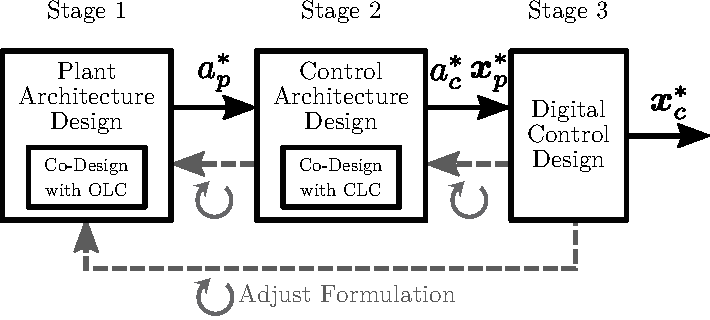
\includegraphics[width=0.6\textwidth]{../ch1/figures/stages2.pdf}
\caption{Proposed stages for complete dynamic system design.\label{fig:ch1:stages}}
\end{figure}

Allowing flexibility in all design domains can create a number of challenges that can limit how effectively one arrives at a suitable solution.
Here we adopt the design process proposed in Ref.~\cite{Deshmukh2015a} for complete dynamic system design that helps manage the complexity and uncertainty found in combined architecture, plant, and control design problems.
It is a three stage process shown in Fig.~\ref{fig:ch1:stages}.
We denote the plant architecture as $\glsfirst{architecture}_{\glsfirst{plant}}$ and associated plant variables as $\gls{x}_p$.
The control architecture is represented with $a_{\glsfirst{control}}$ and control variables $\bm{x}_c$ (and OLC variables as $\gls{olc}$).
The system-level objective function is represented by $\gls{objective}$.

% new paragraph
The first stage seeks to determine the optimal plant architecture by forgoing the specification of the control architecture.
Using a specific control architecture limits creative plant design exploration at early design stages \cite{Deshmukh2015a}.
Instead, OLC is used for the control among other potential uses.
OLC can replace some components or interfaces with optimal trajectories, reducing the design problem size while still providing an optimal solution \cite{Deshmukh2015a, Herber2014a, Allison2014b}.
In addition, OLC-based studies are particularly valuable at early design stages for gaining insights into upper system performance limits and dynamic behaviors and interactions that lead to system-optimal performance \cite{Allison2014a, Allison2013d,Son2010a, Schaala1993a, Mourik2009a, Karkee2010a}.
Furthermore, combined plant and control design, or co-design, will be used to determine the performance for each candidate plant architecture because it is a system-level optimization strategy \cite{Herber2017b, Fathy2003a, Allison2014a} that will allow fair comparisons between candidate plant architectures \cite{Bayrak2015a}.

\begin{figure}
\centering
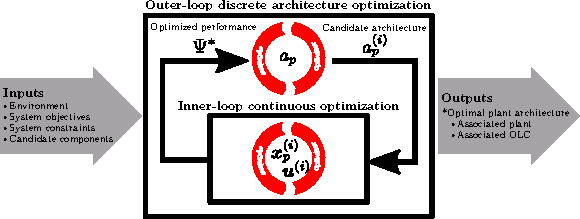
\includegraphics[width=0.8\textwidth]{../ch1/figures/outerinner2.pdf}
\caption{Stage 1 details.\label{fig:ch1:outerinner}}
\end{figure}

% new paragraph
The specifics for stage 1 are shown in Fig.~\ref{fig:ch1:outerinner}.
The inputs are the information about the system's operating environment, objectives, constraints, and a catalog of candidate components.
A nested optimization approach is used to handle the different variable types.
Here the outer loop will change the discrete (plant) architecture design variables while the inner loop determines the optimal performance by solving the continuous co-design problem for the candidate architecture. 

% new paragraph
Stage~2 in Fig.~\ref{fig:ch1:stages} seeks to determine the best control architecture given the optimized plant architecture from stage~1.
Similar to stage~1, a nested optimization approach can be used to vary the discrete control architecture decisions while the appropriate co-design problem is solved to determine the optimal performance for the candidate architecture.
For example, we could consider a basic feedback, hybrid \cite{Lygeros2008a}, or model predictive \cite{Borrelli2017a} controller architectures.
The final stage, stage~3, seeks to determine the digital controller design given the plant and controller architectures from the previous stages \cite{Landau2006a}.

% new paragraph
It might be necessary to iterate between the stages if unforeseen issues appear.
Information about these issues can be passed back to the previous stage and the problem formulation can be adjusted to address overlooked elements.
Additionally, in each of the stages, a sequence of problems may be posed and solved, each one informed by the results of the previous problem, moving toward greater levels of system specificity.

The theory and studies in this dissertation will primarily focus on design problems in stage~1, but it is important to understand the motivations behind these studies and how they fit into the entire design process.

%----------------------------------------------------------
\section{Solution Generation Challenges\label{sec:ch1:theorytools}}

There are a number of challenges associated with the design freedom found in combined architecture, plant, and control problems.
The complexity of individual problems can be quite significant, sometimes even rendering the problem intractable, unless this complexity is handled appropriately.  
Efficiently automating the key tasks in the solution generation process is essential to arriving at desirable solutions in a practical manner.
Here we highlight three important generation tasks: candidate architecture generation, model generation, and optimization problem generation.

%----------------------------------------------------------
\subsection{(Automated) Candidate Architecture Generation\label{sec:ch1:archgen}}

Exploring different architectures requires an appropriate conceptual framework that allows for modifications to the appropriate elements in the architecture.
A straightforward, commonly used representation is an adjacency matrix where the nonzero entries in the matrix represent connections between elements in the architecture.
Candidate architectures could be a different set of nonzero values in the adjacency matrix.
However, not all architecture representations are equally useful.
Some might produce many infeasible systems or too many candidates.
Others might produce many architectures with poor performance, or are not amendable to some optimization procedure.
An example alternative representation framework was developed for electrical circuits where a sequence of low-level instructions are used to generate a circuit \cite{Lohn1999a}.
These instructions iteratively add new elements to the circuit in  topologically different ways.
A manual alternative would include experts proposing candidate architectures, which may be appropriate in some cases, but often may not support comprehensive design space exploration.
In many traditional engineering design problems, the architecture is fixed so this abstract representation is not typically needed.

%----------------------------------------------------------
\subsection{(Automated) Model Generation\label{sec:ch1:modelgen}}

Given some architecture specification (e.g.,~a graph), we need to create a suitable model (some representation of the architecture that can predict performance and identify if constraints are satisfied) for use in the optimization problems described in Sec.~\ref{sec:ch1:process}.
Certain modeling methodologies support this task such as bond graph
modeling \cite{Borutzky2010a} or block diagram-based modeling \cite{matlab-simulink}. 
Other techniques have been developed for specific types of problems such as solid isotropic material with penalization for structural optimization \cite{Bendsoe2004a} and \glsfirst{MNA} for electrical circuits \cite{Ho1975a}.
Nevertheless, for many design problems, some investment will be needed to generate models efficiently and in an automated manner.
In traditional engineering design problems, the model is fixed for the given architecture, but can vary based on the plant/control design variables.

%----------------------------------------------------------
\subsection{(Automated) Optimization Problem Generation}

For different candidate architectures of the same design problem,  the optimization problem that predicts its performance may vary.
If the model is different, there may be different plant and control variables.
Different constraints may be present depending on the components in the architecture (e.g.,~we only need control actuator bounds if the component is present).
Since all problem elements (e.g.,~number and types of variables, objective function form, constraints, model) could change between architectures, forming and solving the optimization problem automatically is important for solution efficiency.
Understanding the general optimization problem structure for any candidate architecture is key so that it can be leveraged to find solutions faster and more robustly.
For some types of optimization problems, such as ones with infinite-dimensional constraints and variables, additional work is need to obtain (approximate) solutions.
Frequently, only a single optimization problem form needs to be posed and solved in traditional engineering design problems.

\section{Dissertation Overview\label{sec:ch1:overview}}

This introduction has provided a discussion on the combined architecture, plant, and control design problems including how this problem type can be used in the dynamic system design process and some potential challenges.
Due to the diverse design domains considered in this dissertation, a variety of methodologies are presented to manage different elements in the design process.
Chapters \ref{ch:2}--\ref{ch:5} focus on the development of these methodologies while Chapters \ref{ch:6}--\ref{ch:8} present detailed engineering design case studies that utilize the concepts.
A focus in the initial chapters is on the generality of the proposed approaches.
The frameworks presented are developed with specific consideration of what types of problems will fit under the proposed framework.

\begin{itemize}
% new paragraph, architecture
\item Chapter~\ref{ch:2} focuses on the task of representing and generating candidate architectures.
The theory and algorithms developed in this chapter are applicable to architecture problems where the architecture is representable by a colored graph built from a catalog of components.
A complete listing of all potential architectures under specific assumptions can be generated with this approach.
A number of enhancements to the algorithms presented in this chapter are detailed in Appendix~\ref{app:A}.

% new paragraph, co-design
\item Chapter~\ref{ch:3} focuses on a methodology for handling the other two design domains: combined plant and control design or co-design.
The general co-design problem formulation and optimality conditions are explained for both the simultaneous and nested solution strategies.
Due to a number of challenges associated with the optimality conditions, practical solution  considerations are discussed with a focus on the motivating reasons for using direct transcription in co-design.

% new paragraph, scaling
\item Chapter~\ref{ch:4} concentrates on scaling in dynamic optimization (a general class of problems found in Chapter~\ref{ch:3}). 
The necessary theory for scaling dynamic optimization formulations is presented and a number of motivating examples are shown. 
Scaling can be used to help facilitate finding accurate, generalizable, and intuitive information. The unique structure of dynamic optimization suggests that scaling can be utilized in novel ways to provide better analysis and formulations more favorable for efficiently generating the solution. 
A simpler, scaled problem is used to understand the general trends found in the results of the case study in Chapter~\ref{ch:7}, along with minor roles in the other two case studies.

% new paragraph, direct transcription
\item Chapter~\ref{ch:5} presents the direct transcription method for finding approximate solutions to dynamic optimization problems.
The method discretizes (in time) the infinite-dimensional quantities and creates a mathematical program that can be solved.
This method is an enabling method that allows solutions to be obtained for general co-design problems in Chapter~\ref{ch:4}.
A bulk of the chapter is focused on solving a particular subclass: linear-quadratic dynamic optimization problems.
These problems can be approximated with quadratic programs and be efficiently constructed and solved.
Problems with this structure are particularly important when the three domains are considered because many control problems may need to be solved, and an inefficient method could hinder the ability to explore the solutions.
The algorithms, sparsity patterns, and example codes are in Appendix~\ref{app:C}.
The case studies in Chapter \ref{ch:7} and \ref{ch:8} utilize this theory and codes to solve the control subproblem.

% new paragraph, passive analog circuits
\item Chapter~\ref{ch:6} presents an enumeration-based synthesis methodology for passive analog circuits by generating and evaluating all appropriate circuits.
Two design problems are considered: frequency response matching and low-pass filter realizability.
The circuit graphs (architectures) are generated using the methods described in Chapter~\ref{ch:2}.
This problem contains both architecture and plant design decisions.

% new paragraph, strain-actuated solar arrays
\item Chapter~\ref{ch:7} focuses on the design of strain-actuated solar arrays for spacecraft precision pointing and jitter reduction.
This problem has a variety of challenging plant and control design variables.
The nested co-design strategy described in Chapter~\ref{ch:3} is utilized, and the control subproblem is solved with the methods in Chapter~\ref{ch:5}.
The primary example from Chapter~\ref{ch:4} provides a number of insights into the results found in this case study.

% new paragraph, vehicle suspensions
\item Chapter~\ref{ch:8} is a case study that combines all three design domains with the design of vehicle suspensions.
The work from Chapters~\ref{ch:2}--\ref{ch:5} all contribute in addressing this complex design problem.
This chapter also includes a discussion of a general class of architecture, plant, and control design problems that utilize linear physical elements.

% new paragraph, conclusion
\item Chapter~\ref{ch:9} concludes the dissertation with an overall summary of the key points and identifies future research directions.

\end{itemize}

\begin{figure}[hb]
\centering
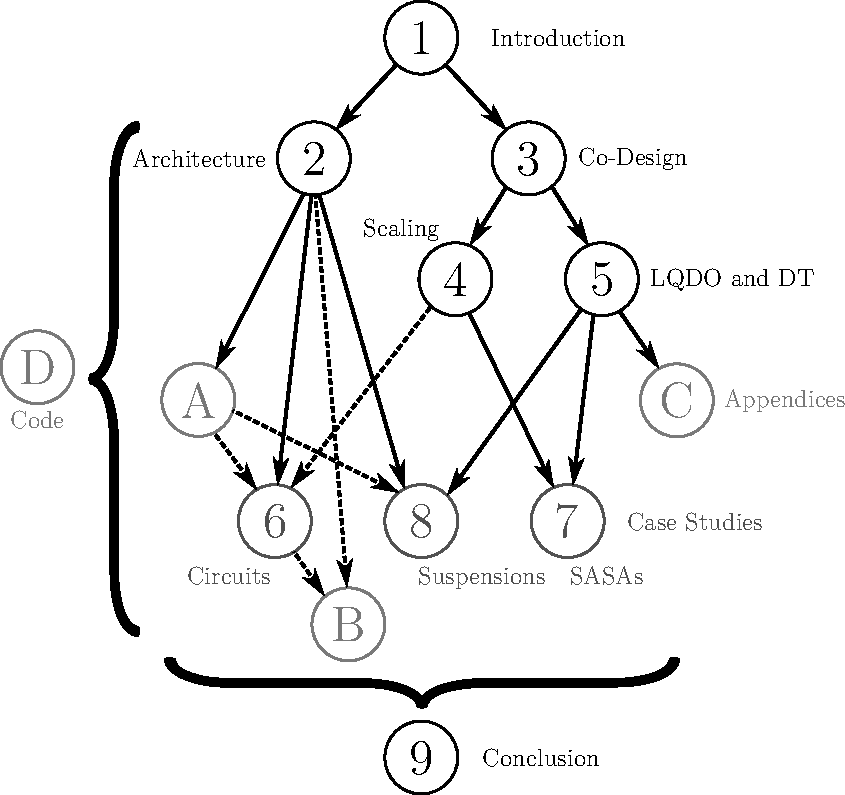
\includegraphics[width=0.65\textwidth]{../ch1/figures/outline2.pdf}
\caption[Dissertation content connections]{Dissertation content connections (dashed line indicates a narrower connection).\label{fig:ch1:outline}}
\end{figure} % introduction
\mychapterfoot{Candidate Architectures through Enumeration\label{ch:2}}

\footnotetext{Elements of this chapter are based on work completed in Ref.~\cite{Herber2017a, Herber2017d}.}

%--- epigraph
\epigraph{\textit{``Central to design is the creative act. This is not to imply that all needs are met creatively. Some are met by found solutions, found in handbooks, catalogues, department stores, etc. However, if a need is met through design, then creativity is involved.''}}{\textmd{R. A. Willem} \cite{Willem1990a}}
%--- epigraph

System architecture was defined as the elements or components contained within a system and their relationships in Sec.~\ref{sec:ch1:architecture} \cite{Crawley2004a, Mittal1989a, Wyatt2014a}. 
Designing breakthrough engineering systems with new capabilities and new levels of performance requires innovations in system architecture \cite{Cagan2005a, Chakrabarti2011a}.
Engineers often rely on heuristics such as design by analogy \cite{Chan2011a} and intuition when considering system architecture, but this may result in fixation on example designs and stifle innovation \cite{Linsey2010a}. 

Consider the following architecture design problem formulation:
\begin{subequations}
\label{eq:ch2:arch_outerloop}
\begin{align}
\min_{\bm{x}_a} \quad & \Psi(\bm{x}_a) \\
\text{subject to:} \quad & f_a(\bm{x}_a) = a \in \mathcal{F}_a
\end{align}
\end{subequations}

\noindent where $\gls{x}_{a}$ represents architecture design variables, $\gls{f}_a(\bm{x}_a)$ is a mapping between the architecture design variables and the architecture $\glsfoo[noindex]{architecture}$, and $\gls{objective}$ is a performance index. A fair comparison between architecture candidates in the set of feasible architectures $\gls{feasible}_a$ requires knowledge of the best possible performance for each candidate architecture. This requires optimization with respect to \textit{inner-loop} design variables such as plant and control design (see Chapter~\ref{ch:3}) \cite{Deshmukh2015a, Herber2017b}. The number design variables, constraints, models, etc.~can all change depending on the candidate architecture in the inner loop. Hence, formulating and solving architecture design problems can be challenging. Here we focus on a method that generates candidate architectures that may be used to determine the performance index with respect to an architecture-dependent inner-loop design problem.

Many studies have concentrated on effective representation and generation methods, primarily based on graph representations of the system architecture (see Fig.~\ref{fig:ch2:initialexamples} for some common engineering systems represented as graphs). There is a wide range of architecture design representations typically classified along the spectrum of continuum \cite{Hooshmand2012a, Khetan2015a} vs. discrete \cite{Munzer2013a, Guo2014a} design domains and homogeneous \cite{Hooshmand2012a, Khetan2015a} vs. heterogeneous \cite{Schmidt1997a, Munzer2013a} elements. The value of these methods often is to present new valid topologies to engineers for further evaluation (subjective or quantitative), helping to overcome design fixation. A popular class of methods for generating architecture candidates is generative representations \cite{Schmidt1997a, Schmidt2000a, Hornby2003a, Bryant2005a,  Hooshmand2012a,  Starling2005a, Chakrabarti2011a, Guo2014a}. This class covers a range of candidate architectures in an implicit form based on repeated application of rules that modify the graph. It has been recognized that generative approaches generate topologically simple designs, not covering the entire design space \cite{Munzer2013a}. Furthermore, the design space is sensitive to design knowledge \cite{Bryant2005a, Chan2011a} and rules \cite{Hooshmand2012a, Starling2005a}. While these designs may satisfy functional requirements elegantly, generation of more elaborate architectures is needed in some cases.

\begin{figure*}
\centering

\begin{subfigure}[b]{0.33\textwidth}
\centering
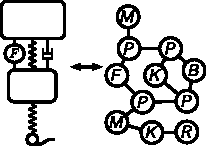
\includegraphics[scale=1]{../ch2/figures/suspension_optimized}
\caption{Suspension. \label{fig:ch2:initialexamples1}}
\end{subfigure}%
\begin{subfigure}[b]{0.33\textwidth}
\centering
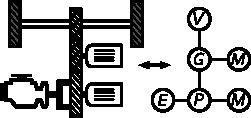
\includegraphics[scale=1]{../ch2/figures/powertrain_optimized}
\caption{Hybrid powertrain. \label{fig:ch2:initialexamples2}}
\end{subfigure}%
\begin{subfigure}[b]{0.33\textwidth}
\centering
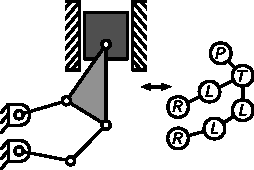
\includegraphics[scale=1]{../ch2/figures/linkage_optimized}
\caption{Mechanism. \label{fig:ch2:initialexamples3}}
\end{subfigure}

\vspace{0.05in}

\begin{subfigure}[b]{0.6\textwidth}
\centering
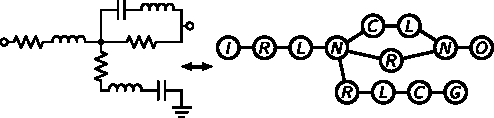
\includegraphics[scale=1]{../ch2/figures/circuit}
\caption{Electrical circuit.\label{fig:ch2:initialexamples4}}
\end{subfigure}%
\begin{subfigure}[b]{0.4\textwidth}
\centering
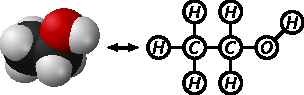
\includegraphics[scale=1]{../ch2/figures/molecule2}
\caption{Molecule.\label{fig:ch2:initialexamples5}}
\end{subfigure}

\caption{Architectures represented as graphs.\label{fig:ch2:initialexamples}}

\end{figure*}

It can be challenging to describe the design space of an architecture generation method, partially due to the combinatorial nature of architecture design problems. A better understanding of how certain rules restrict the design space can lead to better generative approaches, but this requires a complete design space to compare against. Furthermore, the ultimate goal is a set of all architectures that are feasible with respect to constraints \cite{Wyatt2012a} and that are unique \cite{Schmidt2000a}.  Arriving at such a design space efficiently is a considerable challenge.

In this chapter, the design space is completely captured by a perfect matchings approach for a certain class of architecture design problems, more specifically, problems that are represented by undirected colored graphs under the component/port paradigm \cite{Mittal1989a, Snavely1993a, Munzer2013a}.
The proposed approach generates truly novel architectures (in fact all of them) but still leverages some of the natural constraints found in architecture design problems to reduce the number of graphs generated.
This design space is found through an enumeration, i.e., a complete, ordered listing of all the items in the collection of feasible and unique architectures.
This approach leads to a number of interesting insights into the fundamental nature of architecture design problems.

The remainder of the chapter is organized as follows.
The next section outlines the some of the basic theory behind candidate architectures with perfect matchings.
Network structure constraints and the colored graph isomorphism problem are then discussed, with the objective of achieving feasible unique architectures.
Using the insights from the previous two sections, a tree search algorithm is developed that more efficiently covers the same design space.
A number of case studies are then presented.
Finally, a discussion is given of the results and how the proposed approaches can be used in current architecture design research.

%------------------
\section{Candidate Architectures with Perfect Matchings \label{sec:ch2:candidates}}

First, some relevant graph theory background is given.

\begin{definition}[Graph] \label{def:ch2:graph}
A graph is a pair $\gls{G} = (\gls{V},\gls{E})$ of sets satisfying $E \subset [V]^2$ where the elements of $V$ are the vertices and the elements of $E$ are its edges. 
\end{definition}

A \textit{simple graph} is an unweighted, undirected graph containing no graph loops or multiple edges. 
The adjacency matrix of $G$ is the $\gls{number} \times n$ matrix \gls{A}$\ = A(G)$ whose entries $a_{ij}$ are given by:
\begin{align*}
a_{ij} = \begin{cases}
1 & \text{if the set $(v_i, v_j) \in E$} \\
0 & \text{otherwise} \\
\end{cases}
\end{align*}

\noindent For a simple graph, the \textit{adjacency matrix} must have 0s on the diagonal. For an undirected graph, the adjacency matrix is symmetric and if only a subset of the edges are present in $E$, the correct $A(G)$ can be constructed with $\mathrm{sign}(A + A^{\gls{transpose}})$. The \textit{connectivity matrix} of simple graph $G$ can be found with:
\begin{align} \label{eq:ch2:connectivity}
A_{\glsfirst{component}}(n) =  A^n
\end{align}

\noindent where the interpretation of $A_C(n)$ is for every nonzero entry, there exists at most $n$ undirected walks required to go from $v_i$ to $v_j$, i.e.,~the pair of vertices are connected in some sense \cite[p.~165]{Godsil2001a}. We will assume that $n$ is the same as the length of $A$ giving all walks. 

The degree of a vertex is the number of edges incident at the vertex and the average degree is $\gls{d} = 2 \abs*{E} / \abs*{V}$ \cite[p.~5]{Diestel2000a}. A \textit{matching} in a graph is a set of edges such that no two have a vertex in common and a perfect matching is a matching that covers every vertex \cite[p.~255]{Rispoli2007a}.

\begin{definition}[Colored Graph] \label{def:ch2:cgraph}
A colored graph $G$ is a three-tuple $(V,E,L)$ where $(V,E)$ specifies an undirected graph and $\gls{L}=\{V_i\}^k_{i=1}$ is a partition of the vertices into color sets ($V_i \cap V_j = \Phi$, $i \neq j$, and $(\cup_{i=1}^k V_i) = V$). For convenience, define $\mathrm{color}(v) = i$ if $v\in V_i$.
\end{definition}

The graphs in Fig.~\ref{fig:ch2:initialexamples} are colored graphs where each vertex represents a component. The colored labels indicate different component types. For example, in Fig.~\ref{fig:ch2:initialexamples}a, \circled{\xcolor{K}} represents a vertex with a coloring $\gls{colorings}$ indicating that it is a spring component type and that \circled{\xcolor{B}} represents a damper component type. These are termed 2-\textit{port} components since they can have up to 2 unique edges if ports are connected to a single additional vertex (this port notion is analogous to bond graph modeling \cite{Wu2008a}).
However, there are fundamental limitations with this representation. For example, 
if the order that the ports of a component are connected to edges prescribed in $A$ is important, then pure component graph representation is not sufficient for determining a unique architecture. Consider the planetary gear \circled{\xcolor{P}} in Fig.~\ref{fig:ch2:initialexamples}b. Since the planetary gear is represented by a single vertex, it is unclear which of the connected components \{\circled{\xcolor{E}}, \circled{\xcolor{G}}, \circled{\xcolor{M}}\} is connected to the sun, ring, and carrier (common names for the planetary gear ports \cite{Bayrak2016a}). Permutations of this decision would result in different architectures but the same adjacency matrix. Another limitation is the unspecified nature of parallel connections when only component-level vertices are used. If the adjacency matrix specifies that $\xcolor{K}$ has three connections, it cannot be necessarily uniquely determined what connections are incident at each specific port of $\xcolor{K}$. A better representation would determine unique graphs, motivating a pure ports graph representation of architectures.

%------------------
\subsection{Ports Graph}

A port graph $G^{\gls{port}}$ is constructed from a three-tuple $({C},{R},{P})$: 
\begin{enumerate}[label=$\bullet$, leftmargin=*, widest=$\bullet$, nosep]

\item $\gls{C}$ is the colored label set representing distinct component types, whose size is denoted by $n_C$

\item $\gls{R}$ is a column vector indicating the number of replicates for each component type

\item $\gls{P}$ is a column vector indicating the number of ports for each component type
\end{enumerate}

Using $({C},{R},{P})$ we will create the three-tuple $({V},{E},{L})$ that defines a proper colored graph (see Definition~\ref{def:ch2:cgraph}). The definition of an $n$-port component in this context is all $n$ ports are completely connected to each other. Therefore each component can be considered a complete graph of its ports (see Fig.~\ref{fig:completegraphs} for the first five complete graphs). The vertex and edge set for $G^{P}$ is then defined as the union of these complete subgraphs:
\begin{align}
({V},{E})^{P} = \bigcup_{k=1}^{n_C} \bigcup_{j=1}^{R_k} K_{P_k}
\end{align}

\noindent where $\gls{K}_{P_k}$ is a complete graph of size $P_k$.

\begin{figure}
\centering

\newcommand{\completegraphssize}{1in}

\tikzsetnextfilename{completegraphs}

\resizebox{\completegraphssize}{!}{
\begin{tikzpicture}
\node () at (-1.3,-1.3) {};
\node () at (1.3,-1.3) {};
\node () at (-1.3,1.3) {};
\node () at (1.3,1.3) {};
\node () at (0,-1.6) {\Large $K_1$};
\graph { subgraph K_n [n=1, counterclockwise, nodes={very thick,circle,draw,inner sep=1pt,minimum size=1pt}, edges={black, very thick}] };
\end{tikzpicture}
}
%
\resizebox{\completegraphssize}{!}{
\begin{tikzpicture}
\node () at (-1.3,-1.3) {};
\node () at (1.3,-1.3) {};
\node () at (-1.3,1.3) {};
\node () at (1.3,1.3) {};
\node () at (0,-1.6) {\Large $K_2$};
\graph { subgraph K_n [n=2, counterclockwise, nodes={very thick,circle,draw,inner sep=1pt,minimum size=1pt}, edges={black, very thick}] };
\end{tikzpicture}
}
%
\resizebox{\completegraphssize}{!}{
\begin{tikzpicture}
\node () at (-1.3,-1.3) {};
\node () at (1.3,-1.3) {};
\node () at (-1.3,1.3) {};
\node () at (1.3,1.3) {};
\node () at (0,-1.6) {\Large $K_3$};
\graph { subgraph K_n [n=3, counterclockwise, nodes={very thick,circle,draw,inner sep=1pt,minimum size=1pt}, edges={black, very thick}] };
\end{tikzpicture}
}
%
\resizebox{\completegraphssize}{!}{
\begin{tikzpicture}
\node () at (-1.3,-1.3) {};
\node () at (1.3,-1.3) {};
\node () at (-1.3,1.3) {};
\node () at (1.3,1.3) {};
\node () at (0,-1.6) {\Large $K_4$};
\graph { subgraph K_n [n=4, counterclockwise, nodes={very thick,circle,draw,inner sep=1pt,minimum size=1pt}, edges={black, very thick}] };
\end{tikzpicture}
}
%
\resizebox{\completegraphssize}{!}{
\begin{tikzpicture}
\node () at (-1.3,-1.3) {};
\node () at (1.3,-1.3) {};
\node () at (-1.3,1.3) {};
\node () at (1.3,1.3) {};
\node () at (0,-1.6) {\Large $K_5$};
\graph { subgraph K_n [n=5, counterclockwise, nodes={very thick,circle,draw,inner sep=1pt,minimum size=1pt}, edges={black, very thick}] };
\end{tikzpicture}
}
%
%\resizebox{\completegraphssize}{!}{
%\begin{tikzpicture}
%\node () at (-1.3,-1.3) {};
%\node () at (1.3,-1.3) {};
%\node () at (-1.3,1.3) {};
%\node () at (1.3,1.3) {};
%\node () at (0,-1.6) {$K_6$};
%\graph { subgraph K_n [n=6, counterclockwise, nodes={very thick,circle,draw,inner sep=1pt,minimum size=1pt}, edges={black, very thick}] };
%\end{tikzpicture}
%}
%

%\caption{Complete graphs on $n$ vertices, for $n$ between 1 and 6. \label{fig:completegraphs}}
\caption{Complete graphs on $n$ vertices between 1 and 5. \label{fig:completegraphs}}


\end{figure}



The complete label for each vertex is constructed from a naming scheme where the base is the colored label from ${C}$, the subscript is the replicate number, and the superscript is the port number. Then the set of colored labels for $G^{P}$ can be constructed as:
\begin{align}
{L}^{P} = \bigcup_{k=1}^{n_C} \bigcup_{j=1}^{R_k} \bigcup_{i=1}^{P_k} \left\lbrace (C_k)_j^i \right\rbrace
\end{align}
\noindent where each label is unique at this point.

There are a number of graph measures and metrics that can be computed for this class of graphs. First, the number of vertices is given by: $N_P = \abs{{V}^{P}} = {P}\tran {R}$, where $\gls{abs}$ is the cardinality of a set. The number of edges in $K_n$ is $n(n-1)/2$ \cite[p.~22]{Godsil2001a}, so we can easily calculate the number of edges in $G^{P}$ as:
\begin{align}
\abs*{{E}^{P}} = \frac{1}{2} \left( {P}  \circ \left( {P} - 1 \right) \right)\tran {R}
\end{align}

\noindent where $\gls{hadamard}$ denotes the Hadamard product. The total number of components is: $N_C = e\tran {R}$ where $\gls{e}$ is a column vector of ones of appropriate length.

\subsection{Interconnectivity Graph\label{sec:ch2:inter}}

The essence of an architecture design problem is determining the relationships between ports. Therefore a natural question is: what are all the possible architectures? Subgraph enumeration provides a relevant framework for determining all possible graphs satisfying specified properties \cite{Rispoli2007a}. We now say that a candidate architecture in an architecture design space described by $(C,R,P)$ has the following properties:
\begin{enumerate}[nosep]
\item A set of components bounded by $(C,R,P)$ (so $n_P \leq N_P$, where $n_P$ is the total number of ports for the candidate architecture).
\item Each port in $(V^P, \{\ \}, L^P )$, i.e.,~$G^P$ without edges, is connected to another port (this implies $n_P$ is even and is also known as a complete topology since there are no open ports \cite{Snavely1993a}).
\end{enumerate}

\noindent Now, a complete architecture design space described by $(C,R,P)$ would be a set of candidate architectures that contain all possible valid subsets of components and all possible valid edge combinations between said subset of components. We will denote this graph structure space (a set of all graphs that fulfill a certain set of conditions) as $\glsfirst{gss}_1$. We will now see that the enumeration based on \glsfirstplural{PM} will correspond to the complete architecture design space.

Recall that a \mypm{} is a matching in which every vertex of the graph is incident to exactly one edge \cite{Rispoli2007a}; all \mypm{}s for $K_2$, $K_4$, and $K_6$ are shown in Fig.~\ref{fig:ch2:perfectmatchings}. Since a necessary condition for a \mypm{} is an even number of vertices, we will assume $N_P$ is even (Sec.~\ref{sec:ch2:comparison} discusses the implications of this restriction).  The number of \mypm{}s for $K_{n}$ can be calculated using the double factorial function:
\begin{align}
% \mathcal{D}(n)
\gls{doublefac} = (n-1)!! = (n-1) \times (n - 3) \times \dots \times 3 \times 1 \quad n \text{ even}
\end{align}
\noindent and the first several values of this function are $\mathcal{D}(2) = 1$, $\mathcal{D}(4) = 3$, $\mathcal{D}(6) = 15$, $\mathcal{D}(8) = 105$, $\mathcal{D}(10) = 945$, $\mathcal{D}(12) = 10,395$,  $\mathcal{D}(14) = 135,135$, $\mathcal{D}(16) = 2,027,025$, $\mathcal{D}(18) = 34,459,425$ \cite{OEISA001147}. This function grows slower than the traditional factorial function since the even elements have been omitted. This result agrees quite well with the bound by Mittal and Frayman for a similar problem (the bound being on order of $\sqrt{N_P!}$) \cite{Mittal1989a}.

\begin{figure}
\centering

\begin{subfigure}[b]{\columnwidth}
\centering
\input{../ch2/figures/perfectmatchings2}
\caption{$1!!$ perfect matchings for $K_2$.}
\end{subfigure}%

\begin{subfigure}[b]{\columnwidth}
\centering
\input{../ch2/figures/perfectmatchings4}
\caption{$3!!$ perfect matchings for $K_4$. \label{fig:pmthree}}
\end{subfigure}%

\begin{subfigure}[b]{\columnwidth}
\centering
\input{../ch2/figures/perfectmatchings6}
\caption{$5!!$ perfect matchings for $K_6$.}
\end{subfigure}%

\caption{Perfect matchings for $K_2$, $K_4$, and $K_6$.\label{fig:ch2:perfectmatchings}}

\end{figure}

For $n$ between $1$ and $\mathcal{D}(N_P)$, $\gls{pmedge}(n,N_P)$ denotes the edge set for the $n$th \mypm{} of $K_{N_P}$. The uniqueness of each \mypm{} can be ensured by ordering all edges with the first element being the larger vertex (in the sense of the index value). For example for the first graph in Fig.~\ref{fig:ch2:perfectmatchings}b, $\mathcal{P}(1,4) = \{ (4,1),(3,2) \} \neq \{ (1,4),(2,3) \}$. It will be convenient to map the edge set to a vector where sequential pairs are a single edge (e.g.,~$\{ (4,1),(3,2) \} \to [4\ 1\ 3\ 2]$. There are two interesting properties of the set of all \mypm{}s \cite{Rispoli2007a}:
\begin{enumerate}[nosep]
\item Enumerating all \mypm{}s of $K_N$ results in a set of graphs where all possible edge combinations are present where each port is connected to exactly one other port.
\item The set of \mypm{}s graphs of $K_N$, contains all edge sets for $K_{N-2}$, where $N \geq 4$.
\end{enumerate}

\noindent Now with these two properties in mind, consider any candidate architecture defined by the properties above. It has $n_P \leq N_P$ and $n_P$ is even, so there exists a \mypm{} matching edge set in the set of \mypm{} graphs of $K_{N_P}$ that contains the subset of components and the particular edge combination since all edge combinations of $n_P$ are found in the set $N_P$. Therefore, because any candidate architecture can be found in the set of \mypm{} graphs of $K_{N_P}$, a PM approach captures the complete architecture design space.

A \mypm{} approach is a type of \glsfirst{GNRS} since there is a binary relation between $\mathcal{G}_1$ and $n \in [1, \mathcal{D}(N_p)]$. A \mypm{} approach is {left-total} and {left-unique} with respect to complete topologies of $(C,R,P)$ (left implies a map from $\mathcal{G}_1$ to $n$ and these are desired properties for a GNRS) \cite{Wyatt2014a}. Algorithm~\ref{alg:ch2:singlepm} is useful for this direction as it determines $\mathcal{P}(n,N_P)$ \cite{github-pm-architectures-project, Rispoli2007a}\footnote{Ref.~\cite{github-pm-architectures-project} contains \textsc{Matlab} codes for Alg.~\ref{alg:ch2:singlepm} and more efficient recursive algorithm when all perfect matchings are required.
}. In addition, a \mypm{} approach is {right-total} and {right-unique} with respect to the same conditions (right implies a map from $n$ to $\mathcal{G}_1$). Algorithm~\ref{alg:ch2:inversepm} is useful for the right direction as it determines $\mathcal{P}^{-1}(E)$ where $E$ is a valid \mypm{} edge set. Based on these two efficient algorithms, a \mypm{} approach is \textit{algorithmic} in both directions \cite{Wyatt2014a}.

The interconnectivity graph $G^{\gls{interconnectivity}}$ then is defined with $V^P$, $L^P$, and an edge set from the set of \mypm{}s:
\begin{align} \label{eq:ch2:Ppm}
E^I = \mathcal{P}(n,N_P) \qquad \text{where $n \in \left[ 1, 2, \dots, \mathcal{D}(N_P) \right]$}
\end{align}

\noindent The number of edges is: $\abs{E^I} = N_P/2$.

% \IncMargin{1em}
\RestyleAlgo{algoruled}

\begin{vAlgorithm}[t]{\textwidth}{0em}

\LinesNumbered
\SetSideCommentRight 
\DontPrintSemicolon
% \SetNoFillComment

% \SetTitleSty{\textsf}{small}
% \renewcommand{\algorithmcfname}{\small\textbf{\textsf{\MakeUppercase{Algorithm}}}}%

% \SetKwData{Left}{left}\SetKwData{This}{this}\SetKwData{Up}{up}
\SetKwFunction{cumprod}{cumprod}
\SetKwFunction{length}{length}
\SetKwFunction{zeros}{zeros}
\SetKwFunction{ceil}{ceil}

\SetKwInOut{Input}{Input}
\SetKwInOut{Output}{Output}

\caption{Creation of edge set for a specific perfect matching number. \label{alg:ch2:singlepm}}

\Input{$\xvar{N}$  -- number of vertices (should be even) \\ $\xvar{I}$ -- perfect matching number, integer between 1 and $(\xvar{N}-1)!!$}
\Output{$\xvar{E}$ -- vector of edges in sequential pairs}
\BlankLine
    
	\glsfirst{variable}

   $\xvar{J}$ $\leftarrow$ $\big[ 1,3,5,\dots,\xvar{N}-1 \big]$ \tcc*{odd numbers from 1 to N-1}
   
   $\xvar{P}$ $\leftarrow$ $\big[ 1 , \cumprod(\xvar{J}) \big]$ \tcc*{cumulative double factorial}
    
   $\xvar{V}$ $\leftarrow$ $\big[ 1,2,\dots,\xvar{N}\big]$ \tcc*{create initial list of available vertices}
    
%    $\xvar{A}$ $\leftarrow$ $\zeros(1,\xvar{N})$ \tcc*{initialize output matrix}

        
		\For{$\xvar{j}\leftarrow$ $\xvar{J}$ }{
		
		    $\xvar{q}$ $\leftarrow$ $(\xvar{N}+1-\xvar{j})/2$ \tcc*{index for 2nd to last entry in P}
		           
            $\xvar{I}$ $\leftarrow$ $\ceil\big(\xvar{I}/\xvar{P}(\xvar{q})\big)$ \tcc*{calculate smaller vertex index}
            
            $\xvar{E}(\xvar{j})$ $\leftarrow$ $\xvar{v}(\xvar{end})$ \tcc*{assign largest remaining value}
            
            \text{remove element} $\xvar{V}(\xvar{end})$ \tcc*{remove largest remaining value}
            
            $\xvar{E}(\xvar{j}+1)$ $\leftarrow$ $\xvar{V}(\xvar{i})$ \tcc*{assign smaller selected value}
            
            \text{remove element} $\xvar{V}(\xvar{i})$ \tcc*{remove the smaller selected value}
            
            $\xvar{I}$ $\leftarrow$ $\xvar{I} - \big( (\xvar{i} - 1) \times \xvar{P} (\xvar{q}) \big)$ \tcc*{get index in subgraph with 2 vertices removed}
		
		
	} % end for j

	% $\xvar{A}(\xvar{N}-1)$  $\leftarrow$ $\xvar{V}(\xvar{end})$  \tcc*{final entries}
	
	% $\xvar{A}(\xvar{N})$  $\leftarrow$ $\xvar{V}(1)$
		
\end{vAlgorithm}

% \IncMargin{1em}
\RestyleAlgo{algoruled}

\begin{vAlgorithm}[t]{\columnwidth}{0em}

\LinesNumbered
\SetSideCommentRight 
\DontPrintSemicolon
% \SetNoFillComment

% \SetTitleSty{\textsf}{small}
% \renewcommand{\algorithmcfname}{\small\textbf{\textsf{\MakeUppercase{Algorithm}}}}%

% \SetKwData{Left}{left}\SetKwData{This}{this}\SetKwData{Up}{up}
\SetKwFunction{cumprod}{cumprod}
\SetKwFunction{length}{length}
\SetKwFunction{zeros}{zeros}
\SetKwFunction{ceil}{ceil}

\SetKwInOut{Input}{Input}
\SetKwInOut{Output}{Output}

\caption{Determination of the perfect matching number for a specific edge set. \label{alg:ch2:inversepm}}

\Input{$\xvar{E}$ -- vector of edges in sequential pairs, should be properly ordered and even length}
\Output{$\xvar{I}$ -- perfect matching number, integer between 1 and $(\xvar{N}-1)!!$}
\BlankLine
   
	$\xvar{N}$ $\leftarrow$ $\length(\xvar{E})$ \tcc*{total number of vertices}
	
	$\xvar{P}$ $\leftarrow$ \text{reverse elements of} $\cumprod( [1,3,5,\cdots \xvar{N}-3 ] )$  \tcc*{array flip, cumulative double factorial}
	
	$\xvar{V}$ $\leftarrow$ $\big[ 1,2,\dots,\xvar{N}\big]$ \tcc*{create initial list of available vertices}

    $\xvar{I}$ $\leftarrow$ $1$ \tcc*{initialize perfect matching index}
    

    
	\For{$\xvar{j}\leftarrow$ $1$ \KwTo $\xvar{N}/2-1$ }{
	
	
		$\xvar{q}$  $\leftarrow$ 	$\xvar{E}\big( 2 \xvar{j} - 1 \big)$ \tcc*{index of largest remaining vertex}

        $\xvar{V}( \xvar{q} )$ $\leftarrow$ $0$ \tcc*{zero entry, removing it}
        
       $\xvar{i}$ $\leftarrow$ \text{find index of $\xvar{E}(2\xvar{j})$ in the vector of nonzero elements of $\xvar{V}$} % \tcc*{i.e. V has 0s removed}
        
       %  $\xvar{i}$ $\leftarrow$ find(nonzeros(V)==E(2*\xvar{j})) \tcc*{return first (and only) entry}
        
        $\xvar{V}\big(\xvar{E}(2 \xvar{j}) \big)$ $\leftarrow$ $0$ \tcc*{zero entry, removing it}
        
        $\xvar{I}$ $\leftarrow$ $\xvar{I} + \big( (\xvar{i}-1)\times \xvar{P}(\xvar{j}) \big)$ \tcc*{sum to get build up the index}
	
		
	} % end for j 

\end{vAlgorithm}

\subsection{Connected Ports/Components Graph}

The connected ports graph is the union of the ports graph and interconnectivity graph:
\begin{align}
G^{\gls{CP}}  = G^P \cup G^I
\end{align}

\noindent The number of vertices is still $N_p$. There is possibility of multiple edges when combining the graphs since edges between the already connected ports of a component may be connected with a \mypm{}. We can simplify $G^{CP}$ by combining all multiple edges into a single equivalent edge, thus creating a simple graph. Using this operation, the number of edges of $G^{CP}$ can be bounded by:
\begin{align}
\abs*{E^P} \leq \abs*{E^{CP}} \leq \abs*{E^P} + \abs*{E^I}
\end{align}

\noindent since each edge of $E^I$ could be a repeat of an edge in $E^P$. $G^{CP}$ is a unique representation of an architecture since a \mypm{} is between specific ports and all components are fully connected subgraphs. 

There are advantages of the component graph representation that should be utilized, such as a reduced number of vertices and edges (and not differentiating replicates). We now characterize \textit{simple components} whose port ordering does not matter (e.g.,~a 2-port spring) and \textit{structured components} where it does (e.g.,~a 3-port planetary gear). All simple components will be reduced to a single vertex and the appropriate edges will be created. The labels for simple components will be modified by removing both the superscript and subscript of $L^{CP}$. Structured components will only have their subscripts removed to maintain port discernibility. This graph representation is termed the connected component graph $G^{\glsfirst{CC}}$.

To get a better sense of the structure of $G^{CC}$ consider all components to be simple components. Then the number of vertices is simply $N_C$. The number of edges of $G^{CC}$ can be bounded by $0 \leq \abs{E^{CC}} \leq \abs{E^I}$ and the labels are:
\begin{align}
{L}^{CC} = \bigcup_{k=1}^{n_C} \bigcup_{j=1}^{R_k} \left\lbrace C_k \right\rbrace
\end{align}

\noindent All graphs in the remaining sections are considered to be $G^{CC}$ graphs unless otherwise noted.

\section{Candidate Graphs to Unique Useful Graphs}

In the previous section an approach for enumerating architectures based on the consideration of every potential \mypm{} was outlined. However, there are a number of deficiencies in this set of architectures, including infeasible graphs based on practical constraints for a specific architecture design problem, and repeated graphs in the modeling sense. The following two subsections address architecture feasibility and uniqueness, respectively.

\subsection{Network Structure Constraints\label{sec:ch2:NSC}}

We define feasibility as a candidate architecture's satisfaction of all \glsfirstplural{NSC} for a particular architecture design problem. Similar to the rules in generative design approaches, the creation of the set of network structure constraints for a particular architecture design problem is subject to the creativity and intuition of the designer. Some of these constraints may be fairly self-evident while others might be vague or contentious (Ref.~\cite{Wyatt2012a} discusses these issues). Wyatt et al. describe four types of NSCs that are sufficient to define almost all aspects of realizability of an architecture and are summarized briefly (without edge coloring considerations) as \cite{Wyatt2012a}:
\begin{enumerate}[label=$\bullet$, widest=$\bullet$, nosep]
\item \Glsfirstplural{CNC} prescribe how many components of a given type must be present
\item \Glsfirstplural{DCC} prescribe which component types may be connected together by which connection types and cardinality of the connections
\item \Glsfirstplural{FOC} prescribe how many connections that components of a certain type must have in total
\item \Glsfirstplural{ICC} prescribe how many continuous paths there must be from every component of one type to every component of another type
\end{enumerate}

Graph generating algorithms designed to always satisfy certain NSCs could be more useful since all of the generated graphs would be feasible with respect to those certain NSCs.
Furthermore, graph generating algorithms can also be designed to produce graphs that have a higher proportion that satisfies certain NSCs than more naive approaches.
Some of the NCSs that are not satisfied can be with edits to the graph.
The only operation that will be considered here is the removal of vertices $G^{CC}$ and the corresponding edges and labels as it will maintain certain properties of the graph structure space $\mathcal{G}_1$.
Other operations such as vertex insertion, edge insertion, or label substitution destroy the analysis of the design space coverage that is possible with an enumerative \mypm{} approach.
Next, several common NSCs (denoted with \gls{S}) are described along with the specifics of checking their satisfaction with available graph analysis tools.

\begin{enumerate}[label=$S_{\!\arabic*}$]

\item \label{ch2:s1} Every graph must be a connected graph (ICC). A graph is termed connected if there is a path from any vertex to any other vertex in the graph \cite[p.~18]{Diestel2000a}. This can be checked with the connectivity matrix, $A_C(G)$, in Eqn.~(\ref{eq:ch2:connectivity}). If all entries in this matrix are not 1, then the graph is not connected.

\item \label{ch2:s2} Every graph can only have a maximum number of a given component type (CNC). This is defined by $R$ in the architecture definition three-tuple so is naturally handled by a \mypm{} approach. An example: `Every suspension must have less than 3 springs'.

\item \label{ch2:s3} Every graph must have a specific number of certain component types (CNC). These mandatory components will be captured with a vector \gls{M} of length $n_C$. The elements of $M$ are binary with a $1$ indicating all replicates of the component type must be present in the graph. An example: `Every hybrid powertrain must have an engine and a vehicle'.

\item \label{ch2:s4} Every graph must have specific component types connected to each other (ICC). This can be checked with the connectivity matrix in Eqn.~(\ref{eq:ch2:connectivity}). If nonzeros are not present at every location where a path must exist between component types, then the graph is infeasible. If we require \ref{ch2:s1} and \ref{ch2:s3}, then we can leverage the vector $M$ in \ref{ch2:s3} to satisfy both constraints by checking $A_C(G)$ such that all mandatory components are connected to each other. An example: `Every hybrid powertrain must have an engine connected to a vehicle'.

\item \label{ch2:s6} Every graph must have vertices whose number of unique edges is within a specific range (FOC). The values in $P$ can define the upper bound for each vertex since components are defined by a certain number of ports. For even port numbered component types the lower bound is 0 and 1 for odd. This can be checked summing row-wise (or column-wise) the symmetric adjacency matrix $A(G)$ and comparing these sums to the appropriate index in $P$. This type of NSC is sometimes termed a degree-constrained subgraph problem \cite[p.~217]{Lawler1976a}. A \mypm{} approach naturally satisfies this constraint. An example: `Every spring must have between 0 and 2 unique edges'.

\item \label{ch2:s7} Every graph must have vertices with a specified number of unique connections (FOC). This is a stronger form of \ref{ch2:s6} where both the upper and lower bound can be determined by $P$ and is sometimes termed a factors problem  \cite[p.~218]{Lawler1976a}. An example: `Every spring must have exactly 2 unique edges'.

\item \label{ch2:s5} Every graph must have edges between vertices that are feasible (DCC). We can specify that certain component types cannot be connected to other component types with a reduced potential adjacency matrix $A_{\gls{reduced}}$. This $n_C \times n_C$ binary matrix will have 1 entries indicating a connection is feasible and 0 entries for infeasible. 
This constraint can be checked by verifying that each 1 in $A(G)$ has a corresponding 1 in the potential adjacency matrix. No self-loops in a specific component type can be enforced with a 0 at the appropriate location on the diagonal of $A_R$. A \mypm{} approach does not satisfy this constraint as all connections between ports are considered feasible.  An example: `Every translational spring cannot be connected to any rotational damper'.

\end{enumerate} 

The ordering of the constraints matters if vertices are to be removed to satisfy certain constraints. The following procedure is assumed:
\begin{enumerate}[nosep]
\setcounter{enumi}{-1}
\item \ref{ch2:s2} and \ref{ch2:s6} naturally satisfied with a \mypm{} approach
\item \label{ch2:step1} Check \ref{ch2:s3} and \ref{ch2:s4} simultaneously using $M$ since they can be checked without needing to remove the removable components
\item \label{ch2:step2} Remove components that don't satisfy \ref{ch2:s3} and \ref{ch2:s4}; thus satisfying \ref{ch2:s1} 
\item Check \ref{ch2:s7} 
\item \label{ch2:step4} Check \ref{ch2:s5}
\item Check any other constraints
\end{enumerate} 

\noindent The specific steps are only performed if the constraint is present in a specific architecture design problem. The ordering of \ref{ch2:s7}, \ref{ch2:s5}, and the other previously undefined constraints could be performed in an alternative order as long as they are checked after removable components are removed. This is so that a candidate architecture is not declared infeasible if only removed components and their connections violate the constraints.

The graph structure space defined as graphs that satisfy the present NSCs and $(C,R,P)$ is denoted $\mathcal{G}_2 \subseteq \mathcal{G}_1$. The NSCs \{\ref{ch2:s1}, \ref{ch2:s3} \ref{ch2:s4}\} are assumed to be all present or none present to simplify the discussion as many common architecture design problems require all three. With the NSCs outlined, a \textit{useful graph} is defined as one that is feasible with respect to the NSCs.

\subsubsection{Comparison to Another Method\label{sec:ch2:comparison}}

At this point, it is imperative to compare the \mypm{} approach to another graph numerical representation scheme that can be used for enumeration: \glsfirstplural{ISB} \cite{Wyatt2014a}. This scheme is far more general than the proposed  \mypm{} approach as it allows for directed graphs, edge coloring, enumeration of potential colored label sets, and variable number of nodes. All permutations of the candidate adjacency matrices are considered. The graph structure space for the ISB approach is denoted $\mathcal{G}_0$ since $\mathcal{G}_1 \subseteq \mathcal{G}_0$. However with this generality comes an enormous space, potentially too large to be useful for certain problems. 

We can analyze this statement by observing how the ISB block method handles some of the proposed NSCs. For a fair discussion, we should restrict the space to a certain block (fixed number of vertices and color label set ordering). Then both \ref{ch2:s2} and \ref{ch2:s5} can be naturally satisfied by removing the infeasible entries in the adjacency matrix. However, \ref{ch2:s6} is not satisfied for large portions of $\mathcal{G}_0$; the degree of a vertex is not directly controlled. Once additional NSCs are added, the probability that an index results in a feasible graph might be so small that none are ever found. 

\indent To illustrate this consider the number of permutations of $A(G^{CC})$ with $N_C$ components \cite{Wyatt2014a}:
\begin{align}
\gls{adjfunc} = 2^{\nicefrac{N_C (N_C - 1)}{2}}
\end{align}

\noindent with the first several values being $\mathcal{T}(1) = 1$, $\mathcal{T}(2) = 2$, $\mathcal{T}(3) = 8$, $\mathcal{T}(4) = 64$, $\mathcal{T}(5) = 1,024$, $\mathcal{T}(6) = 32,768$, $\mathcal{T}(7) = 2,097,152$, $\mathcal{T}(8) = 268,435,456$. Now consider the case when $N_P = 30$ and $N_C = 20$, then there are $6\times 10^{15}$ \mypm{}s versus $2\times 10^{57}$ adjacency matrix permutations. Both numbers are quite large but a clear combinatorial advantage is seen with the \mypm{} approach (see Fig.~\ref{fig:ch2:power2comparison}). This will be exacerbated when structured components considered.  However, since $N_P$ and $N_C$ can be different, there are some combinations where $\mathcal{T}(N_C)$ is actually smaller than $\mathcal{D}(N_P)$. This is shown in the figure with the curved line $\mathcal{D}(N_P) = \mathcal{T}(N_C)$. Most architecture design problems are above this line.

\begin{figure}
\centering
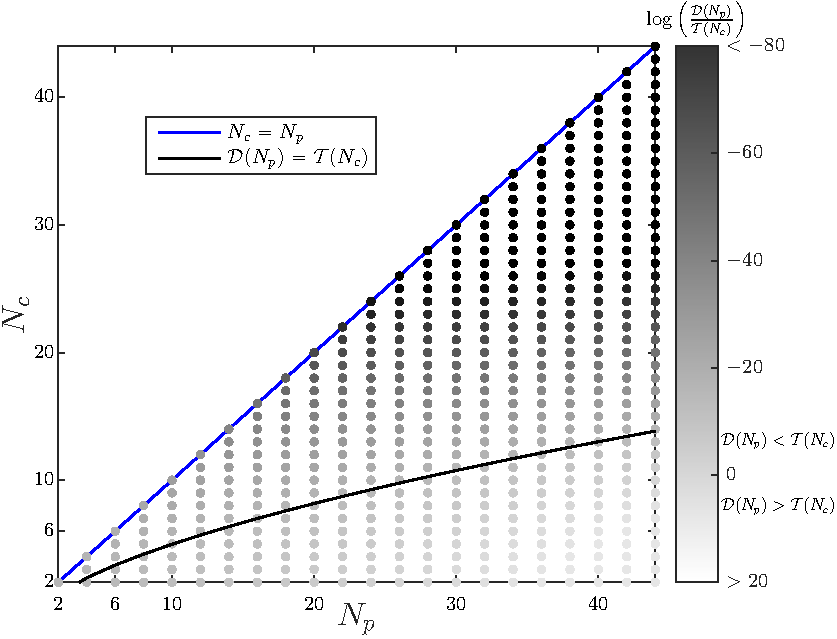
\includegraphics[width=0.6\columnwidth]{../ch2/figures/power2comparison}
\caption[Comparison between a \mypm{} approach and adjacency matrix approach.]{Comparison of number of graphs with \mypm{} approach and adjacency matrix approach.\label{fig:ch2:power2comparison}}
\end{figure}

A \mypm{} approach can be seen as an alternative to permuting all possible adjacency matrices assuming the architecture design problem is based on $(C,R,P)$ with NSC \ref{ch2:s6}. The question then becomes does every port being filled as in a \mypm{} approach result in all architectures defined by a certain architecture design problem?
Consider that we can always include 1-port components that represent empty connections, i.e.,~this component type implies that the vertex and edge can be removed from the graph without loss. We can control what components are allowed to have empty connections with \ref{ch2:s5}. Certain NSC sets such as \{\ref{ch2:s1}, \ref{ch2:s3} \ref{ch2:s4}, \ref{ch2:s7}\} would also require every port to be filled.

\subsection{Colored Graph Isomorphisms}

If we have a list of useful graphs, how many of them are truly different? Determining if two graphs are \textit{different} is known as the graph isomorphism problem. We define uniqueness among a set of architecture graphs to mean that no two candidate architectures are isomorphic.

\begin{definition}[Isomorphism] \label{def:ch2:iso}
Let $G = (V,E)$ and $G' = (V',E')$. We call $G$ and $G'$ isomorphic, and write $G \simeq G'$, if there exists a bijection $f: V\to V'$ with $(v_i,v_j) \in E \Leftrightarrow (f(v_i), f(v_j)) \in E'$ for all $v_i,v_j \in V$. The map $f$ is called an isomorphism \cite{Diestel2000a}.
\end{definition}

\begin{definition}[Colored Graph Isomorphism] \label{def:ch2:ciso}
The colored graph isomorphism problem is to decide the existence of a color preserving isomorphism between a pair of colored graphs $G = (V, E, L)$ and $G' = (V',E',L')$, i.e., a mapping $f: V \to V'$ satisfying the following conditions: \\
1. $f$ is an isomorphism by Definition~\ref{def:ch2:iso}. \\
2. $\mathrm{color}(v) = \mathrm{color}(f(v))$ for all $v \in V$.
\end{definition}

We can better understand how the colored graph isomorphism problem affects the architecture design problem by looking at two different isomorphisms: 
\begin{enumerate}[label=$\bullet$, widest=$\bullet$, nosep]

\item \textit{Port-type isomorphism} occurs when a component has ports that are indistinguishable in a modeling sense and can occur when using a ports representation. We have already termed such components as simple components. For example, consider a 2-port component that physically represents a mechanical translational spring. The two ports can be permuted and the resulting physical model will be equivalent. This demonstrated in Fig.~\ref{fig:ch2:piso} with the simple component type $\xcolor{G}$. $G^{CC}$ for the same graphs would be identical since the information about specific ports is lost. We leverage this fact to perform an initial port-type isomorphism filter to remove \mypm{}s that certainly have a port-type isomorphism. For a given simple $n$-port component, there are $n!$ ways to arrange the ports such that a port-type isomorphism occurs.

\begin{figure}
\centering
\begin{subfigure}[b]{2.5in}
\centering
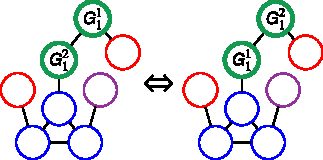
\includegraphics[width=\columnwidth]{../ch2/figures/pisopdf}
\caption{Port-type.\label{fig:ch2:piso}}
\end{subfigure}
\hspace{0.25in}
\begin{subfigure}[b]{2.5in}
\centering
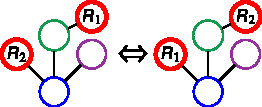
\includegraphics[width=\columnwidth]{../ch2/figures/cisopdf}
\caption{Component-type.\label{fig:ch2:ciso}}
\end{subfigure}
\caption{Two different type of isomorphisms.}
\end{figure}

\item \textit{Component-type isomorphism} occurs when switching a pair of component type  replicates preserves the graph. This type of isomorphism is present due to the arbitrary subscript numbers assigned to each vertex and is demonstrated in Fig.~\ref{fig:ch2:ciso}. The 1-port component type $\xcolor{R}$ is permuted but since $\xcolor{R}_1$ and $\xcolor{R}_2$ are the same component type, the graph remains the same (in the sense of Definition~\ref{def:ch2:ciso}). For $n$ replicates of a component type, there are $n!$ ways to arrange the components such that a component-type isomorphism occurs.

\end{enumerate}
We now define the final graph structure space $\mathcal{G}_3 \subseteq \mathcal{G}_2$ representing all unique useful graphs. Assuming no NSCs except those naturally satisfied by a \mypm{} approach, we can discern a very rough lower bound on the size of this set with:
\begin{align}\label{eq:ch2:lowerbnd}
\mathcal{D}(N_P) \times \prod_{i=1}^{n_C} \frac{1}{R_i! \times (P_i!)^{R_i}} \leq \abs*{\mathcal{G}_3} \leq \mathcal{D}(N_P)
\end{align}

\noindent where this formula assumes all port-type and component-type isomorphisms that could occur, do occur in the set of \mypm{}s. Consider $(C,R,P) = (\xcolor{A},6,1)$, then Eqn.~(\ref{eq:ch2:lowerbnd}) provides a lower bound of 0.02 graphs, but we know there is exactly 1 unique graph.

Although the graph isomorphism problem is NP (nondeterministic polynomial time), there are many efficient practical algorithms \cite{McKay2014a}. Study of the graph isomorphism problem is an ongoing field and recent breakthroughs could lead to improved algorithms \cite{Babai2016a}. In this work, we utilize the python package igraph using the \textsc{isomorphic\_vf2} function \cite{igraph} based on the VF2 algorithm \cite{Cordella2001a} to solve the colored isomorphism problem.

Many architecture design studies ignore the isomorphism problem but presence of isomorphic graphs leads to the evaluation of non-unique options \cite{Schmidt2000a}. For certain problem sizes, the complexity of checking for isomorphisms may be much greater than generating and evaluating new, potentially non-unique graphs. But to understand the effect of problem definition, NSCs, and candidate graph generation algorithms on $\mathcal{G}_3$ requires the isomorphism checks, and can lead to insights into new algorithms that naturally avoid the isomorphism problem \cite{Konigseder2016a}. Other graph generation algorithms have been developed that avoid isomorphic graphs \cite{Read1978a, Faulon2003b}. Furthermore, for appropriately sized problems, the isomorphism check is computationally viable.

% \IncMargin{1em}
\RestyleAlgo{algoruled}

\begin{vAlgorithm}[t]{\columnwidth}{0em}

\LinesNumbered
\SetSideCommentRight 
\DontPrintSemicolon
% \SetNoFillComment

% \SetTitleSty{\textsf}{small}
% \renewcommand{\algorithmcfname}{\small\textbf{\textsf{\MakeUppercase{Algorithm}}}}%

% \SetKwData{Left}{left}\SetKwData{This}{this}\SetKwData{Up}{up}
\SetKwFunction{cumprod}{cumprod}
\SetKwFunction{length}{length}
\SetKwFunction{zeros}{zeros}
\SetKwFunction{ceil}{ceil}
\SetKwFunction{mod}{mod}
\SetKwFunction{mymin}{min}
\SetKwFunction{detectiso}{isomorphic\_vf2}

\SetKwInOut{Input}{Input}
\SetKwInOut{Output}{Output}

\caption{Determination of the unique colored graphs given a set of colored graphs. \label{alg:ch2:cip}}

\Input{$\xvar{Graphs}$ -- set of colored graphs \\
$\xvar{Nbin}$ -- number of bins (for parallel processing)}
\Output{$\xvar{UniqueGraphs}$ -- set of unique colored graphs}
\BlankLine
            
$\xvar{ind}$ $\leftarrow$ $1$ \tcc*{initialize index for total unique graphs}

$\xvar{bin}(1).\xvar{Graphs}(1)$ $\leftarrow$ $\xvar{Graphs}(1)$  \tcc*{first graph is always unique}

	\For(\tcc*[f]{check remaining graphs}){$\xvar{i}\leftarrow$ $2$ \KwTo $\length(\xvar{Graphs})$ }{
	
		$\xvar{G1}$ $\leftarrow$ $\xvar{Graphs}(\xvar{i})$ \tcc*{current graph to check}
		
		\For(\textbf{in parallel} \tcc*[f]{check against each nonempty bin}){$\xvar{j}\leftarrow$ $1$ \KwTo $\mymin(\xvar{Nbin},\xvar{ind})$ }{
		
			$\xvar{k}$ $\leftarrow$ $\length(\xvar{bin(j).Graphs})$ \tcc*{unique graphs in bin}
         
        	$\xvar{IsoFlag}$ $\leftarrow$ $0$ \tcc*{initialize flag, 0 is not isomorphic}
        
        \tcc*[f]{while graphs remain and isomorphism not found}
        
        	\While(){$(\xvar{k} > 0)$ and $(\xvar{IsoFlag} = 0)$ }{
        	
        	$\xvar{G2}$ $\leftarrow$ $\xvar{bin}(\xvar{j}).\xvar{Graphs}(\xvar{k})$ \tcc*{a unique graph}
        
        	\If{\text{$\xvar{G1}$ and $\xvar{G2}$ pass preliminary isomorphism checks}}{
        	
        	$\xvar{IsoFlag}$ $\leftarrow$ $\detectiso(\xvar{G1},\xvar{G2})$ \tcc*{return 1 if G1 and G2 are isomorphic}
        	
        	}
        	        	
        	$\xvar{k}$ $\leftarrow$ $\xvar{k} - 1$ \tcc*{decrease index since G2 checked}
        
        	} % end while loop
        	
			$\xvar{results}(\xvar{j})$ $\leftarrow$ $\xvar{IsoFlag}$ \tcc*{assign result for bin c}
		
		} % end for c
		
		\If(\tcc*[f]{if no isomorphisms}){\text{all elements of  \xvar{results} are $0$} }{
		
        $\xvar{J}$ $\leftarrow$  $\mod(\xvar{ind}, \xvar{Nbin}) + 1$ \tcc*{index for next smallest bin}
        
        $\xvar{bin}(\xvar{J}).\xvar{Graphs}(\xvar{end}+1)$ $\leftarrow$ $\xvar{G1}$  \tcc*{assign to a bin}
        
        $\xvar{ind}$ $\leftarrow$ $\xvar{ind + 1}$ \tcc*{total unique graphs}
        
		
		} % end if statement
		
		
	} % end for i
	
	$\xvar{UniqueGraphs}$ $\leftarrow$  \text{combine graphs in $\xvar{bin}$ into a single set of graphs}

\end{vAlgorithm}

Algorithm~\ref{alg:ch2:cip} was developed to determine $\mathcal{G}_3$ given $\mathcal{G}_2$. This algorithm checks a candidate graph against bins of already found unique graphs and stops checking if an isomorphism is found, making it parallelizable to a degree and removes unnecessary checks. There are a number of quick preliminary checks that can be done between two graphs, as necessary conditions for them to be isomorphic include having the same number of vertices, edges, and color label distributions.

%------------------
\section{Tree Search Algorithm\label{sec:ch2:treesearch}}

With a better understanding of the colored graph isomorphism problem in the context of architecture design, a tree search algorithm was developed to more efficiently enumerate a graph structure space that contains $\mathcal{G}_3$. This algorithm is based on the idea that for simple components, the port ordering does not matter so we are free to always choose the first port of a component when making edges.
 
Algorithm~\ref{alg:ch2:simpletree} starts with a vector for length $N_C$ where the entries are the number of ports for every component in $G^{CC}$. For example, if $P = [1\ 2]$ and $R=[2\ 3]$, then this vector would be $\xvar{V} = [1\ 1\ 2\ 2\ 2]$ and $\xvar{cVf} = [2\ 3\ 5\ 7\ 9]$. Recursion is then applied to enumerate all possible edge combinations where each recursive step adds an edge. The end result is a set of missorted \mypm{}s, i.e.,~the sequential pairs that define the edges need to be sorted such that they fit the definition of a \mypm{} in Sec.~\ref{sec:ch2:inter} (but no \mypm{} will occur twice and the property of naturally satisfying \ref{ch2:s2} and \ref{ch2:s6} is maintained). The end result is an algorithm that does not produce many \mypm{} graphs that would certainly have a port-type isomorphism. A visualization of the tree-like behavior is in Fig.~\ref{fig:ch2:tree1simple} where each leaf in the tree is a new call of the algorithm and the branches are the loops through the possible remaining edges. Not all leaves have the same number of branches since components become completely connected at different times. Two paths are shown in the figure for a particular architecture design problem, each resulting in a different \mypm{}. Note that the thicker black lines indicate the chosen edge and the gray lines are the other potential edges for the particular leaf instance.

\begin{figure}
\centering
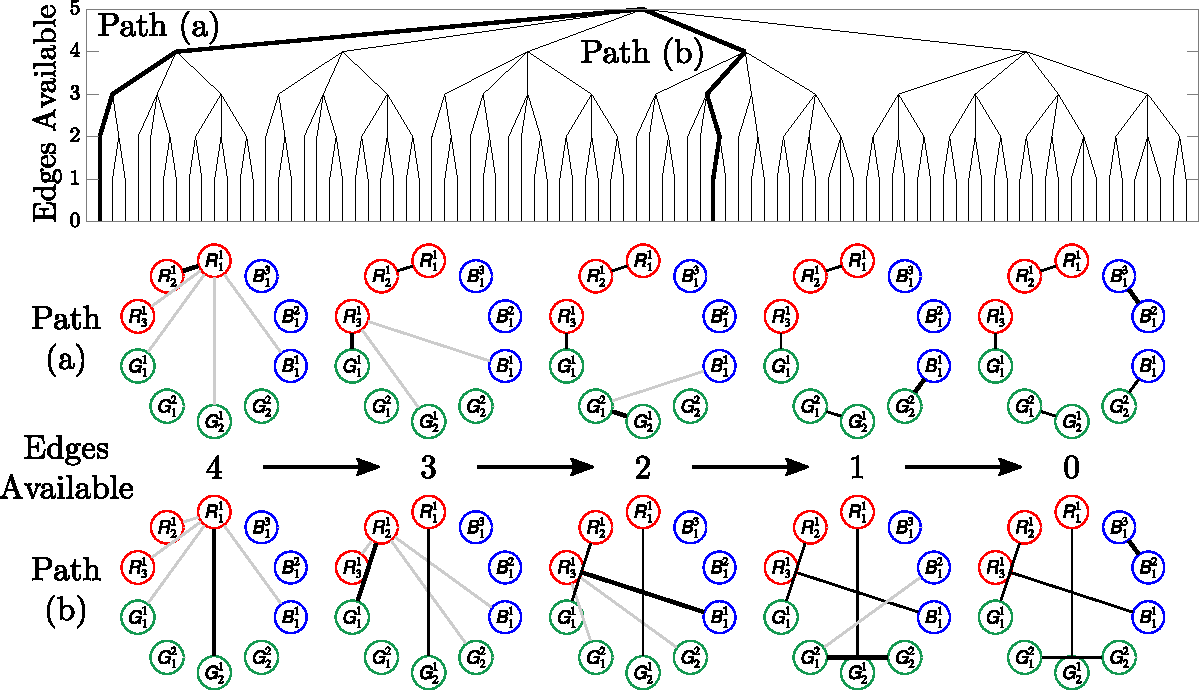
\includegraphics[width=\columnwidth]{../ch2/figures/tree1simple_optimized}
\caption[Tree structure for \nameref{sec:ch2:example1} using the basic tree search algorithm]{Tree structure for \nameref{sec:ch2:example1} using the basic tree search algorithm in Alg.~\ref{alg:ch2:simpletree}.\label{fig:ch2:tree1simple}}
\end{figure}

This approach is similar to a number of reported graph enumeration algorithms \cite{Carhart1975a, Colbourn1979a, Snavely1993a, Faulon2003b}.
The tree algorithm shares some similarities with deletion orderly algorithms \cite{Colbourn1979a}.
Snavely and Papalambros developed a tree algorithm that only deals with structured components, which limits the design space by the number of components rather than the $(C,R,P)$ notation in this work \cite{Snavely1993a}. 
Faulon et al. enumerate molecules of a specific signature height with a recursive algorithm, but do not allow for components to be removed. Thus, they do not cover the same architecture design space \cite{Faulon2003b}. 
Neither of these works make the connection between \mypm{} theory and architecture enumeration which provides a number of insights and practical functions. 

We can further improve on this algorithm by adding a single line between lines~\ref{ch2:line3} and \ref{ch2:line4} that will result in graphs that always satisfy \ref{ch2:s5} (feasible edge constraints). First, expand $A_R$ such that its size is the same as $G^{CC}$ where 0 entries still indicate infeasible edge constraints. The additional line would then be: $\xvar{Vallow}$ $\leftarrow$  $\xvar{A}(\xvar{iL},:) \circ \xvar{V}$. By finding the nonzero entries of $\xvar{Vallow}$ instead of $\xvar{V}$, we limit the for-loop to edges that are feasible. This has the intentional effect that certain branches of the tree will terminate before a feasible \mypm{} is found. Therefore when \ref{ch2:s5} is present, we will utilize this `improved' tree search algorithm to more efficiently enumerate $\mathcal{G}_3$.
Additional enhancements to the tree search algorithm are discussed in Appendix~\ref{app:A} as well as alternative tree traversal strategies.

% \IncMargin{1em}
\RestyleAlgo{algoruled}

\begin{vAlgorithm}[t]{\columnwidth}{0em}

\LinesNumbered
\SetSideCommentRight 
\DontPrintSemicolon
% \SetNoFillComment

% \SetTitleSty{\textsf}{small}
% \renewcommand{\algorithmcfname}{\small\textbf{\textsf{\MakeUppercase{Algorithm}}}}%

% \SetKwData{Left}{left}\SetKwData{This}{this}\SetKwData{Up}{up}
\SetKwFunction{cumprod}{cumprod}
\SetKwFunction{length}{length}
\SetKwFunction{zeros}{zeros}
\SetKwFunction{ceil}{ceil}
\SetKwFunction{mod}{mod}
\SetKwFunction{mymin}{min}
\SetKwFunction{find}{find}
\SetKwFunction{detectiso}{isomorphic\_vf2}

\SetKwInOut{Input}{Input}
\SetKwInOut{Output}{Output}

\caption{Basic tree search algorithm. \label{alg:ch2:simpletree}}

\Input{$\xvar{V}$ -- vector of remaining ports for each component replicate \\
$\xvar{E}$ -- vector of edges in sequential pairs, initially empty \\
$\xvar{cVf}$ -- cumulative sum of the original $\xvar{V}$ plus 1 \\
$\xvar{SavedGraphs}$ -- set of graphs, initially empty \\
}
\Output{$\xvar{SavedGraphs}$ -- set of graphs \\
}
\BlankLine
            
    $\xvar{iL}$ $\leftarrow$  $\find(\xvar{V},\xvar{first})$ \tcc*{find first nonzero entry}
    
    $\xvar{L}$ $\leftarrow$  $\xvar{cVf}(\xvar{iL})-\xvar{V}(\xvar{iL})$ \tcc*{left port}
    
    $\xvar{V}\big(\xvar{I}(1)\big)$ $\leftarrow$ $\xvar{V}(\xvar{iL}) - 1$ \tcc*{remove port \label{ch2:line3}}
    
% \SetSideCommentLeft 
  %   \tcc*{$\xvar{V}$ $\leftarrow$  $\xvar{A}(\xvar{I}(1),:) \circ \xvar{V}$, naturally enforce \ref{ch2:s5} by using a potential adjacency matrix $\xvar{A}$}
% \SetSideCommentRight   
            
    $\xvar{I}$ $\leftarrow$  $\find(\xvar{V})$ \tcc*{find nonzero entries \label{ch2:line4}}  
    
	\For(\tcc*[f]{loop through all nonzero entries}){$\xvar{iR}\leftarrow$ $\xvar{I}$ \label{alg:ch2:cip:5} }{
	
        $\xvar{R}$ $\leftarrow$ $\xvar{cVf}(\xvar{iR})-\xvar{V}(\xvar{iR})$ \tcc*{right port}

        $\xvar{E2}$ $\leftarrow$ $[\xvar{E},\xvar{L},\xvar{R}]$ \tcc*{combine left, right ports for an edge }

		$\xvar{V2}$ $\leftarrow$ $\xvar{V}$ \tcc*{local remaining ports vector}
       
		% $\xvar{Eo}$ $\leftarrow$ $\xvar{E}$
               
        $\xvar{V2}(\xvar{iR})$ $\leftarrow$ $\xvar{V2}(\xvar{iR})-1$ \tcc*{remove port (local copy)}
	
		\uIf(\tcc*[f]{recursive call if any remaining vertices}){any element of $\xvar{V2}$ is nonzero}{
		
            $\xvar{SavedGraphs}$ $\leftarrow$ Algorithm~\ref{alg:ch2:simpletree} with $\xvar{V2},\xvar{E2},\xvar{cVf},\xvar{SavedGraphs}$
            
        }
        	
        \Else{
        	
            % $\xvar{id}$  $\leftarrow$ $\xvar{id}+1$ \tcc*{increment index of total graphs}
            
            $\xvar{SavedGraphs}\{\xvar{end} + 1\}$  $\leftarrow$ $\xvar{E2}$ \tcc*{save missorted perfect matching }
        	
        }
	
	} % end for i

\end{vAlgorithm}

%------------------
\section{Enumeration Case Studies\label{sec:ch2:simple}}

In this section, a number of case studies are provided to demonstrate the theoretical aspects of the previous sections\footnote{Ref.~\cite{github-pm-architectures-project} contains \xprog{Matlab} codes that replicate the results from these enumeration case studies and can generate graphs for $(C,R,P)$ architecture design problems.}.

\subsection{Case Study 1\label{sec:ch2:example1}}

\begin{figure}
\centering

\tikzsetnextfilename{cpexamples}

\begin{subfigure}[b]{1\columnwidth}
\centering
% \cfbox{box-gray}{
\resizebox{!}{12mm}{
\begin{tikzpicture}[
mynode/.style={draw, circle, very thick, inner sep=1pt, scale=1.3},
myline/.style={draw, very thick},
]

\node[mynode,draw=red] (1) at (-2,-0) {$\xcolor{R}_1^1$};
\node[mynode,draw=red] (2) at (-1,-1) {$\xcolor{R}_2^1$};
\node[mynode,draw=red] (3) at (0,0) {$\xcolor{R}_3^1$};
\node[mynode,draw=ForestGreen] (4) at (1,-1) {$\xcolor{G}_1^1$};
\node[mynode,draw=ForestGreen] (5) at (2,0) {$\xcolor{G}_1^2$};
\node[mynode,draw=ForestGreen] (6) at (3,-1) {$\xcolor{G}_2^1$};
\node[mynode,draw=ForestGreen] (7) at (4,0) {$\xcolor{G}_2^2$};
\node[mynode,draw=blue] (8) at (5,-1) {$\xcolor{B}_1^1$};
\node[mynode,draw=blue] (9) at (6,0) {$\xcolor{B}_1^2$};
\node[mynode,draw=blue] (10) at (7,-1) {$\xcolor{B}_1^3$};

\draw [myline] (4) -- (5);
\draw [myline] (6) -- (7);
\draw [myline] (8) -- (9);
\draw [myline] (8) -- (10);
\draw [myline] (9) -- (10);

\end{tikzpicture}
}
% } 
\caption{\nameref{sec:ch2:example1}. \label{fig:ch2:cpexamples:1}}
\end{subfigure}

\begin{subfigure}[b]{1\columnwidth}
\centering
% \cfbox{box-gray}{
\resizebox{!}{12mm}{
\begin{tikzpicture}[
mynode/.style={draw, circle, very thick, inner sep=1pt, scale=1.3},
myline/.style={draw, very thick},
]

\node[mynode,draw=Purple] (1) at (-2,0) {$\xcolor{P}_1^1$};
\node[mynode,draw=red] (2) at (-1,-1) {$\xcolor{R}_1^1$};
\node[mynode,draw=red] (3) at (0,0) {$\xcolor{R}_2^1$};
\node[mynode,draw=ForestGreen] (4) at (1,-1) {$\xcolor{G}_1^1$};
\node[mynode,draw=ForestGreen] (5) at (2,0) {$\xcolor{G}_1^2$};
\node[mynode,draw=ForestGreen] (6) at (3,-1) {$\xcolor{G}_2^1$};
\node[mynode,draw=ForestGreen] (7) at (4,0) {$\xcolor{G}_2^2$};
\node[mynode,draw=blue] (8) at (5,-1) {$\xcolor{B}_1^1$};
\node[mynode,draw=blue] (9) at (6,0) {$\xcolor{B}_1^2$};
\node[mynode,draw=blue] (10) at (7,-1) {$\xcolor{B}_1^3$};
\node[mynode,draw=YellowOrange] (11) at (8,0) {$\xcolor{O}_1^1$};
\node[mynode,draw=YellowOrange] (12) at (9,-1) {$\xcolor{O}_1^2$};
\node[mynode,draw=YellowOrange] (13) at (10,0) {$\xcolor{O}_1^3$};
\node[mynode,draw=YellowOrange] (14) at (11,-1) {$\xcolor{O}_1^4$};

\draw [myline] (4) -- (5);
\draw [myline] (6) -- (7);
\draw [myline] (8) -- (9);
\draw [myline] (8) -- (10);
\draw [myline] (9) -- (10);
\draw [myline] (11) -- (12);
\draw [myline] (11) -- (13);
\draw [myline] (12) -- (13);
\draw [myline] (11) -- (14);
\draw [myline] (12) -- (14);
\draw [myline] (13) -- (14);

\end{tikzpicture}
}
% }
\caption{\nameref{sec:ch2:example2}. \label{fig:ch2:cpexamples:2}}
\end{subfigure}

\caption{$G^{P}$ graphs for two examples. \label{fig:cpexamples}}

\end{figure}



\begin{figure}
\centering

\begin{subfigure}[b]{0.25\columnwidth}
\centering
\cfbox{box-gray}{
\resizebox{!}{\textwidth}{
\tikzsetnextfilename{inter11}
\begin{tikzpicture}[
mynode/.style={draw, circle, very thick, inner sep=1pt, scale=1.3},
myline/.style={draw, very thick},
]
\pgfmathsetmacro{\n}{10};
\pgfmathsetmacro{\r}{2.5};

\node[mynode,draw=red] (1) at (0*360/\n + 90: \r cm) {$\xcolor{R}_1^1$};
\node[mynode,draw=red] (2) at (1*360/\n + 90: \r cm) {$\xcolor{R}_2^1$};
\node[mynode,draw=red] (3) at  (2*360/\n + 90: \r cm) {$\xcolor{R}_3^1$};
\node[mynode,draw=ForestGreen] (4) at  (3*360/\n + 90: \r cm) {$\xcolor{G}_1^1$};
\node[mynode,draw=ForestGreen] (5) at  (4*360/\n + 90: \r cm) {$\xcolor{G}_1^2$};
\node[mynode,draw=ForestGreen] (6) at  (5*360/\n + 90: \r cm) {$\xcolor{G}_2^1$};
\node[mynode,draw=ForestGreen] (7) at  (6*360/\n + 90: \r cm) {$\xcolor{G}_2^2$};
\node[mynode,draw=blue] (8) at  (7*360/\n + 90: \r cm) {$\xcolor{B}_1^1$};
\node[mynode,draw=blue] (9) at  (8*360/\n + 90: \r cm) {$\xcolor{B}_1^2$};
\node[mynode,draw=blue] (10) at  (9*360/\n + 90: \r cm) {$\xcolor{B}_1^3$};

\foreach \i in {1,...,\n}{
	\foreach \j in {\i,...,\n}{
    	\draw [myline,light-gray] (\i) -- (\j);
} }

\end{tikzpicture}
}
}
\caption{$K_{10}$.\label{fig:ch2:inter1_1}}
\end{subfigure}
%
% \hspace{0.02\textwidth}
%
\begin{subfigure}[b]{0.25\columnwidth}
\centering
\cfbox{box-gray}{
\resizebox{!}{\textwidth}{
\tikzsetnextfilename{inter12}
\begin{tikzpicture}[
mynode/.style={draw, circle, very thick, inner sep=1pt, scale=1.3},
myline/.style={draw, very thick},
]
\pgfmathsetmacro{\n}{10};
\pgfmathsetmacro{\r}{2.5};

\node[mynode,draw=red] (1) at (0*360/\n + 90: \r cm) {$\xcolor{R}_1^1$};
\node[mynode,draw=red] (2) at (1*360/\n + 90: \r cm) {$\xcolor{R}_2^1$};
\node[mynode,draw=red] (3) at  (2*360/\n + 90: \r cm) {$\xcolor{R}_3^1$};
\node[mynode,draw=ForestGreen] (4) at  (3*360/\n + 90: \r cm) {$\xcolor{G}_1^1$};
\node[mynode,draw=ForestGreen] (5) at  (4*360/\n + 90: \r cm) {$\xcolor{G}_1^2$};
\node[mynode,draw=ForestGreen] (6) at  (5*360/\n + 90: \r cm) {$\xcolor{G}_2^1$};
\node[mynode,draw=ForestGreen] (7) at  (6*360/\n + 90: \r cm) {$\xcolor{G}_2^2$};
\node[mynode,draw=blue] (8) at  (7*360/\n + 90: \r cm) {$\xcolor{B}_1^1$};
\node[mynode,draw=blue] (9) at  (8*360/\n + 90: \r cm) {$\xcolor{B}_1^2$};
\node[mynode,draw=blue] (10) at  (9*360/\n + 90: \r cm) {$\xcolor{B}_1^3$};

\draw [myline] (10) -- (1);
\draw [myline] (9) -- (2);
\draw [myline] (8) -- (3);
\draw [myline] (7) -- (4);
\draw [myline] (6) -- (5);

\end{tikzpicture}
}
}
\caption{\mypm{}~1.\label{fig:ch2:inter1_2}}
\end{subfigure}
%
% \hspace{0.02\textwidth}
%
\begin{subfigure}[b]{0.25\columnwidth}
\centering
\cfbox{box-gray}{
\resizebox{!}{\textwidth}{
\tikzsetnextfilename{inter13}
\begin{tikzpicture}[
mynode/.style={draw, circle, very thick, inner sep=1pt, scale=1.3},
myline/.style={draw, very thick},
]
\pgfmathsetmacro{\n}{10};
\pgfmathsetmacro{\r}{2.5};

\node[mynode,draw=red] (1) at (0*360/\n + 90: \r cm) {$\xcolor{R}_1^1$};
\node[mynode,draw=red] (2) at (1*360/\n + 90: \r cm) {$\xcolor{R}_2^1$};
\node[mynode,draw=red] (3) at  (2*360/\n + 90: \r cm) {$\xcolor{R}_3^1$};
\node[mynode,draw=ForestGreen] (4) at  (3*360/\n + 90: \r cm) {$\xcolor{G}_1^1$};
\node[mynode,draw=ForestGreen] (5) at  (4*360/\n + 90: \r cm) {$\xcolor{G}_1^2$};
\node[mynode,draw=ForestGreen] (6) at  (5*360/\n + 90: \r cm) {$\xcolor{G}_2^1$};
\node[mynode,draw=ForestGreen] (7) at  (6*360/\n + 90: \r cm) {$\xcolor{G}_2^2$};
\node[mynode,draw=blue] (8) at  (7*360/\n + 90: \r cm) {$\xcolor{B}_1^1$};
\node[mynode,draw=blue] (9) at  (8*360/\n + 90: \r cm) {$\xcolor{B}_1^2$};
\node[mynode,draw=blue] (10) at  (9*360/\n + 90: \r cm) {$\xcolor{B}_1^3$};

\draw [myline] (10) -- (5);
\draw [myline] (9) -- (3);
\draw [myline] (8) -- (6);
\draw [myline] (7) -- (4);
\draw [myline] (2) -- (1);

\end{tikzpicture}
}
}
\caption{\mypm{}~462.\label{fig:ch2:inter1_3}}
\end{subfigure}


\caption{Select interconnectivity graphs for \nameref{sec:ch2:example1}.\label{fig:ch2:inter1}}

\end{figure}

% \draw [] (10) -- (9);
% \draw [] (8) -- (2);
% \draw [] (7) -- (4);
% \draw [] (6) -- (5);
% \draw [] (3) -- (1);
% \caption{ 864 of 945 }

\begin{figure}
\centering

\begin{subfigure}[b]{0.25\columnwidth}
\centering
\cfbox{box-gray}{
\resizebox{!}{\textwidth}{
\tikzsetnextfilename{model1_1}
\begin{tikzpicture}[
mynode/.style={draw, circle, very thick, inner sep=1pt, scale=1.3},
myline/.style={draw, very thick},
]
\pgfmathsetmacro{\n}{10};
\pgfmathsetmacro{\r}{2.5};

\node[mynode,draw=red] (1) at (0*360/\n + 90: \r cm) {$\xcolor{R}_1^1$};
\node[mynode,draw=red] (2) at (1*360/\n + 90: \r cm) {$\xcolor{R}_2^1$};
\node[mynode,draw=red] (3) at  (2*360/\n + 90: \r cm) {$\xcolor{R}_3^1$};
\node[mynode,draw=ForestGreen] (4) at  (3*360/\n + 90: \r cm) {$\xcolor{G}_1^1$};
\node[mynode,draw=ForestGreen] (5) at  (4*360/\n + 90: \r cm) {$\xcolor{G}_1^2$};
\node[mynode,draw=ForestGreen] (6) at  (5*360/\n + 90: \r cm) {$\xcolor{G}_2^1$};
\node[mynode,draw=ForestGreen] (7) at  (6*360/\n + 90: \r cm) {$\xcolor{G}_2^2$};
\node[mynode,draw=blue] (8) at  (7*360/\n + 90: \r cm) {$\xcolor{B}_1^1$};
\node[mynode,draw=blue] (9) at  (8*360/\n + 90: \r cm) {$\xcolor{B}_1^2$};
\node[mynode,draw=blue] (10) at  (9*360/\n + 90: \r cm) {$\xcolor{B}_1^3$};


\draw [myline] (10) -- (1);
\draw [myline] (9) -- (2);
\draw [myline] (8) -- (3);
\draw [myline] (7) -- (4);
\draw [myline] (6) -- (5);

\draw [myline] (4) -- (5);
\draw [myline] (6) -- (7);
\draw [myline] (8) -- (9);
\draw [myline] (8) -- (10);
\draw [myline] (9) -- (10);

\end{tikzpicture}
}
}
\caption{$G^{CP}$  for  \mypm{}~1.\label{fig:ch2:model1_1}}
\end{subfigure}
%
% \hspace{0.02\textwidth}
%
\begin{subfigure}[b]{0.25\columnwidth}
\centering
\cfbox{box-gray}{
\resizebox{!}{\textwidth}{
\tikzsetnextfilename{model1_2}
\begin{tikzpicture}[
mynode/.style={draw, circle, very thick, inner sep=1pt, scale=1.3},
myline/.style={draw, very thick},
]
\pgfmathsetmacro{\n}{6};
\pgfmathsetmacro{\r}{1.5};

\node[mynode,draw=red] (1) at (0*360/\n + 90: \r cm) {$\xcolor{R}$};
\node[mynode,draw=red] (2) at (1*360/\n + 90: \r cm) {$\xcolor{R}$};
\node[mynode,draw=red] (3) at  (2*360/\n + 90: \r cm) {$\xcolor{R}$};
\node[mynode,draw=ForestGreen] (4) at  (3*360/\n + 90: \r cm) {$\xcolor{G}$};
\node[mynode,draw=ForestGreen] (5) at  (4*360/\n + 90: \r cm) {$\xcolor{G}$};
\node[mynode,draw=blue, circle] (6) at  (5*360/\n + 90: \r cm) {$\xcolor{B}$};

\draw [myline] (1) -- (6);
\draw [myline] (2) -- (6);
\draw [myline] (3) -- (6);
\draw [myline] (4) -- (5);

\end{tikzpicture}
}
}
\caption{$G^{CC}$  for  \mypm{}~1.\label{fig:ch2:model1_2}}
\end{subfigure}
%
% \hspace{0.02\textwidth}
%
%\begin{subfigure}[b]{0.32\columnwidth}
%\centering
%\cfbox{box-gray}{
%\resizebox{!}{\textwidth}{
%\tikzsetnextfilename{model1_3}
%\begin{tikzpicture}[
%mynode/.style={draw, circle, very thick, inner sep=1pt, scale=1.3},
%myline/.style={draw, very thick},
%]
%\pgfmathsetmacro{\n}{10};
%\pgfmathsetmacro{\r}{2.5};
%
%\node[mynode,draw=red] (1) at (0*360/\n + 90: \r cm) {$\xcolor{R}_1^1$};
%\node[mynode,draw=red] (2) at (1*360/\n + 90: \r cm) {$\xcolor{R}_2^1$};
%\node[mynode,draw=red] (3) at  (2*360/\n + 90: \r cm) {$\xcolor{R}_3^1$};
%\node[mynode,draw=ForestGreen] (4) at  (3*360/\n + 90: \r cm) {$\xcolor{G}_1^1$};
%\node[mynode,draw=ForestGreen] (5) at  (4*360/\n + 90: \r cm) {$\xcolor{G}_1^2$};
%\node[mynode,draw=ForestGreen] (6) at  (5*360/\n + 90: \r cm) {$\xcolor{G}_2^1$};
%\node[mynode,draw=ForestGreen] (7) at  (6*360/\n + 90: \r cm) {$\xcolor{G}_2^2$};
%\node[mynode,draw=blue] (8) at  (7*360/\n + 90: \r cm) {$\xcolor{B}_1^1$};
%\node[mynode,draw=blue] (9) at  (8*360/\n + 90: \r cm) {$\xcolor{B}_1^2$};
%\node[mynode,draw=blue] (10) at  (9*360/\n + 90: \r cm) {$\xcolor{B}_1^3$};
%
%
%\draw [myline] (10) -- (5);
%\draw [myline] (9) -- (3);
%\draw [myline] (8) -- (6);
%\draw [myline] (7) -- (4);
%\draw [myline] (2) -- (1);
%
%\draw [myline] (4) -- (5);
%\draw [myline] (6) -- (7);
%\draw [myline] (8) -- (9);
%\draw [myline] (8) -- (10);
%\draw [myline] (9) -- (10);
%
%\end{tikzpicture}
%}
%}
%\caption{$G^{CP}$  for  \mypm{}~462.\label{fig:model1_3}}
%\end{subfigure}
%%
%\hspace{0.02\textwidth}
%%
\begin{subfigure}[b]{0.25\columnwidth}
\centering
\cfbox{box-gray}{
\resizebox{!}{\textwidth}{
\tikzsetnextfilename{model1_4}
\begin{tikzpicture}[
mynode/.style={draw, circle, very thick, inner sep=1pt, scale=1.3},
myline/.style={draw, very thick},
]
\pgfmathsetmacro{\n}{6};
\pgfmathsetmacro{\r}{1.5};

\node[mynode,draw=red] (1) at (0*360/\n + 90: \r cm) {$\xcolor{R}$};
\node[mynode,draw=red] (2) at (1*360/\n + 90: \r cm) {$\xcolor{R}$};
\node[mynode,draw=red] (3) at  (2*360/\n + 90: \r cm) {$\xcolor{R}$};
\node[mynode,draw=ForestGreen] (4) at  (3*360/\n + 90: \r cm) {$\xcolor{G}$};
\node[mynode,draw=ForestGreen] (5) at  (4*360/\n + 90: \r cm) {$\xcolor{G}$};
\node[mynode,draw=blue, circle] (6) at  (5*360/\n + 90: \r cm) {$\xcolor{B}$};

\draw [myline] (1) -- (2);
\draw [myline] (3) -- (6);
\draw [myline] (4) -- (6);
\draw [myline] (5) -- (6);
\draw [myline] (5) -- (4);

\end{tikzpicture}
}
}
\caption{$G^{CC}$ for \mypm{}~462.\label{fig:ch2:model1_4}}
\end{subfigure}

\caption{Select connected ports and connected component graphs for \nameref{sec:ch2:example1}.\label{fig:model1}}

\end{figure}

The base three-tuple is specified as:
\begin{align*}
{C} &= \left\lbrace \xcolor{R}, \xcolor{G}, \xcolor{B} \right\rbrace, \qquad {R} = [ 3, 2, 1 ], \qquad {P} = [ 1, 2, 3 ]
\end{align*}

\noindent This example has three different simple component types that have multiple ports and replicates and is visualized in Fig.~\ref{fig:ch2:cpexamples:1}. Then $G^{P}$ is:
\begin{align*}
{V}^{P} &= \left\lbrace  1, 2, 3, 4, 5, 6, 7, 8, 9, 10 \right\rbrace \\
{E}^{P} &= \left\lbrace  (4,5), (6,7), (8,9), (8,10), (9,10) \right\rbrace \\
{L}^{P} &= \left\lbrace \xcolor{R}_1^1, \xcolor{R}_2^1, \xcolor{R}_3^1, \xcolor{G}_1^1, \xcolor{G}_1^2, \xcolor{G}_2^1, \xcolor{G}_2^2, \xcolor{B}_1^1, \xcolor{B}_1^2, \xcolor{B}_1^3 \right\rbrace \\
N_P &= 10, \quad N_C = 6, \quad 3.28 \leq \abs*{\mathcal{G}_3} \leq 945
\end{align*}

\noindent In Fig.~\ref{fig:ch2:inter1} we see $G^{I}$ for two different \mypm{}s. Then in Fig.~\ref{fig:ch2:model1_1} we can see $G^{CP}$ for \mypm{}~1. This can then be mapped to the equivalent $G^{CC}$ shown in Fig.~\ref{fig:ch2:model1_2}. The basic tree search algorithm will have the same tree regardless of the NSCs and this tree is visualized in Fig.~\ref{fig:ch2:tree1simple}. Both graphs in Figs.~\ref{fig:ch2:model1_2} and \ref{fig:ch2:model1_4} will have a topologically equivalent graph appear in the set of graphs generated by this algorithm. Now two different sets of NSCs will be discussed.

\begin{enumerate}[nosep]

\item \label{ch2:example11} No additional NSCs. There are 32,768 adjacency matrices ($\mathcal{G}_0$);  945 \mypm{}s ($\mathcal{G}_1$); 86 candidate graphs with basic tree search algorithm; 77 remaining candidate graphs after initial port-type isomorphism filter; and 77 feasible graphs ($\mathcal{G}_2$). Finally, there are only 16 unique graphs ($\mathcal{G}_3$) consistent with Eqn.~(\ref{eq:ch2:lowerbnd}) and all shown in Fig.~\ref{fig:ch2:unique1}. 258 graph comparisons were needed and only 113 required a full isomorphism check.

\begin{figure*}

\definecolor{R}{rgb}{1,0,0} % red
\definecolor{G}{rgb}{0,0.6,0.36078431372} % forestgreen
\definecolor{B}{rgb}{0,0,1} % blue
\definecolor{O}{rgb}{0.99607843137,0.63529411764,0.22745098039} % orange
\definecolor{P}{rgb}{0.60784313725,0.27843137254,0.58823529411} % purple
\centering
% \newcommand{\uniquesize}{0.115\textwidth}
\newcommand{\uniquesize}{0.14\textwidth}
%
%
%
\begin{subfigure}[b]{\uniquesize}
\centering
\resizebox{!}{\textwidth}{
\begin{tikzpicture}[
mynode/.style={draw, circle, very thick, inner sep=1pt, scale=1.3},
myline/.style={draw, very thick},
]
\pgfmathsetmacro{\n}{6};
\pgfmathsetmacro{\r}{1.5};
\node[mynode,draw=R] (1) at (0*360/\n + 90: \r cm) {$\xcolor{R}$};
\node[mynode,draw=R] (2) at (1*360/\n + 90: \r cm) {$\xcolor{R}$};
\node[mynode,draw=R] (3) at (2*360/\n + 90: \r cm) {$\xcolor{R}$};
\node[mynode,draw=G] (4) at (3*360/\n + 90: \r cm) {$\xcolor{G}$};
\node[mynode,draw=G] (5) at (4*360/\n + 90: \r cm) {$\xcolor{G}$};
\node[mynode,draw=B] (6) at (5*360/\n + 90: \r cm) {$\xcolor{B}$};
\draw [myline] (6) -- (1);
\draw [myline] (6) -- (2);
\draw [myline] (6) -- (3);
\draw [myline] (5) -- (4);
\end{tikzpicture}
}
\caption{\mypm{}~227}
\end{subfigure}
%
%
%
\begin{subfigure}[b]{\uniquesize}
\centering
\resizebox{!}{\textwidth}{
\begin{tikzpicture}[
mynode/.style={draw, circle, very thick, inner sep=1pt, scale=1.3},
myline/.style={draw, very thick},
]
\pgfmathsetmacro{\n}{6};
\pgfmathsetmacro{\r}{1.5};
\node[mynode,draw=R] (1) at (0*360/\n + 90: \r cm) {$\xcolor{R}$};
\node[mynode,draw=R] (2) at (1*360/\n + 90: \r cm) {$\xcolor{R}$};
\node[mynode,draw=R] (3) at (2*360/\n + 90: \r cm) {$\xcolor{R}$};
\node[mynode,draw=G] (4) at (3*360/\n + 90: \r cm) {$\xcolor{G}$};
\node[mynode,draw=G] (5) at (4*360/\n + 90: \r cm) {$\xcolor{G}$};
\node[mynode,draw=B] (6) at (5*360/\n + 90: \r cm) {$\xcolor{B}$};
\draw [myline] (6) -- (1);
\draw [myline] (6) -- (2);
\draw [myline] (6) -- (3);
\end{tikzpicture}
}
\caption{\mypm{}~228}
\end{subfigure}
%
%
%
\begin{subfigure}[b]{\uniquesize}
\centering
\resizebox{!}{\textwidth}{
\begin{tikzpicture}[
mynode/.style={draw, circle, very thick, inner sep=1pt, scale=1.3},
myline/.style={draw, very thick},
]
\pgfmathsetmacro{\n}{6};
\pgfmathsetmacro{\r}{1.5};
\node[mynode,draw=R] (1) at (0*360/\n + 90: \r cm) {$\xcolor{R}$};
\node[mynode,draw=R] (2) at (1*360/\n + 90: \r cm) {$\xcolor{R}$};
\node[mynode,draw=R] (3) at (2*360/\n + 90: \r cm) {$\xcolor{R}$};
\node[mynode,draw=G] (4) at (3*360/\n + 90: \r cm) {$\xcolor{G}$};
\node[mynode,draw=G] (5) at (4*360/\n + 90: \r cm) {$\xcolor{G}$};
\node[mynode,draw=B] (6) at (5*360/\n + 90: \r cm) {$\xcolor{B}$};
\draw [myline] (6) -- (1);
\draw [myline] (6) -- (2);
\draw [myline] (5) -- (3);
\draw [myline] (5) -- (4);
\draw [myline] (6) -- (4);
\end{tikzpicture}
}
\caption{\mypm{}~332}
\end{subfigure}
%
%
%
\begin{subfigure}[b]{\uniquesize}
\centering
\resizebox{!}{\textwidth}{
\begin{tikzpicture}[
mynode/.style={draw, circle, very thick, inner sep=1pt, scale=1.3},
myline/.style={draw, very thick},
]
\pgfmathsetmacro{\n}{6};
\pgfmathsetmacro{\r}{1.5};
\node[mynode,draw=R] (1) at (0*360/\n + 90: \r cm) {$\xcolor{R}$};
\node[mynode,draw=R] (2) at (1*360/\n + 90: \r cm) {$\xcolor{R}$};
\node[mynode,draw=R] (3) at (2*360/\n + 90: \r cm) {$\xcolor{R}$};
\node[mynode,draw=G] (4) at (3*360/\n + 90: \r cm) {$\xcolor{G}$};
\node[mynode,draw=G] (5) at (4*360/\n + 90: \r cm) {$\xcolor{G}$};
\node[mynode,draw=B] (6) at (5*360/\n + 90: \r cm) {$\xcolor{B}$};
\draw [myline] (6) -- (1);
\draw [myline] (6) -- (2);
\draw [myline] (4) -- (3);
\draw [myline] (6) -- (4);
\end{tikzpicture}
}
\caption{\mypm{}~438}
\end{subfigure}
%
%
%
\begin{subfigure}[b]{\uniquesize}
\centering
\resizebox{!}{\textwidth}{
\begin{tikzpicture}[
mynode/.style={draw, circle, very thick, inner sep=1pt, scale=1.3},
myline/.style={draw, very thick},
]
\pgfmathsetmacro{\n}{6};
\pgfmathsetmacro{\r}{1.5};
\node[mynode,draw=R] (1) at (0*360/\n + 90: \r cm) {$\xcolor{R}$};
\node[mynode,draw=R] (2) at (1*360/\n + 90: \r cm) {$\xcolor{R}$};
\node[mynode,draw=R] (3) at (2*360/\n + 90: \r cm) {$\xcolor{R}$};
\node[mynode,draw=G] (4) at (3*360/\n + 90: \r cm) {$\xcolor{G}$};
\node[mynode,draw=G] (5) at (4*360/\n + 90: \r cm) {$\xcolor{G}$};
\node[mynode,draw=B] (6) at (5*360/\n + 90: \r cm) {$\xcolor{B}$};
\draw [myline] (6) -- (1);
\draw [myline] (5) -- (2);
\draw [myline] (5) -- (3);
\draw [myline] (6) -- (4);
\end{tikzpicture}
}
\caption{\mypm{}~467}
\end{subfigure}
%
%
%
\begin{subfigure}[b]{\uniquesize}
\centering
\resizebox{!}{\textwidth}{
\begin{tikzpicture}[
mynode/.style={draw, circle, very thick, inner sep=1pt, scale=1.3},
myline/.style={draw, very thick},
]
\pgfmathsetmacro{\n}{6};
\pgfmathsetmacro{\r}{1.5};
\node[mynode,draw=R] (1) at (0*360/\n + 90: \r cm) {$\xcolor{R}$};
\node[mynode,draw=R] (2) at (1*360/\n + 90: \r cm) {$\xcolor{R}$};
\node[mynode,draw=R] (3) at (2*360/\n + 90: \r cm) {$\xcolor{R}$};
\node[mynode,draw=G] (4) at (3*360/\n + 90: \r cm) {$\xcolor{G}$};
\node[mynode,draw=G] (5) at (4*360/\n + 90: \r cm) {$\xcolor{G}$};
\node[mynode,draw=B] (6) at (5*360/\n + 90: \r cm) {$\xcolor{B}$};
\draw [myline] (6) -- (1);
\draw [myline] (3) -- (2);
\draw [myline] (6) -- (4);
\end{tikzpicture}
}
\caption{\mypm{}~468}
\end{subfigure}
%
%
%
\begin{subfigure}[b]{\uniquesize}
\centering
\resizebox{!}{\textwidth}{
\begin{tikzpicture}[
mynode/.style={draw, circle, very thick, inner sep=1pt, scale=1.3},
myline/.style={draw, very thick},
]
\pgfmathsetmacro{\n}{6};
\pgfmathsetmacro{\r}{1.5};
\node[mynode,draw=R] (1) at (0*360/\n + 90: \r cm) {$\xcolor{R}$};
\node[mynode,draw=R] (2) at (1*360/\n + 90: \r cm) {$\xcolor{R}$};
\node[mynode,draw=R] (3) at (2*360/\n + 90: \r cm) {$\xcolor{R}$};
\node[mynode,draw=G] (4) at (3*360/\n + 90: \r cm) {$\xcolor{G}$};
\node[mynode,draw=G] (5) at (4*360/\n + 90: \r cm) {$\xcolor{G}$};
\node[mynode,draw=B] (6) at (5*360/\n + 90: \r cm) {$\xcolor{B}$};
\draw [myline] (6) -- (1);
\draw [myline] (3) -- (2);
\draw [myline] (5) -- (4);
\draw [myline] (6) -- (4);
\draw [myline] (6) -- (5);
\end{tikzpicture}
}
\caption{\mypm{}~678\label{fig:ch2:unique1:g}}
\end{subfigure}
%
%
%
\begin{subfigure}[b]{\uniquesize}
\centering
\resizebox{!}{\textwidth}{
\begin{tikzpicture}[
mynode/.style={draw, circle, very thick, inner sep=1pt, scale=1.3},
myline/.style={draw, very thick},
]
\pgfmathsetmacro{\n}{6};
\pgfmathsetmacro{\r}{1.5};
\node[mynode,draw=R] (1) at (0*360/\n + 90: \r cm) {$\xcolor{R}$};
\node[mynode,draw=R] (2) at (1*360/\n + 90: \r cm) {$\xcolor{R}$};
\node[mynode,draw=R] (3) at (2*360/\n + 90: \r cm) {$\xcolor{R}$};
\node[mynode,draw=G] (4) at (3*360/\n + 90: \r cm) {$\xcolor{G}$};
\node[mynode,draw=G] (5) at (4*360/\n + 90: \r cm) {$\xcolor{G}$};
\node[mynode,draw=B] (6) at (5*360/\n + 90: \r cm) {$\xcolor{B}$};
\draw [myline] (6) -- (1);
\draw [myline] (5) -- (2);
\draw [myline] (4) -- (3);
\draw [myline] (6) -- (4);
\draw [myline] (6) -- (5);
\end{tikzpicture}
}
\caption{\mypm{}~691}
\end{subfigure}
%
%
%
\begin{subfigure}[b]{\uniquesize}
\centering
\resizebox{!}{\textwidth}{
\begin{tikzpicture}[
mynode/.style={draw, circle, very thick, inner sep=1pt, scale=1.3},
myline/.style={draw, very thick},
]
\pgfmathsetmacro{\n}{6};
\pgfmathsetmacro{\r}{1.5};
\node[mynode,draw=R] (1) at (0*360/\n + 90: \r cm) {$\xcolor{R}$};
\node[mynode,draw=R] (2) at (1*360/\n + 90: \r cm) {$\xcolor{R}$};
\node[mynode,draw=R] (3) at (2*360/\n + 90: \r cm) {$\xcolor{R}$};
\node[mynode,draw=G] (4) at (3*360/\n + 90: \r cm) {$\xcolor{G}$};
\node[mynode,draw=G] (5) at (4*360/\n + 90: \r cm) {$\xcolor{G}$};
\node[mynode,draw=B] (6) at (5*360/\n + 90: \r cm) {$\xcolor{B}$};
\draw [myline] (5) -- (1);
\draw [myline] (3) -- (2);
\draw [myline] (6) -- (4);
\draw [myline] (6) -- (5);
\end{tikzpicture}
}
\caption{\mypm{}~700}
\end{subfigure}
%
%
%
\begin{subfigure}[b]{\uniquesize}
\centering
\resizebox{!}{\textwidth}{
\begin{tikzpicture}[
mynode/.style={draw, circle, very thick, inner sep=1pt, scale=1.3},
myline/.style={draw, very thick},
]
\pgfmathsetmacro{\n}{6};
\pgfmathsetmacro{\r}{1.5};
\node[mynode,draw=R] (1) at (0*360/\n + 90: \r cm) {$\xcolor{R}$};
\node[mynode,draw=R] (2) at (1*360/\n + 90: \r cm) {$\xcolor{R}$};
\node[mynode,draw=R] (3) at (2*360/\n + 90: \r cm) {$\xcolor{R}$};
\node[mynode,draw=G] (4) at (3*360/\n + 90: \r cm) {$\xcolor{G}$};
\node[mynode,draw=G] (5) at (4*360/\n + 90: \r cm) {$\xcolor{G}$};
\node[mynode,draw=B] (6) at (5*360/\n + 90: \r cm) {$\xcolor{B}$};
\draw [myline] (6) -- (1);
\draw [myline] (5) -- (2);
\draw [myline] (5) -- (3);
\end{tikzpicture}
}
\caption{\mypm{}~844}
\end{subfigure}
%
%
%
\begin{subfigure}[b]{\uniquesize}
\centering
\resizebox{!}{\textwidth}{
\begin{tikzpicture}[
mynode/.style={draw, circle, very thick, inner sep=1pt, scale=1.3},
myline/.style={draw, very thick},
]
\pgfmathsetmacro{\n}{6};
\pgfmathsetmacro{\r}{1.5};
\node[mynode,draw=R] (1) at (0*360/\n + 90: \r cm) {$\xcolor{R}$};
\node[mynode,draw=R] (2) at (1*360/\n + 90: \r cm) {$\xcolor{R}$};
\node[mynode,draw=R] (3) at (2*360/\n + 90: \r cm) {$\xcolor{R}$};
\node[mynode,draw=G] (4) at (3*360/\n + 90: \r cm) {$\xcolor{G}$};
\node[mynode,draw=G] (5) at (4*360/\n + 90: \r cm) {$\xcolor{G}$};
\node[mynode,draw=B] (6) at (5*360/\n + 90: \r cm) {$\xcolor{B}$};
\draw [myline] (6) -- (1);
\draw [myline] (5) -- (2);
\draw [myline] (4) -- (3);
\draw [myline] (5) -- (4);
\end{tikzpicture}
}
\caption{\mypm{}~850}
\end{subfigure}
%
%
%
\begin{subfigure}[b]{\uniquesize}
\centering
\resizebox{!}{\textwidth}{
\begin{tikzpicture}[
mynode/.style={draw, circle, very thick, inner sep=1pt, scale=1.3},
myline/.style={draw, very thick},
]
\pgfmathsetmacro{\n}{6};
\pgfmathsetmacro{\r}{1.5};
\node[mynode,draw=R] (1) at (0*360/\n + 90: \r cm) {$\xcolor{R}$};
\node[mynode,draw=R] (2) at (1*360/\n + 90: \r cm) {$\xcolor{R}$};
\node[mynode,draw=R] (3) at (2*360/\n + 90: \r cm) {$\xcolor{R}$};
\node[mynode,draw=G] (4) at (3*360/\n + 90: \r cm) {$\xcolor{G}$};
\node[mynode,draw=G] (5) at (4*360/\n + 90: \r cm) {$\xcolor{G}$};
\node[mynode,draw=B] (6) at (5*360/\n + 90: \r cm) {$\xcolor{B}$};
\draw [myline] (6) -- (1);
\draw [myline] (3) -- (2);
\draw [myline] (5) -- (4);
\end{tikzpicture}
}
\caption{\mypm{}~852}
\end{subfigure}
%
%
%
\begin{subfigure}[b]{\uniquesize}
\centering
\resizebox{!}{\textwidth}{
\begin{tikzpicture}[
mynode/.style={draw, circle, very thick, inner sep=1pt, scale=1.3},
myline/.style={draw, very thick},
]
\pgfmathsetmacro{\n}{6};
\pgfmathsetmacro{\r}{1.5};
\node[mynode,draw=R] (1) at (0*360/\n + 90: \r cm) {$\xcolor{R}$};
\node[mynode,draw=R] (2) at (1*360/\n + 90: \r cm) {$\xcolor{R}$};
\node[mynode,draw=R] (3) at (2*360/\n + 90: \r cm) {$\xcolor{R}$};
\node[mynode,draw=G] (4) at (3*360/\n + 90: \r cm) {$\xcolor{G}$};
\node[mynode,draw=G] (5) at (4*360/\n + 90: \r cm) {$\xcolor{G}$};
\node[mynode,draw=B] (6) at (5*360/\n + 90: \r cm) {$\xcolor{B}$};
\draw [myline] (6) -- (1);
\draw [myline] (3) -- (2);
\end{tikzpicture}
}
\caption{\mypm{}~855}
\end{subfigure}
%
%
%
\begin{subfigure}[b]{\uniquesize}
\centering
\resizebox{!}{\textwidth}{
\begin{tikzpicture}[
mynode/.style={draw, circle, very thick, inner sep=1pt, scale=1.3},
myline/.style={draw, very thick},
]
\pgfmathsetmacro{\n}{6};
\pgfmathsetmacro{\r}{1.5};
\node[mynode,draw=R] (1) at (0*360/\n + 90: \r cm) {$\xcolor{R}$};
\node[mynode,draw=R] (2) at (1*360/\n + 90: \r cm) {$\xcolor{R}$};
\node[mynode,draw=R] (3) at (2*360/\n + 90: \r cm) {$\xcolor{R}$};
\node[mynode,draw=G] (4) at (3*360/\n + 90: \r cm) {$\xcolor{G}$};
\node[mynode,draw=G] (5) at (4*360/\n + 90: \r cm) {$\xcolor{G}$};
\node[mynode,draw=B] (6) at (5*360/\n + 90: \r cm) {$\xcolor{B}$};
\draw [myline] (5) -- (1);
\draw [myline] (3) -- (2);
\draw [myline] (5) -- (4);
\draw [myline] (6) -- (4);
\end{tikzpicture}
}
\caption{\mypm{}~895}
\end{subfigure}
%
%
%
\begin{subfigure}[b]{\uniquesize}
\centering
\resizebox{!}{\textwidth}{
\begin{tikzpicture}[
mynode/.style={draw, circle, very thick, inner sep=1pt, scale=1.3},
myline/.style={draw, very thick},
]
\pgfmathsetmacro{\n}{6};
\pgfmathsetmacro{\r}{1.5};
\node[mynode,draw=R] (1) at (0*360/\n + 90: \r cm) {$\xcolor{R}$};
\node[mynode,draw=R] (2) at (1*360/\n + 90: \r cm) {$\xcolor{R}$};
\node[mynode,draw=R] (3) at (2*360/\n + 90: \r cm) {$\xcolor{R}$};
\node[mynode,draw=G] (4) at (3*360/\n + 90: \r cm) {$\xcolor{G}$};
\node[mynode,draw=G] (5) at (4*360/\n + 90: \r cm) {$\xcolor{G}$};
\node[mynode,draw=B] (6) at (5*360/\n + 90: \r cm) {$\xcolor{B}$};
\draw [myline] (5) -- (1);
\draw [myline] (5) -- (2);
\draw [myline] (4) -- (3);
\draw [myline] (6) -- (4);
\end{tikzpicture}
}
\caption{\mypm{}~904}
\end{subfigure}
%
%
%
\begin{subfigure}[b]{\uniquesize}
\centering
\resizebox{!}{\textwidth}{
\begin{tikzpicture}[
mynode/.style={draw, circle, very thick, inner sep=1pt, scale=1.3},
myline/.style={draw, very thick},
]
\pgfmathsetmacro{\n}{6};
\pgfmathsetmacro{\r}{1.5};
\node[mynode,draw=R] (1) at (0*360/\n + 90: \r cm) {$\xcolor{R}$};
\node[mynode,draw=R] (2) at (1*360/\n + 90: \r cm) {$\xcolor{R}$};
\node[mynode,draw=R] (3) at (2*360/\n + 90: \r cm) {$\xcolor{R}$};
\node[mynode,draw=G] (4) at (3*360/\n + 90: \r cm) {$\xcolor{G}$};
\node[mynode,draw=G] (5) at (4*360/\n + 90: \r cm) {$\xcolor{G}$};
\node[mynode,draw=B] (6) at (5*360/\n + 90: \r cm) {$\xcolor{B}$};
\draw [myline] (4) -- (1);
\draw [myline] (3) -- (2);
\draw [myline] (6) -- (4);
\end{tikzpicture}
}
\caption{\mypm{}~913}
\end{subfigure}
%
%
%

\caption{All 16 unique graphs with no additional NSCs for \nameref{sec:ch2:example1}. \label{fig:ch2:unique1}}

\end{figure*}

\item \label{ch2:example12} NSCs \ref{ch2:s1}, \ref{ch2:s3} and \ref{ch2:s4} with $M=[0, 0, 1]$, and \ref{ch2:s7} with $P$ as the number of unique edges. Same as \ref{ch2:example11} above until the feasibility checks and here there are only 23 feasible graphs due to the additional NSCs. Finally, there are only 5 unique graphs ($\mathcal{G}_3$) all shown in Fig.~\ref{fig:ch2:unique2}. Note that vertices not connected to $\circled{\xcolor{B}}$ have been removed. 37 graph comparisons were needed and only 19 required a full isomorphism check. If  $M=[1\ 1\ 1]$, then only 2 unique designs are possible.

\begin{figure*}

\definecolor{R}{rgb}{1,0,0} % red
\definecolor{G}{rgb}{0,0.6,0.36078431372} % forestgreen
\definecolor{B}{rgb}{0,0,1} % blue
\definecolor{O}{rgb}{0.99607843137,0.63529411764,0.22745098039} % orange
\definecolor{P}{rgb}{0.60784313725,0.27843137254,0.58823529411} % purple
\centering
% \newcommand{\uniquesize}{0.115\textwidth}
\newcommand{\uniquesize}{0.14\textwidth}
%
%
%
\begin{subfigure}[b]{\uniquesize}
\centering
\resizebox{!}{\textwidth}{
\begin{tikzpicture}[
mynode/.style={draw, circle, very thick, inner sep=1pt, scale=1.3},
myline/.style={draw, very thick},
]
\pgfmathsetmacro{\n}{6};
\pgfmathsetmacro{\r}{1.5};
\node[mynode,draw=R] (1) at (0*360/\n + 90: \r cm) {$\xcolor{R}$};
\node[mynode,draw=R] (2) at (1*360/\n + 90: \r cm) {$\xcolor{R}$};
\node[mynode,draw=R] (3) at (2*360/\n + 90: \r cm) {$\xcolor{R}$};
\node[mynode,draw=none] (4) at (3*360/\n + 90: \r cm) {$\phantom{G}$};
\node[mynode,draw=none] (5) at (4*360/\n + 90: \r cm) {$\phantom{G}$};
\node[mynode,draw=B] (6) at (5*360/\n + 90: \r cm) {$\xcolor{B}$};
\draw [myline] (6) -- (1);
\draw [myline] (6) -- (2);
\draw [myline] (6) -- (3);
\end{tikzpicture}
}
\caption{\mypm{}~227}
\end{subfigure}
%
%
%
\begin{subfigure}[b]{\uniquesize}
\centering
\resizebox{!}{\textwidth}{
\begin{tikzpicture}[
mynode/.style={draw, circle, very thick, inner sep=1pt, scale=1.3},
myline/.style={draw, very thick},
]
\pgfmathsetmacro{\n}{6};
\pgfmathsetmacro{\r}{1.5};
\node[mynode,draw=R] (1) at (0*360/\n + 90: \r cm) {$\xcolor{R}$};
\node[mynode,draw=R] (2) at (1*360/\n + 90: \r cm) {$\xcolor{R}$};
\node[mynode,draw=R] (3) at (2*360/\n + 90: \r cm) {$\xcolor{R}$};
\node[mynode,draw=G] (4) at (3*360/\n + 90: \r cm) {$\xcolor{G}$};
\node[mynode,draw=G] (5) at (4*360/\n + 90: \r cm) {$\xcolor{G}$};
\node[mynode,draw=B] (6) at (5*360/\n + 90: \r cm) {$\xcolor{B}$};
\draw [myline] (6) -- (1);
\draw [myline] (6) -- (2);
\draw [myline] (5) -- (3);
\draw [myline] (5) -- (4);
\draw [myline] (6) -- (4);
\end{tikzpicture}
}
\caption{\mypm{}~332}
\end{subfigure}
%
%
%
\begin{subfigure}[b]{\uniquesize}
\centering
\resizebox{!}{\textwidth}{
\begin{tikzpicture}[
mynode/.style={draw, circle, very thick, inner sep=1pt, scale=1.3},
myline/.style={draw, very thick},
]
\pgfmathsetmacro{\n}{6};
\pgfmathsetmacro{\r}{1.5};
\node[mynode,draw=R] (1) at (0*360/\n + 90: \r cm) {$\xcolor{R}$};
\node[mynode,draw=R] (2) at (1*360/\n + 90: \r cm) {$\xcolor{R}$};
\node[mynode,draw=R] (3) at (2*360/\n + 90: \r cm) {$\xcolor{R}$};
\node[mynode,draw=G] (4) at (3*360/\n + 90: \r cm) {$\xcolor{G}$};
\node[mynode,draw=none] (5) at (4*360/\n + 90: \r cm) {$\phantom{G}$};
\node[mynode,draw=B] (6) at (5*360/\n + 90: \r cm) {$\xcolor{B}$};
\draw [myline] (6) -- (1);
\draw [myline] (6) -- (2);
\draw [myline] (4) -- (3);
\draw [myline] (6) -- (4);
\end{tikzpicture}
}
\caption{\mypm{}~438}
\end{subfigure}
%
%
%
\begin{subfigure}[b]{\uniquesize}
\centering
\resizebox{!}{\textwidth}{
\begin{tikzpicture}[
mynode/.style={draw, circle, very thick, inner sep=1pt, scale=1.3},
myline/.style={draw, very thick},
]
\pgfmathsetmacro{\n}{6};
\pgfmathsetmacro{\r}{1.5};
\node[mynode,draw=R] (1) at (0*360/\n + 90: \r cm) {$\xcolor{R}$};
\node[mynode,draw=none] (2) at (1*360/\n + 90: \r cm) {$\phantom{R}$};
\node[mynode,draw=none] (3) at (2*360/\n + 90: \r cm) {$\phantom{R}$};
\node[mynode,draw=G] (4) at (3*360/\n + 90: \r cm) {$\xcolor{G}$};
\node[mynode,draw=G] (5) at (4*360/\n + 90: \r cm) {$\xcolor{G}$};
\node[mynode,draw=B] (6) at (5*360/\n + 90: \r cm) {$\xcolor{B}$};
\draw [myline] (6) -- (1);
\draw [myline] (5) -- (4);
\draw [myline] (6) -- (4);
\draw [myline] (6) -- (5);
\end{tikzpicture}
}
\caption{\mypm{}~678}
\end{subfigure}
%
%
%
\begin{subfigure}[b]{\uniquesize}
\centering
\resizebox{!}{\textwidth}{
\begin{tikzpicture}[
mynode/.style={draw, circle, very thick, inner sep=1pt, scale=1.3},
myline/.style={draw, very thick},
]
\pgfmathsetmacro{\n}{6};
\pgfmathsetmacro{\r}{1.5};
\node[mynode,draw=R] (1) at (0*360/\n + 90: \r cm) {$\xcolor{R}$};
\node[mynode,draw=R] (2) at (1*360/\n + 90: \r cm) {$\xcolor{R}$};
\node[mynode,draw=R] (3) at (2*360/\n + 90: \r cm) {$\xcolor{R}$};
\node[mynode,draw=G] (4) at (3*360/\n + 90: \r cm) {$\xcolor{G}$};
\node[mynode,draw=G] (5) at (4*360/\n + 90: \r cm) {$\xcolor{G}$};
\node[mynode,draw=B] (6) at (5*360/\n + 90: \r cm) {$\xcolor{B}$};
\draw [myline] (6) -- (1);
\draw [myline] (5) -- (2);
\draw [myline] (4) -- (3);
\draw [myline] (6) -- (4);
\draw [myline] (6) -- (5);
\end{tikzpicture}
}
\caption{\mypm{}~691}
\end{subfigure}
%
%
%


\caption{All 5 unique graphs for \nameref{sec:ch2:example1} requiring a connected graph containing $\xcolor{B}$ and a specified number of unique edges.\label{fig:ch2:unique2}}

\end{figure*}


\end{enumerate} 

\subsection{Case Study 2\label{sec:ch2:example2}}

This example has five different component types that have multiple ports including multiple 1-port component types and is visualized in Fig.~\ref{fig:ch2:cpexamples:2}. The base three-tuple is specified as:
\begin{gather*}
{C} = \{ \xcolor{P}, \xcolor{R}, \xcolor{G}, \xcolor{B}, \xcolor{O} \}, \quad {R} = [ 1, 2, 2, 1, 1 ], \quad {P} = [ 1, 1, 2, 3, 4 ] \\
N_P = 14, \quad N_C = 7, \quad 58.7 \leq \abs*{\mathcal{G}_3} \leq 135135
\end{gather*}

\begin{enumerate}[nosep]

\begin{figure*}
\definecolor{R}{rgb}{1,0,0} % red
\definecolor{G}{rgb}{0,0.6,0.36078431372} % forestgreen
\definecolor{B}{rgb}{0,0,1} % blue
\definecolor{O}{rgb}{0.99607843137,0.63529411764,0.22745098039} % orange
\definecolor{P}{rgb}{0.60784313725,0.27843137254,0.58823529411} % purple
\centering
% \newcommand{\uniquesize}{0.13\textwidth}
\newcommand{\uniquesize}{0.157\textwidth}
%
%
%
\begin{subfigure}[b]{\uniquesize}
\centering
\resizebox{!}{\textwidth}{
\begin{tikzpicture}[
mynode/.style={draw, circle, very thick, inner sep=1pt, scale=1.3},
myline/.style={draw, very thick},
]
\pgfmathsetmacro{\n}{7};
\pgfmathsetmacro{\r}{1.75};
\node[mynode,draw=P] (1) at (0*360/\n + 90: \r cm) {$\xcolor{P}$};
\node[mynode,draw=R] (2) at (1*360/\n + 90: \r cm) {$\xcolor{R}$};
\node[mynode,draw=R] (3) at (2*360/\n + 90: \r cm) {$\xcolor{R}$};
\node[mynode,draw=G] (4) at (3*360/\n + 90: \r cm) {$\xcolor{G}$};
\node[mynode,draw=G] (5) at (4*360/\n + 90: \r cm) {$\xcolor{G}$};
\node[mynode,draw=B] (6) at (5*360/\n + 90: \r cm) {$\xcolor{B}$};
\node[mynode,draw=O] (7) at (6*360/\n + 90: \r cm) {$\xcolor{O}$};
\draw [myline] (7) -- (1);
\draw [myline] (7) -- (2);
\draw [myline] (6) -- (3);
\draw [myline] (6) -- (4);
\draw [myline] (7) -- (4);
\draw [myline] (6) -- (5);
\draw [myline] (7) -- (5);
\end{tikzpicture}
}
\caption{\mypm{}~54923}
\end{subfigure}
%
%
%
\begin{subfigure}[b]{\uniquesize}
\centering
\resizebox{!}{\textwidth}{
\begin{tikzpicture}[
mynode/.style={draw, circle, very thick, inner sep=1pt, scale=1.3},
myline/.style={draw, very thick},
]
\pgfmathsetmacro{\n}{7};
\pgfmathsetmacro{\r}{1.75};
\node[mynode,draw=P] (1) at (0*360/\n + 90: \r cm) {$\xcolor{P}$};
\node[mynode,draw=R] (2) at (1*360/\n + 90: \r cm) {$\xcolor{R}$};
\node[mynode,draw=R] (3) at (2*360/\n + 90: \r cm) {$\xcolor{R}$};
\node[mynode,draw=G] (4) at (3*360/\n + 90: \r cm) {$\xcolor{G}$};
\node[mynode,draw=G] (5) at (4*360/\n + 90: \r cm) {$\xcolor{G}$};
\node[mynode,draw=B] (6) at (5*360/\n + 90: \r cm) {$\xcolor{B}$};
\node[mynode,draw=O] (7) at (6*360/\n + 90: \r cm) {$\xcolor{O}$};
\draw [myline] (6) -- (1);
\draw [myline] (7) -- (2);
\draw [myline] (7) -- (3);
\draw [myline] (6) -- (4);
\draw [myline] (7) -- (4);
\draw [myline] (6) -- (5);
\draw [myline] (7) -- (5);
\end{tikzpicture}
}
\caption{\mypm{}~55043}
\end{subfigure}
%
%
%
\begin{subfigure}[b]{\uniquesize}
\centering
\resizebox{!}{\textwidth}{
\begin{tikzpicture}[
mynode/.style={draw, circle, very thick, inner sep=1pt, scale=1.3},
myline/.style={draw, very thick},
]
\pgfmathsetmacro{\n}{7};
\pgfmathsetmacro{\r}{1.75};
\node[mynode,draw=P] (1) at (0*360/\n + 90: \r cm) {$\xcolor{P}$};
\node[mynode,draw=R] (2) at (1*360/\n + 90: \r cm) {$\xcolor{R}$};
\node[mynode,draw=R] (3) at (2*360/\n + 90: \r cm) {$\xcolor{R}$};
\node[mynode,draw=G] (4) at (3*360/\n + 90: \r cm) {$\xcolor{G}$};
\node[mynode,draw=G] (5) at (4*360/\n + 90: \r cm) {$\xcolor{G}$};
\node[mynode,draw=B] (6) at (5*360/\n + 90: \r cm) {$\xcolor{B}$};
\node[mynode,draw=O] (7) at (6*360/\n + 90: \r cm) {$\xcolor{O}$};
\draw [myline] (7) -- (1);
\draw [myline] (7) -- (2);
\draw [myline] (7) -- (3);
\draw [myline] (5) -- (4);
\draw [myline] (6) -- (4);
\draw [myline] (6) -- (5);
\draw [myline] (7) -- (6);
\end{tikzpicture}
}
\caption{\mypm{}~95560}
\end{subfigure}
%
%
%
\begin{subfigure}[b]{\uniquesize}
\centering
\resizebox{!}{\textwidth}{
\begin{tikzpicture}[
mynode/.style={draw, circle, very thick, inner sep=1pt, scale=1.3},
myline/.style={draw, very thick},
]
\pgfmathsetmacro{\n}{7};
\pgfmathsetmacro{\r}{1.75};
\node[mynode,draw=P] (1) at (0*360/\n + 90: \r cm) {$\xcolor{P}$};
\node[mynode,draw=R] (2) at (1*360/\n + 90: \r cm) {$\xcolor{R}$};
\node[mynode,draw=R] (3) at (2*360/\n + 90: \r cm) {$\xcolor{R}$};
\node[mynode,draw=G] (4) at (3*360/\n + 90: \r cm) {$\xcolor{G}$};
\node[mynode,draw=G] (5) at (4*360/\n + 90: \r cm) {$\xcolor{G}$};
\node[mynode,draw=B] (6) at (5*360/\n + 90: \r cm) {$\xcolor{B}$};
\node[mynode,draw=O] (7) at (6*360/\n + 90: \r cm) {$\xcolor{O}$};
\draw [myline] (7) -- (1);
\draw [myline] (7) -- (2);
\draw [myline] (6) -- (3);
\draw [myline] (5) -- (4);
\draw [myline] (7) -- (4);
\draw [myline] (6) -- (5);
\draw [myline] (7) -- (6);
\end{tikzpicture}
}
\caption{\mypm{}~96505}
\end{subfigure}
%
%
%
\begin{subfigure}[b]{\uniquesize}
\centering
\resizebox{!}{\textwidth}{
\begin{tikzpicture}[
mynode/.style={draw, circle, very thick, inner sep=1pt, scale=1.3},
myline/.style={draw, very thick},
]
\pgfmathsetmacro{\n}{7};
\pgfmathsetmacro{\r}{1.75};
\node[mynode,draw=P] (1) at (0*360/\n + 90: \r cm) {$\xcolor{P}$};
\node[mynode,draw=R] (2) at (1*360/\n + 90: \r cm) {$\xcolor{R}$};
\node[mynode,draw=R] (3) at (2*360/\n + 90: \r cm) {$\xcolor{R}$};
\node[mynode,draw=G] (4) at (3*360/\n + 90: \r cm) {$\xcolor{G}$};
\node[mynode,draw=G] (5) at (4*360/\n + 90: \r cm) {$\xcolor{G}$};
\node[mynode,draw=B] (6) at (5*360/\n + 90: \r cm) {$\xcolor{B}$};
\node[mynode,draw=O] (7) at (6*360/\n + 90: \r cm) {$\xcolor{O}$};
\draw [myline] (7) -- (1);
\draw [myline] (7) -- (2);
\draw [myline] (5) -- (3);
\draw [myline] (6) -- (4);
\draw [myline] (7) -- (4);
\draw [myline] (6) -- (5);
\draw [myline] (7) -- (6);
\end{tikzpicture}
}
\caption{\mypm{}~96506}
\end{subfigure}
%
%
%
\begin{subfigure}[b]{\uniquesize}
\centering
\resizebox{!}{\textwidth}{
\begin{tikzpicture}[
mynode/.style={draw, circle, very thick, inner sep=1pt, scale=1.3},
myline/.style={draw, very thick},
]
\pgfmathsetmacro{\n}{7};
\pgfmathsetmacro{\r}{1.75};
\node[mynode,draw=P] (1) at (0*360/\n + 90: \r cm) {$\xcolor{P}$};
\node[mynode,draw=R] (2) at (1*360/\n + 90: \r cm) {$\xcolor{R}$};
\node[mynode,draw=R] (3) at (2*360/\n + 90: \r cm) {$\xcolor{R}$};
\node[mynode,draw=G] (4) at (3*360/\n + 90: \r cm) {$\xcolor{G}$};
\node[mynode,draw=G] (5) at (4*360/\n + 90: \r cm) {$\xcolor{G}$};
\node[mynode,draw=B] (6) at (5*360/\n + 90: \r cm) {$\xcolor{B}$};
\node[mynode,draw=O] (7) at (6*360/\n + 90: \r cm) {$\xcolor{O}$};
\draw [myline] (6) -- (1);
\draw [myline] (7) -- (2);
\draw [myline] (7) -- (3);
\draw [myline] (5) -- (4);
\draw [myline] (7) -- (4);
\draw [myline] (6) -- (5);
\draw [myline] (7) -- (6);
\end{tikzpicture}
}
\caption{\mypm{}~96625}
\end{subfigure}
%
%
%

\begin{subfigure}[b]{\uniquesize}
\centering
\resizebox{!}{\textwidth}{
\begin{tikzpicture}[
mynode/.style={draw, circle, very thick, inner sep=1pt, scale=1.3},
myline/.style={draw, very thick},
]
\pgfmathsetmacro{\n}{7};
\pgfmathsetmacro{\r}{1.75};
\node[mynode,draw=P] (1) at (0*360/\n + 90: \r cm) {$\xcolor{P}$};
\node[mynode,draw=R] (2) at (1*360/\n + 90: \r cm) {$\xcolor{R}$};
\node[mynode,draw=R] (3) at (2*360/\n + 90: \r cm) {$\xcolor{R}$};
\node[mynode,draw=G] (4) at (3*360/\n + 90: \r cm) {$\xcolor{G}$};
\node[mynode,draw=G] (5) at (4*360/\n + 90: \r cm) {$\xcolor{G}$};
\node[mynode,draw=B] (6) at (5*360/\n + 90: \r cm) {$\xcolor{B}$};
\node[mynode,draw=O] (7) at (6*360/\n + 90: \r cm) {$\xcolor{O}$};
\draw [myline] (5) -- (1);
\draw [myline] (7) -- (2);
\draw [myline] (7) -- (3);
\draw [myline] (6) -- (4);
\draw [myline] (7) -- (4);
\draw [myline] (6) -- (5);
\draw [myline] (7) -- (6);
\end{tikzpicture}
}
\caption{\mypm{}~96626}
\end{subfigure}
%
%
%
\begin{subfigure}[b]{\uniquesize}
\centering
\resizebox{!}{\textwidth}{
\begin{tikzpicture}[
mynode/.style={draw, circle, very thick, inner sep=1pt, scale=1.3},
myline/.style={draw, very thick},
]
\pgfmathsetmacro{\n}{7};
\pgfmathsetmacro{\r}{1.75};
\node[mynode,draw=P] (1) at (0*360/\n + 90: \r cm) {$\xcolor{P}$};
\node[mynode,draw=R] (2) at (1*360/\n + 90: \r cm) {$\xcolor{R}$};
\node[mynode,draw=R] (3) at (2*360/\n + 90: \r cm) {$\xcolor{R}$};
\node[mynode,draw=G] (4) at (3*360/\n + 90: \r cm) {$\xcolor{G}$};
\node[mynode,draw=G] (5) at (4*360/\n + 90: \r cm) {$\xcolor{G}$};
\node[mynode,draw=B] (6) at (5*360/\n + 90: \r cm) {$\xcolor{B}$};
\node[mynode,draw=O] (7) at (6*360/\n + 90: \r cm) {$\xcolor{O}$};
\draw [myline] (7) -- (1);
\draw [myline] (6) -- (2);
\draw [myline] (6) -- (3);
\draw [myline] (5) -- (4);
\draw [myline] (7) -- (4);
\draw [myline] (7) -- (5);
\draw [myline] (7) -- (6);
\end{tikzpicture}
}
\caption{\mypm{}~99544}
\end{subfigure}
%
%
%
\begin{subfigure}[b]{\uniquesize}
\centering
\resizebox{!}{\textwidth}{
\begin{tikzpicture}[
mynode/.style={draw, circle, very thick, inner sep=1pt, scale=1.3},
myline/.style={draw, very thick},
]
\pgfmathsetmacro{\n}{7};
\pgfmathsetmacro{\r}{1.75};
\node[mynode,draw=P] (1) at (0*360/\n + 90: \r cm) {$\xcolor{P}$};
\node[mynode,draw=R] (2) at (1*360/\n + 90: \r cm) {$\xcolor{R}$};
\node[mynode,draw=R] (3) at (2*360/\n + 90: \r cm) {$\xcolor{R}$};
\node[mynode,draw=G] (4) at (3*360/\n + 90: \r cm) {$\xcolor{G}$};
\node[mynode,draw=G] (5) at (4*360/\n + 90: \r cm) {$\xcolor{G}$};
\node[mynode,draw=B] (6) at (5*360/\n + 90: \r cm) {$\xcolor{B}$};
\node[mynode,draw=O] (7) at (6*360/\n + 90: \r cm) {$\xcolor{O}$};
\draw [myline] (7) -- (1);
\draw [myline] (6) -- (2);
\draw [myline] (5) -- (3);
\draw [myline] (6) -- (4);
\draw [myline] (7) -- (4);
\draw [myline] (7) -- (5);
\draw [myline] (7) -- (6);
\end{tikzpicture}
}
\caption{\mypm{}~99547}
\end{subfigure}
%
%
%
\begin{subfigure}[b]{\uniquesize}
\centering
\resizebox{!}{\textwidth}{
\begin{tikzpicture}[
mynode/.style={draw, circle, very thick, inner sep=1pt, scale=1.3},
myline/.style={draw, very thick},
]
\pgfmathsetmacro{\n}{7};
\pgfmathsetmacro{\r}{1.75};
\node[mynode,draw=P] (1) at (0*360/\n + 90: \r cm) {$\xcolor{P}$};
\node[mynode,draw=R] (2) at (1*360/\n + 90: \r cm) {$\xcolor{R}$};
\node[mynode,draw=R] (3) at (2*360/\n + 90: \r cm) {$\xcolor{R}$};
\node[mynode,draw=G] (4) at (3*360/\n + 90: \r cm) {$\xcolor{G}$};
\node[mynode,draw=G] (5) at (4*360/\n + 90: \r cm) {$\xcolor{G}$};
\node[mynode,draw=B] (6) at (5*360/\n + 90: \r cm) {$\xcolor{B}$};
\node[mynode,draw=O] (7) at (6*360/\n + 90: \r cm) {$\xcolor{O}$};
\draw [myline] (6) -- (1);
\draw [myline] (7) -- (2);
\draw [myline] (6) -- (3);
\draw [myline] (5) -- (4);
\draw [myline] (7) -- (4);
\draw [myline] (7) -- (5);
\draw [myline] (7) -- (6);
\end{tikzpicture}
}
\caption{\mypm{}~99559}
\end{subfigure}
%
%
%
\begin{subfigure}[b]{\uniquesize}
\centering
\resizebox{!}{\textwidth}{
\begin{tikzpicture}[
mynode/.style={draw, circle, very thick, inner sep=1pt, scale=1.3},
myline/.style={draw, very thick},
]
\pgfmathsetmacro{\n}{7};
\pgfmathsetmacro{\r}{1.75};
\node[mynode,draw=P] (1) at (0*360/\n + 90: \r cm) {$\xcolor{P}$};
\node[mynode,draw=R] (2) at (1*360/\n + 90: \r cm) {$\xcolor{R}$};
\node[mynode,draw=R] (3) at (2*360/\n + 90: \r cm) {$\xcolor{R}$};
\node[mynode,draw=G] (4) at (3*360/\n + 90: \r cm) {$\xcolor{G}$};
\node[mynode,draw=G] (5) at (4*360/\n + 90: \r cm) {$\xcolor{G}$};
\node[mynode,draw=B] (6) at (5*360/\n + 90: \r cm) {$\xcolor{B}$};
\node[mynode,draw=O] (7) at (6*360/\n + 90: \r cm) {$\xcolor{O}$};
\draw [myline] (6) -- (1);
\draw [myline] (7) -- (2);
\draw [myline] (5) -- (3);
\draw [myline] (6) -- (4);
\draw [myline] (7) -- (4);
\draw [myline] (7) -- (5);
\draw [myline] (7) -- (6);
\end{tikzpicture}
}
\caption{\mypm{}~99562}
\end{subfigure}
%
%
%
\begin{subfigure}[b]{\uniquesize}
\centering
\resizebox{!}{\textwidth}{
\begin{tikzpicture}[
mynode/.style={draw, circle, very thick, inner sep=1pt, scale=1.3},
myline/.style={draw, very thick},
]
\pgfmathsetmacro{\n}{7};
\pgfmathsetmacro{\r}{1.75};
\node[mynode,draw=P] (1) at (0*360/\n + 90: \r cm) {$\xcolor{P}$};
\node[mynode,draw=R] (2) at (1*360/\n + 90: \r cm) {$\xcolor{R}$};
\node[mynode,draw=R] (3) at (2*360/\n + 90: \r cm) {$\xcolor{R}$};
\node[mynode,draw=G] (4) at (3*360/\n + 90: \r cm) {$\xcolor{G}$};
\node[mynode,draw=G] (5) at (4*360/\n + 90: \r cm) {$\xcolor{G}$};
\node[mynode,draw=B] (6) at (5*360/\n + 90: \r cm) {$\xcolor{B}$};
\node[mynode,draw=O] (7) at (6*360/\n + 90: \r cm) {$\xcolor{O}$};
\draw [myline] (5) -- (1);
\draw [myline] (7) -- (2);
\draw [myline] (6) -- (3);
\draw [myline] (6) -- (4);
\draw [myline] (7) -- (4);
\draw [myline] (7) -- (5);
\draw [myline] (7) -- (6);
\end{tikzpicture}
}
\caption{\mypm{}~99563}
\end{subfigure}
%
%
%



\caption{All 12 unique graphs for \nameref{sec:ch2:example2} requiring all components to be connected and a specified number of unique edges.\label{fig:ch2:unique3}}

\end{figure*}


\item \label{ch2:example21} No additional NSCs. 2,097,152 adjacency matrices ($\mathcal{G}_0$); 135,135 \mypm{}s ($\mathcal{G}_1$); 1,119 candidate graphs with basic tree search algorithm; 767 remaining candidate graphs after initial port-type isomorphism filter; 767 feasible graphs ($\mathcal{G}_2$); 274 unique graphs\footnote{The 274 graphs are in Fig.~\ref{fig:appB:example2}.}
($\mathcal{G}_3$). 41,036 graph comparisons were needed and only 11,828 required a full isomorphism check.

\item NSCs \ref{ch2:s1}, \ref{ch2:s3} and \ref{ch2:s4} with $M=[1, 0, 0, 0, 0]$.  Same as \ref{ch2:example21} above except there are only 137 unique graphs that contain $\xcolor{P}$ and are connected.

\item \label{ch2:example22} NSCs \ref{ch2:s1}, \ref{ch2:s3} and \ref{ch2:s4} with $M=[1, 1, 1, 1, 1]$, and \ref{ch2:s7} with $P$ as the number of unique edges. Same as \ref{ch2:example21} above until the feasibility checks and here there are only 31 feasible graphs due to the additional NSCs. Finally, there are only 12 unique graphs all shown in Fig.~\ref{fig:ch2:unique3}. 102 graph comparisons were needed and all 102 required a full isomorphism check.

\item Same as \ref{ch2:example22} except with ${C} = \{ \xcolor{P}, \xcolor{R}, \xcolor{G}, \xcolor{G}, \xcolor{B}, \xcolor{O} \}$ modified, $M=[1, 1, 1, 0, 1, 1]$, and appropriate changes to $P$ and $R$. Therefore requiring at least one $\xcolor{G}$ to be present but otherwise the same. Now there are 34 feasible graphs and 14 are unique (more than \ref{ch2:example22} since this is a less constrained problem).

\end{enumerate} 

\subsection{Case Study 3\label{sec:ch2:example4}}

\begin{figure}
\centering
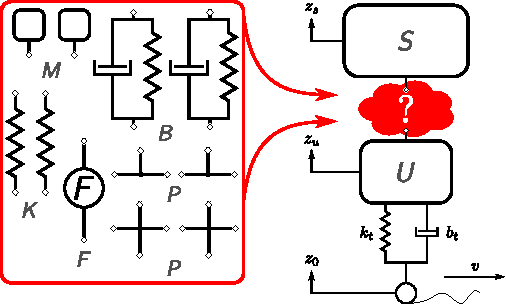
\includegraphics[width=0.6\columnwidth]{../ch2/figures/suspension1}
\caption{Suspension architecture enumeration case study.\label{fig:ch2:suspension1}}
\end{figure}

A graph representing a quarter-car suspension was introduced in Fig.~\ref{fig:ch2:initialexamples1}; now we will seek graphs that have different topologies between the sprung ($\xcolor{S}$) and unsprung ($\xcolor{U}$) masses represented in Fig.~\ref{fig:ch2:suspension1}. These graphs could then be used with design studies that evaluate the performance of a particular suspension architecture (see Ref.~\cite{Allison2014b} for a design study on a particular architecture).
The components considered will be additional masses, springs, dampers, a force actuator, and parallel connections (these are schematically shown in Fig.~\ref{fig:ch2:suspension1}). The specific selection of $(C,R,P)$ was chosen to be near the limits of what is currently possible with the proposed enumeration methods in this article.

Some additional assumptions are also made on the component definitions. First, $\xcolor{B}$ is a parallel damper and spring to ensure that there is a stable equilibrium point for the damper. Next, both 3- and 4-port parallel components are included to facilitate more efficient generation of the useful architectures. A 4-port parallel connection is equivalent to two 3-port parallel connections but the 4-port component provides structure that can be utilized with some specific NSCs. With the problem outlined, the base three-tuple is specified as:
\begin{gather*}
{C} = \{ \xcolor{S}, \xcolor{U}, \xcolor{M}, \xcolor{K}, \xcolor{B}, \xcolor{F}, \xcolor{P}, \xcolor{P} \}, \quad R =  [1,1,2,2,2,1,2,2] \\
{P} = [1,1,1,2,2,2,3,4], \quad N_P = 28, \quad N_C = 13 \\
1.01 \times 10^{7} \leq \abs*{\mathcal{G}_3} \leq 2.13 \times 10^{14}
\end{gather*}

The NSCs for this case study are now listed with expanded details on reduced potential adjacency matrix $A_R$. A few of the constraints utilize insights from the physical modeling of the suspension architectures.

\begin{enumerate}[label=$\bullet$, widest=$\bullet$, nosep]

\item \ref{ch2:s1}, \ref{ch2:s3} and \ref{ch2:s4} with $M = [1, 1, 0, 0, 0, 0, 0, 0]$ enforcing that both the sprung and unsprung masses must be connected and all components not connected to these two are removed.

\item \ref{ch2:s7} with $P$ as the number of unique edges.

\item $A_R(2,1) = 0$ for \ref{ch2:s5} to avoid a direct connection between the sprung and unsprung masses as it would defeat the purpose of a suspension to isolate the masses. If this constraint was not added, $1/27$ of graphs generated from a pure \mypm{} approach would contain this connection.

\item $A_R(3,1) = A_R(3,2) = 0$ for \ref{ch2:s5} since a feasible graph cannot have either $\xcolor{S}$ or $\xcolor{U}$ be connected to $\xcolor{M}$ as there would not be a path between between $\xcolor{S}$ and $\xcolor{U}$. Therefore, no unique graphs are lost with this constraint. Rather, a more efficient enumeration results.

\item $A_R(8,8) = A_R(7,7) = A_R(8,7) = 0$ for \ref{ch2:s5} so no parallel components can be connected to each other. This greatly reduces the number of graphs generated by providing some specific structure on the number and type of parallel connections in the architectures.

\item $A_R(4,4) = A_R(5,5) = 0$ for \ref{ch2:s5} so no two $\xcolor{K}$ or $\xcolor{B}$ components can be connected in series since there are straightforward relationships to combine these series elements into a single equivalent component. By eliminating this type of connection when generating graphs, we have a substantially smaller number of graphs to evaluate.

\item No parallel connection path can exist between a connected $\xcolor{S}$ or $\xcolor{U}$ as these masses would not be isolated. This is slightly different than the NSCs in Sec.~\ref{sec:ch2:NSC} and is checked after \ref{ch2:s5}.

\item Cycles appear with single parallel components where the components in the cycle would not appear in the dynamic model based on the properties of a parallel connection (e.g.,~with the cycle \resizebox{!}{0.03\columnwidth}{
\begin{tikzpicture}[
mynode/.style={draw, circle, very thick, inner sep=0.1pt, scale=1.3},
myline/.style={draw, very thick},
]
\node[mynode,draw=none] (1) at (0,0) {$\xcolor{P}$};
\node[mynode,draw=none] (2) at (0.8,0.3) {$\xcolor{K}$};
\node[mynode,draw=none] (3) at (1.6,0)  {$\xcolor{B}$};
\draw [myline] (1) -- (2);
\draw [myline] (1) -- (3);
\draw [myline] (2) -- (3);
\end{tikzpicture}}
, neither $\xcolor{K}$ nor $\xcolor{B}$ would appear in the dynamic model). Graphs with these cycles are declared unuseful since an isomorphic graph with the parallel cycle removed would already appear in the set of graphs generated by the tree algorithm.

\item Many series connections between the 2-port components are interchangeable (e.g.,~$\xcolor{F}-\xcolor{K}$ and $\xcolor{K}-\xcolor{F}$ in series are physically equivalent). Therefore, these interchangeable series components are combined into a single equivalent component type (modifying the graph) and checked for isomorphisms. For the previously mentioned example, the equivalent component type would be $\xcolor{FK}$ based on alphabetical ordering of the original component labels.

\end{enumerate}

The complete $A_R$ is shown in Fig.~\ref{fig:ch2:suspension2_1} and its expansion to the potential adjacency matrix in Fig.~\ref{fig:ch2:suspension2_2} noting that both of these matrices are symmetric. Figure~\ref{fig:ch2:suspension2_2} has $1$s on the diagonal since self-connections should be allowed so the desired graph structure space is covered. For example, we might want to consider graphs where all components are present except a single $\xcolor{K}$ component and this only can occur if the detached $\xcolor{K}$ is connected to itself (and later removed).

\begin{figure}
\centering
\begin{subfigure}[b]{\columnwidth}
\centering
\begin{align*}
% \scalemath{0.7}{
\scalemath{0.9}{
\begin{blockarray}{ccccccccc}
& \xcolor{S} & \xcolor{U} & \xcolor{M} & \xcolor{K} & \xcolor{B} & \xcolor{F} & \xcolor{P} & \xcolor{P} \\
\begin{block}{c[cccccccc]}
\xcolor{S} & 1 & \cdot & \cdot & \cdot & \cdot & \cdot & \cdot & \cdot \\
\xcolor{U} & \hlight{0}{20} & 1 & \cdot & \cdot & \cdot & \cdot & \cdot & \cdot \\
\xcolor{M} & \hlight{0}{55} & \hlight{0}{55} & 1 & \cdot & \cdot & \cdot & \cdot & \cdot  \\
\xcolor{K} & 1 & 1 & 1 & \hlight{0}{90} & \cdot & \cdot & \cdot & \cdot  \\
\xcolor{B} & 1 & 1 & 1 & 1 & \hlight{0}{90} & \cdot & \cdot & \cdot  \\
\xcolor{F} & 1 & 1 & 1 & 1 & 1 & 1 & \cdot & \cdot  \\
\xcolor{P} & 1 & 1 & 1 & 1 & 1 & 1 & \hlight{0}{37.5} & \cdot \\
\xcolor{P} & 1 & 1 & 1 & 1 & 1 & 1 & \hlight{0}{37.5} & \hlight{0}{37.5} \\
\end{block}
\end{blockarray}
}
\end{align*}
% \vspace{-0.35in}
\caption{Reduced potential adjacency matrix $A_R$.\label{fig:ch2:suspension2_1}}
% \vspace{0.1in}
\end{subfigure}
% 
\begin{subfigure}[b]{\columnwidth}
\vspace{0.3in}
\centering
\begin{align*}
% \scalemath{0.7}{
\scalemath{0.9}{
\begin{blockarray}{cccccccccccccc}
& \xcolor{S} & \xcolor{U} & \xcolor{M} & \xcolor{M} & \xcolor{K} & \xcolor{K} & \xcolor{B} & \xcolor{B} & \xcolor{F} & \xcolor{P} & \xcolor{P} & \xcolor{P} & \xcolor{P} \\
\begin{block}{c[ccccccccccccc]}
\xcolor{S} & \tikzmark{top}{1} & \cdot & \cdot & \cdot & \cdot & \cdot & \cdot & \cdot & \cdot & \cdot & \cdot & \cdot & \cdot \\
\xcolor{U} & \hlight{0}{20} & 1 & \cdot & \cdot & \cdot & \cdot & \cdot & \cdot & \cdot & \cdot & \cdot & \cdot & \cdot \\
\xcolor{M} &	\hlight{0}{55} & \hlight{0}{55} & 1 & \cdot & \cdot & \cdot & \cdot & \cdot & \cdot & \cdot & \cdot & \cdot & \cdot \\
\xcolor{M} &	\hlight{0}{55} & \hlight{0}{55} & 1 & 1 & \cdot & \cdot & \cdot & \cdot & \cdot & \cdot & \cdot & \cdot & \cdot \\
\xcolor{K} &	1 & 1 & 1 & 1 & 1 & \cdot & \cdot & \cdot & \cdot & \cdot & \cdot & \cdot & \cdot \\
\xcolor{K} &	1 & 1 & 1 & 1 & \hlight{0}{90} & 1 & \cdot & \cdot & \cdot & \cdot & \cdot & \cdot & \cdot \\
\xcolor{B} &	1 & 1 & 1 & 1 & 1 & 1 &	1 & \cdot & \cdot & \cdot & \cdot & \cdot & \cdot \\
\xcolor{B} &	1 & 1 & 1 & 1 & 1 & 1 &	\hlight{0}{90} & 1 & \cdot & \cdot & \cdot & \cdot & \cdot \\
\xcolor{F} &	1 & 1 & 1 & 1 & 1 & 1 &	1 & 1 & 1 & \cdot & \cdot & \cdot & \cdot \\
\xcolor{P} &	1 & 1 & 1 & 1 & 1 & 1 &	1 & 1 & 1 & 1 & \cdot & \cdot & \cdot \\
\xcolor{P} &	1 & 1 & 1 & 1 & 1 & 1 &	1 & 1 & 1 & \hlight{0}{37.5} & 1 & \cdot & \cdot \\
\xcolor{P} &	1 & 1 & 1 & 1 & 1 & 1 & 1 &	1 & 1 & \hlight{0}{37.5} & \hlight{0}{37.5} & 1 & \cdot \\
\xcolor{P} &	1 & 1 & 1 & 1 & 1 & 1 & 1 & 1 &	1 & \hlight{0}{37.5} & \hlight{0}{37.5} & \hlight{0}{37.5} & \tikzmark{bottom}{1}\ \\
\end{block}
\end{blockarray}
}
\end{align*}
\caption{Potential adjacency matrix.\label{fig:ch2:suspension2_2}}
\end{subfigure}
\caption{Suspension case study matrices for \ref{ch2:s5} and the tree search algorithm.\label{fig:ch2:suspension2}}
\end{figure}

The results are presented in similar manner to the previous case studies: $4.7\times 10^{21}$ adjacency matrices\footnote{This represents the fairest comparison as the proper permutations of the ports representation of the potential adjacency matrix in Fig.~\ref{fig:ch2:suspension2_2} without the parallel components. There are $5.4 \times 10^8$ adjacency matrices with a component representation but this suffers from the unknown parallel connection issue discussed in Sec.~\ref{sec:ch2:candidates}. There are $3.0 \times 10^{23}$ adjacency matrices directly using the matrix in Fig.~\ref{fig:ch2:suspension2}b.} ($\mathcal{G}_0$); $2.1 \times 10^{14}$ \mypm{}s ($\mathcal{G}_1$); $1.6 \times 10^8$ candidate graphs generated through the basic tree search algorithm; $3.2 \times 10^7$ remaining candidate graphs after initial port-type isomorphism filter; $1.9 \times 10^6$ feasible graphs ($\mathcal{G}_2$); and 13,727 unique graphs ($\mathcal{G}_3$). $2\times 10^{9}$ graph comparisons were needed and $3 \times 10^7$ required a full isomorphism check.
Two unique architectures are shown in Fig.~\ref{fig:ch2:suspension3} with Fig.~\ref{fig:ch2:suspension3_1} being a common architecture \cite{Allison2014b}.

\begin{figure}
\centering
\begin{subfigure}[b]{0.3\columnwidth}
\centering
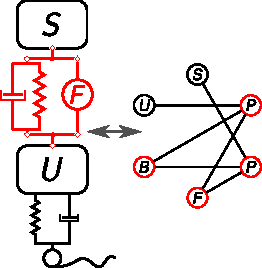
\includegraphics[width=\columnwidth]{../ch2/figures/suspension3_1}
\caption{\mypm{}~49073434464833.\label{fig:ch2:suspension3_1}}
\end{subfigure}
\begin{subfigure}[b]{0.35\columnwidth}
\centering
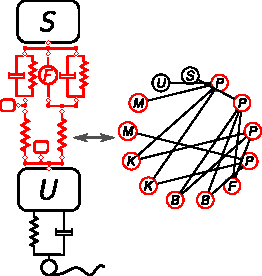
\includegraphics[width=\columnwidth]{../ch2/figures/suspension3_2}
\caption{\mypm{}~48728499790028.\label{fig:ch2:suspension3_2}}
\end{subfigure}
\caption{Two architectures for the suspension case study.\label{fig:ch2:suspension3}}
\end{figure}

%------------------
\section{Discussion}

It is clear in the case studies that the number of unique designs is much smaller than the upper bounds given by either permutations of the adjacency matrix or a \mypm{} approach. We also can directly visualize the effect of adding specific NSCs. NSCs limited the architecture design space, but in a predictable manner. One such example was not allowing parallel components to be connected together in \nameref{sec:ch2:example4}. A 5-port parallel connection was no longer possible (i.e.,~a 3-port and 4-port parallel components connected), but this NSC greatly reduced the number of graphs generated excluding many infeasible graphs, such as ones where parallel connection paths existed between a connected $\xcolor{S}$ or $\xcolor{U}$. Therefore, the addition of this NSC was a decision based on the tradeoff between  coverage of the architecture design space and efficiency.
\nameref{sec:ch2:example4} also demonstrated that fairly large problem sizes can be enumerated with the improved tree search algorithm provided enough constraints are present. Also, all possible subgraphs that are connected and complete appear in the set of unique designs without any NSCs (e.g.,~all graphs in Fig.~\ref{fig:ch2:unique2} appear as subgraphs in Fig.~\ref{fig:ch2:unique1}).

All reported unique solutions have a corresponding \mypm{} number. This number may not be unique since other \mypm{} numbers maybe isomorphic to the resulting $G^{CC}$. We see an example of two different \mypm{}s producing isomorphic graphs (\mypm{}~462 in Fig.~\ref{fig:ch2:model1_4} and \mypm{}~678 in Fig.~\ref{fig:ch2:unique1:g}).
While checking for isomorphisms can be computationally demanding, there typically is only a small subset of graphs that need the full isomorphism check as many comparisons fail with the simple checks and filters. Algorithm~\ref{alg:ch2:cip} can be useful to any architecture design problem no matter how the set of colored graphs is generated.
Many of the results and algorithms assumed simple components, but structured components (i.e.,~a planetary gear) can be readily included. Replacing a simple component type with an equivalent structured component type would simply have the effect of increasing the number of unique designs.

The previous sections only considered enumeration constructing a specific graph structure space. However, many problems are too large for the proposed enumeration algorithms because computational limits (e.g.,~memory needed to store the graphs and computation time of Alg.~\ref{alg:ch2:cip}) and evaluation limits (i.e., too many graphs are generated and we cannot evaluate all of them). Therefore, we need to consider methods that provide suitable \textit{exploration} of the desired design space.

Both the pure \mypm{} approach and the tree search algorithms have nice properties such as the high likelihood of producing feasible, nonisomorphic graphs while not limiting the design space. A stochastic sampling of the unique integers between 1 and $\mathcal{D}(N_P)$ can produce any arbitrary number of \mypm{} graphs. However, more structured sampling approaches may be preferred. Consider the unique graphs in Fig.~\ref{fig:ch2:unique1}. We could have tested all \mypm{}s between 227 to 913 and found all unique graphs. A \mypm{} approach does exhibit some interesting similarly-preserving properties (e.g.,~the graphs for a given \mypm{} number and the next integer value have a high likelihood of containing similar edges). Further exploration of the structural properties of \mypm{} graphs could lead to better sampling techniques that still cover the desired design space.

We can further consider ways to structure the exploration space with the coupon collector's problem. This problem, stated in a form relevant to this article, is: 
\begin{quote}
There are $n$ unique graphs and at each trial, a new graph is chosen at random (with replacement). Let $m$ be the number of trials. What is the expected number of trials such that all $n$ unique graphs are selected?
\end{quote}

\noindent The expected number of trials needed grows as $O(n\ln(n))$ \cite{Flajolet1992a}. Some of the assumptions in the problem are not directly satisfied such replacement and the probability distribution of choosing a particular unique graph but further study on the structure of $\mathcal{G}_1$ may yield exploration that `collects' most of the unique graphs in a more efficient manner.

The tree search algorithms may also be used for exploration. On Line~\ref{alg:ch2:cip:5} of Alg.~\ref{alg:ch2:cip}, we can randomly select an edge to add from $\xvar{I}$ instead of trying all possible edges. Therefore, the tree can be explored stochastically. Since the number of branches from a leaf varies, the probability of arriving at a certain final edge set is not equal (these probabilities can be calculated by assuming the tree is a Markov chain). Since the tree search algorithms cover the same desired graph structure space as the pure \mypm{} approach, can we selectively sample the tree and have some predictions on when all unique designs are found? These questions are left as future work items. 

Finally, it is important to describe the specific uses of the proposed algorithms. They are suitable for problems that are represented by undirected colored graphs under the component/port paradigm \cite{Mittal1989a, Snavely1993a, Munzer2013a}.
Enumeration is appropriate for certain problem classes (primarily determined by size). It may also be appropriate for searching for all possible enhancing structures \cite{Munzer2013a}. Enumeration has been useful for generating lists of organic molecules \cite{Carhart1975a, Faulon2003b, Ruddigkeit2012a}, finding all geometries of electrical circuits \cite{Foster1932a}, identifying all biological network architectures that achieve specific behaviors \cite{Ma2009a}, enumerating different gear trains \cite{Pennestri2015a, Castillo2002a}, and determining all hybrid powertrain configurations for a set list of components \cite{Bayrak2016a}.

Exploration is suitable for sampling the design space for much larger problems \cite{Wyatt2014a}. These samples could be used as visualizations for expert evaluation or starting points for generative approaches. The unrestricted graphs from a \mypm{} approach could also be used in conjunction with feature extraction algorithms to develop generative rules that are not based solely on experience and intuition (where the features are subgraphs that provide desired benefits to the architecture) \cite{Berlingerio2009a}.

%------------------
\section{Summary}

Architecture design is a challenging problem and this chapter presents some theory for generating candidate architectures with perfect matchings.
A \mypm{} approach is a graph numerical representation scheme that completely covers the design space that is needed in many architecture design problems.
It ensures certain frequency and degree requirements are met on specific list of potential components.
Enumeration of architecture design spaces can provide coverage and insights not currently possible with generative design approaches since enumeration approaches allow the designer to make specifications that they understand such as constraints and potential components, rather than rules for how things should be connected.

% new paragraph
A number of general network structure constraints are fully outlined with the specifics of checking their satisfaction with available graph analysis tools.
The colored graph isomorphism problem is discussed in great detail including the distinction between port-type and component-type isomorphisms.
The limited number of full isomorphism checks and the efficiency of Alg.~\ref{alg:ch2:cip} demonstrate that larger than expected architecture design spaces can be obtained.
A basic and improved tree search algorithm that avoids port-type isomorphisms was shown and is a primary example of how constraints can be naturally satisfied without reducing the design space.

% new paragraph
The various case studies are initial insights into the true nature of the class of architecture problems studied in this dissertation.
Consider again that there are only 12 unique graphs in Fig.~\ref{fig:ch2:unique3} of 2,097,152 adjacency matrices and 135,135 \mypm{}s.
For the suspension case study, a wide variety of network structure constraints were included based on natural requirements such as no direct connection between the sprung and unsprung masses.
Other constraints were added to avoid duplicate dynamic models such as the avoidance of parallel cycles and series connections between the 2-port components.
Moreover, constraints based on the experience and intuition of the designer were also included which limited the design space in a predictable manner such as the requirement that no parallel components can be connected together.

% new paragraph
Future graph generation algorithms can use these insights to suitably address the unique challenges associated with architecture design problems.
A number of directions are possible with the \mypm{} framework including deeper analysis of the structural properties of \mypm{} graphs, reduction of the number of graphs generated by the tree search algorithm, and the development of structured sampling approaches that result in nearly all unique graphs. % architecture
\mychapterfoot{Co-Design: Combined Plant and Control Design\label{ch:3}}

\footnotetext{Elements of this chapter are based on work completed in Ref.~\cite{Herber2017b}.
A published journal article (\href{https://doi.org/10.1115/1.4040705}{10.1115/1.4040705}) improves and expands on this chapter as described in the \nameref{ch:errata}.}

%--- epigraph
\epigraph{\textit{``If we want to solve problems effectively\dots we must keep in mind not only many features but also the influences among them. Complexity is the label we will give to the existence of many interdependent variables in a given system. The more variables and the greater their interdependence, the greater the system's complexity. Great complexity places high demands on a planner's capacity to gather information, integrate findings, and design effective actions.''}}{\textmd{D. D\"{o}rner} \cite[p.~38]{Dorner1997a}}
%--- epigraph

Many dynamic engineering system design problems contain two groupings of the design variables: plant (or artifact) and control.
For instance, consider again the system-level design of a robotic manipulator presented in Chapter~\ref{ch:1}. The plant design may comprise the geometric properties of the links and the control design may be embodied by the joint torque time trajectories for a specific task~\cite{Allison2013d}.
Many authors have shown the benefit of a combined strategy rather than a sequential approach~\cite{Fathy2003a, Allison2014b, Deshmukh2016a, Yan2009a, Fathy2001a}.
With a sequential approach, the plant is optimized initially, followed by the controller~\cite{Fathy2001a, Allison2014a}. 
In this chapter, we focus on two solution strategies appropriate for combined plant and controller design or co-design: \textit{simultaneous} and \textit{nested}.

% new paragraph
The simultaneous solution strategy optimizes both the plant and control variables in same optimization formulation.
With the nested strategy, an outer optimization loop optimizes the plant design, and an inner optimization loop identifies the optimal control for each plant design tested by the outer loop~\cite{Fathy2001a, Allison2014a}.
These two strategies are selected for a few reasons beyond them being the most studied and used in the literature.
First, the simultaneous strategy is the most fundamental representation of an integrated design problem \cite{Martins2013a}. 
On the other hand, the nested strategy is a specific reorganization of the optimization problem based on the plant and control disciplines.
Multidisciplinary design optimization (MDO) is a field of research that investigates design methods for systems with multiple disciplines \cite{Martins2013a, Allison2014a}.
However, if we are limited to single-system problems and implementations that do not partition the system across trajectories, there are a limited number of appropriate MDO methods suitable for co-design.
One reason for this is that many MDO formulations were developed in a way that does not explicitly address the dynamic nature of general co-design problems \cite{Allison2014a}.
This has led to partitioning schemes without full consideration of the coupling in the system.
Allison and Nazari developed an augmented Lagrangian coordination method for co-design, but only accounted for unidirectional (plant) coupling \cite{Allison2010b}.
The nested approach naturally handles single-system problems, bidirectional coupling, and the various trajectories in the problem.
Another important motivating reason for reorganizing the original problem is to employ specialized optimization algorithms to solve specific subproblems \cite{Allison2010b, Kusiak1995a}.
A number of efficient solution methods for specific problem forms can be utilized with the nested strategy.
However, as it will be discussed throughout this article, both of these strategies have their drawbacks. 
Many of these issues are well known for simultaneous strategy, motivating the fields of MDO and distributed optimization \cite{Martins2013a}.
The nested strategy is not amenable to coarse-grained parallelism and can be computationally intensive \cite{Allison2010b}.
Additionally, it can have potential feasibility issues.

% new paragraph
Here we consider co-design problems that are well-posed as \glsfirst{DO} problems~\cite{Fathy2001a, Allison2014a, Herber2014a}.
Co-design theory has focused primarily on specific DO formulations; as a result, only limited types of co-design problems fit into the existing frameworks.
With a specific problem structure, a variety of algorithms have been developed to provide numerical solutions, and detailed analysis of the coupling and partitioning has been investigated~\cite{Fathy2001a, Frischknecht2011a, Reyer2001a, Hale1985a, Eastep1987a, Sunar1993a, Peters2011a, Peters2009a}.
Such works have made considerable progress towards addressing specific challenges found in certain co-design problems.
However, there has been less attention towards the general co-design problem (i.e.,~a co-design formulation with no restrictions) perhaps due to the lack of efficient solution techniques and continuing legacy design practices that treat certain problem elements as naturally separate~\cite{Allison2014a}. 

% new paragraph
Recently, numerical solution methods have been utilized to solve co-design problems that are not captured by previous problem definitions~\cite{Allison2014a, Herber2014a}.
Nontraditional problem formulation elements include system-level objective functions, general inequality path constraints, and general boundary conditions~\cite{Allison2013d, Allison2014b, Deshmukh2016a, Fathy2003a, Herber2013a, Maraniello2016a, Yan2009a, Chilan2017a}.
With these nontraditional problem elements, much of the previous work in co-design theory does not apply.
An essential element of engineering design optimization is an appropriate problem formulation.
A thorough analysis of the general co-design formulation is needed to better allow designers to leverage the advantages intrinsic to the co-design methodology.

% new paragraph
One of the numerical solution methods recently applied to co-design problems is known as \glsfirst{DT}, which approximates the infinite-dimensional DO problem with a finite \glsfirst{NLP} that can be solved with standard NLP solvers~\cite{Betts2010a, Biegler2010a, Rao2010a, Allison2014b}. 
DT has a number of favorable properties that supports the efficient generation of solutions to general co-design problems~\cite{Allison2014a, Allison2014b, Herber2014a}.

% new paragraph
In this chapter, we will explore the general co-design problem with a focus on the simultaneous and nested solution strategies.
Section~\ref{sec:ch3:formulation} provides the formulations for the simultaneous and nested co-design solution strategies and Sec.~\ref{sec:ch3:conditions} outlines the necessary conditions for optimality for both.
Section~\ref{sec:ch3:numerical} discusses some practical solution considerations relevant to the two strategies.
Section~\ref{sec:ch3:casestudies} presents a number of test problems and finally, Sec.~\ref{sec:ch3:conclusion} offers a summary.

\section{Problem Formulation \label{sec:ch3:formulation}}

Here we  present the two co-design strategies. First, we state a few assumptions. Initially, the time horizon $t_{\glsfirst{initial}} \leq \gls{time} \leq t_{\glsfirst{final}}$ is assumed to be fixed. Section~\ref{sec:ch3:time} discusses the inclusion of the horizon boundaries in the co-design problem formulations.
Next, only general inequality constraints will directly appear in the formulations for conciseness of the formulations. Equality constraints are captured by two inequality constraints (i.e.,~$\glsfirst{f}(\gls{x}) = 0$ is equivalent to $f(\bm{x}) \leq 0$ and $-f(\bm{x}) \leq 0$). % cite something?

\subsection{Simultaneous Formulation}

The general simultaneous co-design problem formulation contains all relevant objectives and constraints in a single optimization formulation. % AAO?
The DO problem formulation is:
\begingroup
\allowdisplaybreaks
\begin{subequations}
\label{eq:simprob}
\begin{align}
\min_{\bxp, \bxc} \quad & \Psi(\bxp, \bxc) = \int_{t_0}^{t_f} \lagrange \left( t, \bxi, \bxc, \bxp \right) dt \ + \cdots \label{eq:ch3:sim_lagrange} \\
& \qquad \mayer \left( \bxi(t_0), \bxi(t_f), \bxc, \bxp \right) \label{eq:ch3:sim_mayer} \\
\text{subject to:} \quad & \dot{\bxi \glsfirst{timederiv}} - \bfd \left( t, \bxi, \bxc, \bxp \right) = \bzero \label{eq:ch3:sim_codesign_dyn} \\
& \gls{path} \left( t, \bxi, \bxc, \bxp \right) \leq \bzero \label{eq:sim_codesign_path} \\
& \gls{boundary} \left( \bxi(t_0), \bxi(t_f), \bxc, \bxp \right) \leq \bzero \label{eq:ch3:sim_codesign_bound}
\end{align}
\end{subequations}%
\endgroup

\noindent where $\bm{x}_{\glsfoo[noindex]{plant}}$ are the plant variables, $\bm{x}_{\glsfoo[noindex]{control}}$ are the control variables, $t$ is the time continuum defined between $t_0$ and $t_f$, $\gls{states}$ are the states, $\gls{objective}$ is the objective function in Bolza form, \gls{lagrange} is the Lagrange (running cost) term, \gls{mayer} is the Mayer (terminal cost) term, Eqn.~(\ref{eq:ch3:sim_codesign_dyn}) enforces the dynamics modeled as a first-order ordinary differential equation, Eqn.~(\ref{eq:sim_codesign_path}) enforces any time-varying path constraints, and Eqn.~(\ref{eq:ch3:sim_codesign_bound}) enforces any time-dependent constraints. See Ref.~\cite{Herber2014a} for a general discussion of this co-design formulation and the problem elements.

\subsection{Nested Formulation}

The alternative solution strategy to the simultaneous formulation in Prob.~(\ref{eq:simprob}) is a nested one where an outer optimization loop optimizes the plant design, and an inner optimization loop identifies the optimal control for each plant design tested by the outer loop.
Figure~\ref{fig:ch3:strategies} illustrates the two strategies.
This is a two-level optimization problem (a subclass of bilevel optimization)~\cite{Colson2007a, Vicente1994a, Tanino1984a}. The outer-loop problem is defined as:
\begin{subequations}
\label{eq:ch3:outerloop}
\begin{align}
\min_{\bxp} \quad & \psi ( \bxp ) \qquad \qquad \qquad \label{eq:ch3:outerloop_obj}
\end{align}
\vspace*{-\baselineskip}
\begin{empheq}[right={\empheqrbrace = \bm{g}_{o} ( \bxp ) \leq \bm{0} }]{align}
\text{subject to:} \quad & \bm{\phi}_{o} \left( \bxp \right) \leq \bzero \label{eq:ch3:outerloop_phi} \\
& \bm{F}(\bxp) \leq \bm{0} \label{eq:ch3:outerloop_F}
\end{empheq}
\end{subequations}

\begin{figure}[t]
\centering
\begin{subfigure}[b]{0.3\columnwidth}
       \centering
       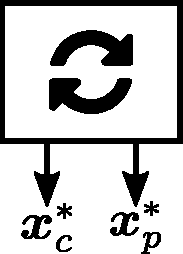
\includegraphics[width=0.46923076922in]{../ch3/figures/strategies_sim}
       \caption{Simultaneous strategy.\label{fig:ch3:strategies_sim}}
\end{subfigure}% 
\begin{subfigure}[b]{0.3\columnwidth}
       \centering
       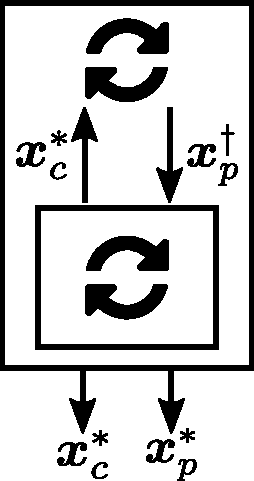
\includegraphics[width=0.65in]{../ch3/figures/strategies_nested}
       \caption{Nested strategy.\label{fig:ch3:strategies_nested}}
\end{subfigure}% 
\caption[Two co-design solution strategies]{Two co-design solution strategies where \faRefresh~indicates an optimization problem.\label{fig:ch3:strategies}}
\end{figure}

\noindent where $\bm{\phi}_{\glsfirst{outer}}$ are the constraints in $\bm{\phi}$ that only depend on the plant design, $\gls{inequality}_{o}$ is the collection of the outer-loop constraints, and $\{ \gls{objectiveouter} ( \bxp ), \gls{outerfeas}(\bxp) \}$ are two new problem formulation elements that will be outlined after the following inner-loop formulation:
\begin{subequations}
\label{eq:ch3:innerloop}
\begin{align}
\min_{\bxc} \quad & \Psi( \bxp^{\dagger}, \bxc) \qquad \qquad \qquad \qquad \qquad \quad
\end{align}
\vspace*{-\baselineskip}
\begin{empheq}[right={\empheqrbrace = \bm{g}_{i}\left( \cdot \right) \leq \bm{0} }]{align}
\text{subject to:} \quad &  \dot{\bxi} - \bfd \left( t, \bxi, \bxc, \bxp^{\dagger} \right) = \bzero \\
& \bm{C} \left( t, \bxi, \bxc, \bxp^{\dagger} \right) \leq \bzero \\
& \bm{\phi}_{i} \left( \bxi(t_0), \bxi(t_f), \bxc, \bxp^{\dagger} \right) \leq \bzero
\end{empheq}
\end{subequations}

\noindent where $\bxp^{\glsfirst{candidate}}$ is a candidate plant design, $\bm{\phi}_{\glsfirst{inner}}$ are the constraints of $\bm{\phi}$ not in $\bm{\phi}_{o}$, and $\bm{g}_{i}$ is the collection of the inner-loop constraints. With both formulations presented, some additional concepts relevant to two-level optimization problems need to be discussed.

% new paragraph
The simultaneous method's feasible set (or constraint region) is defined as:
\begin{align}
\gls{Omega} = \left\lbrace (\bxp, \bxc)\ :\ \bm{g}_{o}(\bxp, \bxc) \leq \bm{0}, \ \bm{g}_{i}(\bxp, \bxc) \leq \bm{0} \right\rbrace
\end{align}

\noindent For each candidate $\bxp^{\dagger}$, the inner-loop feasible set is defined by:
\begin{align}
\Omega(\bxp^{\dagger}) = \left\lbrace \bxc\ : \ \bm{g}_{i}(\bxp^{\dagger}, \bxc) \leq \bm{0} \right\rbrace
\end{align}

\noindent and then set of potential inner-loop optimal control designs is:
\begin{align}
\gls{Mcontrols}(\bxp^{\dagger}) = \left\lbrace \bxc\ :\ \bxc \in \arg\min \left\lbrace \Psi(\bxp^{\dagger}, \bxc)\ :\ \bxc \in \Omega(\bxp^{\dagger})  \right\rbrace \right\rbrace
\end{align}

\noindent For a given $\bxp$, $M(\bxp)$ may be empty for some values of its argument, i.e.,~no feasible control design exists for the given $\bxp$. If $\bxc \in M(\bxp)$, then the optimal objective function value from the inner loop is:
\begin{align}
\psi(\bxp) = \Psi(\bxp, \bxc)
\end{align}

\noindent which is used as the objective function of the outer loop, Eqn.~(\ref{eq:ch3:outerloop_obj}). Finally, the feasible set of the outer loop (known as the induced region) is:
\begin{align}
\gls{induced} = \left\lbrace (\bxp, \bxc)\ :\ (\bxp, \bxc) \in \Omega,\ \bxc \in M(\bxp) \right\rbrace
\end{align}

\noindent and we note that $\Omega$ and $I$ are not the same feasible region. This is the motivation behind the addition of Eqn.~(\ref{eq:ch3:outerloop_F}). $\bm{F}(\bxp)$ is an additional constraint that may be added to ensure for all $\bxp^{\dagger}$, $\Omega(\bxp^{\dagger})$ is nonempty, termed the outer-loop feasibility constraint. The two formulations are only equivalent if $\Omega$ remains unchanged. This constraint will be discussed more in the following discussion section.

\subsection{Formulation Discussion\label{sec:ch3:form_dis}}

Here we  discuss the specific problem formulation elements of both approaches, focusing on comparisons to the current co-design literature.

\subsubsection{Control Design Variables}

While plant variables will always be time-independent, control variables may be either time-independent or infinite-dimensional trajectories (with respect to time). We partition the control variables into two sets as:
\begin{align}
\bxc = \begin{bmatrix} \bp \\ \bu \end{bmatrix}
\end{align}

\noindent where \gls{parameters} are the control parameters and \gls{olc} are the \glsfoo[noindex]{OLC} variables.
The control parameters are static (time-independent) control variables (e.g.,~gains).
The OLC variables are infinite-dimensional trajectories through time (e.g.,~joint torque time profile for a robotic manipulator).
Both types of control design variables are found in the literature, although both types are not typically in the same design problem.
Even if there are no OLC variables, the general co-design problem is still an infinite-dimensional problem due to the dynamic and path constraints.
One very special case is when the optimal OLC can be defined with static gains such as with infinite-horizon \glsfirst{LQR}~\cite{Liberzon2012a, Belvin1990a, Rao1988a} discussed later in Sec.~\ref{sec:ch3:lqr}.
See Refs.~\cite{Belvin1990a, Eastep1987a, Fathy2003a, Rao1988a, Sunar1993a, Yan2009a} for examples with $\bp$ and Refs.~\cite{Allison2014b, Deshmukh2016a, Herber2013a, Maraniello2016a, Chilan2017a} for examples with $\bu$.

% paragraph about objective function
\subsubsection{Objective Function} 

Even though the objective function  is partitioned in Eqns.~(\ref{eq:ch3:sim_lagrange}) and (\ref{eq:ch3:sim_mayer}), converting between the Lagrange and Mayer terms is possible~\cite{Liberzon2012a, Herber2014a}. Both forms are present to allow for more natural formulations of the problem (and to be consistent with the literature).

A common form of the co-design objective function is:
\begin{align} \label{eq:ch3:sep_objs}
\min_{\bxp, \bxc} \quad \Psi = w_p \Psi_p ( \bxp ) + w_c \Psi_c\left( \bxp, \bxc \right)
\end{align}

\noindent where $\{\Psi_p, \Psi_c\}$ are the plant and control objective functions and $\{\gls{weights}_p, w_c\}$ are objective weights~\cite{Fathy2001a}. 
While many co-design problems are appropriately partitioned with control and plant specific objective function terms~\cite{Frischknecht2011a, Fathy2003a, Hale1985a, Peters2009a, Peters2011a, Rao1988a, Reyer2001a, Sunar1993a}, others necessitate the general objective form in Eqns.~(\ref{eq:ch3:sim_lagrange})--(\ref{eq:ch3:sim_mayer})~\cite{Allison2013d, Deshmukh2016a, Fathy2003a, Herber2013a, Chilan2017a}. 
These general objectives may only include one term or terms that are typically only classified as ``control'' objective terms.

\subsubsection{Path and Boundary Constraints}%
Equations~(\ref{eq:sim_codesign_path}) and (\ref{eq:ch3:sim_codesign_bound}) could be further generalized into a single general constraint form, but the distinction is important for both the optimality conditions and the numerical approaches used to find solutions.
The difference is primarily based on time dependence. Therefore, path and boundary constraints could be more appropriately named time-dependent and time-independent constraints.

% new paragraph
Boundary constraints are common to many existing co-design formulations~\cite{Fathy2001a, Allison2014a, Herber2014a}.
Traditional plant-only constraints such geometry or mass constraints are time-independent constraints~\cite{Peters2009a, Peters2011a, Allison2014b, Rao1988a}.
Many co-design formulations explicitly require initial condition constraints, but some co-design problems have unknown initial conditions or periodic constraints~\cite{Herber2013a}.
Another set of boundary constraints is the kinematic relationships in
robotics~\cite{Spong2005a}. These constraints might require an algebraic variable that depends on the states (e.g.,~the end position of the robotic manipulator depends on the state joint angles and geometric plant variables). 

% new paragraph
More recently, general path constraints have been included in co-design problems and are infinite-dimensional constraints~\cite{Herber2014a, Allison2014a, Allison2014b, Allison2013d}. 
Many traditional engineering constraints can be formulated naturally as path constraints.
States or outputs often need to be constrained between allowable bounds such as temperature, position, force, pressure, deflection, stress, power, etc. 
These examples are typically inequality path constraints but equality path constraints are also possible, such as an automobile following a prescribed drive cycle or ensuring the steady-state optimal tip-speed ratio is followed by a horizontal axis wind turbine~\cite{Deshmukh2016a}.
The inclusion of path constraints is critical to the usefulness of many co-design studies.
Fathy et al. included mixed control-plant constraints:
\begin{align}
\bm{C}\left(t, \bm{u}(t), \bm{x}_p \right) \leq \bm{0}
\end{align}
\noindent 
but mixed state-control-plant constraints as in Eqn.~(\ref{eq:sim_codesign_path}) are needed to represent many of the engineering constraints mentioned above~\cite{Fathy2001a}.

\subsubsection{Outer-Loop Feasibility Constraint}

For the two solution strategies to be equivalent, $M(\bxp)$ must be nonempty for every candidate $\bxp$~\cite{Fathy2001a}. Introducing an appropriate outer-loop feasibility constraint is one technique to ensure this property is satisfied.

% new paragraph
Consider again the design of a robotic manipulator. For certain geometric configurations, the kinematics restrictions of the manipulator may be such that it is unable to reach the prescribed target.
To avoid a candidate $\bxp$ that has no feasible control solution, we could add a reachability constraint to $\bm{F}(\bxp)$~\cite{Allison2013d, Spong2005a}.
However, even with this additional constraint, mixed state-control-plant constraints may be present that cannot be satisfied with the given plant design, such as stress or deflections~\cite{Allison2013d}.
This example helps illustrate that for general co-design problems, these constraints can be quite difficult (or impossible) to determine.

% new paragraph
An important type feasibility constraint is the classic controllability property applicable to linear systems theory~\cite{Fathy2001a}.
Unfortunately, controllability is not sufficient to guarantee the nonemptiness of $\Omega(\bxp^{\dagger})$ for general co-design problems.
For example, if control bounds are provided, then it is not guaranteed that we can move between arbitrary initial and final positions in finite time.

% new paragraph
It is also important to note that this outer-loop feasibility constraint may not strictly be required to find the system-optimal solution using the simultaneous strategy.
Another strategy is to add a feasibility constraint that restricts $\Omega$ such that the desired property holds.
This is not ideal since there will be no guarantee that the nested strategy will produce the system-level optimum, but may be a necessity for certain co-design problems.
The implications of this will be discussed in the following sections.

%---------------------------------------------------------------------
\section{Necessary Conditions for Optimality \label{sec:ch3:conditions}}

In this section, we describe the necessary conditions for optimality for the two general co-design strategies from the previous section. Sufficient conditions will not be discussed directly, but are the Hamiltonian minimization conditions~\cite{Liberzon2012a, Chachuat2007a, Bryson1975a} or second-order conditions on the Lagrangian for finite-dimensional problems~\cite{Papalambros2017a}.
If a problem is singular, there may be additional sufficient conditions needed~\cite{Chachuat2007a, Bryson1975a}.
We also assume that the simultaneous co-design problem is well-posed, i.e.,~there exists a solution. See Refs.~\cite{Liberzon2012a, Chachuat2007a, Papalambros2017a} for discussions on constraint qualification, regularity, differentiability, and other relevant properties for a well-posed problem.
We begin with the conditions for the OLC design only.

\subsection{Open-Loop Control Design}

The optimal OLC design problem formulation is:
\begingroup
\allowdisplaybreaks
\begin{subequations}
\label{eq:ch3:ocsd}
\begin{align}
\min_{\bu} \quad & \Psi = \int_{t_0}^{t_f} \lagrange \left( t, \bxi, \bu \right) dt + \mayer \left( \bxi(t_0), \bxi(t_f) \right) \\
\text{subject to:} \quad & \dot{\bxi} - \bfd \left( t, \bxi, \bu \right) = \bzero \label{eq:ch3:ocsd_2} \\
& \bm{C} \left( t, \bxi, \bu \right) \leq \bzero \label{eq:ch3:ocsd_3} \\
& \bm{\phi} \left( \bxi(t_0), \bxi(t_f) \right) \leq \bzero \label{eq:ch3:ocsd_4}
\end{align}
\end{subequations}
\endgroup

\noindent which is a subformulation of Prob.~(\ref{eq:simprob}).
Similar to the Lagrangian in finite-dimensional optimization~\cite{Papalambros2017a, Liberzon2012a}, the infinite-dimensional constraints can be adjoined to the Lagrange term with time-varying Lagrange multipliers, creating the Hamiltonian of the problem:
\begin{align}
\gls{hamiltonian} &= \lagrange + \blambda^{\glsfirst{transpose}} \bfd + \bmu\tran \bm{C}
\end{align}

\noindent where $\gls{costates}(t)$ are the costates (multipliers for the state dynamics) and $\gls{multiplierpath}(t)$ are the multipliers for $\bm{C}$.

% new paragraph
With this control-only formulation, we can directly apply \glsfirst{PMP} with path constraints~\cite{Pontryagin1962a, Liberzon2012a, Chachuat2007a} to arrive at the following necessary conditions for optimality (note, \glsname{optimal} is used to denote an optimal value):
\begin{subequations}
\label{eq:ch3:ocsd_cond}
\begin{gather}
\dot{\blambda}^* = - \left[ \pd{H}{\bxi} \right]^* \label{eq:ch3:ocsd_cond_1} \\
\bzero = \left[ \pd{H}{\bu} \right]^* \label{eq:ch3:ocsd_cond_2} \\
0 = \left[ \bmu\tran \bm{C}\right]^*, \quad 0 = \left[ \bnu\tran \bm{\phi} \right]^* \label{eq:ch3:ocsd_cond_3} \\
\bmu^* \geq \bzero, \quad \bnu^* \geq \bzero \label{eq:ch3:ocsd_cond_4} \\
\bzero = \left[ \blambda + \pd{\mayer}{\bxi} + \bnu\tran \pd{\bm{\phi}}{\bxi} \right]_{t_0}^* \label{eq:ch3:ocsd_cond_5}, \quad 
\bzero = \left[ \blambda - \pd{\mayer}{\bxi} - \bnu\tran \pd{\bm{\phi}}{\bxi} \right]_{t_f}^*
\end{gather}
\end{subequations}

\noindent where \gls{multiplierbound} are the Lagrange multipliers for $\bm{\phi}$,
Eqn.~(\ref{eq:ch3:ocsd_cond_1}) is the {costate dynamics},
Eqn.~(\ref{eq:ch3:ocsd_cond_2}) is the {control stationarity condition},
Eqns.~(\ref{eq:ch3:ocsd_cond_3}) are the {complementary slackness conditions},
Eqns.~(\ref{eq:ch3:ocsd_cond_4}) are the {dual feasibility conditions}, and
Eqns.~(\ref{eq:ch3:ocsd_cond_5}) are the {initial and final time transversality conditions}.
The conditions in Eqn.~(\ref{eq:ch3:ocsd_cond}) are in addition to the constraints in Eqns.~(\ref{eq:ch3:ocsd_2})--(\ref{eq:ch3:ocsd_4}). The necessary conditions for both strategies can now be derived.

\subsection{Co-design---Simultaneous Strategy}

Here we will derive the simultaneous co-design optimality conditions only using PMP.
Others have derived the optimality conditions for similar co-design formulations.
See Ref.~\cite{Dolezal1981a} for early work outside the co-design context.
Fathy et al. utilized a combination of the \glsfirst{KKT} conditions and PMP~\cite{Fathy2001a}.

% new paragraph
Consider the following augmented state vector:
\begin{align}
\label{eq:ch3:augmented_states}
\gls{augstate} = \begin{bmatrix} \bxi \\ \bxp \end{bmatrix}, \quad \dot{\bm{\Theta}} = \begin{bmatrix} \bfd \\ \bzero \end{bmatrix}
\end{align}

\noindent with the replacement of all plant variables with $\bxp(t_0)$ and, therefore, no dependence on $\bxp(t_f)$. Now consider if unconstrained, the choice of initial and final states are, in effect, additional decision variables that can be modified to satisfy the optimality conditions.

% new paragraph
The $\bm{\xi}$-dependent terms in Eqn.~(\ref{eq:ch3:ocsd_cond}) are Eqns.~(\ref{eq:ch3:ocsd_cond_1}) and (\ref{eq:ch3:ocsd_cond_5}). Applying these conditions to the ``state'' plant variables, we have the following additional conditions:
\begin{subequations}
\begin{align}
-\dot{\blambda}^*_p &= \left[ \pd{H}{\bxp} \right]^* = \left[ \pd{\lagrange}{\bxp}  + \blambda\tran \pd{\bfd}{\bxp} + \blambda_p\tran \cancelto{0}{\pd{\dot{\bm{x}}_p}{\bxp}} + \bmu\tran \pd{\bm{C}}{\bxp} \right]^*
  \\
\bzero &= \left[ \blambda_p + \pd{\mayer}{\bxp} + \bnu\tran \pd{\bm{\phi}}{\bxp} \right]_{t_0}^*  \\
\bzero &= \left[ \blambda_p - \cancelto{0}{\pd{\mayer}{\bxp}} - \bnu\tran \cancelto{0}{\pd{\bm{\phi}}{\bxp}} \quad \right]_{t_f}^* = \blambda_p^*(t_f)
\end{align}
\end{subequations}

\noindent Now using the first fundamental theorem of calculus, we can combine these equations into a single condition:
\begin{subequations}
\begin{gather}
\blambda^*_p(t_f) = \blambda^*_p(t_0) + \int_{t_0}^{t_f} \dot{\blambda}^*_p dt \\
\hspace*{-0.08in} \bzero = \left[ \pd{\mayer}{\bxp} + \bnu\tran \pd{\bm{\phi}}{\bxp} \right]_{t_0}^* + \int_{t_0}^{t_f} \left[ \pd{\lagrange}{\bxp}  + \blambda\tran \pd{\bfd}{\bxp} + \bmu\tran \pd{\bm{C}}{\bxp} \right]^* \hspace*{-0.07in} dt \label{eq:ch3:opt_cond_xp_codesign}
\end{gather}
\end{subequations}

\noindent This condition is analogous to the condition found in other derivations of the optimality conditions~\cite{Fathy2001a, Dolezal1981a}.
Note that the other conditions in Eqn.~(\ref{eq:ch3:ocsd_cond}) remain unchanged.
Therefore, the simultaneous co-design optimality conditions are a combination of Eqn.~(\ref{eq:ch3:ocsd_cond}) and Eqn.~(\ref{eq:ch3:opt_cond_xp_codesign}):
\begingroup
\allowdisplaybreaks
\begin{subequations}
\label{eq:ch3:opt_cond_sim}
\begin{gather}
\dot{\blambda}^* = - \left[ \pd{H}{\bxi} \right]^*, \quad 
\bzero = \left[ \pd{H}{\bu} \right]^* \\
0 = \left[ \bmu\tran \bm{C}\right]^*, \quad 0 = \left[ \bnu\tran \bm{\phi} \right]^*, \quad \bmu^* \geq \bzero, \quad \bnu^* \geq \bzero \\
\bzero = \left[ \blambda + \pd{\mayer}{\bxi} + \bnu\tran \pd{\bm{\phi}}{\bxi} \right]_{t_0}^*, \quad
\bzero = \left[ \blambda - \pd{\mayer}{\bxi} - \bnu\tran \pd{\bm{\phi}}{\bxi} \right]_{t_f}^* \\
\hspace*{-0.08in} \bzero = \left[ \pd{\mayer}{\bxp} + \bnu\tran \pd{\bm{\phi}}{\bxp} \right]_{t_0}^* + \int_{t_0}^{t_f} \left[ \pd{\lagrange}{\bxp}  + \blambda\tran \pd{\bfd}{\bxp} + \bmu\tran \pd{\bm{C}}{\bxp} \right]^* \hspace*{-0.07in}  dt
\end{gather}
\end{subequations}
\endgroup

\subsection{Co-design---Nested Strategy}

We now derive the necessary conditions for the nested strategy where the outer-loop problem is defined in Prob.~(\ref{eq:ch3:outerloop}) and the inner loop in Prob.~(\ref{eq:ch3:innerloop}).
The inner-loop optimality conditions are defined in Eqn.~(\ref{eq:ch3:ocsd_cond}) with only OLC variables.
If the inner loop contains $\bp$, then the necessary conditions are analogous to the simultaneous conditions in Eqn.~(\ref{eq:ch3:opt_cond_sim}) with $\bp$ replacing $\bxp$.

% new paragraph
The outer-loop problem is finite-dimensional optimization since neither the dynamics nor path constraints are present. Therefore, we can directly utilize the KKT conditions~\cite{Papalambros2017a}. The Lagrangian for the outer-loop problem is:
\begin{align}
L = \psi + \gls{multiplierouter}\tran \bm{\phi}_o + \gls{multiplierfeas}\tran \bm{F}
\end{align}

\noindent We first express the stationarity condition:
\begin{subequations}
\label{eq:ch3:nested_stationarity}
\begin{align}
\bzero = \der{L}{\bxp} &= \der{\psi}{\bxp} + \bm{\chi}\tran \der{\bm{\phi}_o}{\bxp} + \bm{\eta}\tran \der{\bm{F}}{\bxp} \\
&= \int_{t_0}^{t_f} \der{\lagrange}{\bxp} dt + \der{\mayer}{\bxp} + \bm{\chi}\tran \der{\bm{\phi}_o}{\bxp} + \bm{\eta}\tran \der{\bm{F}}{\bxp}
\end{align}
\end{subequations}

\noindent Now the total derivative terms can be explicated~\cite{Weisstein2016a}:
\begin{subequations}
\begin{align}
\der{\lagrange}{\bxp} &= \pd{\lagrange}{\bxp} + \pd{\lagrange}{\bxi^*}  \der{\bxi^*}{\bxp} + \pd{\lagrange}{\bu^*} \der{\bu^*}{\bxp} + \pd{\lagrange}{\bp^*} \der{\bp^*}{\bxp} \\
\der{\mayer}{\bxp} &= \pd{\mayer}{\bxp} + \left[ \pd{\mayer}{\bxi^*}  \der{\bxi^*}{\bxp} \right]_{t_0} + \left[ \pd{\mayer}{\bxi^*}  \der{\bxi^*}{\bxp} \right]_{t_f} + \pd{\mayer}{\bp^*}  \der{\bp^*}{\bxp} \label{eq:ch3:total_der_mayer}
\end{align}
\end{subequations}

\noindent Here we see a number of coupled terms.

% new paragraph
The complete set of necessary conditions for the outer loop are then:
\begin{subequations}
\label{eq:ch3:nested_cond}
\begin{gather}
\bzero = \der{\Psi}{\bxp} + \bm{\chi}\tran \der{\phi_o}{\bxp} + \eta\tran \der{F}{\bxp} \\
\bm{\chi} \geq \bzero, \quad \bm{\eta} \geq \bzero, \quad 
\bm{\chi}\tran \bm{\phi}_o = \bzero, \quad \bm{\eta}\tran \bm{F} = \bzero
\end{gather}
\end{subequations}

\noindent which are a set of KKT conditions. The conditions in Eqn.~(\ref{eq:ch3:nested_cond}) are in addition to the constraints Eqns.~(\ref{eq:ch3:outerloop_phi}) and (\ref{eq:ch3:outerloop_F}).

\subsection{Free Time \label{sec:ch3:time}}

The initial and final time values can be optimization variables as well~\cite{Liberzon2012a, Chachuat2007a, Fathy2001a, Herber2014a}.  
Optimal control problems frequently contain these terms and therefore, appropriate optimality conditions are provided.
Subsequently, these additional optimization variables are typically included in the inner-loop problem of the nested co-design strategy~\cite{Fathy2001a}. 
However, some of the numerical methods used jointly with certain co-design strategies lose certain properties when the time horizon is not fixed.
In these situations, perhaps, it is more beneficial to place these additional variables in the outer loop to maintain such properties.

The simultaneous co-design strategy will need one additional equation if $t_f$ is free:
\begin{align}
0 = \left[\pd{\mayer}{t_f} + \bnu\tran \pd{\bm{\phi}}{t_f} \right]^* + \left[ \lagrange + \blambda\tran \bfd + \bmu\tran \bm{C} \right]^*_{t_f}
\end{align}

\noindent This is an additional transversality condition with the others in Eqn.~(\ref{eq:ch3:ocsd_cond_5})~\cite{Liberzon2012a, Chachuat2007a}.

For a nested approach with $t_f$ free in the outer loop, the additional stationary condition $d L / d t_f = 0$ would include: 
\begin{subequations}
\begin{align}
\der{\lagrange}{t_f} &= \pd{\lagrange}{t_f} + \pd{\lagrange}{\bxi^*}  \der{\bxi^*}{t_f} + \pd{\lagrange}{\bu^*} \der{\bu^*}{t_f} + \pd{\lagrange}{\bp^*} \der{\bp^*}{t_f} \\
\der{\mayer}{t_f} &= \pd{\mayer}{t_f} + \left[ \pd{\mayer}{\bxi^*}  \der{\bxi^*}{t_f} \right]_{t_0} + \left[ \pd{\mayer}{\bxi^*}  \der{\bxi^*}{t_f} \right]_{t_f} + \pd{\mayer}{\bp^*}  \der{\bp^*}{t_f}
\end{align}
\end{subequations}

This completes the necessary conditions for optimality for the various problem formulations and solution strategies.
Now some of the computational and practical aspects will be discussed.

%---------------------------------------------------------------------
\section{Practical Solution Considerations \label{sec:ch3:numerical}}

Obtaining solutions only using the optimality conditions in the previous section can be challenging. Practical formulation limitations, robustness, and computational efficiency also need to be considered when seeking solutions to co-design problems.

\subsection{Obtaining Approximate Solutions \label{sec:ch3:approx}}

In the previous section,  the finding an analytic solution that satisfies the optimality conditions is called an indirect method~\cite{Betts2010a, Biegler2010a}. Although this approach can lead to important insights into the structure of the solution, it can be quite challenging (or impossible) to solve these equations analytically.
If complicated black box functions or table interpolation is used, analytic forms for their derivatives do not even exist.
Therefore, numerical methods are often employed that provide approximate solutions to the original problem.

% new paragraph
Numeric indirect methods derive explicitly the optimality conditions and then use discretization to form a \glsfirst{BVP}~\cite{Biegler2010a}.
If inequality path constraints are present, multiple BVPs will need to be linked for each arc that a path constraint is active since a new set of differential algebraic equations will need to be solved. 
The number of constrained subarcs and the sequence of constrained/unconstrained arcs, however, are unknown a priori, so it is quite difficult or even impossible to construct the correct BVP.

% new paragraph
Another issue with numeric indirect methods is standard solution procedures are not robust.
An initial guess for the costates must be given, but these are not physical quantities, so there typically is no good way of providing a reasonable estimate~\cite{Betts2010a}.
Furthermore, even with a reasonable guess, the numerical solution of the costate dynamics in Eqn.~(\ref{eq:ch3:ocsd_cond_1}) can be very ill-conditioned~\cite{Bryson1975a}.

% new paragraph
An alternative is direct methods~\cite{Biegler2010a, Betts2010a}. 
Instead of stating the optimality conditions, the control and/or state are parametrized using function approximation and the objective function is approximated using numerical quadrature.
This creates a discrete, finite-dimensional problem that then is optimized using large-scale NLP solvers~\cite{Biegler2010a}.

% new paragraph
The first class of direct methods is the sequential methods, which only parametrize the control.
Given initial conditions and a set of control parameters, the \glsfirst{DAE} model is solved through conventional DAE solvers (forward simulation) such as a Runge-Kutta method. 
Due to the use of conventional DAE solvers, this approach has the advantage of easily finding feasible solutions to the state equations, but needs to perform a full simulation for each perturbation in the optimization algorithm.
Repeated numerical integration of the DAE model, however, does not guarantee convergence with open-loop unstable systems~\cite{Biegler2010a} and the resulting solution can be very sensitive to the choice of control.
This strategy is the easiest to construct out of all the direct methods since reliable and efficient codes for DAE and NLP solvers are naturally linked~\cite{Biegler2010a}.

% new paragraph
Sequential approaches typically produce low-accuracy solutions and are computationally inefficient.
Many of these issues are due to the inability to handle path and boundary constraints efficiently.
Since the states are calculated through a forward simulation, we must approximate numerically how local control perturbations will affect the global state trajectory. This leads to simultaneous approaches that forgo the nested analysis of sequential methods for a large set of constraints\footnote{The sequential and simultaneous methods in this section are entirely different than the sequential design method mentioned at the beginning of this chapter and the simultaneous co-design method~\cite{Allison2014a, Allison2014b, Biegler2010a}. The methods in this section find approximate solutions to DO problems. The design methods are alternative solution methods for problems with plant and control design variables. For example, one could pose a simultaneous co-design problem and solve it with a sequential method for dynamic optimization.}.

\subsubsection{Direct Transcription \label{sec:ch3:dt}}

The simultaneous approach, also as known as direct transcription (DT), parametrizes both the state and control trajectories. 
Direct transcription is the focus in Chapter~\ref{ch:5} so it is only discussed briefly in the context of its usefulness in solving co-design problems.
Most DT methods are represented by the following NLP formulation:
\begingroup
\allowdisplaybreaks
\begin{subequations}
\begin{align}
\hspace*{-0.05in} \min_{\bm{U},\bm{\Xi}, \bxp} \ \  & \sum_{k=0}^{N_t} w_k \lagrange \left( t_k, \bxi(t_k), \bu(t_k), \bxp \right) + \mayer \left( \bxi(t_0), \bxi(t_f), \bxp \right) \label{eq:ch3:dt_1} \\
\text{subject to:} \quad & \bm{\zeta}\left( \bm{t}, \bm{\Xi}, \bm{U}, \bxp \right) = \bzero \label{eq:ch3:dt_2} \\
& \bm{C} \left( \bm{t}, \bm{\Xi}, \bm{U}, \bxp \right) \leq \bzero \label{eq:ch3:dt_3} \\
& \bm{\phi} \left( \bxi(t_0), \bxi(t_f), \bxp \right) \leq \bzero \qquad \qquad \qquad \qquad \label{eq:ch3:dt_4}
\end{align}
\end{subequations}
\endgroup

\noindent where $N_{\glsfirst{timesub}}+1$ is the number of discrete time points and $\left\lbrace \gls{distime}, \gls{disstate}, \gls{discontrol} \right\rbrace$ are the discretized forms of the time, states, and controls. The Lagrange term is approximated with numerical quadrature with weights $w_k$. The dynamic constraint is now enforced through a large number of equality constraints \gls{defect}, termed defect constraints~\cite{Rao2010a, Betts2010a, Biegler2010a}. Also, path constraints are now no more complicated than the dynamic constraints, a key advantage over other solution methods~\cite{Biegler2010a, Herber2015a}.

% new paragraph
This new large NLP formulation has a specific structure and sparsity pattern that can be exploited in NLP solvers to reduce total computational effort~\cite{Biegler2010a}. Simultaneous approaches have been shown to have good convergence properties and handle unstable DAEs~\cite{Biegler2007a, Garg2011a}. Finally, these approaches have specific advantages for singular control problems and high-index path constraints~\cite{Biegler2007a}. This collection of desirable properties makes DT a strong candidate for finding solutions to general co-design problems.

% new paragraph
General overviews of DT theory is available in Refs.~\cite{Biegler2010a, Betts2010a, Biegler2007a, Rao2010a, Allison2014b, Herber2014a}. Please see Refs.~\cite{Allison2014b, Allison2014a, Herber2014a} for further discussion on using DT to find solutions to co-design problems. In these co-design studies, DT was demonstrated to be a suitable method for finding solutions to more general co-design problems.

\subsection{Specific Forms}

In this chapter, we have presented the most general form of the co-design problem: both a nonlinear plant outer-loop and nonlinear control inner-loop.
However, specific forms of the control subproblem have been utilized heavily in a variety of co-design studies.
The primary motivation for these forms is the efficient generation of solutions for the inner-loop subproblem. These two forms are linear-quadratic dynamic optimization and LQR.

\subsubsection{Linear-Quadratic Dynamic Optimization}

Consider the following specific form of the control subproblem in Prob.~(\ref{eq:ch3:ocsd}):
\begingroup
\allowdisplaybreaks
\begin{subequations}
\label{eq:ch3:qp}
\begin{align}
\min_{\bu} \quad & \int_{t_0}^{t_f} \left( \begin{bmatrix} \bxi \\ \bu \end{bmatrix}\tran \begin{bmatrix} {\bm{Q}} & {\bm{N}} \\ {\bm{N}} & {\bm{R}} \end{bmatrix} \begin{bmatrix} \bxi \\ \bu \end{bmatrix} + \begin{bmatrix} {\bm{q}} \\ {\bm{r}} \end{bmatrix}\tran \begin{bmatrix} \bxi \\ \bu \end{bmatrix} \right) dt + \cdots \label{eq:ch3:dt_qp_1} \\
& \quad  \left[ \bxi\tran {\bm{M}} \bxi + {\bm{m}}\tran \bxi \right]_{t_0} + \left[ \bxi\tran {\bm{S}} \bxi + {\bm{s}}\tran \bxi \right]_{t_f} \label{eq:ch3:dt_qp_2}  \\
\text{subject to:} \quad & \dot{\bxi} - \left( \gls{dynA} \bxi + \gls{dynB} \bu + \gls{dynd} \right) = \bzero \\
& {\bm{C}}_1 \bxi + {\bm{C}}_2 \bu - {\bm{C}}_3 \leq \bzero \\
& {\bm{\phi}}_1 \bxi(t_0) + {\bm{\phi}}_2 \bxi(t_f) - {\bm{\phi}}_3 \leq \bzero
\end{align}
\end{subequations}%
\endgroup

\noindent where $t_f$ is finite and any of the matrices (with the exception of $\{\bm{\phi}, \bm{M}, \bm{m}, \bm{S}, \bm{s}\}$) can be time-varying.
This particular linear-quadratic DO problem can be approximated as a finite-dimensional \glsfirst{QP} using a DT method\footnote{A more general form of Prob.~(\ref{eq:ch3:qp}) is present in Chapter~\ref{ch:5} along with the methods for generating the QP using DT.}. Both single-step and pseudospectral DT methods can generate sparse QPs for this problem form~\cite{Herber2014a, Biegler2010a}.
Under certain conditions, the QP is convex and efficient to solve for even large systems and the global optimal solution for $\bm{u}$ is guaranteed.

% new paragraph
This form has been utilized in a number of nested co-design studies~\cite{Herber2014a, Chilan2017a}.
The simultaneous strategy cannot be applied with this form since most (if not all) co-design dynamic constraints have a nonlinear dependence on the optimization variables~\cite{Fathy2001a}. For example consider the following bilinear dynamic constraint: $\dot{\xi} = - k \xi$, where $k$ is a plant optimization variable. This dynamic constraint would need to be approximated with quadratic constraints.

\subsubsection{Linear-Quadratic Regulator \label{sec:ch3:lqr}}

Consider the following special form of the control-only subproblem: Prob.~(\ref{eq:ch3:qp}) containing only time-invariant matrices $\{ {\bm{Q}} \succeq 0, {\bm{R}} \succ 0, {\bm{A}}, {\bm{B}} \}$, no path constraints, simple initial value constraints ($\bm{\xi}(t_0) = \bm{\xi}_0$), and is infinite-horizon ($t_f \to \infty$). The optimal OLC can then be readily computed with the solution of the \glsfirst{ARE}:
\begin{align}
\label{eq:ch3:are}
\bm{P} {\bm{A}} + {\bm{A}}\tran \bm{P} - \bm{P} {\bm{B}} {\bm{R}}^{-1} {\bm{B}}\tran \bm{P} + {\bm{Q}} = 0
\end{align}

\noindent where \gls{dynP} is the unique, positive definite solution and $\bm{u}$ is:
\begin{align}
\bm{u}^* = - {\bm{R}}^{-1} {\bm{B}}\tran \bm{P}^* \bm{\xi}^*
\end{align}

\noindent This problem form is known as the infinite-horizon, continuous-time LQR~\cite{Liberzon2012a, Belvin1990a, Rao1988a}, and is quite heavily utilized in co-design studies~\cite{Rao1988a, Belvin1990a, Eastep1987a, Fathy2003a, Sunar1993a}.
Solutions of this form can be computed efficiently and have a number of favorable properties such as a closed-form solution that can be used to create an equivalent simultaneous formulation~\cite{Fathy2001a}. 
There are additional forms (e.g.,~finite-time and time-varying versions) of this type of problem~\cite{Bryson1975a, Liberzon2012a} but the computation cost quickly becomes comparable with highly structured QPs using DT solution methods. % reference?
However, this problem structure is simply unsatisfactory in addressing the requirements for some co-design problems (see Sec.~\ref{sec:ch3:form_dis}). 

\subsection{Comparing the Strategies}

A natural question is what solution technique should be used? This section will discuss some of the research around this question.

\subsubsection{Computation Time}

Here we parameterize the solution time for each method with:
\begin{subequations}
\begin{align}
\qquad \tau_s &= T_{0} + N T_{i} &\text{(simultaneous)} \\
 \qquad  \qquad \tau_n &= T_{0} + \bar{N} \left( \bar{T}_{i} + t_{0} + n t_{i} \right)  &\text{(nested)}
\end{align}
\end{subequations}

\noindent where $N$ is the number of optimization algorithm iterations needed for convergence, $T$ is a time variable, $n$ is the number of inner-loop iterations, $t$ is inner-loop time, $\bar{\Box}$ is an outer-loop quantity, $\Box_0$ is the initial time used to construct the optimization problem, and $\Box_i$ is the average iteration time.

% new paragraph
Obviously, if $\bar{N} > N$ and $\bar{T}_i > T_i$, then the simultaneous approach is superior, but this is unlikely as the nested strategy reduces the number of variables and constraints in the outer-loop problem.
This does highlight the computational goal of the nested approach.
Ideally we seek a nested strategy that significantly reduces both the number of iterations and time required during each iteration in the outer-loop, while keeping the time required to solve the nested subproblem small.

% new paragraph
Methods for reducing total computational expense for the general co-design problem with respect to either solution strategy are limited (other than favoring DT over other methods).
One suggestion from Ref.~\cite{Kelly2015a} is to treat plant variables in the simultaneous approach with DT exactly as in Eqn.~(\ref{eq:ch3:augmented_states}), where there is a plant variable at each time point and they are all constrained to be equal (which keeps Jacobian of the constraints and objective function sparse).
The development of guidelines and methods to help address the computational cost for different classes of co-design problems is left as future work.

\subsubsection{Literature-Based Recommendations}

Reyer et al. stated that the size and complexity of the simultaneous problem formulation could make this strategy impractical~\cite{Reyer2001a}.  
A number of authors have agreed with this statement, i.e.,~the nested strategy was better suited for their particular problem~\cite{Onoda1987a, Belvin1990a, Deshmukh2016a,Chilan2017a}.
In the case of Refs.~\cite{Onoda1987a, Belvin1990a}, the studies utilize the LQR for an extremely efficient inner loop, i.e.,~$t_0 + n t_i$ was quite small.
In Ref.~\cite{Deshmukh2016a}, there was an extreme computational expense associated with changes in the plant variables ($T_i$ was large), hence minimizing the number of function calls was paramount.
In Ref.~\cite{Chilan2017a}, there was both a high computational expense for modifying the plant design and the inner-loop could be solved with a QP.

% new paragraph
There are a limited set of studies that claim the opposite. 
In Ref.~\cite{Allison2014b}, the authors state that the simultaneous strategy is better, but the inner-loop was not solved with a QP even though it was in the Prob.~(\ref{eq:ch3:qp}) class, so it is hard to fairly compare the strategies.
However, it is still hard to make general recommendations since it is not very common for co-design study to compare the tradeoffs between the simultaneous and nested strategies for their particular design problem. In most design studies, only one strategy is needed if it is producing the desired results.

% new paragraph
There are some circumstances where the simultaneous strategy might be preferred.
For some problems, it might be the only viable method. For example, it may be impossible to separate the domains if black-boxes are used.
Also, consider the discussion of an empty $\Omega$ for a particular candidate plant design.
In this situation, the nested strategy could struggle or fail to find the optimal solution.
Another point is that the nested strategy does not follow the steepest descent direction in the simultaneous formulation (since the control variables are optimal for the control subproblem).
A simultaneous approach may better utilize the coupling between the plant and control design variables for faster convergence.

% new paragraph
It remains future work to determine if there are conditions such that a well-behaved simultaneous co-design formulation becomes more challenging to solve with the nested strategy.

\section{Test Problems \label{sec:ch3:casestudies}}

In this section, three co-design test problems (abbreviated \glsname{TP}) are defined which highlight some of the general co-design theory concepts\footnote{The \textsc{Matlab} codes for these test problems is available in Ref.~\cite{github-co-design-examples-repository}.}.
Please see also Refs.~\cite{Allison2013d, Allison2014b, Deshmukh2016a, Fathy2003a, Herber2013a, Maraniello2016a, Yan2009a, Chilan2017a} for examples of complex co-design problems that utilize nontraditional problem elements in the general co-design problem class.

\subsection{Test Problem 1: Scalar Plant, Scalar Control }

The first TP belongs to many early co-design formulations~\cite{Sunar1993a, Fathy2001a} including infinite time horizon, optimization of control gains, no path constraints, and separate control and plant objectives as in Eqn.~(\ref{eq:ch3:sep_objs}). The co-design problem is stated as:
\begin{subequations}
\begin{align}
\min_{b, K} \quad & \frac{w_c}{\xi_0^2} \int_{0}^{\infty} \left( q \xi^2 + r u^2  \right) dt + w_p b \\
\text{subject to:} \quad & \dot{\xi} = -b\xi + u \\
& \textcolor{light-gray}{\phi_1 := }\  \xi(0) - \xi_0 = 0 \\
& \textcolor{light-gray}{\phi_2 := }\  -b \leq 0, \ \textcolor{light-gray}{\phi_3 := }\ -K \leq 0
\end{align}
\end{subequations}

\noindent where $u = - K \xi$, $b \in \bxp$, and $K \in \bxc$. The results are shown in Fig.~\ref{fig:ch3:T2_1} for one particular set of values of the problem parameters. 

\begin{figure}[t!]
\centering
\begin{subfigure}[b]{0.4\columnwidth}
       \centering
        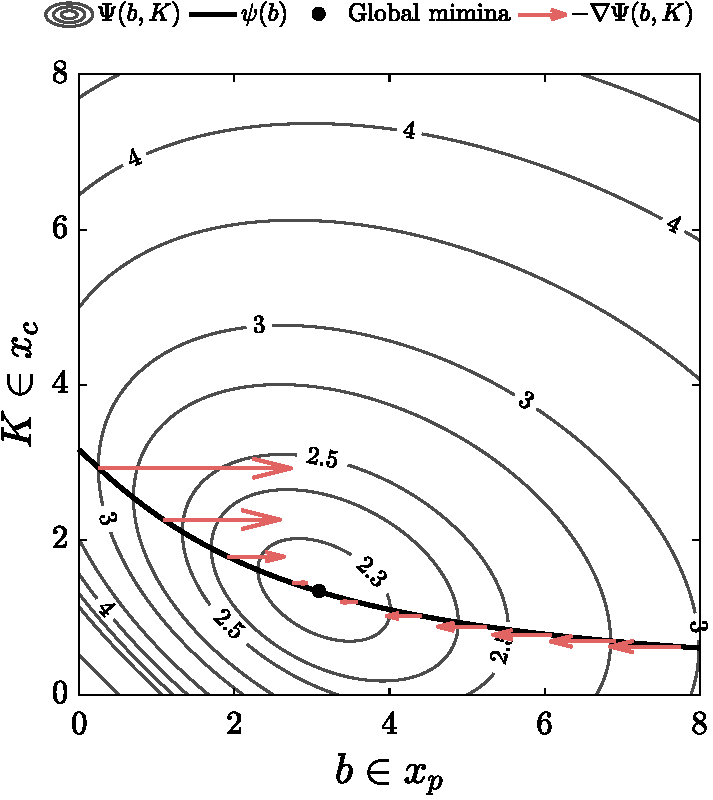
\includegraphics[width=\textwidth]{../ch3/figures/T2_1_PSI}
        \caption{$\Psi(b,K)$.\label{fig:ch3:T2_1_PSI}}
\end{subfigure}% 
\begin{subfigure}[b]{0.266666666667\columnwidth}
       \centering
        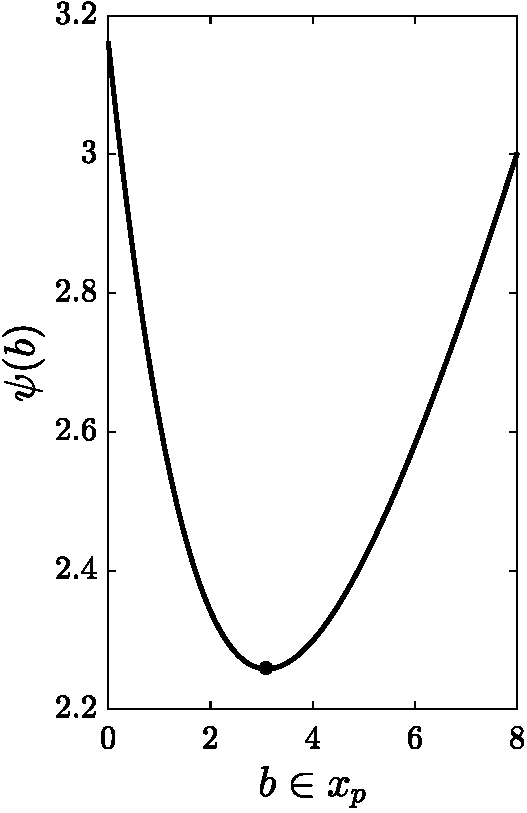
\includegraphics[width=\textwidth]{../ch3/figures/T2_1_nested}%
        \vspace{0.03in}
        \caption{$\psi(b)$.\label{fig:ch3:T2_1_nested}}
\end{subfigure}%
\caption[Scalar plant, scalar control problem (TP1) results]{Scalar plant, scalar control problem (TP1) results with $q=10$, $r=1$, $w_c = 1$, and $w_p = 0.3$.\label{fig:ch3:T2_1}}
\end{figure}


% new paragraph
For this problem, the ARE defined in Eqn.~(\ref{eq:ch3:are}) is a single quadratic equation: $0 = q - 2 b P - P^2/r$. The solution to this equation defines the gains of a full-state feedback optimal control law and therefore can be used to obtain the potential inner-loop optimal control designs, $M(\bxp)$, in a nested formulation. This is visualized in Fig.~\ref{fig:ch3:T2_1_PSI} as the solid black curve. We note that this is a subspace of $\Omega$, or simultaneous feasible set.
Comparing Fig.~\ref{fig:ch3:T2_1_PSI} and Fig.~\ref{fig:ch3:T2_1_nested}, we can visualize directly the difference between $\Psi(\bxp,\bxc)$ and $\psi(\bxp)$. We also note that the gradient of the nested solution trajectory in Fig.~\ref{fig:ch3:T2_1_PSI} is always orthogonal to the $K$-axis since it is the optimal gain value for a given $b$. 

% new paragraph
The coupling between the plant and control design variables is also present, noting the ``tilt'' of the level sets. Therefore, a sequential method would not be guaranteed to arrive at the global optima (but an iterative sequential strategy would in TP1)~\cite{Fathy2001a}.
In TP1, from all starting conditions, both the simultaneous and nested solution strategies arrive at the global optimum.
Although this is an extremely simple co-design problem, it does help visualize a number of important concepts.

%----------------------------
% this is the figures for TP2
\begin{figure*}
\centering

\begin{subfigure}[b]{1\textwidth}
       \centering
        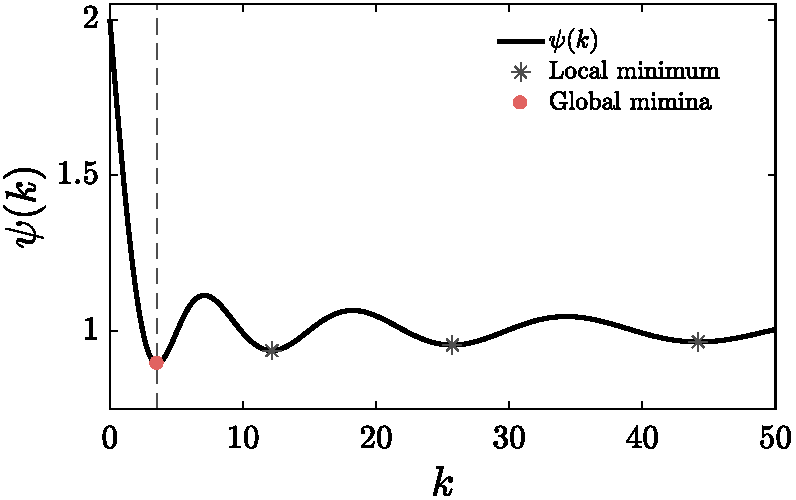
\includegraphics[width=0.333\textwidth]{../ch3/figures/T1_1_PSI}%
        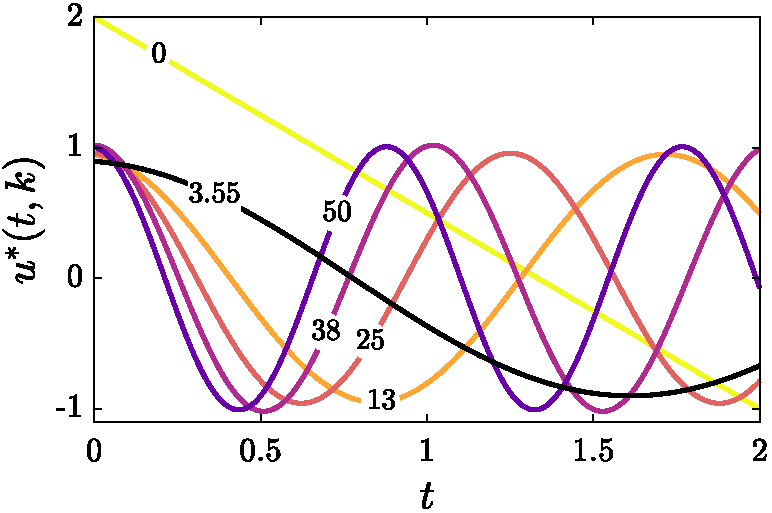
\includegraphics[width=0.333\textwidth]{../ch3/figures/T1_1_U}%
        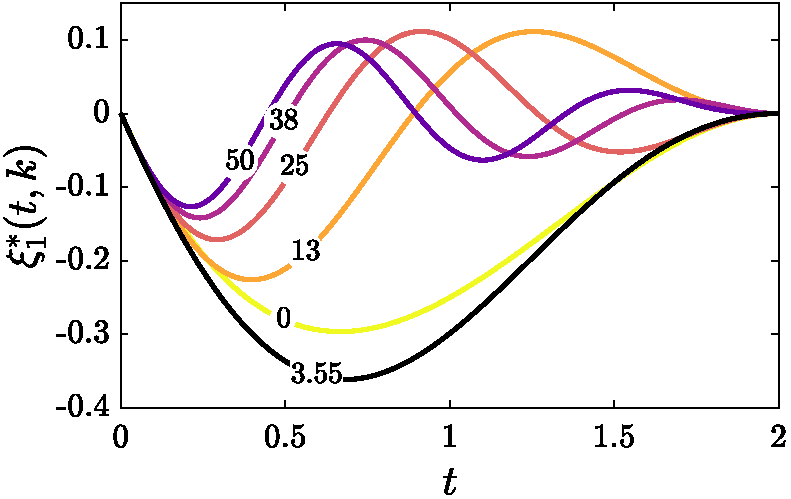
\includegraphics[width=0.333\textwidth]{../ch3/figures/T1_1_X}%
        \caption{TP2 results demonstrating a large number of
local solutions with $t_f = 2$, $x_0 = 0$, and $v_0 = -1$ (different values of $k$ marked).\label{fig:ch3:T1_1}}
\end{subfigure}%

\begin{subfigure}[b]{1\textwidth}
  \centering
  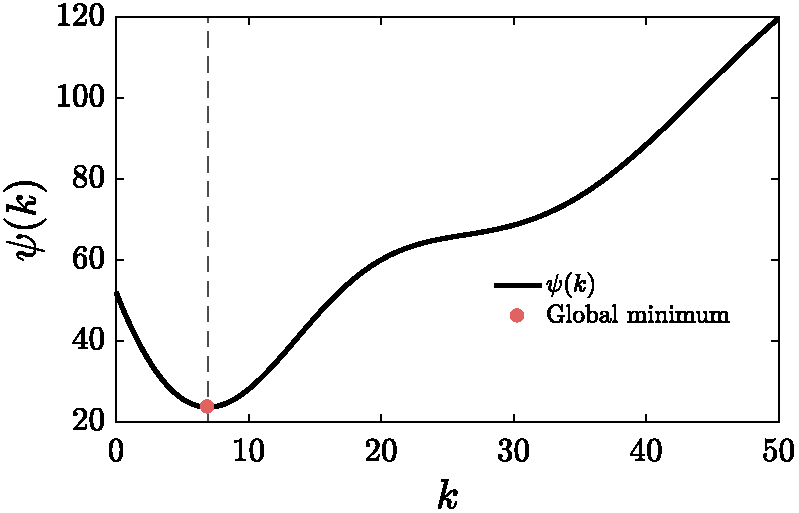
\includegraphics[width=0.333\textwidth]{../ch3/figures/T1_2_PSI}%
  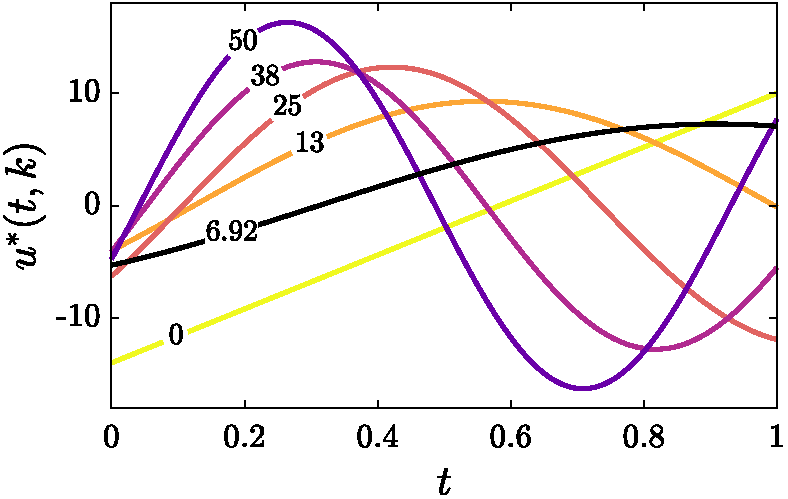
\includegraphics[width=0.333\textwidth]{../ch3/figures/T1_2_U}%
  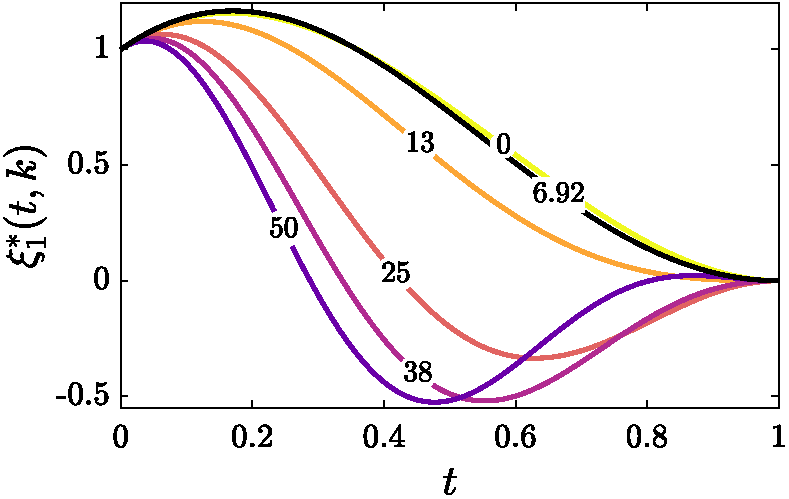
\includegraphics[width=0.333\textwidth]{../ch3/figures/T1_2_X}%
  \caption{TP2 results demonstrating single global minimum with $t_f = 1$, $x_0 = 1$, and $v_0 = 2$ (different values of $k$ marked).\label{fig:ch3:T1_2}}
\end{subfigure}%

\begin{subfigure}[b]{1\textwidth}
  \centering
  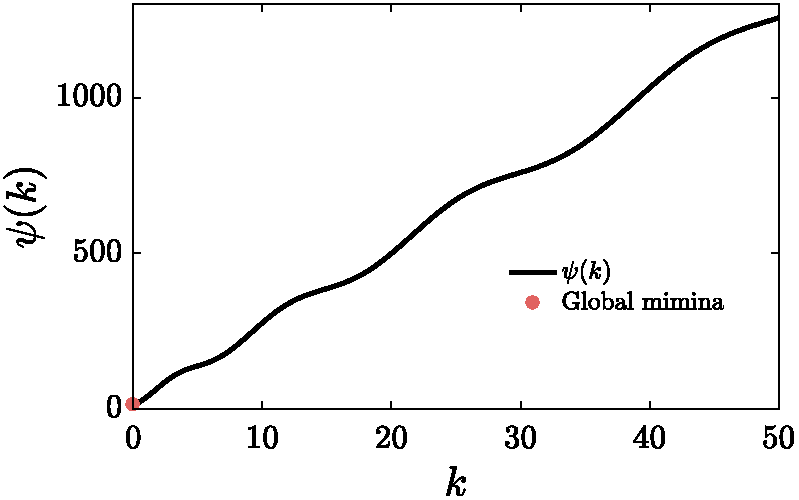
\includegraphics[width=0.333\textwidth]{../ch3/figures/T1_3_PSI}%
  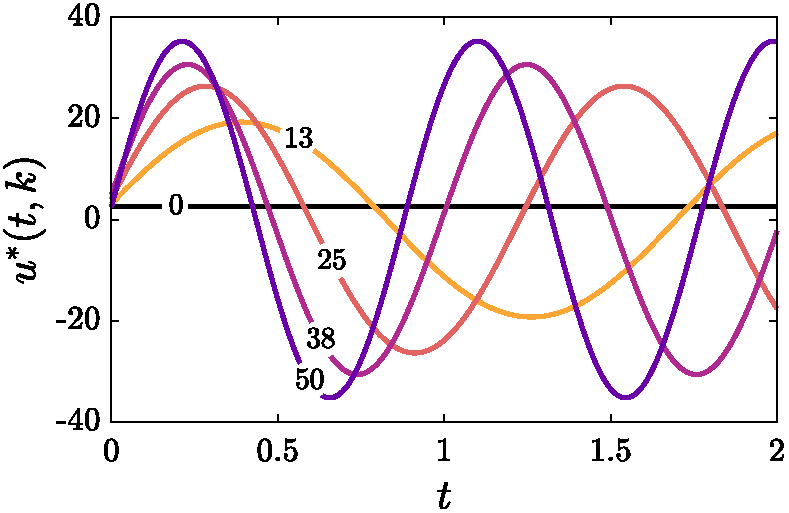
\includegraphics[width=0.333\textwidth]{../ch3/figures/T1_3_U}%
  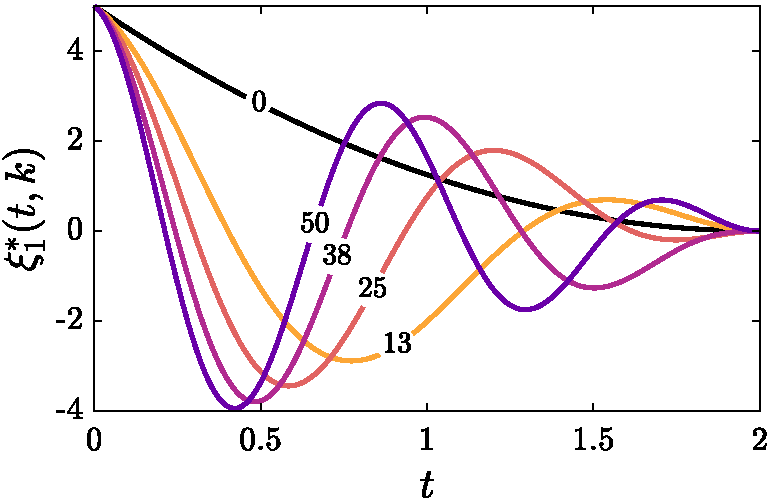
\includegraphics[width=0.333\textwidth]{../ch3/figures/T1_3_X}%
  \caption{TP2 results demonstrating degenerate plant solution with $t_f = 2$, $x_0 = 5$, and $v_0 = -5$ (different values of $k$ marked).\label{fig:ch3:T1_3}}
\end{subfigure}%

\caption[Co-design transfer problem (TP2) results]{Co-design transfer problem (TP2) results for various values of the problem parameters.\label{fig:ch3:T1}}
\end{figure*}% 
% moved here for positioning purposes
%----------------------------

%-----------------------------------------------------------------------------
\subsection{Test Problem 2: Co-Design Transfer \label{sec:ch3:transfer}}

Consider the following simple co-design problem that seeks to move a second-order system from an arbitrary initial state to rest while minimizing control effort:
\begin{subequations}
\begin{align}
\min_{k,u(t)} \quad & \int_{0}^{t_f} u^2 dt \\
\text{subject to:} \quad & \dot{\bxi} = \begin{bmatrix} 0 & 1 \\ -k & 0 \end{bmatrix}\bxi + \begin{bmatrix} 0 \\ 1 \end{bmatrix} u \\
& \textcolor{light-gray}{\phi_1 := }\ \xi_1(0) - x_0 = 0, \ \textcolor{light-gray}{\phi_2 := }\  \xi_2(0) - v_0 = 0 \\
& \textcolor{light-gray}{\phi_3 := }\ \xi_1(t_f) = 0, \ \textcolor{light-gray}{\phi_2 := }\  \xi_2(t_f) = 0
\end{align}
\end{subequations}

\noindent where $k\in \bm{x}_p$ and $u(t) \in \bm{x}_c$.
The solution for $u^*(t,k)$ (i.e.,~the nested strategy) can be obtained by scaling the problem~\cite{Herber2017c} into an equivalent DO problem in Ref.~\cite[pp.~166--167]{Bryson1975a} (details of this procedure are in Sec.~\ref{sec:ch4:transfer}):
\begingroup
\allowdisplaybreaks
\begin{subequations}
\label{eq:ch3:ex2_usol}
\begin{align}
u^*(t,k) &= - \frac{2k}{k t_f^2 - \sin^2(\sqrt{k} t_f)} \left( c_1(t,k) x_0 + c_2(t,k) \frac{v_0}{\sqrt{k}} \right) \\
c_1(t,k)  &= \sin\left( \sqrt{k}(t_f - t) \right)\sin\left(\sqrt{k}t_f\right) - \sqrt{k} t_f \sin \left(\sqrt{k}t \right) \\
c_2(t,k)  &= - \cos\left(\sqrt{k}(t_f-t)\right) \sin\left(\sqrt{k}t_f\right) + \sqrt{k} t_f \cos\left(\sqrt{k}t\right)
\end{align}%
\end{subequations}%
\endgroup

\noindent If $k=0$, then the solution above is not valid and $u^*$ is linear with respect to $t$. The original objective function can now be computed analytically by integrating the square of Eqn.~(\ref{eq:ch3:ex2_usol}). With this closed-form expression for the objective function, an optimality condition for $k$ can be derived using Eqn.~(\ref{eq:ch3:nested_stationarity}).

% new paragraph
The results for this TP are shown in Fig.~\ref{fig:ch3:T1} for various values of the problem parameters.
In Fig.~\ref{fig:ch3:T1_1}, there are a large number of local solutions of $\psi(k)$ and a clear global minimum at $k^*=3.554$.
In Fig.~\ref{fig:ch3:T1_2}, for the different values of the problem parameters, there is a single global minimum at $k^*= 6.924$.
Finally in Fig.~\ref{fig:ch3:T1_3}, there is a global minimum with $k^*=0$, i.e.,~the plant solution is degenerate.

% new paragraph
From these results, it is clear that caution should be used when claiming a global optimal co-design solution is found. Global search algorithms could improve the confidence of finding the true optimal solution such as a multistart approach or genetic algorithms~\cite{Papalambros2017a}. 
The control solution in Eqn.~(\ref{eq:ch3:ex2_usol}) demonstrates the complicated nature of the analytical solutions for even the simplest of co-design problems.
This problem may be a particularly useful TP as it is a well-posed co-design problem with a single system-level objective, general boundary conditions, and a closed-form OLC solution.

%-----------------------------------------------------------------------------
\subsection{Test Problem 3: Simple SASA}

The final TP is a co-design problem that was used directly in a detailed co-design study.
The co-design study focused on developing a novel \glsfoo[noindex]{SASA} system for spacecraft pointing control and jitter reduction~\cite{Chilan2017a} (please see Sec.~\ref{sec:ch4:sasa} for a detailed discussion of the connections to the detailed study in Chapter~\ref{ch:7}). Both the geometric properties of the solar array and OLC voltages along the array were the design variables.
To help provide some insight into the results of the original design study, a much simpler, but still representative, co-design problem was proposed:
\begin{subequations}
\label{eq:ch3:sasa_prob2}
\begin{align}
\min_{k,u(t)} \quad & - \xi_1(t_f) \\
\text{subject to:} \quad & \dot{\bm{\xi}} = \begin{bmatrix} 0 & 1 \\ -k/J & 0 \end{bmatrix} \bm{\xi} + \begin{bmatrix} 0 \\ 1/J \end{bmatrix} u \\
& \textcolor{light-gray}{\phi_1 := }\ \xi_1(0) = 0, \quad \textcolor{light-gray}{\phi_2 := }\  \xi_2(0) = 0 \\
& \textcolor{light-gray}{\phi_3 := }\  \xi_2(t_f) = 0 \\ 
& \textcolor{light-gray}{C_1 := }\  u - u_{\max} \leq 0, \quad \textcolor{light-gray}{C_2 := }\ -u - u_{\max} \leq 0
\end{align}
\end{subequations}

\begin{figure*}[t]
\centering
\begin{subfigure}[b]{0.333\textwidth}
       \centering
        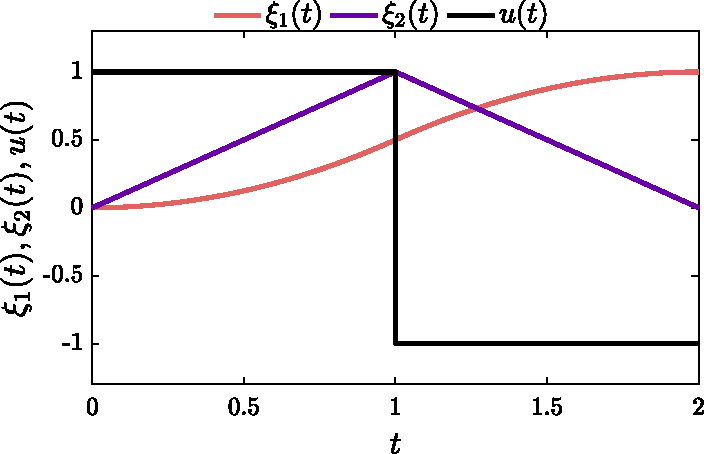
\includegraphics[width=\textwidth]{../ch3/figures/sasa_1.pdf}
        \caption{$k=0$.\label{fig:ch3:sasa_1}}
\end{subfigure}% 
\begin{subfigure}[b]{0.333\textwidth}
       \centering
        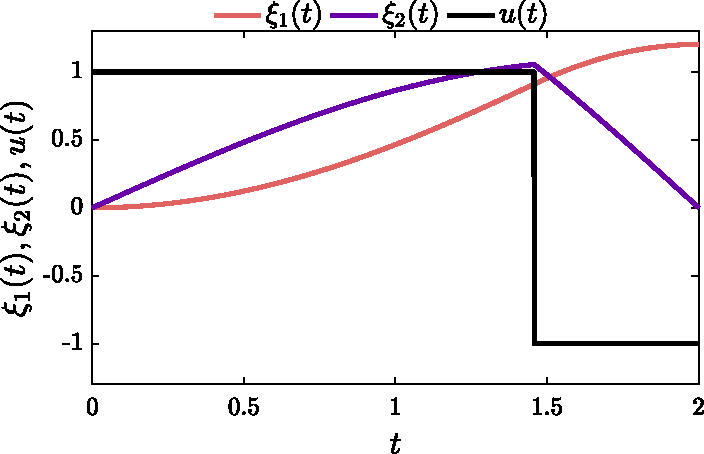
\includegraphics[width=\textwidth]{../ch3/figures/sasa_2.pdf}
        \caption{$k^*=0.8547$.\label{fig:ch3:sasa_2}}
\end{subfigure}%
\begin{subfigure}[b]{0.333\textwidth}
       \centering
        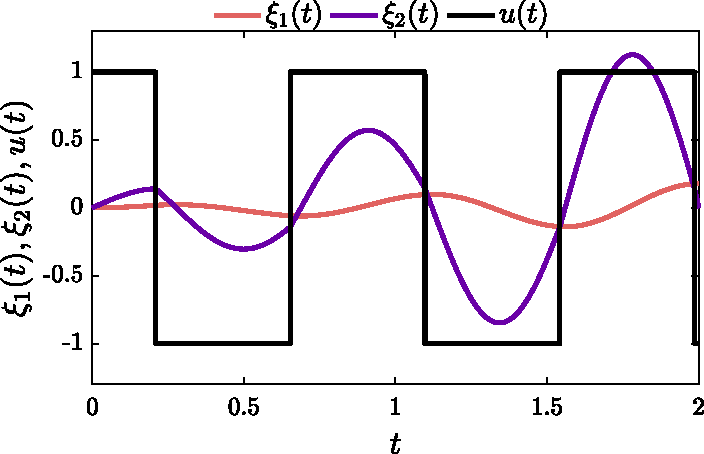
\includegraphics[width=\textwidth]{../ch3/figures/sasa_3.pdf}
        \caption{$k=50$.\label{fig:ch3:sasa_3}}
\end{subfigure}%
\caption[Simple SASA test problem (TP3) results]{Simple SASA test problem (TP3) results with $J=1$, $t_f=2$, and $u_{\max}=1$.\label{fig:ch3:sasa}}
\end{figure*}

\noindent where $k \in \bm{x}_p$  and $u(t) \in \bm{x}_c$. The results for this problem are shown in Fig.~\ref{fig:ch3:sasa} for various values of $k$ including $k^* = 0.8547$.

The OLC exhibits bang-bang behavior~\cite{Bryson1975a, Liberzon2012a}, i.e.,~$u$ is at either the minimum or maximum value. 
Using the control stationarity condition in Eqn.~(\ref{eq:ch3:ocsd_cond_2}), we can show directly that the Hamiltonian is minimized if $u$ exhibits bang-bang behavior, but determining the locations of the switching is quite challenging.
In a nested strategy, the number and location of the switches vary for different values of $k$ (see Fig.~\ref{fig:ch3:sasa_3} containing five switches while the optimal co-design solution only contains one switch in Fig.~\ref{fig:ch3:sasa_2}). This is a direct example of the discussion in Sec.~\ref{sec:ch3:approx} motivating the using of DT in co-design (see Sec.~\ref{sec:ch3:dt}).
The nested co-design solutions were found using DT formulated as a QP with both the composite quadrature and defect constraints based on the trapezoidal rule~\cite{Biegler2010a, Betts2010a, Herber2014a}.

% new paragraph
TP3 is an attractive TP as the closed-form solution for the simultaneous strategy can be computed to a high degree of accuracy, and it exhibits challenging behavior associated with inequality path constraints.

%---------------------------------------------------------------------
\section{Summary \label{sec:ch3:conclusion}}

In this chapter, general combined plant and controller design (or co-design) problems were examined.
A large portion of existing co-design theory has focused on specific DO formulations, leaving many open questions for co-design studies that do not fit the previous definitions. 

% new paragraph
There are two basic co-design solution strategies: simultaneous and nested.
The problem formulations for both strategies wer{}e presented and a discussion of the formulation elements was provided.
The nested strategy was presented as two-level optimization problem including a characterization of the differences in the feasibility region between the two strategies.
This motivated the outer-loop feasibility constraint as one approach for ensuring that for every candidate plant design, the control subproblem is well-posed.

% new paragraph
The natural next step was the presentation of the optimality conditions for both methods.
For the simultaneous strategy, the optimality conditions were derived using only Pontryagin's minimum principle and an augmented state vector.
Due to a number of challenges associated with the optimality conditions, practical solution considerations were discussed with a focus the motivating reasons for using DT in co-design (e.g.,~the activity of inequality path constraints).
Finally, three test problems were presented.
These problems were fairly simple but highlighted a number of key concepts including coupling, the difference between the feasible regions for each strategy, general boundary conditions, inequality path constraints, system-level objectives, and complexity of the closed-form solutions.

% new paragraph
This chapter seeks to provide a foundation for additional advances in general co-design theory. 
The outer-loop feasibility constraint warrants further investigation. 
Better comparisons between the two strategies are needed, especially for co-design problems without a specific form of the inner loop.
Developing methods for reducing total computational expense is also an important area such as the suggestion in Ref.~\cite{Kelly2015a} for treating plant variables like dummy states (or control) or alternative general strategies such decentralized optimization \cite{Allison2010b, Liu2017a}.
Finally, development of test problems that are more realistic could help answer some of the open questions. % co-design
\mychapterfoot{Scaling of Dynamic Optimization Formulations\label{ch:4}}

\footnotetext{Elements of this chapter are based on work completed in Ref.~\cite{Herber2017c}.}

%--- epigraph
\epigraph{\textit{``Behind complexity, there is always simplicity to be revealed. \\
Inside simplicity, there is always complexity to be discovered.''}}{\textmd{G. Yu} \cite{Yu2004a}}

\section{Introduction\label{sec:ch4:introduction}}

Dynamics play an increasingly important role in the advancement of many complex engineering systems \cite{Allison2014a}.
The primary goal of design studies is to find solutions and gain a general understanding of the design trade-offs, building design knowledge for the particular system.
Here we show how scaling can facilitate finding accurate, generalizable, and intuitive information for the design problem at hand.

% new paragraph
At a basic level, scaling is simply the stretching, squeezing, and shifting of the problem elements and this can include the time continuum, design variables, constraints, objective function, etc.
For example, if we have the inequality constraint $a x \leq b$ and $b > 0$, then we can arrive at an equivalent scaled constraint $\rho x \leq 1$ where $\rho=a/b$.
The mechanics of scaling are fairly straightforward but proper utilization of scaling is heavily reliant on the creativity and intuition of the designer \cite{Holmes2009a}. 
This barrier may be one of the reasons why scaling is often overlooked, but these manipulations can help define problem formulations that are 1) better suited for analysis and 2) more favorable for solution methods (e.g.,~higher quality solutions and faster convergence). 
In this chapter, we provide the necessary theory to scale \glsfoo[noindex]{DO} problems and some examples of how to use scaling in the context of a design study.

% new paragraph
First, we review some of the previous uses of scaling focusing on examples relevant to obtaining solutions and the analysis of engineering design problems.
Some of these examples are quite well-established, while others are rarely used. 
The context that all the examples provide is crucial for defining the most useful scaling procedure for a particular design problem.
Some authors state that the importance of scaling can only be fully appreciated through examples \cite{Groesen2007a}.

\subsection{Previous Uses of Scaling \label{sec:ch4:uses}}

% new paragraph
One of the primary uses of scaling is to reduce the number of parameters in a set of equations \cite{Cengel2006a, Groesen2007a,Holmes2009a}.
Under certain conditions, algebraic manipulations can lead to a reduced set of parameters (e.g.,~consider the example above where now $\rho$ is the only parameter).
Buckingham's Pi theorem is one well-known method for reducing the number of parameters, which applies constraints on the mathematical interaction of the fundamental units of the system and does not necessarily need a specific mathematical expression of the system (e.g.,~the equations of motion) \cite{Buckingham1914a, Holmes2009a, Groesen2007a}.
However, this approach does not necessarily leverage the equations of motion nor does it directly consider the numerical aspects of finding approximate solutions to the system of equations. 

% new paragraph
Another common use for scaling is to determine characteristic properties of the system. These properties may be scalars or functions. Characteristic scalars are well studied in many engineering domains such as fluid dynamics and heat transfer \cite{Cengel2006a}. An example of such a scalar is the Reynolds number, a dimensionless constant that relates inertial forces to viscous forces within a fluid \cite{Cengel2006a}. Other examples include intrinsic resonance frequency, length, damping, or time constant.  Such characteristic properties can be conceptually easier to understand \cite{Holmes2009a}.
These properties may be well understood for classical domains but for others, these characteristic properties may be the key to building the required knowledge of the system.

% new paragraph
In dynamic or spatially-defined systems, it can be advantageous to scale entire continuous functions. For example, for an initial value problem, characteristic solutions to the differential equation can be obtained that scale linearly with the initial condition \cite{Holmes2009a}. Under certain conditions, even the solution to optimization problems can be scaled for different parameter values. There are some potentially restrictive issues with directly scaling optimal solutions that are discussed in Ref.~\cite{Kittirungsi2008a}. 

% new paragraph
The central tool in many design studies is design optimization.
Frequently, the solution of a single optimization problem is not sufficient to address the complicated nature of a design activity.
This typically leads to variations on the problem formulation elements (e.g.,~parametric sweeps of the problem's parameters).
Both reducing the number of parameters and obtaining scalable solutions can greatly improve this process.

% new paragraph
Scaling can also be used to help decide if certain parts of a model or optimization formulation are small, and therefore negligible in a consistent manner \cite{Holmes2009a, Khalil2002a}.
This can help with developing asymptotic solutions to differential equations, reveal multiple-time-scale structures, and simplify simulations, stability analysis, and controller design \cite{Khalil2002a}.
With respect to optimization formulations, scaled forms of the constraints can help determine if certain constraints are likely to be active or inactive based on the magnitude of their scaled forms \cite{Papalambros2017a}.

% new paragraph
One common motivation for scaling in optimization is to change the order of magnitude of the variables and constraints to be more favorable for computation \cite{Papalambros2017a, Rao2010a}.
Large order of magnitude differences in either the variables or function values can produce ill-conditioned matrices such as Jacobians and Hessians; thus, algorithmic calculations may become unstable or inefficient \cite{Papalambros2017a}.
Systematic preconditioning methods have been developed to scale special cases of problem elements such as linear constraints \cite{Bergamaschi2004a, Benzi2002a}.
This has been observed to be especially important in DO to ensure robustness and accuracy \cite{Rao2010a, Betts2010a}.
Some automatic scaling procedures have been developed to help alleviate some of the computational issues associated with solving dynamic optimization problems \cite{Rao2010a}.

% new paragraph
Scaling has also been directly included in some design studies.
In Ref.~\cite{Kittirungsi2008a}, the author develops a method for assessing the importance of scaling laws in design optimization and approximate similitude metrics for obtaining dynamically similar optimal solutions. There have been a number of interesting examples of controller design that utilizes scaling, including Refs.~\cite{Ghanekar1997a, Brennan2001a}, but are typically limited to linear feedback controllers. 
Additionally, in Ref.~\cite{Chilan2017a}, the authors utilized scaling to understand the trends found in the solutions to a more complete optimization formulation (and this example will be discussed in detail in Sec.~\ref{sec:ch4:sasa}).

% new paragraph
Some final uses include performing scaled tests \cite{Cengel2006a, Holmes2009a} and checking for dimensional homogeneity \cite{Cengel2006a}.
All of the examples provide a rich history of scaling in engineering activities.

%----------------------------------------------------------------------
\subsection{Dynamic Optimization \label{sec:ch4:do}}

In this chapter, we consider design optimization problems that are well-posed as the following DO problem:
\begin{subequations}
\label{eq:ch4:sim_prob}
\begin{align}
\min_{\bu, \bp} \quad & \int_{t_0}^{t_f} \lagrange \left( t, \bxi, \bu, \bp \right) dt \ + \mayer \left( \bxi(t_0), \bxi(t_f), \bu, \bp \right) \label{eq:ch4:sim_obj} \\
\text{subject to:} \quad & \dot{\bxi \glsfoo[noindex]{timederiv}} - \glsname{f} \left( t, \bxi, \bu, \bp \right) = \bzero \label{eq:ch4:simcodesign_dyn} \\
& \gls{path} \left( t, \bxi, \bu, \bp \right) \leq \bzero \label{eq:ch4:sim_path} \\
& \gls{boundary} \left( \bxi(t_0), \bxi(t_f), \bp \right) \leq \bzero \label{eq:ch4:sim_bound}
\end{align}
\end{subequations}

\noindent where the optimization variables are \gls{parameters} (time-independent variables) and \gls{olc} (open-loop control variables), \gls{time} is the time continuum defined between $t_{\glsfoo[noindex]{initial}}$ and $t_{\glsfoo[noindex]{final}}$, and \gls{states} are the states. 
The objective function in Eqn.~(\ref{eq:ch4:sim_obj}) is in Bolza form where \gls{lagrange} is the Lagrange (running cost) term and \gls{mayer} is the Mayer (terminal cost) term.
Equation~(\ref{eq:ch4:simcodesign_dyn}) enforces the dynamics modeled as a first-order \glsfirst{ODE}, Eqn.~(\ref{eq:ch4:sim_path}) enforces any time-varying path constraints, and Eqn.~(\ref{eq:ch4:sim_bound}) enforces any time-independent constraints. 

% new paragraph
There are two approaches for finding solutions to Prob.~(\ref{eq:ch4:sim_prob}).
Indirect methods utilize the optimality conditions of the infinite-dimensional DO problem \cite{Bryson1975a, Biegler2010a, Betts2010a}.
It can be quite challenging (or impossible) to solve these equations analytically. 
Therefore, numerical methods are often employed that provide approximate solutions to the original problem.
The alternative solution methods are known as direct methods \cite{Biegler2010a, Betts2010a}. Instead of stating the optimality conditions, the control and/or state are parametrized using function approximation and the objective function is approximated using numerical quadrature.
This creates a discrete, finite-dimensional problem that then is optimized using large-scale \glsfoo[noindex]{NLP} solvers \cite{Biegler2010a, Betts2010a, Herber2014a, Rao2010a}.
Scaling can be advantageousness for both methods.

% new paragraph
The optimality conditions will be important when scaling DO formulations and are the same optimality conditions for the simultaneous co-design method in Eqn.~(\ref{eq:ch3:opt_cond_sim}).

\section{Theory of Scaling Dynamic Optimization Formulations\label{sec:ch4:theory}}

Now the theory of scaling DO formulations is presented with examples to help illustrate the concepts.
The basics are described first, which are applicable to sets of \glsfoo[noindex]{DAE}.
Second is scaling in the context of optimization formulations.

%----------------------------------------------------------------------
\subsection{Scaling Basics \label{sec:ch4:basics}}

The first step when scaling a set of equations is to introduce a change of variables. Here we consider linear scaling with:
\begin{subequations}
\label{eq:ch4:scale}
\begin{align}
x &= \alpha_x \mybar{x} + \beta_x \\
y(x) &= \alpha_y \mybar{y}(x) + \beta_y
\end{align}
\end{subequations}

\noindent where \gls{xind} is an independent variable, \gls{ydep} is a dependent variable, $\{ \mybar{x\glsfirst{scale}}, \mybar{y} \}$ are the new dimensionless variables, and $\{ \gls{alpha}_x, \gls{beta}_x, \alpha_y, \beta_y \}$ are the user-defined scaling constants. The only restriction on the scaling constants is $\alpha \neq 0$ to avoid an ill-defined mapping between the scaled and original variables. Other types of scaling are possible \cite{Boyd2009a} but the linear scaling rule often proves to be suitable for DO.

To substitute higher-order derivatives properly, we need to consider the chain rule and linearity of differentiation \cite{Strang1991a}:
\begin{align}
\label{eq:ch4:derivative}
\frac{d^n y}{d x^n} = \frac{\alpha_y}{\alpha_x^n} \frac{d^n \mybar{y}}{d \mybar{x}^n}
\end{align}

\noindent where $n$ is the order of the derivative. If integrals are present, we can use integration by substitution when changing the integral limits \cite{Strang1991a}:
\begin{align}
\label{eq:ch4:integral}
\int_{x_0}^{x_f} f(x) dx = \alpha_x \int_{\bar{x}_0}^{\bar{x}_f} f(\alpha_x \mybar{x} + \beta_x) d\bar{x}
\end{align}

\noindent where $f(x)$ is some function and the integration limits have been shifted from $\{x_0,x_f\}$ to $\{\bar{x}_0,\bar{x}_f\}$. With this small set of formulas, we can apply scaling to all the problem elements of Prob.~(\ref{eq:ch4:sim_prob}).

% new paragraph
The original system of DAEs can have problem parameters, denoted \gls{rho}.
Through suitable choices of scaling variables, every system of DAEs with dimensional homogeneity (i.e.,~the dimensions on the left and right sides are the same) can be transformed into a dimensionless set of DAEs \cite{Holmes2009a}.
This will lead to the creation of dimensionless parameters, denoted $\bar{\bm{\rho}}$, and will prove quite important as they are critical to many of the uses discussed in Sec.~\ref{sec:ch4:uses}. 
These dimensionless quantities can be the same as the dimensionless quantities derived by using Buckingham's Pi theorem \cite{Buckingham1914a, Holmes2009a, Groesen2007a}.
Here we assume that all equations, inequalities, and inequations have dimensional homogeneity.

%----------------------------------------------------------------------
\subsubsection{Example: Spring-Mass System \label{sec:ch4:ex_mass_spring}}

To illustrate the concepts of the previous section, we apply scaling to a simple spring-mass system.
The first step is to write down the equations and assumptions:
\begin{subequations}
\begin{gather}
m \ddot{y}(t) + k y(t) = 0 \\
y(t_0) = y_0, \quad \dot{y}(t_0) = v_0 \\
m, k > 0, \quad y_0 \neq 0
\end{gather}
\end{subequations}

\noindent In this system, the independent variable is $t$ and the dependent variable is $y$.
Now consider the following change of variables based on simple scaling in Eqn.~(\ref{eq:ch4:scale}):
\begin{gather}
t = \alpha_t \bar{t} + \beta_t, \quad y(t) = \alpha_y \mybar{y}(t) 
\end{gather}

\noindent The higher-order derivatives, using Eqn.~(\ref{eq:ch4:derivative}), are then:
\begin{align}
\frac{dy(t)}{dt} = \frac{\alpha_y}{\alpha_t} \frac{d\mybar{y}(\mybar{t})}{d\mybar{t}}, \quad \frac{d^2y(t)}{dt^2} = \frac{\alpha_y}{\alpha_t^2} \frac{d^2\mybar{y}(\mybar{t})}{d\mybar{t}^2}
\end{align}

We are free to choose the scaling constants so let's first look at the system of DAEs with the substitutions applied:
\begin{subequations}
\begin{gather}
m \frac{\alpha_y}{\alpha_t^2} \frac{d^2\mybar{y}(\mybar{t})}{d\mybar{t}^2} + k \alpha_y \mybar{y}(\mybar{t}) = 0 \\
\alpha_y \mybar{y}\left( \frac{t_0-\beta_t}{\alpha_t} \right) = y_0, \quad \frac{\alpha_y}{c_t} \frac{d \mybar{y}}{d\mybar{t}}\left( \frac{t_0-\beta_t}{\alpha_t} \right) = v_0
\end{gather} 
\end{subequations}

\noindent We can perform some algebraic manipulations to make the left-hand side of the equations have unity coefficients:
\begin{subequations}
\begin{gather}
\frac{d^2\mybar{y}(\mybar{t})}{d\mybar{t}^2} = - \frac{k \alpha_t^2}{m} \mybar{y}(\mybar{t}) \\
\mybar{y}\left( \frac{t_0-\beta_t}{\alpha_t} \right) = \frac{y_0}{\alpha_y}, \quad \frac{d \mybar{y}}{d\mybar{t}}\left( \frac{t_0-\beta_t}{\alpha_t} \right) = \frac{\alpha_t v_0}{\alpha_y}
\end{gather} 
\end{subequations}

\noindent Now, consider the following choice of the scaling constants:
\begin{align}
\alpha_t = \sqrt{\frac{m}{k}}, \quad \beta_t = t_0,\quad \alpha_y = y_0
\end{align}

\noindent Then the scaled system of DAEs is:
\begingroup
\allowdisplaybreaks
\begin{subequations}
\begin{gather}
\frac{d^2\mybar{y}(\mybar{t})}{d\mybar{t}^2} = - \mybar{y}(\mybar{t}) \\
\mybar{y}\left( 0 \right) = 1, \quad \frac{d \mybar{y}}{d\mybar{t}}\left( 0 \right) = \frac{v_0}{y_0} \sqrt{\frac{m}{k}} := \bar{\rho}_1
\end{gather} 
\end{subequations}%
\endgroup

\noindent We see that this choice of constants results in a differential equation with unity coefficients.
The original system had five parameters, but this scaled system now has only one, denoted $\bar{\rho}_1$, and is dimensionless.
Furthermore, the initial position does not depend on any parameters. The scaling constant $\alpha_t= \sqrt{m/k}$ is typically referred to as the characteristic time constant for this system (also known as the reciprocal of the natural frequency).

\begin{figure}[t]
\centering
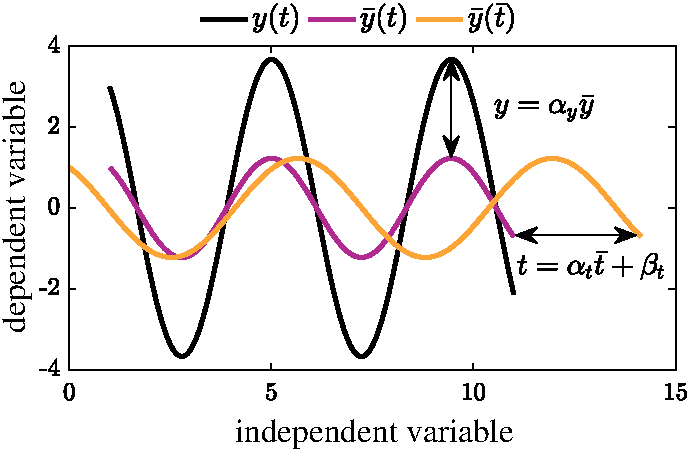
\includegraphics[width=0.5\columnwidth]{../ch4/figures/scaling_example}
\caption[Spring-mass system]{Spring-mass system with parameter values $k = 4$, $m = 2$, $y_0 = 3$, $v_0 = -3$, $t_0 = 1$, and $t_f = 11$. \label{fig:ch4:scaling_example}}
\end{figure}

Both the scaled and original solutions to this initial value problem are shown in Fig.~\ref{fig:ch4:scaling_example}.
We see the stretching, squeezing, and shifting of the trajectory based on the scaling rules.
The scaled trajectory might be more favorable to numerical approximation methods since the average magnitude of its derivative is closer to unity and consistent across the range of parameter values.

\subsection{Scaling Dynamic Optimization Problems \label{sec:ch4:scaled_opt}}

We first denote the original problem formulation as \gls{Pformulation} with optimality conditions \gls{O} and optimal solution $\gls{x}^{\glsfoo[noindex]{optimal}}$.
Now the scaled formulation is denoted $\bar{P}$ with optimality conditions $\bar{O}$ and optimal solution $\bar{\bm{x}}^*$.
For each problem, there may be problem parameters each denoted $\bm{\rho}$ and $\bar{\bm{\rho}}$, respectively.
The optimization variables are related with the scaling function \glsfirst{S}: $\bm{x} = S(\bar{\bm{x}}, \bm{\rho})$ where for each optimization variable, a linear scaling law defined in Eqn.~(\ref{eq:ch4:scale}) exists that may depend on the problem parameters.
Now for a given value of $\bm{\rho}$, the optimal solution to the two problems are clearly equivalent: if $\bm{x}^*$ solves $P$, then $\bar{\bm{x}}^* = S^{-1}(\bm{x}^*, \bm{\rho})$ solves $\bar{P}$; if $\bar{\bm{x}}^*$ solves $\bar{P}$, then $\bm{x}^* = S(\bar{\bm{x}}^*, \bm{\rho})$ solves $P$ \cite{Boyd2009a}.

% new paragraph
In some design studies, finding the optimal solution with respect to a single set of parameter values is sufficient to complete the design task.
However, many require solutions that vary with respect to the parameters, i.e.,~$\bm{x}^*(\bm{\rho})$ for various values of $\bm{\rho}$.
We can utilize the scaled problem in this task.
If we are given two sets of parameters, $\bm{\rho}_1$ and $\bm{\rho}_2$, such that $\bar{\bm{\rho}}_1 = \bar{\bm{\rho}}_2$, then we can determine the optimal solution with respect to $\bm{\rho}_2$ utilizing the solution found with $\bm{\rho}_1$:
\begin{align}
\label{eq:ch4:opt_scale}
\bm{x}^*(\bm{\rho}_2) = S ( \bar{\bm{x}}^*( \bar{\bm{\rho}}_1 ), \bm{\rho}_2 )
\end{align}

\noindent The condition that $\bar{\bm{\rho}}_1 = \bar{\bm{\rho}}_2$ is potentially restrictive \cite{Kittirungsi2008a}, but it also can be quite useful.
This implies that we only need to generate solutions for all relevant values of $\bar{\bm{\rho}}$ rather than $\bm{\rho}$, which is favorable since typically $\bar{\bm{\rho}}$ contains fewer elements that the original $\bm{\rho}$.

% new paragraph
Additional scaling might be possible depending on what can be discerned from the activity of the inequality constraints \cite{Papalambros2017a} but will be problem dependent.
If certain constraints are found to be inactive for particular ranges of the problem parameters and the reduced form of the original optimization problem eliminates any dependence on a particular parameter, then solutions may be scaled irrespective of that parameter (as long as the inactivity holds in the original problem).
In DO, there may be infinite-dimensional path constraints where determining the activity can be challenging (one of the primary motivations for direct methods \cite{Herber2017b}). This may lead to solutions that are widely different for minor changes in the problem parameters, so scaling must be done carefully (this is shown in the example in Sec.~\ref{sec:ch4:sasa}).

% new paragraph
To determine how the optimality conditions are related between the original and scaled problems, additional scaling constants for the multipliers need to be introduced.
Then the correct values for these scaling constants must be determined such that a map is known between $O$ and $\bar{O}$.

% new paragraph
The relationships between the optimization formulations, optimality conditions, and optimal solutions for both the original and scaled problems are shown in Fig.~\ref{fig:ch4:map}.
These relations will be discussed in the context of different paths that may be taken to obtain solutions to a particular DO problem.
Consider first the standard case where the original problem is proposed and then an optimal solution is found (e.g.,~using \glsfoo[noindex]{DT} and an NLP solver):
\begin{align*}
P \to \bm{x}^*
\end{align*}

\noindent An alternative is to utilize the optimality conditions in Eqn.~(\ref{eq:ch3:opt_cond_sim}) to obtain an analytical solution or using a numeric indirect method:
\begin{align*}
P \to O \to \bm{x}^*
\end{align*}

Now using scaling, we could instead transform to $P$ to $\bar{P}$, and solve the scaled problem. Then the scaled solution can be mapped back to obtain the original problem's solution:
\begin{align*}
P \to \mybar{P} \to \bar{\bm{x}}^* \to \bm{x}^*
\end{align*}

\noindent The key here is that $\bar{\bm{x}}^*$ can be used to generate multiple $\bm{x}^*$ using Eqn.~(\ref{eq:ch4:opt_scale}). One final approach that may yield the most information from the scaling procedure is utilizing the optimality conditions:
\begin{align*}
P \to O \to \mybar{O} \to \mybar{P} \to \bar{\bm{x}}^* \to \bm{x}^*
\end{align*}

\noindent With this approach, all of the suggestions in this section can be explored such as constraint activity.

\begin{figure}[t]
\centering

\includegraphics[width=0.2\columnwidth]{../ch4/figures/map}
\caption[Relationships between the original and scaled problems]{Relationships between the optimization formulations, optimality conditions, and optimal solutions for both the original and scaled problems. \label{fig:ch4:map}}
\end{figure}

% new paragraph
The following section will use the theory in this section to illustrate scaling in DO with some motivating examples.

%----------------------------------------------------------------
\section{Motivating Examples}
In this section, a number of examples of scaling in DO are presented. Some examples have direct application to existing design problems while others provide a more conceptual illustration. The examples in this section and the many uses described in Sec.~\ref{sec:ch4:uses} provide a strong foundation for using scaling in novel DO design problems. 

\subsection{Example 1: Simple SASA Problem\label{sec:ch4:sasa}}

This first example was developed to better understand the observed trends from an existing design study (for full details see Chapter~\ref{ch:7}).
The co-design study focused on developing a novel \glsfoo[noindex]{SASA} system for spacecraft pointing control and jitter reduction \cite{Chilan2017a}.
In this system, distributed piezoelectric actuators were used to strain the solar arrays, causing reactive forces that could be used to control the bus (spacecraft body) with higher precision, higher bandwidth, and reduced vibrations.

% new paragraph
The observed trend was an optimal constant ratio between the natural period of the first mode, \gls{firstperiod}, and time allotted for performing the maneuver, $t_f$ (which is visualized in Fig.~10 of Ref.~\cite{Chilan2017a}).
There was much discussion on why this ratio seemed to be constant and if there was any significance to the value of this optimal ratio (approximately $T_1/t_f = 4.41$).
To help provide some insight into these questions, a much simpler, but still representative, design problem was proposed.
In Fig.~\ref{fig:ch4:sasa_schematic}, both the original and simplified SASA systems are visualized. The simplified system modeled many of the fundamental phenomena present in the original high-fidelity system using a small number of lumped parameters.

\begin{figure}[t]
\centering
\includegraphics[width=0.6\textwidth]{../ch4/figures/sasa_schematic}
\caption[Illustrations of original and simplified strain-actuated solar array systems]{Illustrations of original and simplified strain-actuated solar array systems in Sec.~\ref{sec:ch4:sasa}. \label{fig:ch4:sasa_schematic}}
\end{figure}

The problem formulation for the simplified system is:
\begin{subequations}
\label{eq:ch4:sasa_prob_1}
\begin{align}
\min_{k,u(t)} \quad & - \theta(t_f) \\
\text{subject to:} \quad & J\ddot{\theta}(t) + k \theta(t) = u(t) \label{eq:ch4:diff_eq} \\
& \theta(0) = \dot{\theta}(0) = 0 \\
& \dot{\theta}(t_f) = 0 \\
& \abs{u(t)} \leq u_{\max}
\end{align}
\end{subequations}

\noindent where \gls{angle} is the relative displacement of the bus, $J$ is related to the inertia ratio between the solar arrays and bus, $u$ is an open-loop control moment applied to the solar array and is bounded by $u_{\glsfirst{max}}$, and \gls{spring} is the stiffness in the solar array.
The boundary constraints enforce the system to start at rest with zero energy and end at rest.
The optimization variables are both $k$ and $u(t)$.
Scaling can be applied to help analyze this DO problem.

\subsubsection{Standard Form}

First, we write the original DO problem in Eqn.~(\ref{eq:ch4:sasa_prob_1}) the standard form:
\begin{subequations}
\label{eq:ch4:sasa_prob_2}
\begin{align}
\min_{k,u(t)} \quad & - \xi_1(t_f) \\
\text{subject to:} \quad & \dot{\bm{\xi}} = \begin{bmatrix} 0 & 1 \\ -k/J & 0 \end{bmatrix} \bm{\xi} + \begin{bmatrix} 0 \\ 1/J \end{bmatrix} u \\
& \textcolor{light-gray}{\phi_1 := }\ \xi_1(0) = 0, \quad \textcolor{light-gray}{\phi_2 := }\  \xi_2(0) = 0 \\
& \textcolor{light-gray}{\phi_3 := }\  \xi_2(t_f) = 0 \\ 
& \textcolor{light-gray}{C_1 := }\  u - u_{\max} \leq 0, \quad \textcolor{light-gray}{C_2 := }\ -u - u_{\max} \leq 0 \\
\text{where:} \quad & \xi_1 = \theta, \quad \xi_2 = \dot{\theta}
\end{align}
\end{subequations}

\noindent The Hamiltonian is then:
\begin{align}
H = \lambda_1 \xi_2 + \lambda_2 \left( -\frac{k}{J} \xi_1 + \frac{u}{J} \right) + \mu_1 \left( u - u_{\max} \right) + \mu_2 \left( -u - u_{\max} \right)
\end{align}

\noindent Now using the conditions in Eqn.~(\ref{eq:ch3:opt_cond_sim}), the additional conditions for optimality are:
\begingroup
\allowdisplaybreaks
\begin{subequations}
\label{eq:ch4:sasa_cond_1}
\begin{gather}
\dot{\lambda}_1 = \frac{k}{J} \lambda_2, \quad \dot{\lambda}_2 = -\lambda_1  \\
0 = \frac{\lambda_2}{J} + \mu_1 - \mu_2 \\
0 = {\mu}_1 \left( u - u_{\max} \right), \ {\mu}_1 \geq 0, \quad 0 = {\mu}_2 \left( -u - u_{\max} \right), \ {\mu}_2 \geq 0 \\
0 = \nu_1 \xi_1(0), \ \nu_1 \neq 0, \quad 0 = \nu_2 \xi_2(0), \ \nu_2 \neq 0    \\
0 = \nu_3 \xi_2(t_f), \ \nu_3 \neq 0 \\
0 = \lambda_1(0) - 1 + \nu_1, \quad 0 = \lambda_2(0) + \nu_2 \\
0 = \lambda_1(t_f), \quad 0 = \lambda_2(t_f) - \nu_3 \\
0 = \int_0^{t_f} \lambda_2 \frac{\xi_1}{J} dt
\end{gather}
\end{subequations}%
\endgroup

\subsubsection{Scaled Form}

Consider the following change of variables based on linear scaling described in Sec.~\ref{sec:ch4:basics}:
\begin{gather}
t = \alpha_t \bar{t}, \quad u(t) = \alpha_{u} \bar{u}(t), \quad \theta(t) = \alpha_{\theta} \bar{\theta}(t)
\end{gather}

\noindent Next, the differential equation in Eqn.~(\ref{eq:ch4:diff_eq}) is parameterized as:
\begin{align}
J \frac{\alpha_{\theta}}{\alpha_t^2} \frac{d^2}{d\bar{t}^2}{\bar{\theta}} + k \alpha_{\theta}  \bar{\theta} = \alpha_u \bar{u}
\Rightarrow
\frac{d^2}{d\bar{t}^2}{\bar{\theta}} := {\bar{\theta}}''\gls{altderiv} = -k \frac{\alpha_t^2}{J} \bar{\theta} +  \frac{\alpha_u \alpha_t^2}{J \alpha_{\theta}} \bar{u}
\end{align}

\noindent The three parameters in the problem are $\{J, u_{\max}, t_f \}$.
There are three scaling constants to choose.
The following points are considered when deciding how to scale the problem based on some previous intuition:
\begin{enumerate}[label=$\bullet$, widest=$\bullet$, nosep]
\item Since all initial and final state conditions are zero, we should not start with $\alpha_\theta$
\item The time horizon should be fixed, i.e.,~independent of $t_f$
\item The magnitude of the control force should be unity to remove dependence on $u_{\max}$
\item It is fine to have $k$ multiplied by some constants since $k$ is an optimization variable and is not directly constrained
\item The natural period of this second-order system is $T = 2\pi \sqrt{{J}/{k}}$
\end{enumerate}

\noindent With these considerations, we select the values of the scaling parameters as:
\begin{align}
\alpha_t = \frac{t_f}{2\pi}, \quad \alpha_u = u_{\max}, \quad \alpha_\theta = \frac{u_{\max} t_f^2}{4 \pi^2 J} 
\end{align}

\noindent Note that the horizon is now fixed between $0$ and $2\pi$. Therefore, the scaled optimization problem is:
\begin{subequations}
\label{eq:ch4:sasa_prob_3}
\begin{align}
\min_{k, \bar{u}(\bar{t})} \quad & - \frac{u_{\max} t_f^2}{4 \pi^2 J}  \bar{\theta}(2\pi) \\
\text{subject to:} \quad & \bar{\theta}''  = - \frac{k t_f^2}{4 \pi^2 J} \bar{\theta} + \bar{u} \\
& \bar{\theta}(0) = \bar{\theta}'(0) = 0 \\
& \bar{\theta}'(2\pi) = 0 \\
& \abs{\bar{u}(\bar{t})} \leq 1
\end{align}
\end{subequations}

\noindent The scaled problem has two dimensionless quantities:
\begin{align}
\bar{\rho}_1 = \frac{k t_f^2}{4 \pi^2 J} \equiv \frac{t_f^2}{T^2}, \quad \bar{\rho}_2 = \frac{u_{\max} t_f^2}{4 \pi^2 J}
\end{align}

\noindent First, we have $\sqrt{\bar{\rho}_1} = t_f/T$, the exact ratio we are investigating.
We also have $\bar{\rho}_1$ as the only part of the formulation that depends on $k$ and since there are no constraints on $k$, we are effectively designing the quantity $\bar{\rho}_1$ directly.
Second, $\bar{\rho}_2$ is a positive constant linear factor in the objective function, so it will not affect the nature of the solutions \cite{Boyd2009a}, and it can be removed temporarily from the scaled formulation.
Therefore, the formulation is equivalent to the following DO problem in the standard form:
\begingroup
\allowdisplaybreaks
\begin{subequations}
\label{eq:ch4:sasa_prob_4}
\begin{align}
\min_{\bar{\rho}_1, \bar{u}(\bar{t})} \quad & - \mybar{\xi}_1(2\pi) \\
\text{subject to:} \quad & \dot{\mybar{\bm{\xi}}} = \begin{bmatrix} 0 & 1 \\ -\bar{\rho}_1 & 0 \end{bmatrix} \mybar{\bm{\xi}} + \begin{bmatrix} 0 \\ 1 \end{bmatrix} \bar{u} \\
& \textcolor{light-gray}{\phi_1 := }\ \mybar{\xi}_1(0) = 0, \quad \textcolor{light-gray}{\phi_2 := }\  \mybar{\xi}_2(0) = 0 \\
& \textcolor{light-gray}{\phi_3 := }\  \mybar{\xi}_2(2\pi) = 0 \\ 
& \textcolor{light-gray}{C_1 := }\  \bar{u} - 1 \leq 0, \quad \textcolor{light-gray}{C_2 := }\ -\bar{u} - 1 \leq 0 
\end{align}
\end{subequations}%
\endgroup

\noindent The dependence on the parameters $\bm{\rho} = \{J, u_{\max}, t_f \}$ has been removed completely; therefore, finding the single solution, $\bar{\bm{x}}^*$, to this scaled formulation will give all solutions for any valid $\bm{\rho}$!
We have also derived relationships to indicate how different values for these parameters directly affect the solution, i.e.,~the function $S$. 

\subsubsection{Equivalence of the Optimality Conditions}

It is still illustrative to show that there is a linear mapping between the $O$ and $\bar{O}$ for Probs.~(\ref{eq:ch4:sasa_prob_2}) and (\ref{eq:ch4:sasa_prob_4}).
The Hamiltonian for the scaled problem is:
\begin{align}
\mybar{H} = \mybar{\lambda}_1 \mybar{\xi}_2 + \mybar{\lambda}_2 \left( -\bar{\rho}_1 \mybar{\xi}_1 + \bar{u} \right) + \mybar{\mu}_1 \left( \bar{u} - 1 \right) + \mybar{\mu}_2 \left( -\bar{u} - 1 \right)
\end{align}

\noindent We expect some scaling of the multipliers between the two problems so we will define a scaling rule for each:
\begin{gather}
\begin{gathered}
\lambda_1 = \alpha_{\lambda_1} \mybar{\lambda}_1, \quad \lambda_2 = \alpha_{\lambda_2} \mybar{\lambda}_2, \quad \mu_1 = \alpha_{\mu_1} \mybar{\mu}_1, \quad \mu_2 = \alpha_{\mu_2} \mybar{\mu}_2 \\
\nu_1 = \alpha_{\nu_1} \mybar{\nu}_1, \quad \nu_2 = \alpha_{\nu_2} \mybar{\nu}_2, \quad \nu_3 = \alpha_{\nu_3} \mybar{\nu}_3
\end{gathered}
\end{gather}

\noindent To determine the proper values of the scaling constants, we need to substitute the change of variables into the optimality conditions in Eqn.~(\ref{eq:ch4:sasa_cond_1}):
\begingroup
\allowdisplaybreaks
\begin{subequations}
\label{eq:ch4:sasa_cond_2}
\begin{gather}
\frac{\alpha_{\lambda_1}}{\alpha_t} \dot{\mybar{\lambda}}_1 = \frac{k}{J} \alpha_{\lambda_2} \mybar{\lambda}_2, \quad \frac{\alpha_{\lambda_2}}{\alpha_t} \dot{\mybar{\lambda}}_2 = -\alpha_{\lambda_1} \mybar{\lambda}_1  \\
0 = \alpha_{\lambda_2} \frac{\mybar{\lambda}_2}{J} + \alpha_{\mu_1} \mybar{\mu}_1 - \alpha_{\mu_2} \mybar{\mu}_2 \\
0 = \alpha_{\mu_1} \mybar{\mu}_1 \left( \alpha_u \bar{u} - u_{\max} \right), \ \alpha_{\mu_1} \mybar{\mu}_1 \geq 0 \\
 0 =  \alpha_{\mu_2}  \mybar{\mu}_2 \left( -\alpha_u \bar{u} - u_{\max} \right), \ \alpha_{\mu_2} \mybar{\mu}_2 \geq 0 \\
0 = \alpha_{\nu_1} \mybar{\nu}_1 \alpha_\theta \mybar{\xi}_1(0), \ \alpha_{\nu_1} \mybar{\nu}_1 \neq 0 \\
0 = \alpha_{\nu_2} \mybar{\nu}_2 \frac{\alpha_\theta}{\alpha_t} \mybar{\xi}_2(0), \ \alpha_{\nu_2} \mybar{\nu}_2 \neq 0    \\
0 = \alpha_{\nu_3} \mybar{\nu}_3 \frac{\alpha_\theta}{\alpha_t} \mybar{\xi}_2(2\pi), \ \alpha_{\nu_3} \mybar{\nu}_3 \neq 0 \\
0 = \alpha_{\lambda_1} \mybar{\lambda}_1(0) - 1 + \alpha_{\nu_1} \mybar{\nu}_1, \quad 0 = \alpha_{\lambda_2} \mybar{\lambda}_2(0) + \alpha_{\nu_2} \mybar{\nu}_2 \\
0 = \alpha_{\lambda_1} \mybar{\lambda}_1(2\pi), \quad 0 = \alpha_{\lambda_2} \mybar{\lambda}_2(2\pi) - \alpha_{\nu_3} \mybar{\nu}_3 \\
0 = \alpha_t \int_0^{2\pi} \alpha_{\lambda_2}  \mybar{\lambda}_2 \frac{\alpha_\theta \mybar{\xi}_1}{J} d\tau
\end{gather}
\end{subequations}%
\endgroup

\noindent With the substitution applied, Eqn.~(\ref{eq:ch4:sasa_cond_2}) above should match the optimality conditions for Prob.~(\ref{eq:ch4:sasa_prob_4}) exactly.
This is accomplished with the following relationships:
\begin{align}
\alpha_{\lambda_1} = \alpha_{\nu_1}= 1, \quad \alpha_{\lambda_2} = \alpha_{\nu_2} = \alpha_{\nu_3} = J \alpha_{\mu_2} = J \alpha_{\mu_2} = \alpha_t
\end{align}

\noindent Thus, a simple linear map exists between the optimality conditions between the original and scaled forms.
The two Hamiltonians are related by\footnote{Using the objective $-\bar{\rho}_2 \bar{\theta}(2\pi)$, the relationship is $H = \alpha_\theta^2 \alpha_t \bar{H}$ with all multipliers containing an additional $\alpha_\theta$ term.}:
\begin{align}
H = \alpha_\theta \alpha_t \bar{H}
\end{align}

\subsubsection{Bounded Period}

An additional inequality was necessary to explain further the observed results from the original study.
This constraint was in the form of a bound on the period:
\begin{align}
T = \frac{t_f}{\sqrt{\bar{\rho}_1}} \leq T_{\max}
\end{align}

\noindent which can be written as:
\begin{align}
\label{eq:ch4:period_con}
\frac{t_f^2}{T_{\max}^2} - \bar{\rho}_1 := \bar{\rho}_3 - \bar{\rho}_1 \leq 0
\end{align}

\noindent where $\bar{\rho}_3$ is an additional dimensionless parameter.
We can denote $\bar{\rho}_1^{\glsfoo[noindex]{candidate}}$ as the optimal value for $\bar{\rho}_1$ without the additional constraint in Eqn.~(\ref{eq:ch4:period_con}).
If $\bar{\rho}_3 < \bar{\rho}_1^\dagger$, then the constraint is inactive, and the previous solution is valid.
However, if $\bar{\rho}_3 \geq \bar{\rho}_1^\dagger$, then the constraint is active and we would need to find solutions for every required value of $\bar{\rho}_3$ since the form of the optimal control will vary for each value of $\bar{\rho}_3$.
In this problem, the control remains bang-bang in nature but the number of switches increases and the switching locations vary (see Fig.~\ref{fig:ch4:sasa_control}).

\subsubsection{Solution}

\begin{figure}
\centering
\begin{subfigure}[b]{0.5\columnwidth}
    \centering
    % 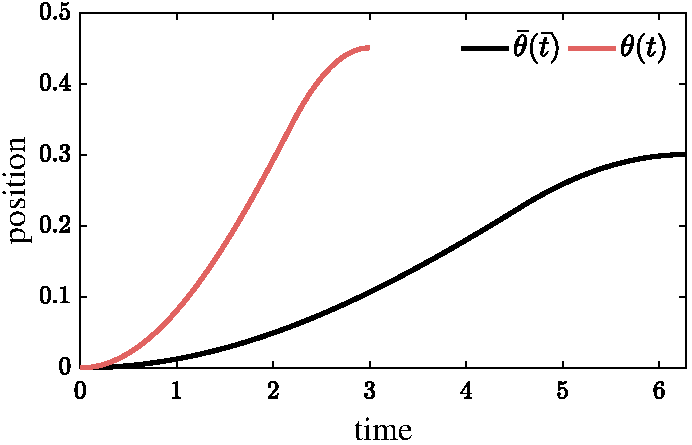
\includegraphics[width=\textwidth]{../ch4/figures/sasa_position}
    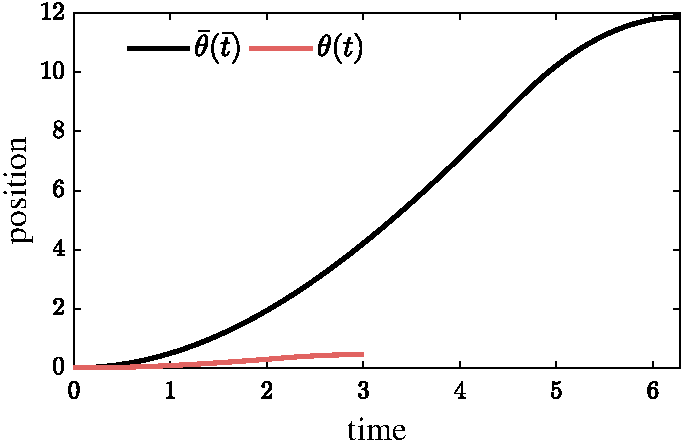
\includegraphics[width=\textwidth]{../ch4/figures/TP3_position}
    \caption{$\theta(t)$ and $\bar{\theta}(\bar{t})$.}
\end{subfigure}%
\begin{subfigure}[b]{0.5\columnwidth}
    \centering
    % 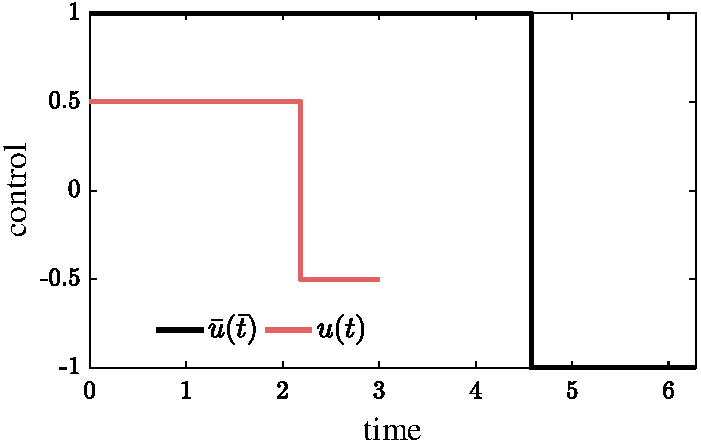
\includegraphics[width=\textwidth]{../ch4/figures/sasa_control}
    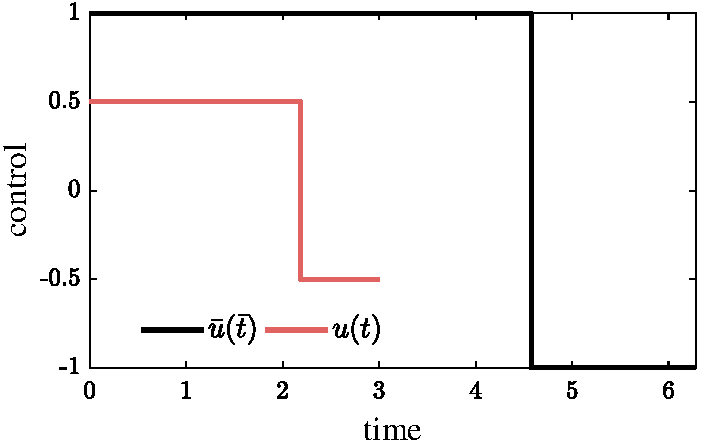
\includegraphics[width=\textwidth]{../ch4/figures/TP3_control}
    \caption{$u(t)$ and $\bar{u}(\bar{t})$.\label{fig:ch4:sasa_control}}
\end{subfigure}
\caption[Scaled and unscaled solutions for the simple SASA problem]{Scaled and unscaled solutions for the simple SASA problem with $u_{\max} = 0.5$, $t_f = 3$, $J = 3$.\label{fig:ch4:sasa_plots}}
\end{figure}


With the optimization problem, optimality conditions, and optimal solutions thoroughly characterized, we can compare this simple SASA problem to the original design study in Ref.~\cite{Chilan2017a}. Both the scaled and unscaled solutions for the simple SASA problem without the additional bound on the period being active are shown in Fig.~\ref{fig:ch4:sasa_plots}.
There are a number of similarities between the trajectories in Ref.~\cite{Chilan2017a} and in Fig.~\ref{fig:ch4:sasa_plots}, including the bang-bang nature of the control when the period constraint is not active, and the general shape of the bus angle trajectories.

% new pargraph
The primary comparison is Fig.~\ref{fig:ch4:sasa_comparison}, which includes the results from Fig.~10 of Ref.~\cite{Chilan2017a}.
The figure plots the natural period of the first mode vs. $t_f$.
There is an observed linear trend until a period limit seems to be reached.
This is present for both design representations used: \glsfoo[noindex]{PLS} and \glsfoo[noindex]{VL}.
Both of these representations can change the structural properties of the solar array.
Although it is tough to see in the figure, there are coinciding data points at $t_f=0.12$ s for both cases indicating that there is a similar optimal value for $T_1$ (and ratio).

\begin{figure}
\centering
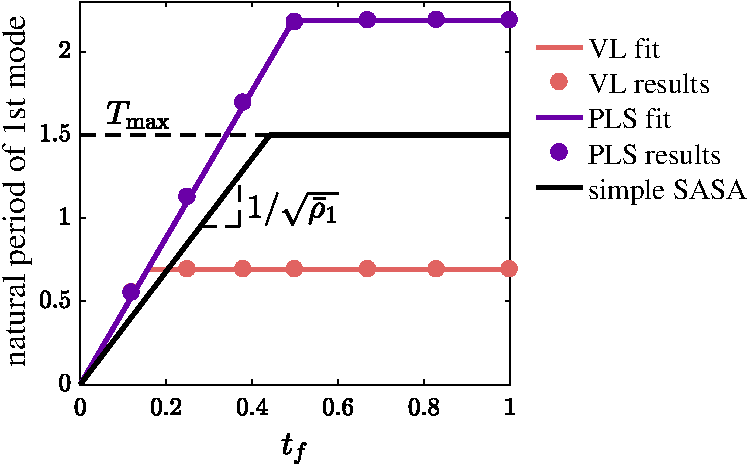
\includegraphics[width=0.6\textwidth]{../ch4/figures/sasa_comparison}
\caption[Natural period vs.~$t_f$ for the simple SASA and original design study]{Natural period vs.~$t_f$ results for the simple SASA problem and original design study in Chapter~\ref{ch:7}.\label{fig:ch4:sasa_comparison}}
\end{figure}

% new paragraph
Observing Fig.~\ref{fig:ch4:sasa_comparison}, there is a direct parallel between the data points and the simple SASA problem.
For the scaled problem, $\bar{\rho}_1^\dagger = 0.0866$ while the results from Ref.~\cite{Chilan2017a} indicate $\bar{\rho}_1$ should be approximately $0.0513$.
The difference may be attributed to the representation and constraints in the original design study.
Initial discussions of the results tried to pin the ratio $t_f/T_1$ to $1/4$ due to the periodic resonance of a simple beam.
However, the simple SASA problem suggests that this ratio is simply an arbitrary constant dependent on the interaction between the bang-bang controller and dynamics.
Continuing with the comparisons, the $T_{\max}$ bound seems to equal about $2.19$ s for the PLS case and $0.69$ s for the VL case.
If the physical-system constraints could be lifted, we have a reasonable prediction for how $T_1$ should vary.

% new paragraph
This example illustrated how scaling can be utilized effectively to obtain insights in a design study.

\subsection{Example 2: Co-Design Transfer Problem \label{sec:ch4:transfer}}

In this example, we will use scaling to transform a co-design problem into a form with a known solution\footnote{This problem was also used in Sec.~\ref{sec:ch3:transfer}.}. Consider the following co-design problem:
\begin{subequations}
\label{eq:ch4:ex2_prob_1}
\begin{align}
\min_{k, u(t)}  \quad & \int_{0}^{t_f} u^2 dt \\
\text{subject to:} \quad & \ddot{y} = - k y + u \\
& y(0) = y_0, \ \dot{y}(0) = v_0, \ y(t_f) = 0, \ \dot{y}(t_f) = 0
\end{align}
\end{subequations}

\noindent where $k$ is the time-independent, physical-system design variable and $u(t)$ is the open-loop control design variable.
Through scaling, we can transform Prob.~(\ref{eq:ch4:ex2_prob_1}) above into the problem in Ref.~\cite[pp.~166--167]{Bryson1975a}. 
To accomplish this, consider the following change of variables:
\begin{gather}
\label{eq:ch4:ex2_rules}
t = \alpha_t \bar{t}, \quad u = \alpha_u \bar{u}
\end{gather}

\begin{figure*}[t]
\centering
% \includegraphics[options]{name}

\begin{subfigure}[b]{0.5\textwidth}
    \centering
    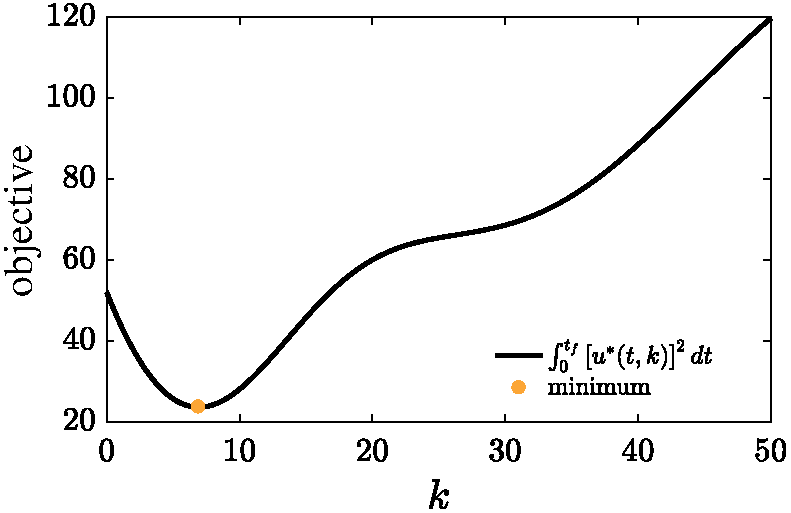
\includegraphics[width=\textwidth]{../ch4/figures/transfer_psi}
    \caption{Objective function values.}
\end{subfigure}

\begin{subfigure}[b]{0.4\textwidth}
    \centering
    \includegraphics[width=\textwidth]{../ch4/figures/transfer_u}
    \caption{$u^*(t,k)$ for various values of $k$.}
\end{subfigure}%
\begin{subfigure}[b]{0.4\textwidth}
    \centering
    \includegraphics[width=\textwidth]{../ch4/figures/transfer_x}
    \caption{$y^*(t,k)$ for various values of $k$.}
\end{subfigure}

\caption[Co-design transfer problem]{Co-design transfer problem with $t_f = 1$, $x_0 = 1$, and $v_0 = 2$ (with $k^* = 6.924$).\label{fig:ch4:transfer_solution}}
\end{figure*}

\noindent We choose the following values for the scaling constants:
\begin{gather}
\alpha_t = \frac{1}{\sqrt{k}}, \quad \alpha_u = k
\end{gather}

\noindent where $k>0$. The case for $k=0$ needs to be handled separately.
Substituting in these scaling laws results in the following problem formulation:
\begin{subequations}
\label{eq:ch4:ex2_prob_2}
\begin{align}
\min_{k, \bar{u}(\bar{t})} \quad &  k^{3/2} \int_{0}^{\bar{t}_f} \bar{u}^2 d\bar{t} \\
\text{subject to:} \quad & y'' = - y + \bar{u} \\
& y(0) = y_0, \quad y'(0) = \bar{v}_0 \\ 
& y(\bar{t}_f) = 0, \quad y'(\bar{t}_f) = 0 \\
\text{where:} \quad & \bar{t}_f = \sqrt{k} t_f, \bar{v}_0 = v_0/\sqrt{k}
\end{align}
\end{subequations}

The solution to Prob.~(\ref{eq:ch4:ex2_prob_2}) above is readily available in Ref.~\cite{Bryson1975a}. Using this result and applying the scaling rules in Eqn.~(\ref{eq:ch4:ex2_rules}), we obtain the following solution for $u(t)$ as a function of $k$:
\begin{align}
\label{eq:ch4:ex2_usol}
\begin{aligned}
u^*(t,k) &= - \frac{2k}{k t_f^2 - \sin^2(\sqrt{k} t_f)} \left( c_1(t,k) x_0 + c_2(t,k) \frac{v_0}{\sqrt{k}} \right) \\
c_1(t,k)  &= \sin\left( \sqrt{k}(t_f - t) \right)\sin\left(\sqrt{k}t_f\right) - \sqrt{k} t_f \sin \left(\sqrt{k}t \right) \\
c_2(t,k)  &= - \cos\left(\sqrt{k}(t_f-t)\right) \sin\left(\sqrt{k}t_f\right) + \sqrt{k} t_f \cos\left(\sqrt{k}t\right)
\end{aligned}
\end{align}

\noindent For certain problem parameter values, the solution for various values of $k$ is shown in Fig.~\ref{fig:ch4:transfer_solution}. 
The original objective function can now be computed analytically with Eqn.~(\ref{eq:ch4:ex2_usol}).
With this closed-form expression for the objective function, an optimality condition for $k$ can be derived.
This property makes this problem quite suitable for investigations between nested and simultaneous co-design methods and can be used to illustrate a number of concepts found in many co-design problems (such as open-loop control, multiple optima, degenerate plant designs, and a system-level objective function) \cite{Herber2017b}.

% new paragraph
For many DO problems, obtaining a closed-form solution for a portion of the design variables may not be possible. 
Observing different (but equivalent) forms of the same design optimization formulation can facilitate a better understanding of the design problem.
In this example, we see that for larger values of $k$, the scaled problem has a larger time horizon but smaller initial velocity. 

% new paragraph
In addition, these different forms may be more suitable computation depending on the parameter values.
In this example using the original Prob.~(\ref{eq:ch4:ex2_prob_1}) formulation, large values of $k$ would result in highly oscillatory solutions.
With the time-horizon fixed, large discretization errors would start appearing in the solutions with a fixed number of time points if a DT solution method was utilized. This helps motivate the final example.

\subsection{Example 3: Direct Transcription Discretization \label{sec:example3}}

DT is a popular solution method for solving DO problems and is described in more detail in Chapter~\ref{ch:5} \cite{Biegler2010a, Betts2010a, Allison2014b,Allison2014a}.
In this approach, the dynamics are approximated with a large number of equality constraints, termed defect constraints.
Equality constraints in a NLP are typically of the form $h(\bm{x}) = 0$. However, most numerical algorithms implement this constraint type as two inequality constraints as:
\begin{align}
\label{eq:ch4:ineq_error}
- \epsilon \leq h(x) \leq \epsilon
\end{align}

\noindent where \gls{epsilon} is a small tolerance number (e.g.,~the default tolerance in \textsc{Matlab}'s \texttt{fmincon} function is $\epsilon = 10^{-6}$ \cite{matlab-fmincon}).
In this example, we will demonstrate how the absolute magnitudes of the state variables can greatly degrade direct transcription approximations.

Consider the simple scalar system:
\begin{align}
\label{eq:ch4:dt_original}
\dot{y} = a y, \quad y(0) = y_0
\end{align}

\noindent where the solution to this set of DAEs is $\hat{y}(t) = y_0 e^{at}$. We can introduce a change of variables as:
\begin{align*}
t = \alpha_t \bar{t}, \quad y = \alpha_y \bar{y}
\end{align*}

\noindent where the scaling constants are $\alpha_t = \abs{a}$ and $\alpha_y = y_0$, resulting in the following scaled system:
\begin{align}
\bar{y}' = \bar{y}, \quad \bar{y}(0) = 1
\end{align}

\noindent We can now see how the relative error is influenced by the different systems.

% new paragraph
A basic single-step DT method is the trapezoidal rule and the defect constraint that ensures accurate dynamics has the following form for a scalar ODE:
\begin{align}
\label{eq:ch4:defect}
0 &= y_k - y_{k-1} - \frac{\Delta_k}{2}\Big( f(t_{k-1}, y_{k-1}) + f(t_k, y_{k}) \Big)
\end{align}

\noindent where $y_k$ is the approximate value of $y(t)$ at $t_k$, $\glsfirst{stepsize}_k = t_k - t_{k-1}$ is the step-size parameter, and $f(t_k, y_{k})$ is the value of the derivative function at $t_k$.

We will consider the initial step, i.e.,~$k=1$. Then the DT constraint for Eqn.~(\ref{eq:ch4:dt_original}) is:
\begin{align}
0 &= y_1 - y_{0} - \frac{\Delta_1}{2} \left( a y_{0} + a y_1 \right)
\end{align}

Using the tolerances in Eqn.~(\ref{eq:ch4:ineq_error}), we can derive the minimum and maximum values for $y_1$ that still satisfy the constraint:
\begin{align}
\frac{\left(1+\Delta_1 a/2\right) y_0 - \epsilon}{\left(1-\Delta_1 a/2\right)} \leq y_1 \leq \frac{\left(1+\Delta_1 a/2\right) y_0 + \epsilon}{\left(1-\Delta_1 a/2\right)}
\end{align}

\noindent Alternatively, the bounds for $\bar{y}_1$ are:
\begin{align}
\frac{\left(1+\mathrm{sign}(a)\Delta_1/2\right) - \epsilon}{\left(1-\mathrm{sign}(a)\Delta_1/2\right)} \leq \bar{y}_1 \leq \frac{\left(1+\mathrm{sign}(a)\Delta_1/2\right) + \epsilon}{\left(1-\mathrm{sign}(a)\Delta_1/2\right)}
\end{align}

\noindent The relative error is defined as:
\begin{align}
\gls{relerror} = \frac{y_1 - \hat{y}_1}{\hat{y}_1} = \frac{y_1 - y_0 e^{a t_1}}{y_0 e^{a t_1}}, \quad \bar{e}_r = \frac{\bar{y}_1 - e^{\mathrm{sign}(a) t_1}}{ e^{\mathrm{sign}(a) t_1}}
\end{align}

Now, consider the following values for the problem and DT parameters: $y_0 = 10^{-6}$, $a = 2$, $\epsilon = 10^{-6}$, $\Delta_1 = 10^{-3}$. For these values, we have the following relative error bounds:
\begin{subequations}
\begin{gather}
-9.99 \times 10^{-1} \leq e_r \leq 9.99 \times 10^{-1} \\
-9.99 \times 10^{-7} \leq \bar{e}_r \leq 9.99 \times 10^{-7}
\end{gather}
\end{subequations}

\noindent We see that the $e_r$ is quite poor using the original system while $\bar{e}_r$ is right around the expected $\epsilon$ tolerance. Consider one more choice of parameters: $y_0 = 10^{3}$, $a = -1$, $\epsilon = 10^{-6}$, $\Delta_1 = 10^{-3}$ and error bounds: 
\begin{subequations}
\begin{gather}
-1.08 \times 10^{-9} \leq e_r \leq 9.13 \times 10^{-10} \\
-1.00 \times 10^{-6} \leq \bar{e}_r \leq 1.00 \times 10^{-6}
\end{gather}
\end{subequations}

\begin{figure}
\centering
\begin{subfigure}[b]{0.5\textwidth}
    \centering
    \includegraphics[width=\textwidth]{../ch4/figures/dt_errors_1}
    \caption{$y_0 = 10^{-6}$ and $a = 2$.\label{fig:ch4:dt_errors_1}}
\end{subfigure}%
\begin{subfigure}[b]{0.5\textwidth}
    \centering
    \includegraphics[width=\textwidth]{../ch4/figures/dt_errors_2}
    \caption{$y_0=10^2$ and $a=-1$.\label{fig:ch4:dt_errors_2}}
\end{subfigure}
\caption[Maximum absolute relative error vs. step size for defect constraints]{Maximum absolute relative error vs. step size for original and scaled defect constraints.\label{fig:ch4:dt_errors}}
\end{figure}


\noindent Now we see that the relative error bounds are tighter than $\epsilon$ which could lead to numerical issues. The scaled form, however, is still right around the $\epsilon$ tolerance. The maximum absolute relative error vs. step size is shown in Fig.~\ref{fig:ch4:dt_errors}. From these plots, we see that for a sufficiently small step size, the scaled system has error bounds near $\epsilon$.

Both of these parameter sets show the importance of scaling the dynamics to be near unity when using a DT implementation.
Since DT implementations use a large number of linked defect constraints, the errors can compound, potentially producing highly inaccurate results.
Additionally, scaling the time horizon provides a more uniform method for selecting $\Delta$ to achieve suitable accuracy without too many optimization variables (note that $\Delta_1=10^{-3}$ for $\bar{e}_r$ is quite good in both plots). Finally, scaling the states to be near unity is also produces computationally favorable matrices (Hessian/Jacobians) and finite differencing \cite{Rao2010a, Betts2010a}.

\section{Summary\label{sec:ch4:conclusion}}

In this chapter, we explored scaling in DO with a particular focus on how to leverage scaling in design optimization.
A review of the large amount of work around scaling was provided.
The necessary theory for scaling DO formulations was presented and a number of novel motivating examples were provided.
Scaling was shown to help facilitate finding accurate, generalizable, and intuitive information.

% new paragraph
At a basic level, scaling is simply the stretching, squeezing, and shifting of the problem elements such as the time continuum, design variables, constraints, and objective function. 
The unique structure of DO suggests that scaling can be utilized in novel ways to provide better analysis and formulations more favorable for different solution methods.
The mechanics of scaling are fairly straightforward but proper utilization of scaling is heavily reliant on the creativity and intuition of the designer.
This nebulous qualification is the primary limitation on the use of scaling. However, scaling is also limited by the scaling law chosen, the structure of the problem, and the number of free parameters.
Furthermore, scaling does not remove optimization; we still need to solve some form of the optimization problem.
Improper use of scaling can lead to incorrect solutions/insights or amplification of numerical issues rather than mitigation.

% new paragraph
Aiding the designer in constructing the appropriate scaled formulations needs compelling examples.
In the simple SASA problem, scaling was used to understand observed results from more complete, higher-fidelity design study. The simpler scaled optimization problem and dimensionless variables provided a number of insights. 
In the second example, the solution to a co-design problem was found by leveraging a scaled formulation with the known solution.
Observing different (but equivalent) forms of the same design optimization formulation can facilitate a better understanding of the design problem.
In the final example, the discretization error of one of the popular solution methods (namely direct transcription) for DO was explored. The scaled system showed much more favorable properties than the original.
Additional work is needed to develop general guidelines to aid in balancing the many uses of scaling. % scaling
\mychapterfoot{\label{ch:dt}Direct Transcription and Linear-Quadratic Dynamic Optimization\label{ch:5}}

\footnotetext{Elements of this chapter are based on work completed in Ref.~\cite{manuscript-dt-qp}.}

%--- epigraph
\epigraph{\textit{``Since all the effects of Nature follow a certain law of maxima or minima, there is no doubt that, on the curved paths, which the bodies describe under the action of certain forces, some maximum or minimum property ought to obtain. What this property is, nevertheless, does not appear easy to define \textit{a priori} by proceeding from the principles of metaphysics;''}}{\textmd{L. Euler} \cite[p.~106]{Goldstine1980a}}
%--- epigraph

Direct transcription is a solution strategy discussed briefly in Chapters~\ref{ch:3} and \ref{ch:4} for finding approximate solutions to dynamic optimization problems.
This chapter focuses on a particular subclass that is relevant to the two case studies in Chapters~\ref{ch:7} and \ref{ch:8}.
Both use the nested co-design strategy from Chapter~\ref{ch:3} so many control subproblems need to be solved and efficiency is paramount.
The methods developed in this chapter provide a single unified description to automatically generate and solve this class of problems, even if there are different architectures with a varying number of states and controls.

%-------------------------------------------------------------------
\section{Introduction}

For more than half a century, dynamic optimization, or optimization with time-varying quantities, has played an integral role in the advancement of many designed systems, including applications in chemical engineering \cite{Biegler2010a}, aerospace engineering \cite{Betts2010a}, wave energy conversion \cite{Faedo2017a}, and finance/economics \cite{Deissenberg2005a}.
\Glsfirst{NLDO} represents the most general class of problems \cite{Betts2010a, Biegler2010a, Bryson1975a}.
A subclass of NLDO is \glsfirst{LQDO} where certain elements of the formulation are limited to quadratic and linear functions \cite{Bryson1975a, Anderson2007a, Liberzon2012a}. 
Frequently, \lqdo{} formulations used in the literature are only a subclass of the general \lqdo{} problem.
The key feature shared between the \lqdo{} formulations is that solutions may be found via an appropriate \glsfoo[noindex]{QP}, a particular class of finite-dimensional mathematical programs \cite{Boyd2009a}.
Here we present a unified framework for \lqdo{} that can be solved as {\qp}s.

% new paragraph
In addition to providing a clear delineation of the general \lqdo{} problem class, we develop an \glsfirst{APGP} to form the {\qp}s that represent \lqdo{} problems.
Here we define an \apgp{} as a procedure in which, given a natural and manageable description of the problem, one can obtain a numerical solution with little or no user expertise.
A key to minimizing the amount of knowledge needed by the user is an automated and efficient implementation of the various solution methods.
Such procedures are available for DO (e.g.,~\textsc{gpops-ii} \cite{Patterson2014a}, \textsc{psopt} \cite{Becerra2015a}, \textsc{propt} \cite{Rutquist2010a}, \textsc{sos} \cite{SOS2015a}, and \textsc{dircol} \cite{Stryk1999a}) but typically are developed for the more general NLDO problems and therefore cannot effectively leverage the structure of \lqdo.
For the {\apgp}s that handle \lqdo{} problems, they are limited to specific solution methods and problem formulations (e.g.,~\textsc{mpt3} \cite{Herceg2013a} and \textsc{mpc toolbox} \cite{matlab-mpc}).
Manual implementation of these solution methods is still quite prevalent in the literature, perhaps due to the lack of the necessary tools which sufficiently address the challenges of the particular class of problems.
Additionally, a wide variety of competing solution methods exist, and comparisons between them cannot typically be performed efficiently (especially if a manual implementation is needed).
These issues limit productivity and the general reach of \lqdo, but can be addressed using an \apgp{} under a unified framework for \lqdo. 
In addition, this unified framework also provides additional insights into the \lqdo{} problem class and led to additional developments in the solution methods. 

% new paragraph
The remainder of the chapter is structured as follows.
Section~\ref{sec:ch5:lqdo} presents the general problem formulation for \lqdo.
Next, Sec.~\ref{sec:ch5:lqdo} discusses formulating \lqdo{} problems as {\qp}s with direct transcription methods. 
Section~\ref{sec:ch5:algorithm} details the \apgp{} which takes a natural and manageable description of the problem and forms the \qp.
Section~\ref{sec:ch5:extensions} outlines some extensions to the original \lqdo{} problem formulation.
Section~\ref{sec:ch5:examples} assesses the \apgp{} with a number of numerical examples.
Section~\ref{sec:ch5:future:work} discusses various future work items.

%-------------------------------------------------------------------
\section{Linear-Quadratic Dynamic Optimization} \label{sec:ch5:lqdo}

In this section, we begin by describing the general NLDO formulation and then a \qp{} is defined. Then, with an assumed property of the solution method, we will characterize the \lqdo{} formulation that supports solution via {\qp}s.

%-------------------------------------------------------------------
\subsection{General Nonlinear Dynamic Optimization} \label{sec:ch5:gnldo}

% Brief statement of general nonlinear optimal control
Dynamic-system design permits the optimization of: control trajectories, $\gls{olc}(t)$; static parameters, $\gls{parameters}$; and the time horizon defined by the boundary values $\gls{time}_{\glsfoo[noindex]{initial}}$ and $t_{\glsfoo[noindex]{final}}$. Written as an infinite-dimensional mathematical program, the NLDO formulation is:%
\begin{subequations}%
\label{eq:ch5:NLDO}
\begin{align}
\min_{\bm{u}(t),\bm{p},t_0,t_f} \qquad& \gls{objective} = \int_{t_0}^{t_f} \mathcal{L} \big(t,\bm{\xi}(t),\bm{u}(t), \bm{p} \big) dt + \mathcal{M}\big(\bm{p}, t_0, \bm{\xi}(t_0), t_f, \bm{\xi}(t_f) \big) \label{eq:ch5:NLobj} \\
\text{subject to:} \qquad &  \hspace{0.0in} 
\dot{\bm{\xi}}(t) - \glsname{f}\big(t, \bm{\xi}(t), \bm{u}(t), \bm{p} \big) = \bm{0} \label{eq:ch5:NLdyn} \\
& \gls{equality}\big(t, \bm{\xi}(t), \bm{u}(t), \bm{p}, t_0, \bm{\xi}(t_0), t_f, \bm{\xi}(t_f) \big) = \bm{0}  \label{eq:ch5:NLeq} \\
& \gls{inequality}\big(t, \bm{\xi}(t), \bm{u}(t), \bm{p}, t_0, \bm{\xi}(t_0), t_f, \bm{\xi}(t_f) \big) \leq \bm{0}  \label{eq:ch5:NLineq}
\end{align}
\end{subequations}%

\noindent where Eqn.~(\ref{eq:ch5:NLobj}) defines the objective function with Lagrange $\gls{lagrange}$ and Mayer $\gls{mayer}$ terms.
Equation~(\ref{eq:ch5:NLdyn}) enforces the first-order \glsfoo[noindex]{ODE} that describes the dynamic behavior of the states $\gls{states}(t)$.
Equation~(\ref{eq:ch5:NLeq}) enforces the algebraic equality constraints, and Eqn.~(\ref{eq:ch5:NLineq}) enforces the algebraic inequality constraints.
Most NLDO problems only contain certain elements of this general formulation.
Many presentations of general NLDO reorganize Eqns.~(\ref{eq:ch5:NLeq})--(\ref{eq:ch5:NLineq}) by partitioning the constraints into those which depend on time-varying quantities and those which do not.
The time-varying constraints are termed \textit{path} constraints, and time-independent constraints termed \textit{boundary} constraints (as was done in Chapters~\ref{ch:3} and \ref{ch:4}) \cite{Betts2010a, Biegler2010a, Herber2014a}.
Some formulations also include the states as optimization variables (primarily motivated by the eventual solution method and the states are still constrained by Eqn.~(\ref{eq:ch5:NLdyn})).

\subsection{Quadratic Program}

In this chapter, we are concerned with a subclass of Prob.~(\ref{eq:ch5:NLDO}) that can be solved numerically as a finite-dimensional \qp. A \qp{} is defined as:%
\begin{subequations}%
\label{eq:ch5:basicQP}
\begin{align}
\min_{\gls{xqp}} \qquad& \frac{1}{2}\mathbf{X}^{\glsfirst{transpose}} \gls{hqp} \mathbf{X} + \gls{fqp}\tran \mathbf{X} + \gls{cqp} \label{eq:ch5:qpH} \\
\text{subject to:} \qquad& \gls{Aqp}_{\glsfirst{noteq}} \mathbf{X} = \gls{Bqp}_{e} \label{eq:ch5:Ae} \\
& \mathbf{A}_{\glsfirst{notineq}} \mathbf{X} \leq \mathbf{B}_{i} \label{eq:ch5:Ai} \\
& \myunderbar{\mathbf{X}\gls{myunderbar}} \leq \mathbf{X} \leq \myoverbar{\mathbf{X}\gls{myoverbar}} \label{eq:ch5:qpbounds}
\end{align}
\end{subequations}%

\noindent where $\mathbf{X}$ is the set of optimization variables, and all other terms in the formulation are real-valued with no dependence on $\mathbf{X}$.
$\mathbf{H}$ is known as the Hessian matrix and is symmetric.
We note that the \qp{} formulation in Prob.~(\ref{eq:ch5:basicQP}) is decidedly more structured than NLDO formulation in Prob.~(\ref{eq:ch5:NLDO}).
The optimal solution to a quadratic program exists and is the global optimum if the objective is a convex quadratic function and the feasible set of Prob.~(\ref{eq:ch5:basicQP}) is nonempty \cite{Pang1983a}.
There are a variety of efficient algorithms for solving {\qp}s, including  active-set \cite{Pang1983a}, interior-point \cite{Altman1999a}, and augmented Lagrangian \cite{Delbos2005a} methods.

\subsection{Linear-Quadratic Dynamic Optimization Problem Formulation} \label{sec:ch5:lqdoform}

In this section, a subclass of Prob.~(\ref{eq:ch5:NLDO}) is defined that, when combined with a solution method, can generate a \qp{} in the form of Prob.~(\ref{eq:ch5:basicQP}) that approximates the infinite-dimensional solution. 
There are two aspects that determine if a particular infinite-dimensional problem can be formulated as \qp: 1) the structure of the objective function and constraints in Prob.~(\ref{eq:ch5:NLDO}), and 2) the solution method that approximates the infinite-dimensional problem as a finite one.
To address the latter aspect, we will only consider order-maintaining methods.
An order-maintaining method, for example, would have the following property: if a term is linear in the infinite-dimensional problem, then it will be approximated as a set of variables that appear linearly in the finite-dimensional problem.
An equivalent property will need to be true for quadratic terms.

First, we denote the vector of optimization variables as:
\begin{align}\label{eq:ch5:x:cont}
\gls{x} = \begin{bmatrix} \bm{u} \\ \bm{\xi} \\ \bm{p} \end{bmatrix}
\end{align}

\noindent Both elements of the time horizon are missing because they do not permit {\qp}s (see Sec.~\ref{sec:ch5:mtp}).
In addition, the states are included to support proper analysis of the problem class and the eventual solution methods.
We also see $\bm{\xi}(t_0)$ and $\bm{\xi}(t_f)$ directly in the formulation, so we define an expanded set of optimization variables as:
\begin{align} \label{eq:ch5:varindices}
\gls{expanded} = \begin{lbmatrix}{1} \bm{x}_c \\ \bm{x}_d \end{lbmatrix} \ \text{where:} \ \ 
\bm{x}_c = \begin{lbmatrix}{1} \bm{u} \\ \bm{\xi} \end{lbmatrix}
:= \begin{lbmatrix}{1} \bm{x}_1 \\ \bm{x}_2 \end{lbmatrix} \  \text{and} \ \ 
\bm{x}_d = \begin{lbmatrix}{1} \bm{p} \\ \bm{\xi}(t_0) \\ \bm{\xi}(t_f) \end{lbmatrix}
:= \begin{lbmatrix}{1} \bm{x}_3 \\ \bm{x}_4 \\ \bm{x}_5 \end{lbmatrix}
\end{align}

\noindent where $\bm{x}_{\glsfirst{continuous}}$ and $\bm{x}_{\glsfirst{discrete}}$ are collections of the continuous (infinite-dimensional) and discrete (finite-dimensional) optimization variables, and indexed variables $\bm{x}_i$ are equivalent to the variable in the same row in the vector directly to the left in the same equation (e.g.,~$\bm{u} := \bm{x}_1$). 

%-------------------------------------------------------------------
\subsubsection{Linear Dynamics}

A good place to start is with the dynamics expressed in Eqn.~(\ref{eq:ch5:NLdyn}) as it is a unique feature of DO. An appropriate choice for the state dynamics is a linear nonhomogeneous differential equation:
\begin{align} \label{eq:ch5:fdyn}
\bm{f} = \bm{f}^{\glsfirst{notqp}} := \gls{dynA}(t)\bm{\xi}(t) + \gls{dynB}(t) \bm{u}(t) + \gls{dynG}(t)\bm{p} + \gls{dynd}(t) 
\end{align}

\noindent where $\{\bm{A},\bm{B},\bm{G}\}$ are the \glsfirst{LTV} state/input/parameter matrices and $\bm{d}(t)$ is a disturbance.

Many authors consider different variations on Eqn.~(\ref{eq:ch5:fdyn}).
The simplest form is that of a \glsfirst{LTI} system: $\bm{f} = \bm{A}\bm{\xi} + \bm{B} \bm{u}$ \cite{Lack1967a, Sala2007a}.
The next most common form is the LTV system without $\bm{G}$ or $\bm{d}$ \cite{Wang1992a}.
The addition of the disturbance does appear in a number of formulations \cite{Hampton1996a, Popescu2009a, Li2015a, Bryson1975a, Han2012a}.
No general formulations are seen which include $\bm{p}$, but this may be due to the limited number of problems where $\bm{p}$ shows up linearly in $\bm{f}$. 
However, this demonstrates that even the simplest mixed parameter-control problems are not \lqdo{} problems \cite{Herber2014a}.
A more general form is $\gls{dynE}(t)\dot{\bm{\xi}} = \bm{f}^{QP}$, known as descriptor form \cite{Gerdts2015a, Campbell2013a}.
Here we will only consider that case where $\bm{E}$ is nonsingular so it may be written as $\dot{\bm{\xi}} = \bm{E}^{-1}\bm{f}^{QP}$. 

One may be tempted to integrate this differential equation and would arrive at the following:
\begin{align} \label{eq:ch5:statesol}
\bm{\xi}(t) = \bm{\Phi}(t,t_0) \bm{\xi}(t_0) + \int_{t_0}^{t}  \bm{\Phi}(t,\tau) \big( \bm{B}(\tau) \bm{u}(\tau) + \bm{G}(\tau) \bm{p} + \bm{d}(\tau) \big) d\tau
\end{align}

\noindent where $\gls{transition}$ is the state-transition matrix which describes the dynamics of the homogeneous system (i.e.,~the integral in Eqn.~(\ref{eq:ch5:statesol}) is zero) \cite{Chen1999a}.
The most general transition matrix is given by the Peano-Baker series.
However, if $\bm{A}$ is time-invariant, then the state-transition matrix is $e^{\bm{A}(t-\tau)}$.
Some solution methods will utilize these properties, but in general, the differential equation is challenging to utilize directly.

%-------------------------------------------------------------------
\subsubsection{Quadratic Objective Function}

The \qp{} objective function in Eqn.~(\ref{eq:ch5:qpH}) is a polynomial with degree two; therefore, we will choose a general quadratic cost functional containing appropriate elements of $\tilde{\bm{x}}$:%
\allowdisplaybreaks[1]%
\begin{gather} \label{eq:ch5:QOFLagrange}
\mathcal{L} = \mathcal{L}^{QP} := 
\underbracket{\sum_{i=1}^5 \sum_{j=1}^5 \bm{x}_i\tran  \gls{Lbm}_{ij}(t) \bm{x}_j}_{\textstyle H^{\mathcal{L}} = \tilde{\bm{x}}\tran  \bL \tilde{\bm{x}} }
\ + \
\underbracket{\sum_{j=1}^5 \gls{lbm}_j\tran (t) \bm{x}_j}_{\textstyle F^{\mathcal{L}} = \bl\tran   \tilde{\bm{x}}}
\ + \
c^{\mathcal{L}}(t) \\ \label{eq:ch5:QOFMayer}
\mathcal{M} = \mathcal{M}^{QP} := 
\underbracket{\sum_{i=3}^5 \sum_{j=3}^5 \bm{x}_i\tran \gls{Mbm}_{ij} \bm{x}_j}_{\textstyle H^{\mathcal{M}} = {\bm{x}}\tran_d \bM {\bm{x}}_d }
\ + \
\underbracket{\sum_{j=3}^5 \gls{mbm}\tran_j \bm{x}_j}_{\textstyle F^{\mathcal{M}} = \bmm\tran  \bm{x}_d}
\ + \
c^{\mathcal{M}}
\end{gather}
\allowdisplaybreaks[0]%

\noindent where we require that $\bL_{ij} = \bL_{ji}\tran$ and $\bM_{ij} = \bM_{ji}\tran$ so that both are symmetric since $\mathbf{H}$ needs to be symmetric.
We note that the Mayer term only includes the discrete optimization variables because including any element of $\bm{x}_c$ would not result in a scalar quantity\footnote{We can also note that since the time horizon is fixed in \lqdo, $\mathcal{M}$ is redundant since $\bm{M}_{ij}/(t_f-t_0)$ could be added to $\bm{L}_{ij}$ for the appropriate indices.
To facilitate more natural descriptions, all terms are considered.}.

The Lagrange and Mayer terms in Eqns.~(\ref{eq:ch5:QOFLagrange})--(\ref{eq:ch5:QOFMayer}) include all possible time-varying quadratic and linear terms in the most general expression.
While most of the applications utilize a few select time-variant and time-invariant terms for their performance index \cite{Hampton1996a, Popescu2009a, Campbell2013a, Gerdts2015a, Tang2007a, Jerez2011a, Bashein1971a}, there are a few applications in the literature which include all the time-varying $\bm{x}_c$ dependent terms in the linear and quadratic terms, but only includes $\bm{\xi}(t_f)$ terms in linear and quadratic Mayer terms \cite{Wang1992a, Sideris2010a, Han2012a}.
Constants in Lagrange and Mayer terms ($c^{\mathcal{L}}$ and $c^{\mathcal{M}}$) are not widely used, but $c^{\mathcal{M}}$ term appears in a few references \cite{Gerdts2015a}.
We also note that if there are no quadratic terms (i.e.,~$\bm{L}=\bm{0}$ and $\bm{M}=\bm{0}$), then the \lqdo{} problem can be solved with linear programming (a special case of quadratic programming) \cite{Boyd2009a}.

%-------------------------------------------------------------------
\subsubsection{Additional Linear Constraints} 

In most DO problems there are additional constraints that need to be enforced.
In the context of \lqdo, these can all be expressed as the following general linear equality and inequality constraint forms:%
\allowdisplaybreaks[1]%
\begin{gather}
h = h^{QP} := \sum_{j=1}^5 \gls{Ybm}_{j}(t)\tran \bm{x}_j - \hat{Y}(t) = \bm{Y}\tran \tilde{\bm{x}} - \hat{Y} = 0 \label{eq:ch5:hqp} \\
g = g^{QP} := \sum_{j=1}^5 \gls{Zbm}_{j}(t)\tran \bm{x}_j - \hat{Z}(t) = \bm{Z}\tran \tilde{\bm{x}} - \hat{Z} \leq 0 \label{eq:ch5:gqp}
\end{gather}%
\allowdisplaybreaks[0]%

\noindent This representation of the constraints mixes the path and boundary definitions mentioned in Sec.~\ref{sec:ch5:gnldo}. In Sec.~\ref{sec:ch5:alg:lin:constraints} it will be shown that a straightforward procedure exists to determine which class (path or boundary) is most appropriate for a specified constraint. 

As with the previous \lqdo{} elements, there are a number of common constraint types seen in literature that are captured by these general linear constraints.
There is a broad class of boundary condition constraints that only contain the initial and final states \cite{Gerdts2015a} including prescribed initial conditions \cite{Lack1967a, Bryson1975a, Wang1992a, Anderson2007a, Tang2007a, Sideris2010a, Han2012a}, prescribed final or terminal conditions \cite{Lack1967a, Bashein1971a, Bryson1975a, Jerez2011a}, and periodic conditions \cite{Herber2014a}.
Initial and final state conditions need not be only equality constraints \cite{Jerez2011a}. Mixed control-state constraints are also possible \cite{Sideris2010a, Bryson1975a, Gerdts2015a, Jerez2011a, Han2012a}.
This type of constraint commonly includes only $\bm{x}_c$ terms, but the whole collection $\tilde{\bm{x}}$ is possible and necessary such as when a parameter is used to represent maximum or absolute values (see Sec.~\ref{sec:ch5:absolute:values} and Sec.~\ref{sec:ch5:minmax:objective}).

There is a special subclass of Eqn.~(\ref{eq:ch5:gqp}) which contains only single linear term:%
\begin{subequations}%
\label{eq:ch5:simplebounds}
\begin{align}
\myunderbar{\bm{x}}(t) - \bm{x}_j \leq \bm{0} \\
\bm{x}_j - \overbar{\bm{x}}(t)  \leq \bm{0}
\end{align}
\end{subequations}
\noindent This subclass is mentioned because it fits the form of Eqn.~(\ref{eq:ch5:qpbounds}) more so than either Eqn.~(\ref{eq:ch5:Ae})--(\ref{eq:ch5:Ai}).
If $\myunderbar{\bm{x}}$ and $\overbar{\bm{x}}$ are not time-varying (see Ref.~\cite{Lack1967a} where they can be time-varying), these constraints are commonly called saturation constraints or simple bounds \cite{Bashein1971a}.

%-------------------------------------------------------------------
\subsubsection{Comparison to Similar Formulations}

With all elements of the \lqdo{} problem, we will briefly compare with some other common formulations found in the literature.
Perhaps the most ubiquitous \lqdo{} problem is the finite-horizon \glsfoo[noindex]{LQR} problem \cite{Liberzon2012a}:%
\begin{subequations}%
\label{eq:ch5:lqr}
\begin{align}
\min_{\bm{u}(t)} \qquad& \int_{t_0}^{t_f} \left( \bm{\xi}\tran(t)\bm{L}_{22}\bm{\xi}(t)  + \bm{u}\tran(t)\bm{L}_{11}\bm{u}(t) \right) dt +  \bm{\xi}\tran(t_f)\bm{M}_{55} \bm{\xi}(t_f) \\
\text{subject to:} \qquad &  \hspace{0.0in} 
\dot{\bm{\xi}}(t) - \big(  \bm{A}\bm{\xi}(t) + \bm{B} \bm{u}(t) \big) = \bm{0} \\
& \bm{\xi}(t_0) - \bm{\xi}_0 = \bm{0}
\end{align}
\end{subequations}%

\noindent We note that the problem is time-invariant with no path constraints or mixed terms.
This problem structure is still amenable to deriving a set of reasonably simple optimality conditions in the form of a boundary value problem \cite{Bryson1975a, Liberzon2012a}.
The optimality conditions for different variations on Prob.~(\ref{eq:ch5:lqr}) have also been studied by Bryson and Ho~\cite{Bryson1975a}. These variations include an LTV system with $\bm{\xi}\tran \bm{L}_{21} \bm{u}$ terms, exactly zero terminal error (i.e.,~$\bm{\xi}(t_f) = \bm{0}$), and the nonhomogeneous equation $\bm{f} = \bm{A}(t) \bm{\xi}(t) + \bm{B}(t) \bm{u}(t) + \bm{d}(t)$.
Since these problem structures do not have path constraints, it is fairly straightforward to derive the optimality conditions.

% new paragraph
Many \glsfirst{MPC} paradigms utilize Prob.~(\ref{eq:ch5:lqr}) \cite{Borrelli2015a}. % [p.~167
The following additional constraints are also common in MPC formulations:
\begin{align}
x(t) \in \mathcal{X}, \quad u(t) \in \mathcal{U}, \quad \forall t \geq 0
\end{align}

\noindent where the sets $\mathcal{X}$ and $\mathcal{U}$ are polyhedra.
These sets can be represented by sets of linear constraints of form Eqns.~(\ref{eq:ch5:hqp})--(\ref{eq:ch5:gqp}), or even as simple bounds (see Sec.~\ref{sec:ch5:polyhedra}).
These polyhedra constraints are possible for more general forms of linear constraints, such as mixed input and state constraints \cite{Borrelli2015a}.

% new paragraph
An \lqdo{} formulation with many similar elements is studied by Sideris and Rodriguez~\cite{Sideris2010a} with the notation slightly amended to be consistent with this work:%
\begin{subequations}%
\label{eq:ch5:Sideris}
\begin{align}
\min_{\bm{u}(t)} \quad& \scalebox{0.94}{$\displaystyle  \int_{t_0}^{t_f} \left( \sum_{i=1}^2 \sum_{j=1}^2 \bm{x}_i\tran \bL_{ij}(t) \bm{x}_j + \sum_{j=1}^2 \bl_j\tran(t) \bm{x}_j \right) dt + \bm{\xi}\tran(t_f)\bm{M}_{55} \bm{\xi}(t_f) +  \bm{\xi}\tran(t_f)\bm{m}_5$} \\
\text{subject to:} \quad &  \hspace{0.0in} 
\dot{\bm{\xi}}(t) - \big(  \bm{A}(t) \bm{\xi}(t) + \bm{B}(t) \bm{u}(t) \big) = \bm{0} \\
& \bm{\xi}(t_0) - \bm{\xi}_0 = \bm{0} \\
& h = \sum_{j=1}^2 \bm{Y}_{j}(t)\tran \bm{x}_j - \hat{Y}(t) = 0
\end{align}
\end{subequations}%

\noindent Here we see an LTV system, an objective function with mixed and linear terms, and mixed linear equality conditions.
However, there are no inequality constraints nor general boundary conditions. 
Han et al.~\cite{Han2012a} include inequality constraints and the disturbance, along with most of the problem elements in Prob.~(\ref{eq:ch5:Sideris}).
From these select examples, we can see a diversity of formulations in the literature, and all fit with the given \lqdo{} framework.

%-------------------------------------------------------------------
\section{Approximate Solutions with Direct Transcription} \label{sec:ch5:formulation}

The method used here to obtain approximate solutions to the \lqdo{} problem is the previously mentioned \glsfoo[noindex]{DT} method.
A collection of desirable properties make \dt{} a strong candidate for use in solving the \lqdo{} problem over other methods such as Pontryagin's maximum principle, numeric indirect methods, and sequential direct methods (see Sec.~\ref{sec:ch3:approx}).
Furthermore, \dt{} methods frequently have the order-maintaining property previously described.
After some preliminaries, a number of common \dt{} methods are described in the context of their ability to approximate certain elements of \lqdo{} problems.

%-------------------------------------------------------------------
\subsection{Preliminaries}

We start by creating a vector of discretized time values, $\gls{distime}$, such that:
\begin{align}
t_0 < t_1 < \cdots < t_{n_t-1} < t_{n_t} = t_f \notag
\end{align}

\noindent where $N_{\glsfoo[noindex]{timesub}} = n_t+1$ is the number of discrete time points.
These discrete values of $t$ are also known as node points, and $\bm{t}$ is termed the mesh \cite{Betts2010a, Biegler2010a}.
There are a variety of methods for determining the values of $\bm{t}$, but certain numerical schemes require a specific class of $\bm{t}$.
The four mesh schemes considered here are arbitrary user-defined nodes, \glsfirst{ED} nodes, \glsfirst{LGL} nodes \cite{Shen2011a, Herber2015a}, and \glsfirst{CGL} nodes (see Sec.~\ref{sec:app3:ps}) \cite{Fahroo2002a, Herber2015a}.
The time step for the $k$th segment is denoted $\Delta_k = t_{k+1} - t_{k}$, and the vector of time steps is $\glsfoo[noindex]{stepsize}$. The horizon length is denoted $\Delta = t_f - t_0$. 

% new paragraph
For clarity, function arguments may be shortened with the presumption that all time-varying quantities are evaluated at the specified time index.
For example:
\begin{align}
\bm{f}_k = \bm{f}(t_k) = \bm{f}(t_k,\bm{\xi}(t_k),\bu(t_k),\bp) \notag
\end{align}

\noindent Intermediary values of functions between node points will be required and are denoted with a bar:
\begin{align}
\myoverbar{\bm{f}}_k = \bm{f}(\bar{t}_k) =  \bm{f}\left(\frac{t_{k}+t_{k+1}}{2}\right) 
\end{align}

\noindent We define the following matrices that contain some discretized components of Prob.~(\ref{eq:ch5:NLDO}):
\begin{gather}
\begin{gathered}
\gls{disstate} = \begin{bmatrix}
\bm{\xi}(t_0) \\ \vdots \\ \bm{\xi}(t_{n_t}) \\
\end{bmatrix} = \begin{bmatrix}
\xi_1(t_0) & \cdots & \xi_{n_\xi}(t_0) \\
\vdots & \ddots & \vdots \\
\xi_{1}(t_{n_t}) & \cdots & \xi_{n_\xi}(t_{n_t})
\end{bmatrix},
%
\
%
\gls{discontrol} = \begin{bmatrix}
\bm{u}(t_0) \\ \vdots \\ \bm{u}(t_{n_t}) \\
\end{bmatrix} = \begin{bmatrix}
u_1(t_0) & \cdots & u_{n_u}(t_0) \\
\vdots & \ddots & \vdots \\
u_{1}(t_{n_t}) & \cdots & u_{n_u}(t_{n_t})
\end{bmatrix}
%
\\ 
\bm{p} = \begin{bmatrix}
p_1 & \cdots & p_{n_p}
\end{bmatrix},
% 
\quad
%
\gls{disderivative} = \begin{bmatrix}
\bm{f}(t_0) \\ \vdots \\ \bm{f}(t_{n_t}) \\
\end{bmatrix} = \begin{bmatrix}
{f}_1(t_0) & \cdots & {f}_{n_\xi}(t_0) \\
\vdots & \ddots & \vdots \\
{f}_{1}(t_{n_t}) & \cdots & {f}_{n_\xi}(t_{n_t})
\end{bmatrix}
\end{gathered}
\end{gather}

\noindent where $n_{\glsfirst{notstates}}$ is the number of states, $n_{\glsfirst{notcontrol}}$ is the number of controls, and $n_{\glsfirst{notparameter}}$ is the number of parameters.
Earlier both $\bm{x}$ and $\bm{X}$ were defined as the sets of infinite-dimensional and \qp{} optimization variables, respectively. 
For convenience when describing the methods, $x_i$ will denote a single variable (i.e.,~a single state, control, or parameter) and $X_i$ will denote the vector containing its corresponding discretization described above.
Finally, we will need to concatenate matrix columns into a single column vector with the $\mathrm{vec}(\cdot)$ function. 

%-------------------------------------------------------------------
\subsection{Defect Constraints} \label{sec:ch5:defects}

Following the same order as Sec.~\ref{sec:ch5:lqdoform}, we will begin with \dt{} methods that approximate the linear dynamics in Eqn.~(\ref{eq:ch5:fdyn}). Defect constraints have the general form:
\begin{align}
\gls{defect}\left(\bm{t}, \bm{\Xi}, \bm{U}, \bm{p} \right) = \bm{0}
\end{align}

There is a wide variety of methods to construct the defect constraints including pseudospectral \cite{Becerra2010b, Fahroo2002a, Fahroo2008a, Herber2015a, Patterson2014a, Rao2010a}, multistage \cite{Rao2010a, Betts1998a, Bittner2017a, Pardo2016a, Sonawane2016a}, multistage with centers \cite{Betts1998b, Williams2005a}, multistep \cite{Rao2010a, Betts1998a}, central difference \cite{Becerra2015a}, zero-order hold \cite{Amrit2013a, Hals2011a}, general Hermite-differentiation \cite{Williams2005a, Williams2009a},
block pulse function \cite{Hwang1986a}, Gegenbauer \cite{Elgindy2013a}, and Fourier-Galerkin \cite{Bacelli2015a}.
In this chapter, we focus on some of the most commonly used methods that are classified as either \glsfirst{PS} or \glsfirst{SS} methods.
It remains future work to integrate other \dt{} methods into the general solution method if applicable (see Sec.~\ref{sec:ch5:add:methods}). 

% sometimes termed (Lagrange-differentiation)\cite{Williams2005a}
\subsubsection{Pseudospectral Methods}
The PS methods used here are embodied as a literal form of Eqn.~(\ref{eq:ch5:NLdyn}), commonly called the differential form of the defect constraint \cite{Francolin2014a}.
An accurate representation of the dynamics is ensured by requiring the approximation for the state derivatives to be equal to the true derivative function values given by the dynamics in Eqn.~(\ref{eq:ch5:fdyn}).
Our approximation for $\dot{\bm{\xi}}$ will come from the derivative of an interpolating polynomial that represents $\bm{\xi}$.
The interpolating polynomial considered here is defined as:
\begin{align}\label{eq:ch5:basis}
\bm{\xi}(t) \approx \bm{P}(t) = \sum_{k=0}^{n_t} \bm{\xi}(t_k) \phi_k(t)
\end{align}

\noindent where $\phi_k$ are continuous basis polynomials that are typically constructed such that the interpolation property holds \cite{Becerra2015a}.
Therefore, the polynomial approximation is exact at the node points and an approximation at all other values of $t$.
Efficiently calculating the derivative of this polynomial (among other considerations) typically requires a specific form of the mesh.
Here, we utilize a scaled time horizon, $\bm{\tau} \in [-1,1]$, achieved through the following transformation:
\begin{align}
\bm{\tau} = \frac{2}{t_{f} - t_0} \bm{t} - \frac{t_{f} + t_0}{t_{f} - t_0} 
\end{align}

\noindent This is a bijective function for $\bm{t} \to \bm{\tau}$ such that $\xi(t) = \xi(\tau)$ and $\dot{\xi}(t) = \frac{2}{\Delta} \frac{d}{d\tau}{\xi}(\tau)$. Therefore, the approximation of the state derivative at the node points is:
\begin{align} \label{eq:ch5:ps:state:approx}
\dot{\xi}(t_k) \approx \frac{2}{\Delta} \frac{d}{d\tau}{P}(\tau_k) = \frac{2}{\Delta} \sum_{i=0}^{n_t} \bm{D}_{ki} \xi(t_i)
\end{align}

\noindent where the matrix $\gls{Dbm}$ is termed the differentiation matrix.
This matrix depends only on the values of $\bm{\tau}$ and the type of interpolating polynomial, so we have an approximation for $\dot{\bm{\xi}}$ that depends only on $\bm{\xi}$.
The defect constraints in matrix form are now constructed as the error between the derivative of $\bm{P}$ and the true derivative function value:
\begin{align}\label{eq:ch5:defect:PS}
\bm{\zeta}  =  \mathrm{vec}\left( \frac{2}{\Delta}\bm{D} \bm{\Xi} - \bm{F} \right) = \bm{0}
\end{align}

\noindent which comprises the linear constraint we will use in Eqn.~(\ref{eq:ch5:Ae}).

The two particular PS schemes considered in this chapter are based on Lagrange basis polynomials.
The first uses LGL nodes for $\bm{\tau}$ and is described in Refs.~\cite{Fahroo2008a, Becerra2010b, Herber2015a}.
The second uses CGL nodes and is described in Refs.~\cite{Fahroo2002a, Fahroo2008a, Herber2015a}.
Section~\ref{sec:app3:ps} provides additional details on both PS schemes.
Recent work has implemented PS methods as {\qp}s for certain \lqdo{} problems \cite{Williams2004a}.

%-------------------------------------------------------------------
\subsubsection{Single-Step Methods\label{sec:ch5:ss}}

This class of methods is constructed using information enclosed by $t_{k}$ and $t_{k+1}$.
The first fundamental theorem of calculus provides the general equation for this class of integration schemes:
\begin{align} \label{eq:ch5:ssintegral}
\bm{\xi}(t_{k+1}) = \bm{\xi}(t_{k}) + \int_{t_k}^{t_{k+1}} \bfd\big(s,\bm{\xi}(s),\bu(s), \bp \big) ds
\end{align}

\noindent With our discretization scheme, the integral term only has values for state and control at the boundaries. Therefore, the SS methods considered here can be written in the following form:
\begin{align} \label{eq:ch5:ss}
\bm{\zeta}_k =
\gls{sstheta}_{1,k} \bm{u}_k\tran + \bm{\theta}_{2,k} \bm{u}_{k+1}\tran +
\bm{\theta}_{3,k} \bm{\xi}_k\tran + \bm{\theta}_{4,k} \bm{\xi}_{k+1}\tran + 
\bm{\theta}_{5,k} \bp\tran
- \gls{ssnu}_k = \bm{0}
\end{align}

\noindent where $k = 0,1,\dots, n_t - 1$, and when combined into vector form, they form the linear constraint we will use in Eqn.~(\ref{eq:ch5:Ae}). 

A popular family of SS methods is the Runge-Kutta method, which is a class of multistage methods \cite{Betts2010a}.
Four common schemes are \glsfirst{EF}, \glsfirst{TR}, \glsfirst{HS}, and \glsfirst{RK4} (see Sec.~\ref{sec:app3:ss} for their general formulas).
Both EF and TR are commonly found in \qp{} formulations \cite{Herber2014a, Betts2010a, Biegler2010a} but in fact, HS and RK4 can be utilized to form {\qp}s as well, specifically for the linear dynamic system of interest.
The higher-order Runge-Kutta methods require stages at interior points on the time interval.
For parity with EF and TR controls variables, we will assume the control is piecewise linear\footnote{Multistage methods with centers are also quite common and these methods use additional optimization variables for the controls in the interior of the interval \cite{Betts1998b, Williams2005a}.}:
\begin{align} \label{eq:ch5:upiece}
\overbar{\bm{u}}_k = \frac{\bm{u}_{k} + \bm{u}_{k+1}}{2}
\end{align}

\noindent We could have made the collection of $\overbar{\bm{u}}_k$ as additional optimization variables, but the benefits of these higher-order methods will still be seen with the piecewise linear assumption.
The Eqn.~(\ref{eq:ch5:ss}) coefficients for all four methods are then:%
\allowdisplaybreaks[1]%
\begin{subequations}%
\small \begin{align}
\parbox{6em}{\begin{flushright}Euler Forward \\ (EF)\end{flushright}} &\begin{cases}
\bm{\theta}_{1,k} = -\Delta_k \bm{B}_{k} \\
\bm{\theta}_{2,k} = \bm{0} \\
\bm{\theta}_{3,k} = -\bm{I} - \Delta_k \bm{A}_{k} \\
\bm{\theta}_{4,k} = \bm{I}  \\
\bm{\theta}_{5,k} = -\Delta_k \bm{G}_{k}  \\
\bm{\nu}_k  = \Delta_k \bm{d}_{k}
\end{cases}
\\
% 
% 
%
\parbox{6em}{\begin{flushright}Trapezoidal Rule \\ (TR)\end{flushright}} &\begin{cases}
\bm{\theta}_{1,k} = -\frac{ \Delta_k \bm{B}_{k}}{2} \\
\bm{\theta}_{2,k} = -\frac{ \Delta_k \bm{B}_{k+1}}{2} \\
\bm{\theta}_{3,k} = -\bm{I} - \frac{\Delta_k \bm{A}_{k}}{2} \\
\bm{\theta}_{4,k} = \bm{I} - \frac{\Delta_k \bm{A}_{k+1}}{2} \\
\bm{\theta}_{5,k} = -\Delta_k \left( \frac{\bm{G}_{k}}{2} + \frac{\bm{G}_{k+1}}{2}  \right) \\
\bm{\nu}_k = \Delta_k \left( \frac{\bm{d}_{k}}{2} + \frac{\bm{d}_{k+1}}{2} \right)
\end{cases} 
%
%
%
\\
\parbox{6em}{\begin{flushright}Hermite-Simpson\\ (HS)\end{flushright}} &\begin{cases}
\bm{\theta}_{1,k}  = -\Delta_k \left (\frac{\bm{B}_{k}}{6} + \frac{\overbar{\bm{B}}_k}{3} + \frac{\Delta_k \overbar{\bm{A}}_k \bm{B}_{k}}{12} \right) \\
\bm{\theta}_{2,k}  = -\Delta_k \left( \frac{\bm{B}_{k+1}}{6} + \frac{\overbar{\bm{B}}_k}{3}  - \frac{\Delta_k \overbar{\bm{A}}_k \bm{B}_{k+1}}{12} \right) \\
\bm{\theta}_{3,k}  = -\bm{I} - \Delta_k \left( \frac{\bm{A}_{k}}{6} +  \frac{\overbar{\bm{A}}_k}{3} + \frac{\Delta_k \overbar{\bm{A}}_k \bm{A}_{k}}{12} \right) \\
\bm{\theta}_{4,k}  = \bm{I}  - \Delta_k \left(  \frac{\bm{A}_{k+1}}{6} + \frac{\overbar{\bm{A}}_k}{3} - \frac{\Delta_k \overbar{\bm{A}}_k \bm{A}_{k+1}}{12} \right)  \\
\bm{\theta}_{5,k} = -\Delta_k \left( \frac{\bm{G}_{k}}{6} + \frac{2 \overbar{\bm{G}}_k}{3} + \frac{\bm{G}_{k+1}}{6} + \frac{\Delta_k \overbar{\bm{A}}_k\bm{G}_{k}}{12} - \frac{\Delta_k \overbar{\bm{A}}_k \bm{G}_{k+1} }{12} \right)  \\
\bm{\nu}_k  = \Delta_k \left( \frac{\bm{d}_{k}}{6} + \frac{2\overbar{\bm{d}}_k}{3} + \frac{\bm{d}_{k+1}}{6} + \frac{\Delta_k \overbar{\bm{A}}_k\bm{d}_{k}}{12} - \frac{\Delta_k \overbar{\bm{A}}_k \bm{d}_{k+1} }{12} \right)
\end{cases} \label{eq:ch5:hs}
%
%
%
\\
\parbox{6em}{\begin{flushright}Classical\\ 4th-order \\ Runge-Kutta\\ (RK4)\end{flushright}} &\begin{cases}
\mathcal{F}_1(\bm{Q}) = \Delta_k \left( \frac{\overbar{\bm{Q}}_k}{3} + \frac{\bm{Q}_{k}}{6} + \frac{\Delta_k \overbar{\bm{A}}_k \bm{Q}_{k}}{6} + \frac{\Delta_k  \overbar{\bm{A}}_k \overbar{\bm{Q}}_k}{12} + \frac{\Delta_k  \bm{A}_{k+1} \overbar{\bm{Q}}_k}{12} + \cdots \right. \\
\qquad \quad \left. \frac{\Delta_k^2 \overbar{\bm{A}}_k^2 \bm{Q}_{k}}{12}  + \frac{\Delta_k^2 \bm{A}_{k+1} \overbar{\bm{A}}_k \overbar{\bm{Q}}_k}{24} + \frac{\Delta_k^3 \bm{A}_{k+1} \overbar{\bm{A}}_k^2 \bm{Q}_{k}}{24} \right)  \\
\mathcal{F}_2(\bm{Q}) = \Delta_k \left( \frac{\overbar{\bm{Q}}_k}{3} + \frac{\bm{Q}_{k+1}}{6} + \frac{\Delta_k \overbar{\bm{A}}_k \overbar{\bm{Q}}_k}{12} + \frac{\Delta_k \bm{A}_{k+1} \overbar{\bm{Q}}_k}{12} + \frac{ \Delta_k^2 \bm{A}_{k+1} \overbar{\bm{A}}_k \overbar{\bm{Q}}_k}{24} \right) \\
\bm{\theta}_{1,k}  = -\mathcal{F}_1(\bm{B}) \\
\bm{\theta}_{2,k}  = -\mathcal{F}_2(\bm{B}) \\
\bm{\theta}_{3,k}  = -\bm{I} - \mathcal{F}_1(\bm{A}) - \mathcal{F}_2(\bm{A}) \\
\bm{\theta}_{4,k}  = \bm{I}  \\
\bm{\theta}_{5,k} = -\mathcal{F}_1(\bm{G}) - \mathcal{F}_2(\bm{G}) \\
\bm{\nu}_k = \mathcal{F}_1(\bm{d}) + \mathcal{F}_2(\bm{d})
\end{cases} \label{eq:ch5:rk4}
\end{align}
\label{eq:ch5:ssdefects}
\end{subequations}%
\allowdisplaybreaks[0]%

Another popular SS method is the \glsfirst{ZOH} \cite{Borrelli2015a}.
This method assumes the control is piecewise constant,~i.e., $\bu(t) = \bm{u}(t_{k})$ for $t \in [t_k,t_{k+1})$, allowing for $\bm{u}(t_{k})$ to be brought outside of the integral in Eqn.~(\ref{eq:ch5:ssintegral}) and no dependence on $\bm{u}(t_{k+1})$ in $\bm{\zeta}_k$.
The Eqn.~(\ref{eq:ch5:ss}) coefficients for the ZOH method are then:
\begin{align}
\parbox{6em}{\begin{flushright}Zero-Order Hold \\ (ZOH)\end{flushright}} &\begin{cases}
\bm{\theta}_{1,k} = -\int_{t_k}^{t_{k+1}} e^{ \bm{A}(t_{k+1}-\tau) } \bm{B}(\tau) d\tau  \\
\bm{\theta}_{2,k} = \bm{0} \\
\bm{\theta}_{3,k} = -e^{ \bm{A}(t_{k+1}-t_k) } \\
\bm{\theta}_{4,k} = \bm{I}  \\
\bm{\theta}_{5,k} = -\int_{t_k}^{t_{k+1}} e^{ \bm{A}(t_{k+1}-\tau) } \bm{G}(\tau) d\tau \\
\bm{\nu}_k = \int_{t_k}^{t_{k+1}} e^{ \bm{A}(t_{k+1}-\tau) } \bm{d}(\tau) d\tau 
\end{cases} \label{eq:ch5:ssdefectsZOH}
\end{align}

\noindent for the special case where $\bm{A}$ is a time-invariant matrix.
Therefore, the defect constraints are exact for the assumed control scheme.
It is important to note that the control assumption is fundamentally different than what is used in the other SS and PS methods.
This defect constraint method is frequently used in discrete-time problems and for model predictive control, typically as {\qp}s \cite{Borrelli2015a, Hals2011a, Han2012a}.
To the author's knowledge, no software packages support easy comparison between the performance of the ZOH method and other continuous-time methods.

%-------------------------------------------------------------------
\subsection{Objective Function Terms} \label{sec:ch5:dt:objective}

Some of the general quadratic objective function terms in Eqns.~(\ref{eq:ch5:QOFLagrange})--(\ref{eq:ch5:QOFMayer}) need to be approximated.
The Mayer terms only depend on boundary values of the discretized components of Prob.~(\ref{eq:ch5:NLDO}), so it may be evaluated exactly by utilizing the appropriate optimization variables.
The Lagrange terms require quadrature or approximate numerical evaluation of a definite integral \cite{Heath2002a}.
Three different types of quadrature schemes are now discussed, and each is typically associated with a particular defect constraint approximation method.

%-------------------------------------------------------------------
\subsubsection{Gaussian Quadrature}

This type of quadrature scheme seeks to maximize the accuracy of the numerical integration by carefully choosing the node points in a specific time horizon (commonly, the previously mentioned scaled time horizon, $\bm{\tau} \in [-1,1]$).
Then, the form of this quadrature scheme is:
\begin{align} \label{eq:ch5:gaussian}
\int_{-1}^{1} \mathcal{L}(\tau) d\tau \approx \sum_{k=0}^{n_t} w_k \mathcal{L}(\tau_k)
\end{align}

\noindent where $\gls{weights}_k$ are predetermined quadrature weights; note that $\mathcal{L}(\tau_k)$ appears linearly in the approximation.
These weights depend only on the values of $\bm{\tau}$ and the type of interpolating polynomial.
For the PS method utilizing LGL nodes, these node points result in orthogonal collocation.
Therefore, the quadrature approximation is extremely accurate, and is exact for polynomials up to degree $2n_t - 1$ \cite{Rao2010a}. For the values of these weights see Sec.~\ref{sec:app3:sLGL} or Refs.~\cite{Fahroo2008a, Herber2015a}.

%-------------------------------------------------------------------
\subsubsection{Clenshaw-Curtis Quadrature}

This quadrature scheme is specific for the PS method utilizing CGL nodes and has the same form as Eqn.~(\ref{eq:ch5:gaussian}).
Although a \glsfirst{Gaussian} quadrature scheme can be constructed for CGL nodes with Lagrange basis polynomials, it suffers from certain numerical issues \cite{Trefethen2008a}.
Therefore, it is common to use \glsfirst{CleCur} quadrature which is exactly accurate for polynomials up to degree $n_t$ \cite{Trefethen2008a}.
For the values of these weights see Sec.~\ref{sec:app3:sCGL} or Refs.~\cite{Trefethen2008a, Gong2010a, Herber2015a}.

%-------------------------------------------------------------------
\subsubsection{Composite Quadrature}

The final quadrature scheme will be motivated by the following transformation:
\begin{align} \label{eq:ch5:quadtrans}
\dot{\xi}_0 = \mathcal{L}\left(t,\bm{\xi},\bm{u},\bm{p}\right) \text{ and } \xi_0(t_0) = 0, \ \text{then} \int_{t_0}^{t_f} \mathcal{L}\left(t,\bm{\xi},\bm{u},\bm{p}\right) dt \equiv \xi_0(t_f)
\end{align}

\noindent This transformation adjoins an additional state variable $\xi_0$ with the dynamics equivalent to $\mathcal{L}$ with an arbitrary initial value for the ODE \cite{Liberzon2012a}.
Now the final value $\xi_0(t_f)$ can then be included as a Mayer term.
We can subsequently apply the EF method to the ODE in Eqn.~(\ref{eq:ch5:quadtrans}) and arrive at the following \glsfirst{CEF} quadrature method:
\begin{align}
\int_{t_0}^{t_f} \mathcal{L}\left(t\right) dt \approx \sum_{k=0}^{n_t-1} \Delta_k \mathcal{L}(t_k)
\end{align}

\noindent This is a composite quadrature method since we are using a set of points inside the
time horizon to better approximate the definite integral \cite{Heath2002a}.
Similar to Eqn.~(\ref{eq:ch5:gaussian}), the CEF method is linear in $\mathcal{L}(t_k)$.
We can similarly derive the \glsfirst{CTR} using the TR method.
Both CEF and CTR are quite commonly used with their corresponding defect constraint methods.
In addition, the ZOH method typically utilizes CEF even though the controls are only specified as piecewise constant \cite{Borrelli2015a, Hals2011a}.

Continuing with the same line of reasoning, we can use the HS method.
The composite quadrature formula is then:
\begin{align}
\int_{t_0}^{t_f} \mathcal{L}(t) dt \approx \frac{1}{6} \left( \Delta_0 \mathcal{L}_0 +
\sum_{k=1}^{n_t-1} \left( 4 \Delta_k \myoverbar{\mathcal{L}}_k + \left( \Delta_{k+1} - \Delta_{k} \right) \mathcal{L}_{k} \right) +
\Delta_{n_t} \mathcal{L}_{n_t} \right)
\end{align}

\noindent Consequently, we need to approximate $\myoverbar{\mathcal{L}}_k$.
We can consider the integrand $\mathcal{L} = x_i(t) L(t) x_j(t)$ since $\mathcal{L}$ has at a maximum quadratic terms.
If $x_i$ is a parameter or boundary value, then $x_{i}(\bar{t}_k)$ is the same throughout the time horizon.
If $x_i$ is a control, then Eqn.~(\ref{eq:ch5:upiece}) defines piecewise linear controls.
If $x_i$ is a state, then the HS rule approximates $x_{i}(\bar{t}_k)$ as:
\begin{align} \label{eq:ch5:xhs}
x_{i}(\bar{t}_k) = \frac{1}{2} \left( {x}_{i}(t_k) + {x}_{i}(t_{k+1})  \right) + \frac{\Delta_k}{8} \left( {f}_{i}(t_k) - {f}_{i}(t_{k+1}) \right)
\end{align}

\noindent However, there are some potential issues with directly using Eqn.~(\ref{eq:ch5:xhs}).
Unlike the CEF and CTR methods, the approximated state would create zeroth and first-order terms and formulas that depend on the particular class of $x_i$ (these are not necessarily an erroneous approximation, but can complicate implementation).
Here we pose an alternative implementation that still only includes second-order terms by assuming that the states are piecewise linear, same as the controls.
In the context of Eqn.~(\ref{eq:ch5:xhs}), this approximation becomes more accurate as $\Delta_k$ decreases and as $\abs{{f}_{i}(t_k) - {f}_{i}(t_{k+1})}$ decreases.
Now using the quadratic integrand, the center term $\myoverbar{\mathcal{L}}_k$ is: 
\begin{subequations}
\begin{align}
\myoverbar{\mathcal{L}}_k &= x_i(\bar{t}_k) L(\bar{t}_k) x_j(\bar{t}_k) \\
&= \frac{\myoverbar{L}_{k}}{4}  \left( x_i(t_{k}) x_j(t_{k}) + x_i(t_{k}) x_j(t_{k+1}) + x_i(t_{k+1}) x_j(t_{k}) + x_i(t_{k+1}) x_j(t_{k+1}) \right)
\end{align}
\end{subequations}

\noindent We note that cross terms such as $x_i(t_{k}) x_j(t_{k+1})$ are present, so this is not a standard quadrature method \cite{Heath2002a}.
Furthermore, since this requires an additional assumption on the states, we will term this quadrature method as the \glsfirst{CQHS} method as it is primarily applicable to quadratic objective functions.
To the author's knowledge, this method has not been utilized yet in the literature to construct the Hessian for \lqdo{} problems; its accuracy will be discussed in Sec.~\ref{sec:ch5:examples}.
It remains future work to implement the \qp{} form of the composite Hermite-Simpson method using Eqn.~(\ref{eq:ch5:xhs}). 

% new paragraph
It is important to note the differences between the CEF, CTR, and CQHS methods by looking at the conditions for which exact integration occurs over each segment $[t_k,t_{k+1}]$: 
\begin{center}
\begin{tabular}{ r l }
  CEF & Exact if $\mathrm{deg}\left( x_i(t) L(t) x_j(t) \right) = 0$ \\
  CTR & Exact if $\mathrm{deg}\left( x_i(t) L(t) x_j(t) \right) \leq 1$ \\
  CQHS & Exact if $\mathrm{deg}\left( x_i(t) \right) \leq 1$, $\mathrm{deg}\left( x_j(t) \right) \leq 1$, and $\mathrm{deg}\left( x_i(t) L(t) x_j(t) \right) \leq 3$
\end{tabular}
\end{center}

\noindent where $\mathrm{deg}$ yields the highest degree of its terms (with respect to $t$) when the polynomial is expressed in its canonical form consisting of a linear combination of monomials.
So, comparatively, we see a higher-order of accuracy for CQHS. We can also try the same procedure using RK4, but this results in the same approximation scheme as the CQHS method since the linear approximation is used.

% new paragraph
Finally, for quadratic terms with each term having time dependence, the composite quadrature schemes can be nicely summarized as indexed sparse matrices. These quadrature schemes with quadratic terms have the form:  
\begin{align}
\int_{t_0}^{t_f} x_i(t) L(t) x_j(t) dt\approx X_i\tran H X_j
\end{align}

\noindent where ${H}$ is a symmetric $N_t \times N_t$ matrix. Then each of the composite quadrature rules can be written as:%
\allowdisplaybreaks[1]%
\begin{subequations}%
\begin{align}
\text{CEF}& \qquad  {H}(i,j) = \phantom{\frac{1}{2}} \begin{cases} \Delta_i L_{i}  & i = j \neq n_t \\
0 & \text{otherwise}
\end{cases} \\
% 
\text{CTR}& \qquad {H}(i,j)  = \frac{1}{2} \begin{cases} \Delta_0 L_0  & i = j = 0 \\
\Delta_{n_t-1} L_{n_t} & i = j = n_t \\
\Delta_{i-1} L_{i} + \Delta_{i} L_{i} & i = j \neq \{0, n_t \}  \\
0 & \text{otherwise}
\end{cases} \label{eq:ch5:CTR} \\
% 
\text{CQHS}& \qquad {H}(i,j) = \frac{1}{6} \begin{cases} \Delta_0 \left( L_0 + \myoverbar{L}_0 \right) & i = j = 0 \\
\Delta_{n_t-1} \left( \myoverbar{L}_{n_t-1} + L_{n_t}  \right) & i = j = n_t \\
\Delta_{i-1} \myoverbar{L}_{i-1} & i - j = 1 \\ % lower diagonal
\Delta_{i} \myoverbar{L}_{i} & i - j = -1 \\ % upper diagonal
\Delta_{i-1} \left( L_{i} + \myoverbar{L}_{i-1} \right) + \Delta_{i} \left( \myoverbar{L}_{i} + L_{i} \right) & i = j \neq \{0, n_t \} \\
0 & \text{otherwise}
\end{cases}
\end{align}
\end{subequations}%
\allowdisplaybreaks[0]%

\noindent These matrix formulas can also be utilized to derive the gradient and constant expressions for linear and constant objective function terms.

%-------------------------------------------------------------------
\subsection{Additional Linear Constraints}

The additional linear constraints in Eqns.~(\ref{eq:ch5:hqp})--(\ref{eq:ch5:gqp}) are handled by utilizing the discretized components of Prob.~(\ref{eq:ch5:NLDO}).
Constraints with time dependence (i.e.,~path constraints) are approximated with a set of $N_t$ constraints, one for each node point. 
However, the satisfaction of the path constraints at time points other than the node points is not guaranteed \cite{Biegler2010a}.
Boundary constraints only need one constraint for accurate representation as there is no issue with potential infeasibility between node points.

%-------------------------------------------------------------------
\section{Automated Problem Generation} \label{sec:ch5:algorithm}

With the discussion of the general problem class for \lqdo{} in Sec.~\ref{sec:ch5:lqdo} and \dt{} methods in Sec.~\ref{sec:ch5:formulation}, we can now describe the automated problem generation procedure (\apgp) for a variety of \dt{} methods used to create a \qp{} approximation.
Unlike general NLDO, all elements of the approximated \lqdo{} problem are associated with constant matrices in the \qp{}, so there is no need for finite-differencing or automatic differentiation to compute the Hessian or Jacobian \cite{Rao2010a}.
The matrices in the \qp{} problem tend to be large sparse matrices.
A sparse matrix is one in which when many of the elements are zero \cite{Betts2010a}.
In particular, the solution methods exhibit some form of a banded sparsity (and some localized dense blocks).
From the given formulas, it is straightforward to a determine the nonzero elements.
This motivates the sequence-based approach used to generate the triples (row locations, column locations, and values) that define a sparse matrix.

\subsection{Structure-Based Problem Definition}

The first piece of the \apgp{} is a natural description framework that describes \lqdo{} problems.
Here we use three different structure arrays to represent different problem elements, and they are outlined in a \textsc{c}-like notation in Fig.~\ref{fig:struct}. 
These structures are an easy-to-use interface between the user and the \apgp.

% structure

\begin{figure}%
\centering

\begin{subfigure}{0.3\textwidth}
\centering
\includegraphics[scale=0.8]{../ch5/figures/objective}
\caption{Objective structure.}
\label{fig:struct:objective}
\end{subfigure}%
\begin{subfigure}{0.3\textwidth}
\centering
\includegraphics[scale=0.8]{../ch5/figures/constraint}
\caption{Constraint structure.}
\label{fig:struct:constraint}
\end{subfigure}%
\begin{subfigure}{0.3\textwidth}
\centering
\includegraphics[scale=0.8]{../ch5/figures/bound}
\caption{Bound structure.}
\label{fig:struct:bound}
\end{subfigure}%

\caption{Structure definitions.}
\label{fig:struct}
\end{figure}

First, the structure definition in Fig.~\ref{fig:struct:objective} captures all of the objective terms outlined in Eqns.~(\ref{eq:ch5:QOFLagrange})--(\ref{eq:ch5:QOFMayer}).
The $\xvar{objective}$ structure is either $\mathcal{L}$ and $\mathcal{M}$ to account for Lagrange and Mayer terms, respectively.
Each entry in the structure is another term in the objective function.
The fields $\xvar{left}$ and $\xvar{right}$ can take on an integer value between $0$ and $5$, where $0$ indicates a singleton dimension (useful for linear and constant terms) and the remaining values correspond to the index of the expanded set of optimization variables introduced in Eqn.~(\ref{eq:ch5:varindices}).
Finally, $\xvar{matrix}$ is the potentially time-varying matrix of the appropriate size.
To illustrate this notation, consider the following LQ objective function: $\int_{t_0}^{t_f} \left[\sin(t) u_1^2(t) + \xi_2(t_0) \xi_1(t) \right] dt + \xi_1(t_f) -2 \xi_2(t_f)$.
The objective function can then be represented by the following\footnote{This example assumes $n_{\xi}=2$, $n_u=1$.}:%
\allowdisplaybreaks[1]%
\begin{subequations}%
\begin{align}
\int_{t_0}^{t_f}\sin(t) u_1^2(t)dt \ \Longleftrightarrow& \ \mathcal{L}\xind{1}.\xvar{left} = 1, \ \ \mathcal{L}\xind{1}.\xvar{right} = 1, \ \ \mathcal{L}\xind{1}.\xvar{matrix} = \sin(t) \\
% 
\int_{t_0}^{t_f}  \xi_2(t_0) \xi_1(t) dt \ \Longleftrightarrow& \ \mathcal{L}\xind{2}.\xvar{left} = 4, \ \ \mathcal{L}\xind{2}.\xvar{right} = 2, \ \ \mathcal{L}\xind{2}.\xvar{matrix} = \begin{bmatrix} 0 & 0 \\ 1 & 0 \end{bmatrix} \\
% 
\xi_1(t_f) -2 \xi_2(t_f) \ \Longleftrightarrow& \ \mathcal{M}\xind{1}.\xvar{left} = 0, \ \ \mathcal{M}\xind{1}.\xvar{right} = 5, \ \ \mathcal{M}\xind{1}.\xvar{matrix} = \begin{bmatrix} 1 \\ -2 \end{bmatrix}
\end{align}
\end{subequations}%
\allowdisplaybreaks[0]%

We now move onto the representation of the additional linear constraints in Eqns.~(\ref{eq:ch5:hqp})--(\ref{eq:ch5:gqp}).
The $\xvar{constraint}$ structure is either $\gls{Ycal}$ or $\gls{Zcal}$ to account for equality and inequality terms, respectively.
The field $\xvar{linear}$ can have multiple values to represent the summation needed for certain constraints.
The fields $\xvar{right}$ and $\xvar{matrix}$ are analogous to their use in the objective function terms.
The value for $\xvar{b}$ is the potentially time-varying function.
To illustrate this notation, consider the following linear constraints: $\xi_2(t_f) = 1$, $\xi_1(t) - 2 \xi_2(t) \leq 0$, and $u_1(t) - p_1 \leq \sin(t)$.
These linear constraints can then be represented by the following\footnote{This example assumes $n_{\xi}=2$, $n_u=1$, $n_p=1$.}:%
\allowdisplaybreaks[1]%
\begin{subequations}%
\small
\begin{align}
\xi_2(t_f) = 1 \ \Longleftrightarrow 
&\begin{cases}
\mathcal{Y}\xind{1}.\xvar{linear}\xind{1}.\xvar{right} = 5, \ \ \mathcal{Y}\xind{1}.\xvar{linear}\xind{1}.\xvar{matrix} = \begin{bmatrix} 0 \\ 1 \end{bmatrix}  \\
 \mathcal{Y}\xind{1}.\xvar{b} = 1 
\end{cases} \\
%
%
\xi_1(t) - 2 \xi_2(t) \leq 0 \ \Longleftrightarrow 
&\begin{cases}
\mathcal{Z}\xind{1}.\xvar{linear}\xind{1}.\xvar{right} = 2, \mathcal{Z}\xind{1}.\xvar{linear}\xind{1}.\xvar{matrix} = \begin{bmatrix} 1 \\ -2 \end{bmatrix} \\
\mathcal{Z}\xind{1}.\xvar{b} = 0 
\end{cases} \\
%
%
u_1(t) - p_1 \leq \sin(t) \ \Longleftrightarrow 
&\begin{cases}
\mathcal{Z}\xind{2}.\xvar{linear}\xind{1}.\xvar{right} = 1, \ \ \mathcal{Z}\xind{2}.\xvar{linear}\xind{1}.\xvar{matrix} = 1 \\
\mathcal{Z}\xind{2}.\xvar{linear}\xind{2}.\xvar{right} = 3, \ \ \mathcal{Z}\xind{2}.\xvar{linear}\xind{2}.\xvar{matrix} = -1 \\
\mathcal{Z}\xind{2}.\xvar{b} = \sin(t)
\end{cases}
\end{align}
\end{subequations}%
\allowdisplaybreaks[0]%

The $\xvar{bound}$ structure is used to represent additional linear constraints that can be written as simple upper and lower bounds as in Eqn.~(\ref{eq:ch5:simplebounds}).
Then the structure is either $\gls{UBcal}$ or $\gls{LBcal}$ to account for upper and lower terms, respectively.
The fields $\xvar{right}$ and $\xvar{matrix}$ are used analogously as the previous structures, with the exception that the values of $\xvar{matrix}$ can be $\pm \infty$ to indicate no bounds when appropriate.
To illustrate this notation, consider the following simple bounds: $u_1(t) \geq \sin(t)$ and $\xi_2(t) \leq \pi$.
Then these bounds can be represented by the following\footnote{This example assumes $n_{\xi}=2$, $n_u=1$.}:%
\begin{subequations}%
\begin{align}
u_1(t) \geq \sin(t) \quad \Longleftrightarrow& \quad \mathcal{LB}\xvar{\myind{1}.right} = 1, \quad \mathcal{LB}\xvar{\myind{1}.matrix} = \sin(t) \\
\xi_2(t) \leq \pi \quad \Longleftrightarrow& \quad \mathcal{UB}\xvar{\myind{1}.right} = 1, \quad \mathcal{UB}\xvar{\myind{1}.matrix} = \begin{bmatrix} \infty \\ \pi \end{bmatrix}
\end{align}
\end{subequations}%

%------------------------------------------------------------
\subsection{Procedure Overview}

A schematic overview of the \apgp{} is shown in Fig.~\ref{fig:overview}.
The user provides the problem structure using the notation defined in the previous section along with their choices for the mesh, quadrature, and defect constraints (these options are colored \textcolor{red}{red}).
These options are related to the acronyms used in Sec.~\ref{sec:ch5:formulation}.
We note that in addition to ED, LGL, and CGL mesh schemes, a user-defined mesh is also possible.
First, the mesh is generated and a number of initialization tasks are performed.
Next, the algorithms in the dashed box are presented in a modular format as the problem elements in \lqdo{} are separate, and are utilized only when necessary as they approximate specific problem elements.
Once all elements of the problem are approximated, the set of matrices that define the \qp{} are passed to an appropriate \qp{} solver to find the solution.

\tikzexternalexportnextfalse
\begin{figure}
\centering

\tikzstyle{block} = [rectangle, draw, fill=white, text centered, minimum height=2em, text width=9.5em]
\tikzstyle{block2} = [rectangle, draw, fill=white, text centered, minimum height=2em, text width=11.4em]
\tikzstyle{block3} = [rectangle, draw=red, text=red, fill=white, text centered, minimum height=2em, text width=5.5em]
\tikzstyle{block4} = [rectangle, draw=red, text=red, fill=white, text centered, minimum height=2em, text width=5.5em]
\tikzstyle{line} = [draw, -latex']
\tikzstyle{cloud} = [draw, ellipse,fill=white, node distance=3cm,
    minimum height=2em]

% \tikzset{every loop/.style={min distance=10mm,in=-185,out=-175,looseness=0}}

\tikzsetnextfilename{overview}
\resizebox{5in}{!}{%
\begin{tikzpicture}[
    pre/.style={>=latex',semithick},
    post/.style={>=latex,shorten >=1pt,>=latex',semithick,line width=1pt},
    mydouble/.style={<->, >=latex,shorten >=1pt,>=latex',semithick,line width=1pt},
    node distance = 3cm, auto
    ]
     
    \tikzset{
  manual input/.style={
    shape=trapezium,
    draw,
    shape border rotate=90,
    trapezium left angle=90,
    trapezium right angle=85}}

    % Place nodes
    
    % \node [] (solve) {solve};
    
    % \node [block, below=0.8cm of solve] (create) {create};
    \node [cloud] (create) {Problem structure};
    
    %
	\node [block, below=0.8cm of create] (initialize) {Initialize};
    
    \node [block2, right=0.8cm of initialize] (createT) {Create $\bm{t}$};
    
    \node [block3, manual input, above right=-0.4cm and 1.4cm of createT] (createTmethods) {\scriptsize ED, LGL, CGL, USER};
    
    %
	\node [block, below=0.8cm of initialize] (createH) {Hessian term \\ (see Alg.~\ref{alg:ch5:hessian})};
        
    %
	\node [block, below=0.8cm of createH] (createF) {Gradient term \\ ($\sim$ to Alg.~\ref{alg:ch5:hessian})};   
   
    %
	\node [block, below=0.8cm of createF] (createC) {Constant term \\ ($\sim$ to Alg.~\ref{alg:ch5:hessian})};  
    
	\node [block2, above right=-0.0cm and 0.8cm of createF] (Lbig) {$\mathcal{L}^{QP}$ terms (see Alg.~\ref{alg:ch5:Lterms})};
    
    \node [block3, manual input, above right=-0.4cm and 1.4cm of Lbig] (Lsmallmethods) {\scriptsize CEF, CTR, CQHS, G, CC};
    
	\node [block2, below right=-0.0cm and 0.8cm of createF] (Mbig) {$\mathcal{M}^{QP}$ terms (see Alg.~\ref{alg:ch5:Mterms})};
    

    %
	\node [block, below=0.8cm of createC] (createdefects) {Defect constraints \\ (see Algs.~\ref{alg:ch5:SSdefects}--\ref{alg:ch5:PSdefects})};
    
    \node [block4, manual input, right=3cm of createdefects] (Defectmethods) {\scriptsize ZOH, EF, TR, HS, RK4, PS};
    
    %
	\node [block, below=0.8cm of createdefects] (createYZ1) {Add. eq. constraints \\ (see Alg.~\ref{alg:ch5:constraints})};
    
    % \node [block2, above right=-0.43cm and 0.8cm of createYZ1] (path1) {$\bm{C}$ terms (see Alg.~\ref{})};
    
	% \node [block2, below right=-0.43cm and 0.8cm of createYZ1] (boundary1) {$\bm{\phi}$ terms (see Alg.~\ref{})};
    
    \node [block2, below right=-0.55cm and 0.8cm of createYZ1] (path) {$\bm{C}$ terms (see Alg.~\ref{alg:ch5:path})};
    
    %
	\node [block, below=0.8cm of createYZ1] (createYZ2) {Inequality constraints \\ (see Alg.~\ref{alg:ch5:constraints})};
    
    % \node [block2, above right=-0.43cm and 0.8cm of createYZ2] (path2) {$\bm{C}$ terms (see Alg.~\ref{})};
    
	% \node [block2, below right=-0.43cm and 0.8cm of createYZ2] (boundary2) {$\bm{\phi}$ terms (see Alg.~\ref{})};
       
	\node [block2, above right=-0.55cm and 0.8cm of createYZ2] (boundary) {$\bm{\phi}$ terms (see Alg.~\ref{alg:ch5:boundary})};
       
    \node [block, below=0.8cm of createYZ2] (createBnds) {Simple bounds \\ ($\sim$ to Alg.~\ref{alg:ch5:constraints})};
    
    \node [cloud, below=0.8cm of createBnds] (qpsolver) {To QP solver};
    
    \node [above right=-1.3cm and 1.4cm of qpsolver] (qp) {\begin{minipage}{0.3\textwidth}\textcolor{black!70}{
\begin{align*}
\min_{\mathbf{X}} \qquad& \frac{1}{2}\mathbf{X}\tran \mathbf{H} \mathbf{X} + \mathbf{F}\tran \mathbf{X} + c \\
\text{subject to:} \qquad& \begin{bmatrix} \mathbf{A}_{e1} \\ \mathbf{A}_{e2} \end{bmatrix}\mathbf{X} = \begin{bmatrix} \mathbf{B}_{e1} \\ \mathbf{B}_{e2} \end{bmatrix} \\
& \mathbf{A}_{i}\mathbf{X} \leq \mathbf{B}_{i} \\
& \myunderbar{\mathbf{X}} \leq \mathbf{X} \leq \myoverbar{\mathbf{X}} 
\end{align*}}
\end{minipage}};
    
    % outputs
	\node [left=0.8cm of createH] (outputH) {$\mathbf{H}$};
    
    \node [left=0.8cm of createF] (outputF) {$\mathbf{F}$};
    
    \node [left=0.8cm of createC] (outputC) {$c$};
    
    \node [left=0.8cm of createdefects] (outputdefects) {$\mathbf{A}_{e1}, \mathbf{B}_{e1}$};
    
    \node [left=0.8cm of createYZ1] (outputYZ1) {$\mathbf{A}_{e2}, \mathbf{B}_{e2}$};
    
    \node [left=0.8cm of createYZ2] (outputYZ2) {$\mathbf{A}_{i}, \mathbf{B}_{i}$};
    
    \node [left=0.8cm of createBnds] (outputBnds) {$\myunderbar{\mathbf{X}}$, $\myoverbar{\mathbf{X}}$};
    
    % boxes
	\node [dashed,  draw=black, minimum width=12em, minimum height=13.75cm, above=-13.5cm of createH] (method) {};
    
    % Draw edges
    \path [post, line] (createH) -- (outputH);
    \path [post, line] (createF) -- (outputF);
    \path [post, line] (createC) -- (outputC);
    \path [post, line] (createdefects) -- (outputdefects);
    \path [post, line] (createYZ1) -- (outputYZ1);
    \path [post, line] (createYZ2) -- (outputYZ2);
    \path [post, line] (createBnds) -- (outputBnds);
    
    % \path [post, line] (initialize) -- (createT);
    \path [mydouble, draw] (createT) -- (initialize);
    
    % \path [post, line] (createH.east) -- (Lbig.170);
    \path [mydouble, draw] (Lbig.175) -- (createH.east);
    
    % \path [post, line] (createH.east) -- (Mbig.170);
    \path [mydouble, draw] (Mbig.175) -- (createH.east);
    
    % \path [post, line] (createF.east) -- (Lbig.west);
    \path [mydouble, draw] (Lbig.west) -- (createF.east);
    
    % \path [post, line] (createF.east) -- (Mbig.west);
    \path [mydouble, draw] (Mbig.west) -- (createF.east);
    
    % \path [post, line] (createC.east) -- (Lbig.190);
    \path [mydouble, draw] (Lbig.185) -- (createC.east);
    
    % \path [post, line] (createC.east) -- (Mbig.190);
    \path [mydouble, draw] (Mbig.185) -- (createC.east);
        
    % \path [post, line] (createYZ1.east) -- (boundary.175);
    \path [mydouble, draw] (boundary.west) -- (createYZ1.east);
    
    % \path [post, line] (createYZ2.east) -- (boundary.185);
    \path [mydouble, draw] (boundary.west) -- (createYZ2.east);
    
    % \path [post, <->, line] (createYZ1.east) -- (path.175);
    \path [mydouble, draw] (path.west) -- (createYZ1.east);
    
    % \path [post, <->, line] (createYZ2.east) -- (path.185);
    \path [mydouble, draw] (path.west) -- (createYZ2.east);

   % \path [post, line] (Lbigmethods) -- (Lbig);
    
	\path [post, line] (Lsmallmethods.west) -- (Lbig.east);

    % \path [post, line] (Lsmallmethods.west) -- (Lsmall.east);
    
    % \path [post, line] (Lsmallmethods.west) -- (Lconstant.east);
    
    % \path [post, line] (Lconstantmethods) -- (Lconstant);
    
    \path [post, line] (Defectmethods.west) -- (createdefects.east);
    
    \path [post, line] (createTmethods.west) -- (createT.east);
    

\draw [decorate,decoration={brace,amplitude=10pt},xshift=-4pt,yshift=0pt]
(-3.3,-7.7) -- (-3.3,-3.2) node [black,midway,xshift=-0.3cm] 
{\footnotesize \rotatebox{90}{Objective function}};

\draw [decorate,decoration={brace,amplitude=10pt},xshift=-4pt,yshift=0pt]
(-4.4,-15.7) -- (-4.4,-9.1) node [black,midway,xshift=-0.3cm] 
{\footnotesize \rotatebox{90}{Constraints}};

% straight down
    \path [post, line] (create) -- (initialize);
    \path [post, line] (initialize.south) -- (method.north);
    \path [post, line] (method.south) -- (qpsolver.north);

\end{tikzpicture}
}
% \vspace{-0.3in}
\caption{Overview of the automated problem generation procedure.}\label{fig:overview}

\end{figure}

%------------------------------------------------------------
\subsection{Algorithms}

Here we briefly describe the algorithms with the full pseudocodes in Sec.~\ref{sec:app3:algorithms}.
The first algorithm outlines two functions used to get index sequence of the variable's location in both the continuous and discrete problems.
The function \textsc{GetContIndex} takes an integer between $0$ and $5$, used to denote a set of optimization variables in $\tilde{\bm{x}}$, and returns the sequence defining all the locations of that particular class of optimization variables in Eqn.~(\ref{eq:ch5:x:cont}).
The second function, \textsc{findQPindex}, requires three inputs: 1) \xvar{x} is the specific number of the optimization variable that is selected, 2) \xvar{xtype} is the same optimization variable classification as before, and 3) \xvar{idx} are the necessary indices to return.
For example, if $n_u = 2$, $n_{\xi} = 3$, and $n_{p} = 1$, then $\xvar{x}$ could be valued from $0$ to $6$ since there are $6$ total optimization variables.
Continuing with this example, if $\xvar{x} = 4$, $\xvar{xtype} = 2$, and $\xvar{idx} = 1 \text{ to } N_t$, then we are requesting the indices of the discretization of $\xi_2(t)$, i.e.,~$\mathbf{X}(\xvar{I}) = \xi_2(\bm{t})$.
Both of these functions will be useful when creating the objective function terms and additional linear constraints.

\subsubsection{Objective Function Terms} \label{sec:ch5:alg:objective}

There are three main algorithms are used to implement the five methods for approximating objective function terms in Sec.~\ref{sec:ch5:dt:objective}.
The Lagrange terms are approximated by quadrature in Alg.~\ref{alg:ch5:Lterms}.
The input is a structure $\mathcal{L}$ of type \xvar{objective} and for each substructure, the relevant sequences are created.
Both the \textsc{GetContIndex} and \textsc{GetQPIndex} are used to generate the appropriate row and column locations in the Hessian.
While the CQHS method is shown specifically, the other quadrature schemes can readily be implemented with the same pseudocode with modifications to lines \ref{line:ch5:V}--\ref{line:ch5:Voff} pertaining to the values of the diagonal and off-diagonal entries.
To visualize the process being used in Alg.~\ref{alg:ch5:Lterms}, the sparsity pattern for different $\bm{L}_{ij}$ is shown in Fig.~\ref{fig:figsparsityHSS}.
Each concatenation of \xvar{I} on line~\ref{line:ch5:lqp_I} in the algorithm is the addition of a single diagonal in Fig.~\ref{fig:figsparsityHSS}b or column in Fig.~\ref{fig:figsparsityHSS}d.

Compact and efficient formulas for the quadrature methods are achieved by the creation of $\xvar{H}$ (and similar terms) and the use of the $\textsc{rshift}$ function.
Consider the CTR method: 
\begin{align}
\begin{matrix}
\xvar{H} & =[& \Delta_0 & \Delta_1 & \cdots & \Delta_{n_t-1} & 0 &]  \\
\text{\textsc{rshift}}(\xvar{H}) & =[&  0 & \Delta_0 & \cdots & \Delta_{n_t-2} & \Delta_{n_t-1} &] \\
\xvar{Q} & =[&  \xvar{A}(t_0) & \xvar{A}(t_1) & \cdots & \xvar{A}(t_{n_t-1}) & \xvar{A}(t_{n_t})  &] \\
\text{CTR} & =[&  \Delta_0 \xvar{A}(t_0) & (\Delta_0+\Delta_1) \xvar{A}(t_1) & \cdots & (\Delta_{n_t-2}+\Delta_{n_t-1}) \xvar{A}(t_{n_t-1}) & \Delta_{n_t-1} \xvar{A}(t_{n_t}) &]
\end{matrix} 
\end{align}

\noindent We see the formula $\left( \xvar{H} \oplus \text{\textsc{rshift}}(\xvar{H}) \right)  \odot \xvar{Q}/2$ produces the appropriate entries for the CTR method in Eqn.~(\ref{eq:ch5:CTR}).

% new paragraph
The sequences for the Mayer terms are created with Alg.~\ref{alg:ch5:Mterms}, which is similar to the algorithm for the Lagrange terms.
The approximation of Mayer terms is the same across the quadrature methods as previously mentioned.

% new paragraph
To create the sparse Hessian matrix, Alg.~\ref{alg:ch5:hessian} takes the sequences from both Algs.~\ref{alg:ch5:Lterms}--\ref{alg:ch5:Mterms}.
The creation of the gradient and constant terms in Eqn.~(\ref{eq:ch5:qpH}) requires some minor modifications to Alg.~\ref{alg:ch5:hessian} but requires no modifications of Algs.~\ref{alg:ch5:Lterms}--\ref{alg:ch5:Mterms}. 

%------------------------------------------------------------
\subsubsection{Defect Constraints}

The algorithms for creating the defect constraints are shown in Alg.~\ref{alg:ch5:SSdefects} (SS methods) and Alg.~\ref{alg:ch5:PSdefects} (PS methods).
We will first describe the approach used for the SS methods based on Eqns.~(\ref{eq:ch5:ssdefects})--(\ref{eq:ch5:ssdefectsZOH}).
All required defect constraints for a particular state are generated inside the for-loop on line~\ref{line:ch5:SSdefects_for}.
In order, the appropriate entries in the matrix $\mathbf{A}_{e1}$ are generated for the controls, states, and parameters based on their $\bm{\theta}$ term expressions (see Eqn.~(\ref{eq:ch5:ss})).
The sparsity pattern for this matrix is shown in Fig.~\ref{fig:figsparsityASS}.
The row and column locations are generated through the appropriate sequences based on the number of variables and node points.
The values of the matrix entries are computed with element-wise formulas, similar to the approach used in the objective function terms (see Sec.~\ref{sec:ch5:alg:objective}).
The indexing vector $\xvar{T}$ allows us to extract matrix values on different time grids shifted by one index which are present due to the shifting of $k$ and $k+1$ values in the formulas.
Using this approach, all time-varying functions are evaluated only once on a particular time grid.

% new paragraph
The \textsc{kron} function\cite{matlab-kron} used on line~\ref{line:ch5:SSdefects_kron} generates a matrix that efficiently implements $\bm{I}$ in the equations (see its usage on lines~\ref{line:ch5:SSdefects_V1}--\ref{line:ch5:SSdefects_V2}).
For the states and controls, values are calculated for the lower and upper diagonals in their respective blocks.
For the controls, the lower diagonal values ($\bm{\theta}_1$ terms) are computed on line~\ref{line:ch5:SSdefects_V3} and the upper diagonal ($\bm{\theta}_2$ terms) are computed on the following line.
These diagonals are visualized in Figs.~\ref{fig:figsparsityASS}c--d.
Once the row, columns, and values for each state's defect constraints are generated, they are combined into a single sparse matrix of size $n_{\xi} n_t \times n_{X}$.
The disturbance in Eqn.~(\ref{eq:ch5:ss}) is the only part of the dynamics that appears in the $\mathbf{B}_{e1}$ term.
It is created in a similar fashion as the parameters (except there is only a single column in the resulting matrix).
The algorithm presented specifically implements the TR method, but can be readily adapted to the other SS methods (the formulas for \xvar{V} would need to be updated).

% new paragraph
For PS methods (both with LGL or CGL nodes) in Alg.~\ref{alg:ch5:PSdefects}, there is one more defect constraint per state than for an equivalent SS method.
Overall, the procedure is very similar to the one for SS methods.
The indexing vector $\xvar{T}$ is not needed since the matrix values only require the derivative function values at a single point in time in each row of the defect constraint (see the sparsity pattern in Figs.~\ref{fig:figsparsityAPS}b--d).
Instead of \xvar{K}, a PS method requires the differentiation matrix $\bm{D}$ to be provided.
This matrix is appropriately copied and shifted so that it coincides with the defect constraint rows and columns for the current state (see line~\ref{line:ch5:D}).
This is visualized with the block dense matrices in Fig.~\ref{fig:figsparsityAPS}a.

%------------------------------------------------------------
\subsubsection{Additional Linear Constraints and Bounds} \label{sec:ch5:alg:lin:constraints}

Both the additional inequality and equality constraints are created using Alg.~\ref{alg:ch5:constraints} taking in a structure of type $\textsf{constraint}$.
For each substructure (i.e.,~for each different constraint), we need to determine if its type is either path or boundary.
There are two conditions such that a constraint can be considered a path constraint: 1) any of the variable types in \textsf{right} are controls or states; 2) any of the matrices are time-varying (e.g.,~$\bm{Z}_3(t)$ or $\hat{Z}(t)$).

% new paragraph
If it is determined that the constraint is a path constraint, then Alg.~\ref{alg:ch5:path} is utilized to create the sparse matrix sequences.
Otherwise, Alg.~\ref{alg:ch5:boundary} is utilized.
These two algorithms are quite similar, the primary difference being how many constraints are created ($N_t$ vs. one).
Both utilize \textsc{GetContIndex} and \textsc{GetQPIndex} in a similar fashion to the objective function terms in Sec.~\ref{sec:ch5:alg:objective}.
After all sequences are created and combined, the sparse matrix is generated.

% new paragraph
For simple bounds in Eqn.~(\ref{eq:ch5:simplebounds}), the \textsf{bound} structure type is used.
The same algorithms are applicable but the entries are initialized as either $-\infty$ or $\infty$ depending on if it is a lower or upper bound.
This ensures that unconstrained variables remain unconstrained.

%-------------------------------------------------------------------
\section{Extensions} \label{sec:ch5:extensions}

In this section, a number of extensions are described that still fit under the \lqdo{} problem form using either some type of transformation or a simple application of the \apgp.

%-----------------------------------------------------------
\subsection{Integral Constraints} \label{sec:ch5:integral:constraints}

Due to the equivalence between $\mathcal{L}$ and $\mathcal{M}$, frequently the integral part of Eqn.~(\ref{eq:ch5:NLobj}) is converted to an equivalent dynamic constraint \cite{Bryson1975a, Betts2010a, Stryk1999a}. 
Since the dynamic constraints are linear in \lqdo, there can only be integral terms with a linear dependence. 
Therefore, we cannot utilize the transformation with quadratic objective terms and still have a \qp.
However we still can use this transformation if linear integral constraints are present.
Consider the following inequality integral constraint \cite{Stryk1999a}:
\begin{align}
\int_{t_0}^{t_f} \left[ \bm{I}\tran(t) \tilde{\bm{x}} \right] dt - \hat{I} \leq  0
\end{align}

\noindent where $\gls{Ib}(t)$ is the integral matrix and $\hat{I}$ is a scalar. We can add an equivalent state $\xi_{n_{\xi}+1} := \xi_{\glsfirst{additional}}$ that has the same rate of change:
\begin{align}
\dot{\xi}_+ = \bm{I}\tran(t) \tilde{\bm{x}}
\end{align}

\noindent Then we add the following initial value equality and final value inequality constraints:
\begin{align}
\xi_+(t_0) = 0, \quad \xi_+(t_f) \leq \hat{I} 
\end{align}

\noindent An similar procedure can be used for an equality constraint and additional states can be added for each linear integral constraint present in the problem.

%-----------------------------------------------------------
\subsection{Min-Max Objectives} \label{sec:ch5:minmax:objective}

A min-max objective function for Prob.~(\ref{eq:ch5:NLDO}) has the form \cite{Stryk1999a}:
\begin{align}
\Psi = \min_{\bm{x}} \max_{t\in[t_0,t_f]} \mathcal{E}\big(t, \bm{\xi}(t), \bu(t), \bp, t_0, \bm{\xi}(t_0), t_f, \bm{\xi}(t_f) \big)
\end{align}

\noindent where $\gls{extremum}$ is the extremum function.
We can introduce an additional parameter $p_{n_p+1} := p_+$ to transform this min-max problem into Mayer form by introducing an additional inequality constraint:
\begin{align}
\mathcal{E}\big(t, \bm{\xi}(t), \bu(t), \bp, t_0, \bm{\xi}(t_0), t_f, \bm{\xi}(t_f) \big) - p_+ \leq 0
\end{align}

\noindent and modifying the objective to:
\begin{align}
\min_{\bm{x}, p_+}\ p_+
\end{align}

This type of transformation is one of the common uses of parameters in \lqdo{} problems assuming the extremum function is of the appropriate form.
This appropriate form of $\mathcal{E}$ (linear terms) was already discussed in Sec.~\ref{sec:ch5:integral:constraints} as we are transforming part of the objective to Mayer form.
The structure of this transformation also allows for the extremum function to consist of multiple expressions such as the following:
\begin{align}
\min_{\bm{x}} \max_{t\in[t_0,t_f]}\ \{ u_1(t), \xi_1(t) + \xi_2(t) \}
\end{align}

\noindent which would be approximated with two additional constraints using the same parameter (i.e.,~$u_1(t) - p_+ \leq 0$ and $\xi_1(t) + \xi_2(t) - p_+ \leq 0$).
The requirement only is that each expression in the maximization can be properly written as a linear inequality constraint bounded by the additional parameter.

%-----------------------------------------------------------
\subsection{Absolute Values in the Objective (and Constraints)} \label{sec:ch5:absolute:values}

Consider the following finite-dimensional optimization problem:%
\begin{subequations} \label{eq:ch5:absolute}
\begin{align} 
\min_{\bm{z}_1, \bm{z}_2 } \quad &\abs*{\mathcal{F}_1(\bm{z}_1)} + \mathcal{F}_2(\bm{z}_2) \label{eq:ch5:absolute_obj} \\
\text{subject to:} \quad & \bm{g}(\bm{z}_1, \bm{z}_2, \abs*{\mathcal{F}_1(\bm{z}_1)}) \leq \bm{0}
\end{align}
\end{subequations}%

\noindent Since the absolute value term is being minimized and contains a distinct set of the optimization variables, we can add an additional parameter $p_{n_p+1} := p_+$ and two inequality constraints to arrive at the following equivalent problem:%
\begin{subequations}%
\begin{align}
\min_{\bm{z}_1, \bm{z}_2, p_+} \quad & p_+ + \mathcal{F}_2(\bm{z}_2) \\
\text{subject to:} \quad & \bm{g}(\bm{z}_1, \bm{z}_2, p_+ ) \leq \bm{0} \\
& \mathcal{F}_1(\bm{z}_1) - p_+ \leq 0 \\
& -\mathcal{F}_1(\bm{z}_1) - p_+ \leq 0
\end{align}
\end{subequations}%

\noindent An alternative reformulation utilizes the sum of two positive parameters for the absolute value. % maybe reference?
As with the previous two extensions, this extension introduces additional constraints that are linear with respect to the added parameter; so as long as $\mathcal{F}_1$ is linear, the additional constraints will be linear.
For example, $\min\ \abs{\xi_1(t_f) + \xi_2(t_f)}$.
We can also have $\mathcal{F}_1$ in the Lagrange term, i.e.,~$ \int_{t_0}^{t_f} \abs*{\mathcal{F}_1} dt$.
Recall that the quadrature approximations for linear terms for all the methods in Sec.~\ref{sec:ch5:dt:objective} are the sum of the products of a positive step size (or weight) and the value at every node point.
Therefore, each point in the quadrature approximation is in the form of Eqn.~(\ref{eq:ch5:absolute_obj}).
However, we now need a parameter for each point in time to accurately capture that integral behavior.
An example objective is $\min \ \int_{t_0}^{t_f} \abs{u_1(t)} dt$.

Absolute value constraints with linear terms can readily be handled as well if they form a convex feasible region. % potentially add a reference
For example, $\abs{\xi_1(t) + \xi_2(t)} \geq 1$ would not be convex.

%-----------------------------------------------------------
\subsection{Output Tracking} \label{sec:ch5:output}

Tracking a reference signal, either a set point or reference trajectories, can be a critical measure for control-system performance \cite{Bryson1975a, Anderson2007a}.
Generally, the tracking error in the reference is computed against an output signal of the following form:
\begin{align}
\gls{output}(t) = \gls{Cb}(t) \bm{\xi}(t) + \gls{Db}(t) \bm{u}(t)  + \gls{Vb}(t) \bm{p} + \bm{E}(t)\bm{d}(t)
\end{align}

\noindent where $\{\bm{C}, \bm{D}, \bm{V}, \bm{E}\}$ are the LTV output matrices.
The output equation is similar to the dynamics in Eqn.~(\ref{eq:ch5:fdyn}), but no derivatives appear.
Let us denote the reference signals as $\tilde{\bm{y}} = \tilde{\bm{y}}(t)$, then a suitable output tracking error quadratic objective function is:
\begin{gather} \Psi =  \int_{t_0}^{t_f} \left[ \left( \bm{y} - \tilde{\bm{y}} \right)\tran \bm{O}(t) \left( \bm{y} - \tilde{\bm{y}} \right) \right] dt
\end{gather}

\noindent where $\gls{Out}$ is a symmetric weighting matrix. This objective function can be put into the same form as Eqn.~(\ref{eq:ch5:QOFLagrange}):%
\begin{subequations}
\begin{gather} \Psi \equiv \int_{t_0}^{t_f} \left[ \bm{x}\tran \bm{L}_{\glsfirst{notoutput}} \bm{x} + \bm{l}_{O}\tran \bm{x} + c_O\right] dt \\
\text{where:} \qquad 
\bm{L}_{O} = \begin{bmatrix}
\bm{C}\tran \bm{O} \bm{C} & \bm{C}\tran \bm{O} \bm{D} & \bm{C}\tran \bm{O} \bm{V} \\
\bm{D}\tran \bm{O} \bm{C} & \bm{D}\tran \bm{O} \bm{D} & \bm{D}\tran \bm{O} \bm{V}   \\
\bm{V}\tran \bm{O} \bm{C} & \bm{V}\tran \bm{O} \bm{D} & \bm{V}\tran \bm{O} \bm{V}   \\
\end{bmatrix} \\
\bm{l}_{O}\tran =  \left( 2 \tilde{\bm{y}}\tran \bm{O} + 2\bm{d}\tran \bm{E}\tran \bm{O} \right) \begin{bmatrix} \bm{C} \\ \bm{D} \\ \bm{V} \end{bmatrix}\tran, \quad 
c_O = \tilde{\bm{y}}\tran \bm{O} \tilde{\bm{y}} + \tilde{\bm{y}}\tran \bm{O} \bm{E} \bm{d}
\end{gather}
\end{subequations}%

\noindent Therefore, output tracking can be easily incorporated into the previous quadratic objective. 
Bryson and Ho provide a \glsfoo[noindex]{BVP} solution to a simpler output tracking problem \cite{Bryson1975a}.

%-----------------------------------------------------------
\subsection{Higher-Order Differential Equations} \label{sec:ch5:higher:order}

Equation~(\ref{eq:ch5:fdyn}) is a first-order linear differential equation. 
In general, there may be higher-order derivatives present.
Consider the following third-order differential equation with $E_3(t) \neq 0$:
\begin{align}
E_3(t)\dddot{\xi}_1+ E_2(t)\ddot{\xi}_1 + E_1(t)\dot{\xi}_1 = A(t)\xi_1 + B(t) u
\end{align}

\noindent To convert this into a first-order differential equation, we can add an additional state for each higher-order derivative present \cite{Stryk1999a}.
The dynamics of these state variables will be state of one order less.
For the example above, we would have:
\begin{align}
\begin{bmatrix}
\dot{\xi}_1 \\ \dot{\xi}_2 \\ \dot{\xi}_3
\end{bmatrix}
=
\begin{bmatrix}
0 & 1 & 0 \\
0 & 0 & 1 \\
\nicefrac{A}{E_3} & \nicefrac{-E_1}{E_3} & \nicefrac{-E_2}{E_3} \\
\end{bmatrix}
\begin{bmatrix}
\xi_1 \\ \xi_2 \\ \xi_3
\end{bmatrix}
+ 
\begin{bmatrix}
 0 \\ 0 \\ \nicefrac{B}{E_3}
\end{bmatrix} u
\end{align}

\noindent which is in the form of $\bm{f}^{QP}$ and therefore, these types of higher-order differential equations can be readily handled by \lqdo{}.

%-----------------------------------------------------------
\subsection{Control Rate Constraints}

In some problems, we want to include the rate at which the control changes $\dot{u}$ in our objective function or as a constraint such as \cite{Biegler2010a}:
\begin{align}
\dot{u}(t) \leq \dot{u}_{\max}
\end{align}

\noindent This situation can be handled in a similar manner as the higher-order differential equations in Sec.~\ref{sec:ch5:higher:order}.
We treat the control as another state variable $\xi_{n_\xi+1} := \xi_+ = u$ with dynamics of $\dot{\xi}_+ = \dot{u}$.
Now $\dot{u}$ is the independent input the system.
Both $u$ and $\dot{u}$ can be naturally handled using path constraints, objective function terms, etc.
This transformation also works with higher-order control derivatives such as $\ddot{u}$.

%-----------------------------------------------------------
\subsection{Polyhedra Constraints} \label{sec:ch5:polyhedra}

A common constraint in convex optimization is that the optimization variables must lie in some convex region.
In general, this region cannot be directly handled in \lqdo{}, but an approximation can be constructed with a polyhedron using the convex hull of a finite set of points on the region's boundary.
This polyhedron is characterized by a set of linear inequality constraints and any point that is found to be feasible in the polyhedron would be feasible in the original region.
An example is $u_1^2(t) + u_2^2(t) \leq 1$, which is an elliptical region that can be approximated (see Ref.~\cite{matlab-elliptical}).
Each additional linear constraint would be either a boundary or path constraint, so they would greatly add to the total number of constraints.
Polyhedral regions are also used in piecewise affine systems (systems with different dynamics depending on the specific location in the state-input space) \cite{Borrelli2015a}.

%-----------------------------------------------------------
\subsection{Bilevel Optimization and Minimum Time Problems} \label{sec:ch5:mtp}

Bilevel optimization is where one optimization problem is embedded (nested) within another \cite{Colson2007a}.
In some problems, the embedded problem has the form of \lqdo, such as some nested co-design problem formulations as was discussed in Chapter~\ref{ch:3} \cite{Herber2017b, Chilan2017a}.
For example, the outer loop may consist of variables that modify the matrices such as $\bm{A}$ and $\bm{B}$ (see Chapters~\ref{ch:7} and \ref{ch:8} for examples that use \lqdo{} and the \apgp{} on a problem with this property).

Minimum time problems directly include $t_0$ and $t_f$ in the objective function.
For example, if $\mathcal{M} = t_f$, then it might seem possible to treat $t_f$ as an optimization variable and have a linear term in the objective function.
However, treating $t_f$ as an optimization variable results in nonlinear defect constraints and $\mathcal{L}$ approximations.
Observing Eqn.~(\ref{eq:ch5:defect:PS}) and Eqn.~(\ref{eq:ch5:ssdefects}), we see direct dependence on $\Delta$ in the defect constraint formulas.
Therefore, minimum time problems \textit{cannot} be solved directly with a \qp.
One solution approach for minimum time problems that still uses the \lqdo{} framework is to solve a bilevel (nested) optimization problem.
The outer loop solves the single variable problem optimization for $t_f$ with the \qp{} formulation (for a fixed value of $t_f$) as the inner-loop solution.
If we expand to quadratically-constrained {\qp}s (see Sec.~\ref{sec:ch5:QCQP}), we can directly represent some minimum time problems.

%-----------------------------------------------------------
\subsection{Use in Nonlinear Optimal Control Problems}

In some problems, there might be a quadratic objective but nonlinear dynamics or a nonlinear objective and linear dynamics.
If certain problem elements fit the \lqdo{} form, then the appropriate matrices can be generated (recall Fig.~\ref{fig:overview} where the algorithms for generating the \qp{} matrices are modular).
These matrices then can be combined with the nonlinear elements of the problem and solved with nonlinear programming solvers.
Many of these solvers have special categorizations in order to efficiently leverage the problem structure such as for linear equality or inequality constraints.

%-------------------------------------------------------------------
\section{Numerical Examples} \label{sec:ch5:examples}

In this section, we will use five numerical examples to demonstrate the efficacy of the proposed \apgp.
The first four examples have known solutions that can be used to compute the optimal trajectories and objective function value to high precision.
Therefore, we can directly compare the different solution methods based on their deviation from the known solution.
The errors are reported as local maximum/minimum values (i.e.,~as a forward-looking moving maximum/minimum) in order to discuss the converge behavior independent of fortuitous meshes (e.g.,~the nodes points happen to be exactly at the time value where a path constraint should change activity).
In addition to comparing the absolute error, we will look at the time to create the \qp{} with the \apgp{} and the total \qp{} time (creation plus solver time).
Other performance metrics include local and global error, robustness to initial guess\footnote{The chosen solver does not require an initial guess.}, and problem size or memory needed \cite{Williams2005a, Wang2009a}.
Please see Refs.~\cite{Williams2005a, Wang2009a, Faedo2017a} for numerical comparisons between some of the \dt{} methods.
It remains future work to perform these additional comparisons.

% new paragraph
All tests were performed on a personal computer with an i7-6800K at 3.8 GHz (up to 12 threads available), 32 GB DDR4 3200 MHz RAM, \textsc{Windows} 10 64-bit, and \textsc{Matlab} 2017a.
The \qp{} solver used was the standard solver \textsc{quadprog} in \textsc{Matlab} using the \xvar{interior-point-convex} algorithm \cite{matlab-quadprog}.
All tolerances were set to $10\epsilon$, where $\epsilon$ is the machine precision number, in order to obtain the best solution possible for a particular \qp.
The complete set of codes from the \apgp{} and examples are available at Ref.~\cite{github-dt-qp-project}.

%-------------------------------------------------------------
\subsection{Example 1} \label{sec:ch5:example1}

%-------------------------------------------------------------
\subsubsection{Description}

For the first example, we will consider the problem on pp.~166--167 from Ref.~\cite{Bryson1975a}:%
\begin{subequations}%
\begin{align}
\min_{u(t)} \quad & \frac{1}{2}\int_0^{t_f} u^2 dt \\
\text{subject to:} \quad & \dot{\bm{\xi}} = \begin{bmatrix} 0 & 1 \\ -1 & 0 \end{bmatrix} \bm{\xi} + \begin{bmatrix} 0 \\ 1 \end{bmatrix} u \\
& {\xi}_1(0) = x_0, \quad {\xi}_2(0) = v_0, \quad {\xi}_1(t_f) = 0, \quad {\xi}_2(t_f) = 0
\end{align} 
\end{subequations}%

\noindent Although there are no path constraints, both the initial and final state values are fully constrained. 
As a result, this problem does not fit many traditional \lqdo{} problem definitions such as Prob.~(\ref{eq:ch5:lqr}).
The structure-based problem description for this example is:%
\allowdisplaybreaks[1]%
\begin{subequations}%
\begin{gather}
% Lagrange term
\mathcal{L}\xind{1}.\xvar{left} = 1, \quad \mathcal{L}\xind{1}.\xvar{right} = 1, \quad \mathcal{L}\xind{1}.\xvar{matrix} = 1/2 \\
% system dynamics
\bm{A} = \begin{bmatrix} 0 & 1 \\ -1 & 0 \end{bmatrix}, \quad \bm{B} = \begin{bmatrix} 0 \\ 1 \end{bmatrix} \\
% linear equality constraints
\mathcal{LB}\xind{1}.\xvar{right} = 4, \quad \mathcal{LB}\xind{1}.\xvar{matrix} = \begin{bmatrix} x_0 & v_0 \end{bmatrix}\tran \\
\mathcal{LB}\xind{2}.\xvar{right} = 5, \quad \mathcal{LB}\xind{2}.\xvar{matrix} = \begin{bmatrix} 0 & 0 \end{bmatrix}\tran \\
\mathcal{UB}\xind{1}.\xvar{right} = 4, \quad \mathcal{UB}\xind{1}.\xvar{matrix} = \begin{bmatrix} x_0 & v_0 \end{bmatrix}\tran \\
\mathcal{UB}\xind{2}.\xvar{right} = 5, \quad \mathcal{UB}\xind{2}.\xvar{matrix} = \begin{bmatrix} 0 & 0 \end{bmatrix}\tran
\end{gather} 
\end{subequations}%
\allowdisplaybreaks[0]

\noindent The \textsc{Matlab} code is in Sec.~\ref{sec:ex1-code}.

%-------------------------------------------------------------
\subsubsection{Solution}

\begin{figure}
\centering

\begin{subfigure}{0.5\textwidth}
\centering
\includegraphics[width=\textwidth]{../ch5/figures/ex1sol-controls}%
\caption{Control.}
\label{fig:ch5:ex1sol:controls}
\end{subfigure}%
\begin{subfigure}{0.5\textwidth}
\centering
\includegraphics[width=\textwidth]{../ch5/figures/ex1sol-states}%
\caption{States.}
\label{fig:ch5:ex1sol:states}
\end{subfigure}%

\caption{Solution for \nameref{sec:ch5:example1}.}
\label{fig:ch5:ex1sol}
\end{figure}

It can be shown that the control trajectory that minimizes the objective while satisfying the constraints is:
\begin{align}
u^{\glsfoo[noindex]{optimal}}(t) = -\frac{2}{t_f^2 - \sin^2(t_f)}
\begin{bmatrix}
x_0 \\ v_0 
\end{bmatrix}\tran
\begin{bmatrix}
\sin(t_f -t) \sin(t_f) - t_f \sin(t) \\
-\cos(t_f -t) \sin(t_f) + t_f \cos(t)
\end{bmatrix}
\end{align}

\noindent with an optimal objective function value of:
\begin{align}
\Psi^* = \frac{t_f \left({v_{0}}^2+{x_{0}}^2\right)+2 {t_f}^2 v_{0} x_{0}-\cos\left(t_f\right) \sin\left(t_f\right) \left({v_{0}}^2-{x_{0}}^2\right)}{{{t_f}^2 - \sin\left(t_f\right)}^2} -2 v_{0} x_{0}
\end{align}

\noindent The problem parameters used are $t \in [0, 20]$, $x_0 = -1/2$, and $v_0 = 1$.
With these parameter values, $\Psi^* = 0.059842$.
The optimal trajectories for both the control and states is shown in Fig.~\ref{fig:ch5:ex1sol}.

%-------------------------------------------------------------
\subsubsection{Numerical Results}

% (convergence)
The convergence results for the eight tested schemes are shown in Fig.~\ref{fig:ch5:ex1sens:objective} (objective) and Fig.~\ref{fig:ch5:ex1sens:control} (controls).
The best scheme in terms of overall convergence rate was LGL-PS-G (7), and it is nearly linear.
However, once the scheme's accuracy was near machine epsilon, an accuracy threshold was reached and even started to slowly diverge (perhaps due to small errors in the calculation of the differentiation matrix, weights, etc.).
The next best scheme was CGL-PS-CC (8). 
It seemed to have a similar convergence rate as the other PS-based scheme, but it eventually achieves a sublinear rate of convergence until it reaches the precision threshold (for the objective value).

The SS-based schemes now remain. The best was ED-HS-CQHS (5), although ED-RK4-CQHS (6) was only slightly worse.
These are the two schemes that utilize the proposed CQHS quadrature method.
The convergence rate seemed to be sublinear, and an objective value accuracy threshold was reached for both schemes.
The control error between these schemes was nearly identical.
Next, perhaps surprisingly, was ED-ZOH-CEF (1).
Even though this scheme assumed piecewise constant control, it performed better than some of the more classical SS-based schemes.
Some of this accuracy may be due to the exact approximation of the objective function (i.e.,~only $u^2$ terms). 
ED-HS-CTR (4) was slightly better than ED-TR-CTR (3), indicating that the higher-order HS method did indeed provide additional accuracy for the same number of nodes.
Finally, ED-ZOH-CEF (1) was the worst scheme tested.

\begin{figure}%
\centering

{\footnotesize Local maximum values (local minimum values are in a thinner, translucent color):}

\includegraphics[width=\textwidth]{../ch5/figures/ex1_sens_legend}%

\vspace{1mm}

\begin{subfigure}{0.5\textwidth}
\centering
\includegraphics[width=\textwidth]{../ch5/figures/ex1_sens_objective}%
\caption{Objective error.}
\label{fig:ch5:ex1sens:objective}
\end{subfigure}%
\begin{subfigure}{0.5\textwidth}
\centering
\includegraphics[width=\textwidth]{../ch5/figures/ex1_sens_control}%
\caption{Control error.}
\label{fig:ch5:ex1sens:control}
\end{subfigure}%

\begin{subfigure}{0.5\textwidth}
\centering
\includegraphics[width=\textwidth]{../ch5/figures/ex1_sens_qp_time}%
\caption{\qp{} creation time vs. $N_t$.}
\label{fig:ch5:ex1sens:qptime}
\end{subfigure}%
\begin{subfigure}{0.5\textwidth}
\centering
\includegraphics[width=\textwidth]{../ch5/figures/ex1_sens_solve_time}%
\caption{Objective error vs. total \qp{} solve time.}
\label{fig:ch5:ex1sens:solvetime}
\end{subfigure}%

\caption{Numerical results for \nameref{sec:ch5:example1}.}
\label{fig:ch5:ex1sens}
\end{figure}%

% new paragraph (qp creation time)
The time to create the \qp{} vs.~$N_t$ for each scheme is shown in Fig.~\ref{fig:ch5:ex1sens:qptime}.
Here we see two distinct groups: one for the PS-based schemes, and one for the SS-based schemes.
The PS-based schemes take a longer amount of time for a specific $N_t$ because the sparse matrices are much denser (cf. Fig.~\ref{fig:figsparsityAPS} and Fig.~\ref{fig:figsparsityASS}).
The primary cost is the construction of the sparse matrices from the sequences.
The SS-based schemes do vary in their creation time with the schemes, with more matrix calculations and denser defect constraint matrices being slower to create.
Therefore, we observe that (1) is the fastest and (6) is the slowest.
All creation times for this problem are under 0.13~s, even for larger $N_t$.

% new paragraph (qp solve time)
A fairer comparison between the schemes considers the tradeoffs between accuracy and total solve time.
The time to create and solve the \qp{} vs. the error in the objective function is shown in Fig.~\ref{fig:ch5:ex1sens:solvetime}.
The ordering is generally the same as the error plots, and (7) is clearly the preferred scheme for this problem.
Schemes (5) and (6) are slightly more attractive as the computation time for a given error is only slightly slower than the PS-based schemes.

%-------------------------------------------------------------
\subsection{Example 2} \label{sec:ch5:example2}

%-------------------------------------------------------------
\subsubsection{Description}
For the second example, we will consider the problem on pp.~120--122 from Ref.~\cite{Bryson1975a} and in Ref.~\cite{Bryson1963a}:
\begin{subequations}%%
\begin{align}
\min_{u} \quad & \frac{1}{2}\int_{0}^{1} u^2 dt \\
\text{subject to:} \quad  & \dot{\bm{\xi}} = \begin{bmatrix} \xi_2 \\ u \end{bmatrix} \\
& \xi_1(0) = 0, \quad \xi_1(1) = 0, \quad \xi_2(0) = 1, \quad \xi_2(1) = -1 \\
& \xi_1(t) \leq \ell
\end{align}
\end{subequations}%

\noindent This problem is similar to \nameref{sec:ch5:example1} but, now has a path constraint.
The structure-based problem description for this example is:%
\allowdisplaybreaks[1]
\begin{subequations}%
\begin{gather}
% Lagrange term
\mathcal{L}\xind{1}.\xvar{left} = 1, \quad \mathcal{L}\xind{1}.\xvar{right} = 1, \quad \mathcal{L}\xind{1}.\xvar{matrix} = 1/2 \\
% system dynamics
\bm{A} = \begin{bmatrix} 0 & 1 \\ 0 & 0
\end{bmatrix}, \quad \bm{B} = \begin{bmatrix} 0 \\ 1
\end{bmatrix} \\
% linear equality constraints
\mathcal{LB}\xind{1}.\xvar{right} = 4, \quad \mathcal{LB}\xind{1}.\xvar{matrix} = \begin{bmatrix} 0 & 1 \end{bmatrix}\tran \\
\mathcal{LB}\xind{2}.\xvar{right} = 5, \quad \mathcal{LB}\xind{2}.\xvar{matrix} = \begin{bmatrix} 0 & -1 \end{bmatrix}\tran \\
\mathcal{UB}\xind{1}.\xvar{right} = 4, \quad \mathcal{UB}\xind{1}.\xvar{matrix} = \begin{bmatrix} 0 & 1 \end{bmatrix}\tran \\
\mathcal{UB}\xind{2}.\xvar{right} = 5, \quad \mathcal{UB}\xind{2}.\xvar{matrix} = \begin{bmatrix} 0 & -1 \end{bmatrix}\tran \\
\mathcal{UB}\xind{3}.\xvar{right} = 2, \quad \mathcal{UB}\xind{3}.\xvar{matrix} = \begin{bmatrix}\ell & \infty \end{bmatrix}\tran % \\
\end{gather}
\end{subequations}%%
\allowdisplaybreaks[0]%

\noindent The \textsc{Matlab} code is in Sec.~\ref{sec:ex2-code}.

%-------------------------------------------------------------
\subsubsection{Solution}

\begin{figure}
\centering

\begin{subfigure}{0.5\textwidth}
\centering
\includegraphics[width=\textwidth]{../ch5/figures/ex2sol-controls}%
\caption{Control.}
\label{fig:ch5:ex2sol:controls}
\end{subfigure}%
\begin{subfigure}{0.5\textwidth}
\centering
\includegraphics[width=\textwidth]{../ch5/figures/ex2sol-states}%
\caption{States.}
\label{fig:ch5:ex2sol:states}
\end{subfigure}%

\caption{Solution for \nameref{sec:ch5:example2}.}
\label{fig:ch5:ex2sol}
\end{figure}

It can be shown that the control trajectory that minimizes the objective while satisfying the constraints when $0 < \ell \leq 1/6$ is:
\begin{align}
u^*(t) = \begin{cases}
-\frac{2}{3\ell}\left( 1 - \frac{t}{3\ell} \right) & 0 \leq t < 3\ell \\
0 & 3\ell \leq t < 1 - 3\ell \\
-\frac{2}{3\ell}\left( 1 - \frac{1-t}{3\ell} \right) & 0 \leq t \leq 3\ell \\
\end{cases}
\end{align}

\noindent with an optimal objective function value of:
\begin{align}
\Psi^* = \frac{4}{9\ell}
\end{align}

\noindent A problem parameter value of $\ell = 1/9$ will be used, and with this value, $\Psi^* = 4$.
The optimal trajectories for both the control and states are shown in Fig.~\ref{fig:ch5:ex2sol}.

%-------------------------------------------------------------
\subsubsection{Numerical Results}

The convergence results for the eight tested schemes are shown in Fig.~\ref{fig:ch5:ex2sens}.
All schemes, including the PS-based schemes, achieve similar sublinear convergence rates, and this is due to the path constraint.
For the ED meshes, if $N_t-1$ was a multiple of 3, then nodes values of $1/3$ and $2/3$ would be directly included in the mesh.
Otherwise, the locations where the path constraint changes activity (in the true solution) would not be included.
Therefore, there is slow convergence due to errors around these points.
However, when $N_t=4$ with ED-HS-CQHS (5) or ED-RK4-CQHS (6), all relevant quantities (states, control, and objective value) are accurate within the machine precision!
Such accuracy with a minimal number of node points was previously only possible with specifically constructed multiple-interval PS methods \cite{Herber2015a}.
Since the optimal control policy is piecewise linear, the CQHS method is exactly accurate for $u^2$ terms.
Furthermore, the states are piecewise quadratic and cubic and both the HS and RK4 methods exactly approximate these dynamics.
Therefore, schemes (5,6) exactly represent the original problem.

% new paragraph
Ignoring the favorable meshes and looking at the local worst errors, we still see (5,6) performing the best along with ED-ZOH-CEF (1) (except with respect to the controls).
These are followed closely by the other methods except for ED-EF-CEF (2), which was the worst method again.
These results for the PS-based schemes demonstrate the potentially issue with using a single global polynomial when path constraints are present \cite{Darby2009a, Darby2011a}.
Multiple-interval PS methods would be more suitable for this type of problem (see Sec.~\ref{sec:ch5:multipleinterval}).

\begin{figure}%
\centering

{\footnotesize Local maximum values (local minimum values are in a thinner, translucent color):}

\includegraphics[width=\textwidth]{../ch5/figures/ex1_sens_legend}%

\vspace{1mm}

\begin{subfigure}{0.5\textwidth}
\centering
\includegraphics[width=\textwidth]{../ch5/figures/ex2_sens_objective}%
\caption{Objective error.}
\label{fig:ch5:ex2sens:objective}
\end{subfigure}%
\begin{subfigure}{0.5\textwidth}
\centering
\includegraphics[width=\textwidth]{../ch5/figures/ex2_sens_control}%
\caption{Control error.}
\label{fig:ch5:ex2sens:control}
\end{subfigure}%

\begin{subfigure}{0.5\textwidth}
\centering
\includegraphics[width=\textwidth]{../ch5/figures/ex2_sens_state_1}%
\caption{$\xi_1$ error.}
\label{fig:ch5:ex2sens:state:1}
\end{subfigure}%
\begin{subfigure}{0.5\textwidth}
\centering
\includegraphics[width=\textwidth]{../ch5/figures/ex2_sens_state_2}%
\caption{$\xi_2$ error.}
\label{fig:ch5:ex2sens:state:2}
\end{subfigure}%

\caption{Numerical results for \nameref{sec:ch5:example2}.}
\label{fig:ch5:ex2sens}
\end{figure}

%-------------------------------------------------------------
\subsection{Example 3} \label{sec:ch5:example3}

%-------------------------------------------------------------
\subsubsection{Description}

For the third example, we will consider the problem on pp.~109--110 of Ref.~\cite{Bryson1975a}:
\begin{subequations}%%
\begin{align}
\min_{u(t)} \quad & \frac{a^2}{2} [ \xi(t_f) ]^2 + \frac{1}{2}\int_{0}^{t_f} u^2 dt \\
\text{subject to:} \quad  & \dot{\xi} = b(t) u \\
& \xi(0) = \xi_0 \\
& \abs{u(t)} \leq 1
\end{align}
\end{subequations}%

\noindent This problem has time-varying matrices, path constraints, and both Lagrange and Mayer terms.
The structure-based problem description for this example is:
\allowdisplaybreaks[1]%
\begin{subequations}%%
\begin{gather}
% Mayer term
\mathcal{M}\xind{1}.\xvar{left} = 5, \quad \mathcal{M}\xind{1}.\xvar{right} = 5, \quad \mathcal{M}\xind{1}.\xvar{matrix} = a^2/2 \\
% Lagrange term
\mathcal{L}\xind{1}.\xvar{left} = 1, \quad \mathcal{L}\xind{1}.\xvar{right} = 1, \quad \mathcal{L}\xind{1}.\xvar{matrix} = 1/2 \\
% dynamics
A = 0, \quad B = b(t) \\
% initial condition
% simple bound
\mathcal{UB}\xind{1}.\xvar{right} = 4, \quad \mathcal{UB}\xind{1}.\xvar{matrix} = \xi_0, \quad
\mathcal{LB}\xind{1}.\xvar{right} = 4, \quad \mathcal{LB}\xind{1}.\xvar{matrix} = \xi_0 \\
\mathcal{UB}\xind{2}.\xvar{right} = 1, \quad \mathcal{UB}\xind{2}.\xvar{matrix} = 1, \quad
\mathcal{LB}\xind{2}.\xvar{right} = 1, \quad \mathcal{LB}\xind{2}.\xvar{matrix} = -1
\end{gather}
\end{subequations}%%
\allowdisplaybreaks[0]%

\noindent The \textsc{Matlab} code is in Sec.~\ref{sec:ex3-code}.

%-------------------------------------------------------------
\subsubsection{Solution}

\begin{figure}
\centering

\begin{subfigure}{0.5\textwidth}
\centering
\includegraphics[width=\textwidth]{../ch5/figures/ex3sol-controls}%
\caption{Control.}
\label{fig:ch5:ex3sol:controls}
\end{subfigure}%
\begin{subfigure}{0.5\textwidth}
\centering
\includegraphics[width=\textwidth]{../ch5/figures/ex3sol-states}%
\caption{State.}
\label{fig:ch5:ex3sol:states}
\end{subfigure}%

\caption{Solutions for \nameref{sec:ch5:example3}.}
\label{fig:ch5:ex3sol}
\end{figure}

The optimal control is:
\begin{align}
u^*(t) &= - \mathrm{sat}\left[ a^2 b(t) \xi(t_f) \right]
\end{align}

\noindent where $\xi(t_f)$ is computed from the implication equation:
\begin{align}
\xi(t_f) &= \xi_0 - \int_0^{t_f} b(t) \mathrm{sat}\left[ a^2 b(t) \xi(t_f) \right] dt 
\end{align}

\noindent The problem parameters used are $t_f = 1$, $\xi_0 = 1$, and $b(t) = t \cos(20 \pi t) - 1/4$.
Both $a = 1$ and $a = 2$ will be tested.
For $a=1$, $\Psi^* = 0.406759$ and $\xi^*(t_f) = 0.813517$.
For $a=2$, $\Psi^* = 1.150647$ and $\xi^*(t_f) = 0.649528$.
The optimal trajectories for control and state for both values of $a$ are shown in Fig.~\ref{fig:ch5:ex3sol}.
With $a=1$, the path constraints are never active, but with $a=2$, the path constraints switch activity frequently. 

%-------------------------------------------------------------
\subsubsection{Numerical Results}

\begin{figure}%
\centering

{\footnotesize Local maximum values (local minimum values are in a thinner, translucent color):}

\includegraphics[width=\textwidth]{../ch5/figures/ex1_sens_legend}%

\vspace{1mm}

\begin{subfigure}{0.5\textwidth}
\centering
\includegraphics[width=\textwidth]{../ch5/figures/ex3_sens_objective_a1}%
\caption{Objective error with $a=1$.}
\label{fig:ch5:ex3sens:objective:a1}
\end{subfigure}%
\begin{subfigure}{0.5\textwidth}
\centering
\includegraphics[width=\textwidth]{../ch5/figures/ex3_sens_objective_a2}%
\caption{Objective error with $a=2$.}
\label{fig:ch5:ex3sens:objective:a2}
\end{subfigure}%

\begin{subfigure}{0.5\textwidth}
\centering
\includegraphics[width=\textwidth]{../ch5/figures/ex3_sens_control_a1}%
\caption{Control error with $a=1$.}
\label{fig:ch5:ex3sens:control:a1}
\end{subfigure}%
\begin{subfigure}{0.5\textwidth}
\centering
\includegraphics[width=\textwidth]{../ch5/figures/ex3_sens_control_a2}%
\caption{Control error with $a=2$.}
\label{fig:ch5:ex3sens:control:a2}
\end{subfigure}%

\begin{subfigure}{0.5\textwidth}
\centering
\includegraphics[width=\textwidth]{../ch5/figures/ex3_sens_state_1_a1}%
\caption{State error with $a=1$.}
\label{fig:ch5:ex3sens:state:a1}
\end{subfigure}%
\begin{subfigure}{0.5\textwidth}
\centering
\includegraphics[width=\textwidth]{../ch5/figures/ex3_sens_state_1_a2}%
\caption{State error with $a=2$.}
\label{fig:ch5:ex3sens:state:a2}
\end{subfigure}%

\caption{Numerical results for \nameref{sec:ch5:example3}.}
\label{fig:ch5:ex3sens}
\end{figure}

The convergence results for the eight tested schemes and both values of $a$ are shown in Fig.~\ref{fig:ch5:ex3sens}.
When $a=1$ (where the path constraints are not active), the results are somewhat similar to \nameref{sec:ch5:example1}.
The best methods are the two PS-based schemes (7,8), but unlike the previous example, the gap between them is negligible.
Although the SS-based schemes are converging to the true solution, the ranking of the schemes depends highly on the relative preference between the objective, control, or state errors.
The two CQHS-based schemes have lower state error, but higher control error.
ED-TR-CTR (3) has much lower control error, but higher state error. 
With respect to the objective error, (3) begins with lower error but there is a transition point around $N_t=200$ where (5,6) exhibit less error.
We also see ED-HS-CTR (4) performing worse than (3), differing from the previous examples.

% new paragraph
With $a=2$, the results are quite different with more sporadic convergence behavior (especially for the control).
We observe that (3) is now the best scheme.
Combining the results from both values of $a$, (3) appears to be the best option if high accuracy is required in both problem versions.
These unexpected results might be explained by the fact that there is no $\bm{A}$ in this example (a fairly uncommon property in \lqdo). As a result, this example may prove to be a useful, challenging test problem in the future.
As a result, this example may prove to be a useful, challenging test problem in the future.
Fully understanding these results is left as future work.

%-------------------------------------------------------------
\subsection{Example 4} \label{sec:ch5:example4}

%-------------------------------------------------------------
\subsubsection{Description}

For the fourth example, we will consider the finite-horizon LQR problem in Prob.~(\ref{eq:ch5:lqr}) \cite{Bryson1975a,Liberzon2012a}:%
\begin{subequations}%%
\begin{align}
\min_{\bm{u}(t)} \quad & \left[ \bm{\xi}\tran \bm{M} \bm{\xi} \right]_{t=t_f} + 
\int_{t_0}^{t_f} \left[ \bm{\xi}\tran \bm{Q} \bm{\xi} + \bm{u}\tran \bm{R} \bm{u} \right] dt \\
\text{subject to:} \quad & \dot{\bm{\xi}} = \bm{A} \bm{\xi} + \bm{B} \bm{u} \\
& \bm{\xi}(t_0) = \bm{\xi}_0
\end{align}
\end{subequations}%

\noindent where $\bm{M}$ and $\bm{Q}$ are symmetric positive semidefinite and $\bm{R}$ is symmetric positive definite.
The structure-based problem description for this example is:%
\allowdisplaybreaks[1]%
\begin{subequations}%%
\begin{gather}
% Mayer term
\mathcal{M}\xind{1}.\xvar{left} = 5, \quad \mathcal{M}\xind{1}.\xvar{right} = 5, \quad \mathcal{M}\xind{1}.\xvar{matrix} = \bm{M} \\
% Lagrange term
\mathcal{L}\xind{1}.\xvar{left} = 2, \quad \mathcal{L}\xind{1}.\xvar{right} = 2, \quad \mathcal{L}\xind{1}.\xvar{matrix} = \bm{Q} \\
\mathcal{L}\xind{2}.\xvar{left} = 1, \quad \mathcal{L}\xind{2}.\xvar{right} = 1, \quad \mathcal{L}\xind{2}.\xvar{matrix} = \bm{R} \\
% dynamics
% \bm{A}, \bm{B} \text{ given} \\
% initial condition
\mathcal{UB}\xind{1}.\xvar{right} = 4, \quad \mathcal{UB}\xind{1}.\xvar{matrix} = \bm{\xi}_0, \quad
\mathcal{LB}\xind{1}.\xvar{right} = 4, \quad \mathcal{LB}\xind{1}.\xvar{matrix} = \bm{\xi}_0
\end{gather}
\end{subequations}%%
\allowdisplaybreaks[0]%

\noindent The \textsc{Matlab} code is in Sec.~\ref{sec:ex4-code}.

%-------------------------------------------------------------
\subsubsection{Solution} \label{sec:ch5:ex4:solution}

\begin{figure}
\centering

\begin{subfigure}{0.5\textwidth}
\centering
\includegraphics[width=\textwidth]{../ch5/figures/ex4sol-controls}%
\caption{Control.}
\label{fig:ch5:ex4sol:controls}
\end{subfigure}%
\begin{subfigure}{0.5\textwidth}
\centering
\includegraphics[width=\textwidth]{../ch5/figures/ex4sol-states}%
\caption{States.}
\label{fig:ch5:ex4sol:states}
\end{subfigure}%

\caption{Solution for \nameref{sec:ch5:example4}.}
\label{fig:ch5:ex4sol}
\end{figure}

The optimal control has the following form \cite{Bryson1975a,Liberzon2012a}:
\begin{align}
\bm{u}^* = - \bm{R}^{-1} \bm{B}\tran \bm{P} \bm{\xi}
\end{align}

\noindent where $\bm{P}$ is symmetric positive semidefinite matrix that is a solution to the following differential equation and boundary condition:
\begin{align}
\dot{\bm{P}} = -\bm{Q} - \bm{A}\tran \bm{P} - \bm{P} \bm{A} + \bm{P} \bm{B} \bm{R}^{-1} \bm{B}\tran \bm{P}, \quad \bm{P}(t_f) = \bm{M}
\end{align}

\noindent The specific problem parameters are shown in Sec.~\ref{sec:ex4-code} ($n_\xi = 20$ and $n_u=10$ with generated matrices).
The optimal trajectories for controls and states are shown in Fig.~\ref{fig:ch5:ex4sol}, and were determined by numerically solving the BVP problem with a relative error tolerance at $10^{-10}$.

%-------------------------------------------------------------
\subsubsection{Numerical results}

\begin{figure}%
\centering

{\footnotesize Local maximum values (local minimum values are in a thinner, translucent color):}

\includegraphics[width=\textwidth]{../ch5/figures/ex1_sens_legend}%

\vspace{1mm}

\begin{subfigure}{0.5\textwidth}
\centering
\includegraphics[width=\textwidth]{../ch5/figures/ex4_sens_objective}%
\caption{Objective error.}
\label{fig:ch5:ex4sens:objective}
\end{subfigure}%
\begin{subfigure}{0.5\textwidth}
\centering
\includegraphics[width=\textwidth]{../ch5/figures/ex4_sens_control}%
\caption{Control error.}
\label{fig:ch5:ex4sens:control}
\end{subfigure}%

\begin{subfigure}{0.5\textwidth}
\centering
\includegraphics[width=\textwidth]{../ch5/figures/ex4_sens_state_1}%
\caption{State error.}
\label{fig:ch5:ex4sens:state-1}
\end{subfigure}%
\begin{subfigure}{0.5\textwidth}
\centering
\includegraphics[width=\textwidth]{../ch5/figures/ex4_sens_solve_time}%
\caption{Objective error vs. total \qp{} solve time.}
\label{fig:ch5:ex4sens:solvetime}
\end{subfigure}%

\caption{Numerical results for \nameref{sec:ch5:example4}.}
\label{fig:ch5:ex4sens}
\end{figure}

The convergence results for the eight tested schemes are shown in Fig.~\ref{fig:ch5:ex4sens}.
The numerical results for this example are quite similar to \nameref{sec:ch5:example1} (see Fig.~\ref{fig:ch5:ex1sens}).
The PS-based methods (7,8) performed the best, followed by the CQHS-based methods (5,6). Then was (1,3,4) and finally (1) was the worst again.
The primary discussion point for this example is the efficiency at which the LQR problem was solved.
The objective error vs. total \qp{} solve time is shown in Fig.~\ref{fig:ch5:ex4sens:solvetime}.
LGL-PS-G (7) with $N_t=23$ took only 0.2~s to create and solve the \qp{} with an accuracy in states, controls, and objective value at the tolerance used ($10^{-10}$) when generating the BVP solution in Sec.~\ref{sec:ch5:ex4:solution}.
These results demonstrate that \dt{} approximations of the finite-horizon LQR problem can be a competitive solution strategy.

%-------------------------------------------------------------
\subsection{Example 5} \label{sec:ch5:example5}

%-------------------------------------------------------------
\subsubsection{Description}

The final example is a constructed problem that will help demonstrate some of the problem elements and extensions in Sec.~\ref{sec:ch5:extensions} not seen in the previous examples.
The infinite-dimensional problem formulation is:%
\allowdisplaybreaks[1]%
\begin{subequations}%%
\begin{align}
\min_{\bm{u}(t)} \quad & \int_0^1 \left[ u_1^2/10 + u_2^2/10 + u_1\xi_1 + u_1\xi_2 + 5\left(\xi_2-g(t)\right)^2 \right] dt + \max_{0\leq t\leq 1} \xi_3(t) \\
\text{subject to:} \quad & \dot{\bm{\xi}} = \begin{bmatrix} -1 & 2 & 0 \\ 3 & -4 & 0 \\ 1 & 2 & -1 \end{bmatrix} \bm{\xi} +
\begin{bmatrix} 1 & 0 \\ -1 & 0 \\ 0 & 1/20 \end{bmatrix} \bm{u} \\
& \xi_1(0) = 2, \quad \xi_3(0) = 1/2 \\
& \xi_2(0) - \xi_2(1) = 0 \\
& \int_0^1 \xi_1(t) dt = 0 \\
& -\xi_1(t) + u_2(t)/12 \leq 0 \\
& \xi_2(t) \leq g(t) \\
& \abs{u_2} \leq 10 
\end{align}
\end{subequations}%%
\allowdisplaybreaks[0]%

\noindent where 
$5\left(\xi_2-g(t)\right)^2$ is an output tracking term (resulting in time-varying quadratic, linear, and constant objective function terms, see Sec.~\ref{sec:ch5:output}),
$\max\xi_3(t)$ is a min-max objective term (that will be approximated with a parameter, see Sec.~\ref{sec:ch5:minmax:objective}),
$\xi_2(0) - \xi_2(1) = 0$ is a periodic constraint (that will be implemented as a linear equality constraint),
$\int_0^1 \xi_1(t) dt = 0$ is an integral constraint (which will be approximated with an additional state, see Sec.~\ref{sec:ch5:integral:constraints}),
$-\xi_1(t) + u_2(t)/12 \leq 0$ is a mixed control-state path constraint,
$\xi_2(t) \leq g(t) $ is a time-varying simple bound,
and
$\abs{u_2} \leq 10 $ is a linear absolute value constraint (that will be implemented with two constraints, see Sec.~\ref{sec:ch5:absolute:values}).
For brevity, the structure-based implementation is only shown in the \textsc{Matlab} code in Sec.~\ref{sec:ex5-code}. 

%-------------------------------------------------------------
\subsubsection{Solution}

This example, like many \lqdo{} problems, does not have a straightforward solution, so we can instead use \dt{} to obtain an approximate solution.
Here we set $g(t) = \sin(2 \pi t) +1/2$.
The optimal trajectories for the states and controls are shown in Fig.~\ref{fig:ch5:ex5sens} along with the trajectories for the integral and mixed control-state constraints.
This solution was found using ED-HS-CQHS (5) with 5,000 node points and $\Psi^*=6.368153$.
All constraints are satisfied, and all the path constraints enter and exit activity during the time horizon.

\begin{figure}
\centering

\begin{subfigure}{0.5\textwidth}
\centering
\includegraphics[width=\textwidth]{../ch5/figures/ex5sol-states}%
\caption{States.}
\label{fig:ch5:ex5sol:states}
\end{subfigure}%
\begin{subfigure}{0.5\textwidth}
\centering
\includegraphics[width=\textwidth]{../ch5/figures/ex5sol-controls}%
\caption{Controls.}
\label{fig:ch5:ex5sol:controls}
\end{subfigure}%

\begin{subfigure}{\textwidth}
\centering
\includegraphics[width=0.5\textwidth]{../ch5/figures/ex5sol-other}%
\caption{Integral and mixed state-control path constraints.}
\label{fig:ch5:ex5sol:other}
\end{subfigure}%

\caption{Solution for \nameref{sec:ch5:example5}.}
\label{fig:ch5:ex5sens}
\end{figure}

\section{Future Work} \label{sec:ch5:future:work}

The proposed \apgp{} and unified \lqdo{} problem description can provide a strong basis for a number of future developments that could improve the effectiveness and the user experience.

%-----------------------------------------------------------
\subsection{Multiple-Interval Pseudospectral Methods and Multiphase Problems} \label{sec:ch5:multipleinterval}

The current implementation of the PS methods utilizes a single interpolating polynomial over the entire time horizon to approximate the states and controls.
Since the interpolating polynomials are continuous basis functions, approximated quantities at the time values between node points may contain significant inaccuracy with any of discontinuity or non-smoothness imposed in the optimal function shape.
In addition, since the particular PS method requires a specific form of the mesh (e.g.,~LGL or CGL meshes), which is stretched in the middle range, having enough resolution at certain location enforces excessive resolution in both end regions.

These problems could be addressed by implementing multiple intervals in our computational domain \cite{Herber2015a, Darby2009b, Patterson2014a}.
Each interval in the time horizon would contain an interpolating polynomial and continuity between the states would be ensured with the following continuity constraint:
\begin{align} \label{eq:ch5:continuity}
\bm{\xi}^{(i-1)}(t^{(i-1)}_f) = \bm{\xi}^{(i)}(t^{(i)}_0), \qquad \text{where:  } t^{(i-1)}_f = t^{(i)}_0
\end{align}

\noindent which is a linear equality constraint; thus, is possible in \lqdo.
This multiple-interval approach can also be implemented along with the \textit{hp}-adaptive mesh refinement technique described the following section \cite{Gong2008a, Darby2009b, Fujikawa2014a}.

% new paragraph
Conceptually similar, multiphase problems could be proposed \cite{Patterson2014a}.
In a multiphase problem, various continuity constraints (which need not be the same form as Eqn.~(\ref{eq:ch5:continuity})) are present to ensure consistency across the phases.
The problem elements between the phases may be different (e.g.,~different constraints present or the dynamics change).
Unlike the multiple-interval approximation method, multiphase problems can be solved with all the methods listed here.

%-----------------------------------------------------------
\subsection{Mesh Refinement} \label{sec:ch5:meshrefinement}

The accuracy assessments in Sec.~\ref{sec:ch5:examples} were performed on problems with known exact solutions.
However, for many \lqdo{} problems, such solutions are unavailable (and is a primary reason for using \dt{}).
Resolution of mesh nodes and location of each node affect the overall solution accuracy and mesh refinement (iteratively solving the problem on a specific mesh and then updating the mesh with changes in the mesh resolution and node locations) is a viable technique for obtaining high accuracy solutions to continuous-time dynamic optimization problems \cite{Betts1998b, Darby2009b}.
Such techniques are particularly useful when there is discontinuity or non-smoothness in the solution (e.g.,~when path constraints change activity).

% new paragragh
There are two common types of mesh refinement: \textit{h}- and \textit{p}-adaptive methods \cite{zhao2017a}.
For the SS methods, the \textit{h}-adaptive methods could be employed to minimize the local and global discretization error \cite{Betts1998b, Betts2000a, Jain2008a}.
For the multiple-interval PS methods, the combined \textit{hp}- or \textit{ph}-adaptive methods could be applied to get the benefit of spectral convergence within local time interval while accommodating discontinuities between neighboring time intervals \cite{Darby2009b, Darby2011a, Fujikawa2014a, Patterson2015a}.
Since mesh refinement is performed offline (not when solving the \qp), it can readily be incorporated into the \apgp.

%-----------------------------------------------------------
\subsection{Costate Approximation and First-Order Necessary Conditions}

Alternative methods to \dt{} are the indirect methods which derive a set of first-order necessary conditions for optimality for the DO problem (e.g.,~these conditions were used to derive the BVP in \nameref{sec:ch5:example4}).
Even though there are a number of challenges associated with using indirect methods \cite{Betts2010a, Biegler2010a, Bryson1975a, Herber2014a}, it still can be useful to utilize the concepts from the indirect methods.
For example, the costate variables are the time-varying multipliers associated with the dynamics in the augmented Hamiltonian.
Similar to the states and controls, these have optimal values as well.
Errors in the costates can be assessed in a similar manner to states and controls to help determine the convergence properties of each of the methods.
In addition, computing the Hamiltonian given the \dt{} solution can help verify the quality of the solution.

% new paragraph
Determining the values of the costates and other multipliers is done through a mapping from the \glsfoo[noindex]{KKT} multipliers of the finite-dimensional optimization problem \cite{Garg2011a, Francolin2014a}.
Estimations of costate have been studied for finite and infinite time horizons with direct optimal control methods \cite{Garg2011a, Francolin2014a, Darby2011b, Schori2015a}.
Approximating costates with discontinuous trajectories requires a jump condition between discontinued segments \cite{Darby2011b, Schori2015a} and is especially important when the multiple intervals are considered for problems with discontinuous dynamic behavior, described in Sec.~\ref{sec:ch5:multipleinterval}.
Various dynamic optimization software tools have provided these estimates \cite{Patterson2014a, Becerra2015a}.
Computing these estimates for \lqdo{} would be no different than the general NLDO problems and might, in fact, be simpler due to the structured form of the objective and dynamics.

%-----------------------------------------------------------
\subsection{Additional Methods} \label{sec:ch5:add:methods}

A large number of methods to construct the defect constraints were listed in Sec.~\ref{sec:ch5:defects}.
Only a small subset of these available methods have been implemented, and it remains future work to implement (as long as they are order-maintaining methods) and assess the effectiveness of these methods in \lqdo.
Different quadrature schemes may also be considered, such as  the true HS quadrature scheme that uses Eqn.~(\ref{eq:ch5:xhs}).

%-----------------------------------------------------------
\subsection{Customized {QP} Solvers}

The numerical results in Sec.~\ref{sec:ch5:examples} were found using one solver available in \textsc{Matlab}.
There are a number of other \qp{} solvers available (e.g.,~\textsc{ooqp} \cite{Gertz2003a} and \textsc{cvx} \cite{Grant2008a}) that may be more suitable for this class of problems (both in computational efficiency and convergence).
An effective solver should be able to handle large matrices, the specific sparsity patterns, and ill-conditioned matrices.
Perhaps a custom \qp{} solver could be created that handles this type of ill-conditioned problems \cite{Torsti1972a, Gould2000a, Donoghue2013a, Ghadimi2015a}.
Some recent \qp{} methods have used \lqdo{} problems with specific \dt{} methods as one of their test problems \cite{ Donoghue2013a, Ghadimi2015a}.

% new paragraph
Some of these numerical difficulties were illustrated in the results using the LGL-PS-G (7) scheme.
This scheme typically exhibited a tendency of divergence after exponential convergence up to a specific polynomial order.
A rapid growth of condition number along with a growth of the differential operator order causes this instability, which makes the problem nonconvex and may sacrifice the expected spectral accuracy of the solution \cite{Wang2014a, Trefethen1987a}.

%-----------------------------------------------------------
\subsection{Scaling}

It has been established that properly-scaled optimization problems are easier to solve than a poorly-scaled problem \cite{Rao2010a}.
In general, this is embodied by the constraints and optimization variables being close to $\mathcal{O}(1)$ \cite{Gill1981a}.
Affine transformations of both the optimization variables and time horizon can be utilized to accomplish this task \cite{Herber2017c, Rao2010a}.
An example of this type of transformation is the similarity transform applied to linear systems \cite{Chen1999a}.
The constraints can be directly scaled by the row norms of the matrices \cite{Rao2010a}. 
Systematic preconditioning methods have been developed for linear constraints \cite{Bergamaschi2004a, Benzi2002a}.
Properly-scaled defect constraints are particularly important to ensure the accuracy of the approximation \cite{Herber2017c}.
Using these concepts, among other techniques, automatic scaling procedures have been developed for DO problems \cite{Rao2010a}.

%-----------------------------------------------------------
\subsection{Quadratically-Constrained Quadratic Programs} \label{sec:ch5:QCQP}

A more general class of optimization problems that includes {\qp}s as a special case are \glsfirst{QCQP} \cite{Boyd2009a}.
The objective is the same as in Eqn.~(\ref{eq:ch5:qpH}), but we now include constraints with up to quadratic dependence:%
\begin{subequations} \label{eq:ch5:QCQP}
\begin{align}
\frac{1}{2}\mathbf{X}\tran\mathbf{P}_{e}\mathbf{X}  + \mathbf{A}_{e}\mathbf{X} = \mathbf{B}_{e} \\
\frac{1}{2}\mathbf{X}\tran\mathbf{P}_{i}\mathbf{X}  + \mathbf{A}_{i}\mathbf{X} \leq \mathbf{B}_{i}
\end{align}
\end{subequations}%

\noindent In general, a QCQP is an NP-hard problem \cite{So2011a}.
However, if all inequality constraints are convex and only linear equality constraints are present, then the QCQP can be solved with semidefinite programming or second-order cone programming \cite{Boyd2009a}.
Modifying the algorithms in Sec.~\ref{sec:ch5:algorithm} to generate QCQPs and understanding the structural properties of the generated matrices is future work. 
There are many interesting items that could be represented with QCQPs, including quadratic terms in the dynamics \cite{Sun2016a}, MTPs, simple co-design problems (e.g.,~$\dot{\xi} = k \xi$, where $k$ is also an optimization variable) \cite{Herber2017b}, power and energy terms (e.g.,~$\xi u$) \cite{Herber2014a, Faedo2017a}, and the conversion of quadratic Lagrange terms to Mayer form as quadratic equality constraints (discussed in Sec.~\ref{sec:ch5:integral:constraints}).

%-------------------------------------------------------------------
\section{Summary} \label{sec:ch5:conclusion}

In this chapter, a unified framework for solving general linear-quadratic dynamic optimization (\lqdo{}) problems was proposed.
This class of dynamic optimization problems contains problem elements such as a linear nonhomogeneous differential equation, quadratic objective function terms, and additional linear constraints where the optimization variables include the controls, states, parameters, initial state values, and final states values.

% new paragraph
A class of numerical methods known as direct transcription (\dt) was utilized to find approximate solutions to the \lqdo{} problem.
The \dt{} methods parameterize both the state and control trajectories and include them as optimization variables. 
A large number of equality constraints (termed defect constraints) are used to ensure feasible dynamics.
Both pseudospectral (PS) and single-step (SS) methods are utilized to construct the defect constraints.
A variety of SS methods are implemented including Euler forward (EF), trapezoidal rule (TR), Hermite-Simpson (HS),  4th-order classical Runge-Kutta (RK4), and zero-order hold (ZOH).
HS and RK4 are frequently utilized on NLDO problems, but rarely with \lqdo{}.
ZOH is a commonly used method, particularly within the MPC framework.
A number of quadrature schemes are implemented including a new composite quadratic Hermite-Simpson (CQHS) method.
This method is derived in a similar manner as the composite HS method, but uses linear interpolation between node points for each term in the quadratic objective function.

% new paragraph
An automated problem generation procedure (\apgp) is fully outlined that makes it relatively straightforward to obtain a \dt{} solution to an \lqdo{} problem.
A structure-based scheme is used to represent the problem.
The algorithms for efficiently generating the sequences that define the sparse matrices is also described.
Full \textsc{Matlab} codes are available at Ref.~\cite{github-dt-qp-project}.
Five examples are shown to demonstrate the efficacy of the \apgp.
Including a variety of \dt{} methods allowed for direct comparisons between the methods.
The PS-based methods had extremely fast convergence in problems with no path constraints, and had a smooth optimal solution in general.
When the nonsmoothness was present in the optimal solutions, the higher-order SS methods performed better, with the HS and RK4 being the best.
The CQHS-based methods generally performed as good as or better than the other SS methods, demonstrating the relative effectiveness of the new quadrature scheme.

% new paragraph
A number of extensions are described including integral constraints, min-max objectives, absolute values, output tracking, control rate constraints, and polyhedra constraints, demonstrating that a diverse set of problems fit under the \lqdo{} framework.
There are a number of methods and features that can be implemented in the future including multiple-interval PS methods, multiphase problems, mesh refinement, costate approximation, additional defect and quadrature methods, customized \qp{} solvers, scaling, and quadratically-constrained {\qp}s. % DT QP
\mychapterfoot{Case Study: Design of Passive Analog Circuits\label{ch:6}}

\footnotetext{Elements of this chapter are based on work completed in Ref.~\cite{manuscript-pm-circuits}.}

%--- epigraph
\epigraph{\textit{``It will be remarked that no attention is paid to the actual values of the resistances, but only to the forms in which they can be combined. The enumeration of the forms of combinations of a given number of resistances is of considerable interest.''}}{\textmd{P.~A.~Macmahon} \cite{Macmahon1994a}}
%--- epigraph

\section{Introduction\label{sec:ch6:introduction}}

% new paragraph
Synthesis of analog electric circuits is a complex and resource-intensive task.
Circuit-level synthesis involves two major attributes: 1) the topology (i.e.,~what components are present and how they are connected or the circuit structure) and 2) sizing (i.e.,~the selection of the component values).
Both attributes are required for a fully-defined circuit.
While there exist many computer-aided tools for performing network analysis and simulation \cite{Grimbleby1995a} as well as circuit sizing \cite{Das2007a}, there is still a need for high-quality synthesis methods that perform well on a variety of circuit synthesis problems.

% new paragraph
Any synthesis method must navigate the immense potential design space present in circuit synthesis design problems \cite{Mitea2011a}.
Often this vast design space leads to the reliance on experts and domain-specific knowledge \cite{Gan2010a}.
Alternatively, formal design methodologies have been developed for specific problem classes (e.g.,~linear frequency-domain filters) \cite{Grimbleby2000a}.
While these human-focused and specific formal approaches can be suitable for some applications, they often fail at finding desirable solutions for unfamiliar and complex design problems.
To address some of these issues, there has been considerable research to try to leverage existing design knowledge by formally incorporating heuristics \cite{Sussman1975a} and knowledge bases \cite{Harjani1989a} into various tools.

% new paragraph
More recent efforts have moved toward methods with minimal initial design knowledge \cite{Das2007a,  Grimbleby1995a, Gan2010a, Das2008a,  Lohn1999a}.
Methods that adopt this principle can better generate truly novel topologies and nonexperts can more easily parse the required inputs for the automation tool \cite{Das2007a, Grimbleby1995a, Goh2001a, Grimbleby2000a, Lohn1999a}.
Both evolutionary computation \cite{Das2007a, Das2008a, Gan2010a, Grimbleby1995a, Goh2001a, Grimbleby2000a, Koza1997a, Lohn1999a} and simulated annealing \cite{Ochotta1996a} are concepts that have been utilized to generate and select fully-defined circuits with minimal knowledge.
Evolutionary-based methods, in particular, have received significant attention due to their relative success at balancing between minimal initial knowledge, design space freedom, and computational expense \cite{Das2007a}.

% new paragraph
In evolutionary computation, an initial population (set of candidate solutions) is generated and iteratively updated through metaheuristics and stochastic operators \cite{Eiben2003a}.
While these approaches  can produce `semi-optimal' solutions \cite{Das2007a}, they still have some drawbacks. 
First, the underlying algorithms have a number of parameters that must be selected (e.g.,~crossover probability and population size) \cite{Eiben2003a, Grimbleby1995a, Goh2001a, Koza1997a, Lohn1999a}.
Often values are given, but the sensitivity of these parameters is not thoroughly investigated, or better yet, optimal recommendations.
Secondly, a poor initial population can result in delayed convergence \cite{Das2007a}.
Since these approaches are inherently stochastic, robustness is an important issue.
Even with a favorable initial population, using standard metaheuristics can be inefficient (although some recent work has started to address this issue with custom genetic algorithms \cite{Das2007a}).
It has also been observed that overly complex solutions (i.e.,~too many components) are often selected \cite{Goh2001a, Grimbleby1995a, Grimbleby2000a}. 
In general, a target response is more easily satisfied with a complex circuit than a simple one \cite{Grimbleby1995a}.
Finally, the global solution is not guaranteed, and it is hard to determine how far we are from the global optimum.
Addressing these shortcomings could lead to a truly efficient and effective synthesis tool.

% new paragraph
All of the previously mentioned synthesis methods have aimed to navigate the vast design space by selectively sampling from the complete design space.
An infrequently utilized approach is to actually test all topologies. %  (for good reason). 
In an enumerative synthesis approach, we generate and evaluate a complete listing of all possible circuit topologies under certain specifications.
Then we can simply select the best one with confidence in its optimality.
The obvious reason to not test all topologies is the rate at which such a complete listing grows with the number of candidate system components. Here we make a case for the proposed enumeration-based synthesis methodology to solve certain types of synthesis problems, as well as to generate knowledge that could aid more general and scalable solution of synthesis problems.

% new paragraph
Enumeration has been utilized previously for electrical circuit design.
Macmahon, among others, have considered the enumeration of series-parallel networks \cite{Macmahon1994a, Lomnicki1972a, Isokawa2016a}.
Foster provided the enumeration of geometrical circuits classified according to their nullity and rank \cite{Foster1932a}.
Bruccoleri et al.~systematically generated all the wide-band amplifier circuits with two MOS transistors \cite{Bruccoleri2001a, Klumperink1997a}. 
Enumeration has also been useful in other synthesis problems such as hybrid powertrains \cite{Bayrak2016a}, gear trains \cite{Castillo2002a}, and biological networks \cite{Ma2009a}.

% new paragraph
Before the enumeration-based methodology is described, it is important to visit the main motivations for this work, including the questions:
\begin{itemize}
\item Under what specifications/complexity is enumeration still feasible?

\item Have previous methods found the ``best'' circuit? How close was the found circuit to the ``best'' circuit?

\item What are the properties of the complete circuit structure space (e.g.,~how many unique circuits are there with up to a certain number of components)?

\item Are stochastically sampled (rather than enumerative) topologies generated with the proposed approach more useful for initial populations due to their structural properties?

\item Can a complete listing of circuits (both good and bad) be used to adapt an evolutionary approach to better address the synthesis task, perhaps through online learning or new metaheuristics?

\end{itemize}

\noindent These points will be addressed in Sec.~\ref{sec:ch6:discussion}.

% new paragraph
The remainder of the chapter is organized as follows. Section~\ref{sec:ch6:enumeration} describes the proposed enumeration-based synthesis methodology. Section~\ref{sec:ch6:examples} provides some examples for both frequency response and low-pass filter synthesis problems. Section~\ref{sec:ch6:discussion} is a discussion of the results and methodology. Section~\ref{sec:ch6:conclusion} provides the conclusions.

\section{Enumeration-Based Synthesis Methodology\label{sec:ch6:enumeration}}

\begin{figure}
\centering
\includegraphics[width=0.6\textwidth]{../ch6/figures/algorithm.pdf}
\caption{Enumeration-based synthesis methodology.\label{fig:ch6:algorithm}}
\end{figure}

In this section, the procedure used to synthesize passive analog circuits is described. 
At the core of this approach is evaluating a set of circuits generated through an enumerative procedure. 
Figure~\ref{fig:ch6:algorithm} illustrates the overall flow of the enumeration-based synthesis framework.

\subsection{Representing Circuits as Colored Graphs}

\begin{figure}
\centering
\begin{subfigure}[b]{0.45\textwidth}
\centering
\includegraphics[scale=0.9]{../ch6/figures/steps_primitive}
\caption{Primitive circuit.\label{fig:ch6:steps:primitive}}
\end{subfigure}%
\hspace{0.05\columnwidth}%
\begin{subfigure}[b]{0.45\columnwidth}
\centering
\includegraphics[scale=1.10]{../ch6/figures/steps_circuit}
\caption{Practical circuit.\label{fig:ch6:steps:circuit}}
\end{subfigure}%

\vspace{0.1in}

\begin{subfigure}[b]{0.4\textwidth}
\centering
\includegraphics[width=0.9\textwidth]{../ch6/figures/steps_schematic}
\caption{Circuit schematic.}
\end{subfigure}%
\hspace{0.05\columnwidth}%
\begin{subfigure}[b]{0.4\textwidth}
\centering
\small
\begin{tabular}{c | c | c}
7 & 0 & \xcolor{C} \\
7 & 6 & \xcolor{L} \\
6 & 4 & \xcolor{R} \\
5 & 4 & \xcolor{C} \\
5 & 2 & \xcolor{L} \\
4 & 3 & \xcolor{L} \\
4 & 2 & \xcolor{R} \\
3 & 1 & \xcolor{R} \\
\end{tabular}
\caption{Netlist.\label{fig:ch6:netlist}}
\end{subfigure}
\caption{Different representations used for the same circuit.}
\end{figure}

Fundamental to this approach is the representation of circuits as colored graphs.
A colored (or labeled) graph is an extension of an undirected graph with an additional set defining the vertex or edge colors \cite{Gross2014a}.
Colored graphs in this chapter will always be vertex-colored graphs.
A properly defined colored graph will capture the topology of an electrical circuit.

% new paragraph
In a vertex-colored graph, circuit components such as resistors, capacitors, inductors, etc. can be represented as different vertex colors as is shown in Fig.~\ref{fig:ch6:steps:circuit}.
For example, every resistor in a circuit is labeled with $\xcolor{R}$ and is indistinguishable from one another.
If we are only concerned with the topology of the circuit network, not the specific components used, then we can use general impedance colors $\xcolor{Z}$ (see Fig.~\ref{fig:ch6:steps:primitive} for an example).
We will use the terms \textit{primitive circuit} if only general impedance elements are used and \textit{practical circuit} if specific components are present (such as the standard two-ports passive elements).
In this chapter, we will only consider two-port impedance elements, although the extension to multi-port impedance elements is possible.

% new paragraph
In addition to the impedance elements, additional voltage nodes in the circuit \cite{Ho1975a} will be labeled with $\xcolor{N}$. These are 0-junctions in bond graph modeling where the voltage is constant \cite{Borutzky2010a}.
Voltage nodes are further categorized by their number of connections (e.g.,~3-port voltage node vs. 4-port voltage node). Two $n$-port voltage nodes are then considered indistinguishable.
The distribution of voltage nodes in the circuit will vary (in Fig.~\ref{fig:ch6:steps:primitive}, there is one 3-port and one 4-port $\xcolor{N}$).
Similarly, the ground voltage node is labeled with $\xcolor{G}$.

% new paragraph
One advantage of a colored graph representation is colors can be used to represent a variety of concepts.
Many synthesis problems directly involve the input/output behavior of the synthesized circuit (e.g.,~\glsfirst{SISO} transfer function) \cite{Das2007a}.
We can use different colors to represent to location of the input and output nodes in the circuit (see Fig.~\ref{fig:ch6:steps:primitive} with colors $\xcolor{I}$ and $\xcolor{O}$).

% new paragraph
To summarize, circuits defined by colored graphs will contain colors representing two-port impedance elements, a variety of $n$-port voltage nodes, the ground node, the input node, and the output node.
With all relevant information included in the colored graphs, we can determine if two colored graphs are unique with respect to permutations of the vertices of the graphs \cite{Meissner2012a, Herber2017a}.
This is known as the colored graph isomorphism problem and is important to handle so that redundant circuits are not reused.

% new paragraph
There are other graph representations of circuits. 
A more common representation is an edge-colored graph with all vertices representing voltage nodes and edge colors representing different impedance types \cite{Gan2010a}.
Vertex coloring will be needed if the input and output nodes need to be identified.
The motivations behind the chosen representation is the ability to define intuitively the set of circuits that will be enumerated and leverage existing work in enumerating colored graphs \cite{Herber2017a}. These properties will become apparent in the following sections.

\subsection{Generating Primitive Circuits \label{sec:ch6:primitive}}

Enumeration of the primitive circuits is performed using a perfect matching-inspired algorithm where all ports of every component are connected to exactly one other port \cite{Herber2017a}.
In the worst case scenario, the growth of the number of graphs is $(N-1)!!$ where $N$ is the total number of ports and $\glsfirst{doublefac2}$ represents the double factorial function.
However, this bound is extremely conservative as many of the generated graphs are isomorphic (not unique) or do not satisfy \glsfirstplural[noindex]{NSC}.
Satisfaction of all NSCs defines the feasibility for a particular graph. 
Many enhancements to the original algorithm have been made in Ref.~\cite{Herber2017d}, further leveraging the structure of the enumeration task and allowing reasonably large graph structure spaces to be enumerated.
Here we will refer to the graph structure space covered by this approach as the circuit structure space\footnote{For more details on the enumeration approach used see Chapter~\ref{ch:2} and Appendix~\ref{app:A}.}.

% new paragraph
The required information for the enumeration approach is the following designer-defined elements:
\begin{itemize}
\item \gls{C} is the colored label sequence representing distinct component types
\item \gls{P} is a vector indicating the number of ports for each component type
\item $\gls{R}_{\glsfirst{min}}$ is a vector indicating the minimum number of replicates for each component type
\item $R_{\\glsfoo[noindex]{max}}$ is a vector indicating the maximum number of replicates for each component type
\end{itemize}

\noindent where we define $R$ as a matrix containing both $R_{\min}$ and $R_{\max}$.
For a circuit synthesis task, we could choose these elements as:
% 
\begin{subequations}
\label{eq:ch6:lib1}
\begin{gather}
C = \{ \xcolor{I}, \xcolor{O}, \xcolor{G}, \xcolor{Z}, \xcolor{N3}, \xcolor{N4}  \}, \quad P = \left[ 1\ 1\ 1\ 2\ 3\ 4 \right] \\
R_{\min} = \left[ 1\ 1\ 0\ 1\ 0\ 0 \right], \quad R_{\max} = \left[ 1\ 1\ 1\ 3\ 2\ 1 \right]
\end{gather}
\end{subequations}

\noindent where we have included the input node, output node, ground node, general two-port impedance elements, 3-port voltage nodes, and 4-port voltage nodes.
The input/output nodes and at least one impedance element are mandatory in any feasible graph.
In a feasible circuit, there can be up to three impedance elements, two 3-port voltage nodes, and one 4-port voltage node.
The choice of these elements is a major design decision and will be discussed further along with the examples presented in Sec.~\ref{sec:ch6:examples}.

% new paragraph
The addition of network structure constraints not only improves the quality of the generated graphs, but also decreases the computation time required for enumeration \cite{Herber2017a, Herber2017d}.
The first NSC is the requirement that every feasible graph has no loops or multi-edges. Next, we require that each graph is a connected graph so the input/output are guaranteed to be connected and there are no isolated components.

% new paragraph
The next set of NSCs limit the structure of the graph's adjacency matrix by ensuring zeros in certain locations:
\begin{itemize}
\item No ports from $\{ \xcolor{I}, \xcolor{O}, \xcolor{G} \}$ can be connected. If any of these are connected directly, then the transfer function for the circuit will be trivial and useless.

\item No ports from $\{ \xcolor{Z} \}$ can be connected. This would create series general impedance which is undesired during the generation of primitive circuits.

\item No ports from $\{ \xcolor{N3}, \xcolor{N4}, \cdots, \xcolor{N}x \}$ can be connected. This simply creates larger voltage nodes and we already restricted the maximum port size.
\end{itemize}

A final set of NSCs are some line-connectivity constraints \cite{Herber2017d}. Each constraint is specified as a triple of integers: [\#1,\#2,\#3] where each triple is interpreted as: if \#1 and \#2 are connected, don't ever connect \#2 to \#3.
For example, if we have $[1,5,2]$ and use Eqn.~(\ref{eq:ch6:lib1}), then we are enforcing if $\xcolor{I}$ is connected to $\xcolor{N3}$, then $\xcolor{N3}$ should not be connected to $\xcolor{O}$.
If we had $\xcolor{I} - \xcolor{N3} - \xcolor{O}$ present in a graph, the transfer function between the input and output would be unity.
To prevent such situations, we have that no voltage node ($\xcolor{N}x$) should be connected directly between any of the 1-port components $\{\xcolor{I}, \xcolor{O}, \xcolor{G} \}$.

% new pargraph
Based on these NSCs, we can filter out subcatalogs of $(C,P,R)$ that we know will not contain any feasible graphs; thus, reducing the computational expense when generating primitive circuits.
A subcatalog is a set of component replicates bounded by $(C,P,R)$ \cite{Herber2017d}.
Since no voltage node can be connected to another, their ports must be connected to the other component types. The same is true for $\{ \xcolor{I}, \xcolor{O}, \xcolor{G} \}$ and $\{ \xcolor{Z} \}$.
The 1-port components may be connected to either $\xcolor{Z}$ or $\xcolor{N}x$, resulting in two possible cases: one where all 1-port components are connected to $\xcolor{Z}$, and another only to $\xcolor{N}x$.
Then a necessary condition for a feasible graph to exist in a certain subcatalog under the NSCs is:
\begin{align} \label{eq:ch6:subcatalog:feas}
p_{\xcolor{N}} < p_{\xcolor{Z}} + \left( p_{\xcolor{I}} + p_{\xcolor{O}} + p_{\xcolor{G}} \right) \land p_{\xcolor{N}} > p_{\xcolor{Z}} - \left(p_{\xcolor{I}} + p_{\xcolor{O}} + p_{\xcolor{G}} \right)
\end{align}

\noindent where \gls{portsnum} indicates the total number of ports for component-type $x$ in the subcatalog.
For example for Eqn.~(\ref{eq:ch6:lib1}), the subcatalog $R_1=R_{\max}$ is infeasible due to the left condition ($10 \nless 9$), and the subcatalog $R_2=\left[ 1\ 1\ 0\ 3\ 1\ 0 \right]$ is infeasible due to the right condition ($3 \ngtr 4$).

% new paragraph
With the desired circuit structure space fully defined, we use enumeration to generate all possible unique graphs that satisfy the requirements above (see Ref.~\cite{github-pm-architectures-project} for the \textsc{Matlab} code for enumeration).
This set of graphs is termed the \textit{primitive library} and can be saved for future reuse.
For Eqn.~(\ref{eq:ch6:lib1}) with all the previously mentioned NSCs, there are 14 unique, feasible primitive graphs.
Each one of these primitive circuits is shown in Fig.~\ref{fig:ch6:primitive:lib}. Here we see many common topologies including parallel, series-parallel, L-section, and T-section.
\textit{All} topologies that can be constructed with respect to $(C,P,R)$ and the NSCs will be present.

\begin{figure}
\centering
\includegraphics[width=0.55\columnwidth]{../ch6/figures/primitive_lib.pdf}
\caption{14 primitive circuits for the circuit structure space defined by Eqn.~(\ref{eq:ch6:lib1}).\label{fig:ch6:primitive:lib}}
\end{figure}

\subsection{Generating Practical Circuits}

For every primitive circuit in the primitive library, we want to transform the general impedance elements into practical components.
The designer must specify the potential subcircuits for these general impedance elements. Here we will consider subcircuits defined by series connections between $\{\xcolor{R}, \xcolor{L}, \xcolor{C}\}$ components, visualized in Fig.~\ref{fig:ch6:subcircuits}.
This set of subcircuits was chosen since the primitive graphs capture different ``parallel'' topologies and these subcircuits contain different ``series'' variations.

% new paragraph
It is important to understand the growth during this step so if there are $N$ potential subcircuits and $n$ general impedance components in the primitive circuit, then there are $(2^N - 1)^n$ practical circuits. If $N = 7$ and $n=4$, then there are 2,401 practical circuits for a single primitive circuit.
These permutations do not guarantee that each practical circuit is unique, so isomorphic checks must be performed.
Note that a practical circuit generated from primitive circuit $A$ will not be isomorphic to a practical circuit generated from primitive circuit $B$, so we only need to compare practical graphs from the same primitive circuit.
 
\begin{figure}
\centering
\includegraphics[width=0.3\columnwidth]{../ch6/figures/subcircuits.pdf}
\caption{Subcircuits considered for generating practical circuits (series \xcolor{RLC} subcircuits).\label{fig:ch6:subcircuits}}
\end{figure}

\subsection{Model Construction}

In many synthesis problems, there is a predefined \textit{template circuit} (or embryonic circuit) that contains some fixed circuit elements and their relation to the input node, output node, and ground \cite{Das2007a, Gan2010a, Goh2001a, Koza1997a, Lohn1999a}.
Two common template circuits are shown in Fig.~\ref{fig:ch6:template}.
A \textit{complete circuit} combines a practical circuit and the template circuit.

\begin{figure}[ht]
\centering
\begin{subfigure}[b]{0.4\textwidth}
\centering
\includegraphics[scale = 0.20]{../ch6/figures/template_magnitude.pdf}
\caption{Frequency response.\label{fig:ch6:template:magnitude}}
\end{subfigure}%
\begin{subfigure}[b]{0.4\textwidth}
\centering
\includegraphics[scale = 0.20]{../ch6/figures/template_filter.pdf}
\caption{Filter.\label{fig:ch6:template:filter}}
\end{subfigure}%

\caption{Two common template circuits.\label{fig:ch6:template}}
\end{figure}

% new paragraph
For a complete circuit, a model is constructed by obtaining the transfer function between the input and output nodes, denoted \gls{G}.
This transfer function will depend on the frequency \gls{sfreq} and parameters from the template circuit \gls{rho} such as \gls{Rl} in Fig.~\ref{fig:ch6:template:filter}.
Additionally, optimization variables \gls{x} for the circuit are the coefficients for the two-port elements.
The distribution of the optimization variables will vary depending on the practical circuit.

% new paragraph
To generate $G(s, \bm{\rho}, \bm{x})$, we use \textsc{scam} \cite{scam}, a \textsc{Matlab} tool that derives and solves circuit equations symbolically using the modified nodal analysis method \cite{Ho1975a}.
This tool requires a netlist representation of the circuit, which is a set of triples that define the interconnections of circuit elements relative to numbered voltage nodes (see Fig.~\ref{fig:ch6:netlist} for an example).
It is fairly straightforward to generate the netlist from the colored graph representation.
The only exception is when voltage nodes are connected to any of the 1-port elements since these components are conceptually voltage nodes (and therefore are collapsed to a single voltage node). 

% new paragraph
The collection of all complete circuits and their models is termed the \textit{practical circuit library}, and can be saved for future reuse.
Using the primitive library in the previous section and the subcircuits from Fig.~\ref{fig:ch6:subcircuits}, there are 207 unique complete circuits.

\subsection{Preselection}

Preselection is an optional step that can be performed before the complete circuits are optimized for the particular synthesis task.
The designer can limit the circuits that are evaluated based on their preferences/constraints.
Some examples include:
\begin{itemize}
\item Bounds on the degrees of the polynomials $\gls{num}$ and $\gls{den}$, where $G(s) = N(s)/D(s)$

\item Bounds on the total number of components, \gls{nc}, sometimes considered a complexity measure \cite{Goh2001a}

\item Bounds on the distribution of the components (e.g.,~limit to a maximum of three resistors and two capacitors)

\item Bounds on the total number of circuits to evaluate, potentially selecting a fixed number of random circuits (although the coverage properties would no longer be present)

\end{itemize}

These preferences could be utilized to explore lower-complexity circuits first, checking whether higher complexity circuits are needed to satisfy the requirements of the synthesis task.
Since this approach uses a predefined library of circuits, these preferences/constraints can be handled readily.

\subsection{Evaluation}

With the desired set of complete circuits, we now need to determine how well the circuits satisfy a given synthesis problem.
Here we consider synthesis tasks that seek to minimize the error between desired transfer function properties and the circuit's physical response.
This involves sizing the circuit optimization variables $\bm{x}$.
Consider a set of $n_s$ frequency points, denoted \gls{freqset}, with desired values defined by $f(\gls{ofreq}_k)$.
Using a model function \glsfirst{model}, the synthesis task is posed as the following curving fitting problem:
\begin{subequations}
\label{eq:ch6:nls}
\begin{align}
\min_{\bm{x}} \quad & E = \sum \abs{r_k(\bm{x})}^2 \\
\text{subject to:} \quad & \bm{a}(\bm{x}) \leq \bm{0} \label{eq:ch6:add:constraints} \\
&\bm{l}  \leq \bm{x} \leq \bm{u} \label{eq:ch6:nls:bounds} \\
\text{where:} \quad & r_k = g(\omega_k,\bm{x}) - f(\omega_k) 
\end{align}
\end{subequations}

\noindent where \gls{error} is the error, \gls{residuals} are the individual residuals, \gls{ab} is the set of additional general constraints, and $\{\gls{lb},\gls{ub}\}$ are the lower and upper bounds on the optimization variables, respectively.
If there are no additional general constraints, then this is a standard \glsfirst{NLS} problem and suitable solvers are utilized \cite{matlab-lsqnonlin}.
Otherwise, general \glsfoo[noindex]{NLP} solvers will be used \cite{matlab-fmincon}.

% new paragraph
One suitable residual function for matching a circuit transfer function to a desired magnitude response is:
\begin{align}
\label{eq:ch6:rk:1}
r_k = \log\abs{G(\omega_k, \bm{x}) } - \log\abs{F(\omega_k) } = \log\abs*{\frac{G(\omega_k, \bm{x}) }{F(\omega_k) }}, \quad k = 1,\dots,n_s
\end{align}

\noindent i.e.,~we want to minimize the pointwise decibel error (ignoring the constant for simplicity since it does not effect the optimal curve fit).
Alternative residual functions have been suggested in the literature. Staying within the NLS framework, $r_k = G - F$ or $r_k = N - FD$ \cite{Levy1959a}.
Others utilized normalized versions \cite{Das2007a, Das2008a} or the sum of the absolute errors \cite{Goh2001a}.
The chosen function has been shown to produce solutions similar to the other residual functions but frequently is much smoother, improving convergence \cite{Arruda1992a}.

% new paragraph
Another useful residual function is when only feasibility is sought, i.e.,~find a suitable $\bm{x}$ such that Eqns.~(\ref{eq:ch6:add:constraints})--(\ref{eq:ch6:nls:bounds}) are satisfied.
This feasibility problem can be posed as a NLS using the following residual function:
\begin{align}\label{eq:ch6:res:feas}
r_k = \max\big(0, a_k( \bm{x}) \big), \quad k = 1,\dots,n_a
\end{align}

\noindent where \gls{na} is the number of constraints. This results in a common penalty method used with NLP \cite{Chinneck2008a}. % page 52

% new paragraph
Some studies also introduce heuristic penalty functions to help penalize higher-complexity circuits \cite{Grimbleby1995a, Grimbleby2000a}.
Complexity penalization is not needed in the optimization formulation as it can be readily computed offline because the distribution of circuit elements is not changing, as is the case in an evolutionary approach.

% new paragraph
Two other aspects of the evaluation procedure are a possible weight function and linear frequency scaling.
A weight function may be defined as $E = \sum w(\omega_k) \abs{r_k(\bm{x})}^2$ where \gls{weights} is the weight function that may be used to give less attention to high frequencies, provide greater weight to specific regions of interest, or combine multiobjectives \cite{Das2007a, Das2008a}.
We will also use simple linear scaling of the frequency, i.e.,~$s = \gls{alpha} \bar{s}$ where $\alpha > 0$.
This is done for numerical stability reasons and we will use the following recommendation from Ref.~\cite{Pintelon1994a}:
$\alpha = \big(\min(\Omega) + \max(\Omega)\big)/2$.

% new paragraph
Due to the complexity of the proposed nonlinear program, it may be challenging to find a feasible solution or solutions near the global optimum. 
To help remedy this issue, a multi-start approach is utilized \cite{Marti2003a}.
Here a large number of stratified random samples (100,000) were initially tested and the best five were used as initial points in independent optimization runs.

% new paragraph
When the performance of all the circuits has been evaluated, the results can be analyzed.
Unlike other synthesis approaches, there are potentially a large number of feasible circuits to choose from.
Having many alternatives is a significant advantage.
Tradeoffs in complexity vs. performance can readily be observed. For example, we can find the lowest complexity feasible circuit.
Alternatively, if no feasible circuits are found, we have gained some insights into the types of circuits that will be required to satisfy the synthesis task.
These post-processing analysis tasks will be discussed more in the \nameref{sec:ch6:discussion} section.

\section{Examples\label{sec:ch6:examples}}

Two different kinds of passive analog synthesis problems (frequency response matching and low-pass filter realizability)
have been chosen as the design examples. 
Both of these problem types have been studied previously, so we can readily make comparisons to previous results.
All runs were performed on a single computer with an i7-6800K at 3.8 GHz (up to 12 threads available), 32 GB DDR4 3200 MHz RAM, \textsc{Windows} 10 64-bit, and \textsc{Matlab} 2017a.
All aspects of the synthesis tool are coded in the \textsc{Matlab} language\footnote{The synthesis codes are available at Ref.~\cite{github-pm-circuits}.}.

\subsection{Frequency Response Matching\label{sec:ch6:freqresponse}}

\subsubsection{Synthesis Task}
The first example is based on Ref.~\cite{Grimbleby1995a}. Here we wish to synthesize circuits that match the following frequency response:
\begin{align}
\abs{F(j \omega)} = \sqrt{\frac{2 \pi}{10 \omega}}
\end{align}

\noindent over the frequency range:
\begin{align*}
0.2 \leq \frac{\omega}{2\pi} \leq 5
\end{align*}

\noindent with 500 logarithmically spaced evaluation points.
Since we have a desired magnitude response, not an explicit transfer function, traditional design methods cannot accommodate this synthesis task \cite{Grimbleby1995a}.

We will consider two sets of simple bounds on the coefficients of the resistors and capacitors:
\begin{align*}
\text{(set 1)} &\qquad \gls{resistance}\in[10^{-2}, 10^{0}]\ \Omega, \quad \gls{capacitance} \in [10^{-2}, 10^{0}] \text{ F} \\
\text{(set 2)} &\qquad R\in[10^{-2}, 10^{5}]\ \Omega, \quad C \in [10^{-10}, 10^{0}] \text{ F}
\end{align*}

\noindent and there are no additional general constraints.
The residual function is the pointwise decibel error in Eqn.~(\ref{eq:ch6:rk:1}).

\subsubsection{Circuit Structure Space\label{sec:ch6:mm:css}}

The desired circuit structure space is ``all topologies that have up to 6 impedance subcircuits and a required connection to the ground.''
Such a space is captured by:
\begin{subequations}
\label{eq:ch6:lib2}
\begin{align}
C &= \{ \xcolor{I}, \xcolor{O}, \xcolor{G}, \xcolor{Z}, \xcolor{N3}, \xcolor{N4}, \xcolor{N5}, \xcolor{N6}, \xcolor{N7}, \xcolor{N8}, \xcolor{N9} \} \\
P &=        \left[ 1\ 1\ 1\ 2\ 3\ 4\ 5\ 6\ 7\ 8\ 9 \right] \\
R_{\min} &= \left[ 1\ 1\ 1\ 1\ 0\ 0\ 0\ 0\ 0\ 0\ 0 \right] \\
R_{\max} &= \left[ 1\ 1\ 1\ 6\ 5\ 3\ 3\ 2\ 1\ 1\ 1 \right]
\end{align}
\end{subequations}

\noindent and includes all the NSCs from Sec.~\ref{sec:ch6:primitive}.
Only nine different orders of voltage nodes are used, as any higher-order nodes would not produce feasible topologies.
The specific values of $R_{\max}$ are the maximum number of replicates needed to still capture all possible feasible subcatalogs with respect to Eqn.~(\ref{eq:ch6:subcatalog:feas}).
The subcircuits for generating practical circuits will be series connections between $\{\xcolor{R}, \xcolor{C}\}$ components to replicate the elements available in Ref.~\cite{Grimbleby1995a}.
The primitive circuit library then has 393 unique graphs, and these graphs are expanded to 104,235 unique practical circuit graphs (see Table~\ref{tb:ch6:mm1:computational}).

\begin{table}[ht]
\centering
\caption{Computational cost of \nameref{sec:ch6:freqresponse} example.\label{tb:ch6:mm1:computational}}
\begin{tabular}{rrrr}
\hline \hline
                                    & Step                   & $t$ (s) & $N$ \\
\hline
\multirow{3}{*}{Circuit generation} & Primitive circuits     & 78 &  393 \\
                                    & Practical circuits     & 131  & 104,235  \\
                                    & Transfer functions     & 14,379  & 43,249   \\
 \arrayrulecolor{gray}\hline\arrayrulecolor{black}
 \multirow{2}{*}{Evaluation}        & Ref.~\cite{Grimbleby1995a}, set 1 & 29,303  & 43,249    \\
 & Ref.~\cite{Grimbleby1995a}, set 2 & 28,739  & 43,249    \\
\hline \hline
\end{tabular}
\end{table}

This synthesis task will utilize the template circuit in Fig.~\ref{fig:ch6:template:magnitude}.
Of the 104,235 practical circuit graphs, 43,249 were found to have unique transfer functions.
This difference is attributed to cases where two circuits that have the same transfer function but different colored graph representations.
For example, in some practical circuits, components do not show up in the transfer function (due to a functional short between the input and output nodes).
In these cases, the lower complexity circuit is always kept.
With the desired circuit library, we can now perform the sizing task to determine which circuits better satisfy the requirements of the synthesis task.

\subsubsection{Results}

\begin{figure*}[t]
\centering
\includegraphics[width=\textwidth]{../ch6/figures/reduced/r_ex1_set1}
\caption[Performance vs. complexity for \nameref{sec:ch6:freqresponse} example using set 1 along with select Pareto optimal circuits.]{Performance vs. complexity (\# of components) for \nameref{sec:ch6:freqresponse} example using set 1 along with select Pareto optimal circuits (units are $\Omega$ and F).\label{fig:ch6:ex1:set1}}
\end{figure*}

The results for set 1 are summarized in Fig.~\ref{fig:ch6:ex1:set1}a where the performance for every circuit is shown, stratified by the complexity (or number of components).   
Select Pareto-optimal (performance cannot be improved without an increase in complexity) circuits are also shown in Figs.~\ref{fig:ch6:ex1:set1}a--g.
The desired magnitude response can be seen in Fig.~\ref{fig:mm1_magnitude} along with $\abs{G}$ for select circuits in Fig.~\ref{fig:ch6:ex1:set1}.

\input{../ch6/figures/mm1_magerrors}

% new paragraph
In fact, the included circuits are not unique Pareto-optimal circuits. 
For complexity levels of $\{4,5,6,7,9\}$, there are $\{5,22,57,200,2\}$ different circuits that produce the same level of performance.
This is due to each having nearly identical transfer functions using different circuit topologies.
For a specified number of poles and zeros, there is a lower bound on the performance (nonzero in this task) defined by a transfer function where the coefficients are tuned directly (sometimes called complex-curve fitting \cite{Levy1959a}).
Therefore, a set of circuits perform as well as possible under the pole/zero limitations defined by the circuit structure space and complexity level.
For example, consider the circuit in Fig.~\ref{fig:ch6:ex1:set1}b where $G$ contains 2 zeros and 3 poles, and produces a performance level of $7.3 \times 10^{-2}$. If we instead designed the polynomial coefficients directly, the lower bound on the performance is $2.9 \times 10^{-2}$; which is similar to the synthesized circuit but smaller.
See Table~\ref{tb:ch6:mm1:besttransfer} for this comparison at additional complexity levels and note the trend in the optimal orders of \gls{nz} and \gls{np}.

\begin{table}[ht]
\centering
\caption[Performance comparison between best and arbitrary circuit transfer functions.]{Performance level comparison between best circuit transfer function and best arbitrary transfer function for various complexity levels.\label{tb:ch6:mm1:besttransfer}}
\begin{tabular}{rrrrr}
\hline \hline
& & & \multicolumn{2}{c}{Performance} \\
$n_c$ & $n_z^{\glsfoo[noindex]{optimal}}$ & $n_p^*$ & Best circuit $G$ & Best $G$ \\
\hline
4 & 2 & 3 & $7.3\times10^{-2}$ & $2.9\times10^{-2}$ \\
5 & 3 & 3 & $5.7\times10^{-3}$ & $3.4\times10^{-3}$ \\
6 & 3 & 4 & $4.1\times10^{-4}$ & $4.0\times10^{-4}$ \\
7 & 4 & 4 & $1.3\times10^{-4}$ & $4.8\times10^{-5}$ \\
8 & 4 & 5 & $1.3\times10^{-4}$ & $5.6\times10^{-6}$ \\
9 & 5 & 5 & $4.8\times10^{-5}$ & $6.6\times10^{-7}$  \\
\hline \hline
\end{tabular}
\end{table}

% new paragraph
In a similar manner as set 1, the results for set 2 are summarized in
Fig.~\ref{fig:mm1_results_set2}.
In this set of results, an interesting pattern emerges, namely more discrete groupings of the performance levels and similarly valued groups are shared between different complexity levels.
With increased flexibility in the values of the passive component's coefficients, transfer functions with similar properties (e.g.,~the same order for $n_z$ and $n_p$) are attracted to similar performance levels during sizing.
This is further illustrated in Fig.~\ref{fig:mm1_cumpercent} where the performance is plotted by cumulative percentage of circuits that have at least the given performance level.
For set 1 we see little pattern in the performance curve but with set 2, we see more discrete performance levels.
In this figure we also see more circuits achieving a specified level of performance with the increased variable ranges in set 2 (i.e.,~the curve for set 2 is always below set 1).
In addition, many more circuits achieve the best performance level, but there is only a minor reduction of the objective compared to circuits sized using set 1.

\input{../ch6/figures/mm1_results_set2}

\input{../ch6/figures/mm1_cumpercent}

% new paragraph
A circuit of particular interest is the one found in Fig.~\ref{fig:ch6:ex1:set1}e, as it has the same topology as the circuit reported in Ref.~\cite{Grimbleby1995a}.
Since the topology and sizing tasks were performed simultaneously using an evolutionary approach in Ref.~\cite{Grimbleby1995a}, it could have been challenging to converge to the local optimum (something gradient-based methods do well).
However, it is extremely impressive that the synthesized circuit in Ref.~\cite{Grimbleby1995a} was close to the Pareto frontier (same topology, slightly worse performance level at $3.0 \times 10^{-4}$ with the error visualized in Fig.~\ref{fig:mm1_errors}).

% new paragraph
While the circuit in Fig.~\ref{fig:ch6:ex1:set1}g has the best performance level (under the enumerated circuit structure space), it would be up to the designer to decide if the increase in complexity is worth the performance improvement.
Having a large number of options provides the designer with additional flexibility when selecting a final circuit.

\subsection{Low-Pass Filter Realizability\label{sec:ch6:lpf}}

\subsubsection{Synthesis Task}

\begin{figure}
\centering
\includegraphics[width=0.6\textwidth]{../ch6/figures/reduced/r_filter_specs}
\caption{Low-pass filter specifications.\label{fig:ch6:filter:specs}}
\end{figure}

The second example is the synthesis of a \glsfirst{LPF}. A LPF attenuates signals above a certain frequency and passes all other signals.
The design specification of a LPF is shown in Fig.~\ref{fig:ch6:filter:specs}.
There are many classical synthesis methods for LPFs such as Butterworth, Chebyshev I, Chebyshev II, Elliptic,  Legendre-Papoulis, etc. \cite{Wanhammar2009a}.
LPFs are also frequently used as examples for evolutionary-based synthesis methods \cite{Das2007a, Gan2010a, Goh2001a, Grimbleby2000a, Koza1997a, Koza2000a, Lohn1999a}.
Here we will try to synthesize four LPFs with their specifications and variable bounds shown in Table~\ref{tb:ch6:lpfspecs}.

\subsubsection{Circuit Structure Space}

The desired circuit structure space is ``all topologies that have up to 7 passive components with an optional connection to the ground''.
Such a space is captured by:
\begin{subequations}
\label{eq:ch6:lib3}
\begin{align}
C &= \{ \xcolor{I}, \xcolor{O}, \xcolor{G}, \xcolor{Z}, \xcolor{N3}, \xcolor{N4}, \xcolor{N5}, \xcolor{N6}, \xcolor{N7}, \xcolor{N8}, \xcolor{N9} \} \\
P &=        \left[ 1\ 1\ 1\ 2\ 3\ 4\ 5\ 6\ 7\ 8\ 9 \right] \\
R_{\min} &= \left[ 1\ 1\ 0\ 1\ 0\ 0\ 0\ 0\ 0\ 0\ 0 \right] \\
R_{\max} &= \left[ 1\ 1\ 1\ 7\ 5\ 4\ 3\ 2\ 2\ 2\ 1 \right]
\end{align}
\end{subequations}

\noindent and includes all the NSCs from Sec.~\ref{sec:ch6:primitive}.
This is very similar to Eqn.~(\ref{eq:ch6:lib2}), except $\xcolor{Z}$ now has up to seven replicates, $\xcolor{G}$ is optional, and some of the $\xcolor{N}x$ maximum replicate numbers have changed based on what is needed for Eqn.~(\ref{eq:ch6:subcatalog:feas}).
The subcircuits for generating practical circuits will be series connections between $\{\xcolor{L},\xcolor{C}\}$ components to replicate the elements typically used in LPFs.
The primitive circuit library then has 5,300 unique graphs and these graphs are expanded to 1,804,496 unique practical circuit graphs (see Table~\ref{tb:ch6:lpf:computational}).

\begin{table}[ht]
\centering
\caption{Computational cost of \nameref{sec:ch6:lpf} example.\label{tb:ch6:lpf:computational}}
\begin{tabular}{rrrr}
\hline \hline
 & Step                   & $t$ (s) & $N$ \\
\hline
\multirow{3}{*}{Circuit generation} & Primitive circuits  & 2,694 & 5,300  \\
 & Practical circuits & 6,330  & 1,804,496  \\
 & Transfer functions & 20,460 & 123,156   \\
 \arrayrulecolor{gray}\hline\arrayrulecolor{black}
 \multirow{4}{*}{Evaluation}        & Task \#1 & 235,810 & 123,156     \\
 & Task \#2 & 80,788 &  38,172   \\
 & Task \#3 & 83,231 & 38,172    \\
 & Task \#4 & 606 & 281    \\
\hline \hline
\end{tabular}
\end{table}

This synthesis task will utilize the template circuit in Fig.~\ref{fig:ch6:template:filter} with parameters $\{\gls{vs},\gls{Rs},R_l\}$ valued at $\{2 \text{V}, 1 \text{k}\Omega, 1 \text{k}\Omega\}$.
Of the 1,804,496 practical circuit graphs, 123,156 were found to have less than 7 components and remain unique transfer functions.
The practical circuit graph representation can be used directly to count the number of components before the transfer function is constructed.

\subsubsection{Results}

\begin{table}[ht]
\centering
%--------------------------------
\begin{subfigure}[t]{\textwidth}
\centering
\begin{tabular}{cccccccc}
\hline \hline
\# & c.f. & \gls{fp} (Hz) & \gls{fs} (Hz) & \gls{Kp} (dB) & \gls{Ks} (dB) & \gls{inductance} bounds (H) & $C$ bounds (F) \\
\hline
1 & \cite{Lohn1999a, Goh2001a} & 925 & 3200 & 3.01 & 22.0 & $\left[0.1\text{m}, 1.5\right]$ & $\left[0.1\text{p}, 200\mu\right]$ \\ % (6)
2 & \cite{Gan2010a} & 1000 & 2000 & 1.00 & 60.0 & $\left[0.01\text{m}, 10\right]$ &$ \left[0.1\text{p}, 100\mu\right]$ \\ % (11) 
3 & \cite{Das2007a} & 800 & 2000 & 0.60 & 68.0 & $\left[0.1\text{m}, 1\right]$ & $\left[100\text{p}, 1\mu\right]$ \\ % ()
4 & \cite{Lohn1999a, Goh2001a} & 1000 & 2000 & 0.01 & 63.5 & $\left[0.1\text{m}, 1.5\right]$ & $\left[0.1\text{p}, 200\mu\right]$ \\
\hline \hline
\end{tabular}
\caption{Specifications.}
\end{subfigure}
%--------------------------------
\begin{subfigure}[t]{\textwidth}
\centering
\begin{tabular}{cccc}
\hline \hline
\# & \# feasible & \% feasible & $\min n_c$ \\
\hline
1 & 38172 & 30.99 & 3   \\ % (6)
2 & 280 & 0.23 & 6 \\ % (11) 
3 & 197 & 0.16 & 6 \\ % ()
4 & 0 & 0 & $>7$ \\
\hline \hline
\end{tabular}
\caption{Results.}
\end{subfigure}

\caption[\nameref{sec:ch6:lpf} specifications and results.]{Summary of \nameref{sec:ch6:lpf} specifications and results.\label{tb:ch6:lpfspecs}}

%--------------------------------
\end{table}

The results for this example are summarized in Table~\ref{tb:ch6:lpfspecs} with the number of synthesized feasible circuits, the percentage of circuit topologies that were feasible after sizing, and the minimum number of components needed to satisfy the synthesis specifications.
The tasks had increasingly more difficult to satisfy specifications.

% study 1
\input{../ch6/figures/lpf1}

The first study is based on examples in Refs.~\cite{Lohn1999a, Goh2001a}, and the specifications were chosen such that they could be satisfied using a third-order Butterworth filter \cite{Lohn1999a}.
This implies that there should be at least one three-component topology that satisfies the specifications (ignoring the variable bounds).
In fact, there are six different three-component topologies that satisfy the requirements, all shown in Figs.~\ref{fig:lpf1_circuita}--\ref{fig:lpf1_circuitf}.
The circuits in Fig.~\ref{fig:lpf1_circuita} and Fig.~\ref{fig:lpf1_circuitb} are topologically similar to one another, as well as Fig.~\ref{fig:lpf1_circuitc} and Fig.~\ref{fig:lpf1_circuitd}.
The other two are well known topologies; Fig.~\ref{fig:lpf1_circuite} is a $\pi$-section, and Fig.~\ref{fig:lpf1_circuitf} is a T-section.
Their attenuation responses are shown in Fig.~\ref{fig:lpf1_magnitude}; all responses are within the specifications.

% new paragraph
The best circuit for task \#1 found in Ref.~\cite{Goh2001a} is Fig.~\ref{fig:lpf1_circuitb}; thus, their evolutionary approach did find one of the minimum-complexity circuits. 
The best circuit from Ref.~\cite{Lohn1999a} had seven components; it is not reported as it is not a minimum-complexity topology.
Since enumeration was used, we can look at the likelihood that certain topologies would have been feasible.
For topologies with up to seven components, 30.99\% of the topologies are feasible (see Table~\ref{tb:ch6:nc:feasible:task1} for the percentage for each complexity level).

\begin{table}
\centering
\caption{Task \#1 feasible vs. total number of circuits for different complexity levels.\label{tb:ch6:nc:feasible:task1}}
\begin{tabular}{rrrr}
\hline \hline
& \multicolumn{2}{c}{Circuits} & \\
$n_c$ & Feasible & Total & \%  \\
\hline
1 & 0 & 2 & 0.0 \\
2 & 0 & 12 & 0.0 \\
3 & 6 & 60 & 10.0 \\
4 & 62 & 338 & 18.3 \\
5 & 534 & 2,192 & 24.4 \\
6 & 4,240 & 14,685 & 28.9 \\
7 & 33,330 & 105,867 & 31.5 \\
\hline \hline
\end{tabular}
\end{table}

% study 2
\input{../ch6/figures/lpf2}

The specifications for task \#2 are more stringent.
Because of this, we can take the 38,204 feasible circuits from task \#1 as the starting set of circuits since any circuit that is not feasible in task \#1 will not be feasible in task \#2.
From this, only 280 circuits are found to be feasible with the minimum $n_c$ being six components.
Two of the eleven minimum-complexity circuits are shown in Figs.~\ref{fig:lpf2_circuita}--\ref{fig:lpf3_circuitb}.
Their attenuation responses are shown in Fig.~\ref{fig:lpf2_magnitude} (note the magnified region to highlight constraint satisfaction in the passband).

In Ref.~\cite{Gan2010a}, the reported circuit had eight components.
A direct comparison is not a fair assessment, as their study limited the preferred (discrete) component values (E12 series).
However, we can see that Fig.~\ref{fig:lpf2_circuita} is the same as their reported topology when \textsf{C4} and \textsf{C5} are removed.
An alternative complexity metric is the number of inductors as inductors can be bulky, heavy, and expensive compared to capacitors \cite{Wanhammar2009a}.
Under this metric, Fig.~\ref{fig:lpf2_circuita} is the minimum inductor solution (with two alternatives).
A similar discussion can be had with the task \#1 results, where only one inductor is needed in three of the circuits, such as in Fig.~\ref{fig:lpf1_circuita}.

% study 3
\input{../ch6/figures/lpf3}

The next task had slightly more stringent $K_p$ and $K_s$ limits, but the transition region was slightly larger.
Furthermore, the variables bounds are the tightest of the four tasks.
Only 197 topologies were found to be feasible, which is less than with task \#2. 
In this task, six components was the minimum number required, and four of the ten minimum complexity topologies are shown in Figs.~\ref{fig:lpf3_circuita}--\ref{fig:lpf3_circuitd} (all ten circuits are shown in Fig.~\ref{fig:app2:lpf3}). The minimum inductor topology is illustrated in Fig.~\ref{fig:lpf3_circuita}. 
Their attenuation responses are shown in Fig.~\ref{fig:lpf3_magnitude}, and all responses are within the specifications.
The circuit in Fig.~\ref{fig:lpf3_circuitc} is the same topology found in Ref.~\cite{Das2007a}, which is another case of an evolutionary approach arriving at a minimum complexity circuit.

% study 4
\input{../ch6/figures/lpf4}

Task \#4 had the toughest specifications, primarily due to $K_p = 0.01$.
Since the requirements were equal to or more stringent than those in task \#2, only the 280 feasible circuits from task \#2 were tested, greatly reducing the computational cost. 
None of the topologies produced a feasible circuit, so we come to the conclusion that at least eight components are needed.
In Ref.~\cite{Lohn1999a}, 21 components were needed, but in Ref.~\cite{Goh2001a}, only 12 components.
Therefore, we now know that between 8 and 12 components are required to produce a feasible design.

% new paragraph
The top two circuits (in terms of performance) are shown in Fig.~\ref{fig:lpf4}.
As expected, they both include seven components, which was the limit.
The topologies are similar to minimum complexity topologies found in the previous tasks. 
Fig.~\ref{fig:lpf4_circuita} is similar to Fig.~\ref{fig:lpf3_circuitb}, and Fig.~\ref{fig:lpf4_circuitb} is similar to Fig.~\ref{fig:lpf3_circuita}.
For the best circuit, the gains $\{K_p,K_s\}$ were found to be $\{0.0875, 63.08\}$, which are a substantial improvement compared to task \#2, but still do not meet this task's stringent specifications.

\section{Discussion\label{sec:ch6:discussion}}

In this section we address the motivating questions introduced in Sec.~\ref{sec:ch6:introduction}, and summarize what we have learned about the enumeration-based synthesis methodology.

% new paragraph
Both of examples in Sec.~\ref{sec:ch6:examples} show that enumeration is feasible for certain commonly-used synthesis problems.
LPF task \#4, on the other hand, demonstrates that sufficiently demanding synthesis problems can be a challenge to solve with enumeration, primarily due to the required computational cost.
Even though no acceptable solution was found in task \#4, valuable insights were gained and a number of good circuits were found that nearly satisfy the specifications.
One way these nearly-feasible designs could be useful is as data for evolutionary computing methods that can leverage known good topologies to improve effectiveness \cite{Goh2001a}.

% new paragraph
The primary drawback of an enumeration-based synthesis methodology is simply the computational cost and its exponential growth with system size.
Most of the resource-intensive tasks can be performed in parallel, such as generating the transfer functions and evaluating the circuits.
All reported costs were for a single machine, but with increasing computational resources, larger and more complex synthesis problems can be solved within an acceptable duration using enumeration than in the past. 
We acknowledge that while enumeration strategies have clear limits, the methods presented here, based on perfect matching and efficient algorithms that eliminate isomorphisms and topologies that are infeasible with respect to NSCs, can enumerate all unique, feasible topologies for larger synthesis problems than those solved previously via enumeration. 
Furthermore, reusability is inherent to the proposed methodology, a property not typically associated with evolutionary approaches.
Only a single set of circuits and associated transfer functions was generated for all the tasks in the \nameref{sec:ch6:lpf} example.
In addition, we can use results from a previous synthesis task to evaluate a different synthesis study more efficiently, without comprising the enumerative properties of the approach. 
This was demonstrated in tasks $\#1\to\#2\to\#4$, where only the previous task's feasible circuits were used, greatly reducing the computational cost.
So even if the initial investment is high, the data and knowledge gained can be used for similar design tasks.

% new paragraph
Three circuit structure spaces were discussed in this chapter, providing insights into circuit properties that satisfy $(C,P,R)$ specifications.
The growth for Eqn.~(\ref{eq:ch6:lib3}) is shown in Table~\ref{tb:ch6:nc:feasible:task1}.
Using an exponential regression on this data, we can predict the number of circuits for larger values of $n_c$.
From this, for eight and nine components, we predict $\sim$540,320 and $\sim$3,274,300 circuits, respectively.

% new paragraph
Another compelling result was the observation that a number of previous studies using evolutionary-based approaches did find at least one  minimum complexity or Pareto-optimal circuit.
Principally, the evolutionary approaches can arrive at such a circuit with a lower computational cost compared to an enumerative approach.
However, typically only a single solution is presented with an evolutionary approach (or multiple runs are needed), but since all circuits are evaluated in an enumerative approach, a large set of alternatives and a larger set of insights is available to the designer.
In the \nameref{sec:ch6:freqresponse} example, the Pareto-optimal topology in Fig.~\ref{fig:ch6:ex1:set1}e is the same as the circuit reported in Ref.~\cite{Grimbleby1995a}.
In the \nameref{sec:ch6:lpf} example, the minimum complexity topology in Fig.~\ref{fig:lpf3_circuitc} is the same as the circuit reported in Ref.~\cite{Das2007a}.
However, some previous studies produced overly-complex solutions \cite{Lohn1999a}.

% new paragraph
Another relevant point of discussion is whether circuit sizing is performed simultaneously with or nested within the topology exploration task.
Many previous approaches utilize simultaneous sizing and synthesis \cite{Das2007a, Lohn1999a}.
An alternative---employed here, in Refs.~\cite{Grimbleby2000a, Goh2001a}, and on the first generation in Ref.~\cite{Das2007a}---is to nest the optimal circuit component sizing task within synthesis by solving the sizing problem for each candidate topology. 
Here the sizing problem is solved only for unique, feasible topologies. 
The nested approach can converge much faster and involve fewer objective function evaluations \cite{Grimbleby2000a}.
This work also demonstrates that only a few circuits need to be sized if there is a high probability of a feasible topology.
For a 99.94\% chance of finding a feasible topology, only 20 circuits in task \#1 need to be tested, or 3,200 circuits for task \#2 in the LPF example.
Enumeration using a nested approach looks even more favorable for certain problems if only \textit{one} satisfactory circuit is desirable.
Table~\ref{tb:ch6:nc:feasible:task1} is direct evidence that it is easier to satisfy specifications with more components \cite{Grimbleby1995a}.

% new paragraph
Another use for the circuit generation framework in Sec.~\ref{sec:ch6:enumeration} is to provide diverse starting circuits for other synthesis approaches.
The perfect-matching graph generation approach can be modified to produce stochastically sampled graphs, even for catalogs where enumeration is impractical \cite{Herber2017a}.
Many authors state the importance of the initial set of circuits, including properties such as diversity and feasibility that can be assessed using the proposed enumeration method \cite{Das2007a, Gan2010a}.
The circuits generated from Ref.~\cite{github-pm-architectures-project} are extremely diverse and likely feasible (e.g.,~there will never be an unconnected branch) but stay within a prescribed circuit structure space (such as a maximum number of components).
Additionally, isomorphic topologies are minimized (or completely removed if checked directly) when compared to circuit sets generated from only random connections or other similar graph generation methods. 

% new paragraph
Looking forward, enumeration-based approaches could be leveraged to improve existing methods or help define new ones. 
Enumeration-based results provide a wealth of information for a particular synthesis problem.
Using a set of results, feature extraction algorithms could be used to develop different metaheuristics that are based less on legacy forms or intuition (descriptive knowledge), but actual results for the problem at hand \cite{Berlingerio2009a} to provide more normative synthesis strategies and accelerate the creation, analysis, and understanding of unprecedented systems.
Enumeration could also be used in a multi-step process where smaller catalogs are initially explicated. From these results, potentially useful subcircuits could be identified and be used as components in a new circuit structure space or as in done in Fig.~\ref{fig:ch6:subcircuits}.

% new paragraph
Recent work has employed machine learning strategies to scale to synthesis problems larger than the training data set generated using enumeration \cite{GuoScitech2018}, for the simpler case of non-colored graphs.
Extending the use of data from enumeration to larger synthesis problems described by colored graphs is an important topic for future work.

% new paragraph
Finally, there are a number of general improvements that could be made to the proposed methodology.
Continuous values for $\bm{x}$ were assumed, but there are standardized preferred component values (such as E12 series) that are frequently desirable \cite{Gan2010a}.
Solving the sizing task using a nested approach will require a different optimization technique than NLS (such as a genetic algorithm \cite{Goh2001a}).
Further improvements to the graph generation code and the sizing procedure could expand the scope of problems for which enumeration is practical.
Topologies including active and multi-port components are possible under the graph generating code, but modifications to the model generation and evaluation for these synthesis problems would be needed.

\section{Summary\label{sec:ch6:conclusion}}

Here an enumeration-based synthesis methodology for passive analog circuits is described.
In the enumerative approach, all circuit topologies under certain graph structure specifications are generated and tested.
With a complete set of results, the most desirable circuit can be selected with guarantees on its optimality.
This methodology requires minimal initial knowledge, maintains complete design space coverage, and produces reusable information. 
Both presented examples (frequency response matching and low-pass filter realizability) demonstrated that enumeration is feasible for certain commonly-used synthesis problems, but is also a challenge to use for sufficiently demanding synthesis tasks.
The results are compared to existing approaches and show that some evolutionary approaches have produced minimum complexity or Pareto-optimal topologies.
Future work is to adapt the approach for additional synthesis tasks and better understand the types of synthesis problems that enumeration is an appropriate design methodology. % PM circuits
\mychapterfoot{Case Study: Design of Strain-Actuated Solar Arrays\label{ch:7}}

\footnotetext{Elements of this chapter are based on work completed in Ref.~\cite{Chilan2017a}.}

%--- epigraph
\epigraph{\textit{``What we usually consider as impossible are simply engineering problems\dots there's no law of physics preventing them.''}}{\textmd{M. Kaku} \cite{Jha2009a}}
%--- epigraph

\section{Introduction}

Advancements in spacecraft technology accelerate discovery in Earth and space sciences; faster reorientation and ultra-quiet jitter-free operation for space observatories and optical links have the potential to transform the rate and quality of data obtained for scientific investigation \cite{Arnon1998a, Ruiter2013a}. Scientific needs drive exceptionally stringent spacecraft pointing and control requirements, which in turn demand new strategies for space vehicle design and control \cite{Sirlin1987a, Rao1994a}.
The strategy proposed here uses existing appendages (solar arrays) with distributed actuation to achieve high-precision attitude control. \Glsfirstplural{SASA}, which employ distributed piezoelectric material actuators, provide high accuracy and bandwidth for spacecraft attitude control, thereby supporting quiet operation for high-precision scientific instruments. Additionally, the dual use of the same spacecraft component, i.e.,~solar arrays, for power generation and precision attitude control reduces payload delivery costs.

% new paragraph
A unique capability of the proposed SASA pointing architecture is to perform attitude slewing maneuvers in addition to suppressing structural vibrations. 
Although the current bending limit of the arrays bounds the magnitude of the attitude maneuvers to the order of milli-radians or arc minutes, these advancements are important for high precision pointing.
After the pointing target has been acquired, the SASA control system performs small-scale reorientations and pointing stability in the presence of jitter disturbances.

Strain-actuated solar arrays for precision pointing will require the arrays to behave more like a flexible structure than a rigid one. Space structures by necessity are extremely lightweight and flexible, but vibrations from reaction wheel assemblies, reorientation maneuvers, and other disturbances degrade performance.
There has been previous work to handle this issue, including the extensively-studied topic of control-structure interaction \cite{Rao1994a, Meckl1994a}.
However, most of these works have led to design guidelines based on the primary goal of damping out vibrations \cite{Crawley1987a, Manning1991a}.
In contrast, the primary goal here is to control the spacecraft orientation. In the integrated design and control study presented here we seek to utilize the flexible body dynamics to our advantage to provide new levels of system performance.

\Glsfirstplural{PEMA} \cite{Pan1992a, Hubbard1992a, Hwang1993a} are a proven solution for distributed actuation \cite{Alvarez-Salazar1999a, Bailey1985a}. Applying voltage across PEMAs bonded to or embedded within structures induces strain, causing the structure to deform (bend, twist, elongate, or contract depending on design). PEMA-based intelligent structures outperform conventional point-actuated structures \cite{Rao1994a, Dimitriadis1991a}, in terms of mass, fast dynamic response, and high precision \cite{Pinkerton1996a}. Although piezoelectric actuators have been used for structural active damping, they have not been used for slewing control of structures due to their small stroke. The proposed SASA architecture, however, does not slew the array structure about a revolute joint, but bends it to slew the bus using conservation of angular momentum. In this way, the SASA system implements the novel functionality of small-scale attitude control. Since there are small strain limits on array bending, the small PEMA stroke does not limit this application. Furthermore, the use of piezoelectric actuators allows for quiet operation for sensitive instruments.

The distributed actuation of intelligent structures provides tremendous design flexibility. This opens up new opportunities for system performance, but also increases design difficulty \cite{Pinkerton1996a, Fowler2012a}. The co-design work presented here considers not only the design of the actuator system, but also of a distributed structure for optimal active performance. Furthermore, the use of open-loop distributed control allows us to obtain insights for actuator placement and to investigate limits of performance.

In most previous co-design studies, the physical aspects of the system design have been managed in a very simplified manner. For example, physical system (plant) design decisions have often been limited to actuator placement \cite{Fanson1990a, Li2013a}. Many co-design studies have used simplified plant models \cite{Smith1992a, Dimitriadis1991a, Grandhi1989a, Allison2013d} that do not support exploration of changes to distributed geometric structural design, preventing full exploitation of the design synergy between structural tailoring and distributed control system design. A more ideal co-design method supports changes to distributed structural properties (e.g.,~changing structural shape affects how inertial and stiffness properties vary spatially). Structural tailoring coupled with control design has long been recognized as an important, yet formidable problem \cite{Belvin1990a}. Although there are examples of tailoring passive system dynamics to work optimally with active control using lumped plant stiffness, damping, and mass parameters as design variables \cite{Smith1992a}, these methods cannot be extended to distributed parameter systems.

To summarize, much is known regarding the design of control systems and actuators for intelligent structures, but only if the structural design is held fixed. A few examples of fully-integrated design exist, but only with simplified treatment of structural design. Since the proposed SASA pointing architecture involves inherent dynamic coupling between control actuation and flexible structural dynamics, it is a good case for a co-design study. In this work, distributed geometry---specifically, distributed array structure thickness---is optimized simultaneously with distributed moment control of the array structure.

An initial study of the SASA concept was performed previously, focusing on attitude control, to demonstrate its feasibility. It was shown that the spacecraft bus orientation can be controlled by the appropriate bending of the arrays using a \glsfirst{PRBDM}. A more recent study has further developed realistic feedback control systems suitable for SASA architectures \cite{Herber2014c, Salazar2016a, Yu2005a}.
An earlier version \cite{Chilan2016a} of this work introduced the use of Euler-Bernoulli beam theory for a physically consistent description of the array dynamics, and the nonlinear \glsfirst{PDE} model is implemented using Galerkin approximating functions \cite{Bisplinghoff1996a, Junkins1993a, Paranjape2013a}. In the model, piezoelectric actuation is represented by a distributed moment on the array. The model also accounts for the elastic and inertial properties of the actuators. In the spacecraft slewing and pointing maneuvers considered here, the array bending displacement is small. This enables reasonable accuracy when using a linearized bus-array model. Based on this linear model, we present parametric studies that 1) help determine  performance limits, and 2) provide insight into the resulting array designs.

The use of open-loop controls and distributed optimization parameters, e.g.,~voltage and array thickness, allows for solutions that make limited assumptions on the control or physical architecture. This aids in the exploration of ultimate system performance limits \cite{Allison2014b}. Although there may be practical constraints for feedback control system implementation, the resulting co-design solutions can provide important insights into how to design the physical array structure such that it performs optimally as an actively controlled system, capitalizing on synergy between physical- and control-system design \cite{Deshmukh2015a}.

The primary objectives of this work are to demonstrate the feasibility of the SASA attitude control architecture on a representative spacecraft system, to determine the optimal designs of the distributed array structure and controls, and to reveal qualitative design insights for intelligent structures with distributed geometric design. 

This chapter is organized as follows. The models for the bus-array system, distributed composite array structure, distributed control, and PRBDM are presented in Sec.~\ref{sec:ch7:modeling}. The formulation for the combined design of the distributed array structure and distributed control is presented in Sec.~\ref{sec:ch7:formulation}. Analytical results based on PRBDM theory and numerical results of the co-design studies are discussed in Sec.~\ref{sec:ch7:results}. Results include the analysis of the optimal design tradeoff for the array structure, the optimal placement of segmented piezoelectric actuators, and parametric studies on passive damping and jitter disturbance.

\section{Modeling of the Strain-Actuated Solar Arrays and Rigid Spacecraft Bus\label{sec:ch7:modeling}}

The modeling approach used here is based on the recent work on aircraft dynamics with flexible, articulated wings~\cite{Paranjape2012a} (see Ref.~\cite{Nakka2016a} for details).
The spacecraft motion is modeled as an \glsfoo[noindex]{ODE} of a simple cylinder, and the solar array structure is modeled as a PDE of a composite beam with thickness that can vary along its length.

\begin{figure}[t]
\centering

\begin{subfigure}[b]{0.495\columnwidth}
\centering 
\includegraphics[height=1.2in]{../ch7/figures/coordinate-2}
\caption{Beam theory model.}\label{fig:ch7:coordinate}
\end{subfigure}%
\begin{subfigure}[b]{0.495\columnwidth}
\centering 
\includegraphics[height=1.2in]{../ch7/figures/prbdm-2}
\caption{Lumped parameter model.}\label{fig:ch7:prbdm}
\end{subfigure}%

\caption{Illustration of the two modeling approaches used to gain design insights. \label{fig:ch7:models}}
\end{figure} 

\subsection{Partial Differential Equation Model \label{sec:ch7:beam}}
Here we assume that actuation is effected only through solar array strain actuators that produce strain at the solar array structure surface, resulting in array bending and a distributed moment due to strain actuator surface forces. The strain actuators do not interact with anything external to the spacecraft system, so the total system momentum must be conserved. Therefore, for a generally \glsfirst{CCW}  movement of the solar array, the bus (\gls{angle}) will rotate in the opposing CW direction allowing for attitude changes. This is evident in both the illustration of the beam theory coordinate system in Fig.~\ref{fig:ch7:coordinate} and its comparable PRBDM lumped parameter model in Fig.~\ref{fig:ch7:prbdm}.

\subsubsection{Coupled ODE-PDE Dynamic Model}

The coordinate systems used for the derivation of the Lagrangian of the system are shown in Fig.~\ref{fig:ch7:coordinate}. The model has two arrays with asymmetric actuation. Let the radius of the spacecraft body be \gls{radius}, and the spacecraft body rotation angle about origin $O$ be $\theta$. In deriving the equations of motion, it is assumed that the deflections \gls{deflection} due to bending are small and the beam has no longitudinal velocity.

The mass moment of inertia of the spacecraft bus is $\gls{massinertia}_{\gls{nottheta}}$. The total length and width of the solar array are represented by \gls{length} and \gls{width}. The mass per unit length of the composite beam is denoted \gls{massR} and the total rigidity is $\gls{totalE}\gls{totalI}$. The further details of the structural model are discussed in Sec.~\ref{sec:ch7:structural}.

The moment applied on the array is \gls{moment} over the locations where a piezoelectric actuator is bonded; a small actuation gap (0.5 cm) was applied at the root and the tip to satisfy the boundary conditions. Using the explicit generalization for the hybrid coordinate systems approach, the equations of motion were derived in Refs.~\cite{Nakka2016a, Chilan2017a}.
\noindent The applied boundary conditions specify zero deflection and slope of the deflected beam at the root, and no external force or moment at the free end.

The proposed SASA architecture is envisioned for high-precision pointing control. To maintain the structural integrity of the arrays and to take into account actuator limitations, bounds are defined for the array strain and control magnitude, which in turn limit array displacements to small values. Therefore, a linearized bus-array system can still predict the dynamics with sufficient accuracy (see Ref.~\cite{Chilan2017a} for details).
While the linear model does not approximate large array displacements accurately, displacements in our tests are small, and linearization  makes the integrated structural and control optimization problem more tractable. This allows to conduct various parametric studies, which support the focus of this work on design methods and design insight. The following linearized equations are now used, and the boundary conditions remain the same:
\begin{gather}
\begin{aligned}
\int_{0}^{\ell} \bm{[M_{sl}]} \begin{bmatrix} \ddot{\theta} \\ \ddot{\xi} \end{bmatrix}d\gls{xspatial} +  \begin{bmatrix} 0 \\ \int_{0}^{\ell} (2EI \xi^{\glsfirst{altderiv}''} +2 \gls{damping} EI \dot{\xi}^{''})^{''} dx\end{bmatrix} = \begin{bmatrix} \glsplural{dynd} \\ \int_{0}^{\ell} 2 M^{''} dx \end{bmatrix}
\end{aligned}\label{eq:ch7:PDEdynamics_linear}\\
\begin{gathered}
\text{where:} \quad \bm{[M_{sl}]} = \begin{bmatrix}m_{11}(\xi) & m_{12}\\ m_{12} & m_{22} \end{bmatrix}=\begin{bmatrix} \left(J_{\theta}/\ell + 2\left (m_{R}\left(x+r\right)^2 \right)  \right) & 2m_{R}\left(x+r \right) \\ 2m_{R}\left(x+r \right) & 2m_{R} \end{bmatrix} \\
\end{gathered} \notag
\end{gather}

\noindent The term $\mu$ is used to model the structural damping in the solar array. A disturbance $d(t)$ acts on the bus as a torque input. 

\begin{figure}[t]
\centering

\begin{subfigure}[b]{0.49\columnwidth}
\centering 
\includegraphics[width=\columnwidth,trim=12.46in 5.3in 0in 5.44in,clip=true]{../ch7/figures/varbeam-c-ut-2}
\caption{Continuously distributed internal moment on a uniform thickness array.}\label{fig:ch7:varbeam-c-ut}
\end{subfigure}
\hspace{0.005\columnwidth}
\begin{subfigure}[b]{0.49\columnwidth}
\centering 
\includegraphics[width=\columnwidth,trim=12.46in 5.3in 0in 5.44in,clip=true]{../ch7/figures/varbeam-d-ut-2}
\caption{Piecewise constant distributed internal moment on a uniform thickness array.}\label{fig:ch7:varbeam-d-ut}
\end{subfigure}%

\begin{subfigure}[b]{0.52\columnwidth}
\centering 
\includegraphics[width=\columnwidth,trim=12.46in 4.8in 0in 5.1in,clip=true]{../ch7/figures/varbeam-c-vt-2}
\caption{Piecewise linear distributed array thickness.}\label{fig:ch7:varbeam-c-vt}
\end{subfigure}%

\caption{Illustrations of various design representations for internally actuated array design problems for pointing. \label{fig:ch7:varbeam}}
\end{figure}

\subsubsection{Galerkin Formulation}

To approximate numerically the PDE in Eqn.~(\ref{eq:ch7:PDEdynamics_linear}), we use a Galerkin formulation~\cite{Junkins1993a, Paranjape2012a, Paranjape2013a}. A linear combination of approximating functions is used to represent the array dynamic state~\cite{Junkins1993a} and distributed moment. These functions are chosen such that they satisfy the boundary conditions of the array, i.e.,~the fixed-free condition. The $j$th approximating functions used for spatially distributed deflection and moment representations, respectively, are defined as~\cite{Junkins1993a}:
\begin{align}
\phi_{j}(x) = 1- \cos \left(\frac{j \pi x}{\ell} \right) +\frac{1}{2}(-1)^{j+1} \left(\frac{j \pi x}{\ell} \right)^{2}, \qquad 
\gamma_{j} (x) = \phi_{j}(x)+x^{j}+1 \label{eq:ch7:modes}
\end{align}

\noindent The array deflection and distributed moment are then approximated as:
\begin{align}
\xi(x,t) = \gls{phi}\tran \gls{eta}, \qquad M(x,t) = \gls{gamma}\tran \gls{q}
\end{align}

\noindent For the co-design studies here, four approximating functions are used. This approximation parameterizes the control as a spatially-varying distributed moment, but the actual control input on a piezoelectric segment is normally a uniform voltage \cite{Moheimani2006a}. Comparing both of these representations in Figs.~\ref{fig:ch7:varbeam-c-ut} and \ref{fig:ch7:varbeam-d-ut}, we may think of the spatially-varying distributed moment as the limiting case of the piecewise uniform moment (segment length approaching zero). The applicability of this approximation to a real implementable physical system will be discussed in Sec.~\ref{sec:ch7:placement}.

A system of ODEs that approximate the PDE given above is derived~\cite{Nakka2016a} by minimizing weighted residual of the $\xi$ dynamics. Using the above formulation and defining additional matrices we obtain:
\begin{gather}
\begin{aligned}
\bm{[M_{g}]} \begin{bmatrix} \ddot{\theta} \\ \ddot{\bm{\eta}} \end{bmatrix} +  \begin{bmatrix} 0 \\  2\bm{[e]}(\bm{\eta} +\mu \dot{\bm{\eta}}) \end{bmatrix} = \begin{bmatrix} d \\ \int_{0}^{\ell} 2 \bm{\phi} M^{''} dx \end{bmatrix}
\end{aligned}\label{eq:ch7:EL_system} \\
\begin{gathered}
\text{where:} \qquad \bm{[M_{g}]} = \begin{bmatrix} J_{\theta} + 2\int_{0}^{\ell} m_{R}\left(x+r\right)^2 dx  & 2 \bm{[B]} \\ 2 \bm{[B]}\tran & 2\bm{[A]} \end{bmatrix} \\
 \bm{[A]} = \int_{0}^{\ell} m_{R}\bm{\phi} \bm{\phi}\tran dx, \qquad  \bm{[B]}= \int_{0}^{\ell} m_{R}(x+r) \bm{\phi}\tran dx,
\qquad \bm{[e]} =\int_{0}^{\ell} \bm{\phi} \left(EI\bm{\phi}^{''{\mkern-1.5mu\mathsf{T}}} \right)^{''} dx
\end{gathered} \notag
\end{gather}

\subsubsection{Structural Model of Composite Array \label{sec:ch7:structural}}

The structural geometry of the array is also designed with the distributed moment. In this work, the length of the array and the distributed thickness are optimized. The spatially varying array thickness design is represented using piecewise linear segments. The length of the array is divided into multiple segments as shown in Fig.~\ref{fig:ch7:varbeam-c-vt}. Segment lengths and slopes can be changed. The distributed array thickness design is parameterized using the absolute locations of the segment boundaries (quantified by the vector \gls{lengths}), and the thickness at the segment boundaries (quantified by the vector \gls{heights}). On the segment $j$, the thickness varies linearly with respect to $x$ as follows:
\begin{align}
\begin{aligned}
h_j(x)=(h_{j+1}-h_{j})\frac{x-\ell_{j}}{\ell_{j+1}-\ell_{j}}+h_{j}, \qquad x \in [\ell_j,\ell_{j+1}]
\end{aligned} \label{eq:ch7:thickness}
\end{align}

The array is laminated with a layer of piezoelectric material on the top surface which acts as an actuator and has the same width as the beam. It is also assumed that the entire top surface of the array is covered with a piezoelectric layer of constant thickness $h_{\glsfirst{materialarray}}$. The neutral axis of the composite beam is not at the center due to the inhomogeneous structural properties. Consider the cross section of the composite beam shown in Fig.~\ref{fig:ch7:compositebeam}. The distance from the neutral axis and the top surface of the array with piezoelectric material is \gls{axis}. The thickness of the base array and the piezoelectric layer are $h_{\glsfirst{basearray}}(x)$ and $h_{e}$, respectively. Note that $h_{b}(x)$ can vary spatially. The neutral axis location $h_n$, for each position $0\leq x \leq \ell$, can be obtained by balancing the forces across the cross section and solving for $h_n$:
\begin{align}
h_n = \frac{0.5 E_{e} h_{e}^{2} + E_{b} h_{b} \left(0.5 h_{b} + h_{e}\right)}{E_{e}h_{e}+E_{b}h_{b}}
\end{align}

\begin{figure}[t]
\centering
\includegraphics[height=1.4in]{../ch7/figures/BeamCrossSection2}
\caption{Cross section of the actuated array, modeled as a composite beam.} \label{fig:ch7:compositebeam}
\end{figure} 

\noindent The area moments of inertia of the array, $I_{b}$, and the piezoelectric layer, $I_{e}$, about the neutral axis are:
\begin{align}
I_{b} = \frac{w h_{b}^{3}}{12}  + w h_{b} \left(h_{e} + 0.5 h_{b} - h_n \right)^{2}, \qquad I_{e} = \frac{w h_{e}^{3}}{12} + w h_{e} \left(h_n  - 0.5 h_{e}\right)^{2} 
\end{align}

\noindent The total array rigidity is given by:
\begin{align}
EI = E_{b}I_{b} + E_{e}I_{e}
\end{align}

\noindent The mass per unit length of the composite array is $m_{R}(x) = m_{Rb}(x) + m_{Re}(x)$, where $m_{Rb}(x)$ and $m_{Re}(x)$ are the mass per unit length of the base array and the piezoelectric material, respectively. The application of a voltage \gls{voltage} across the piezoelectric layer induces a moment $M$. This moment, due to only internal actuation, can be calculated by applying force balance across the cross section of the composite array~\cite{Nakka2016a}:
\begin{align}
M(x,t) &= \gls{ccoefficient} V(x,t), \label{actuator_response}\\
\text{where: } c(x) &= \frac{d_{31} E_{b}^{2} w h_{b}^3 E_{e}  h_{b} (h_{b}+h_{e}) }{2 (E_{b}^2h_{b}^4 + 4E_{b}E_{e}h_{b}^3h_{e} + 6E_{b}E_{e}h_{b}^2h_{e}^2 + 4E_{b}E_{e}h_{b}h_{e}^3 + E_{e}^2h_{e}^4)} \notag
\end{align}

\noindent and $d_{31}$ is the ratio of the strain and the electric field applied across the piezoelectric layer when all the external forces are held constant~\cite{Moheimani2006a}. Observe that the moment is proportional to the applied voltage.

\subsection{Pseudo-Rigid Body Dynamic Model}

A PRBDM was developed for the spacecraft system for the purpose of performing additional numerical studies that complement those based on the PDE model, including studies that yield qualitative insights that are difficult to obtain via the more sophisticated PDE model. The flexible solar arrays were modeled both with single and multi-link approximations. The single link model is presented here, where each array is modeled as a single rigid link connected to the spacecraft body via a revolute joint and a torsional spring (see Fig.~\ref{fig:ch7:prbdm}). This is a lumped compliance approximation of the distributed compliance of the actual solar array. However, these models only describe the behavior at a component level rather than the specific point-to-point variations, while Euler-Bernoulli beam in Sec.~\ref{sec:ch7:beam} does capture these variations.

Applying the Euler-Lagrange equation to the system in Fig.~\ref{fig:ch7:prbdm} we arrive at the following equations of motion:
\refstepcounter{equation}
\begin{gather}
\bm{M}_{\glsfirst{pr}} \begin{bmatrix}
\ddot{\theta} \\ \ddot{\delta}
\end{bmatrix}  + \bm{B}_{\text{PR}} \begin{bmatrix}
\dot{\theta} \\ \dot{\delta}
\end{bmatrix} + \bm{K}_{\text{PR}} \begin{bmatrix}
{\theta} \\ {\gls{delta}}
\end{bmatrix} = \bm{\tau} \tag{\theequation}  \\
\begin{gathered}
\text{where:} \qquad \bm{M}_{\text{PR}} = \begin{bmatrix}
J_\theta + 2J_{\glsfirst{notdelta}} + 2 m r^2 + \frac{1}{2}m\ell^2 + 2 \ell m r \cos(\delta) & 2J_\delta + mr\ell\cos(\delta) + \frac{1}{2}m\ell^2 \\
2J_\delta + mr\ell\cos(\delta) + \frac{1}{2}m\ell^2 & 2J_\delta + \frac{1}{2}m\ell^2
\end{bmatrix}  \\
\bm{B}_{\text{PR}} = \begin{bmatrix}
-2\ell m r \dot{\delta} \sin(\delta) & - \ell m r \dot{\delta}\sin(\delta) \\
\ell m r \dot{\theta} \sin(\delta) & 2b
\end{bmatrix}, \qquad \bm{K}_{\text{PR}} = \begin{bmatrix}
0 & 0 \\ 0 & 2k
\end{bmatrix}, \qquad
\bm{\tau} = \begin{bmatrix} d \\ 2M \end{bmatrix}
\notag \\
\gls{mass} = \gls{density} \ell w h, \qquad J_{\delta} = \frac{1}{12}m \left(\ell^2 + h^2\right)
\end{gathered} \notag
\end{gather}

\noindent and where \gls{spring} is the torsional spring stiffness and \gls{damper} is the damping constant at the revolute joints. Solving the eigenvalue problem ($\bm{M}_{\text{PR}}^{-1}\bm{K}_{\text{PR}} = \gls{omega}^2$) gives the natural frequencies of the system: \refstepcounter{equation}
\begin{subequations}
\small
\begin{align}
\omega_1^2 &= 0 \\
\omega_2^2 &= k \frac{2 m \ell^2 + 8 m \ell r \cos\left(\delta\right) + 8 m r^2 + 4 J_{\theta} + 8 J_{\delta}}{ - 2\ell^2 m^2 r^2 {\cos\left(\delta\right)}^2 + 2 \ell^2 m^2 r^2 + J_{\theta} \ell^2 m + 8 J_{\delta} m r^2 + 4 J_{\theta} J_{\delta}} = \frac{k}{J_{\text{eff}}\left(\delta,\ell,h,w\right)} 
\end{align}
\end{subequations}

\noindent One of the eigenfrequencies is zero since the system permits a rigid body mode. The two mode shapes are:
\begin{align}
\gls{modes} = \begin{bmatrix}
\bm{\psi}_1 & \bm{\psi}_2 
\end{bmatrix} = \begin{bmatrix}
1 & -\frac{m \ell^2 + 2 m r \ell \cos(\delta)  + 4 J_{\delta}}{m \ell^2 + 4 m r \ell \cos(\delta) + 4 m r^2 + 2 J_{\theta} + 4 J_{\delta}} \\ 0 & 1
\end{bmatrix}
\end{align}

\noindent We note that the nonrigid mode eigenfrequency ($\omega_2$) and eigenvector ($\bm{\psi}_2$) are not constant but depend on the path of the array. The total angular momentum of the system is:
\begin{align}
\hspace{-0.5ex}\gls{momentum}= \left( \frac{1}{2} \ell^2 m +  2 \ell m r \cos(\delta) + 2mr^2 + J_\theta + 2J_\delta  \right) \dot{\theta} + \left( \frac{1}{2} \ell^2 m + \ell m r \cos(\delta) + 2J_\delta \right)  \dot{\delta} \label{eq:ch7:momentum}
\end{align}

\noindent Since internal moments cannot change the total angular momentum of the system, the only mode that is present in the absence of external moments is the momentum conserving mode $\bm{\psi}_2$.

\section{Co-Design Problem Formulation \label{sec:ch7:formulation}}

The objective of the co-design study is to provide insights into how the actively-controlled solar array should be designed to optimize the performance in terms of attitude slewing and jitter reduction. A balanced co-design approach is utilized where physical-system (geometric specification of the solar array) and control-system (open-loop voltage trajectories) design are considered in an equally comprehensive manner \cite{Allison2014b}. A general simultaneous co-design formulation (with a fixed time horizon) is in Prob.~(\ref{eq:simprob}).
Here the physical system design $\gls{x}_{\glsfoo[noindex]{plant}}$ is parameterized by $\bm{h}$ and $\bm{\ell}$ with eight distinct linear segments. The control system design variable is defined here as $\bm{x}_{\glsfoo[noindex]{control}} := \bm{q}(t)$; these control trajectories are used to compute $M(x,t)$ and $V(x,t)$.

The spacecraft control task is divided into two consecutive phases; \gls{middle} is the time duration of the first phase. The first phase (slewing) concentrates on rotating the bus from an initial angular displacement $\theta(t_{\glsfoo[noindex]{initial}})$ back to $\theta = 0$ at time $t_m$. In the second phase (pointing) the bus is held inertially fixed for precision pointing. Any vibrations generated during slewing must be damped out during the pointing phase. The objective function is to maximize the slewing angle, demonstrating the maximum capability of the SASA attitude control system:\refstepcounter{equation}
\begin{align}
\gls{objective} = -\theta(t_0) \tag{\theequation a} \label{eq:ch7:obj}
\end{align}

\noindent where $t \in [t_0,t_{\glsfoo[noindex]{final}}] = [0 \text{ s},t_m+1\text{ s}]$ and $t_m$ is solved at various values between 0.12 s and 4 s. This parametric sweep on $t_m$ helps quantify the tradeoff between the competing objectives of slew angle maximization and slew time minimization. The dynamic constraint uses the linear ODE defined in Eqn.~(\ref{eq:ch7:EL_system}) with 4 approximating functions. The physical parameters for the bus, array, and piezoelectric layer are shown in Table~\ref{tb:ch7:parameters}. A disturbance moment $d(t)$ on the bus is present during the slewing and pointing phases. It consists of a jitter component (e.g.,~vibrations similar to those that arise from moving parts such as pumps) and a bias component (e.g.,~due to solar radiation pressure, atmospheric drag):
\begin{align}
d(t) = 10^{-4} \text{ Nm} + 2\times 10^{-3}\sin(50t)  \text{ Nm}  \tag{\theequation b} \label{eq:ch7:disturbance}
\end{align}

\begin{table}[t]
\centering
\begin{subfigure}[t]{0.5\textwidth}
    \centering
    \caption{Bus parameters.}
	\begin{tabular}{cl}
	\hline \hline
	Parameter & Value \\
	\hline
	$J_{\theta}$ & 372.49 kg m$^2$  \\
	$r$ & 1.02 m  \\
	\hline \hline
	\end{tabular}
\end{subfigure}%
\begin{subfigure}[t]{0.5\textwidth}
    \centering
	\caption{Array and piezoelectric material parameters.}
	\begin{tabular}{cl}
	\hline \hline
	Parameter & Value \\
	\hline
	$\ell_{\text{nominal}}$ & 1.575 m \\
	$h_{\text{nominal}}$ & 0.018 m \\
	$w_{\text{nominal}}$ & 1.862 m \\
	$h_p$ & $2 \times 10^{-4}$ m \\
	$E_b$ & 1.57 GPa \\
	$\rho_b$ & 332.03 kg/m$^3$ \\
	$E_p$ & 62 GPa \\
	$\rho_p$ & 7800 kg/m$^3$ \\
	$\mu$ & $10^{-4}$ s \\
	\hline \hline
	\end{tabular}
\end{subfigure}%

\caption{Problem physical parameters.} \label{tb:ch7:parameters}

\end{table}

\noindent The initial configuration is stationary with an initial bus orientation $\theta_0=\theta(t_0)\neq 0$. The initial states\footnote{The states $\bm{\xi}$ include the deflection $\xi$ of the array in Fig.~\ref{fig:ch7:coordinate} through $\bm{\eta}$.} are:
\begin{align}
\gls{states}(t_0) =
\begin{bmatrix}
\theta(t_0) \\ \dot{\theta}(t_0) \\  \bm{\eta}(t_0) \\ \dot{\bm{\eta}}(t_0)
\end{bmatrix} =
\begin{bmatrix}
\theta_0 \\ 0 \\ \bm{0} \\ \bm{0}
\end{bmatrix} \tag{\theequation c}  \label{eq:ch7:init_condition}
\end{align}

\noindent The bus angle and angular rate are constrained to 0 during the pointing phase. This simultaneously meets the pointing task and eliminates jitter if a feasible solution is found:
\begin{align}
\abs{\theta(t)} &= 0, \qquad t \in [t_m,t_{f}] \tag{\theequation d} \label{eq:ch7:theta_path} \\
\abs{\dot{\theta}(t)} &= 0, \qquad t \in [t_m,t_{f}] \tag{\theequation e} \label{eq:ch7:dtheta_path}
\end{align}

\noindent Numerical experiments indicate these constraints can be satisfied in all but very unusual cases. PEMA actuation magnitude is constrained to satisfy maximum voltage restrictions:
\begin{align}
\abs{V(x,t)} = \abs*{\frac{M(x,t)}{c(x)}} \leq 300 \text{ V} \tag{\theequation f} \label{eq:ch7:voltage}
\end{align}

\noindent The array surface strain is constrained to be less than 0.1\% to maintain structural integrity:
\begin{align}
\abs{\gls{strain}} = \abs*{\left( h_{b}(x) + h_e - h_n(x) \right) \xi^{''}(t) } \leq 10^{-3} \tag{\theequation g} \label{eq:strain}
\end{align}

\noindent Traditional silicon-based solar cells can withstand strain levels on the order of 0.1\% \cite{Lindmayer1977a}. However, recent advances allow the manufacturing of flexible solar cells that can achieve strain levels on the order of 10\% \cite{Lee2011a}, as well as fiber-shaped solar cells that can be woven into textiles \cite{Qiu2016a}.

The total array length, linear array segment lengths, and array thickness values have manufacturing and operational constraints:
\begin{gather}
\begin{gathered}
0.5 \text{ m} \leq \ell_{n} \leq 2.5 \text{ m}  \\
0.05 \text{ m} \leq \ell_{i+1} - \ell_{i} \leq 1 \text{ m}  \\
0.009 \text{ m} \leq h_{i} \leq 0.055 \text{ m} 
\end{gathered} \qquad i = 0, 1, \dots, n \tag{\theequation h} \label{eq:geometrybounds}
\end{gather}

\noindent The array volume is constrained to be less than the nominal value in order to avoid increasing the payload mass and delivery costs. This is proportional to the array structure cross-sectional area:
\begin{align}
\sum_{i=1}^{n} \frac{w}{2}(h_{i-1}+h_{i})(\ell_{i}-\ell_{i-1}) \leq 0.054 \text{ m}^3 \tag{\theequation i} \label{eq:ch7:volume_con}
\end{align}

\noindent Array planform area is constrained to the nominal value to maintain the same level of power generation:
\begin{align}
\ell_{n}w = 2.932 \text{ m}^2 \tag{\theequation j} \label{eq:ch7:area_con}
\end{align}

\noindent Direct orientation of the solar arrays towards the sun requires the attitude rotation axis to be normal to the sun-spacecraft vector. Solar power generation is a function of array area and orientation (and other factors). The planform area constraint is intended to be large enough to ensure adequate overall power generation even when arrays are not oriented directly toward the sun. A more sophisticated and accurate approach would model power generation directly across a range of maneuvers and insolation conditions. An investigation of the tradeoff between power generation and attitude control is a topic for future work.

This completes the exposition of the co-design problem formulation; objective and constraint functions are summarized in Table~\ref{tb:ch7:codesign_summary}. Note that some optimization variables (states and controls) are linear while other variables (plant parameters) are nonlinear in the co-design formulation. A traditional approach to solve this type of problems is to use nested co-design \cite{Allison2014b,  Fathy2001a, Herber2017b}. 
This approach consists of an outer-loop that finds the optimal plant parameters, while the inner-loop finds the optimal states and controls histories for each point in the plant parameter space sampled by the outer-loop. In this way, the inner-loop can return the cost of a particular plant design to the outer-loop. Since the the optimal control problem in the inner-loop is linear, it can be formulated and solved as a \glsfirst{LP} using a direct transcription method \cite{Enright1992a, Betts2010a, Biegler2010a, Herber2014a}. Direct transcription has been used traditionally in trajectory optimization \cite{Chilan2013a, Betts2010a, Morgan2014a}. The custom transcription code in Chapter~\ref{ch:5} was used to transform the infinite dimensional optimal control problem into a finite dimensional optimization problem.
The structure-based description is in the following section.

A feasible solution for the inner-loop problem is globally-optimal because it is formulated as an LP program. However, the nonlinear dependencies on the plant parameters in the outer-loop require special attention to ensure that the global optimum is found. The outer loop is implemented using \xprog{Matlab} \xprog{patternsearch} \cite{matlab-patternsearch}, while the inner-loop is implemented using \xprog{Matlab} \xprog{quadprog} \cite{matlab-quadprog}. \xprog{Matlab} \xprog{patternsearch} was configured to use complete search (Latin hypercube sampling) and polling options to help find the global solution.

In an earlier version of this work \cite{Chilan2016a}, the nonlinear dynamics were directly used. Therefore, the methods from Chapter~\ref{ch:5} were not applicable. A nonlinear dynamic optimization software package was instead used to solve the problem using the simultaneous co-design method from Chapter~\ref{ch:3}.
However, there were a number of problems with this strategy. The computation time was extremely large, making it impossible to perform tests on a variety of starting points or problem parameters, so there was less confidence in the global optimality of the solution and less information gained. One reason for this large computation time was the fact that the plant-dependent quantities needed to be updated frequently when the simultaneous approach was used. The nested approach, on the other hand, typically tests a smaller number of candidate plant designs.
Additionally, the control was not guaranteed to be the global optimum, as is the case here.

The results for a number of minor variations of this formulation will be discussed next after a short study on the fundamental limits of a slewing maneuver with SASA utilizing a reduced form of this co-design formulation and the PRBDM model. 

\begin{table}
\caption{Summary of co-design problem formulation. \label{tb:ch7:codesign_summary}}
\centering
\begin{tabular}{rccccc}
\hline \hline
& & \multicolumn{3}{c}{Linear w.r.t.} & \\
Name & Eqn.~\# & $\bm{\xi}$ & $ \bm{x_c}$ & $\bm{x_p}$ & Level \\
\hline
Max. Slew Amount & Eqn.~(\ref{eq:ch7:obj}) & Yes & & & Both \\
Dynamics & Eqn.~(\ref{eq:ch7:EL_system}) \& Eqn.~(\ref{eq:ch7:disturbance}) & Yes & Yes & No & Inner \\
Initial Conditions & Eqn.~(\ref{eq:ch7:init_condition}) & Yes & & & Inner \\
Pointing & Eqn.~(\ref{eq:ch7:theta_path}) \& Eqn.~(\ref{eq:ch7:dtheta_path}) & Yes & & & Inner \\
Voltage Limits & Eqn.~(\ref{eq:ch7:voltage}) & & Yes &  No & Inner \\
Strain Limits & Eqn.~(\ref{eq:strain}) & Yes & & No & Inner  \\
Geometry Bounds & Eqn.~(\ref{eq:geometrybounds}) & & & Yes & Outer \\
Array Volume & Eqn.~(\ref{eq:ch7:volume_con}) & &  & No & Outer \\
Planform Area & Eqn.~(\ref{eq:ch7:area_con}) & & & No & Outer \\
\hline \hline
\end{tabular}
\end{table}

\subsection{Inner-Loop Structure-Based Description}

Here we present the structure-based description for the \lqdo{} problem.
The approach from Chapter~\ref{ch:5} is utilized twice, once for each phase.
Then the LPs created for each phase are linked with linear continuity constraints (see Sec.~\ref{sec:ch5:multipleinterval}) for the states.

The maximum slew objective in Eqn.~(\ref{eq:ch7:obj}) is implemented with a single Mayer term:%
\begin{gather}
\mathcal{M}\xind{1}.\xvar{left} = 0, \quad \mathcal{M}\xind{1}.\xvar{right} = 4, \quad \mathcal{M}\xind{1}.\xvar{matrix} = \begin{bmatrix}-1 & \bm{0} \end{bmatrix} 
\end{gather}

\noindent The initial conditions in Eqn.~(\ref{eq:ch7:init_condition}) are implemented with simple bounds in the first phase:%
\begin{subequations}%
\begin{gather}%
\mathcal{UB}\xind{\cdot}.\xvar{right} = 2, \quad \mathcal{UB}\xind{\cdot}.\xvar{matrix} = \begin{bmatrix} \infty & \bm{0} \end{bmatrix}\tran \\
\mathcal{LB}\xind{\cdot}.\xvar{right} = 2, \quad \mathcal{LB}\xind{\cdot}.\xvar{matrix} = \begin{bmatrix} -\infty & \bm{0} \end{bmatrix}\tran
\end{gather}
\end{subequations}

\noindent The bus angle and angular rate equality constraints in Eqns.~(\ref{eq:ch7:theta_path})--(\ref{eq:ch7:dtheta_path}) are implemented with simple upper and lower bounds only in the second phase:%
\begin{subequations}%
\begin{gather}%
\mathcal{UB}\xind{\cdot}.\xvar{right} = 2, \quad \mathcal{UB}\xind{\cdot}.\xvar{matrix} = \begin{bmatrix} 0 & 0 & \bm{\infty} \end{bmatrix}\tran \\
\mathcal{LB}\xind{\cdot}.\xvar{right} = 2, \quad \mathcal{UB}\xind{\cdot}.\xvar{matrix} = \begin{bmatrix} 0 & 0 & -\bm{\infty} \end{bmatrix}\tran
\end{gather}
\end{subequations}

\noindent The absolute value limits on the voltage in Eqn.~(\ref{eq:ch7:voltage}) are implemented with linear inequality at each test point $x_i$ in both phases:%
\begin{subequations}%
\begin{gather}%
\mathcal{Z}\xind{\cdot}.\xvar{linear}\xind{1}.\xvar{right} = 1, \quad  \mathcal{Z}\xind{\cdot}.\xvar{linear}\xind{1}.\xvar{matrix} = \bm{\gamma}(x_i), \quad \mathcal{Z}\xind{\cdot}.\xvar{b} = V_{\glsfoo[noindex]{max}} c(x_i) \\
\mathcal{Z}\xind{\cdot}.\xvar{linear}\xind{1}.\xvar{right} = 1, \quad  \mathcal{Z}\xind{\cdot}.\xvar{linear}\xind{1}.\xvar{matrix} = -\bm{\gamma}(x_i), \quad  \mathcal{Z}\xind{\cdot}.\xvar{b} = V_{\max} c(x_i)
\end{gather}
\end{subequations}

\noindent The absolute value limits on the strain in Eqn.~(\ref{eq:strain}) are implemented with linear inequality at each test point $x_i$ in both phases:%
\begin{subequations}%
\begin{gather}%
Z = \begin{bmatrix} 0 & 0 & (h_b(x_i) + h_e - h_n(x_i)) \bm{\phi}''(x_i) & \bm{0} \end{bmatrix}\tran \\
\mathcal{Z}\xind{\cdot}.\xvar{linear}\xind{1}.\xvar{right} = 2, \quad \mathcal{Z}\xind{\cdot}.\xvar{linear}\xind{1}.\xvar{matrix} = Z, \quad \mathcal{Z}\xind{\cdot}.\xvar{b} = \epsilon_{\max} \\
\mathcal{Z}\xind{\cdot}.\xvar{linear}\xind{1}.\xvar{right} = 2, \quad \mathcal{Z}\xind{\cdot}.\xvar{linear}\xind{1}.\xvar{matrix} = -Z, \quad \mathcal{Z}\xind{\cdot}.\xvar{b} = \epsilon_{\max}
\end{gather}
\end{subequations}

\section{Analytical and Numerical Results for SASA System\label{sec:ch7:results}}

\subsection{Maximum Slewing Bounds using the PRBDM \label{sec:ch7:prbdm_bounds}}

The momentum of the PRBDM system is given in Eqn.~(\ref{eq:ch7:momentum}), and it must be conserved if no external disturbance acts on the spacecraft ($d\equiv 0$). Assuming zero initial momentum, we can integrate the momentum equation to determine the relationship
between $\theta$ and $\delta$:
\begin{gather}
\begin{aligned}
0 &= \left( \frac{1}{2} \ell^2 m +  2 \ell m r \cos(\delta) + 2mr^2 + I_\theta + 2I_\delta  \right) \dot{\theta} + \left( \frac{1}{2} \ell^2 m + \ell m r \cos(\delta) + 2I_\delta \right)  \dot{\delta} \\
&:= I_1(\ell,h,w,\delta) \dot{\theta} + I_2(\ell,h,w,\delta) \dot{\delta} 
\end{aligned} \notag \\
\dot{\theta}  = - \frac{I_2(\delta,\cdot)}{I_1(\delta,\cdot)}   \dot{\delta} \notag \\
\theta(t_f) - \theta(t_0)= - \int_{t_0}^{t_f} \frac{I_2(\delta,\cdot)}{I_1(\delta,\cdot)}   \dot{\delta} dt 
\end{gather}

\noindent The question we are trying to answer requires an upper bound on $\abs{\theta(t_f) - \theta(t_0)}$. We can find a reasonable upper bound by determining the maximum value of the integrals. Recall that $m$ and $I_\delta$ are dependent on the geometric physical design variables. Since the geometric variables are positive and it is reasonable to assume $\cos(\delta) > 0$ (panel angle must be smaller than $\abs{\delta} < \pi/2$), then we see that the following difference is strictly positive: $I_1-I_2 = \ell m r \cos\left(\delta\right) + 2 m r^2 + I_{\theta} > 0$. Therefore, the effective inertia ratio, $\gls{Reff} := I_2/I_1$, must be between $0$ and $1$.

If $\abs{\delta(t)} \leq \delta_{\max}$ is small, then $R_{\mathrm{eff}}$ is nearly time-independent. Observe also that the effective inertia ratio is maximized when $\delta = 0$. Therefore, we will use this maximal value, denoted $R_{\mathrm{eff},\max}$, as a time-independent value to arrive at the following inequality:
\begin{align}
\abs{\theta(t_f) - \theta(t_0)} &\leq R_{\mathrm{eff},\max} \abs*{- \int_{t_0}^{t_f} \dot{\delta} dt} \notag \\
&\leq R_{\mathrm{eff},\max} \abs{\delta(t_0) - \delta(t_f)}
\end{align}

\noindent Assuming $\delta(t_0) = 0$, $\theta(t_f) = 0$, and that the prescribed bound on $\delta$ is hit at $t_f$, then we have:
\begin{align}
\abs{\theta_0} \leq R_{\mathrm{eff},\max} \delta_{\max} \leq \delta_{\max}
\end{align}

\noindent Therefore we expect the maximum change for the bus angle to be bounded above by the allowable change in panel angle using only internal actuation of the solar array. This implies that if only milli-radian deflections of the array are feasible, we can only achieve, at most, milli-radian changes in bus orientation. Additional novel solutions for SASA such as revolute joints that allow for large changes in the effective inertia ratio without violating conservation of momentum may extend this limit. 

A comparable $\delta_{\max}$ condition for a continuous array is a strain bound. If we want the largest value for $\delta$, analogously the strain will be at its maximum possible value at each point on the arrays. Using the constant thickness solar array in Fig.~\ref{fig:ch7:prbdm}, we can calculate this bound as $\delta_{\max} = (\ell/h) \epsilon_{\max}$. With this relationship, we can calculate the predicted maximum slewing bound. Two cases are shown in Table~\ref{tb:ch7:prbdm}: nominal geometry and maximum allowable value for $\ell$. The latter case achieves the maximum value of the slew bound since both $R_{\mathrm{eff,\max}}$ and $\delta_{\max}$ are maximized. We can also determine the actual maximum slew bound using the optimal control problem in Sec.~\ref{sec:ch7:formulation} (i.e.,~fixed geometry) without the voltage constraint. This result is also shown in Table~\ref{tb:ch7:prbdm} and indeed the bound is verified. The bound is not tight because the optimal voltage trajectories did not strain all of the array to the prescribed bound but only most of the array; thus, this assumption was only partially valid. 
In the next section, the study will consider the other design constraints and allow  piecewise-linear array thickness changes. The bounds in this section do not consider all the design constraints and therefore are only approximate indications of the maximum possible slewing performance.

\begin{table}
\caption{Summary of results for maximum slewing bounds using the PRBDM. \label{tb:ch7:prbdm}}
\centering
\begin{tabular}{rcccc}
\hline \hline
Study & $R_{\mathrm{eff},\max}$ & $R_{\mathrm{eff},\max} \delta_{\max}$ & & Actual \\ 
\hline
Nominal Geometry & 0.12 & 0.0108 rad (0.62$^\circ$) & $>$ & 0.0063 rad (0.36$^\circ$) \\  
Maximal $\ell$ & 0.22 & 0.0301 rad (1.73$^\circ$) & $>$ & 0.0176 rad (1.01$^\circ$) \\
\hline \hline
\end{tabular}
\end{table}

\subsection{Maximum Slewing Bounds using the Co-Design Problem Formulation}

In this section we study three variations of geometric design representation in the co-design problem introduced in Sec.~\ref{sec:ch7:formulation}. These are denoted \glsfirst{NG}, \glsfirst{VL}, and \glsfirst{PLS}. The geometric constraints for each case are summarized in Table~\ref{tb:ch7:parametric_study}. The NG case does not involve physical-system design since it is fixed and is only included in this study as a performance baseline. For the VL case, $\ell$ is the sole physical-system design variable (see Fig.~\ref{fig:ch7:varbeam-c-ut}). Finally, the PLS case varies total array length, segment lengths, and spatially-varying thickness to modify distributed geometric design of the array structure (see Fig.~\ref{fig:ch7:varbeam-c-vt}). The array volume (or mass) in the PLS case can be smaller than the nominal, whereas in the VL case, the volume is fixed to the nominal value of the NG case. Since the array planform area is constrained to a nominal value in each case, the array width is determined by the array length. Several values of the slewing time, $t_m$, between 0.12 s and 4 s were studied to investigate the relationship between slew time, the maximum slew angle, and corresponding optimal array designs. The final time of the simulation is given by $t_f=t_m+1$.

\begin{table}
\caption{Geometric constraints for the co-design problem variations. \label{tb:ch7:parametric_study}}
\centering
\begin{tabular}{rcccc}
\hline \hline
& \multicolumn{3}{c}{Array Property} \\
Variation & Length (m) & Thickness (m) & Volume (m$^3$) \\ 
\hline
NG & 1.575 & 0.018 & 0.054 \\
VL & $0.5 \leq \ell \leq 2.5$ & 0.018 & 0.054 \\
PLS & $0.5 \leq \ell \leq 2.5$ & $0.009 \leq h(x) \leq 0.055$ & $\leq 0.054$ \\
\hline \hline
\end{tabular}

\end{table}

\begin{figure}[t]
\centering
\includegraphics[width=0.6\columnwidth]{../ch7/figures/maxslew_parametric.pdf}
\caption{Parametric study of maximum slewing angle with respect to slewing time.}\label{fig:ch7:maxslew_parametric}
\end{figure}

The maximum slewing results for each of the three variations are summarized in Fig.~\ref{fig:ch7:maxslew_parametric}. As expected, the NG case achieved the smallest maximum slewing angle (0.9 mrad) for all the tested slewing times. This result indicates that the performance level desired may not be achievable through control design alone. Furthermore, the peak maximum achievable slewing angles for the VL and PLS cases (2.6 mrad and 7.2 mrad, respectively) are consistent with the results of Sec.~\ref{sec:ch7:prbdm_bounds}. The optimal array designs are shown in Fig.~\ref{fig:ch7:arrays_pls}. We observed that the optimal PLS geometries for slewing times $\geq 0.5$~s were similar. In addition, optimal VL designs for slewing times $\geq 0.25$~s are equal. The optimal trajectories for the bus angle and angular rate for the PLS and VL cases are shown in Fig.~\ref{fig:ch7:thetas}. These figures show that, through only internal actuation of the solar arrays, the slew maneuvers were performed and then the bus was held fixed (i.e.,~$\theta \equiv 0$ and $\dot{\theta} = 0$) for 1.0 sec all while managing jitter.

Note that for the VL case with slewing times of 0.25 sec and 1.0 sec, the bus angle trajectories are different, but the same slewing angle is achieved. Additional control-design-only problem formulations were conducted with $t_m$ up to 30 s and with the array design fixed as the optimal design from the 4 s slew time PLS solution. It was found that the maximum slewing angle remained equal to 7.2 mrad, indicating that a fundamental limit was reached. The limiting factor preventing larger slew angles here is the actuator voltage limit, as opposed to momentum limitations as detailed in Sec.~\ref{sec:ch7:prbdm_bounds}. Figure \ref{fig:ch7:voltage} illustrates that the actuator voltage is saturated during the pointing phase.

% maximum slewing angle
\begin{figure}[t]

    \begin{subfigure}[b]{\textwidth}
      \centering
      \includegraphics[width=\columnwidth]{../ch7/figures/UnscaledArray.pdf}
      \caption{Array design with maximal array inertia (drawn to scale).\label{fig:ch7:array_scale}}
    \end{subfigure}

    \begin{subfigure}[b]{\textwidth}
      \centering
      \textsf{Not Drawn to Scale, $y$ axis $\approx 25 \times$ magnification}
      \includegraphics[width=\columnwidth]{../ch7/figures/ArraysPLS.pdf}
      \caption{Array designs for both Variable Length (dashed) and Piecewise Linear Segments (solid) studies.}\label{fig:ch7:arrays_pls}
    \end{subfigure}
    
   \caption{Optimal array designs.}
   
\end{figure}

\begin{figure}[p]
    \centering
    \begin{subfigure}[b]{\textwidth}
      \centering
      \includegraphics[height=2.2in]{../ch7/figures/ThetasPLS.pdf}%
      \includegraphics[height=2.2in]{../ch7/figures/dThetasPLS.pdf}%
      \caption{Piecewise Linear Segments (PLS).}\label{fig:ch7:thetas_pls}
    \end{subfigure}
    \begin{subfigure}[b]{\textwidth}
      \centering
      \includegraphics[height=2.2in]{../ch7/figures/ThetasVL.pdf}%
      \includegraphics[height=2.2in]{../ch7/figures/dThetasVL.pdf}%
      \caption{Variable Length (VL).}\label{fig:ch7:thetas_vl}
    \end{subfigure}
    \caption{Bus angle and angular rate trajectories for select values of $\bar{t}$.\label{fig:ch7:thetas}}
\end{figure}

\begin{figure}[p]
    \centering
    \begin{subfigure}[b]{0.85\textwidth}
      \centering
      \includegraphics[width=\columnwidth]{../ch7/figures/VoltagePLS.pdf}
      \caption{Piecewise Linear Segments (PLS).} \label{fig:ch7:voltage_pls}
    \end{subfigure}
    \begin{subfigure}[b]{0.85\textwidth}
      \centering
      \includegraphics[width=\columnwidth]{../ch7/figures/VoltageVL.pdf}
      \caption{Variable Length (VL).} \label{fig:ch7:voltage_vl}
    \end{subfigure}
    \caption{Voltage history along the array for select values of $\bar{t}$.\label{fig:ch7:voltage}}
\end{figure}

The array displacements for the PLS and VL cases are shown in Fig.~\ref{fig:ch7:displacement}. Results from slewing and pointing phases are shown separately. Conservation of angular momentum with negligible material damping in the bus-array system provides a natural explanation of these numerical results. For example, rotating the bus in the clockwise direction requires the array to displace in the opposite direction (counter-clockwise) (see Fig.~\ref{fig:ch7:coordinate}). This is particularly evident in the VL case with slewing time of 1.0 sec, which shows the effect of CW and CCW array displacements on the bus angle trajectory in Figs.~\ref{fig:ch7:displacement_vl} and~\ref{fig:ch7:thetas_vl}.

\begin{figure}[p]
    \centering
    \begin{subfigure}[b]{0.85\textwidth}
      \centering
      \includegraphics[width=\textwidth]{../ch7/figures/DisplacementPLS.pdf}
      \caption{Piecewise Linear Segments (PLS).}\label{fig:ch7:displacement_pls}
    \end{subfigure}
    \begin{subfigure}[b]{0.85\textwidth}
      \centering
      \includegraphics[width=\textwidth]{../ch7/figures/DisplacementVL.pdf}
      \caption{Variable Length (VL).}\label{fig:ch7:displacement_vl}
    \end{subfigure}
    \caption{Array deflection profiles for select values of $\bar{t}$.\label{fig:ch7:displacement}}
\end{figure}

Figure~\ref{fig:ch7:arrays_pls} shows the array physical design evolution with respect to the slewing time. For longer slewing times ($\geq 0.5$~s for the PLS case and $\geq 0.25$~s for the VL case), the optimal array design maximizes the effective inertia ratio between the bus and the arrays subject to the given constraints. This array shape also corresponds to the maximum slew limits seen in the parametric study confirming the general result shown in Sec.~\ref{sec:ch7:prbdm_bounds}. With this observation, we could define a cost proxy function for maximizing array inertia when we have long slewing times~\cite{Allison2013d}. With shorter slewing times, however, we see more complex designs that do not maximize inertia. Since the analysis using the PRBDM model did not take into account the control system, we need an alternate explanation for these optimal arrays designs. To this end, an integrated analysis is performed that considers the synergy between natural passive dynamics (natural modes of the array, no control) and active (controlled) dynamics.

\subsection{Optimal Design Tradeoff for Array Structure}

The periods of the first natural modes for the array designs of the PLS and VL cases are shown in Fig.~\ref{fig:ch7:periods_pls} (the NG case is not considered as it does not involve any modifications of the physical array design). The dashed line is a reference that indicates whether one quarter of the period of the first natural frequency, denoted $\gls{firstperiod}/4$, is longer (above) or shorter (below) than the given slewing time. We use the $T_{1}/4$ line as a reference but the true relationship for this particular co-design formulation appears to be closer to $T_{1}/4.2$, and likely varies slightly based on problem parameters. Consider now the array design that maximizes the array moment of inertia, subject to the given constraints, for a given problem variation with a particular value for $T_1$. If this particular value for $T_{1}/4$ is shorter than the slewing time, the maximum inertia design will be optimal and the optimal controller will utilize primarily the passive dynamics of the first structural mode to achieve an optimal slewing maneuver (and use higher-order modes partially). If $T_{1}/4$ is longer than the given slewing time, the maximal inertia array design can only make partial use of the first mode dynamics in the slewing direction during the given slewing horizon. In other words, the array dynamics now need to be faster to work synergistically with the active controller when the slewing time is reduced, and the relationship between $t_m$ and $T_1$ is approximately linear due to simple scaling of the problem based on the time horizon (see Sec.~\ref{sec:ch4:sasa} for the scaled problem and a discussion on this finding). 
Co-design studies are ideal for determining this tradeoff since allowing simultaneous structural and control design freedom provides access to higher performance levels through synergistic structural and control design tailoring without major assumptions, i.e.,~the parameters for the array structure and open-loop control design are distributed. These results also reveal that the proxy objective function of maximizing inertia is not accurate for faster slew times.

In the cases where the optimal tradeoff is active, the optimal control trajectories include a bang-bang control near the root during the slewing phase, and the optimal array structure changes according to the given design freedom in Table~\ref{tb:ch7:parametric_study}. For the VL case, the only mechanism available for changing inertia and the first natural frequency is to adjust $\ell$, explaining the observed shorter array when $t_m = 0.12$ s (see Fig.~\ref{fig:ch7:arrays_pls}). For the PLS case, the inertia and the first natural frequency are changed by redistributing the mass and/or reducing the array length to utilize more fully a combination of the array's elastic and inertial properties. Observe that the array mass is not reduced, i.e.,~the mass constraint in Eqn.~(\ref{eq:ch7:volume_con}) is active. In addition to using the first natural mode, results indicate that the optimal solutions with shorter $t_m$ also tend to leverage the use of the second natural mode (refer to the increase in the coefficient of the second mode in Fig.~\ref{fig:ch7:modes}). Tailoring of the structural design to best use the second mode is evident by the placement of a segment with local minimum thickness near the midpoint of the array length in Fig.~\ref{fig:ch7:arrays_pls}. The additional structural design freedom provided by the PLS formulation vs.~the VL formulation demonstrates the ability of a co-design formulation with more plant design freedom to tailor the passive dynamics of the system to achieve better performance \cite{Allison2013d}.

\begin{figure}[t]
\centering
\includegraphics[width=0.6\columnwidth]{../ch7/figures/PeriodSlew}
\caption{Comparison between the first natural period of the optimal array designs and the slewing phase duration.}\label{fig:ch7:periods_pls}
\end{figure}

\begin{figure}[t]
    \centering
    \begin{subfigure}[b]{0.98\textwidth}
      \centering
      \includegraphics[width=\columnwidth]{../ch7/figures/ModesPLS}
      \caption{Piecewise Linear Segments (PLS) design results.}\label{fig:ch7:modes_pls}
    \end{subfigure}
    \begin{subfigure}[b]{0.98\textwidth}
      \centering
      \includegraphics[width=\columnwidth]{../ch7/figures/ModesVL}
      \caption{Variable Length (VL) design results.}\label{fig:ch7:modes_vl}
    \end{subfigure}
    \caption{Scaled mode coefficient trajectories for select values of $\bar{t}$.\label{fig:ch7:modes}}
\end{figure}

\begin{figure}[ht]
    \centering
    \begin{subfigure}[b]{\textwidth}
      \centering
      \includegraphics[width=\columnwidth]{../ch7/figures/VoltageStatsPLS.pdf}
      \caption{Piecewise Linear Segments (PLS) design results.}\label{fig:ch7:voltage_stats_pls}
    \end{subfigure}
    \begin{subfigure}[b]{\textwidth}
      \centering
      \includegraphics[width=\columnwidth]{../ch7/figures/VoltageStatsVL.pdf}
      \caption{Variable Length (VL) design results.}\label{fig:ch7:voltage_stats_vl}
    \end{subfigure}
    \caption{Voltage trajectory metrics for select values of $\bar{t}$.\label{fig:ch7:voltage_stats}}
\end{figure}

\subsection{Optimal Placement of Segmented Piezoelectric Actuators \label{sec:ch7:placement}}

A continuously variable, spatially distributed voltage is not a physically realizable actuation strategy, but these optimal trajectories provide insights into performance limits, as well as how a physically realizable strain actuation system should be designed. Continuous voltage variation can be approximated using several piezoelectric segments as shown in Fig.~\ref{fig:ch7:varbeam-d-ut}, where a constant voltage $V_i(t)$ is applied to each segment. An analysis of optimal voltage trajectories for the PLS and VL cases was performed to provide insight into actuator placement. Figure~\ref{fig:ch7:voltage_stats} illustrates for each spatial position along the array 1) the maximum voltage amplitude across all time, 2) the mean voltage amplitude during slewing, and 3) the mean voltage amplitude during pointing. The maximum allowable voltage magnitude is 300 $V$. For small $t_m$, the actuators are nearly saturated during the slewing phase, and the voltage limit is reached at some point during the maneuver across most of the array. When the slewing times are longer, the lower average voltage magnitude during the slewing phase is due to the use of modal resonance.

We see that a physical implementation would benefit from placing piezoelectric segments over most of the array area with the exception of the tip. Since each piezoelectric segment can only be actuated with a voltage that is constant in space (not in time), a large number of individual segments translates into more degrees of freedom for the control, which in turn can allow higher performance. However, the voltage metrics suggest that at a minimum two piezoelectric segments should be placed at the two points of local maximum average voltage (which are located near the root and the length midpoint), to take advantage of the natural passive dynamics. These locations are near the critical points of the shapes of the first and second natural modes, which are the dominant modes during the slewing phase as shown in Fig.~\ref{fig:ch7:modes}. The scaled mode coefficients in this figure indicate the relative contribution of each mode in their linearly combined effect on the array deflection. Future studies can include model actuation using individual piezoelectric segments with constant spatial voltage and limited length to determine their optimal placement location. 

\section{Summary\label{sec:ch7:conclusions}}

In this chapter, we investigated the integrated structural and control system design of a strain-actuated solar array for spacecraft pointing control and jitter reduction. Slew maneuvers on the order of milli-radians or arc minutes have been achieved in simulations for a representative spacecraft system without increasing the total array mass or reducing the array planform area. A parametric study was conducted with different levels of design freedom and slewing times. Results show that separately designing the control system or the structural system alone cannot achieve the higher performance levels that are possible through the proposed combined design of the structural and control systems. Furthermore, adding degrees of freedom to the structural design---specifically, distributed geometric design---improved performance further by tailoring the passive dynamics of the array with the active controller.
This study also indicated the relative effectiveness of the nested co-design strategy over the simultaneous one for certain design problems.

Since the SASA system is based on internal actuation, the angular momentum of the bus-array system must be conserved in the absence of material or joint damping. A desired bus rotation requires array deflection in the opposite direction. Results showed that in addition to accomplishing the required slewing and pointing maneuvers, the optimal array design is driven by the interaction between active and natural passive dynamics. Conservation analysis indicates that increasing the array moment of inertia helps improve the maximum slewing angle. An array design with maximum mass moment of inertia subject to the given constraints will be optimal if the slewing horizon is larger than a problem-dependent scaling of the first natural mode period of the array (approximately one quarter of this period), and the optimal controller will use modal resonance for an efficient slewing maneuver. For faster slew maneuvers, however, structural dynamics analysis reveals that it is beneficial to choose a tailored design that reduces inertia somewhat, but provides faster passive dynamics that interact with active control to increase the maximum slew angle. The optimal design here occurs when approximately one quarter of the period of the first natural mode is equal to the slewing time. This allows the passive dynamics to contribute to the maximization of the displacement of the first natural mode in the given slewing horizon, which in turn maximizes the slewing angle. In these cases, the resulting control design includes a bang-bang control near the root during the slewing phase. Results also show that the dynamic behavior of the array may be approximated by a PRBDM system with rigid links and joints. This connection helped provide qualitative insights into the design and behavior of intelligent structures with distributed actuation. % SASA
\mychapterfoot{Case Study: Design of Vehicle Suspensions\label{ch:8}}

\footnotetext{A published journal article (\href{https://doi.org/10.1115/1.4043312}{10.1115/1.4043312}) improves and expands on this chapter as described in the \nameref{ch:errata}.}

%--- epigraph
\epigraph{\textit{``Systems engineering should be, first and foremost, a state of mind and an attitude taken when dealing with complexity.''}}{\textmd{J.-L. Wippler} \cite[p.~208]{Luzeaux2013a}}
%--- epigraph

%-----------------------------------------
\section{Introduction\label{sec:ch8:introduction}}

The design of vehicle suspensions has been of considerable interest ever since the invention of the automobile.
A suspension transfers forces in the system to provide a smooth ride for the passenger and good handling characteristics among other objectives.
Fundamentally, it is a type of vibration isolator \cite{Kasturi1998a, Hrovat1997a, Hrovat1993a}.
Different types of suspensions can typically be classified into the three categories of passive \cite{Kasturi1998a, Gobbi2001a, He2005a, Allison2008b, Hrovat1997a, Hrovat1993a}, semi-active \cite{Deshmukh2015a, Koch2014a, Hrovat1993a, Bourmistrova2005a}, or active \cite{Fathy2003a, Alyaqout2007b, Allison2014b, Hrovat1997a, Ulsoy1994a, Hrovat1993a} depending on the external energy flow into the system. 
There has been considerable research interest in analyzing and optimizing all types of suspensions, particularly utilizing tools from dynamics and controls.
However, much of this research has focused on a select few canonical suspensions such as the ones shown in Figs.~\ref{fig:ch8:csuspension1}--\ref{fig:ch8:csuspension4}. 
Here we will consider architecture changes in the suspensions, i.e.,~different components connected in new ways, such as the suspensions shown in Figs.~\ref{fig:ch8:csuspension5}--\ref{fig:ch8:csuspension6}.
In all the suspensions, an unsprung mass \xcolor{U} is connected to the road profile \gls{road}, and there is some mechanical path between the sprung mass \xcolor{S} and \xcolor{U}.

\begin{figure}
\centering

\begin{subfigure}[t]{0.33\textwidth}
\centering
\includegraphics[scale=0.8]{../ch8/figures/csuspension1}
\caption{Canonical passive \cite{Allison2008b, Gobbi2001a}.\label{fig:ch8:csuspension1}}
\end{subfigure}%
\begin{subfigure}[t]{0.33\textwidth}
\centering
\includegraphics[scale=0.8]{../ch8/figures/csuspension2}
\caption{Pure active \cite{Hrovat1993a, Hrovat1997a}.\label{fig:ch8:csuspension2}}
\end{subfigure}%
\begin{subfigure}[t]{0.33\textwidth}
\centering
\includegraphics[scale=0.8]{../ch8/figures/csuspension3}
\caption{Canonical active \cite{Allison2014b, Alyaqout2007b, Fathy2003a, He2005a, Ulsoy1994a}.\label{fig:ch8:csuspension3}}
\end{subfigure}%

\vspace{0.1in}

\begin{subfigure}[t]{0.33\textwidth}
\centering
\includegraphics[scale=0.8]{../ch8/figures/csuspension4}
\caption{Active with dynamic absorber \cite{Hrovat1993a, Hrovat1997a}.\label{fig:ch8:csuspension4}}
\end{subfigure}%
\begin{subfigure}[t]{0.33\textwidth}
\centering
\includegraphics[scale=0.8]{../ch8/figures/csuspension5}
\caption{Active candidate.\label{fig:ch8:csuspension5}}
\end{subfigure}%
\begin{subfigure}[t]{0.33\textwidth}
\centering
\includegraphics[scale=0.8]{../ch8/figures/csuspension6}
\caption{Passive candidate.\label{fig:ch8:csuspension6}}
\end{subfigure}%

\caption{Various vehicle suspension architectures.\label{fig:ch8:suspensions}}

\end{figure}

% new paragraph
In addition to architecture design changes, both the physical and control system designs will also be considered.
This leads to a complex, challenging design problem that is typically not treated in a systematic fashion in engineering design practice.
Here we will describe a particular problem class of combined architecture, plant, and control problems that can leverage a number of previously developed tools to provide solutions to this design problem.
Due to the breadth of this design study, many simplifying assumptions must be made to keep the problem tractable, but still makes it possible to reveal various design insights.
It has been observed by experts in the field that even simple suspension models and studies have had a ``profound impact on the practical implementations some 15--20 years later \cite{Hrovat1993a}''.
In addition, suspension design problems have proven to be an interesting area for research in combined plant and control design or co-design \cite{Allison2014b, Alyaqout2007b, Fathy2003a}.
It is important to note that the purpose of the early-stage studies proposed in this chapter is not to supplant the detailed, rigorous, robust previous research, but rather seeks to identify new architectures that could be investigated in the same level of detail that the few canonical architectures have received. 

% new paragraph
The remainder of this chapter is organized as follows.
Section~\ref{sec:ch8:class} outlines the considered problem class with linear physical elements.
Section~\ref{sec:ch8:formulation} provides the combined architecture, plant, and control vehicle suspension design problem formulation.
Section~\ref{sec:ch8:results} presents the results of this case study.

%-----------------------------------------

\section{A Problem Class with Linear Physical Elements\label{sec:ch8:class}}

\newcommand{\xarch}{^{(i)}}
\newcommand{\xclass}{^{\mathcal{P}}}

%----------------------------------------------
\subsection{Linear Physical Elements\label{sec:ch8:linearelements}}

A useful framework for describing linear physical elements is bond graph modeling with power port nodes (or simply power nodes) \cite{Borutzky2010a}.
Power nodes are characterized by constitutive parameters and follow some constitutive relation (typically a fundamental physical law).
They can be classified as source nodes (\xcolor{Se}, \xcolor{Sf}), storage nodes (\xcolor{C}, \xcolor{I}),  resistive nodes (\xcolor{R}), reversible transducers (\xcolor{TF}, \xcolor{GY}), and junction nodes (\xcolor{0}, \xcolor{1}).
Some analogies for these power nodes in different energy domains are in Table~\ref{tb:ch8:analogies}.
An example of a \xcolor{TF} (transformer) is a lever, gear, or hydraulic cylinder.
The \xcolor{GY} (gyrator) typically describes the conversion between energy domains, such as with an electrical DC motor or mass accelerometer.
The \xcolor{0}-junction is analogous to Kirchhoff's current law and the \xcolor{1}-junction is analogous to the voltage law in electrical systems.
For more details on bond graph modeling, see Refs.~\cite{Borutzky2010a,Kypuros2013a, Karnopp2012a}

\begin{table}
\centering
\begin{tabular}{cccc}
\hline \hline
& \multicolumn{2}{c}{Linear Mechanical} & \\
Label & Intuitive & Topology Preserving & Electrical \\
\hline
\xcolor{Se} & Force & Velocity & Voltage  \\
\xcolor{Sf} & Velocity & Force & Current \\
\xcolor{C} & $1/K$ & $M$ & $C$  \\
\xcolor{I} & $M$ & $1/K$ & $I$ \\
\xcolor{R} & $B$ & $1/B$ & $R$ \\
\hline \hline
\end{tabular}
\caption{Some bond graph modeling analogies.\label{tb:ch8:analogies}}
\end{table}

The key property for systems represented by bond graphs with \glsfoo[noindex]{LTI} elements is that the equations of motion can be represented as a linear descriptor model.
If we denote the set of all constitutive parameters for a particular bond graph as \gls{parameters}, the model is of the form:
\begin{align}
\gls{dynE}(\bm{p}) \dot{\glsfoo[noindex]{timederiv}\gls{states}} = \gls{dynA}(\bm{p}) \bm{\xi} + \gls{dynB}(\bm{p}) \gls{sources}
\end{align} 

\noindent where $\bm{\xi}$ are the states and $\bm{s}$ are the sources.
The matrix $\bm{E}$ is invertible if there are no algebraic loops in the system \cite{Gonzalez2008a, Borutzky2010a}.
Here we assume that all algebraic loops are appropriately removed (e.g.,~see Ref.~\cite{Gonzalez2008a}) so that we have an explicit first-order \glsfoo[noindex]{ODE} with only $\{\bm{A}, \bm{B}\}$.

% new paragraph
The architecture design decisions will include what power nodes to include in the system and their connections.
The constitutive parameters will be the plant design variables (but the plant design could consist of more realistic variables such as the geometry of spring with a mapping back to the appropriate constitutive parameter).
The control decisions will come in the form of certain source types.
The sources may also be used to add various disturbances to the system.

%----------------------------------------------
\subsection{Problem Class Definition}

We would like to solve architecture design problems of the following form:
\begin{subequations}
\label{eq:ch8:levela}
\begin{align}
\min_{\gls{x}_{\glsfoo[noindex]{architecture}}} \quad & \gls{objective}_a(\bm{x}_a) + \Psi_{\gls{design}}\left( \gls{f}_{\glsfoo[noindex]{plant}}(\bm{x}_a), f_{\glsfoo[noindex]{control}}(\bm{x}_a) \right) \\
\text{subject to:} \quad & f_a(\bm{x}_a) = a \in \gls{feasible}_a
\end{align}
\end{subequations}

\noindent where $\bm{x}_a$ represents architecture design variables, $f_a(\bm{x}_a)$ is a mapping between the architecture design variables and the architecture $a$, and $\mathcal{F}_a$ is the feasible set of architectures.
$\Psi_a$ is the architecture-only objective function (such as a complexity metric that counts the number of additional components \cite{manuscript-pm-circuits}), while $\Psi_d$ is the general design objective function that includes dependence on the plant and control design.
This dependence is represented by the mapping functions $f_p$ and $f_c$ between the architecture and the plant $\bm{x}_p$ and \glsfoo[noindex]{OLC} \gls{olc} design variables. 

% new paragraph
A fair comparison between architecture candidates requires knowledge of the best possible performance for each candidate architecture.
To determine the value of $\Psi_d$ we must solve a suitable co-design problem.
This problem has the following form:
\begin{subequations}
\label{eq:ch8:codesign}
\begin{align}
\min_{\bm{x}_p^{\glsfirst{iarchitecture}}, \bm{u}\xarch} \quad & \Psi_d = \int_{\gls{time}_{\glsfoo[noindex]{initial}}}^{t_{\glsfoo[noindex]{final}}} \gls{lagrange}^{\glsfirst{class}}\left(t, \gls{output}, \bm{x}_p\xarch \right) dt + \gls{mayer}\xclass\left( \bm{y}(t_0), \bm{y}(t_f), \bm{x}_p\xarch \right) \\
\text{subject to:} \quad & \left[ \dot{\bm{\xi}} = \bm{f}\xclass\left( t, \bm{\xi}, \bm{u}, \bm{x}_p \right) \right]\xarch \\
& \gls{equality}\xclass\left(t, \bm{y}, \bm{x}_p\xarch \right) = \bm{0} \\
& \gls{inequality}\xclass\left(t, \bm{y}, \bm{x}_p\xarch \right) \leq \bm{0} \\
\text{where:} \quad & \bm{y} = \bm{y}\xclass\left( t, \bm{\xi}\xarch, \bm{u}\xarch, \bm{x}_p\xarch \right)
\end{align}
\end{subequations}

\noindent where $\Box\xarch$ indicates a problem formulation element appropriate for the $i$th candidate architecture from Prob.~(\ref{eq:ch8:levela}), $t$ is the time continuum between $t_0$ and $t_f$, and $\bm{y}$ are the (architecture-independent) outputs.
The problem elements $\{\mathcal{L}, \mathcal{M}, \bm{f}, \bm{h}, \bm{g} \}$ represent the Lagrange term, Mayer term, dynamics, equality constraints, and inequality constraints.

% new paragraph
The subscript \gls{problemclass} indicates a particular problem class that the problem elements must be in.
Here we will consider a class whose specific structure can lead to efficient solution strategies, but still covers the combined architecture, plant, and control design problems of interest.
Consider a function, $f\xclass$, in the problem class $\mathcal{P}$ with type $f$ (e.g.,~the type might be Lagrange term or inequality constraints).
Then $f\xclass$ must be a function where for fixed values of $\bm{x}_p\xarch$, $f\xclass$ has an equivalent \glsfoo[noindex]{LQDO} problem element described in Chapter~\ref{ch:5}.
With this specification of $\mathcal{P}$, Prob.~(\ref{eq:ch8:codesign}) is a strong candidate for the nested co-design solution strategy for the reasons discussed in Chapter~\ref{ch:3}, namely an efficient inner-loop strategy for LQDO.
This leads to the following trilevel solution approach.

%----------------------------------------------
\subsection{A Trilevel Solution Approach}

\begin{figure}
\centering
\includegraphics[scale=0.8]{../ch8/figures/trilevel}
\caption{The proposed trilevel solution strategy for combined architecture, plant, and control design.\label{fig:ch8:trilevel}}
\end{figure}

The trilevel solution approach used here is illustrated in Fig.~\ref{fig:ch8:trilevel}.
Each one of the three levels is now described.

\subsubsection{Architecture Design: Level a}

The topmost level is responsible for taking the problem definition, a user-defined component catalog, and network structure constraints and providing candidate architectures for the other levels.
Many architectures can be represented by colored graphs as the nodes in this representation scheme can be used to represent a variety of concepts. 
Therefore, the approach used here will be the perfect matching-based algorithm for generating all architectures in Chapter~\ref{ch:2}.
The different labels in the graphs will correspond to the power nodes in Sec.~\ref{sec:ch8:linearelements}.

\subsubsection{Plant Design: Level p}

The next level takes the candidate architecture and performs the outer-loop co-design tasks for the plant design \cite{Herber2017b}.
The appropriate optimization problem needs to be automatically created and solved.
Since these types of problems can be highly nonconvex (see Chapter~\ref{ch:3}), global search algorithms are utilized to help improve the confidence of finding the true optimal solution (in this chapter, a multistart approach is used, but an alternative is a genetic algorithm \cite{Papalambros2017a, Marti2003a, Eiben2003a}).

% new paragraph
An automated model generation procedure (see Sec.\ref{sec:ch1:modelgen}) was developed to take the generated graphs and produce the appropriate (linear) model.
This procedure utilizes the \textsc{Simulink}/\textsc{Simscape} modeling environment to generate the appropriate diagram.
Each time a plant variable is updated, the model is regenerated through a linearization procedure.
This is a relatively expensive operation; a better method would generate an analytical representation of $\bm{A}(\bm{x}_p)$ and the other matrices so that it only needs to be performed once per candidate architecture.
Generating these equations is a task for future work.

\subsubsection{Control Design: Level c}

The deepest level takes the candidate plant and model to formulates the appropriate LQDO problem in Chapter~\ref{ch:5} \cite{manuscript-dt-qp}.
The structured-based description makes it relatively straightforward to handle a varying number of states and controls along with the output definitions.
Since this inner-loop co-design problem has a special structure, it can be solved with low computational expense and is guaranteed to be the global optimal control \cite{Herber2017b}.
We also note that the number of times level c is solved is much greater than level p, which is much greater than level a.

\section{Problem Formulation\label{sec:ch8:formulation}}

In this section, the problem formulation for the combined architecture, plant, and control design of a quarter-car vehicle suspension is described.

%--------------------------------------
\subsection{Architecture Specification}

\begin{figure}
\centering
\includegraphics[width=0.55\columnwidth]{../ch8/figures/suspension1}
\caption{Suspension architecture component catalog.\label{fig:ch8:suspension1}}
\end{figure}

The component catalog and NSCs will be the same as the case study in Sec.~\ref{sec:ch2:example4}.
The $(\gls{C}, \gls{R}, \gls{P})$ specification is:
\begin{subequations}
\label{eq:ch8:CRP}
\begin{align}
C &= \{\xcolor{S}, \xcolor{U},  \xcolor{M},  \xcolor{K},  \xcolor{B},  \xcolor{F}, \xcolor{P3}, \xcolor{P4} \} \\
R &= \begin{bmatrix} 1,1,2,2,2,1,2,2 \end{bmatrix} \\
P &= \begin{bmatrix} 1,1,1,2,2,2,3,4 \end{bmatrix}
\end{align}
\end{subequations}

\noindent The catalog is represented in Fig.~\ref{fig:ch8:suspension1}.
Each of the component types fits in the bond graph modeling paradigm: $\{\xcolor{S}, \xcolor{U},  \xcolor{M}\}$ are \xcolor{I}-type storage nodes, \xcolor{K} is a \xcolor{C}-type storage node, \xcolor{B} is a subsystem containing a spring and damper in parallel (see Fig.~\ref{fig:ch8:suspension1}), and \xcolor{F} is an \xcolor{Se}-type effort source.
The remaining component types represent \xcolor{1}-junctions with a differing connection numbers.

% new paragraph
The architecture-only objective function term is the sum of the additional physical components (i.e.,~everything but \xcolor{S}, \xcolor{U}, and \xcolor{P}$x$):
\begin{align}
\Psi_a = \gls{weights}_a\left( \gls{number}_{\xcolor{M}} + n_{\xcolor{K}} + n_{\xcolor{B}} + n_{\xcolor{F}} \right)
\end{align}

\noindent where $w_a$ is the weighting coefficient.
This just one metric for complexity that we can use to look at tradeoffs between complexity and performance.

%--------------------------------------
\subsection{Co-Design Problem}

Three outputs will be needed to capture the co-design problem formulation:
\begin{align}
\bm{y} = \begin{bmatrix} z_{\xcolor{U}} \\ \ddot{z}_\xcolor{S} \\ z_\xcolor{S} \\ u \end{bmatrix}
\end{align}

\begin{subequations}
\noindent namely the unsprung mass position, sprung mass acceleration, unsprung mass position, and control.
The co-design objective function is the sum of several performance metrics:
\begin{align} \label{eq:ch8:susobj}
\Psi_d = \int_{t_0}^{t_f} \left( w_1 \left( y_1 - z_0 \right)^2 + w_2 y_2^2 + w_3 y_4^2 \right) dt
\end{align}

\noindent where the term $w_1 \left( y_1 - z_0 \right)^2$ captures the handling objective, $w_2 y_2^2$ represents the passenger comfort objective, and $w_3 y_4^2$ control effort objective (see Refs.~\cite{Allison2014b, Alyaqout2007b, Fathy2003a}).

% new paragraph
Next, the states of the system are initialized to their zero equilibrium position with the following simple bound constraint: 
\begin{align}
\bm{\xi}\xarch(t_0) = \bm{0} 
\end{align}

To ensure that the separation between the sprung and unsprung masses remains tolerable, the following rattlespace constraint is necessary \cite{Allison2014b, Fathy2003a, Gobbi2001a, Hrovat1993a, Ulsoy1994a}:
\begin{align}
\abs{y_3 - y_1} \leq \gls{rattlespace}
\end{align}

\noindent This constraint can be converted into two linear constraints as is shown in Sec.~\ref{sec:ch5:absolute:values}.
The rattlespace constraint is commonly included in the objective function but is more appropriately included as a constraint.
The LQDO problem class can readily handle linear inequality constraints unlike other solution strategies \cite{Allison2014b,manuscript-dt-qp}.

% new paragraph
All the previous constraints are necessary for the inner-loop co-design problem.
The outer-loop specific plant constraints are simple bounds on the linear coefficients:
\begin{align}
\gls{mass}_{\glsfoo[noindex]{min}} \leq \bm{x}_m\xarch \leq m_{\glsfoo[noindex]{max}} \\
\gls{damper}_{\min} \leq \bm{x}_b\xarch \leq b_{\max} \\
\gls{spring}_{\min} \leq \bm{x}_k\xarch \leq k_{\max} 
\end{align}

\noindent where the subscripts $\{m,b,k\}$ indicate the additional mass, damper, and spring plant variables for the candidate architecture.

\end{subequations}

\begin{table}
\centering
\begin{tabular}{cc|cc}
\hline \hline
Parameter & Value & Parameter & Value \\
\hline
$w_1$ & $10^5$ & $k_t$ & $232\times 10^3$ N/m \\
$w_2$ & $0.5$ & $b_t$ & $0$ Ns/m \\
$w_3$ & $10^{-5}$ & $r_{\max}$ & $0.03$ m \\
$t_0$ & $0$ s & $t_f$ & $9$ s \\
$m_{\min}$ & $0.001$ kg & $m_{\max}$ & $5$ kg  \\
$b_{\min}$ & $10^3$ Ns/m & $b_{\max}$ & $10^6$ Ns/m \\
$k_{\min}$ & $10^3$ N/m & $k_{\max}$ & $10^7$ N/m \\
$m_{\xcolor{U}}$ & $65$ kg & $m_{\xcolor{S}}$ & $325$ kg \\
\hline \hline
\end{tabular}
\caption{Co-design problem parameters.\label{tb:ch8:parameters}}
\end{table}

The problem parameters used in this study are shown in Table~\ref{tb:ch8:parameters} (many of the parameters are based the study in Ref.~\cite{Allison2014b}).
A rough road input is used from Refs.~\cite{Allison2008b, Allison2014b}.

\section{Results\label{sec:ch8:results}}

\begin{table}
\centering
\small

\begin{subfigure}[b]{\textwidth}
\centering
\caption{Maximum control and optimal plant variables.}
\begin{tabular}{ccccccc}
\hline \hline 
\# & Figure & $\Psi_a/w_a$ & $\Psi_d$ & $w_1 \left( y_1 - z_0 \right)^2$ & $w_2 y_2^2$ & $w_3 y_4^2$ \\
\hline 
1 & Fig.~\ref{fig:ch8:csuspension1} & 2 & 10.96 & 6.60 & 4.36 & 0.00 \\
2 & Fig.~\ref{fig:ch8:csuspension2} & 1 & 7.79 & 3.10 & 1.51 & 3.18 \\
3 & Fig.~\ref{fig:ch8:csuspension3} & 3 & 7.52 & 3.25 & 1.99 & 2.28 \\
4 & Fig.~\ref{fig:ch8:csuspension4} & 4 & 7.79 & 3.09 & 1.51 & 3.19 \\
5 & Fig.~\ref{fig:ch8:csuspension5} & 7 & 6.58 & 2.48 & 2.43 & 1.68 \\
6 & Fig.~\ref{fig:ch8:csuspension6} & 7 & 9.69 & 5.27 & 4.42 & 0.00 \\
\hline \hline 
\end{tabular}
\end{subfigure}%

\vspace{2px}

\begin{subfigure}[t]{\textwidth}
\centering
\caption{Maximum control and optimal plant variables.}
\begin{tabular}{cccccccccc}
\hline \hline 
\# & Figure & $\max{\abs{u}}$ & $k_1$ & $k_2$ & $k_3$ & $b_1$ & $b_2$ & $m_1$ & $m_2$ \\
\hline 
1 & Fig.~\ref{fig:ch8:csuspension1} & 0 & $1.77\textsc{e}4$ & $-$ & $-$ & $1.88\textsc{e}3$ & $-$ & $-$ & $-$ \\
2 & Fig.~\ref{fig:ch8:csuspension2} & 598 & $-$ & $-$ & $-$ & $-$ & $-$ & $-$ & $-$ \\
3 & Fig.~\ref{fig:ch8:csuspension3} & 634 & $1.47\textsc{e}4$ & $-$ & $-$ & $1.00\textsc{e}3$ & $-$ & $-$ & $-$ \\
4 & Fig.~\ref{fig:ch8:csuspension4} & 611 & $6.89\textsc{e}6$ & $-$ & $-$ & $6.04\textsc{e}5$ & $-$ & $1.02\textsc{e-}3$ & $-$ \\
5 & Fig.~\ref{fig:ch8:csuspension5} & 478 & $9.55\textsc{e}4$ & $6.67\textsc{e}3$ & $8.83\textsc{e}4$ & $1.46\textsc{e}4$ & $2.01\textsc{e}3$ & $3.11\textsc{e-}3$ & $-$ \\
6 & Fig.~\ref{fig:ch8:csuspension6} & 0 & $7.28\textsc{e}4$ & $8.54\textsc{e}3$ & $2.51\textsc{e}5$ & $1.00\textsc{e}3$ & $2.27\textsc{e}3$ & $3.21\textsc{e}0$ & $1.10\textsc{e}0$ \\
\hline \hline 
\end{tabular}
\end{subfigure}%

\caption{Summary of the suspension design results.\label{fig:ch8:results}}

\end{table}

In this section, we summarize the results of the vehicle suspension case study.
We utilize the code from Ref.~\cite{github-dt-qp-project} to solve the control subproblem.
The defect constraints are formed using the \glsfoo[noindex]{TR} and the chosen quadrature the \glsfoo[noindex]{CQHS} method (see Chapter~\ref{ch:5}).
It was determined that 2000 time points were needed to approximate sufficiently the problem.
The results for the first four architectures in Fig.~\ref{fig:ch8:suspensions} are presented in Table~\ref{fig:ch8:results}, along with the other two novel candidate suspensions.
A variety of stochastically generated suspensions were evaluated in the graph structure space defined by Prob.~(\ref{eq:ch8:CRP}), and the two reported novel architectures were the among the best performing for an active or passive suspension system.

% new paragraph
As expected, the worst-performing suspension of the six in Fig.~\ref{fig:ch8:suspensions} was the canonical passive design (some of the optimal position trajectories and the rattlespace are shown in Fig.~\ref{fig:ch8:results1}).
Here we see fairly large fluctuations in $z_{\xcolor{S}}$, and the rattlespace constraint is satisfied. 
The alternative passive suspension in Fig.~\ref{fig:ch8:csuspension6} (results in Fig.~\ref{fig:ch8:results6}) achieved a 12\% reduction in the objective function.
The primary improvement was in the handling objective.
However, this architecture is more complex with seven additional components compared the original two.

% new paragraph
The results for the pure active suspension are shown in Fig.~\ref{fig:ch8:results2}.
Compared to the passive suspensions, the performance index is significantly lower, demonstrating the potential value of an active component.
Since there are no passive components naturally keeping the sprung mass near the equilibrium position in this architecture, we see a drift in the sprung mass position (but the rattlespace constraint is still satisfied).
The canonical active suspension in Fig.~\ref{fig:ch8:csuspension3} does not have this issue. 
From the results in Fig.~\ref{fig:ch8:results3}, we see a very different profile for $z_{\xcolor{S}}$.
Since this architecture has some plant design flexibility, we expected an improvement in performance over the pure active design.
A 3.5\% decrease in the objective function value is observed indicating that the addition of the two passive components does result in a minor improvement in performance.
The distribution of the individual objective function terms in Eqn.~(\ref{eq:ch8:susobj}) is quite different between the two suspensions.

% new paragraph
The addition of the dynamic absorber to the pure active suspension in Fig.~\ref{fig:ch8:csuspension4} is supposed to improve handling without compromising the comfort objective \cite{Hrovat1993a}.
However, the results in Fig.~\ref{fig:ch8:results4} indicate no performance benefit for this architecture change with respect to the specific problem parameters used in this study.
This is most readily observed with the value of the additional mass  near the lower bound of 0.001 kg (effectively removing it from the system).
It is also the only architecture where the rattlespace constraint is active at some point during the time horizon.
The final architecture had the best overall performance with a 13\% reduction compared to the canonical active suspension.
The results are shown in Fig.~\ref{fig:ch8:results6}, and this design had the smallest maximum control effort.
Once again, the dynamic absorber subcomponent (now attached to the sprung mass) is ineffective with a mass value near the lower bound.
This design did need seven additional components to achieve this performance improvement.

\begin{figure}

\begin{subfigure}[b]{0.5\textwidth}
\centering
\includegraphics[width=\textwidth]{../ch8/figures/design3-position}
% \includegraphics[width=\textwidth]{../ch8/figures/design3-control}
\includegraphics[width=\textwidth]{../ch8/figures/design3-rattlespace}
\caption{Canonical passive in Fig.~\ref{fig:ch8:csuspension1}.\label{fig:ch8:results1}}
\end{subfigure}%
\begin{subfigure}[b]{0.5\textwidth}
\centering
\includegraphics[width=\textwidth]{../ch8/figures/design6-position}
% \includegraphics[width=\textwidth]{../ch8/figures/design6-control}
\includegraphics[width=\textwidth]{../ch8/figures/design6-rattlespace}
\caption{Passive candidate in Fig.~\ref{fig:ch8:csuspension6}.\label{fig:ch8:results6}}
\end{subfigure}%

\caption{Optimal trajectories for the two passive suspensions.}

\end{figure}

\begin{figure}

\begin{subfigure}[b]{0.5\textwidth}
\centering
\includegraphics[width=\textwidth]{../ch8/figures/design2-position}
\includegraphics[width=\textwidth]{../ch8/figures/design2-control}
\includegraphics[width=\textwidth]{../ch8/figures/design2-rattlespace}
\caption{Pure active in Fig.~\ref{fig:ch8:csuspension2}.\label{fig:ch8:results2}}
\end{subfigure}%
\begin{subfigure}[b]{0.5\textwidth}
\centering
\includegraphics[width=\textwidth]{../ch8/figures/design1-position}
\includegraphics[width=\textwidth]{../ch8/figures/design1-control}
\includegraphics[width=\textwidth]{../ch8/figures/design1-rattlespace}
\caption{Canonical active in Fig.~\ref{fig:ch8:csuspension3}.\label{fig:ch8:results3}}
\end{subfigure}%

\caption{Optimal trajectories for two suspensions.}

\end{figure}

\begin{figure}

\begin{subfigure}[b]{0.5\textwidth}
\centering
\includegraphics[width=\textwidth]{../ch8/figures/design4-position}
\includegraphics[width=\textwidth]{../ch8/figures/design4-control}
\includegraphics[width=\textwidth]{../ch8/figures/design4-rattlespace}
\caption{Active with dynamic absorber in Fig.~\ref{fig:ch8:csuspension4}.\label{fig:ch8:results4}}
\end{subfigure}%
\begin{subfigure}[b]{0.5\textwidth}
\centering
\includegraphics[width=\textwidth]{../ch8/figures/design5-position}
\includegraphics[width=\textwidth]{../ch8/figures/design5-control}
\includegraphics[width=\textwidth]{../ch8/figures/design5-rattlespace}
\caption{Active candidate in Fig.~\ref{fig:ch8:csuspension5}.\label{fig:ch8:results5}}
\end{subfigure}%

\caption{Optimal trajectories for two suspensions including the current best architecture.}

\end{figure}

\section{Summary\label{sec:ch8:conclusion}}

The results in this case study demonstrate that changes to the vehicle suspension architecture can result in improved performance.
The purpose of these early-stage studies is to identify new architectures that could be investigated in the same level of detail that the few canonical architectures have received.
This case study utilized a newly developed paradigm for combined architecture, plant, and control design that can be applied to systems with linear physical elements.

% new paragraph
It remains future work to evaluate the entire set of possible 13,727 unique suspension architectures from Prob.~(\ref{eq:ch8:CRP}) \cite{Herber2017a}.
In addition, there are a number of improvements that can be made to the problem formulation.
Multiple road inputs should be considered simultaneously to give a better representation of all the environments the suspension will need to function in.
Frequency domain properties, such as suspension quality spectral density and control energy spectral density, could also be utilized for a more effective problem formulation  \cite{Fathy2003a}. % PM suspensions
\mychapter{Conclusions and Future Work\label{ch:9}}

%--- epigraph
\epigraph{\textit{``Design, on the other hand, is concerned with how things ought to be\dots''}}{\textmd{H.~A.~Simon} \cite[p.~114]{Simon1996a}}
%--- epigraph

\section{Summary}

% new paragraph
The design of actively-controlled, dynamic engineering systems is a grand task.
While there are a number of approaches that can be used to address these design problems, a formal systematic design automation approach can lead to innovations in many different areas. 
In this dissertation, three design domain classifications were explored: architecture, plant, and control. 
The necessary theory and tools were developed to handle various aspects of this integrated design paradigm and a number of case studies were provided to illustrate the proposed design process.

% new paragraph
Chapter~\ref{ch:2} focused on the task of representing and generating (all) candidate architectures for a particular architecture problem class define by colored graphs built from a catalog of components.
The growth rate of the complete listing was shown to be bounded by the double factorial function on the number of ports, but the practical examples with suitable \glsplural[noindex]{NSC} demonstrated the number of unique, feasible architectures is frequently manageable.

% new paragraph
The next chapter focused the general co-design problem, or combined plant and control design.
The dynamic optimization problem formulation and optimality conditions for both the simultaneous and nested solution strategies were presented.
The test problems in this chapter highlighted a number of key concepts including coupling, the difference between the feasible regions for each strategy, general boundary conditions, inequality path constraints, system-level objectives, the complexity of the closed-form solutions, and nonconvexity.
Due to a number of challenges associated with the optimality conditions, practical solution considerations were discussed with a focus on the motivating reasons for using \glsname[noindex]{DT} in co-design.
An investigation was done with scaling in dynamic optimization problems to help manage the complexity and develop design insights.
The mechanics of scaling are fairly straightforward, but proper utilization of scaling relies heavily on the creativity and intuition of the designer.
In the simple \glsname[noindex]{SASA} problem, scaling was used to understand observed results from more complete, higher-fidelity design study in Chapter~\ref{ch:7}.

% new paragraph
A bulk of the next chapter focused on solving a particular subclass of \glsname[noindex]{DO}, namely \glsname[noindex]{LQDO} problems.
These problems can be approximated with quadratic programs and be constructed and solved efficiently. 
A class of numerical methods known as DT was utilized to find approximate solutions to the LQDO problem.
Including a variety of DT methods allowed for direct comparisons between the methods.
The \glsname[noindex]{PS}-based methods had extremely fast convergence in problems with no path constraints and that were generally smooth.
When nonsmoothness was present in the optimal solutions, the higher-order \glsname[noindex]{SS} methods performed better, with the \glsname[noindex]{HS} and \glsname[noindex]{RK4} being the best.
The \glsname[noindex]{CQHS}-based methods generally performed as well as or better than the other SS methods, demonstrating the relative effectiveness of the new quadrature scheme.

% new paragraph
The first detailed case study undertook the design of passive analog
circuits through the enumeration of all relevant circuits generated using the methods presented in Chapter~\ref{ch:2}.
Both presented examples (frequency response matching and low-pass filter realizability) demonstrated that enumeration is feasible for certain commonly-used synthesis problems, but is also a challenge to use for sufficiently demanding synthesis tasks. 
The results were compared to existing approaches. 
Enumeration showed that some evolutionary approaches have produced minimum complexity or Pareto-optimal topologies.
In addition, the results provided initial insights into the computational expense required to solve architecture design problems with enumeration.

% new paragraph
The second case study tackled a sophisticated co-design problem with the design of SASAs for spacecraft precision pointing and jitter reduction.
Single-axis slew maneuvers of 7.2 milliradians were achieved for a representative spacecraft model without increasing array mass or reducing array planform area.
From additional tradeoff studies, a design criteria was revealed for the array structure and control strategy based on the optimal design tradeoff between large array inertia and fast structural dynamics.
This study also indicated the relative effectiveness of the nested co-design strategy over the simultaneous one for certain design problems.

% new paragraph
The final case study considered the design of vehicle suspensions with design decisions in all three domains.
It was shown that changes in the suspension architecture can result in improvements to the suspension quality when compared to the few canonical representations.
A problem class with combined architecture, plant, and control design using linear physical elements was presented. This class can be solved using the methods in this dissertation, but special attention is still needed to keep the problems manageable.
The sentiment remains true for any design problem that attempts to determine the optimal architecture, plant, and control.

%--------------------------------------
\section{Contributions}

\begin{enumerate}
\item A method for enumerating all architectures represented by colored graphs under certain assumptions was developed.
This perfect matching-based approach also included a number of enhancements which cover the same set of graphs more efficiently.
It was shown that reasonably large problems can be enumerated when NSCs and isomorphism checking are included when compared to other approaches such as adjacency matrix enumeration.
The examples and case studies demonstrated that this approach can provides architectures that are useful in various engineering design studies.

\item Previous work in co-design theory imposed restrictions on the type of problems that could be posed.
The work in this dissertation lifted many of those restrictions. 
The problem formulations and optimality conditions for both the simultaneous and nested solution strategies are given, along with a general discussion on the practical solution strategies.
Three test problems were developed to illustrate the differences between the two co-design strategies. 

\item A unified approach to the scaling of dynamic optimization formulations was developed with a particular focus on how to leverage scaling in design studies. 
The necessary theory for scaling dynamic optimization formulations was presented, and a number of motivating examples were shown.

\item A unified framework for solving linear-quadratic dynamic
optimization problems was developed. 
The considered problem class is very general, covering many previously studied linear-quadratic problems. 
An automated problem generation procedure is developed that generates the matrices for the quadratic program given a natural structure-based description.
A new composite quadratic Hermite-Simpson method that uses linear interpolation between node points for each term in the quadratic objective function was developed as one available quadrature scheme.

\item Several engineering design examples were presented.
Each one of the case studies handles a complex, relevant design problem with some combination of architecture, plant, and control design decisions.
The code for most of the content in this dissertation is made available in an effort to make these contributions and examples available for replication and as a foundation for future work (see Appendix~\ref{app:D}).

\end{enumerate}

%--------------------------------------
\section{Future Work}

\begin{itemize}

% new paragraph
\item \textbf{Design Process for Complete Dynamic System Design}---Many of the contributions in this dissertation support various aspects of the complete dynamic system design process described in Sec.~\ref{sec:ch1:process}.
However, there are still many gaps that limit the influence of the proposed design process.
The two case studies that included control are stage 1 studies.
To create a realizable system, the control architecture (both continuous and digital) need to be developed in a satisfactory way, as well as using sufficiently accurate models and robust problem formulations.
Additional theory and tools are needed to address the remaining design tasks such as bridging the gap between open-loop and closed-loop control \cite{Deshmukh2015a}.
Furthermore, compelling examples are needed to provide testimony for the benefits of the prosed approach.

% new paragraph
\item \textbf{Effective Utilization of Enumerative Methods in Architecture Design}---The perfect matching-based enumerative scheme in Chapter~\ref{ch:2} allowed for the generation of all architectures under certain assumptions.
However, any enumerative method (with some open-ended nature) will reach a point where too many architectures need to be generated and tested, as was shown in the simple examples and the case studies.
Therefore, determining when enumeration is appropriate is an important task in any architecture design problem.
Developing new NSCs that capture real feasibility requirements can help push this limit.
An alternative is to utilize enumeration in novel ways with strategies that better scale with larger architecture problem sizes, such as evolutionary computation or machine learning. 
Recent work has employed machine learning strategies to scale to synthesis problems larger than the training data set generated using an enumeration \cite{GuoScitech2018} of spatially defined, uncolored graphs.
Extending the use of data from enumeration to larger synthesis problems described by general colored graphs is an important topic for future work.

% new paragraph
\item \textbf{Choosing between Nested and Simultaneous Co-Design Solution Strategies}---The discussion on the two co-design solution strategies in Chapter~\ref{ch:3} was lacking complete information on how to choose between either strategy (or another strategy appropriate for co-design problems).
Additional work is needed to provide clear guidelines with supporting evidence.
The development of appropriate test problems could aid in this endeavor.
General reductions in the computational expense of either strategy will also be important so that fair comparisons can be made.

% new paragraph
\item \textbf{Future Work in Linear-Quadratic Dynamic Optimization}---In Sec.~\ref{sec:ch5:future:work}, a number of future work items for the automated problem generation procedure for solving linear-quadratic dynamic optimization problems were outlined. 
This included multiple-interval PS methods, multiphase problems, mesh refinement, costate approximation, additional defect and quadrature methods, customized \glsname[noindex]{QP} solvers, scaling, and quadratically-constrained QPs programs.
Implementing these can improve the LQDO by providing additional problem types and better quality solutions. 

% new paragraph
\item \textbf{Combined Architecture, Plant, and Control Design with Linear Physical Elements}---The problem class presented in Chapter~\ref{ch:8} is lacking theory and tools in some areas. 
An efficient and automated method for generating the state-space equations as an analytical function of the plant design variables should greatly reduce the computational expense over linearization of a block-diagram model.
This may be possible with advanced bond graph modeling tools \cite{Granda1997a, Kleijn2017a}, or the conversion of the system into an equivalent electrical circuit \cite{SysAnal2004a}.
Understanding the different problem elements that can be effectively handled would be useful such as frequency domain constraints or certain types of plant constraints.
Techniques to filter out poor performing topologies before the full inner-loop co-design problem is solved may be possible. 

% new paragraph
\item \textbf{Further Development of the Case Studies}---The three case studies in this dissertation were constructed to provide the initial design solutions and insights needed to handle the complex nature of their design problems.
However, additional work is needed so these applications do not remain only in the early stages of development.
Although seemingly closest to realizability, the design of passive analog circuits should include layout design and restriction of using the preferred component values.
The design of SASAs has different elements that can be improved. 
A continuously distributed internal moment is hard to realize on actual hardware, so piecewise constant actuation is preferred.
Determining design guidelines for this control architecture, such as actuator placement and a suitable (closed-loop) control system that can provide the performance and robustness required for space missions, is essential.
The final vehicle suspension case study used simplified plant models and a single problem formulation with one road profile. Furthermore, open-loop control was utilized, so a closed-loop controller should be developed.
The usefulness of the optimal designs at this stage is limited until more suitable design problems are solved.
Insights from the simpler studies can provide an initial basis for the comprehensive studies. 

\end{itemize} % conclusion

%--------------------------------------
% APPENDIX
\appendix
\mychapterfoot{\label{sec:enhancements}Enhancements to the Perfect Matching-based Tree Algorithm for Generating Architectures\label{app:A}}

\footnotetext{Elements of this chapter are based on work completed in Ref.~\cite{Herber2017d}.}

%------------------------------------------------------------
\section{Overview}

In Chapter~\ref{ch:2}, a tree search algorithm was developed to generate a set of colored graphs covering the graph structure space defined by $(\gls{C},\gls{R},\gls{P})$ and various additional network structure constraints.
This algorithm is shown in Alg.~\ref{alg:app1:tree} with some minor changes to the variable names and the feasible edge improvement directly included.
In this appendix, a number of enhancements are proposed to either more efficiently cover the same graph structure space or allow additional network structure constraints to be defined.

\begin{vAlgorithm}[!ht]{01\columnwidth}{0em}

\LinesNumbered
\DontPrintSemicolon

\SetKwFunction{cumprod}{cumprod}
\SetKwFunction{length}{length}
\SetKwFunction{zeros}{zeros}
\SetKwFunction{ceil}{ceil}
\SetKwFunction{mod}{mod}
\SetKwFunction{mymin}{min}
\SetKwFunction{find}{find}
\SetKwFunction{detectiso}{isomorphic\_vf2}

\SetKwInOut{Input}{Input}
\SetKwInOut{Output}{Output}

\caption{Original tree search algorithm. \label{alg:app1:tree}}

\Input{\xvbox{2mm}{$\xvar{V}$} -- vector of remaining ports for each component replicate \\
\xvbox{2mm}{$\xvar{E}$} -- vector of edges in sequential pairs, initially empty \\
\xvbox{2mm}{$\xvar{A}$} -- expanded potential adjacency matrix \\
$\xvar{cVf}$ -- cumulative sum of the original $\xvar{V}$ plus 1 \\
$\xvar{SavedGraphs}$ -- set of graphs, initially empty
} 
\Output{$\xvar{SavedGraphs}$ -- set of graphs \\
}
\BlankLine
            
    \xvbox{2mm}{$\xvar{iL}$} $\leftarrow$  $\find(\xvar{V}, \xvar{first})$ \tcc*{find first nonzero entry}
    
    \xvbox{2mm}{$\xvar{L}$} $\leftarrow$  $\xvar{cVf}(\xvar{iL})-\xvar{V}(\xvar{iL})$ \tcc*{left port}
    
    $\xvar{V}(\xvar{iL})$ $\leftarrow$ $\xvar{V}(\xvar{iL}) - 1$ \tcc*{remove port\label{alg:app1:tree-rmport1}}

    $\xvar{Vallow}$ $\leftarrow$  $\xvar{V} \circ \xvar{A(iL,:)}$ \tcc*{zero infeasible edges\label{alg:app1:tree-Vallow}}
            
    \xvbox{2mm}{$\xvar{I}$} $\leftarrow$  $\find(\xvar{Vallow})$ \tcc*{find nonzero entries}  
    
	\For(\tcc*[f]{loop through all nonzero entries}){$\xvar{iR}\leftarrow$ $\xvar{I}$}{
	
		\xvbox{3mm}{$\xvar{R}$} $\leftarrow$ $\xvar{cVf}(\xvar{iR})-\xvar{V}(\xvar{iR})$ \tcc*{right port}

		\xvbox{3mm}{$\xvar{E2}$} $\leftarrow$ $[\xvar{E},\xvar{L},\xvar{R}]$ \tcc*{combine left, right ports for an edge}
        
		\xvbox{3mm}{$\xvar{V2}$} $\leftarrow$ $\xvar{V}$ \tcc*{local remaining ports vector}

        $\xvar{V2}(\xvar{iR})$ $\leftarrow$ $\xvar{V2}(\xvar{iR})-1$ \tcc*{remove port (local copy)}
	
        \xvbox{3mm}{$\xvar{A2}$} $\leftarrow$ $\xvar{A}$ \tcc*{local expanded potential adjacency matrix\label{alg:app1:tree-A2}}

		\uIf(\tcc*[f]{recursive call if any remaining vertices}){any element of $\xvar{V2}$ is nonzero\label{alg:app1:tree-if}}{
		
            $\xvar{SavedGraphs}$ $\leftarrow$ Algorithm~\ref{alg:app1:tree} (tree) with $\xvar{V2}, \xvar{E2}, \xvar{A2}, \xvar{cVf}, \xvar{SavedGraphs}$ % \tcc*{recursive call}
            
        }
        	
        \Else(\label{alg:app1:tree-else}){
      
            $\xvar{SavedGraphs}\{\xvar{end} + 1\}$  $\leftarrow$ $\xvar{E2}$ \tcc*{save missorted perfect matching}
        	
        }
	
	} % end for iR

\end{vAlgorithm}

Each one of the enhancements will be discussed in the following format. First, the theory behind the enhancement will be presented with a focus on showing the desired graph structure space is still covered. 
Second, the implementation of the enhancement will be discussed with pseudocode. 
Finally, some examples are provided comparing the original algorithm to the enhancement. Both visualizations or other aides and computational tests are provided\footnote{A tests were performed on a personal computer with an i7-6800K at 3.8 GHz (up to 12 threads available), 32 GB DDR4 3200 MHz RAM, \textsc{windows} 10 64-bit, and \textsc{Matlab} 2017a.}.
\textit{\glsname{En}} is an abbreviation for enhancements included, \textit{\glsname{Orig}} is an abbreviation for original algorithm (see Alg.~\ref{alg:app1:tree}), and \textit{12T} is an abbreviation for 12 threads.

% new paragraph
There are six enhancements proposed in this report: replicate ordering, avoiding loops, avoiding multi-edges, avoiding line-connectivity constraints, checking for saturated subgraphs, and enumerating subcatalogs. The final section discusses the effect of the enhancements on the case studies in Chapter~\ref{ch:2}.

%------------------------------------------------------------
\section{Replicate Ordering\label{sec:app1:ordering}}

This enhancement is based on replicate ordering and is similar to the port-ordering modification that the original tree algorithm is based on \cite{Herber2017a}. Now, we eliminate some component-type isomorphisms during the graph generation process.

\subsection{Theory}
Consider a single component type and its set of $N$ replicates.
Now, consider a single replicate numbered $n$ and $n\neq 1$.
During an iteration of the tree algorithm (Alg.~\ref{alg:app1:tree}), a single edge is added.
If replicate $n-1$ still has no ports connected, then adding this edge to $n$ will produce a graph isomorphic to the graph created when adding the edge to $n-1$.
This claim is based on the component-type isomorphism issue where we have two identical replicates currently with no edges.
Therefore, we only need to allow a connection to $n-1$ and not to $n$, and the tree algorithm will continue generating the desired graph structure space.
When $n=1$, an edge will always be allowed since there is no other replicate to compare against.

This enhancement is general since it does not rely on any \glsfirstplural[noindex]{NSC} being present.

\subsection{Implementation}

\begin{vAlgorithm}[!ht]{\columnwidth}{0em}
\LinesNumbered
\DontPrintSemicolon

\SetKwFunction{circshift}{circshift}

\SetKwInOut{Input}{Input}
\SetKwInOut{Output}{Output}

\caption{Limit potential connections based on replicate ordering.\label{alg:app1:ordering}}

\Input{%
        \xvbox{2.5mm}{$\xvar{V}$} -- vector of remaining ports for each component replicate \\
        \xvbox{2.5mm}{$\xvar{Vf}$} -- initial vector of ports available for each component replicate \\
        $\xvar{iInitRep}$ -- indices of the initial replicate for each component type
      }
\Output{%
        $\xvar{Vordering}$ -- binary vector where $1$ indicates an edge is possible, $0$ if it is not
       }

\BlankLine

$\xvar{Vordering}$ $\leftarrow$ $\circshift(\xvar{V},[1])$ $\neq$ $\xvar{Vf}$ \tcc*{check if left neighbor has a connection\label{alg:app1:ordering-l1}}

$\xvar{Vordering}(\xvar{iInitRep})$ $\leftarrow$ 1 \tcc*{initial replicates are always 1\label{alg:app1:ordering-l2}}

\end{vAlgorithm}

Algorithm~\ref{alg:app1:ordering} is the pseudocode for the implementation of this enhancement.
The implementation is centered around the creation of a binary vector ($\xvar{Vordering}$) with length equal to the total number of components where unity indicates a connection is allowed and zero indicates it is not. 
This enhancement is implemented efficiently with the $\texttt{circshift}(v,k)$ function.
This function circularly shifts the elements in array $v$ by $k$ positions \cite{matlab-circshift}.
Based on the discussion above, we want to determine if $n-1$ has been connected to any other vertex.
Using the initial vector of ports available for each component replicate ($\xvar{Vf}$), we \texttt{circshift} the vector of remaining ports for each component replicate ($\xvar{V}$) by one position to the right and compare these vectors (see line~\ref{alg:app1:ordering-l1}). 
A pair that is not equal indicates $n-1$ has at least one edge, so we now need to allow connections to $n$.

The procedure above will produce incorrect results for the initial replicates. However, we have that these initial replicates should never have their connection disallowed so we simply ensure that their index in $\xvar{Vordering}$ is always unity (see line~\ref{alg:app1:ordering-l2}).
The indices of the initial replicate for each component type ($\xvar{iInitRep}$) is calculated before the tree algorithm is called since it does not change throughout the graph generation procedure.

This enhancement is inserted between lines~\ref{alg:app1:tree-rmport1} and \ref{alg:app1:tree-Vallow} of Alg.~\ref{alg:app1:tree} and line~\ref{alg:app1:tree-Vallow} is changed to:
\begin{align}
\xvar{Vallow} = \xvar{V} \ \gls{hadamard}\ \xvar{A(iL,:)} \circ \xvar{Vordering} 
\end{align}

\noindent Now, $\xvar{Vordering}$ can disallow connections in the same way as $\xvar{A(iL,:)}$.

\subsection{Examples}

\subsubsection{Example 1\label{sec:app1:ordering-ex1}}

The base three-tuple and NSCs for this example are specified as:
\begin{align}
C = \{ \xcolor{X} \}, \quad R = [4], \quad P = [2], \quad \text{no additional NSCs}
\end{align}

\noindent The second and third inputs for Algorithm~\ref{alg:app1:ordering} are:
\begin{align}
\xvar{Vf} = \text{[2 2 2 2]}, \quad \xvar{iInitRep} = [1]
\end{align}

We will consider two different $\xvar{V}$, one at the initial iteration of the tree algorithm and one at some intermediate iteration.
Figure~\ref{tb:app1:ordering-ex1-V} goes through the operations in Algorithm~\ref{alg:app1:ordering} for the different $\xvar{V}$.
The example iterations are also visualized in Figs.~\ref{fig:app1:ordering-ex1-original} and \ref{fig:app1:ordering-ex1-intermediate}.

Table~\ref{tb:app1:ordering-ex1} compares the original algorithm with the enhancement for this example.
There is a reduction in candidate graphs generated while the number of unique graphs remains the same.

\begin{figure}[!ht]

\begin{subfigure}[b]{\textwidth}
\centering
\begin{tabular}{r | c | c}
\hline \hline
 & Initial & Intermediate \\ 
\hline
$\xvar{V}$ & [1 2 2 2] & [0 0 1 2] \\
$\texttt{circshift}(\xvar{V} [0\ 1])$  & [2 1 2 2] & [2 0 0 1] \\
$\xvar{Vf}$  & [2 2 2 2] & [2 2 2 2] \\
$\circshift(\xvar{V}[0\ 1]) \neq \xvar{Vf}$  & [0 1 0 0] & [0 1 1 1] \\
$\xvar{Vordering}(\xvar{iInitRep}) \leftarrow 1$ & [1 1 0 0] & [1 1 1 1] \\
Removed/total branches & 2/4 & 0/2 \\
\hline \hline
\end{tabular}
\caption{Algorithm operations.\label{tb:app1:ordering-ex1-V}}
\end{subfigure}%

\begin{subfigure}[b]{0.5\textwidth}
\centering
\includegraphics[scale=1]{../app1/fig/ordering-ex1-original_v2}
\caption{Initial iteration.\label{fig:app1:ordering-ex1-original}}
\end{subfigure}%
\begin{subfigure}[b]{0.5\textwidth}
\centering
 \includegraphics[scale=1]{../app1/fig/ordering-ex1-intermediate_v2}
 \caption{Intermediate iteration.\label{fig:app1:ordering-ex1-intermediate}}
\end{subfigure}%

\caption{\nameref{sec:app1:ordering-ex1} for Algorithm~\ref{alg:app1:ordering} (replicate ordering).}
\end{figure}

\begin{table}[!ht]
\centering
\caption{Comparison (replicate ordering, \nameref{sec:app1:ordering-ex1}). \label{tb:app1:ordering-ex1}}
\begin{tabular}{r | c | c | c}
\hline \hline
& Orig & En & Orig/En \\
\hline
Candidate Graphs & 26 & 8 & 3.25 \\
Unique Graphs & 5 & 5 & 1 \\
Generation Time (s) & 0.0052 & 0.0033 & 1.58 \\
Total Time (s) & 0.0095 & 0.0060 & 1.58 \\
\hline \hline
\end{tabular}
\end{table}

\subsubsection{Example 2\label{sec:app1:ordering-ex2}}

The base three-tuple and NSCs for this example are specified as:
\begin{align}
C = \{ \xcolor{W}, \xcolor{X}, \xcolor{Y}, \xcolor{Z}\}, \quad R = [3\ 4\ 2\ 1], \quad P = [1\ 2\ 2\ 3], \quad \text{no additional NSCs}
\end{align}

\noindent The second and third inputs for Algorithm~\ref{alg:app1:ordering} are:
\begin{align}
\xvar{Vf} = \text{[1 1 1 2 2 2 2 2 2 3]}, \quad \xvar{iInitRep} = \text{[1 4 8 10]}
\end{align}

We will consider two different $\xvar{V}$, one at the initial iteration of the tree algorithm and one at some intermediate iteration. Figure~\ref{tb:app1:ordering-ex2-V} goes through the operations in Algorithm~\ref{alg:app1:ordering} for the different $\xvar{V}$.
The example iterations are also visualized in Figs.~\ref{fig:app1:ordering-ex2-original} and \ref{fig:app1:ordering-ex2-intermediate}.

Table~\ref{tb:app1:ordering-ex2} compares the original algorithm with the enhancement for this example. There is a reduction in candidate graphs generated while the number of unique graphs remains the same.

\begin{figure}[!ht]

\begin{subfigure}[b]{\textwidth}
\centering
\begin{tabular}{r | c | c}
\hline \hline
 & Initial & Intermediate \\ 
\hline
$\xvar{V}$ & [0 1 1 2 2 2 2 2 2 3] & [0 0 0 0 1 2 2 1 2 3] \\
$\texttt{circshift}(\xvar{V} [0\ 1])$  & [3 0 1 1 2 2 2 2 2 2] & [3 0 0 0 0 1 2 2 1 2] \\
$\xvar{Vf}$  & [1 1 1 2 2 2 2 2 2 3] & [1 1 1 2 2 2 2 2 2 3] \\
$\circshift(\xvar{V}[0\ 1]) \neq \xvar{Vf}$  & [1 1 0 1 0 0 0 0 0 1] & [1 1 1 1 1 1 0 0 1 1] \\
$\xvar{Vordering}(\xvar{iInitRep}) \leftarrow 1$ &  [1 1 0 1 0 0 0 1 0 1] & [1 1 1 1 1 1 0 1 1 1]  \\
Removed/total branches & 5/9 & 1/6 \\
\hline \hline
\end{tabular}
\caption{Algorithm operations.\label{tb:app1:ordering-ex2-V}}
\end{subfigure}%

\begin{subfigure}[b]{0.5\textwidth}
\centering
\includegraphics[scale=1]{../app1/fig/ordering-ex2-original_v2}
\caption{Initial iteration.\label{fig:app1:ordering-ex2-original}}
\end{subfigure}%
\begin{subfigure}[b]{0.5\textwidth}
\centering
 \includegraphics[scale=1]{../app1/fig/ordering-ex2-intermediate_v2}
 \caption{Intermediate iteration.\label{fig:app1:ordering-ex2-intermediate}}
\end{subfigure}%

\caption{\nameref{sec:app1:ordering-ex2} for Algorithm~\ref{alg:app1:ordering} (replicate ordering).}
\end{figure}

\begin{table}[!ht]
\centering
\caption{Comparison (replicate ordering, \nameref{sec:app1:ordering-ex2}).\label{tb:app1:ordering-ex2}}
\begin{tabular}{r | c | c | c}
\hline \hline
& Orig & En & Orig/En \\
\hline
Candidate Graphs & 456766 & 14359 & 31.8 \\
Unique Graphs & 1657 & 1657 & 1 \\
Generation Time (s) & 16.26 & 0.69 & 23.6 \\
Total Time (s) & 3577 & 145 & 24.7 \\
\hline \hline
\end{tabular}
\end{table}
\section{Avoiding Loops\label{sec:app1:loops}}

Under specific NSCs, we can exclude loops during the graph generation process. A loop is an edge that connects a vertex to itself \cite[p.~25]{Diestel2000a}. 

\subsection{Theory}

Consider a component type that is both mandatory (\ref{ch2:s3}) and each edge is required to be unique (\ref{ch2:s7}).
Then a feasible graph cannot have any loops for this component type since the number of edges would not be unique.
We cannot make the same assumption if a component type needs to have each edge be unique but is not a mandatory component.
Consider a two-port, nonmandatory component type with one replicate.
Now, if we want a connected graph with all components except this specific two-port component, then a loop is required since each port must be filled. Therefore, this enhancement can be implemented with NAND logic where only a mandatory component type with each connection required to be unique is excluded from having loops.

This is not a general enhancement since it requires specific NSCs.

\subsection{Implementation}

\begin{vAlgorithm}[!ht]{\columnwidth}{0em}
\LinesNumbered
\DontPrintSemicolon

\SetKwFunction{find}{find}
\SetKwFunction{eye}{eye}
\SetKwFunction{length}{length}
\SetKwFunction{any}{any}

\SetKwInOut{Input}{Input}
\SetKwInOut{Output}{Output}

\caption{Limit potential connections based on loops.\label{alg:app1:loops}}

\Input{%
        \xvbox{2.5mm}{$\xvar{A}$} -- expanded potential adjacency matrix \\
        \xvbox{2.5mm}{$\xvar{M}$} -- vector indicating if a component replicate is mandatory \\
        \xvbox{2.5mm}{$\xvar{U}$} -- vector indicating if a component replicate requires unique connections \\
      }
\Output{%
        \xvbox{2.5mm}{$\xvar{A}$} -- expanded potential adjacency matrix
       }

\BlankLine

\If(\tcc*[f]{some loops should be excluded}){$\any(\xvar{M} \land \xvar{U})$}{

$\xvar{N}$ $\leftarrow$ $\length(\xvar{M})$ \tcc*{total number of component replicates}

$\xvar{iDiag}$ $\leftarrow$ $[1 : \xvar{N}+1 : \xvar{N}^2]$ \tcc*{indices for the diagonal elements}

$\xvar{A}(\xvar{iDiag})$ $\leftarrow$ $!\left(\xvar{M} \land \xvar{U}\right)$ \tcc*{assign NAND between M and U to the diagonal\label{alg:app1:loops-l4}}

}

\end{vAlgorithm}

Algorithm~\ref{alg:app1:loops} is the pseudocode for the implementation of this enhancement.
The implementation is centered around modifying the expanded potential adjacency matrix ($\xvar{A}$) before the graph generation algorithm is called.
The total number of components is found and then the linear index values for the diagonal of expanded potential adjacency matrix are computed.
Finally, in line~\ref{alg:app1:loops-l4}, NAND logical operator between $\xvar{M}$ and $\xvar{U}$ is assigned to the diagonal of $\xvar{A}.$

\subsection{Examples}

\subsubsection{Example 1\label{sec:app1:loops-ex1}}

The base three-tuple and NSCs for this example are specified as:
\begin{align}
C = \{ \xcolor{X}, \xcolor{Y} \}, \ \ R = [2\ 2], \ \ P = [2\ 2], \ \ \gls{S}_3 \text{ with } \gls{M} = [0\ 1], \ \ S_6 \text{ with } \gls{U} = [1 \ 1]
\end{align}

\noindent We will consider an all unity $\xvar{A}$ but this could be any expanded potential adjacency matrix. The second and third inputs to Alg.~\ref{alg:app1:loops} are:
\begin{align}
\xvar{M} = [0\ 0\ 1\ 1], \quad \xvar{U} = [1\ 1\ 1\ 1], \quad !\left(\xvar{M} \land \xvar{U}\right) = [1\ 1\ 0\ 0]
\end{align}

\noindent Now, Alg.~\ref{alg:app1:loops} modifies the expanded potential adjacency matrix as:
\begin{align}
\xvar{A} = \begin{blockarray}{ccccc}
& \xcolor{X} & \xcolor{X} & \xcolor{Y} & \xcolor{Y} \\
\begin{block}{c[cccc]}
\xcolor{X} & 1 & 1 & 1 & 1 \\
\xcolor{X} & 1 & 1 & 1 & 1 \\
\xcolor{Y} & 1 & 1 & 1 & 1 \\
\xcolor{Y} & 1 & 1 & 1 & 1 \\
\end{block}
\end{blockarray}
\xrightarrow{\xvar{A}(\xvar{iDiag}) \leftarrow !\left(\xvar{M} \land \xvar{U}\right)}
\xvar{A} = \begin{blockarray}{ccccc}
& \xcolor{X} & \xcolor{X} & \xcolor{Y} & \xcolor{Y} \\
\begin{block}{c[cccc]}
\xcolor{X} & \bm{1} & 1 & 1 & 1 \\
\xcolor{X} & 1 & \bm{1} & 1 & 1 \\
\xcolor{Y} & 1 & 1 & \bm{0} & 1 \\
\xcolor{Y} & 1 & 1 & 1 & \bm{0} \\
\end{block}
\end{blockarray}
\end{align}
\vspace{-2em}

\noindent where $\xcolor{Y}$ is mandatory and unique connections are required so corresponding diagonal entries in $\xvar{A}$ were zeroed. Table~\ref{tb:app1:loops-ex1} compares the original algorithm with the enhancement for this example. There is a reduction in candidate graphs generated while the number of unique graphs remains the same.

\begin{table}[!ht]
\centering
\caption{Comparison (loops, \nameref{sec:app1:loops-ex1}).\label{tb:app1:loops-ex1}}
\begin{tabular}{r | c | c | c}
\hline \hline
& Orig & En & Orig/En \\
\hline
Candidate Graphs & 26 & 16 & 1.63 \\ 
Unique Graphs & 3 & 3 & 1 \\
Generation Time (s) & 0.0024 & 0.0022 & 1.09 \\
Total Time (s) & 0.0086 & 0.0070 & 1.23 \\
\hline \hline
\end{tabular}
\end{table}

\subsubsection{Example 2\label{sec:app1:loops-ex2}}

The base three-tuple and NSCs for this example are specified as:
\begin{align}
C = \{ \xcolor{X}, \xcolor{Y} \}, \ \ R = [2\ 2], \ \ P = [2\ 2], \ \ S_3 \text{ with } M = [1\ 1], \ \ S_6 \text{ with } U = [1\ 1]
\end{align}

\noindent We will consider an all unity $\xvar{A}$ but this could be any expanded potential adjacency matrix. The second input to Alg.~\ref{alg:app1:loops} is:
\begin{align}
\xvar{M} = [1\ 1\ 1\ 1], \quad \xvar{U} = [1\ 1\ 1\ 1], \quad !\left(\xvar{M} \land \xvar{U}\right) = [0\ 0\ 0\ 0]
\end{align}

\noindent Now, Alg.~\ref{alg:app1:loops} modifies the expanded potential adjacency matrix as:
\begin{align}
\begin{aligned}
\xvar{A} = \begin{blockarray}{ccccc}
& \xcolor{X} & \xcolor{X} & \xcolor{Y} & \xcolor{Y} \\
\begin{block}{c[cccc]}
\xcolor{X} & 1 & 1 & 1 & 1 \\
\xcolor{X} & 1 & 1 & 1 & 1 \\
\xcolor{Y} & 1 & 1 & 1 & 1 \\
\xcolor{Y} & 1 & 1 & 1 & 1 \\
\end{block}
\end{blockarray}
\xrightarrow{\xvar{A}(\xvar{iDiag}) \leftarrow !\left(\xvar{M} \land \xvar{U}\right)}
\xvar{A} = \begin{blockarray}{ccccc}
& \xcolor{X} & \xcolor{X} & \xcolor{Y} & \xcolor{Y} \\
\begin{block}{c[cccc]}
\xcolor{X} & \bm{0} & 1 & 1 & 1 \\
\xcolor{X} & 1 & \bm{0} & 1 & 1 \\
\xcolor{Y} & 1 & 1 & \bm{0} & 1 \\
\xcolor{Y} & 1 & 1 & 1 & \bm{0} \\
\end{block}
\end{blockarray}
\end{aligned}
\end{align}
\vspace{-2em}

\noindent Since both component types are mandatory and unique connections are required, the entire diagonal is zeroed.
Table~\ref{tb:app1:loops-ex2} compares the original algorithm with the enhancement for this example. There is a reduction in candidate graphs generated while the number of unique graphs remains the same.

\begin{table}[!ht]
\centering
\caption{Comparison (loops, \nameref{sec:app1:loops-ex2}).\label{tb:app1:loops-ex2}}
\begin{tabular}{r | c | c | c}
\hline \hline
& Orig & En & Orig/En \\
\hline
Candidate Graphs & 26 & 11 & 2.36 \\ 
Unique Graphs & 2 & 2 & 1 \\
Generation Time (s) & 0.0024 & 0.0022 & 1.09 \\
Total Time (s) & 0.0086 & 0.0060 & 1.43 \\
\hline \hline
\end{tabular}
\end{table}
\section{Avoiding Multi-Edges\label{sec:app1:multiedges}}

Under specific NSCs, we can exclude multi-edges during the graph generation process. A multi-edge is two or more edges that are incident to the same two vertices \cite[p.~25]{Diestel2000a}.

\subsection{Theory}

Consider when each edge is required to be unique (\ref{ch2:s7}).
Due to the sequential nature of the tree algorithm, a single edge must be added between two components before a second edge is added; thus, creating a multi-edge.
Therefore, when the first edge is added between two components, we can utilize the expanded potential adjacency matrix to disallow any further connections between the components.
Since a feasible graph would not have any multi-edges when each edge is required to be unique, the tree algorithm with this enhancement will continue generating the desired graph structure space.

This enhancement should not be applied on loops since loops are occasionally needed to remove components (see Sec.~\ref{sec:app1:loops} for the handling of loops). Also, this is not a general enhancement since it requires specific NSCs.

\subsection{Implementation}

\begin{vAlgorithm}[!ht]{0.9\columnwidth}{0em}
\LinesNumbered
\DontPrintSemicolon

\SetKwFunction{find}{find}
\SetKwFunction{eye}{eye}
\SetKwFunction{length}{length}

\SetKwInOut{Input}{Input}
\SetKwInOut{Output}{Output}

\caption{Limit potential connections based on multi-edges.\label{alg:app1:multiedges}}

\Input{%
        \xvbox{2.5mm}{$\xvar{A}$} -- expanded potential adjacency matrix \\
        \xvbox{2.5mm}{$\xvar{U}$} -- vector indicating if a component replicate requires unique connections\\
        \xvbox{2.5mm}{$\xvar{iR}$} -- component index for right port \\
        \xvbox{2.5mm}{$\xvar{iL}$} -- component index for left port \\
      }
\Output{%
        \xvbox{2.5mm}{$\xvar{A}$} -- expanded potential adjacency matrix
       }

\BlankLine

\If(\tcc*[f]{either component requires unique connections}){$\xvar{U}(\xvar{iL}) \lor \xvar{U}(\xvar{iR})$}{
	\If(\tcc*[f]{don't do for self loops}){$\xvar{iR} \neq \xvar{iL}$}{

	$\xvar{A}(\xvar{iR}, \xvar{iL})$ $\leftarrow$ $0$ \tcc*{limit this connection\label{alg:app1:multiedges-l3}}

	$\xvar{A}(\xvar{iL}, \xvar{iR})$ $\leftarrow$ $0$ \tcc*{limit this connection\label{alg:app1:multiedges-l4}}

	}
	
}

\end{vAlgorithm}

Algorithm~\ref{alg:app1:multiedges} is the pseudocode for the implementation of this enhancement.
The implementation is centered around modifying the expanded potential adjacency matrix ($\xvar{A}$) when a new edge is created.
This enhancement is only called if either component replicate in the edge requires unique connections.
Additionally, this enhancement is only called if the edge is not a loop (see Sec.~\ref{sec:app1:loops} for the handling of loops).
If both of these conditions are met, then the corresponding entries in the expanded potential adjacency matrix are zeroed in lines~\ref{alg:app1:multiedges-l3} and \ref{alg:app1:multiedges-l4}.

This enhancement is inserted between lines~\ref{alg:app1:tree-A2} and \ref{alg:app1:tree-if} of Alg.~\ref{alg:app1:tree} using the local copy $\xvar{A2}$.

\subsection{Example}

The base three-tuple and NSCs for this example are specified as:
\begin{align}
C = \{ \xcolor{W}, \xcolor{X}, \xcolor{Y}, \xcolor{Z} \}, \quad R = [1\ 1\ 1\ 1], \quad P = [3\ 3\ 3\ 3], \quad S_6 \text{ with } U = [1\ 1\ 1\ 1]
\end{align}

\definecolor{forestgreen}{RGB}{0,155,85}
\definecolor{brickred}{RGB}{182,50,28}

\newcommand{\rhilght}[1]{\cancel{#1}}
\newcommand{\ghilght}[1]{#1}

\noindent Consider one path during the graph generation process when the  reduced potential adjacency matrix is initially all ones:
\begin{align*}
\begin{aligned}
& \underbrace{
\begin{blockarray}{ccccc}
& \xcolor{W} & \xcolor{X} & \xcolor{Y} & \xcolor{Z} \\
\begin{block}{c[cccc]}
\xcolor{W} & 1 & 1 & 1 & 1 \\
\xcolor{X} & 1 & 1 & 1 & 1 \\
\xcolor{Y} & 1 & 1 & 1 & 1 \\
\xcolor{Z} & 1 & 1 & 1 & 1 \\
\end{block}
\end{blockarray}
}_{\textstyle \text{Iter.~0, }\xvar{V} = [3\ 3\ 3\ 3] }
\rightarrow
\underbrace{
\begin{blockarray}{ccccc}
& \xcolor{W} & \xcolor{X} & \xcolor{Y} & \xcolor{Z} \\
\begin{block}{c[cccc]}
\xcolor{W} & 1 & \bm{0} & 1 & 1 \\
\xcolor{X} & \bm{0} & 1 & 1 & 1 \\
\xcolor{Y} & 1 & 1 & 1 & 1 \\
\xcolor{Z} & 1 & 1 & 1 & 1 \\
\end{block}
\end{blockarray}
}_{\textstyle \text{Iter.~1, }\xvar{V} = [\bar{2}\ \bar{\ghilght{2}}\ \ghilght{3}\ \ghilght{3}] }
\rightarrow
\underbrace{
\begin{blockarray}{ccccc}
& \xcolor{W} & \xcolor{X} & \xcolor{Y} & \xcolor{Z} \\
\begin{block}{c[cccc]}
\xcolor{W} & 1 & 0 & \bm{0} & 1 \\
\xcolor{X} & 0 & 1 & 1 & 1 \\
\xcolor{Y} & \bm{0} & 1 & 1 & 1 \\
\xcolor{Z} & 1 & 1 & 1 & 1 \\
\end{block}
\end{blockarray}
}_{\textstyle \text{Iter.~2, }\xvar{V} = [\bar{1}\ \rhilght{2}\ \bar{\ghilght{2}}\ \ghilght{3}] }
\rightarrow
\\
%
\rightarrow
& \underbrace{
\begin{blockarray}{ccccc}
& \xcolor{W} & \xcolor{X} & \xcolor{Y} & \xcolor{Z} \\
\begin{block}{c[cccc]}
\xcolor{W} & 1 & 0 & 0 & \bm{0} \\
\xcolor{X} & 0 & 1 & 1 & 1 \\
\xcolor{Y} & 0 & 1 & 1 & 1 \\
\xcolor{Z} & \bm{0} & 1 & 1 & 1 \\
\end{block}
\end{blockarray}
}_{\textstyle \text{Iter.~3, }\xvar{V} = [\bar{0}\ \rhilght{2}\ \rhilght{2}\ \bar{\ghilght{2}}] }
\rightarrow
\underbrace{
\begin{blockarray}{ccccc}
& \xcolor{W} & \xcolor{X} & \xcolor{Y} & \xcolor{Z} \\
\begin{block}{c[cccc]}
\xcolor{W} & 1 & 0 & 0 & 0 \\
\xcolor{X} & 0 & 1 & \bm{0} & 1 \\
\xcolor{Y} & 0 & \bm{0} & 1 & 1 \\
\xcolor{Z} & 0 & 1 & 1 & 1 \\
\end{block}
\end{blockarray}
}_{\textstyle \text{Iter.~4, }\xvar{V} = [0\ \bar{1}\ \bar{\ghilght{1}}\ \ghilght{2}] }
\rightarrow
\underbrace{
\begin{blockarray}{ccccc}
& \xcolor{W} & \xcolor{X} & \xcolor{Y} & \xcolor{Z} \\
\begin{block}{c[cccc]}
\xcolor{W} & 1 & 0 & 0 & 0 \\
\xcolor{X} & 0 & 1 & 0 & \bm{0} \\
\xcolor{Y} & 0 & 0 & 1 & 1 \\
\xcolor{Z} & 0 & \bm{0} & 1 & 1 \\
\end{block}
\end{blockarray}
}_{\textstyle \text{Iter.~5, }\xvar{V} = [0\ \bar{0}\ \rhilght{1}\ \bar{\ghilght{1}}] }
\end{aligned}
\end{align*}

\noindent where the matrix above represents $\xvar{A}$, $\bar{\Box}$ indicates this component was selected for an edge, and $\cancel{\Box}$ indicates the connection was disallowed. Each iteration added a pair of zeros to the potential adjacency matrix.

Table~\ref{tb:app1:multiedge-ex1} compares the original algorithm with the enhancement for this example.
There is a reduction in candidate graphs generated while the number of unique graphs remains the same.

\begin{table}[!ht]
\centering
\caption{Comparison (multi-edge).\label{tb:app1:multiedge-ex1}}
\begin{tabular}{r | c | c | c}
\hline \hline
& Orig & En & Orig/En \\
\hline
Candidate Graphs & 211 & 46 & 4.59 \\ 
Unique Graphs & 1 & 1 & 1 \\
Generation Time (s) & 0.0086 & 0.0037 & 2.32 \\
Total Time (s) & 0.015 & 0.0070 & 2.14 \\
\hline \hline
\end{tabular}
\end{table}
\section{Avoiding Line-Connectivity Constraints\label{sec:app1:lines}}

On line~\ref{alg:app1:tree-Vallow} of Alg.~\ref{alg:app1:tree}, we utilize the expanded potential adjacency matrix ($\xvar{A}$) to disallow connections between components. This is also phrased as every graph must have edges between vertices that are feasible. These are termed vertex-connectivity constraints, denoted \ref{ch2:s5}. A similar type of NSC can be included between the lines of the graph, termed line-connectivity constraints.

\subsection{Theory}

The line graph of a graph \gls{G} is the graph with the edges of $G$ as its vertices, and where two edges of $G$ are adjacent in the line graph if and only if they are incident in $G$ \cite[p.~10]{Godsil2001a}.
Consider the graph in Fig.~\ref{fig:app1:line-connectivity-1} and its corresponding line graph in Fig.~\ref{fig:app1:line-connectivity-2} with three component types.
If component type 1 is connected to component type 2, we can specify if a connection between component types 2 and 3 is allowed. This is equivalent to specifying if line type $(1,2)$ can be connected to line type $(2,3)$.

This enhancement is a new type of NSC and is designated $S_8$.

\begin{figure}[!ht]
\centering
\begin{subfigure}[b]{0.35\textwidth}
\centering
\includegraphics[scale=1]{../app1/fig/line-connectivity-1}
\caption{$G$.\label{fig:app1:line-connectivity-1}}
\end{subfigure}%
\begin{subfigure}[b]{0.35\textwidth}
\centering
 \includegraphics[scale=1]{../app1/fig/line-connectivity-2}
 \caption{Line graph of $G$.\label{fig:app1:line-connectivity-2}}
\end{subfigure}%

\caption{Illustration of a line-connectivity constraint.}
\end{figure}

\subsection{Implementation}

Since this enhancement is a new type of NSC, it is specified before the graph generation procedure. For each line-connectivity constraint, a triple of integers is supplied defining the component types in Fig.~\ref{fig:app1:line-connectivity-1}. They are supplied in increasing order, i.e.,~$[\#1, \#2, \#3]$. Therefore, each triple is interpreted as: 
if \#1 and \#2 are connected, don't ever connect \#2 to \#3.
These triples help construct the reduced 3-D array with line-connectivity constraint information, \gls{B}. They are indexed in reverse order to facilitate extracting column vectors, i.e.,~$B(\#3,\#2,\#1) = 0$.
Given a set of triples, a function creates the expanded $N \times N \times N$ matrix where $N$ is the total number of component replicates where a zero indicates a connection is not allowed and one indicates it is allowed.

\begin{vAlgorithm}[!ht]{\textwidth}{0em}
\LinesNumbered
\DontPrintSemicolon

\SetKwFunction{find}{find}
\SetKwFunction{eye}{eye}
\SetKwFunction{length}{length}

\SetKwInOut{Input}{Input}
\SetKwInOut{Output}{Output}

\caption{Limit potential connections based on line-connectivity constraints.\label{alg:app1:lines}}

\Input{%
        \xvbox{2.5mm}{$\xvar{A}$} -- expanded potential adjacency matrix \\
        \xvbox{2.5mm}{$\xvar{iR}$} -- component index for right port \\
        \xvbox{2.5mm}{$\xvar{iL}$} -- component index for left port \\
        \xvbox{2.5mm}{$\xvar{B}$} -- 3-D array with line-connectivity constraint information \\
      }
\Output{%
        \xvbox{2.5mm}{$\xvar{A}$} -- expanded potential adjacency matrix
       }

\BlankLine

\If{there are any line-connectivity constraints}{

$\xvar{A}(:, \xvar{iR})$ $\leftarrow$ $\xvar{A}(:,\xvar{iR}) \circ \xvar{B}(:,\xvar{iR},\xvar{iL})$ \tcc*{potentially limit connections}

$\xvar{A}(:, \xvar{iL})$ $\leftarrow$ $\xvar{A}(:,\xvar{iL}) \circ \xvar{B}(:,\xvar{iL},\xvar{iR})$ \tcc*{potentially limit connections}

$\xvar{A}([\xvar{iR},\xvar{iL}],:)$ $\leftarrow$ $\xvar{A}(:,[\xvar{iR},\xvar{iL}])\tran$ \tcc*{make symmetric}

}

\end{vAlgorithm}

Algorithm~\ref{alg:app1:lines} is the pseudocode for the implementation of this enhancement.
This enhancement is only called if there are any line-connectivity constraints, $S_8$.
First using the component index of the right port, we extract a vector from the 3-D array with line-connectivity constraint information ($\xvar{B}$) when $\#1 = \xvar{iL}$ and $\#2 = \xvar{iR}$.
This vector is multiplied element-wise with the correct row of the expanded potential adjacency matrix (\xvar{A}), potentially limiting connections.
This step then performed again switching the roles of component indices, i.e.,~$\#1 = \xvar{iR}$ and $\#2 = \xvar{iL}$.
Finally, the changes to $\xvar{A}$ are applied to the symmetric location, ensuring $\xvar{A}$ remains symmetric.

This enhancement is inserted between lines~\ref{alg:app1:tree-A2} and \ref{alg:app1:tree-if} of Alg.~\ref{alg:app1:tree} using the local copy $\xvar{A2}$.

\subsection{Examples}

\subsubsection{Example 1\label{sec:app1:lines-ex1}}

The base three-tuple and NSCs for this example are specified as:
\begin{align}
C = \{ \xcolor{X}, \xcolor{Y}, \xcolor{Z} \}, \quad R = [1\ 2\ 2], \quad P = [2\ 2\ 2], \quad S_8(1) = [1,2,3]
\end{align}

\noindent The reduced ($B$) and expanded ($\xvar{B}$) 3-D arrays with line-connectivity constraint information are:
\vspace{-0.1in}
\begin{align}
B(:,:,1) =
\begin{blockarray}{cccc}
& \xcolor{X} & \xcolor{Y} & \xcolor{Z}  \\
\begin{block}{c[ccc]}
\xcolor{X} & 1 & 1 & 1 \\
\xcolor{Y} & 1 & 1 & 1 \\
\xcolor{Z} & 1 & 0 & 1 \\
\end{block}
\end{blockarray}, \quad 
\xvar{B}(:,:,1) =
\begin{blockarray}{cccccc}
& \xcolor{X} & \xcolor{Y} & \xcolor{Y} & \xcolor{Z} & \xcolor{Z}  \\
\begin{block}{c[ccccc]}
\xcolor{X} & 1 & 1 & 1 & 1 & 1  \\
\xcolor{Y} & 1 & 1 & 1 & 1 & 1  \\
\xcolor{Y} & 1 & 1 & 1 & 1 & 1  \\
\xcolor{Z} & 1 & 0 & 0 & 1 & 1  \\
\xcolor{Z} & 1 & 0 & 0 & 1 & 1  \\
\end{block}
\end{blockarray}
\end{align}
\vspace{-2em}

\noindent Figure~\ref{tb:app1:lines-ex1-V} goes through the operations in Algorithm~\ref{alg:app1:lines} for a certain line type.
The limiting of potential edges is visualized in Fig.~\ref{fig:app1:line-ex1-edge1}.

Table~\ref{tb:app1:lines-ex1} compares the original algorithm with the enhancement for this example. There is a reduction in candidate graphs generated while the number of unique graphs remains the same.

\vspace{-0.1in}

\begin{figure}[!ht]
\centering
\begin{subfigure}[b]{0.4\textwidth}
\centering
\begin{tabular}{r | c }
\hline \hline
& Line Type 1 \\
\hline
\xvar{iL} & 1 \\
\xvar{iR} & 2 \\
$\xvar{B}(:,\xvar{iR},\xvar{iL})$ & $[1\ 1\ 1\ 0\ 0]\tran$ \\
$\xvar{B}(:,\xvar{iL},\xvar{iR})$ & $[1\ 1\ 1\ 1\ 1]\tran$ \\
\hline \hline
\end{tabular}
\caption{Algorithm operations.\label{tb:app1:lines-ex1-V}}
\end{subfigure}%
\begin{subfigure}[b]{0.4\textwidth}
\centering
 \includegraphics[scale=1]{../app1/fig/line-ex1-edge1_v2}
 \caption{Line Type 1.\label{fig:app1:line-ex1-edge1}}
\end{subfigure}%

\caption{\nameref{sec:app1:lines-ex1} for Algorithm~\ref{alg:app1:lines} (line-connectivity constraints).}
\end{figure}

\begin{table}[!ht]
\centering
\caption{Comparison (line-constraints, \nameref{sec:app1:lines-ex1}).\label{tb:app1:lines-ex1}}
\begin{tabular}{r | c | c | c}
\hline \hline
& Orig & En & Orig/En \\
\hline
Candidate Graphs & 146 & 98 & 1.49 \\
Unique Graphs & 26 & 26 & 1 \\
Generation Time (s) & 0.004 & 0.005 & 0.80 \\
Total Time (s) & 0.036 & 0.034 & 1.06 \\
\hline \hline
\end{tabular}
\end{table}

\subsubsection{Example 2\label{sec:app1:lines-ex2}}

The base three-tuple and NSCs for this example are specified as:
\begin{align}
\begin{gathered}
C = \{ \xcolor{X}, \xcolor{Y}, \xcolor{Z} \}, \quad R = [2\ 2\ 3], \quad P = [2\ 2\ 2] \\
S_8(1) = [1,2,2], \quad S_8(2) = [2,1,2], \quad S_8(3) = [3,3,3]
\end{gathered}
\end{align}

\noindent The reduced 3-D array with line-connectivity constraint information ($B$) is:
\begin{align}
\begin{gathered}
B(:,:,1) =
\begin{blockarray}{cccc}
& \xcolor{X} & \xcolor{Y} & \xcolor{Z}  \\
\begin{block}{c[ccc]}
\xcolor{X} & 1 & 1 & 1 \\
\xcolor{Y} & 1 & 0 & 1 \\
\xcolor{Z} & 1 & 1 & 1 \\
\end{block}
\end{blockarray}, \quad
B(:,:,2) =
\begin{blockarray}{cccc}
& \xcolor{X} & \xcolor{Y} & \xcolor{Z}  \\
\begin{block}{c[ccc]}
\xcolor{X} & 1 & 1 & 1 \\
\xcolor{Y} & 0 & 1 & 1 \\
\xcolor{Z} & 1 & 1 & 1 \\
\end{block}
\end{blockarray} \\ 
B(:,:,3) =
\begin{blockarray}{cccc}
& \xcolor{X} & \xcolor{Y} & \xcolor{Z}  \\
\begin{block}{c[ccc]}
\xcolor{X} & 1 & 1 & 1 \\
\xcolor{Y} & 1 & 1 & 1 \\
\xcolor{Z} & 1 & 1 & 0 \\
\end{block}
\end{blockarray} 
\end{gathered}
\end{align}
\vspace{-2em}

\noindent The expanded 3-D arrays with line-connectivity constraint information ($\xvar{B}$) for $S_8(3)$ are:
\begin{align}
\begin{aligned}
\xvar{B}(:,:,5) = \xvar{B}(:,:,6) = \xvar{B}(:,:,7) =
\begin{blockarray}{cccccccc}
& \xcolor{X} & \xcolor{X} & \xcolor{Y} & \xcolor{Y} & \xcolor{Z} & \xcolor{Z} & \xcolor{Z} \\
\begin{block}{c[ccccccc]}
\xcolor{X} & 1 & 1 & 1 & 1 & 1 & 1 & 1 \\
\xcolor{X} & 1 & 1 & 1 & 1 & 1 & 1 & 1 \\
\xcolor{Y} & 1 & 1 & 1 & 1 & 1 & 1 & 1 \\
\xcolor{Y} & 1 & 1 & 1 & 1 & 1 & 1 & 1 \\
\xcolor{Z} & 1 & 1 & 1 & 1 & 0 & 0 & 0 \\
\xcolor{Z} & 1 & 1 & 1 & 1 & 0 & 0 & 0 \\
\xcolor{Z} & 1 & 1 & 1 & 1 & 0 & 0 & 0 \\
\end{block}
\end{blockarray}
\end{aligned}
\end{align}
\vspace{-2em}

\noindent Figure~\ref{tb:app1:lines-ex2-V} goes through the operations in Algorithm~\ref{alg:app1:lines} for two line types.
The limiting of potential edges is visualized in Figs.~\ref{fig:app1:line-ex2-edge1} and \ref{fig:app1:line-ex2-edge2}.

Table~\ref{tb:app1:lines-ex2} compares the original algorithm with the enhancement for this example. There is a reduction in candidate graphs generated while the number of unique graphs remains the same.

\begin{figure}[!ht]
\centering
\begin{subfigure}[b]{1\textwidth}
\centering
\begin{tabular}{r | c | c }
\hline \hline
& Line Type 1 & Line Type 2 \\
\hline
\xvar{iL} & 1 & 5 \\
\xvar{iR} & 3 & 6 \\
$\xvar{B}(:,\xvar{iR},\xvar{iL})$ & $[1\ 1\ 0\ 0\ 1\ 1\ 1]\tran$ & $[1\ 1\ 1\ 1\ 0\ 0\ 0]\tran$ \\
$\xvar{B}(:,\xvar{iL},\xvar{iR})$ & $[1\ 1\ 0\ 0\ 1\ 1\ 1]\tran$ & $[1\ 1\ 1\ 1\ 0\ 0\ 0]\tran$ \\
\hline \hline
\end{tabular}
\caption{Algorithm operations.\label{tb:app1:lines-ex2-V}}
\end{subfigure}%

\begin{subfigure}[b]{0.4\textwidth}
\centering
 \includegraphics[scale=1]{../app1/fig/line-ex2-edge1_v2}
 \caption{Line Type 1.\label{fig:app1:line-ex2-edge1}}
\end{subfigure}%
\begin{subfigure}[b]{0.4\textwidth}
\centering
 \includegraphics[scale=1]{../app1/fig/line-ex2-edge2_v2}
 \caption{Line Type 2.\label{fig:app1:line-ex2-edge2}}
\end{subfigure}%

\caption{\nameref{sec:app1:lines-ex2} for Algorithm~\ref{alg:app1:lines} (line-connectivity constraints).}
\end{figure}

\begin{table}[!ht]
\centering
\caption{Comparison (line-constraints, \nameref{sec:app1:lines-ex2}).\label{tb:app1:lines-ex2}}
\begin{tabular}{r | c | c | c}
\hline \hline
& Orig & En & Orig/En \\
\hline
Candidate Graphs & 8316 & 5120 & 1.62 \\
Unique Graphs & 119  & 119 & 1 \\
Generation Time (s) & 0.184 & 0.183 & 1.01 \\
Total Time (s) & 2.361 & 2.096 & 1.13 \\
\hline \hline
\end{tabular}
\end{table}

\section{Checking for Saturated Subgraphs\label{sec:app1:saturated}}

This enhancement is based on the work in Ref.~\cite{Faulon2003b} for enumerating molecules. In their work, all atoms are mandatory in the graph. Therefore, the detection of a saturated subgraph before all atoms have been connected indicates the candidate graph will be infeasible and can be discarded.

\subsection{Theory}

A subgraph of a graph $G$ is another graph formed from a subset of the vertices and edges of $G$ \cite[p.~3]{Diestel2000a}.
A saturated subgraph is a subgraph with no empty ports and may contain multiple connected subgraphs \cite{Faulon2003b}.
Since a saturated subgraph has no empty ports, no components other than the components currently in this subgraph will be connected to this subgraph during further iterations of the graph generation procedure.
If we determine that the current iteration of the tree algorithm has created a saturated subgraph, then there are three scenarios to consider.

First, if all mandatory components are contained in the saturated subgraph, then no additional iterations are needed. Since all components not connected to a mandatory component will be removed, all components not currently in the saturated subgraph will be removed. Therefore, the topology of the remaining components is negligible. Since the topology is negligible, we can assign an arbitrary topology to the remaining components, save the graph, and terminate the iteration.

The second scenario is if none of the mandatory components are in the saturated subgraph. This provides no additional information so we allow the current iteration to continue. The final scenario is when some, but not all, mandatory components are in the saturated subgraph. Since at least one pair of mandatory components will not be connected, this graph will be infeasible. Therefore, we can terminate this iteration without saving the graph.

This is not a general enhancement since it requires specific NSCs, namely at least one mandatory component (\ref{ch2:s3}).

\subsection{Implementation}

\begin{vAlgorithm}[!ht]{1\columnwidth}{0em}
\LinesNumbered
\DontPrintSemicolon

\SetKw{Continue}{continue}

\SetKwFunction{find}{find}
\SetKwFunction{mysum}{sum}
\SetKwFunction{ismember}{ismember}
\SetKwFunction{any}{any}

\SetKwInOut{Input}{Input}
\SetKwInOut{Output}{Output}

\caption{Handle saturated subgraphs.\label{alg:app1:saturated}}

\Input{%
        \xvbox{2.5mm}{$\xvar{V}$} -- vector of remaining ports for each component replicate \\
        \xvbox{2.5mm}{$\xvar{E}$} -- vector of edges in sequential pairs \\
        \xvbox{2.5mm}{$\xvar{Vf}$} -- initial vector of ports available for each component replicate \\
        \xvbox{2.5mm}{$\xvar{M}$} -- vector indicating if all replicates of the component type must be present \\
        $\xvar{cVf}$ -- cumulative sum of the original $\xvar{V}$ plus 1 \\
        $\xvar{SavedGraphs}$ -- set of graphs \\
      }
\Output{%
        $\xvar{SavedGraphs}$ -- set of graphs
       }

\BlankLine

\If(){there are any necessary components}{
    
$\xvar{iNonSat}$ $\leftarrow$ $\find(\xvar{V})$ \tcc*{find the nonsaturated components}

\If(\tcc*[f]{check for saturated subgraph\label{alg:app1:saturated-l3}}){$\xvar{V}(\xvar{iNonSat}) = \xvar{Vf}(\xvar{iNonSat})$ }{

$\xvar{nUncon}$ $\leftarrow$ $\mysum(\xvar{M}(\xvar{iNonSat}))$ \tcc*{\# of mandatory comps not in saturated subgraph}

  \uIf(\tcc*[f]{all mandatory components are in saturated subgraph}){$\xvar{nUncon} = 0$}{

  \For(\tcc*[f]{add remaining edges in arbitrary order\label{alg:app1:saturated-l6}}){ $j$ $\leftarrow$ $1$ \KwTo $\mysum(\xvar{V})$}{

  {$k$} $\leftarrow$ $\find(\xvar{V},1)$ \tcc*{find first nonzero entry}

  {$\xvar{LR}$} $\leftarrow$ $\xvar{cVf}(k)-\xvar{V}(k)$ % \tcc*{port}

  {$\xvar{V}(k)$} $\leftarrow$ $\xvar{V}(k)-1$ \tcc*{remove port}

  {$\xvar{E}$} $\leftarrow$ $[\xvar{E},\xvar{LR}]$ \tcc*{add port}

  }

  $\xvar{SavedGraphs}\{\xvar{end}+1\}$ $\leftarrow$ $\xvar{E}$ \tcc*{missorted perfect matching}

  \Continue \tcc*{stop iteration, graph has been added \label{alg:app1:saturated-l13}}

}

\uElseIf(\tcc*[f]{no mandatory comps are in saturated subgraph\label{alg:app1:saturated-l14}}){$\xvar{nUncon} = \mysum(\xvar{M})$}{

  \tcc{continue with this iteration}

}

\Else(\tcc*[f]{some but not all mandatory components are in saturated subgraph\label{alg:app1:saturated-l15}}){

  \Continue  \tcc*{stop iteration, this graph is infeasible\label{alg:app1:saturated-l16}}

}

}

}

\end{vAlgorithm}

Algorithm~\ref{alg:app1:saturated} is the pseudocode for the implementation of this enhancement.
This enhancement is only called if there are some mandatory components ($S_3$).
First, the unsaturated components are found by checking the vector of remaining ports for each component replicate, $\xvar{V}$. A component is saturated if all ports are filled.
To determine if the current graph is a saturated subgraph, we compare the remaining ports of the unsaturated components to the original number of ports available (see line~\ref{alg:app1:saturated-l3}).

If the current graph is indeed a saturated subgraph, then we compute the number of mandatory components not in the saturated subgraph, $\xvar{nUncon}$.
If all mandatory components are in the saturated subgraph, then this graph is feasible. We assign an arbitrary ordering to the remaining components, save the graph, and terminate the iteration (see lines~\ref{alg:app1:saturated-l6} to \ref{alg:app1:saturated-l13}).
If no mandatory components are in the saturated subgraph, then we allow the current iteration to continue (see line~\ref{alg:app1:saturated-l14}).
Finally, if some but not all mandatory components are in the saturated subgraph, we stop the iteration since the graph is infeasible (see lines~\ref{alg:app1:saturated-l15} and \ref{alg:app1:saturated-l16}).

This enhancement is inserted between lines~\ref{alg:app1:tree-A2} and \ref{alg:app1:tree-if} of Alg.~\ref{alg:app1:tree} since the current edge needs to be added but before the recursion call.
With this enhancement, the \texttt{else} statement on line~\ref{alg:app1:tree-else} of Alg.~\ref{alg:app1:tree} will never be reached if there are any mandatory components.
The \texttt{if} condition is only untrue when a saturated subgraph is present (every component's port being filled).

\subsection{Examples}

\subsubsection{Example 1\label{sec:app1:saturated-ex1}}

The base three-tuple and NSCs for this example are specified as:
\begin{align}
C = \{ \xcolor{X}, \xcolor{Y} \}, \quad R = [2\ 3], \quad P = [2\ 2], \quad S_3 \text{ with } M = [1\ 0]
\end{align}

\noindent Some of the other inputs are then:
\begin{align}
\xvar{Vf} = [2\ 2\ 2\ 2\ 2], \quad \xvar{M} = [1\ 1\ 0\ 0\ 0]
\end{align}

\noindent We will consider two different $\xvar{V}$, one after an initial edge is added and one at some intermediate iteration. Figure~\ref{tb:app1:saturated-ex1-V} goes through the operations in Algorithm~\ref{alg:app1:saturated} for the different $\xvar{V}$.
These example iterations are also visualized in Figs.~\ref{fig:app1:saturated-ex1-original} and \ref{fig:app1:saturated-ex1-intermediate}.

Table~\ref{tb:app1:saturated-ex1} compares the original algorithm with the enhancement for this example. There is a reduction in candidate graphs generated while the number of unique graphs remains the same.

\begin{figure}[!ht]

\begin{subfigure}[b]{\textwidth}
\centering
\begin{tabular}{r | c | c}
 Iteration & Initial & Intermediate \\
 \hline 
 $\xvar{V}$ & [1 1 2 2 2] & [0 0 2 0 2] \\
 $\xvar{iNonSat}$ $\leftarrow$ $\find(\xvar{V})$ & [1 2 3 4 5] & [3 5] \\
 $\xvar{V}(\xvar{iNonSat})$ & [1 1 2 2 2] & [2 2] \\
 $\xvar{Vf}(\xvar{iNonSat})$ & [2 2 2 2 2] & [2 2] \\
 $\xvar{V}(\xvar{iNonSat}) = \xvar{Vf}(\xvar{iNonSat})$ & False & True \\
 $\xvar{M}(\xvar{iNonSat})$ & $-$ & [0 0] \\
 $\xvar{nUncon}$ $\leftarrow$ $\mysum(\xvar{M}(\xvar{iNonSat}))$ & $-$ & 0 \\
 Feasible & $-$ & Yes
\end{tabular}
\caption{Algorithm operations.\label{tb:app1:saturated-ex1-V}}
\end{subfigure}%

\begin{subfigure}[b]{0.5\textwidth}
\centering
\includegraphics[scale=1]{../app1/fig/saturated-ex1-original_v2}
\caption{Initial iteration.\label{fig:app1:saturated-ex1-original}}
\end{subfigure}%
\begin{subfigure}[b]{0.5\textwidth}
\centering
 \includegraphics[scale=1]{../app1/fig/saturated-ex1-intermediate_v2}
 \caption{Intermediate iteration.\label{fig:app1:saturated-ex1-intermediate}}
\end{subfigure}%

\caption{\nameref{sec:app1:saturated-ex1} for Algorithm~\ref{alg:app1:saturated} (saturated subgraphs).}
\end{figure}

\begin{table}[!ht]
\centering
\caption{Comparison (saturated subgraphs, \nameref{sec:app1:saturated-ex1}).\label{tb:app1:saturated-ex1}}
\begin{tabular}{r | c | c | c}
\hline \hline
& Orig & En & Orig/En \\
\hline
Candidate Graphs & 146 & 91 & 1.60 \\ 
Unique Graphs & 6 & 6 & 1 \\
Generation Time (s) & 0.0056  & 0.0046 & 1.22 \\
Total Time (s) & 0.023  & 0.015 & 1.53 \\
\hline \hline
\end{tabular}
\end{table}

\subsubsection{Example 2\label{sec:app1:saturated-ex2}}

The base three-tuple and NSCs for this example are specified as:
\begin{align}
C = \{ \xcolor{X} \}, \quad R = [9], \quad P = [2], \quad S_3 \text{ with } M = [1]
\end{align}

\noindent Some of the other inputs are then:
\begin{align}
\xvar{Vf} = [2\ 2\ 2\ 2\ 2\ 2\ 2\ 2\ 2], \quad \xvar{M} = [1\ 1\ 1\ 1\ 1\ 1\ 1\ 1\ 1]
\end{align}

\noindent We will consider two different $\xvar{V}$, one after an initial edge is added and one at some intermediate iteration. Figure~\ref{tb:app1:saturated-ex2-V} goes through the operations in Algorithm~\ref{alg:app1:saturated} for the different $\xvar{V}$. These example iterations are also visualized in Figs.~\ref{fig:app1:saturated-ex2-intermediate1} and \ref{fig:app1:saturated-ex2-intermediate2}.

Table~\ref{tb:app1:saturated-ex2} compares the original algorithm with the enhancement for this example. There is a reduction in candidate graphs generated while the number of unique graphs remains the same.

\begin{figure}[!ht]

\begin{subfigure}[b]{\textwidth}
\centering
\begin{tabular}{r | c | c}
\hline \hline
& Intermediate 1 & Intermediate 2 \\
\hline 
$\xvar{V}$ & [0 0 0 1 2 1 2 2 2] & [0 0 0 0 2 0 2 2 2] \\
$\xvar{iNonSat}$ $\leftarrow$ $\find(\xvar{V})$ & [4 5 6 7 8 9] & [5 7 8 9] \\
$\xvar{V}(\xvar{iNonSat})$ & [1 2 1 2 2 2] & [2 2 2 2] \\
$\xvar{Vf}(\xvar{iNonSat})$ & [2 2 2 2 2 2] & [2 2 2 2] \\
$\xvar{V}(\xvar{iNonSat}) = \xvar{Vf}(\xvar{iNonSat})$ & False & True  \\
$\xvar{M}(\xvar{iNonSat})$ & $-$ & [1 1 1 1] \\
$\xvar{nUncon}$ $\leftarrow$ $\mysum(\xvar{M}(\xvar{iNonSat}))$ & $-$ & 4 \\
Feasible & $-$ & No \\
\hline \hline
\end{tabular}
\caption{Algorithm operations.\label{tb:app1:saturated-ex2-V}}
\end{subfigure}%

\begin{subfigure}[b]{0.5\textwidth}
\centering
\includegraphics[scale=1]{../app1/fig/saturated-ex2-intermediate1_v2}
\caption{Intermediate 1 iteration.\label{fig:app1:saturated-ex2-intermediate1}}
\end{subfigure}%
\begin{subfigure}[b]{0.5\textwidth}
\centering
 \includegraphics[scale=1]{../app1/fig/saturated-ex2-intermediate2_v2}
 \caption{Intermediate 2 iteration.\label{fig:app1:saturated-ex2-intermediate2}}
\end{subfigure}%

\caption{\nameref{sec:app1:saturated-ex2} for Algorithm~\ref{alg:app1:saturated} (saturated subgraphs).}
\end{figure}

\begin{table}[!ht]
\centering
\caption{Comparison (saturated subgraphs, \nameref{sec:app1:saturated-ex2}).\label{tb:app1:saturated-ex2}}
\begin{tabular}{r | c | c | c}
\hline \hline
& Orig & En & Orig/En \\
\hline
Candidate Graphs & 852316 & 460872 & 1.85 \\ 
Unique Graphs & 1 & 1 & 1 \\
Generation Time (s) & 29.83 & 19.23 & 1.55 \\
Total Time (s) & 58.57 & 33.11 & 1.77 \\
\hline \hline
\end{tabular}
\end{table}
\section{Enumerating Subcatalogs\label{sec:app1:subcatalogs}}

Leveraging some of the properties of the graph structure space and some NSCs, we can break the graph generation procedure into subtasks that more efficiently generate the same graph structure space.

\subsection{Theory}

A candidate architecture in an architecture design space described by $(C,R,P)$ has the following properties \cite{Herber2017a}:
\begin{enumerate}
\item A set of component replicates bounded by $(C,R,P)$. This set of component replicates is termed a subcatalog of $(C,R,P)$.

\item  Each port in $(\gls{V}^{\glsfirst{port}},\{\},\gls{L}^P)$, i.e.,~$G^P$ without edges, is connected to another port (this implies an even number of ports).
\end{enumerate} 

The original tree algorithm in Alg.~\ref{alg:app1:tree} generated all candidate architectures in this architecture design space since the set of \glsfirstplural[noindex]{PM} graphs of $\glsfirst{K}_N$ contains all edge sets for $K_{N-2}$, where $N \geq 4$ \cite{Herber2017a}.
Instead of relying on this property, an alternative would be an enumeration of all possible subcatalogs of $(C,R,P)$.
This property is no longer strictly needed since the edge sets of the PMs of $K_N$ for each subcatalog is enough to generate all the desired graphs.
However, this approach on its own provides no general improvements to the graph generation procedure.

If we require every graph to be a connected graph (\ref{ch2:s1}), we can enforce the following: A feasible graph for a specific subcatalog must have every component replicate connected (i.e.,~all the replicates are mandatory).
This is due to the tree algorithm being utilized on every subcatalog. 
Enumerating subcatalogs only provides general improvements to the graph generation procedure if the property that all replicates are mandatory in each subcatalog is effectively utilized.

Two of the previously discussed enhancements utilize this property: 1)
checking for saturated subgraphs in Sec.~\ref{sec:app1:saturated} and 2) avoiding loops in Sec.~\ref{sec:app1:loops}. A greater proportion of mandatory component types improves the effectiveness of these enhancements.
Another benefit is isomorphism checks only need to be performed between graphs in their respective subcatalog.
Since every component type is mandatory in the subcatalog, the colored label sets will be different between graphs in different subcatalogs.
Therefore, graphs from different subcatalogs are definitely not isomorphic. This reduces the number of isomorphism checks and allows for further parallelization.
Finally, the generation of graphs for each subcatalog can be performed in parallel. However, each subcatalog will take varying amounts of time to complete so the benefit will vary depending on the particular $(C,R,P)$ and NSCs. 
The original tree algorithm does not leverage parallelization during the graph generation procedure.

This enhancement also allows for an improved representation of the number of replicates for each component type. Instead of the original vector $R$, where each entry was the maximum number of replicates for the specific component type, minimum and maximum values can be specified. The maximum values, denoted $R_{\glsfoo[noindex]{max}}$, is equivalent to the previous $R$. The minimum values, denoted $R_{\glsfoo[noindex]{min}}$, can naturally capture mandatory components and nonzero lower bounds. Every nonzero element of $R_{\min}$ indicates a mandatory component type. If $R_{\min}$ and $R_{\max}$ for a component type is 2 and 5, then there must be between 2 and 5 replicates in a feasible graph. 

The set of subcatalogs contains all possible combinations of integers values for each component type bounded by $R_{\min}$ and $R_{\max}$.
Therefore, the total number of subcatalogs is:
\begin{align}
N_{\text{subcatalogs}} = \prod_{k=1}^{\abs{R_{\max}}} \big[ R_{\max}(k) - R_{\min}(k) + 1 \big]
\end{align}

\noindent Some of these subcatalogs may be invalid, e.g.,~the subcatalog has an odd number of ports or is empty.

\subsection{Implementation}

\begin{vAlgorithm}[!ht]{\columnwidth}{0em}

\LinesNumbered
\DontPrintSemicolon

\SetKwFunction{cumprod}{cumprod}
\SetKwFunction{length}{length}
\SetKwFunction{zeros}{zeros}
\SetKwFunction{ceil}{ceil}
\SetKwFunction{mod}{mod}
\SetKwFunction{mymin}{min}
\SetKwFunction{find}{find}
\SetKwFunction{detectiso}{isomorphic\_vf2}
% \SetKwFunction{prod}{prod}
\SetKwFunction{ndgrid}{ndgrid}
% \SetKwFunction{dot}{dot}
\SetKwFunction{ones}{ones}
\SetKwFunction{size}{size}

\SetKwInOut{Input}{Input}
\SetKwInOut{Output}{Output}

\caption{Generate set of unique, feasible graphs using subcatalogs. \label{alg:app1:subcatalogs}}

\Input{$\xvar{Rmin}$ -- vector indicating min number of replicates for each component type \\
$\xvar{Rmax}$ -- vector indicating the max number of replicates for each component type \\
$\xvar{C}$ -- colored label set \\
$\xvar{P}$ -- ports vector \\
$\xvar{NSC}$ -- structure for the network structure constraints \\
} 
\Output{$\xvar{FinalGraphs}$ -- set of unique, feasible graphs \\
}
\BlankLine
            
% $\xvar{Nsubcatalogs}$ $\leftarrow$ $\prod(\xvar{Rmax}-\xvar{Rmin}+1)$ \tcc*{number of subcatalogs}

\For(\tcc*[f]{for each component type}){$\xvar{k}$ $\leftarrow$ $1$ \KwTo $\length(\xvar{Rmax})$}{

    $\xvar{Rlist}\{\xvar{k}\}$ $\leftarrow$ $\xvar{Rmin}(\xvar{k}) : 1 : \xvar{Rmax}(\xvar{k})$ \tcc*{list of potential number of replicates}

}

$\xvar{Subcatalogs}$ $\leftarrow$ matrix form of the cell array from $\ndgrid(\xvar{Rlist})$ \tcc*{generate subcatalogs}
    
% \For{$\xvar{j}$ $\leftarrow$ $1$ \KwTo $\length(\xvar{Rmax})$}{
%     $\xvar{r}(\xvar{j})$ $\leftarrow$ $\xvar{SubcatalogsCell}\{\xvar{j}\}(\xvar{k})$ \tcc*{extract R vector for this catalog test}
% }

$\xvar{Subcatalogs}$ $\leftarrow$ filter $\xvar{Subcatalogs}$ (empty,  odd port, custom filters)

$\xvar{Nsubcatalogs}$ $\leftarrow$ number of rows in $\xvar{Subcatalogs}$ \tcc*{number of subcatalogs}

$\xvar{nsc}$ $\leftarrow$ $\xvar{NSC}$ \tcc*{local NSC structure}

\For(\textbf{in parallel} \label{alg:app1:subcatalogs-l7}){$\xvar{k}$ $\leftarrow$ $1$ \KwTo $\xvar{Nsubcatalogs}$}{

    \xvbox{1.5mm}{$\xvar{r}$} $\leftarrow$ $\xvar{Subcatalogs}(\xvar{k},:)$ \tcc*{extract R vector for this subcatalog test}

% $\xvar{Np}$ $\leftarrow$ $\dot(\xvar{P},\xvar{r})$ \tcc*{calculate number of ports}

% \If{$\xvar{Np}$ is even}{
    
    \xvbox{1.5mm}{$\xvar{I}$} $\leftarrow$ $\xvar{r} \neq 0$ \tcc*{nonzero replicate locations\label{alg:app1:subcatalogs-l13}}

    \xvbox{1.5mm}{$\xvar{c}$} $\leftarrow$ $\xvar{C}(\xvar{I})$  \tcc*{extract colored labels}

    \xvbox{1.5mm}{$\xvar{r}$} $\leftarrow$ $\xvar{r}(\xvar{I})$  \tcc*{extract replicates vector}

    \xvbox{1.5mm}{$\xvar{p}$} $\leftarrow$ $\xvar{P}(\xvar{I})$ \tcc*{extract ports vector}

    \xvbox{8mm}{$\xvar{nsc}.\xvar{U}$} $\leftarrow$ $\xvar{NSC}.\xvar{U}(\xvar{I})$ \tcc*{extract unique connections vector}

    \xvbox{8mm}{$\xvar{nsc}.\xvar{A}$} $\leftarrow$ $\xvar{NSC}.\xvar{A}(\xvar{I},:)$ \tcc*{extract reduced potential adjacency matrix}

    $\xvar{nsc}.\xvar{A}(:,\xvar{I})$ $\leftarrow$ $\xvar{NSC}.\xvar{A}(:,\xvar{I})$ \tcc*{symmetric}

    \xvbox{8mm}{$\xvar{nsc}.\xvar{B}$} $\leftarrow$ extract appropriate line-connectivity triples using $\xvar{NSC}.\xvar{B}$ and $\xvar{I}$ 

    \xvbox{8mm}{$\xvar{nsc}.\xvar{M}$} $\leftarrow$ $\ones(\size(\xvar{r}))$ \tcc*{all component types are mandatory\label{alg:app1:subcatalogs-l20}}

    $\xvar{Graphs}\{\xvar{k}\}$ $\leftarrow$ generate feasible graphs for this subcatalog using $\xvar{c}$, $\xvar{r}$, $\xvar{p}$, and $\xvar{nsc}$

% }

}

\For(\textbf{in parallel} \tcc*[f]{obtain unique graphs}){$\xvar{k}$ $\leftarrow$ $1$ \KwTo $\xvar{Nsubcatalogs}$}{
    $\xvar{Graphs}\{\xvar{k}\}$ $\leftarrow$ determine set of unique graphs in $\xvar{Graphs}\{\xvar{k}\}$
}

$\xvar{FinalGraphs}$ $\leftarrow$ combine unique graphs from each subcatalog using $\xvar{Graphs}$

\end{vAlgorithm}

Algorithm~\ref{alg:app1:subcatalogs} is the pseudocode for the implementation of this enhancement.
This enhancement is only called if we require every graph to be a connected graph (\ref{ch2:s1})

First, the potential number of replicates for each component type is stored in a cell array, $\xvar{Rlist}$.
All subcatalogs are then generated with \texttt{ndgrid} using $\xvar{Rlist}$.
This function creates a rectangular grid in N-D space \cite{matlab-ndgrid}.
Next, the subcatalogs are filtered for subcatalogs with an odd number of ports or are empty. Additional user-specified filters can all be applied here. Once all the filters have been applied, the number of subcatalogs is calculated.
The final step before generating the graphs is to create a local copy of the network structure constraints since they are modified for each subcatalog.

Generating graphs for each subcatalog can now be performed in parallel (see line~\ref{alg:app1:subcatalogs-l7}).
Before a subcatalog is used, a number of items need to be updated to properly define the subcatalog.
We find the locations of the nonzero replicates on line~\ref{alg:app1:subcatalogs-l13}.
Then the colored labels, replicates vector, and ports vector are updated for this subcatalog, only including component types with at least one replicate.
In addition, both the unique connections vector, reduced potential adjacency matrix, and line-connectivity triples need to be updated to include only the relevant constraints for this subcatalog.
Some component types may not be present in a particular subcatalog, so any NSCs with these component types are not needed.
Since all component types are mandatory in this approach, we set each component type as mandatory on line~\ref{alg:app1:subcatalogs-l20}.
Finally, we generate feasible graphs for this subcatalog using the same method used for a single catalog.

After the feasible graphs have been found, each subcatalog can be analyzed for the set of unique graphs. Again, this task can be performed in parallel as each subcatalog is independent. 
The final step is to combine all the unique graphs into a single set.

\subsection{Examples}

These examples are tested using this enhancement and the handling of saturated subgraphs in Sec.~\ref{sec:app1:saturated}.

\subsubsection{Example 1\label{sec:app1:subcatalogs-ex1}}

The base three-tuple and NSCs for this example are specified as:
\begin{align}
C = \{ \xcolor{X}, \xcolor{Y}\}, \quad R_{\min} = [1\ 0], \quad R_{\max} = [1\ 8], \quad P = [2\ 2]
\end{align}

\noindent All 9 subcatalogs for this example are shown in Table~\ref{tb:app1:subcatalogs-ex1-1}.

Table~\ref{tb:app1:subcatalogs-ex1} compares the original algorithm with the enhancement for this example. There is a reduction in feasible graphs generated while the number of unique graphs remains the same. The enhancement with 12 threads (12T) and 1 thread (1T) available is shown.

\begin{table}[!ht]
\centering
\caption{Subcatalogs for \nameref{sec:app1:subcatalogs-ex1}.\label{tb:app1:subcatalogs-ex1-1}}
\vspace{-1ex}
\begin{tabular}{r | l | l | l | l}
\hline \hline
\# & $\xvar{r}$ & $\xvar{c}$ & $\xvar{p}$ & Feasible Graphs \\
\hline
1 & [1] & $\{ \xcolor{X} \}$ & [2] & 1 \\
2 & [1 1] & $\{ \xcolor{X}, \xcolor{Y}\}$ & [2 2] & 1 \\
3 & [1 2] & $\{ \xcolor{X}, \xcolor{Y}\}$ & [2 2] & 1 \\
4 & [1 3] & $\{ \xcolor{X}, \xcolor{Y}\}$ & [2 2] & 3 \\
5 & [1 4] & $\{ \xcolor{X}, \xcolor{Y}\}$ & [2 2] & 12 \\
6 & [1 5] & $\{ \xcolor{X}, \xcolor{Y}\}$ & [2 2] & 60 \\
7 & [1 6] & $\{ \xcolor{X}, \xcolor{Y}\}$ & [2 2] & 360 \\
8 & [1 7] & $\{ \xcolor{X}, \xcolor{Y}\}$ & [2 2] & 2520 \\
9 & [1 8] & $\{ \xcolor{X}, \xcolor{Y}\}$ & [2 2] & 20160 \\
\hline \hline
\end{tabular}
\end{table}

\vspace{-3ex}
\begin{table}[!ht]
\centering
\caption{Comparison (enumerating subcatalogs, \nameref{sec:app1:subcatalogs-ex1}).\label{tb:app1:subcatalogs-ex1}}
\begin{tabular}{r | c | c | c | c | c}
\hline \hline
& Orig & En & En (12T) & Orig/En & Orig/En (12T) \\
\hline
Feasible Graphs & 96940 & 23118 & 23118 & 4.19 & 4.19 \\ 
Unique Graphs & 9 & 9 & 9 & 1 & 1 \\
Generation Time (s) & 29.857 & 27.385 & 26.371 & 1.09 & 1.13 \\
Total Time (s) & 39.604 & 29.943 & 29.721 & 1.32 & 1.33 \\
\hline \hline
\end{tabular}
\end{table}

\subsubsection{Example 2\label{sec:app1:subcatalogs-ex2}}

The base three-tuple and NSCs for this example are specified as:
\begin{align}
C = \{ \xcolor{W}, \xcolor{X}, \xcolor{Y}, \xcolor{Z}\}, \quad R_{\min} = [1\ 0\ 0\ 0], \quad R_{\max} = [1\ 2\ 3\ 3], \quad P = [1\ 1\ 2\ 3]
\end{align}

\noindent A select number of the 48 subcatalogs for this example are shown in Table~\ref{tb:app1:subcatalogs-ex2-1}.

Table~\ref{tb:app1:subcatalogs-ex2} compares the original algorithm with the enhancement for this example. There is a reduction of feasible graphs generated while the number of unique graphs remains the same. The enhancement with 12 threads (12T) available is also shown.

\begin{table}[!ht]
\centering
\caption{Select subcatalogs for \nameref{sec:app1:subcatalogs-ex2}.\label{tb:app1:subcatalogs-ex2-1}}
\begin{tabular}{r | l | l | l | l}
\hline \hline
\# & $\xvar{r}$ & $\xvar{c}$ & $\xvar{p}$ & Feasible Graphs \\
\hline
1 & [1\ 0\ 0\ 0] & $\{ \xcolor{W} \}$ & [1] & $-$ (odd)  \\
2 & [1\ 1\ 0\ 0] & $\{ \xcolor{W}, \xcolor{X} \}$ & [1\ 1] & 1 \\
3 & [1\ 2\ 0\ 0] & $\{ \xcolor{W}, \xcolor{X} \}$ & [1\ 1] & $-$ (odd)  \\
4 & [1\ 0\ 1\ 0] & $\{ \xcolor{W}, \xcolor{Y}\}$ & [1\ 2] & $-$ (odd)  \\
5 & [1\ 1\ 1\ 0] & $\{ \xcolor{W}, \xcolor{X}, \xcolor{Y}\}$ & [1\ 1\ 2] & 1 \\
\vdots & \vdots & \vdots & \vdots & \vdots \\
44 & [1\ 1\ 2\ 3] & $\{ \xcolor{W}, \xcolor{X}, \xcolor{Y}, \xcolor{Z}\}$ & [1\ 1\ 2\ 3] & $-$ (odd) \\
45 & [1\ 2\ 2\ 3] & $\{ \xcolor{W}, \xcolor{X}, \xcolor{Y}, \xcolor{Z}\}$ & [1\ 1\ 2\ 3] & 1548 \\
46 & [1\ 0\ 3\ 3] & $\{ \xcolor{W}, \xcolor{Y}, \xcolor{Z}\}$ & [1\ 2\ 3] & 1683 \\
47 & [1\ 1\ 3\ 3] & $\{ \xcolor{W}, \xcolor{X}, \xcolor{Y}, \xcolor{Z}\}$ & [1\ 1\ 2\ 3] & $-$ (odd) \\
48 & [1\ 2\ 3\ 3] & $\{ \xcolor{W}, \xcolor{X}, \xcolor{Y}, \xcolor{Z}\}$ & [1\ 1\ 2\ 3] & 11844 \\
\hline \hline
\end{tabular}
\end{table}

\begin{table}[!ht]
\centering
\caption{Comparison (enumerating subcatalogs, \nameref{sec:app1:subcatalogs-ex2}).\label{tb:app1:subcatalogs-ex2}}
\begin{tabular}{r | c | c | c | c | c}
\hline \hline
& Orig & En & En (12T) & Orig/En & Orig/En (12T) \\
\hline
Feasible Graphs & 45015 & 16235 & 16235 & 2.77 & 2.77 \\ 
Unique Graphs & 489 & 489 & 489 & 1 & 1 \\
Generation Time (s) & 8.940 & 12.903 & 11.216 & 0.69 & 0.80 \\
Total Time (s) & 60.977 & 49.285 & 44.291 & 1.24 & 1.38 \\
\hline \hline
\end{tabular}
\end{table}

\section{Alternative Tree Traversal Strategies\label{sec:app1:tree}}

Visualized in Fig.~\ref{fig:ch2:tree1simple}, the main algorithm in Alg.~\ref{alg:app1:tree} for enumerating the graph structure space of interest is functionally equivalent to visiting all nodes in a tree, denoted \gls{tau}.
Here we will further characterize the tree structure and alternative strategies for traversing it.
All the enhancements discussed in this appendix can be readily  incorporated into the alternative tree traversal strategies discussed here.

% new paragraph
A \textit{tree} is an undirected graph in which any two vertices are connected by a unique path \cite[p.~27]{Lawler1976a}.
A \textit{rooted tree} is a tree in which one vertex has been designated the root \cite[p.~13]{Diestel2000a}.
A \textit{directed rooted tree} is a rooted tree where the edges are assigned a natural orientation, either away from or towards the root \cite[p.~29]{Lawler1976a}.
Algorithm~\ref{alg:app1:tree} traverses a \textit{directed rooted tree}.
Here the root of $\tau$ is $G^P$ without edges (or a graph with all the ports, see Sec.~\ref{sec:ch2:candidates}) and every vertex in $\tau$ represents some undirected labeled graph.
The edges in $\tau$ are naturally directed away from the root because the algorithm produces new graphs in this direction by adding edges.
Each directed edge (parent $\to$ child) in $\tau$ represents the addition of a single edge to the parent graph to create the child graph. 
The height of a vertex in a rooted tree is the length of the longest downward path to the vertex from the root. % maybe reference?
Then the height of $\tau$ is equal to half the number of ports (or the number of edges needed to create a perfect matching).
Only the set of vertices in $\tau$ with maximal height comprise the graph structure space of interest.

\begin{figure}[h!]
\centering
\begin{subfigure}[b]{0.48\textwidth}
    \centering
    \includegraphics[width=\textwidth]{../app1/fig/dfs}
    \caption{Depth-first search.\label{fig:app1:dfs}}
\end{subfigure}~
\begin{subfigure}[b]{0.48\textwidth}
    \centering
    \includegraphics[width=\textwidth]{../app1/fig/bfs}
    \caption{Breadth-first search.\label{fig:app1:bfs}}
\end{subfigure}
\caption[Two tree traversal strategies.]{Two tree traversal strategies (numbers indicate order the vertices are visited).\label{fig:app1:search}}
\end{figure}

\subsection{Depth-First vs. Breadth-First Search}

% new paragraph
Section~\ref{sec:ch2:treesearch} was titled \textit{Tree Search Algorithm}, but we can be more descriptive of the particular algorithm implementation.
There are two basic methods of tree traversal (the process of visiting each vertex in a directed rooted tree): \glsfirst{DFS} or \glsfirst{BFS} \cite{Skiena2008a, Cormen2009a}.
The primary difference the two methods is the order in which the vertices are explored \cite{Skiena2008a}. 
DFS explores a particular path in the tree to the maximum height possible before backtracking and continuing down an alternative, unexplored path \cite{Cormen2009a}.
This process is visualized in Fig.~\ref{fig:app1:dfs}.
There are both stack-based and recursive implementations of the DFS \cite[pp.~169--172]{Skiena2008a}.
From these definitions, Alg.~\ref{alg:app1:tree} can be classified as a recursive DFS algorithm.
While the current implementation works fairly well, the other tree traversal method, BFS, may be better suited for enumerating the graph structure space of interest.

\begin{figure}[h!]
\centering
\begin{subfigure}[b]{0.5\textwidth}
    \centering
    \includegraphics[scale=0.5]{../app1/fig/isocheck_1}
    \caption{Without level-order isomorphism checking.\label{fig:app1:isocheck_1}}
\end{subfigure}%
\begin{subfigure}[b]{0.5\textwidth}
    \centering
    \includegraphics[scale=0.5]{../app1/fig/isocheck_2}
    \caption{With level-order isomorphism checking.\label{fig:app1:isocheck_2}}
\end{subfigure}
\caption[Visualization of the impact of level-order isomorphism checking.]{Visualization of the impact of level-order isomorphism checking during the graph generation process for $(C,R,P) = (\{\xcolor{G},\xcolor{B}\},[1\ 2],[2\ 3])$.\label{fig:app1:isocheck}}
\end{figure}

% new paragraph
A BFS method traverses the tree by visiting each vertex in a particular level first before moving to larger levels through the use of a queue \cite{Skiena2008a, Cormen2009a}.
Levels are defined by sets of vertices with the same height.
This process is visualized in Fig.~\ref{fig:app1:bfs} and note the difference between DFS.
The potential advantage of a BFS implementation would be the ability to include isomorphism checking at each level.
In the current implementation, this is not possible so (potentially) many intermediate graphs that are isomorphic to other intermediate graphs are enumerated.
By identifying isomorphic intermediate graphs, we can remove these vertices (and their subtree) from the tree traversal process.
Thus, there would be a reduction the number of graphs generated while covering the same graph structure space.
However, there is a considerable computational cost associated with checking if a set of graphs is isomorphic (see Sec.~\ref{fig:app1:isocheck}), so there may be cases where the overall computational expense is larger with a BFS implementation with level-order isomorphism checking.

% new paragraph
Consider the example in Fig.~\ref{fig:app1:isocheck} comparing the BFS method with and without level-order isomorphism checking.
The desired set of unique graphs (colored green) is covered by both approaches, but different trees are traversed. 
There is a reduction from a total of 29 generated graphs to 18, but the number of graph comparisons needed only decreases from 31 to 30.
With the overhead associated with calling the isomorphism checking function, level-order isomorphism checking may actually increase computation time.
This is even more likely with the enhancements included because some of the vertices would be removed faster through the enhancements rather than direct isomorphism checking.
It is future work to both implement this enhancement and determine its impact on the overall computational expense.

\subsection{Parallelized Tree Traversal}

We can further leverage our knowledge of the tree structure by parallelizing the traversal process. 
There has been considerable work in parallelizing various graph algorithms \cite{Quinn1984a, Reghbati1978a}.
The enhancement in Sec.~\ref{sec:app1:subcatalogs} for enumerating subcatalogs was a type of parallelized tree traversal, but it is more or less unpredictable in how it partitions the original tree (which was acceptable since it covers the same graph structure space).
There are additional parallel traversal strategies that could be implemented in conjunction with the other enhancements such as the one below.

\begin{figure}[h!]
\centering
\includegraphics[scale=0.6]{../app1/fig/parallel}
\caption{Parallelization example.\label{fig:app1:parallel}}
\end{figure}

% new paragraph
Consider a tree with $N$ levels.
We can proceed as normal on a single worker using the BFS method up to level $n\leq N$.
At this point, the task of traversing the subtree of each vertex in level $n$ is a parallelizable task (assuming no level-order isomorphism checking).
Level-order isomorphism checking could still be utilized in each of the tasks, but the collected graphs from each of the tasks would still need to be checked for uniqueness.
An example of this approach is shown in Fig.~\ref{fig:app1:parallel} with three tasks and assuming perfect parallelization of the generation task, a reduction from 29 to 13 effective algorithm calls (3 plus the maximum of the tasks).

\section[Case Studies from Chapter~2]{Case Studies from Chapter~\ref{ch:2}}
In Figs.~\ref{fig:app1:case-study-1}--\ref{fig:app1:case-study-3}, the results from the case studies in Chapter~\ref{ch:2} are compared with the enhancements in this chapter. All enhancements are present in the comparisons. No parallel computing was used in Case Study 1/2 and in Case Study 3, 12 threads were used for any parallel computing tasks. The \textsc{python} isomorphism checking method was used.

\begin{table}[ht]
	\centering
	\caption{Example 1.}
	\begin{tabular}{r | c | c | c | c | c | c}
	\hline \hline
	& \multicolumn{3}{c|}{Example 1} & \multicolumn{3}{c}{Example 2} \\
	& Orig & En & Orig/En & Orig & En & Orig/En \\
	\hline
	Candidate Graphs & 86 & 41 & 2.10 & $-$ & $-$ & $-$ \\
	Feasible Graphs & 77 & 39 & 1.97 & 23 & 11 & 2.09 \\ 
	Unique Graphs & 16 & 16 & 1 & 5 & 5 & 1 \\ 
	Generation Time (s) & 0.010 & 0.006 & 1.67 & 0.013 & 0.009 & 1.44 \\
	Total Time (s) & 0.039 & 0.022 & 1.77 & 0.189 & 0.176& 1.07 \\
	\hline \hline
	\end{tabular}

    \caption{Comparison (\nameref{sec:ch2:example1}).\label{fig:app1:case-study-1}}

\end{table}

\begin{table}[ht]
    \centering
    \begin{subfigure}[b]{\textwidth}
        \centering
        \caption{Examples 1 and 2.}
		\begin{tabular}{r | c | c | c | c | c | c}
		\hline \hline
		& \multicolumn{3}{c|}{Example 1} & \multicolumn{3}{c}{Example 2} \\
		& Orig & En & Orig/En & Orig & En & Orig/En \\
		\hline
		Candidate Graphs & 1119 & 633 & 1.77 & $-$ & $-$ & $-$ \\
		Feasible Graphs & 767 & 442 &  1.74 & 767 & 212 & 3.62 \\ 
		Unique Graphs & 274 & 274 & 1 & 140 & 140 & 1 \\
		Generation Time (s) & 0.082 & 0.051 & 1.61 & 0.111  & 0.107 & 1.04 \\
		Total Time (s) & 1.514 & 1.211 & 1.25 & 0.352 & 0.322 & 1.09 \\
		\hline \hline
		\end{tabular}
    \end{subfigure}

	\vspace{1ex}

    \begin{subfigure}[b]{\textwidth}
        \centering
        \caption{Examples 3 and 4.}
		\begin{tabular}{r | c | c | c | c | c | c}
		\hline \hline
		& \multicolumn{3}{c|}{Example 1} & \multicolumn{3}{c}{Example 2} \\
		& Orig & En & Orig/En & Orig & En & Orig/En \\
		\hline
		Feasible Graphs & 31 & 22 & 1.41 & 34 & 25 & 1.36 \\ 
		Unique Graphs & 12 & 12 & 1 & 14 & 14 & 1 \\
		Generation Time (s) & 0.137 & 0.008 & 17.13 & 0.134 & 0.009 & 14.89 \\
		Total Time (s) & 0.156 & 0.024 & 6.50 & 0.153 & 0.027 & 5.67 \\
		\hline \hline
		\end{tabular}
    \end{subfigure}

	\caption{Comparison (\nameref{sec:ch2:example2}).\label{fig:app1:case-study-2}}

\end{table}

\begin{table}[ht]
    \centering

    \begin{subfigure}[b]{\textwidth}
        \centering
        \caption{Formulations changes with enhancements.}
        \vspace*{-3ex}
        \begin{gather*}
        R_{\min} = [1\ 1\ 0\ 0\ 0\ 0\ 0\ 0], \quad R_{\max} = [1\ 1\ 2\ 2\ 2\ 1\ 2\ 2] \\
        S_8(1) = [1,7,2], \quad S_8(2) = [2,7,1], \quad S_8(3) = [1,8,2], \quad S_8(4) = [2,8,1]
        \end{gather*}
    \end{subfigure}%
    \vspace*{1ex}
    \begin{subfigure}[b]{\textwidth}
        \centering
        \caption{Results.}
		\begin{tabular}{r | c | c | c}
		\hline \hline
		& Orig & En & Orig/En \\
		\hline
		Feasible Graphs & 1943862 & 48408 & 40.16 \\ 
		Unique Graphs & 13727 & 13774 & 0.997 \\
		Generation Time (s) & 10872.7 & 251.8 & 43.18 \\
		Total Time (s) & 17903.2 & 688.1 & 26.02 \\
		\hline \hline
		\end{tabular}
    \end{subfigure}

    \caption{Comparison (\nameref{sec:ch2:example4}).\label{fig:app1:case-study-3}}

\end{table}
\mychapter{Additional Architectures/Graphs\label{app:B}}

\begin{figure}[h!]
\centering

\begin{subfigure}[t]{0.25\textwidth}
\centering
\includegraphics[scale = 0.14]{../ch6/figures/lpf3_circuit1}
\caption{}
\end{subfigure}%
\begin{subfigure}[t]{0.25\textwidth}
\centering
\includegraphics[scale = 0.14]{../app2/figures/(2)}
\caption{}
\end{subfigure}%

\begin{subfigure}[t]{0.25\textwidth}
\centering
\includegraphics[scale = 0.14]{../app2/figures/(4)}
\caption{}
\end{subfigure}%
\begin{subfigure}[t]{0.25\textwidth}
\centering
\includegraphics[scale = 0.14]{../ch6/figures/lpf3_circuit4}
\caption{}
\end{subfigure}%
\begin{subfigure}[t]{0.25\textwidth}
\centering
\includegraphics[scale = 0.14]{../ch6/figures/lpf3_circuit2}
\caption{}
\end{subfigure}%

\begin{subfigure}[t]{0.25\textwidth}
\centering
\includegraphics[scale = 0.14]{../app2/figures/(5)}
\caption{}
\end{subfigure}%
\begin{subfigure}[t]{0.25\textwidth}
\centering
\includegraphics[scale = 0.14]{../app2/figures/(7)}
\caption{}
\end{subfigure}%
\begin{subfigure}[t]{0.25\textwidth}
\centering
\includegraphics[scale = 0.14]{../ch6/figures/lpf3_circuit3}
\caption{}
\end{subfigure}%

\begin{subfigure}[t]{0.25\textwidth}
\centering
\includegraphics[scale = 0.14]{../app2/figures/(9)}
\caption{}
\end{subfigure}%
\begin{subfigure}[t]{0.25\textwidth}
\centering
\includegraphics[scale = 0.14]{../app2/figures/(10)}
\caption{}
\end{subfigure}%

\caption[All ten minimum complexity topologies for \nameref{sec:ch6:lpf} task \#3.]{All ten minimum complexity topologies for \nameref{sec:ch6:lpf} task \#3 (units are mH and nF).\label{fig:app2:lpf3}}

\end{figure}

\begin{figure}[p]
\includegraphics[width=\textwidth]{../app2/figures/ex2_allgraphs-reduced}
\caption{All 274 graphs in \nameref{sec:ch2:example2} with no additional \glsplural[noindex]{NSC} (gray hash indicates a multiedge).\label{fig:appB:example2}}
\end{figure}
\mychapterfoot{Additional Material for Chapter~\ref{ch:dt}\label{app:C}}

\footnotetext{Elements of this chapter are based on work completed in Refs.~\cite{Herber2015a}.}

\section{Algorithms in the Automated Problem Generation Procedure\label{sec:app3:algorithms}}

Some notation used in the algorithms is shown in Table~\ref{tb:descript}.

\newglossaryentry{hadamard}{
  name = \ensuremath{\circ},
  description = {Hadamard product},
  type = notation,
  sort = !,
}

\newglossaryentry{transpose}{
  name = \ensuremath{\Box^{\mkern-1.5mu\mathsf{T}}},
  first = \ensuremath{{\mkern-1.5mu\mathsf{T}}},
  description = {matrix transpose},
  type = notation,
  sort = supT,
}

\newglossaryentry{plant}{
  name = \ensuremath{\Box_p},
  first = \ensuremath{p},
  foo = \ensuremath{p},
  description = {plant or physical design},
  type = notation,
  sort = subp,
}

\newglossaryentry{control}{
  name = \ensuremath{\Box_c},
  first = \ensuremath{c},
  foo = \ensuremath{c},
  description = {control design},
  type = notation,
  sort = subc,
}

\newglossaryentry{architecture}{
  name = \ensuremath{\Box_a},
  first = \ensuremath{a},
  foo = \ensuremath{a},
  description = {architecture design},
  type = notation,
  sort = suba,
}

\newglossaryentry{design}{
  name = \ensuremath{\Box_d},
  first = \ensuremath{d},
  description = {design},
  type = notation,
  sort = subd,
}

\newglossaryentry{abs}{
  name = \ensuremath{|\Box|},
  description = {absolute value or cardinality of a set},
  type = notation,
  sort = !abs,
}

\newglossaryentry{initial}{
  name = \ensuremath{\Box_0},
  first = \ensuremath{0},
  foo = \ensuremath{0},
  description = {initial},
  type = notation,
  sort = sub0,
}

\newglossaryentry{final}{
  name = \ensuremath{\Box_f},
  first = \ensuremath{f},
  foo = \ensuremath{f},
  description = {final},
  type = notation,
  sort = subf,
}

\newglossaryentry{timederiv}{
  name = \ensuremath{\dot{\Box}},
  first = \ensuremath{},
  foo = \ensuremath{},
  description = {time derivative},
  type = notation,
  sort = !dot,
}

\newglossaryentry{outer}{
  name = \ensuremath{\Box_o},
  first = \ensuremath{o},
  description = {outer loop},
  type = notation,
  sort = subo,
}

\newglossaryentry{inner}{
  name = \ensuremath{\Box_i},
  first = \ensuremath{i},
  description = {inner loop},
  type = notation,
  sort = subi,
}

\newglossaryentry{candidate}{
  name = \ensuremath{\Box^\dagger},
  first = \ensuremath{\dagger},
  foo = \ensuremath{\dagger},
  description = {candidate},
  type = notation,
  sort = supdagger,
}

\newglossaryentry{optimal}{
  name = \ensuremath{\Box^*},
  first = \ensuremath{*},
  foo = \ensuremath{*},
  description = {optimal},
  type = notation,
  sort = supstar,
}

\newglossaryentry{port}{
  name = \ensuremath{\Box^P \text{ or } \Box_P},
  first = \ensuremath{P},
  description = {port},
  type = notation,
  sort = bothP,
}

\newglossaryentry{component}{
  name = \ensuremath{\Box^C \text{ or } \Box_C},
  first = \ensuremath{C},
  description = {component},
  type = notation,
  sort = bothC,
}

\newglossaryentry{CC}{
  name = \ensuremath{\Box^{CC}},
  first = \ensuremath{CC},
  description = {connected components},
  type = notation,
  sort = supCC,
}

\newglossaryentry{CP}{
  name = \ensuremath{\Box^{CP}},
  first = \ensuremath{CP},
  description = {connected ports},
  type = notation,
  sort = supCP,
}

\newglossaryentry{interconnectivity}{
  name = \ensuremath{\Box^I},
  first = \ensuremath{I},
  description = {interconnectivity},
  type = notation,
  sort = supI,
}

\newglossaryentry{reduced}{
  name = \ensuremath{\Box_R},
  first = \ensuremath{R},
  description = {reduced},
  type = notation,
  sort = subR,
}

\newglossaryentry{timesub}{
  name = \ensuremath{\Box_t},
  first = \ensuremath{t},
  foo = \ensuremath{t},
  description = {time discretization},
  type = notation,
  sort = subt,
}

\newglossaryentry{scale}{
  name = \ensuremath{\bar{\Box}},
  first = \ensuremath{},
  description = {scaled},
  type = notation,
  sort = !bar,
}

\newglossaryentry{altderiv}{
  name = \ensuremath{\Box'},
  first = \ensuremath{},
  description = {general derivative},
  type = notation,
  sort = supprime,
}

\newglossaryentry{doublefac2}{
  name = \ensuremath{\Box!!},
  first = \ensuremath{!!},
  description = {double factorial},
  type = notation,
  sort = !double,
}

\newglossaryentry{basearray}{
  name = \ensuremath{\Box_b},
  first = \ensuremath{b},
  description = {base array material},
  type = notation,
  sort = subb,
}

\newglossaryentry{materialarray}{
  name = \ensuremath{\Box_e},
  first = \ensuremath{e},
  description = {piezoelectric actuator material},
  type = notation,
  sort = sube,
}

\newglossaryentry{nottheta}{
  name = \ensuremath{\Box_\theta},
  first = \ensuremath{\theta},
  description = {spacecraft bus},
  type = notation,
  sort = subtheta,
}

\newglossaryentry{notdelta}{
  name = \ensuremath{\Box_\delta},
  first = \ensuremath{\delta},
  description = {array},
  type = notation,
  sort = subdelta,
}

\newglossaryentry{pr}{
  name = \ensuremath{\Box_{\text{PR}}},
  first = \ensuremath{\text{PR}},
  description = {pseudo-rigid body dynamic model},
  type = notation,
  sort = subPR,
}

\newglossaryentry{max}{
  name = \ensuremath{\Box_{\max}},
  first = \ensuremath{\max},
  foo = \ensuremath{\max},
  description = {maximum},
  type = notation,
  sort = submax,
}

\newglossaryentry{min}{
  name = \ensuremath{\Box_{\min}},
  first = \ensuremath{\min},
  foo = \ensuremath{\min},
  description = {minimum},
  type = notation,
  sort = submin,
}

\newglossaryentry{iarchitecture}{
  name = \ensuremath{\Box^{(i)}},
  first = \ensuremath{(i)},
  description = {$i$th candidate architecture},
  type = notation,
  sort = supi,
}

\newglossaryentry{class}{
  name = \ensuremath{\Box^{\mathcal{P}}},
  first = \ensuremath{\mathcal{P}},
  description = {problem class},
  type = notation,
  sort = supPcal,
}

\newglossaryentry{noteq}{
  name = \ensuremath{\Box_e},
  first = \ensuremath{e},
  description = {equality},
  type = notation,
  sort = sube,
}

\newglossaryentry{notineq}{
  name = \ensuremath{\Box_i},
  first = \ensuremath{i},
  description = {inequality},
  type = notation,
  sort = subi,
}

\newglossaryentry{myoverbar}{
  name = \ensuremath{\mkern 1.5mu\overline{\mkern-1.5mu\Box\mkern-1.5mu}\mkern 1.5mu},
  first = \ensuremath{},
  description = {upper bound},
  type = notation,
  sort = !,
}

\newglossaryentry{myunderbar}{
  name = \ensuremath{\mkern 1.5mu\underline{\mkern-1.5mu\Box\mkern-1.5mu}\mkern 1.5mu},
  first = \ensuremath{},
  description = {lower bound},
  type = notation,
  sort = !,
}

\newglossaryentry{notqp}{
  name = \ensuremath{\Box^{QP}},
  first = \ensuremath{QP},
  description = {quadratic program},
  type = notation,
  sort = supQP,
}

\newglossaryentry{continuous}{
  name = \ensuremath{\Box_c},
  first = \ensuremath{c},
  description = {continuous (infinite-dimensional)},
  type = notation,
  sort = subc,
}

\newglossaryentry{discrete}{
  name = \ensuremath{\Box_d},
  first = \ensuremath{d},
  description = {discrete (finite-dimensional)},
  type = notation,
  sort = subd,
}

\newglossaryentry{notparameter}{
  name = \ensuremath{\Box_p},
  first = \ensuremath{p},
  foo = \ensuremath{p},
  description = {parameter},
  type = notation,
  sort = subp,
}

\newglossaryentry{notcontrol}{
  name = \ensuremath{\Box_u},
  first = \ensuremath{u},
  foo = \ensuremath{u},
  description = {control},
  type = notation,
  sort = subu,
}

\newglossaryentry{notstates}{
  name = \ensuremath{\Box_{\xi}},
  first = \ensuremath{\xi},
  foo = \ensuremath{\xi},
  description = {states},
  type = notation,
  sort = subxi,
}

\newglossaryentry{additional}{
  name = \ensuremath{\Box_{+}},
  first = \ensuremath{+},
  description = {additional},
  type = notation,
  sort = subplus,
}

\newglossaryentry{notoutput}{
  name = \ensuremath{\Box_{O}},
  first = \ensuremath{O},
  description = {output},
  type = notation,
  sort = subOzz,
}

\begin{vAlgorithm}[!ht]{1\columnwidth}{0em}
\LinesNumbered
\DontPrintSemicolon

\SetKwInOut{Require}{Require}

\SetKwProg{Fn}{function}{}{end}

\caption[Optimization variable index generating functions]{Optimization variable index generating functions (both continuous and discrete problems).} \label{alg:ch5:getindex}

\Fn(\tcc*[f]{index sequence of variable locations in continuous problem})
{\textsc{GetContIndex}\text{(}\xvar{xtype})}{ % 
\Switch{\xvar{xtype}}{
	\uCase(\tcc*[f]{singleton dimension}){$0$ or empty}{
		\textsf{X} $\gets$ $0$
	}
	\uCase(\tcc*[f]{controls}){$1$}{
		\textsf{X} $\gets$ $1$ \KwTo $n_u$
	}
	\uCase(\tcc*[f]{states, initial states, and final states}){$2$ or $4$ or $5$}{
		\textsf{X} $\gets$ $n_u+1$ \KwTo $n_u+n_{\xi}$
	}
	\Case(\tcc*[f]{parameters}){$3$}{
		\textsf{X} $\gets$ $n_u+n_{\xi}+1$ \KwTo $n_u+n_{\xi}+n_p$
	}
}

\textbf{return} $\xvar{X}$ \tcc*{sequence of variable locations}

}

% 
\Fn(\tcc*[f]{index sequence of variable locations in QP}){\textsc{GetQPIndex}(\xvar{x}, \xvar{xtype}, \xvar{idx})}{ % 

\Switch{\xvar{xtype}}{
	\uCase(\tcc*[f]{singleton dimension}){$0$ or empty}{
		\xvar{I} $\gets$ \textsc{ones}(1,$N_t$)
	}
	\uCase(\tcc*[f]{states or controls}){$1$ or $2$}{
		\xvar{I} $\gets$ $(\xvar{x} - 1)N_t + 1$ \KwTo $\xvar{x}N_t$
	}
	\uCase(\tcc*[f]{parameters}){$3$}{
		\xvar{I} $\gets$ $(\xvar{x} + n_u n_t + n_{\xi} n_t)$ \textsc{ones}(1,$N_t$)
	}
	\uCase(\tcc*[f]{initial states}){$4$}{
		\xvar{I} $\gets$ $((\xvar{x} - 1) N_t + 1)$ \textsc{ones}(1,$N_t$)
	}
	\Case(\tcc*[f]{final states}){$5$}{
		\xvar{I} $\gets$ $\xvar{x} N_t$ \textsc{ones}(1,$N_t$)
	}
}

\xvar{I} $\gets$ \xvar{I}\myind{\xvar{idx}} \tcc*{extract necessary indices}

\textbf{return} $\xvar{I}$ \tcc*{sequence of variable locations}

}

\end{vAlgorithm}

\begin{vAlgorithm}[!ht]{1\columnwidth}{0em}
\LinesNumbered
\DontPrintSemicolon

\SetKwInOut{Require}{Require}

\caption{Create Hessian.}\label{alg:ch5:hessian}

\Require{ structures $\mathcal{L}$ and $\mathcal{M}$ of type \xvar{objective}}

 [$\xvar{IL}, \xvar{JL}, \xvar{VL}$] $\gets$ Algorithm~\ref{alg:ch5:Lterms} using $\mathcal{L}$  \tcc*{Lagrange term sequences}

[$\xvar{IM}, \xvar{JM}, \xvar{VM}$] $\gets$ Algorithm~\ref{alg:ch5:Mterms} using $\mathcal{M}$ \tcc*{Mayer term sequences}

$\xvar{I}$ $\gets$ \textsc{combine}(\xvar{IL}, \xvar{IM})

$\xvar{J}$ $\gets$ \textsc{combine}(\xvar{JL}, \xvar{JM})

$\xvar{V}$ $\gets$ \textsc{combine}(\xvar{VL}, \xvar{VM})

$\xvar{H}$ $\gets$ \textsc{sparse}(\xvar{I}, \xvar{J}, \xvar{V}, $n_X$, $n_X$) \tcc*{sparse matrix with $n_X$ by $n_X$ size}

$\mathbf{H}$ $\gets$ $\xvar{H} + \xvar{H}\tran$ \tcc*{make symmetric for $\mathbf{X}\tran \mathbf{H} \mathbf{X}/2$ form}

\textbf{return} $\mathbf{H}$ \tcc*{Hessian}

\end{vAlgorithm}

\begin{vAlgorithm}[!ht]{1\columnwidth}{0em}
\LinesNumbered
\DontPrintSemicolon

\SetKwInOut{Require}{Require}

\caption{Create sequences for Lagrange terms.}\label{alg:ch5:Lterms}

\Require{ structure $\mathcal{L}$ of type \xvar{objective}}

$\emptyset$ $\gets$ \xvar{I}, \xvar{J}, \xvar{H}, \xvar{Q}, \xvar{Qmid} \tcc*{initialize sequences}

\For{\xvar{k} $\gets$ $1$ \KwTo $\abs{\mathcal{L}}$}{

	\xvar{L} $\gets$ $\mathcal{L}$\myind{\xvar{k}} \tcc*{obtain current substructure }

	\xvar{A} $\gets$ \xvar{L}.\xvar{matrix} \tcc*{obtain current submatrix}

	\xvar{R} $\gets$ \textsc{GetContIndex}(\xvar{L}.\xvar{left}) \tcc*{rows (continuous), see Alg.~\ref{alg:ch5:getindex}}

	\xvar{C} $\gets$ \textsc{GetContIndex}(\xvar{L}.\xvar{right}) \tcc*{columns (continuous), see Alg.~\ref{alg:ch5:getindex}}

	\For{\xvar{i} $\gets$ $1$ \KwTo $\abs{\textsf{R}}$}{

		\For{\xvar{j} $\gets$ $1$ \KwTo $\abs{\textsf{C}}$}{

			\xvar{r} $\gets$ \textsc{GetQPIndex}(\textsf{R}\myind{\textsf{i}}, \xvar{L}.\xvar{left}, $1$ \KwTo $N_t$) \tcc*{rows (QP), see Alg.~\ref{alg:ch5:getindex}}

			\xvar{c} $\gets$ \textsc{GetQPIndex}(\textsf{C}\myind{\textsf{j}}, \xvar{L}.\xvar{right}, $1$ \KwTo $N_t$) \tcc*{columns (QP), see Alg.~\ref{alg:ch5:getindex}}

			$\xvar{I}$ $\gets$ \textsc{combine}($\xvar{I}$, \xvar{r}) \label{line:ch5:lqp_I} \tcc*{rows in main diagonal}

			$\xvar{J}$ $\gets$ \textsc{combine}($\xvar{J}$, \xvar{c}) \tcc*{columns in main diagonal}

			$\xvar{H}$ $\gets$ \textsc{combine}($\xvar{H}$, $\bm{\Delta}$, $0$) \label{line:ch5:lqp_H} \tcc*{vector of time steps}

			$\xvar{Q}$ $\gets$ \textsc{combine}($\xvar{Q}$, evaluate \xvar{A}\myind{\xvar{i},\xvar{j}} on $\bm{t}$) % \tcc*{}

			$\xvar{Qmid}$ $\gets$ \textsc{combine}($\xvar{Qmid}$, evaluate \xvar{A}\myind{\xvar{i},\xvar{j}} on $\bar{\bm{t}}$, $0$) % \tcc*{}

		}

	}

}

$\xvar{IU}$ $\gets$ remove every $N_t$ element from \xvar{I} starting with element $N_t$ \tcc*{rows in upper diagonal}

$\xvar{IL}$ $\gets$ remove every $N_t$ element from \xvar{I} starting with element $1$ \tcc*{rows in lower diagonal}

$\xvar{JU}$ $\gets$ remove every $N_t$ element from \xvar{J} starting with element $1$ \tcc*{columns in upper diagonal}

$\xvar{JL}$ $\gets$ remove every $N_t$ element from \xvar{J} starting with element $N_t$ \tcc*{columns in lower diagonal}

$\xvar{Hoff}$ $\gets$ remove every $N_t$ element from \xvar{H} starting with element $N_t$ \tcc*{remove the added zeros}

$\xvar{Qoff}$ $\gets$ remove every $N_t$ element from \xvar{Qmid} starting with element $N_t$ \tcc*{remove the added zeros}

\xvar{V} $\leftarrow$  $\left( \xvar{H} \oplus \textsc{rshift}(\xvar{H})  \right) \odot \xvar{Q}/6 \oplus
\left( \xvar{H}\odot \xvar{Qbar}/6  \right) \oplus
\textsc{rshift}\left( \xvar{H} \odot \xvar{Qbar}/6 \right)
$ \label{line:ch5:V}

\xvar{Voff} $\gets$ $\xvar{Hoff} \odot \xvar{Qoff}/6$ \label{line:ch5:Voff}

$\mathcal{I}$ $\gets$ \textsc{combine}($\mathcal{I}$, \xvar{I}, \xvar{IU}, \xvar{IL})

$\mathcal{J}$ $\gets$ \textsc{combine}($\mathcal{J}$, \xvar{J}, \xvar{JU}, \xvar{JL})

$\mathcal{V}$ $\gets$ \textsc{combine}($\mathcal{V}$, \xvar{V}, \xvar{Voff}, \xvar{Voff})

\textbf{return} $\mathcal{I}$, $\mathcal{J}$, $\mathcal{V}$ \tcc*{sequences that define Lagrange terms in $\mathbf{H}$}

\vspace*{0.1in}
\tcc*{
\begin{tabular}{ c c c }
% \hline \hline
method & \xvar{V} (line~\ref{line:ch5:V}) & \xvar{Voff} (line~\ref{line:ch5:Voff}) \\ 
 \hline
 CEF & $\xvar{H} \odot \xvar{Q}$ & $\emptyset$ \\  
 CTR & $\left( \xvar{H} \oplus \textsc{rshift}(\xvar{H}) \right) \odot \xvar{Q}/2$  & $\emptyset$ \\
 G \& CC & $(\Delta/2) \xvar{W} \odot \xvar{Q}$ & $\emptyset$ \\
 % \hline \hline
\end{tabular}
} 

\tcc*{replace line~\ref{line:ch5:lqp_H} with $\xvar{W}$ $\gets$ \textsc{combine}{$\xvar{W}$, $\bm{w}$} (see Eqn.~(\ref{eq:ch5:gaussian}))}

\end{vAlgorithm}

\begin{vAlgorithm}[!ht]{1\columnwidth}{0em}
\LinesNumbered
\DontPrintSemicolon

\SetKwInOut{Require}{Require}

\caption{Create sequences for Mayer terms.}\label{alg:ch5:Mterms}

\Require{ structure $\mathcal{M}$ of type \xvar{objective}}

$\emptyset$ $\gets$ $\mathcal{I}$, $\mathcal{J}$, $\mathcal{V}$ \tcc*{initialize sequences}

\For{\xvar{k} $\gets$ $1$ \KwTo $\abs{\mathcal{M}}$}{

	\xvar{M} $\gets$ $\mathcal{M}$\myind{\xvar{k}} \tcc*{obtain current substructure }

	\xvar{A} $\gets$ \xvar{M}.\xvar{matrix} \tcc*{obtain current submatrix}

	\xvar{R} $\gets$ \textsc{GetContIndex}(\xvar{M}.\xvar{left}) \tcc*{rows (continuous), see Alg.~\ref{alg:ch5:getindex}}

	\xvar{C} $\gets$ \textsc{GetContIndex}(\xvar{M}.\xvar{right}) \tcc*{columns (continuous), see Alg.~\ref{alg:ch5:getindex}}

	\For{\xvar{i} $\gets$ $1$ \KwTo $\abs{\textsf{R}}$}{

		\For{\xvar{j} $\gets$ $1$ \KwTo $\abs{\textsf{C}}$}{

			\xvar{r} $\gets$ \textsc{GetQPIndex}(\textsf{R}\myind{\textsf{i}}, \xvar{M}.\xvar{left}, 1) \tcc*{rows (QP), see Alg.~\ref{alg:ch5:getindex}}

			\xvar{c} $\gets$ \textsc{GetQPIndex}(\textsf{C}\myind{\textsf{j}}, \xvar{M}.\xvar{right}, 1) \tcc*{columns (QP), see Alg.~\ref{alg:ch5:getindex}}

			$\mathcal{I}$ $\gets$ \textsc{combine}($\mathcal{I}$, \xvar{r})

			$\mathcal{J}$ $\gets$ \textsc{combine}($\mathcal{J}$, \xvar{c})

			$\mathcal{V}$ $\gets$ \textsc{combine}($\mathcal{V}$, \xvar{A}\myind{\xvar{i},\xvar{j}})

		}

	}

}

\textbf{return} $\mathcal{I}$, $\mathcal{J}$, $\mathcal{V}$ \tcc*{sequences that define Mayer terms in $\mathbf{H}$}

\end{vAlgorithm}

\begin{vAlgorithm}[!ht]{1\columnwidth}{0em}
\LinesNumbered
\DontPrintSemicolon

\SetKwInOut{Require}{Require}

\caption[Create matrices for the defect constraints using a single-step method.]{Create $\mathbf{A}_{e1}$ and $\mathbf{B}_{e1}$ matrices for the defect constraints using a single-step method.}\label{alg:ch5:SSdefects}

\Require{ $\gls{dynA}$, $\gls{dynB}$, $\gls{dynG}$ \tcc*{matrices that define the dynamics in Eqn.~(\ref{eq:ch5:fdyn})}} 

\xvar{K} $\gets$ $\textsc{kron}(\textsc{eye}(n_\xi),\textsc{ones}(n_t,1))$ \label{line:ch5:SSdefects_kron}

$\emptyset$ $\gets$ $\mathcal{I}$, $\mathcal{J}$, $\mathcal{V}$ \tcc*{initialize sequences}

\For{\xvar{i} $\gets$ $1$ \KwTo $n_\xi$ \label{line:ch5:SSdefects_for}}{

\xvar{DefectIdx} $\gets$ $(\xvar{i} - 1)n_t + 1$ \KwTo $\xvar{i}n_t$ \tcc*{current defect constraint row locations}

% controls
\tcc*[l]{$\triangleright$ controls \Vhrulefill}

$\xvar{I}$ $\gets$ \textsc{repmat}(\xvar{DefectIdx},1,$n_u$) \tcc*{current defect constraint row indices}

$\xvar{J}$ $\gets$ $1$ \KwTo $n_u N_t$ but remove every $N_t$ \tcc*{optimization variable column indices}

$\xvar{T}$ $\gets$ $1$ \KwTo $n_u N_t$ but remove every $N_t$ \tcc*{time indexing vector}

$\xvar{H}$ $\gets$ \textsc{repmat}($\bm{\Delta}$,$n_u$,1) \tcc*{vector of time steps}

$\xvar{B}$ $\gets$ evaluate $\bm{B}$\myind{\xvar{i},:} on $\bm{t}$ %\tcc*{the form will be $[\bm{B}_{i,1}(t_0), \cdots, \bm{B}_{i,1}(t_{n_t}), \bm{B}_{i,2}(t_0), \cdots, \bm{B}_{i,2}(t_{n_t}), \cdots, \bm{B}_{i,n_u}(t_{n_t})]\tran$ }

$\xvar{V3}$ $\gets$ $-\xvar{H}/2 \odot \xvar{B\myind{\xvar{T}}}$ \label{line:ch5:SSdefects_V3} \tcc*{$\bm{\theta}_1$ for the TR method}
$\xvar{V4}$ $\gets$ $-\xvar{H}/2 \odot \xvar{B\myind{\xvar{T}$+1$}}$ \label{line:ch5:SSdefects_V4} \tcc*{$\bm{\theta}_2$ for the TR method}

$\mathcal{I}$ $\gets$ \textsc{combine}($\mathcal{I}$, \xvar{I}, \xvar{I})

$\mathcal{J}$ $\gets$ \textsc{combine}($\mathcal{J}$, \xvar{J}, \xvar{J}+1)

$\mathcal{V}$ $\gets$ \textsc{combine}($\mathcal{V}$, \xvar{V3}, \xvar{V4})

% states
\tcc*[l]{$\triangleright$ states \Vhrulefill}

$\xvar{I}$ $\gets$ \textsc{repmat}(\xvar{DefectIdx},1,$n_\xi$) \tcc*{current defect constraint row indices}

$\xvar{J}$ $\gets$ $n_u N_t+1$ \KwTo $(n_u+n_\xi)N_t$ but remove every $N_t$ \tcc*{optimization variable column indices}

$\xvar{T}$ $\gets$ $1$ \KwTo $n_\xi N_t$ but remove every $N_t$ \tcc*{time indexing vector}

$\xvar{H}$ $\gets$ \textsc{repmat}($\bm{\Delta}$,$n_\xi$,1) \tcc*{vector of time steps}

$\xvar{A}$ $\gets$ evaluate $\bm{A}$\myind{\xvar{i},:} on $\bm{t}$ % \tcc*{the form will be $[\bm{A}_{i,1}(t_0), \cdots, \bm{A}_{i,1}(t_{n_t}), \bm{A}_{i,2}(t_0), \cdots, \bm{A}_{i,2}(t_{n_t}), \cdots, \bm{A}_{i,n_\xi}(t_{n_t})]\tran$ }

$\xvar{V1}$ $\gets$ $-\xvar{K\myind{$:,$i}} \ominus \xvar{H}/2 \odot \xvar{A\myind{T}}$ \label{line:ch5:SSdefects_V1} \tcc*{$\bm{\theta}_3$ for the TR method}
$\xvar{V2}$ $\gets$ $\xvar{K\myind{$:,$i}} \ominus \xvar{H}/2 \odot \xvar{A\myind{T$+1$}}$ \label{line:ch5:SSdefects_V2} \tcc*{$\bm{\theta}_4$ for the TR method}

$\mathcal{I}$ $\gets$ \textsc{combine}($\mathcal{I}$, \xvar{I}, \xvar{I})

$\mathcal{J}$ $\gets$ \textsc{combine}($\mathcal{J}$, \xvar{J}, \xvar{J}+1)

$\mathcal{V}$ $\gets$ \textsc{combine}($\mathcal{V}$, \xvar{V1}, \xvar{V2})

% parameters
\tcc*[l]{$\triangleright$ parameters \Vhrulefill}

$\xvar{I}$ $\gets$ \textsc{repmat}(\xvar{DefectIdx},1,$n_p$) \tcc*{current defect constraint row indices}

$\xvar{J}$ $\gets$ $\textsc{kron}(N_t (n_u+n_\xi)+(1$ \KwTo $n_p), \textsc{ones}(1,n_t))$ \tcc*{optimization variable column indices}

$\xvar{T}$ $\gets$ $1$ \KwTo $n_p N_t$ but remove every $N_t$ \tcc*{time indexing vector}

$\xvar{H}$ $\gets$ \textsc{repmat}($\bm{\Delta}$,$n_\xi$,1) \tcc*{vector of time steps}

$\xvar{G}$ $\gets$ evaluate $\bm{G}$\myind{\xvar{i},:} on $\bm{t}$ %\tcc*{form will be $[\bm{G}_{i,1}(t_0), \cdots, \bm{G}_{i,1}(t_{n_t}), \bm{G}_{i,2}(t_0), \cdots, \bm{G}_{i,2}(t_{n_t}), \cdots, \bm{G}_{i,n_p}(t_{n_t})]\tran$ }

$\xvar{V}$ $\gets$ $-\xvar{H}/2$ $\odot$ (\xvar{G\myind{T}} $\oplus$ \xvar{G\myind{T$+1$}}) \tcc*{$\bm{\theta}_5$ for the TR method}

$\mathcal{I}$ $\gets$ \textsc{combine}($\mathcal{I}$, \xvar{I}) and 
$\mathcal{J}$ $\gets$ \textsc{combine}($\mathcal{J}$, \xvar{J}) and 
$\mathcal{V}$ $\gets$ \textsc{combine}($\mathcal{V}$, \xvar{V})

}

$\mathbf{A}_{e1}$ $\gets$ \textsc{sparse}($\mathcal{I}$, $\mathcal{J}$, $\mathcal{V}$, $n_\xi n_t$, $n_X$) \tcc*{sparse matrix}

% b 
$\emptyset$ $\gets$ $\mathcal{I}$, $\mathcal{V}$ \tcc*{initialize sequences}

\For{\xvar{i} $\gets$ $1$ \KwTo $n_\xi$}{

$\xvar{I}$ $\gets$ $(\xvar{i} - 1)n_t + 1$ \KwTo $\xvar{i}n_t$ \tcc*{current defect constraint row indices}

$\xvar{T}$ $\gets$ $1$ \KwTo $n_t$ \tcc*{time indexing vector}

$\xvar{d}$ $\gets$ evaluate $\bm{d}$\myind{\xvar{i}} on $\bm{t}$

$\xvar{V}$ $\gets$ $\xvar{H}/2$ $\odot$ (\xvar{d\myind{T}} $\oplus$ \xvar{d\myind{T$+1$}}) \tcc*{$\bm{\nu}$ for the TR method}

$\mathcal{I}$ $\gets$ \textsc{combine}($\mathcal{I}$, \xvar{I}) and 
$\mathcal{V}$ $\gets$ \textsc{combine}($\mathcal{V}$, \xvar{V})

}

$\mathbf{B}_{e1}$ $\gets$ \textsc{sparse}($\mathcal{I}$, $1$, $\mathcal{V}$, $n_\xi n_t$, 1) \tcc*{sparse matrix}

\textbf{return} $\mathbf{A}_{e1}$, $\mathbf{B}_{e1}$ \tcc*{matrices}

\end{vAlgorithm}

\begin{vAlgorithm}[!ht]{1\columnwidth}{0em}
\LinesNumbered
\DontPrintSemicolon

\SetKwInOut{Require}{Require}

\caption[Create matrices for the defect constraints using a pseudospectral method.]{Create $\mathbf{A}_{e1}$ and $\mathbf{B}_{e1}$ matrices for the defect constraints using a pseudospectral method.}\label{alg:ch5:PSdefects}

\Require{ $\bm{A}$, $\bm{B}$, $\bm{G}$, $\bm{D}$ \tcc*{matrices that define the dynamics in Eqn.~(\ref{eq:ch5:fdyn}) and differentiation matrix in Eqn.~(\ref{eq:ch5:ps:state:approx})}} 

% [\xvar{ID},\xvar{JD},\xvar{VD}] $\gets$ \textsc{find}{$\bm{D}$} \tcc*{deconstruct differentiation matrix}

$\emptyset$ $\gets$ $\mathcal{I}$, $\mathcal{J}$, $\mathcal{V}$ \tcc*{initialize sequences}

\For{\xvar{i} $\gets$ $1$ \KwTo $n_\xi$}{

\xvar{DefectIdx} $\gets$ $(\xvar{i} - 1)N_t + 1$ \KwTo $\xvar{i}N_t$ \tcc*{current defect constraint row locations}

% controls
\tcc*[l]{$\triangleright$ controls \Vhrulefill}

$\xvar{I}$ $\gets$ \textsc{repmat}(\xvar{DefectIdx},1,$n_u$) \tcc*{current defect constraint row indices}

$\xvar{J}$ $\gets$ $1$ \KwTo $n_u N_t$ \tcc*{current optimization variable column indices}

$\xvar{B}$ $\gets$ evaluate $\bm{B}$\myind{\xvar{i},:} on $\bm{t}$ % \tcc*{the form will be $[\bm{B}_{i,1}(t_0), \cdots, \bm{B}_{i,1}(t_{n_t}), \bm{B}_{i,2}(t_0), \cdots, \bm{B}_{i,2}(t_{n_t}), \cdots, \bm{B}_{i,n_u}(t_{n_t})]\tran$ }

$\xvar{V}$ $\gets$ $-(\Delta/2) \xvar{B}$

$\mathcal{I}$ $\gets$ \textsc{combine}($\mathcal{I}$, \xvar{I})

$\mathcal{J}$ $\gets$ \textsc{combine}($\mathcal{J}$, \xvar{J})

$\mathcal{V}$ $\gets$ \textsc{combine}($\mathcal{V}$, \xvar{V})

% states
\tcc*[l]{$\triangleright$ states \Vhrulefill}

$\xvar{I}$ $\gets$ \textsc{repmat}(\xvar{DefectIdx},1,$n_u$) \tcc*{current defect constraint row indices}

$\xvar{J}$ $\gets$ $n_u N_t+1$ \KwTo $(n_u+n_\xi)N_t$ \tcc*{current optimization variable column indices}

$\xvar{A}$ $\gets$ evaluate $\bm{A}$\myind{\xvar{i},:} on $\bm{t}$ % \tcc*{the form will be $[\bm{A}_{i,1}(t_0), \cdots, \bm{A}_{i,1}(t_{n_t}), \bm{A}_{i,2}(t_0), \cdots, \bm{A}_{i,2}(t_{n_t}), \cdots, \bm{A}_{i,n_\xi}(t_{n_t})]\tran$ }

$\xvar{V}$ $\gets$ $-(\Delta/2) \xvar{A}$

$\mathcal{I}$ $\gets$ \textsc{combine}($\mathcal{I}$, \xvar{I})

$\mathcal{J}$ $\gets$ \textsc{combine}($\mathcal{J}$, \xvar{J})

$\mathcal{V}$ $\gets$ \textsc{combine}($\mathcal{V}$, \xvar{V})

% parameters
\tcc*[l]{$\triangleright$ parameters \Vhrulefill}

$\xvar{I}$ $\gets$ \textsc{repmat}(\xvar{DefectIdx},1,$n_p$) \tcc*{current defect constraint row indices}

$\xvar{J}$ $\gets$ $\textsc{kron}(N_t (n_u+n_\xi)+(1$ \KwTo $n_p), \textsc{ones}(1,N_t))$  \tcc*{current optimization variable column indices}

$\xvar{G}$ $\gets$ evaluate $\bm{G}$\myind{\xvar{i},:} on $\bm{t}$ % \tcc*{the form will be $[\bm{G}_{i,1}(t_0), \cdots, \bm{G}_{i,1}(t_{n_t}), \bm{G}_{i,2}(t_0), \cdots, \bm{G}_{i,2}(t_{n_t}), \cdots, \bm{G}_{i,n_u}(t_{n_t})]\tran$ }

$\xvar{V}$ $\gets$ $-(\Delta/2) \xvar{G}$

$\mathcal{I}$ $\gets$ \textsc{combine}($\mathcal{I}$, \xvar{I})

$\mathcal{J}$ $\gets$ \textsc{combine}($\mathcal{J}$, \xvar{J})

$\mathcal{V}$ $\gets$ \textsc{combine}($\mathcal{V}$, \xvar{V})

}

\xvar{D} $\gets$ \textsc{combine}(\textsc{zeros}($n_{\xi} N_t$,$n_u N_t$), \textsc{blkdiag}($\bm{D},\cdots,\bm{D}$), \textsc{zeros}($n_{\xi} N_t$,$n_p$)) \label{line:ch5:D} \tcc*{$n_\xi$ copies of $\bm{D}$ to \textsc{blkdiag}}

$\mathbf{A}_{e1}$ $\gets$ \xvar{D} $\oplus$ \textsc{sparse}($\mathcal{I}$, $\mathcal{J}$, $\mathcal{V}$, $n_\xi N_t$, $n_X$) \tcc*{sparse matrix}


% b 
$\emptyset$ $\gets$ $\mathcal{I}$, $\mathcal{V}$ \tcc*{initialize sequences}

\For{\xvar{i} $\gets$ $1$ \KwTo $n_\xi$}{

$\xvar{I}$ $\gets$ $(\xvar{i} - 1)N_t + 1$ \KwTo $\xvar{i}N_t$ \tcc*{current defect constraint row indices}

$\xvar{d}$ $\gets$ evaluate $\bm{d}$\myind{\xvar{i}} on $\bm{t}$

$\xvar{V}$ $\gets$ $(\Delta/2) \xvar{d}$

$\mathcal{I}$ $\gets$ \textsc{combine}($\mathcal{I}$, \xvar{I})

$\mathcal{V}$ $\gets$ \textsc{combine}($\mathcal{V}$, \xvar{V})

}

$\mathbf{B}_{e1}$ $\gets$ \textsc{sparse}($\mathcal{I}$, $1$, $\mathcal{V}$, $n_\xi N_t$, 1) \tcc*{sparse matrix}

\textbf{return} $\mathbf{A}_{e1}$, $\mathbf{B}_{e1}$ \tcc*{matrices}


\end{vAlgorithm}


% \begin{algorithm}
% \caption{Create $\mathbf{A}_{e1}$ and $\mathbf{B}_{e1}$ matrices for the defect constraints using a pseudospectral method.}\label{alg:ch5:PSdefects}
% \setstretch{0.8}
% \begin{algorithmic}[1]
% \Require $\bm{A}$, $\bm{B}$, $\bm{G}$, $\bm{D}$ \tcc*{matrices that define the dynamics in Eqn.~(\ref{eq:ch5:fdyn}) and differentiation matrix in Eqn.~(\ref{eq:ch5:ps:state:approx})}

% % [\xvar{ID},\xvar{JD},\xvar{VD}] $\gets$ \textsc{find}{$\bm{D}$} \tcc*{deconstruct differentiation matrix}

% $\emptyset$ $\gets$ $\mathcal{I}$, $\mathcal{J}$, $\mathcal{V}$ \tcc*{initialize sequences}

% \For{\xvar{i} $\gets$ 1 to $n_\xi$} 

% \xvar{DefectIdx} $\gets$ $(\xvar{i} - 1)N_t + 1$ to $\xvar{i}N_t$ \tcc*{current defect constraint row locations}

% % controls
% $\triangleright$ controls \Vhrulefill

% $\xvar{I}$ $\gets$ \textsc{repmat}{\xvar{DefectIdx},1,$n_u$} \tcc*{current defect constraint row indices}

% $\xvar{J}$ $\gets$ $1$ to $n_u N_t$ \tcc*{current optimization variable column indices}

% $\xvar{B}$ $\gets$ evaluate $\bm{B}$\myind{\xvar{i},:} on $\bm{t}$ \tcc*{the form will be $[\bm{B}_{i,1}(t_0), \cdots, \bm{B}_{i,1}(t_{n_t}), \bm{B}_{i,2}(t_0), \cdots, \bm{B}_{i,2}(t_{n_t}), \cdots, \bm{B}_{i,n_u}(t_{n_t})]\tran$ }

% $\xvar{V}$ $\gets$ $-(\Delta/2) \xvar{B}$

% $\mathcal{I}$ $\gets$ \textsc{combine}{$\mathcal{I}$, \xvar{I}}
% $\mathcal{J}$ $\gets$ \textsc{combine}{$\mathcal{J}$, \xvar{J}}
% $\mathcal{V}$ $\gets$ \textsc{combine}{$\mathcal{V}$, \xvar{V}}

% % states
% $\triangleright$ states \Vhrulefill

% $\xvar{I}$ $\gets$ \textsc{repmat}{\xvar{DefectIdx},1,$n_u$} \tcc*{current defect constraint row indices}

% $\xvar{J}$ $\gets$ $n_u N_t+1$ to $(n_u+n_\xi)N_t$ \tcc*{current optimization variable column indices}

% $\xvar{A}$ $\gets$ evaluate $\bm{A}$\myind{\xvar{i},:} on $\bm{t}$ \tcc*{the form will be $[\bm{A}_{i,1}(t_0), \cdots, \bm{A}_{i,1}(t_{n_t}), \bm{A}_{i,2}(t_0), \cdots, \bm{A}_{i,2}(t_{n_t}), \cdots, \bm{A}_{i,n_\xi}(t_{n_t})]\tran$ }

% $\xvar{V}$ $\gets$ $-(\Delta/2) \xvar{A}$

% % $\mathcal{I}$ $\gets$ \textsc{combine}{$\mathcal{I}$, \xvar{I}, \xvar{ID}+\textsc{min}(DefectIdx)$-1$}
% % $\mathcal{J}$ $\gets$ \textsc{combine}{$\mathcal{J}$, \xvar{J}, \xvar{JD}+\textsc{min}(DefectIdx)$-1+n_u N_t$}
% % $\mathcal{V}$ $\gets$ \textsc{combine}{$\mathcal{V}$, \xvar{V}, \xvar{VD}}
% $\mathcal{I}$ $\gets$ \textsc{combine}{$\mathcal{I}$, \xvar{I}}
% $\mathcal{J}$ $\gets$ \textsc{combine}{$\mathcal{J}$, \xvar{J}}
% $\mathcal{V}$ $\gets$ \textsc{combine}{$\mathcal{V}$, \xvar{V}}

% % parameters
% $\triangleright$ parameters \Vhrulefill

% $\xvar{I}$ $\gets$ \textsc{repmat}{\xvar{DefectIdx},1,$n_p$} \tcc*{current defect constraint row indices}

% $\xvar{J}$ $\gets$ $\textsc{kron}{N_t (n_u+n_\xi)+(1 \text{ to } n_p), \textsc{ones}(1,N_t)}$  \tcc*{current optimization variable column indices}

% $\xvar{G}$ $\gets$ evaluate $\bm{G}$\myind{\xvar{i},:} on $\bm{t}$ \tcc*{the form will be $[\bm{G}_{i,1}(t_0), \cdots, \bm{G}_{i,1}(t_{n_t}), \bm{G}_{i,2}(t_0), \cdots, \bm{G}_{i,2}(t_{n_t}), \cdots, \bm{G}_{i,n_u}(t_{n_t})]\tran$ }

% $\xvar{V}$ $\gets$ $-(\Delta/2) \xvar{G}$

% $\mathcal{I}$ $\gets$ \textsc{combine}{$\mathcal{I}$, \xvar{I}}
% $\mathcal{J}$ $\gets$ \textsc{combine}{$\mathcal{J}$, \xvar{J}}
% $\mathcal{V}$ $\gets$ \textsc{combine}{$\mathcal{V}$, \xvar{V}}

% \EndFor

% \xvar{D} $\gets$ \textsc{combine}{\textsc{zeros}($n_{\xi} N_t$,$n_u N_t$), \textsc{blkdiag}($\bm{D},\cdots,\bm{D}$), \textsc{zeros}($n_{\xi} N_t$,$n_p$)} \label{line:ch5:D} \tcc*{$n_\xi$ copies of $\bm{D}$ to \textsc{blkdiag}}

% $\mathbf{A}_{e1}$ $\gets$ \xvar{D} $\oplus$ \textsc{sparse}{$\mathcal{I}$, $\mathcal{J}$, $\mathcal{V}$, $n_\xi N_t$, $n_X$} \tcc*{sparse matrix}


% % b 
% $\emptyset$ $\gets$ $\mathcal{I}$, $\mathcal{V}$ \tcc*{initialize sequences}

% \For{\xvar{i} $\gets$ 1 to $n_\xi$} 

% $\xvar{I}$ $\gets$ $(\xvar{i} - 1)N_t + 1$ to $\xvar{i}N_t$ \tcc*{current defect constraint row indices}

% $\xvar{d}$ $\gets$ evaluate $\bm{d}$\myind{\xvar{i}} on $\bm{t}$

% $\xvar{V}$ $\gets$ $(\Delta/2) \xvar{d}$ \tcc*{$\bm{\nu}$ for the TR method}

% $\mathcal{I}$ $\gets$ \textsc{combine}{$\mathcal{I}$, \xvar{I}}
% $\mathcal{V}$ $\gets$ \textsc{combine}{$\mathcal{V}$, \xvar{V}}

% \EndFor

% $\mathbf{B}_{e1}$ $\gets$ \textsc{sparse}{$\mathcal{I}$, $1$, $\mathcal{V}$, $n_\xi N_t$, 1} \tcc*{sparse matrix}

% \textbf{return} $\mathbf{A}_{e1}$, $\mathbf{B}_{e1}$ \tcc*{matrices}

% \end{algorithmic}
% \end{algorithm}

\begin{vAlgorithm}[!ht]{1\columnwidth}{0em}
\LinesNumbered
\DontPrintSemicolon

\SetKwInOut{Require}{Require}

\caption{Create matrices for the additional inequality (or equality) constraints.}\label{alg:ch5:constraints}

\Require{ structure $\mathcal{Z}$ of type \textsf{constraint}}

$\emptyset$ $\gets$ $\mathcal{I}_A$, $\mathcal{I}_B$, $\mathcal{J}_A$, $\mathcal{V}_A$, $\mathcal{V}_B$ \tcc*{initialize sequences}

\For{\xvar{i} $\gets$ $1$ \KwTo $\abs{\mathcal{Z}}$}{

$\xvar{Z}$ $\gets$ $\mathcal{Z}$\myind{\xvar{i}} \tcc*{obtain current substructure}

$\xvar{PathFlag}$ $\gets$ $0$ \tcc*{initialize as a boundary constraint}

\For{\xvar{j} $\gets$ $1$ \KwTo $\abs{\mathcal{Y}}$}{

	\uIf{$\xvar{Z}.\xvar{linear}$\myind{\xvar{j}}$.\xvar{right} < 3$}{
		$\xvar{PathFlag}$ $\gets$ $0$ \tcc*{set as a path constraint}
	}
	\ElseIf{$\xvar{Z}.\xvar{linear}$\myind{\xvar{j}}$.\xvar{matrix}$ is time varying}{
		$\xvar{PathFlag}$ $\gets$ $0$ \tcc*{set as a path constraint}
	}
	\If{$\xvar{Z}.\xvar{b}$ is time varying}{
		$\xvar{PathFlag}$ $\gets$ $0$ \tcc*{set as a path constraint}
	}
}

\xvar{N} $\gets$ $\abs{\mathcal{I}_B}$ \tcc*{current number of constraints}

\uIf{$\xvar{PathFlag}=1$}{
	 $[\xvar{I}, \xvar{J}, \xvar{V}, \xvar{B}]$ $\gets$ Algorithm~\ref{alg:ch5:path} using $\xvar{Z}$ \tcc*{path constraint}

	$\mathcal{I}_B$ $\gets$ \textsc{combine}($\mathcal{I}_B,\xvar{N}+(1 \text{ to } N_t)$) \tcc*{$N_t$ constraints}
}
\Else{
	 $[\xvar{I}, \xvar{J}, \xvar{V}, \xvar{B}]$ $\gets$ Algorithm~\ref{alg:ch5:boundary} using $\xvar{Z}$ \tcc*{boundary constraint}
	$\mathcal{I}_B$ $\gets$ \textsc{combine}($\mathcal{I}_B,\xvar{N}+1$) \tcc*{single constraint}
}

$\mathcal{I}_A$ $\gets$ \textsc{combine}($\mathcal{I}_A, \xvar{I}+\xvar{N}$)

$\mathcal{J}_A$ $\gets$ \textsc{combine}($\mathcal{J}_A, \xvar{J}$)

$\mathcal{V}_A$ $\gets$ \textsc{combine}($\mathcal{V}_A, \xvar{V}$)

$\mathcal{V}_B$ $\gets$ \textsc{combine}($\mathcal{V}_B, \xvar{B}$)

}

$\mathbf{A}_i$ $\gets$ \textsc{sparse}($\mathcal{I}_A, \mathcal{J}_A, \mathcal{V}_A, \abs{\mathcal{I}_B}, n_X$) \tcc*{sparse matrix}

$\mathbf{B}_i$ $\gets$ \textsc{sparse}($\mathcal{I}_B, 1, \mathcal{V}_B, \abs{\mathcal{I}_B}, 1$) \tcc*{sparse matrix}

\textbf{return} $\mathbf{A}_i$, $\mathbf{B}_i$ \tcc*{matrices}

\end{vAlgorithm}

% \begin{algorithm}
% \caption{Create matrices for the additional inequality (or equality) constraints.}\label{alg:ch5:constraints}
% \setstretch{0.8}
% \begin{algorithmic}[1]
% \Require structure $\mathcal{Z}$ of type \textsf{constraint}

% $\emptyset$ $\gets$ $\mathcal{I}_A$, $\mathcal{I}_B$, $\mathcal{J}_A$, $\mathcal{V}_A$, $\mathcal{V}_B$ \tcc*{initialize sequences}

% \For{\xvar{i} $\gets$ 1 to $\abs{\mathcal{Z}}$} 

% $\xvar{Z}$ $\gets$ $\mathcal{Z}$\myind{\xvar{i}} \tcc*{obtain current substructure}

% $\xvar{PathFlag}$ $\gets$ $0$ \tcc*{initialize as a boundary constraint}

% \For{\xvar{j} $\gets$ 1 to $\abs{\mathcal{Y}}$} 

% 	\If{$\xvar{Z}.\xvar{linear}$\myind{\xvar{j}}$.\xvar{right} < 3$}
% 		$\xvar{PathFlag}$ $\gets$ $0$ \tcc*{set as a path constraint}
% 	\ElsIf{$\xvar{Z}.\xvar{linear}$\myind{\xvar{j}}$.\xvar{matrix}$ is time varying}
% 		$\xvar{PathFlag}$ $\gets$ $0$ \tcc*{set as a path constraint}
% 	\EndIf
% 	\If{$\xvar{Z}.\xvar{b}$ is time varying}
% 		$\xvar{PathFlag}$ $\gets$ $0$ \tcc*{set as a path constraint}
% 	\EndIf
% \EndFor

% \xvar{N} $\gets$ $\abs{\mathcal{I}_B}$ \tcc*{current number of constraints}

% \If{$\xvar{PathFlag}=1$}
% 	 $[\xvar{I}, \xvar{J}, \xvar{V}, \xvar{B}]$ $\gets$ Algorithm~\ref{alg:ch5:path} using $\xvar{Z}$ \tcc*{path constraint}

% 	$\mathcal{I}_B$ $\gets$ \textsc{combine}{$\mathcal{I}_B,\xvar{N}+(1 \text{ to } N_t)$} \tcc*{$N_t$ constraints}
% \Else
% 	 $[\xvar{I}, \xvar{J}, \xvar{V}, \xvar{B}]$ $\gets$ Algorithm~\ref{alg:ch5:boundary} using $\xvar{Z}$ \tcc*{boundary constraint}
% 	$\mathcal{I}_B$ $\gets$ \textsc{combine}{$\mathcal{I}_B,\xvar{N}+1$} \tcc*{single constraint}

% \EndIf

% $\mathcal{I}_A$ $\gets$ \textsc{combine}{$\mathcal{I}_A, \xvar{I}+\xvar{N}$}

% $\mathcal{J}_A$ $\gets$ \textsc{combine}{$\mathcal{J}_A, \xvar{J}$}

% $\mathcal{V}_A$ $\gets$ \textsc{combine}{$\mathcal{V}_A, \xvar{V}$} 

% $\mathcal{V}_B$ $\gets$ \textsc{combine}{$\mathcal{V}_B, \xvar{B}$} 

% \EndFor

% $\mathbf{A}_i$ $\gets$ \textsc{sparse}{$\mathcal{I}_A, \mathcal{J}_A, \mathcal{V}_A, \abs{\mathcal{I}_B}, n_X$} \tcc*{sparse matrix}

% $\mathbf{B}_i$ $\gets$ \textsc{sparse}{$\mathcal{I}_B, 1, \mathcal{V}_B, \abs{\mathcal{I}_B}, 1$} \tcc*{sparse matrix}

% \textbf{return} $\mathbf{A}_i$, $\mathbf{B}_i$ \tcc*{matrices}

% \end{algorithmic}
% \end{algorithm}

\begin{vAlgorithm}[!ht]{1\columnwidth}{0em}
\LinesNumbered
\DontPrintSemicolon

\SetKwInOut{Require}{Require}

\caption{Create sequences for path constraint terms.}\label{alg:ch5:path}

\Require{ structure $\xvar{YZ}$ of type \textsf{constraint}}

$\emptyset$ $\gets$ $\mathcal{I}$, $\mathcal{J}$, $\mathcal{V}$ \tcc*{initialize sequences}

\For{\xvar{j} $\gets$ $1$ \KwTo $\abs{\xvar{YZ}.\xvar{linear}}$}{

\xvar{A} $\gets$ \xvar{YZ}.\xvar{linear}\myind{\xvar{j}}.\xvar{matrix} \tcc*{obtain current submatrix}

\xvar{C} $\gets$ \textsc{GetContIndex}(\xvar{YZ}.\xvar{linear}\myind{\xvar{j}}.\xvar{right}) \tcc*{columns (continuous), see Alg.~\ref{alg:ch5:getindex}}


\For{\xvar{i} $\gets$ $1$ \KwTo $\abs{\xvar{C}}$}{ 

	\xvar{r} $\gets$ $1$ \KwTo $N_t$ \tcc*{add $N_t$ rows for a path constraint}

	\xvar{c} $\gets$ \textsc{GetQPIndex}(\xvar{C}\myind{\xvar{i}}, \xvar{YZ}.\xvar{linear}\myind{\xvar{j}}.\xvar{right}, $1$ \KwTo $N_t$)  \tcc*{columns (QP), see Alg.~\ref{alg:ch5:getindex}}

	$\mathcal{I}$ $\gets$ \textsc{combine}($\mathcal{I}, \xvar{r}$)

	$\mathcal{J}$ $\gets$ \textsc{combine}($\mathcal{J}, \xvar{c}$) 

	$\mathcal{V}$ $\gets$ \textsc{combine}($\mathcal{V}$, evaluate $\xvar{A}$\myind{\xvar{i}} on $\bm{t}$) 

}

}

$\mathcal{B}$ $\gets$ evaluate \xvar{YZ}.\xvar{b} on $\bm{t}$

\textbf{return} $\mathcal{I}$, $\mathcal{J}$, $\mathcal{V}$, $\mathcal{B}$ \tcc*{sequences for path constraint terms}

\end{vAlgorithm}


% \begin{algorithm}
% \caption{Create sequences for path constraint terms.}\label{alg:ch5:path}
% \setstretch{0.8}
% \begin{algorithmic}[1]
% \Require structure $\xvar{YZ}$ of type \textsf{constraint}

% $\emptyset$ $\gets$ $\mathcal{I}$, $\mathcal{J}$, $\mathcal{V}$ \tcc*{initialize sequences}

% \For{\xvar{j} $\gets$1 to $\abs{\xvar{YZ}.\xvar{linear}}$} 

% \xvar{A} $\gets$ \xvar{YZ}.\xvar{linear}\myind{\xvar{j}}.\xvar{matrix} \tcc*{obtain current submatrix}

% \xvar{C} $\gets$ \textsc{GetContIndex}{\xvar{YZ}.\xvar{linear}\myind{\xvar{j}}.\xvar{right}} \tcc*{columns (continuous), see Alg.~\ref{alg:ch5:getindex}}


% \For{\xvar{i} $\gets$ 1 to $\abs{\xvar{C}}$} 

% 	\xvar{r} $\gets$ $1$ to $N_t$ \tcc*{add $N_t$ rows for a path constraint}

% 	\xvar{c} $\gets$ \textsc{GetQPIndex}{\xvar{C}\myind{\xvar{i}}, \xvar{YZ}.\xvar{linear}\myind{\xvar{j}}.\xvar{right}, $1$ to $N_t$}  \tcc*{columns (QP), see Alg.~\ref{alg:ch5:getindex}}

% 	$\mathcal{I}$ $\gets$ \textsc{combine}{$\mathcal{I}, \xvar{r}$}

% 	$\mathcal{J}$ $\gets$ \textsc{combine}{$\mathcal{J}, \xvar{c}$} 

% 	$\mathcal{V}$ $\gets$ \textsc{combine}{$\mathcal{V}$, evaluate $\xvar{A}$\myind{\xvar{i}} on $\bm{t}$} 

% \EndFor

% \EndFor

% $\mathcal{B}$ $\gets$ evaluate \xvar{YZ}.\xvar{b} on $\bm{t}$

% \textbf{return} $\mathcal{I}$, $\mathcal{J}$, $\mathcal{V}$, $\mathcal{B}$ \tcc*{sequences for path constraint terms}

% \end{algorithmic}
% \end{algorithm}

\begin{vAlgorithm}[!ht]{1\columnwidth}{0em}
\LinesNumbered
\DontPrintSemicolon

\SetKwInOut{Require}{Require}

\caption{Create sequences for boundary constraint terms.}\label{alg:ch5:boundary}

\Require{ structure $\xvar{YZ}$ of type \textsf{constraint}}

$\emptyset$ $\gets$ $\mathcal{I}$, $\mathcal{J}$, $\mathcal{V}$ \tcc*{initialize sequences}

\For{\xvar{j} $\gets$1 \KwTo $\abs{\xvar{YZ}.\xvar{linear}}$}{

\xvar{A} $\gets$ \xvar{YZ}.\xvar{linear}\myind{\xvar{j}}.\xvar{matrix} \tcc*{obtain current submatrix}

\xvar{C} $\gets$ \textsc{GetContIndex}(\xvar{YZ}.\xvar{linear}\myind{\xvar{j}}.\xvar{right}) \tcc*{columns (continuous), see Alg.~\ref{alg:ch5:getindex}}

\For{\xvar{i} $\gets$ 1 \KwTo $\abs{\xvar{C}}$}{

	\xvar{r} $\gets$ $1$ \tcc*{add $1$ row for a boundary constraint}

	\xvar{c} $\gets$ \textsc{GetQPIndex}(\xvar{C}\myind{\xvar{i}}, \xvar{YZ}.\xvar{linear}\myind{\xvar{j}}.\xvar{right}, $1$)  \tcc*{columns (QP), see Alg.~\ref{alg:ch5:getindex}}

	$\mathcal{I}$ $\gets$ \textsc{combine}($\mathcal{I}, \xvar{r}$)

	$\mathcal{J}$ $\gets$ \textsc{combine}($\mathcal{J}, \xvar{c}$) 

	$\mathcal{V}$ $\gets$ \textsc{combine}($\mathcal{V}$, $\xvar{A}$\myind{\xvar{i}})

}

}

$\mathcal{B}$ $\gets$ $\xvar{YZ}.\xvar{b}$

\textbf{return} $\mathcal{I}$, $\mathcal{J}$, $\mathcal{V}$, $\mathcal{B}$ \tcc*{sequences for boundary constraint terms}


\end{vAlgorithm}


% \begin{algorithm}
% \caption{Create sequences for boundary constraint terms.}\label{alg:ch5:boundary}
% \setstretch{0.8}
% \begin{algorithmic}[1]
% \Require structure $\xvar{YZ}$ of type \textsf{constraint}

% \State $\emptyset$ $\gets$ $\mathcal{I}$, $\mathcal{J}$, $\mathcal{V}$ \tcc*{initialize sequences}

% \For{\xvar{j} $\gets$1 to $\abs{\xvar{YZ}.\xvar{linear}}$} 

% \State \xvar{A} $\gets$ \xvar{YZ}.\xvar{linear}\myind{\xvar{j}}.\xvar{matrix} \tcc*{obtain current submatrix}

% \State \xvar{C} $\gets$ \textsc{GetContIndex}{\xvar{YZ}.\xvar{linear}\myind{\xvar{j}}.\xvar{right}} \tcc*{columns (continuous), see Alg.~\ref{alg:ch5:getindex}}


% \For{\xvar{i} $\gets$ 1 to $\abs{\xvar{C}}$} 

% 	\State \xvar{r} $\gets$ $1$ \tcc*{add $1$ row for a boundary constraint}

% 	\State \xvar{c} $\gets$ \textsc{GetQPIndex}{\xvar{C}\myind{\xvar{i}}, \xvar{YZ}.\xvar{linear}\myind{\xvar{j}}.\xvar{right}, $1$}  \tcc*{columns (QP), see Alg.~\ref{alg:ch5:getindex}}

% 	\State $\mathcal{I}$ $\gets$ \textsc{combine}{$\mathcal{I}, \xvar{r}$}

% 	\State $\mathcal{J}$ $\gets$ \textsc{combine}{$\mathcal{J}, \xvar{c}$} 

% 	\State $\mathcal{V}$ $\gets$ \textsc{combine}{$\mathcal{V}$, $\xvar{A}$\myind{\xvar{i}}}

% \EndFor

% \EndFor

% \State $\mathcal{B}$ $\gets$ $\xvar{YZ}.\xvar{b}$

% \State \textbf{return} $\mathcal{I}$, $\mathcal{J}$, $\mathcal{V}$, $\mathcal{B}$ \tcc*{sequences for boundary constraint terms}

% \end{algorithmic}
% \end{algorithm}
\clearpage

\section{Sparsity Patterns}

In this section, a number of sparsity patterns (a visualization of the potential nonzero entries in a matrix) are shown for the \qp{} matrices (see Fig.~\ref{fig:overview}).
The symbol \scalebox{1.5}{\mysparsesymbol} indicates a potential nonzero entry in the matrix and \scalebox{1.5}{\mytemp} indices a potential nonzero entry if we only look at the specific term mentioned.
In all the figures, $\{n_u, n_\xi, n_p, N_t \}$ are $\{1, 2, 2, 7\}$.

\begin{figure}[ht]

\centering

\begin{subfigure}{0.33\textwidth}
\centering
\begin{minipage}{1\textwidth}
\input{../ch5/sparsity/Huu}
\end{minipage}
\caption{$\bm{L}_{11}$ terms.}
\label{fig:L11}
\end{subfigure}%
\begin{subfigure}{0.33\textwidth}
\centering
\begin{minipage}{1\textwidth}
\input{../ch5/sparsity/Hxx}
\end{minipage}
\caption{$\bm{L}_{22}$ terms.}
\label{fig:L22}
\end{subfigure}%
\begin{subfigure}{0.33\textwidth}
\centering
\begin{minipage}{1\textwidth}
\input{../ch5/sparsity/Hpp}
\end{minipage}
\caption{$\bm{L}_{33}$ terms.}
\label{fig:L33}
\end{subfigure}%

\begin{subfigure}{0.33\textwidth}
\centering
\begin{minipage}{1\textwidth}
\input{../ch5/sparsity/Hx0x0}
\end{minipage}
\caption{$\bm{L}_{4j}$ and $\bm{L}_{i4}$ terms.}
\label{fig:L4j}
\end{subfigure}%
\begin{subfigure}{0.33\textwidth}
\centering
\begin{minipage}{1\textwidth}
\input{../ch5/sparsity/Hxfxf}
\end{minipage}
\caption{$\bm{L}_{5j}$ and $\bm{L}_{i5}$ terms.}
% \label{fig:}
\end{subfigure}%
\begin{subfigure}{0.33\textwidth}
\centering
\begin{minipage}{1\textwidth}
\input{../ch5/sparsity/Hoff}
\end{minipage}
\caption{Remaining terms.}
% \label{fig:}
\end{subfigure}%

\caption{Sparsity pattern of $\mathbf{H}$ matrix for all considered methods except CQHS.}
\label{fig:figsparsityHSS}
\end{figure}


% \begin{figure}[h]

% \centering

% \subfloat[(a) $\bm{L}_{11}$ terms.]{\label{fig:L11}
% 	\begin{minipage}{0.33\textwidth}
% 	\input{../ch5/sparsity/Huu}
% 	\end{minipage}
% }%
% \subfloat[(b) $\bm{L}_{22}$ terms.]{\label{fig:L22}
% 	\begin{minipage}{0.33\textwidth}
% 	\input{../ch5/sparsity/Hxx}
% 	\end{minipage}
% }%
% \subfloat[(c) $\bm{L}_{33}$ terms.]{
% 	\begin{minipage}{0.33\textwidth}
% 	\input{../ch5/sparsity/Hpp}
% 	\end{minipage}
% }%

% \subfloat[(d) $\bm{L}_{4j}$ and $\bm{L}_{i4}$ terms.]{\label{fig:L4j}
% 	\begin{minipage}{0.33\textwidth}
% 	\input{../ch5/sparsity/Hx0x0}
% 	\end{minipage}
% }%
% \subfloat[(e) $\bm{L}_{5j}$ and $\bm{L}_{i5}$ terms.]{
% 	\begin{minipage}{0.33\textwidth}
% 	\input{../ch5/sparsity/Hxfxf}
% 	\end{minipage}
% }%
% \subfloat[(f) Remaining terms.]{
% 	\begin{minipage}{0.33\textwidth}
% 	\input{../ch5/sparsity/Hoff}
% 	\end{minipage}
% }%

% \caption{Sparsity pattern of $\mathbf{H}$ matrix for all considered methods except CQHS.}\label{fig:figsparsityHSS}
% \end{figure}

\begin{figure}[ht]

\centering

\begin{minipage}{0.33\textwidth}
\input{../ch5/sparsity/Hcqhs}
\end{minipage}

\caption{Sparsity pattern of the off-diagonal terms of $\{ \bm{L}_{11}, \bm{L}_{12}, \bm{L}_{21}, \bm{L}_{22} \}$ in the $\mathbf{H}$ matrix using the CQHS method.}\label{fig:figsparsityCQHS}
\end{figure}

\begin{figure}[ht]

\centering

\begin{subfigure}{0.33\textwidth}
\centering
\begin{minipage}{1\textwidth}
\input{../ch5/sparsity/Mpp}
\end{minipage}
\caption{$\bm{M}_{33}$ terms.}
% \label{fig:}
\end{subfigure}%
\begin{subfigure}{0.33\textwidth}
\centering
\begin{minipage}{1\textwidth}
\input{../ch5/sparsity/Mx0x0}
\end{minipage}
\caption{$\bm{M}_{44}$ terms.}
% \label{fig:}
\end{subfigure}%
\begin{subfigure}{0.33\textwidth}
\centering
\begin{minipage}{1\textwidth}
\input{../ch5/sparsity/Mxfxf}
\end{minipage}
\caption{$\bm{M}_{55}$ terms.}
% \label{fig:}
\end{subfigure}%

% \begin{subfigure}{0.33\textwidth}
% \centering
% \begin{minipage}{1\textwidth}
% \input{../ch5/sparsity/Moff}
% \end{minipage}
% \caption{Remaining terms.}
% % \label{fig:}
% \end{subfigure}%

\caption{Sparsity pattern of Mayer terms in $\mathbf{H}$ matrix.}
\label{fig:figsparsityHmayer}
\end{figure}


% \begin{figure}[h]

% \centering

% \subfloat[(a) $\bm{M}_{33}$ terms.]{
% 	\begin{minipage}{0.33\textwidth}
% 	\input{../ch5/sparsity/Mpp}
% 	\end{minipage}
% }%
% \subfloat[(b) $\bm{M}_{44}$ terms.]{
% 	\begin{minipage}{0.33\textwidth}
% 	\input{../ch5/sparsity/Mx0x0}
% 	\end{minipage}
% }%
% \subfloat[(c) $\bm{M}_{55}$ terms.]{
% 	\begin{minipage}{0.33\textwidth}
% 	\input{../ch5/sparsity/Mxfxf}
% 	\end{minipage}
% }%

% \subfloat[(d) Remaining terms.]{
% 	\begin{minipage}{0.33\textwidth}
% 	\input{../ch5/sparsity/Moff}
% 	\end{minipage}
% }%

% \caption{Sparsity pattern of Mayer terms in $\mathbf{H}$ matrix.}\label{fig:figsparsityHmayer}
% \end{figure}

\begin{figure}[ht]

\centering

\begin{subfigure}{0.33\textwidth}
\centering
\begin{minipage}{\textwidth}
\input{../ch5/sparsity/ASSTheta1}
\end{minipage}
\caption{$\bm{\theta}_1$ terms.}
% \label{fig:}
\end{subfigure}%
\begin{subfigure}{0.33\textwidth}
\centering
\begin{minipage}{\textwidth}
\input{../ch5/sparsity/ASSTheta2}
\end{minipage}
\caption{$\bm{\theta}_2$ terms.}
% \label{fig:}
\end{subfigure}%
\begin{subfigure}{0.33\textwidth}
\centering
\begin{minipage}{\textwidth}
\input{../ch5/sparsity/ASSTheta3}
\end{minipage}
\caption{$\bm{\theta}_3$ terms.}
% \label{fig:}
\end{subfigure}%

\begin{subfigure}{0.33\textwidth}
\centering
\begin{minipage}{\textwidth}
\input{../ch5/sparsity/ASSTheta4}
\end{minipage}
\caption{$\bm{\theta}_4$ terms.}
% \label{fig:}
\end{subfigure}%
\begin{subfigure}{0.33\textwidth}
\centering
\begin{minipage}{\textwidth}
\input{../ch5/sparsity/ASSTheta5}
\end{minipage}
\caption{$\bm{\theta}_5$ terms.}
% \label{fig:}
\end{subfigure}%

\caption{Sparsity pattern of $\mathbf{A}_{e1}$ matrix for the defect constraints using a single-step method.}\label{fig:figsparsityASS}
\end{figure}


% \begin{figure}[h]

% \centering

% \subfloat[(a) $\bm{\theta}_1$ terms.]{
% 	\begin{minipage}{0.33\textwidth}
% 	\input{../ch5/sparsity/ASSTheta1}
% 	\end{minipage}
% }%
% \subfloat[(b) $\bm{\theta}_2$ terms.]{
% 	\begin{minipage}{0.33\textwidth}
% 	\input{../ch5/sparsity/ASSTheta2}
% 	\end{minipage}
% }%
% \subfloat[(c) $\bm{\theta}_3$ terms.]{
% 	\begin{minipage}{0.33\textwidth}
% 	\input{../ch5/sparsity/ASSTheta3}
% 	\end{minipage}
% }%

% \subfloat[(d) $\bm{\theta}_4$ terms.]{
% 	\begin{minipage}{0.33\textwidth}
% 	\input{../ch5/sparsity/ASSTheta4}
% 	\end{minipage}
% }%
% \subfloat[(e) $\bm{\theta}_5$ terms.]{
% 	\begin{minipage}{0.33\textwidth}
% 	\input{../ch5/sparsity/ASSTheta5}
% 	\end{minipage}
% }%

% \caption{Sparsity pattern of $\mathbf{A}_{e1}$ matrix for the defect constraints using a single-step method.}\label{fig:figsparsityASS}
% \end{figure}

\begin{figure}[ht]

\centering

\begin{subfigure}{0.33\textwidth}
\centering
\begin{minipage}{\textwidth}
\input{../ch5/sparsity/APS2}
\end{minipage}
\caption{$\bm{D}$ terms.}
% \label{fig:}
\end{subfigure}%
\begin{subfigure}{0.33\textwidth}
\centering
\begin{minipage}{\textwidth}
\input{../ch5/sparsity/APS1}
\end{minipage}
\caption{$\bm{A}$ terms.}
% \label{fig:}
\end{subfigure}%
\begin{subfigure}{0.33\textwidth}
\centering
\begin{minipage}{\textwidth}
\input{../ch5/sparsity/APS3}
\end{minipage}
\caption{$\bm{B}$ terms.}
% \label{fig:}
\end{subfigure}%

\begin{subfigure}{0.33\textwidth}
\centering
\begin{minipage}{\textwidth}
\input{../ch5/sparsity/APS4}
\end{minipage}
\caption{$\bm{G}$ terms.}
% \label{fig:}
\end{subfigure}%

\caption{Sparsity pattern of $\mathbf{A}_{e1}$ matrix for the defect constraints using a pseudospectral method.}
\label{fig:figsparsityAPS}
\end{figure}


% \begin{figure}[h]

% \centering

% \subfloat[(a) $\bm{D}$ terms.]{
% 	\begin{minipage}{0.33\textwidth}
% 	\input{../ch5/sparsity/APS2}
% 	\end{minipage}
% }%
% \subfloat[(b) $\bm{A}$ terms.]{
% 	\begin{minipage}{0.33\textwidth}
% 	\input{../ch5/sparsity/APS1}
% 	\end{minipage}
% }%
% \subfloat[(c) $\bm{B}$ terms.]{
% 	\begin{minipage}{0.33\textwidth}
% 	\input{../ch5/sparsity/APS3}
% 	\end{minipage}
% }%

% \subfloat[(d) $\bm{G}$ terms.]{
% 	\begin{minipage}{0.33\textwidth}
% 	\input{../ch5/sparsity/APS4}
% 	\end{minipage}
% }%

% \caption{Sparsity pattern of $\mathbf{A}_{e1}$ matrix for the defect constraints using a pseudospectral method.}\label{fig:figsparsityAPS}
% \end{figure}
\clearpage

\section{Codes} \label{sec:ch5:codes}

\subsection{MATLAB Code for \nameref{sec:ch5:example1}} \label{sec:ex1-code}

\begin{lstlisting}[
style=Matlab-editor,
basicstyle=\mlttfamily\scriptsize,
numbers=none,
frame = single, 
xleftmargin=0.25cm,
xrightmargin=0.25cm,
linewidth=\textwidth]
% problem parameters
p.t0 = 0; p.tf = 20; % time horizon
p.x0 = -0.5; p.v0 = 1;
% system dynamics
A = [0 1;-1 0]; B = [0;1]; 
% Lagrange term
L(1).left = 1; L(1).right = 1; L(1).matrix = 1/2; % 1/2*u^2
% simple bounds
UB(1).right = 4; UB(1).matrix = [p.x0;p.v0]; % initial states
LB(1).right = 4; LB(1).matrix = [p.x0;p.v0];
UB(2).right = 5; UB(2).matrix = [0;0]; % final states
LB(2).right = 5; LB(2).matrix = [0;0];
% combine structures
setup.A = A; setup.B = B; setup.L = L; setup.UB = UB; setup.LB = LB; setup.p = p;
% solve
[T,U,Y,P,F,p,opts] = DTQP_solve(setup,[]);
\end{lstlisting}

\subsection{MATLAB Code for \nameref{sec:ch5:example2}} \label{sec:ex2-code}

\begin{lstlisting}[
style=Matlab-editor,
basicstyle=\mlttfamily\scriptsize,
numbers=none,
frame = single, 
xleftmargin=0.25cm,
xrightmargin=0.25cm,
linewidth=\textwidth]
% problem parameters
p.t0 = 0; p.tf = 1; % time horizon
p.ell = 1/9;
% system dynamics
A = [0 1;0 0]; B = [0;1]; 
% Lagrange term
L(1).left = 1; L(1).right = 1; L(1).matrix = 1/2; % 1/2*u^2
% simple bounds
UB(1).right = 4; UB(1).matrix = [0;1]; % initial states
LB(1).right = 4; LB(1).matrix = [0;1];
UB(2).right = 5; UB(2).matrix = [0;-1]; % final states
LB(2).right = 5; LB(2).matrix = [0;-1];
UB(3).right = 2; UB(3).matrix = [p.ell;Inf]; % states
% combine structures
setup.A = A; setup.B = B; setup.L = L; setup.UB = UB; setup.LB = LB; setup.p = p;
% solve
[T,U,Y,P,F,p,opts] = DTQP_solve(setup,[]);
\end{lstlisting}

\newpage

\subsection{MATLAB Code for \nameref{sec:ch5:example3}} \label{sec:ex3-code}

\begin{lstlisting}[
style=Matlab-editor,
basicstyle=\mlttfamily\scriptsize,
numbers=none,
frame = single, 
xleftmargin=0.25cm,
xrightmargin=0.25cm,
linewidth=\textwidth]
% problem parameters
p.t0 = 0; p.tf = 1; % time horizon
p.x0 = 1; p.a = 2;
g = @(t) t.*cos(20*pi*t) - 1/4;
% system dynamics
A = 0; B{1,1} = g;
% Lagrange term
L(1).left = 1; L(1).right = 1; L(1).matrix = 1/2; % 1/2*u^2
% Mayer term
M(1).left = 5; M(1).right = 5; M(1).matrix = p.a^2/2; % a^2/2*xf^2
% simple bounds
UB(1).right = 4; UB(1).matrix = p.x0; % initial state
LB(1).right = 4; LB(1).matrix = p.x0;
UB(2).right = 1; UB(2).matrix = 1; % control
LB(2).right = 1; LB(2).matrix = -1;
% combine structures
setup.A=A; setup.B=B; setup.L=L; setup.M=M; setup.UB=UB; setup.LB=LB; setup.p=p;
% solve
[T,U,Y,P,F,p,opts] = DTQP_solve(setup,[]);
\end{lstlisting}

\subsection{MATLAB Code for \nameref{sec:ch5:example4}} \label{sec:ex4-code}

\begin{lstlisting}[
style=Matlab-editor,
basicstyle=\mlttfamily\scriptsize,
numbers=none,
frame = single, 
xleftmargin=0.25cm,
xrightmargin=0.25cm,
linewidth=\textwidth]
rng(393872382) % specific random seed
% problem parameters
p.ns = 20; p.nu = 10; % number of states and controls
p.t0 = 0; p.tf = 10; % time horizon
p.x0 = linspace(-5,5,p.ns)'; % initial states
% system dynamics
A = sprand(p.ns,p.ns,0.5,1); B = sprand(p.ns,p.nu,1,1);
% Lagrange term
Qi = sprand(p.ns,p.ns,0.2); Qi = (Qi*Qi')/100;
L(1).left = 1; L(1).right = 1; L(1).matrix = eye(p.nu); % u'*R*u
L(2).left = 2; L(2).right = 2; L(2).matrix = Qi; % x'*Q*x
% Mayer term
M(1).left = 5; M(1).right = 5; M(1).matrix = 10*eye(p.ns); %xf'*M*xf
% initial states, simple bounds
UB(1).right = 4; UB(1).matrix = p.x0; % initial states
LB(1).right = 4; LB(1).matrix = p.x0;
% combine structures
setup.A=A; setup.B=B; setup.L=L; setup.M=M; setup.UB=UB; setup.LB=LB; setup.p=p;
% solve
[T,U,Y,P,F,p,opts] = DTQP_solve(setup,[]);
\end{lstlisting}

\newpage

\subsection{MATLAB Code for \nameref{sec:ch5:example5}} \label{sec:ex5-code}

\begin{lstlisting}[
style=Matlab-editor,
basicstyle=\mlttfamily\scriptsize,
numbers=none,
frame = single, 
xleftmargin=0.25cm,
xrightmargin=0.25cm,
linewidth=\textwidth]
% problem parameters
g = @(t) sin(2*pi*t) + 0.5;
p.t0 = 0; p.tf = 1; % time horizon
% system dynamics
A = [-1,2,0,0;3,-4,0,0;1,2,-1,0;1,0,0,0]; B = [1,0;-1,0;0,1/20;0,0]; G = zeros(4,1);
% Lagrange term
L(1).left = 1; L(1).right = 1; L(1).matrix = eye(2)/10; % u1^2 + u2^2
L(2).left = 1; L(2).right = 2; L(2).matrix = [1,1,0,0;0,0,0,0]; % u1*y1 + u1*y2
L(3).left = 2; L(3).right = 2; L(3).matrix = zeros(4); L(3).matrix(2,2) = 5; % 5*y2^2
L(4).left = 0; L(4).right = 2; L(4).matrix = {0,@(t) -5*2*g(t),0,0}; % -5*2*g*y2
L(5).left = 0; L(5).right = 0; L(5).matrix{1} = @(t) 5*(g(t)).^2; % 5*g^2
% Mayer term
M(1).left = 0; M(1).right = 3; M(1).matrix = 1; % p1
% y2(t0)-y2(tf) = 0, equality constraint
Y(1).linear(1).right = 4; Y(1).linear(1).matrix = [0;1;0;0]; % y2(t0)
Y(1).linear(2).right = 5; Y(1).linear(2).matrix = [0;-1;0;0]; % -y2(tf)
Y(1).b = 0;
% -y1 + u2/12 < 0, inequality constraint
Z(1).linear(1).right = 2; Z(1).linear(1).matrix = [-1;0;0;0]; % -y1
Z(1).linear(2).right = 1; Z(1).linear(2).matrix = [0;1/12]; % u2/12
Z(1).b = 0;
% y3 < p, inequality constraint
Z(2).linear(1).right = 2; Z(2).linear(1).matrix = [0;0;1;0]; % y3
Z(2).linear(2).right = 3; Z(2).linear(2).matrix = -1; % -p1
Z(2).b = 0;
% initial states, simple bounds
UB(1).right = 4; UB(1).matrix = [2;inf;0.5;0];
LB(1).right = 4; LB(1).matrix = [2;-inf;0.5;0]; 
% final states, simple bounds
UB(2).right = 5; UB(2).matrix = [inf;inf;inf;0];
LB(2).right = 5; LB(2).matrix = -[inf;inf;inf;0];
% abs(u2) < 10, simple bounds
UB(3).right = 1; UB(3).matrix = [inf;10];
LB(3).right = 1; LB(3).matrix = -[inf;10];
% y2 < g(t), simple bounds
UB(4).right = 2; UB(4).matrix= {inf;@(t) g(t);inf;inf};
% combine structures
setup.A = A; setup.B = B; setup.G = G; setup.L = L; setup.M = M; 
setup.Y = Y; setup.Z = Z; setup.UB = UB; setup.LB = LB; setup.p = p;
% solve
[T,U,Y,P,F,p,opts] = DTQP_solve(setup,[]);
\end{lstlisting}
\clearpage

\section{Methods}

\subsection{Pseudospectral Methods\label{sec:app3:ps}}

This section outlines how to determine the nodes, differentiation matrix, and quadrature weights for use in pseudospectral methods.

\subsubsection{Legendre Pseudospectral Method with LGL Nodes\label{sec:app3:sLGL}}

Let $L_N(\tau)$ denote the Legendre polynomial of order $N$, which may be generated from:
\begin{align}
L_N(\tau) = \frac{1}{2^N N!} \frac{d^N}{d\tau^N}\left(\tau^2 - 1 \right)^N
\end{align}

\noindent The Lagrange-Gauss-Lobatto (LGL) nodes are defined as:
\begin{align}
\tau_k = \begin{cases} -1 & \text{if } k = 0 \\
k\text{th root of } \dot{L}_{N_t}(\tau) & \text{if } k = \{1,2,\dots,N_t-1\} \\
 1 & \text{if } k = N_t 
\end{cases}
\end{align}

\noindent where $\dot{L}_{N} = \frac{dL_{N}}{d\tau}$. We note that the nodes are always between $\left[-1,1\right]$ and contain both endpoints (Ref.~\cite{github-basic-multiple-interval-pseudospectral} codes from Ref.~\cite{Shen2011a}).

We define the basis polynomials needed in Eqn.~(\ref{eq:ch5:basis}) for the Legendre-based method as Lagrange basis polynomials:
\begin{equation}
\phi_k(\tau) = \prod_{i=0,i\neq k}^{N_t} \frac{\tau - \tau_i}{\tau_k - \tau_i} \label{eq:lagrangepoly}
\end{equation}

\noindent With LGL nodes, $\phi_k(\tau)$ can be written in the following alternative form \cite{Becerra2010b}:
\begin{align}
\phi_k(\tau) &= \frac{1}{N_t\left(N_t + 1\right) L_{N_t}(\tau_k)} \frac{(\tau^2 - 1) \ensuremath{\dot{L}}_{N_t}(\tau)}{\tau-\tau_k}
\end{align}

The differentiation matrix needed in Eqn.~(\ref{eq:ch5:ps:state:approx}) for the Legendre-based method is:
\begin{align}
D_{ki} &= \begin{cases}
\frac{L_{N_t}(\tau_k)}{L_{N_t}(\tau_i)} \frac{1}{\tau_k - \tau_i} & \text{if } k \neq i \\
{N_t}({N_t}+1)/4 & \text{if } k = i = 0 \\
-{N_t}({N_t}+1)/4 & \text{if } k = i = {N_t} \\
0 & \text{otherwise}
\end{cases}
\end{align}

\noindent Further numerical enhancements can be made to improve stability in the presence of rounding errors (expression from Ref.~\cite{Becerra2010b}, Ref.~\cite{github-basic-multiple-interval-pseudospectral} codes from Ref.~\cite{Shen2011a}).

The quadrature weights ${w}_k$ needed in Eqn.~(\ref{eq:ch5:gaussian}) for the Legendre-based method are:
\begin{align}
{w}_k = \frac{2}{N_t(N_t+1)} \frac{1}{\left(L_{N_t}(\tau_k)\right)^2}, \qquad k = \{0,1,\dots,N_t\}
\end{align}

\noindent These are Gaussian quadrature weights that are exactly accurate for polynomials of degree up to degree $2N_t - 1$ (expression from Ref.~\cite{Fahroo2008a}, Ref.~\cite{github-basic-multiple-interval-pseudospectral} codes from Ref.~\cite{Shen2011a}).

\subsubsection{Chebyshev Pseudospectral Method with CGL Nodes \label{sec:app3:sCGL}}

Let $T_N(\tau)$ denote the Chebyshev polynomial of order $N$, which may be generated from:
\begin{align}
T_{N} = \cos\left( N \cos^{-1}\left(\tau\right)\right)
\end{align}

\noindent The Chebyshev-Gauss-Lobatto (CGL) nodes are defined as the roots of $\dot{T}_{N_t} = \frac{d{T}_{N_t}}{d\tau}$ and the additional endpoints. All CGL nodes can be computed conveniently by:
\begin{align}
\tau_k = -\cos\left(\frac{\pi k}{N_t} \right) \qquad k = \{0,1,\dots,N_t \}
\end{align}

\noindent We note that the nodes are always between $[-1,1]$ and contain both endpoints.

We define the basis polynomials needed in Eqn.~(\ref{eq:ch5:basis}) for the Chebyshev-based method as Lagrange basis polynomials previously defined in Eqn.~(\ref{eq:lagrangepoly}). With CGL nodes, $\phi_k(\tau)$ can be written in the following alternative form \cite{Fahroo2002a}:
\begin{align}
\phi_k(\tau) = \frac{(-1)^{k+1}}{N_t^2 a_k} \frac{(1-\tau^2)\ensuremath{\protect\dot{T}}_{N_t}(\tau)}{\tau - \tau_k} \quad \text{where: } a_k = \begin{cases} 2 & \text{if } k = \{0,N_t\} \\ 1& \text{otherwise}\end{cases}
\end{align}

The differentiation matrix needed in Eqn.~(\ref{eq:ch5:ps:state:approx}) for the Chebyshev-based method is:
\begin{align}
D_{ki} &= \begin{cases}
\frac{a_k}{a_i} \frac{(-1)^{k+i}}{(\tau_k-\tau_i)} & \text{if } k \neq i \\
-\frac{\tau_k}{2(1-\tau_k^2)} & \text{if } 1 \leq k = i \leq {N_t} - 1 \\
\frac{2N_t^2 + 1}{6} & \text{if } k = i = 0 \\
-\frac{2N_t^2 + 1}{6} & \text{if } k = i = {N_t}
\end{cases}
\end{align}

\noindent Further numerical enhancements can be made to improve stability in the presence of rounding errors (expression from Ref.~\cite{Fahroo2002a}, Ref.~\cite{github-basic-multiple-interval-pseudospectral} codes from \cite[p.~54]{Trefethen2000a}).

The quadrature weights ${w}_k$ needed in Eqn.~(\ref{eq:ch5:gaussian}) for the Chebyshev-based method are:
\begin{gather}
{w}_k =  \frac{c_k}{N_t}\left(1 - \sum_{j=1}^{\lfloor N_t/2\rfloor} \frac{b_j}{4j^2 - 1} \cos\left(2j\tau_k \right) \right) \\
 \text{where: } {b_j} = \begin{cases} 1 & \text{if } j = N_t/2 \\ 2& \text{if } j < N_t/2 \end{cases},  \qquad {c}_k = \begin{cases} 1 & \text{if } k = \{0,N_t\}  \\ 2& \text{otherwise} \end{cases} \notag
\end{gather}

\noindent These are Clenshaw-Curtis quadrature weights that are exactly accurate for polynomials of degree up to degree $N_t$ (expression from Ref.~\cite{Waldvogel2006a}, Ref.~\cite{github-basic-multiple-interval-pseudospectral} codes from Ref.~\cite[p.~128]{Trefethen2000a}).


\subsubsection{Visualizations for Specific Pseudospectral Implementations}

This sections contains a number of visualizations devoted to explaining the various aspects of the specific pseudospectral methods outlined in Secs.~\ref{sec:app3:sLGL} and \ref{sec:app3:sCGL}. Many of the figures are similar to the ones found in Refs.~\cite{Becerra2010b, Becerra2015a} so please refer to them for further analysis.

\noindent\begin{figure}[!h]
\centering
\begin{subfigure}[b]{0.45\textwidth}
\begin{center}
\includegraphics[height=0.25\textheight,angle=90]{../app3/figures/LGLpoly}
\caption{Inner LGL nodes based on $\dot{L}_{N_t}(\tau)$. \label{fig:LGLpoly}}
\end{center}
\end{subfigure}%
\begin{subfigure}[b]{0.45\textwidth}
\begin{center}
\includegraphics[height=0.25\textheight,angle=90]{../app3/figures/CGLpoly}
\caption{Inner CGL nodes based on $\dot{T}_{N_t}(\tau)$. \label{fig:CGLpoly}}
\end{center}
\end{subfigure}

\caption[LGL and CGL inner node locations from the roots of polynomials]{LGL and CGL inner node locations from the roots of polynomials. \label{fig:node-compare}}
\end{figure}

\begin{figure}
\centering
\includegraphics[width=0.6\textwidth]{../app3/figures/nodes}
\caption[ED, CGL, and LGL nodes for various values of $N_t$]{ED, CGL, and LGL nodes for various values of $N_t$. \label{fig:nodes}}
\end{figure}

\begin{figure}
\centering
{\large$f(\tau) = \frac{1}{1 + \tau + 15\tau^2}$}\\
\includegraphics[width=0.8\textwidth]{../app3/figures/approx}
\caption[Lagrange polynomial interpolation with ED, LGL, and CGL
nodes]{Lagrange polynomial interpolation with ED, LGL, and CGL
nodes for various values of $N_t$. \label{fig:approx}}
\end{figure}

\begin{figure}
\centering
\begin{subfigure}[b]{0.6\textwidth}
\centering
\includegraphics[width=\textwidth]{../app3/figures/integration-1}
\caption{Polynomial example. \label{fig:int-1}}
\end{subfigure}

\begin{subfigure}[b]{0.6\textwidth}
\centering
\includegraphics[width=\textwidth]{../app3/figures/integration-2}
\caption{Nonpolynomial example. \label{fig:int-2}}
\end{subfigure}

\caption[Convergence behavior for definite integral and derivative approximations using Lagrange interpolation with LGL nodes]{Convergence behavior for definite integral and derivative approximations using Lagrange interpolation with LGL nodes. \label{fig:int}}
\end{figure}

\begin{figure}
\centering
{\large$f(\tau) = \frac{2048}{14175}\tau^{10} - \frac{256}{315}\tau^8 + \frac{128}{45} \tau^6 - \frac{16}{3}\tau^4 + 4\tau^2$}\\
\includegraphics[width=0.33\textwidth, trim=0in 0in 0.5in 0in,clip=true]{../app3/figures/diff-1}%
\includegraphics[width=0.33\textwidth, trim=0in 0in 0.5in 0in,clip=true]{../app3/figures/diff-2}%
\includegraphics[width=0.33\textwidth, trim=0in 0in 0.5in 0in,clip=true]{../app3/figures/diff-3}%

\includegraphics[width=0.33\textwidth, trim=0in 0in 0.5in 0in,clip=true]{../app3/figures/diff-4}%
\includegraphics[width=0.33\textwidth, trim=0in 0in 0.5in 0in,clip=true]{../app3/figures/diff-5}%
\includegraphics[width=0.33\textwidth, trim=0in 0in 0.5in 0in,clip=true]{../app3/figures/diff-6}%

\includegraphics[width=0.33\textwidth, trim=0in 0in 0.5in 0in,clip=true]{../app3/figures/diff-7}%
\includegraphics[width=0.33\textwidth, trim=0in 0in 0.5in 0in,clip=true]{../app3/figures/diff-8}%
\includegraphics[width=0.33\textwidth, trim=0in 0in 0.5in 0in,clip=true]{../app3/figures/diff-9}%

\caption[Differentiation error using Lagrange interpolation with LGL nodes]{Differentiation error using Lagrange interpolation with LGL nodes for various values of $N_t$.\label{fig:diff}}

\end{figure}
\clearpage

\subsection{Single-Step Methods\label{sec:app3:ss}}

Here we provide the general forms of the single-step (SS) methods in Sec.~\ref{sec:ch5:ss}.

%--------------------------------------------------
\subsubsection{Euler Forward}
The Euler forward method is an explicit first-order method:
\begin{align}
\bm{\zeta}(t_k) = \bm{\xi}(t_{k+1}) - \bm{\xi}(t_{k}) - \Delta_k \bm{f}(t_k)
\end{align}

%--------------------------------------------------
\subsubsection{Trapezoidal Rule}
The trapezoidal rule is an implicit second-order method:
\begin{align}
\bm{\zeta}(t_k) = \bm{\xi}(t_{k+1}) - \bm{\xi}(t_{k}) - \frac{\Delta_k}{2} \left( \bm{f}(t_k) + \bm{f}(t_{k+1}) \right)
\end{align}

%--------------------------------------------------
\subsubsection{Hermite-Simpson}
The Hermite-Simpson is an implicit third-order method:
\begin{subequations}
\begin{align}
\bm{\zeta}(t_k) &= \bm{\xi}(t_{k+1}) - \bm{\xi}(t_{k}) - \frac{\Delta_k}{6} \left( \bm{f}(t_k) + 4\bm{f}(\bar{t}_k) + \bm{f}(t_{k+1}) \right) \label{eq:app3:hs:zeta}  \\
\bm{f}(\bar{t}_k) &= \bm{f}\left( \bar{t}_k, \bm{\xi}(\bar{t}_k), \bm{u}(\bar{t}_k), \bm{p} \right) \label{eq:app3:hs:f} \\
\bm{\xi}(\bar{t}_k) &= \frac{1}{2}\left( \bm{\xi}(t_{k+1}) + \bm{\xi}(t_{k})  \right) + \frac{\Delta_k}{8}\left( \bm{f}(t_k) - \bm{f}(t_{k+1}) \right) \label{eq:app3:hs:xi} \\
\bm{u}(\bar{t}_k) &= \frac{1}{2} \left( \bm{u}(t_{k+1}) + \bm{u}(t_{k}) \right)
\end{align}
\end{subequations}

\noindent \textit{(Derivation of Defect Constraints in LQDO)} Recall that the state dynamics in LQDO is a linear nonhomogeneous differential equation:
\begin{align}
\bm{f}(t_k) = \bm{A}_k\bm{\xi}_k + \bm{B}_k \bm{u}_k + \bm{G}_k\bm{p} + \bm{d}_k
\end{align}

\noindent The intermediate state value using Eqn.~(\ref{eq:app3:hs:xi}) is approximated as:
\begin{align}
\bm{\xi}(\bar{t}_k) &= \frac{1}{2}\left( \bm{\xi}_{k+1} + \bm{\xi}_k  \right) + \frac{\Delta_k}{8}\left(\bm{A}_k\bm{\xi}_k + \bm{B}_k \bm{u}_k + \bm{G}_k\bm{p} + \bm{d}_k+ \cdots \right. \\
& \quad \left. - \bm{A}_{k+1}\bm{\xi}_{k+1} - \bm{B}_{k+1} \bm{u}_{k+1} - \bm{G}_{k+1}\bm{p} - \bm{d}_{k+1} \right) \notag
\end{align}

\noindent The intermediate derivative function value in Eqn.~(\ref{eq:app3:hs:f}) is approximated with:
\begin{subequations}
\begin{align}
\bm{f}(\bar{t}_k) &= \bar{\bm{A}}_k\bm{\xi}(\bar{t}_k) + \bar{\bm{B}}_k \bm{u}(\bar{t}_k) + \bar{\bm{G}}_k\bm{p} + \bar{\bm{d}}_k \\
&=  \left( \frac{\bar{\bm{B}}_k}{2} + \frac{\Delta_k}{8}\bar{\bm{A}}_k \bm{B}_{k} \right) \bm{u}_{k} + \left( \frac{\bar{\bm{B}}_k}{2} - \frac{\Delta_k}{8}\bar{\bm{A}}_k \bm{B}_{k+1} \right) \bm{u}_{k+1} + \cdots \notag \\
& \quad \left( \frac{\bar{\bm{A}}_k}{2} + \frac{\Delta_k}{8} \bar{\bm{A}}_k \bm{A}_k \right) \bm{\xi}_{k} + \left( \frac{\bar{\bm{A}}_k}{2} - \frac{\Delta_k}{8} \bar{\bm{A}}_k \bm{A}_{k+1} \right) \bm{\xi}_{k+1} + \cdots  \notag \\
& \quad \left( \bar{\bm{G}}_k + \frac{\Delta_k}{8}\bar{\bm{A}}_k\bm{G}_k - \frac{\Delta_k}{8}\bar{\bm{A}}_k\bm{G}_{k+1} \right) \bm{p} + \left( \bar{\bm{d}}_k + \frac{\Delta_k}{8}\bar{\bm{A}}_k \bm{d}_k - \frac{\Delta_k}{8}\bar{\bm{A}}_k \bm{d}_{k+1} \right)
\end{align}
\end{subequations}

\noindent Combining this with the HS defect constraint formula in Eqn.~(\ref{eq:app3:hs:zeta}):
\begin{subequations}
\footnotesize
\begin{align}
\bm{\zeta}(t_k) &= \bm{\xi}(t_{k+1}) - \bm{\xi}(t_{k}) - \frac{\Delta_k}{6} \left( \bm{f}(t_k) + 4\bm{f}(\bar{t}_k) + \bm{f}(t_{k+1}) \right) \\
%
&= \left( - \frac{\Delta_k}{6} \bm{B}_{k} - \frac{\Delta_k}{3}\bar{\bm{B}}_k - \frac{\Delta_k^2}{12} \bar{\bm{A}}_k \bm{B}_{k} \right) \bm{u}_{k} + \left( - \frac{\Delta_k}{6} \bm{B}_{k+1} - \frac{\Delta_k}{3}\bar{\bm{B}}_k + \frac{\Delta_k^2}{12} \bar{\bm{A}}_k \bm{B}_{k+1} \right) \bm{u}_{k+1}  + \cdots \notag \\
&\quad \left( -\bm{I} - \frac{\Delta_k}{3}\bar{\bm{A}}_k - \frac{\Delta_k^2}{12} \bar{\bm{A}}_k \bm{A}_{k} - \frac{\Delta_k}{6} \bm{A}_k \right) \bm{\xi}_{k} + \left( \bm{I} - \frac{\Delta_k}{3}\bar{\bm{A}}_k + \frac{\Delta_k^2}{12} \bar{\bm{A}}_k \bm{A}_{k+1} - \frac{\Delta_k}{6} \bm{A}_{k+1} \right) \bm{\xi}_{k+1} + \cdots \notag \\
&\quad \left( -\frac{\Delta_k}{6}\bm{G}_k - \frac{2\Delta_k}{3}\bar{\bm{G}}_k - \frac{\Delta_k^2}{12}\bar{\bm{A}}_k\bm{G}_k + \frac{\Delta_k^2}{12}\bar{\bm{A}}_k\bm{G}_{k+1} - \frac{\Delta_k}{6}\bm{G}_{k+1} \right) \bm{p} + \cdots \notag \\
&\quad \left( -\frac{\Delta_k}{6}\bm{d}_k - \frac{2\Delta_k}{3}\bar{\bm{d}}_k - \frac{\Delta_k^2}{12}\bar{\bm{A}}_k\bm{d}_k + \frac{\Delta_k^2}{12}\bar{\bm{A}}_k\bm{d}_{k+1} - \frac{\Delta_k}{6}\bm{d}_{k+1}  \right) 
\end{align}
\end{subequations}

\noindent which is the same equation as the SS step formula in Eqn.~(\ref{eq:ch5:ss}) with the coefficients for the HS method in Eqn.~(\ref{eq:ch5:hs}).

%--------------------------------------------------
\subsubsection{Classical 4th-Order Runge-Kutta}
This is another popular explicit scheme given by:
\begin{subequations}
\begin{align}
\bm{\zeta}(t_k) &= \bm{\xi}(t_{k+1}) - \bm{\xi}(t_{k}) - \frac{\Delta_k}{6} \left( \bm{k}_1 + 2\bm{k}_2 + 2\bm{k}_3 + \bm{k}_4 \right) \\
\bm{k}_1 &= \bm{f}(t_k) \\
\bm{k}_2 &= \bm{f}\left( \bar{t}_k, \bm{\xi}(t_k) + \frac{\Delta_k}{2} \bm{k}_1, \bm{u}(\bar{t}_k), \bm{p} \right) \\
\bm{k}_3 &= \bm{f}\left( \bar{t}_k, \bm{\xi}(t_k) + \frac{\Delta_k}{2} \bm{k}_2, \bm{u}(\bar{t}_k), \bm{p} \right) \\
\bm{k}_4 &= \bm{f}\left( t_{k+1}, \bm{\xi}(t_k) + \Delta_k \bm{k}_3, \bm{u}(t_{k+1}), \bm{p} \right) \\
\bm{u}(\bar{t}_k) &= \frac{1}{2} \left( \bm{u}(t_{k+1}) + \bm{u}(t_{k}) \right)
\end{align}
\end{subequations}
\mychapter{\label{sec:app4:codes}Summary of Available Code\label{app:D}}

Here we summarize the available code developed as a part of this dissertation. All code is primarily written in the \textsc{Matlab} language.

\begin{enumerate}[label=$\bullet$, widest=$\bullet$, nosep]

\item \textsc{(pm architectures project)} Ref.\cite{github-pm-architectures-project} contains the code for Chapter~\ref{ch:2} and Appendix~\ref{app:A}. It generates the set of unique useful graphs with a perfect matching-based approach.
Ref.~\cite{github-perfect-matchings-of-a-complete-graph} is used in Ref.~\cite{github-pm-architectures-project} and contains a recursive algorithm for the $(n-1)!!$ perfect matchings of \glsname{K} and incomplete listings for large $n$.

\item \textsc{(co-design examples repository}) Ref.~\cite{github-co-design-examples-repository} contains the code for the examples in Chapters~\ref{ch:3}, \ref{ch:4}, and \ref{ch:7} including the \glsname[noindex]{SASA} case study. 

\item \textsc{(dt qp project)} Ref.~\cite{github-dt-qp-project} contains the code for Chapter~\ref{ch:5}, the automated problem generation for linear-quadratic dynamic optimization using direct transcription and quadratic programming. Refs.~\cite{github-optimal-control-direct-method-examples, github-basic-multiple-interval-pseudospectral} are useful teaching aids for direct methods of optimal control.

\item \textsc{(pm circuits)} Ref.~\cite{github-pm-circuits} contains the code for Chapter~\ref{ch:6}, the passive analog circuits case study including the automated model generator for creating the transfer function given the graph and automated optimization problem generation for the sizing task. 

\item \textsc{(pm suspensions)} Ref.~\cite{github-pm-suspensions} contains the code for Chapter~\ref{ch:8} including the automated model generator for creating the linearized state-space system given the graph and automated optimization problem generation utilizing Ref.~\cite{github-dt-qp-project}.

\end{enumerate}
\backmatter
%--------------------------------------
% Bibliography
\cleardoublepage\phantomsection
\addcontentsline{toc}{chapter}{\textsc{Bibliography}}
\setstretch{1} % control line spacing
\setlength{\emergencystretch}{1em}
\printbibliography

%--------------------------------------
% ERRATA
\mychapter{Errata\label{ch:errata}}

%--- epigraph
\epigraph{\textit{``An error doesn't become a mistake until you refuse to correct it''}}{\textmd{O.~A.~Battista}}
%--- epigraph

All corrections can be seen at the first link below\footnote{\url{https://github.com/danielrherber/phd-dissertation-daniel-r-herber}}.
The original, uncorrected document is available at the second link below\footnote{\url{http://systemdesign.illinois.edu/publications/Her17e_original.pdf}}.
Major corrections will be listed below.
A number of minor typographical errors beyond the corrections listed below have been fixed.

% \begin{center}
% \begin{tabular*}{\textwidth}{c @{\extracolsep{\fill}} cccc}
% % \hline \hline
% \# & Location & Reads & Correction\tabularnewline
% \hline 
% 1 & p. X, Eqn.~(X)  & X & X \tabularnewline
% % \hline \hline
% \end{tabular*}
% \end{center}

\end{document}